\documentclass[letterpaper,12pt]{article}
\usepackage[english]{babel}
\usepackage[utf8x]{inputenc}
\usepackage[T1]{fontenc}
\usepackage{titlesec}
\usepackage[letterpaper,top=1in,bottom=1in,left=1in,right=1in,marginparwidth=0in]{geometry}
\usepackage{times}
\usepackage{amsmath}
\usepackage{graphicx}
\usepackage[colorlinks=true, allcolors=blue]{hyperref}
\usepackage{enumitem} 
\usepackage{natbib} 
\usepackage{libertine}
\usepackage{float}
\begin{document}
\fontfamily{ptm}\selectfont
\urlstyle{same}
\urlstyle{rm}
\tableofcontents
\pagebreak




% Time series for each predictor variable 

\subsection{ML Inputs (with NAs) Time Series Images} 
 

\begin{figure} 
\centering  
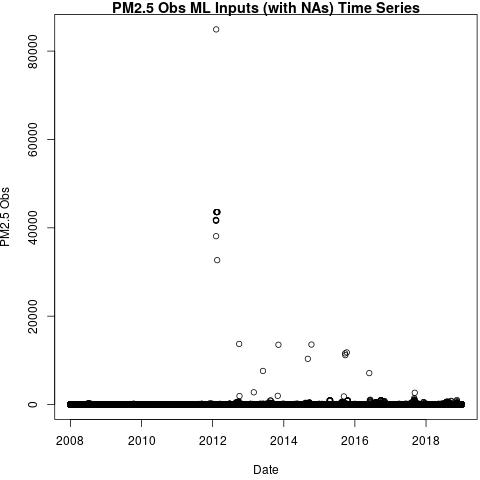
\includegraphics[width=0.77\textwidth]{Code_Outputs/Report_ML_input_PM25_Step4_part_f_de_duplicated_aveswNAs_PM25_ObsvDate.jpg} 
\caption{\label{fig:Report_ML_input_PM25_Step4_part_f_de_duplicated_aveswNAsPM25_ObsvDate}ML Inputs (with NAs) Time Series} 
\end{figure} 
 

\begin{figure} 
\centering  
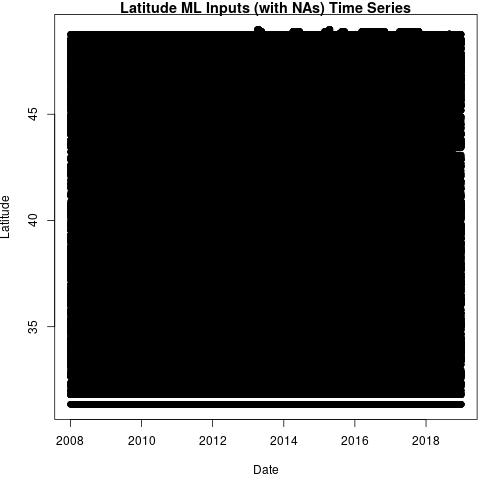
\includegraphics[width=0.77\textwidth]{Code_Outputs/Report_ML_input_PM25_Step4_part_f_de_duplicated_aveswNAs_LatitudevDate.jpg} 
\caption{\label{fig:Report_ML_input_PM25_Step4_part_f_de_duplicated_aveswNAsLatitudevDate}ML Inputs (with NAs) Time Series} 
\end{figure} 
 

\begin{figure} 
\centering  
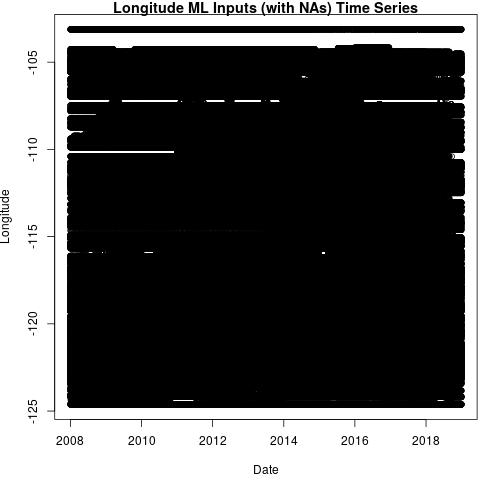
\includegraphics[width=0.77\textwidth]{Code_Outputs/Report_ML_input_PM25_Step4_part_f_de_duplicated_aveswNAs_LongitudevDate.jpg} 
\caption{\label{fig:Report_ML_input_PM25_Step4_part_f_de_duplicated_aveswNAsLongitudevDate}ML Inputs (with NAs) Time Series} 
\end{figure} 
 

\begin{figure} 
\centering  
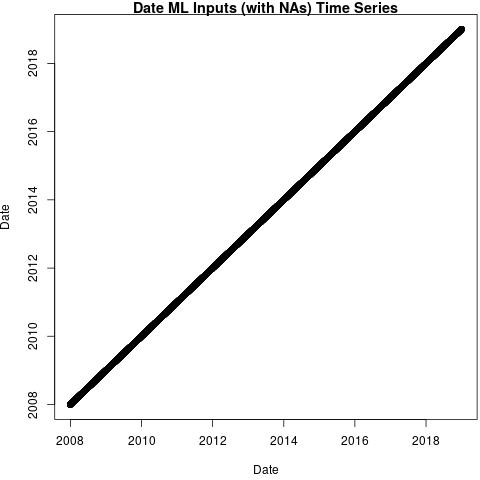
\includegraphics[width=0.77\textwidth]{Code_Outputs/Report_ML_input_PM25_Step4_part_f_de_duplicated_aveswNAs_DatevDate.jpg} 
\caption{\label{fig:Report_ML_input_PM25_Step4_part_f_de_duplicated_aveswNAsDatevDate}ML Inputs (with NAs) Time Series} 
\end{figure} 
 

\begin{figure} 
\centering  
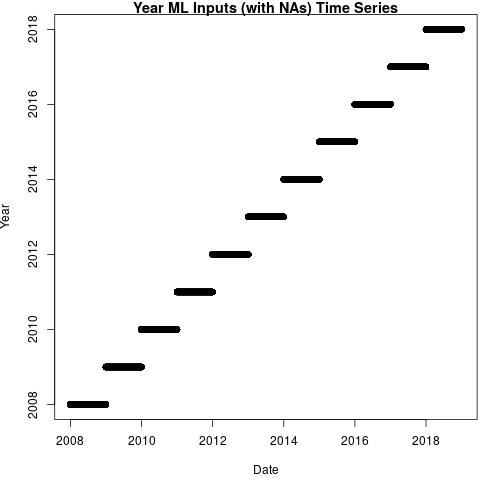
\includegraphics[width=0.77\textwidth]{Code_Outputs/Report_ML_input_PM25_Step4_part_f_de_duplicated_aveswNAs_YearvDate.jpg} 
\caption{\label{fig:Report_ML_input_PM25_Step4_part_f_de_duplicated_aveswNAsYearvDate}ML Inputs (with NAs) Time Series} 
\end{figure} 
 

\begin{figure} 
\centering  
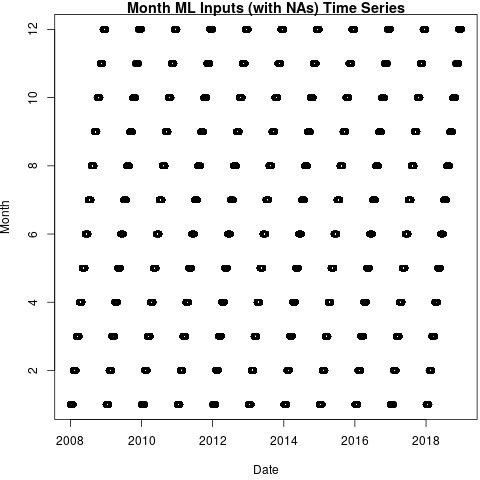
\includegraphics[width=0.77\textwidth]{Code_Outputs/Report_ML_input_PM25_Step4_part_f_de_duplicated_aveswNAs_MonthvDate.jpg} 
\caption{\label{fig:Report_ML_input_PM25_Step4_part_f_de_duplicated_aveswNAsMonthvDate}ML Inputs (with NAs) Time Series} 
\end{figure} 
 

\begin{figure} 
\centering  
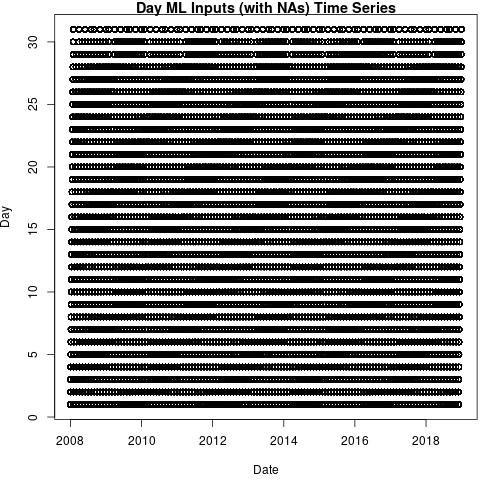
\includegraphics[width=0.77\textwidth]{Code_Outputs/Report_ML_input_PM25_Step4_part_f_de_duplicated_aveswNAs_DayvDate.jpg} 
\caption{\label{fig:Report_ML_input_PM25_Step4_part_f_de_duplicated_aveswNAsDayvDate}ML Inputs (with NAs) Time Series} 
\end{figure} 
 

\begin{figure} 
\centering  
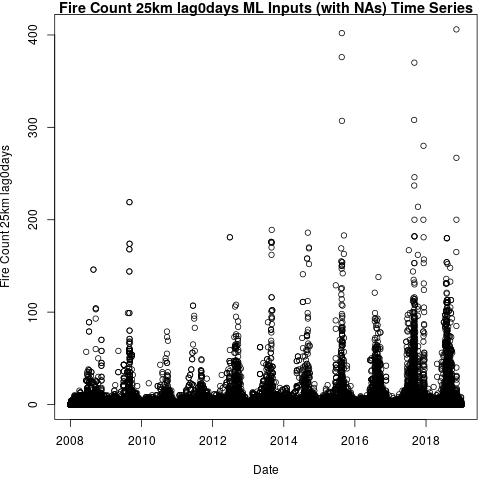
\includegraphics[width=0.77\textwidth]{Code_Outputs/Report_ML_input_PM25_Step4_part_f_de_duplicated_aveswNAs_Fire_Count_25km_lag0daysvDate.jpg} 
\caption{\label{fig:Report_ML_input_PM25_Step4_part_f_de_duplicated_aveswNAsFire_Count_25km_lag0daysvDate}ML Inputs (with NAs) Time Series} 
\end{figure} 
 

\begin{figure} 
\centering  
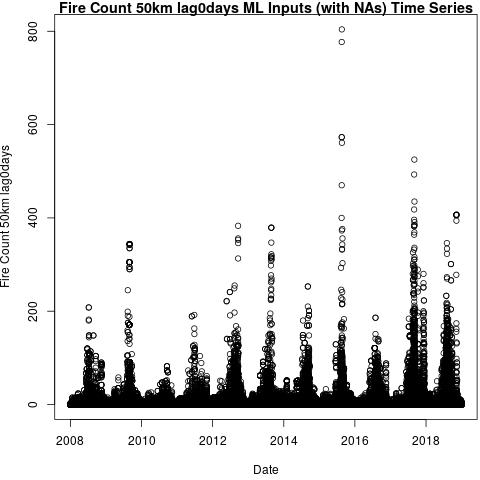
\includegraphics[width=0.77\textwidth]{Code_Outputs/Report_ML_input_PM25_Step4_part_f_de_duplicated_aveswNAs_Fire_Count_50km_lag0daysvDate.jpg} 
\caption{\label{fig:Report_ML_input_PM25_Step4_part_f_de_duplicated_aveswNAsFire_Count_50km_lag0daysvDate}ML Inputs (with NAs) Time Series} 
\end{figure} 
 

\clearpage 

\begin{figure} 
\centering  
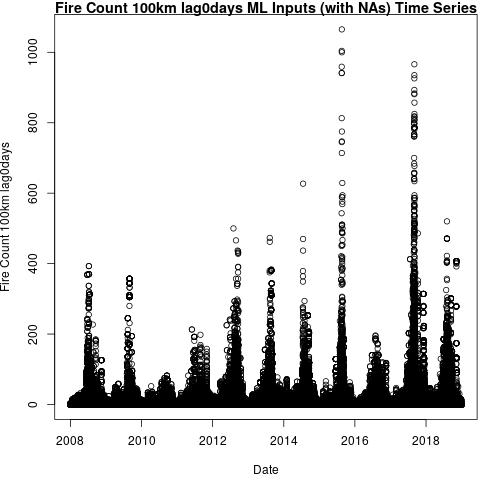
\includegraphics[width=0.77\textwidth]{Code_Outputs/Report_ML_input_PM25_Step4_part_f_de_duplicated_aveswNAs_Fire_Count_100km_lag0daysvDate.jpg} 
\caption{\label{fig:Report_ML_input_PM25_Step4_part_f_de_duplicated_aveswNAsFire_Count_100km_lag0daysvDate}ML Inputs (with NAs) Time Series} 
\end{figure} 
 

\begin{figure} 
\centering  
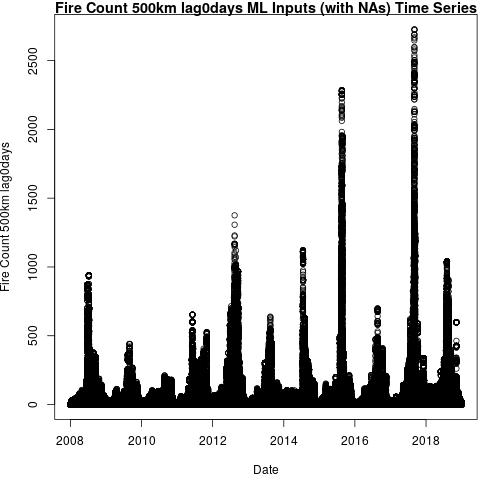
\includegraphics[width=0.77\textwidth]{Code_Outputs/Report_ML_input_PM25_Step4_part_f_de_duplicated_aveswNAs_Fire_Count_500km_lag0daysvDate.jpg} 
\caption{\label{fig:Report_ML_input_PM25_Step4_part_f_de_duplicated_aveswNAsFire_Count_500km_lag0daysvDate}ML Inputs (with NAs) Time Series} 
\end{figure} 
 

\begin{figure} 
\centering  
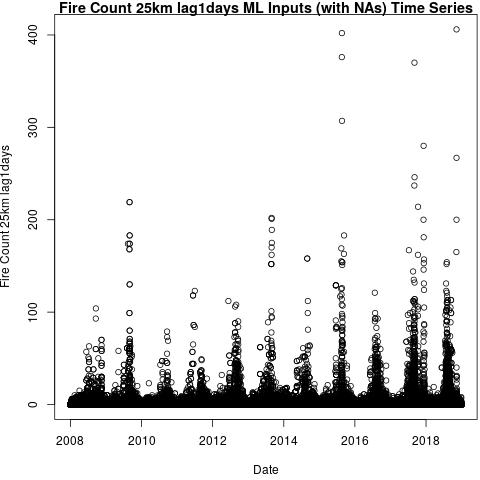
\includegraphics[width=0.77\textwidth]{Code_Outputs/Report_ML_input_PM25_Step4_part_f_de_duplicated_aveswNAs_Fire_Count_25km_lag1daysvDate.jpg} 
\caption{\label{fig:Report_ML_input_PM25_Step4_part_f_de_duplicated_aveswNAsFire_Count_25km_lag1daysvDate}ML Inputs (with NAs) Time Series} 
\end{figure} 
 

\begin{figure} 
\centering  
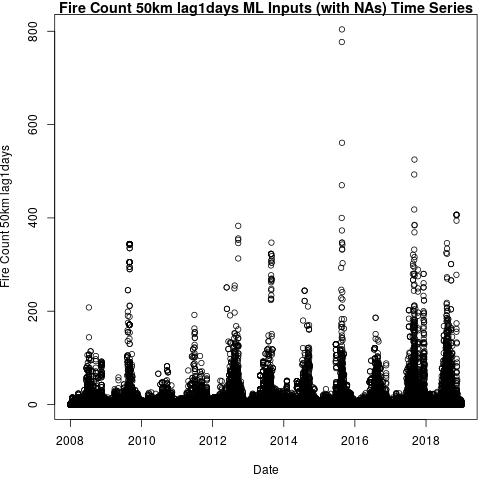
\includegraphics[width=0.77\textwidth]{Code_Outputs/Report_ML_input_PM25_Step4_part_f_de_duplicated_aveswNAs_Fire_Count_50km_lag1daysvDate.jpg} 
\caption{\label{fig:Report_ML_input_PM25_Step4_part_f_de_duplicated_aveswNAsFire_Count_50km_lag1daysvDate}ML Inputs (with NAs) Time Series} 
\end{figure} 
 

\begin{figure} 
\centering  
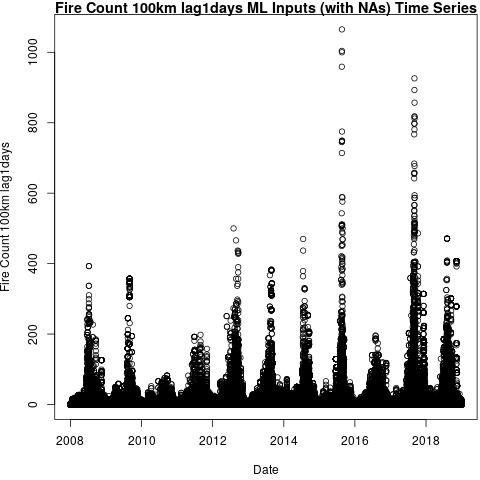
\includegraphics[width=0.77\textwidth]{Code_Outputs/Report_ML_input_PM25_Step4_part_f_de_duplicated_aveswNAs_Fire_Count_100km_lag1daysvDate.jpg} 
\caption{\label{fig:Report_ML_input_PM25_Step4_part_f_de_duplicated_aveswNAsFire_Count_100km_lag1daysvDate}ML Inputs (with NAs) Time Series} 
\end{figure} 
 

\begin{figure} 
\centering  
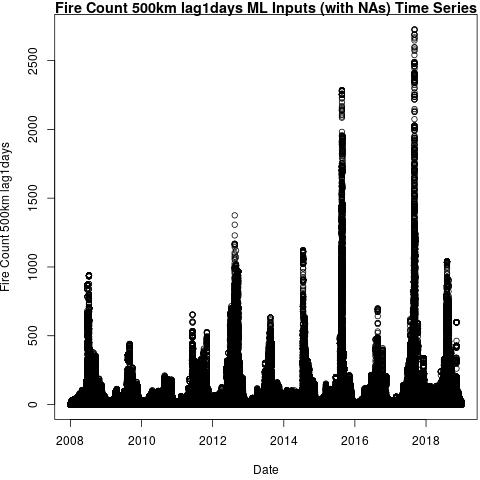
\includegraphics[width=0.77\textwidth]{Code_Outputs/Report_ML_input_PM25_Step4_part_f_de_duplicated_aveswNAs_Fire_Count_500km_lag1daysvDate.jpg} 
\caption{\label{fig:Report_ML_input_PM25_Step4_part_f_de_duplicated_aveswNAsFire_Count_500km_lag1daysvDate}ML Inputs (with NAs) Time Series} 
\end{figure} 
 

\begin{figure} 
\centering  
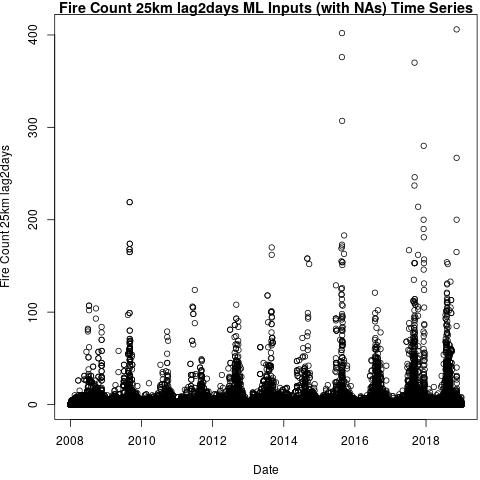
\includegraphics[width=0.77\textwidth]{Code_Outputs/Report_ML_input_PM25_Step4_part_f_de_duplicated_aveswNAs_Fire_Count_25km_lag2daysvDate.jpg} 
\caption{\label{fig:Report_ML_input_PM25_Step4_part_f_de_duplicated_aveswNAsFire_Count_25km_lag2daysvDate}ML Inputs (with NAs) Time Series} 
\end{figure} 
 

\begin{figure} 
\centering  
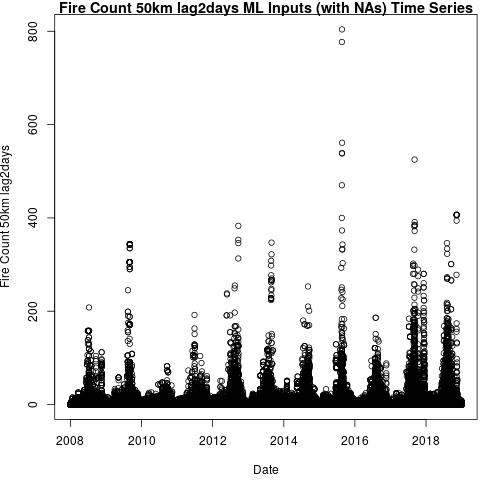
\includegraphics[width=0.77\textwidth]{Code_Outputs/Report_ML_input_PM25_Step4_part_f_de_duplicated_aveswNAs_Fire_Count_50km_lag2daysvDate.jpg} 
\caption{\label{fig:Report_ML_input_PM25_Step4_part_f_de_duplicated_aveswNAsFire_Count_50km_lag2daysvDate}ML Inputs (with NAs) Time Series} 
\end{figure} 
 

\begin{figure} 
\centering  
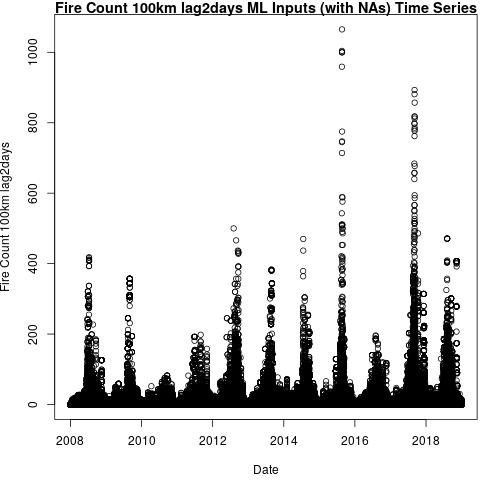
\includegraphics[width=0.77\textwidth]{Code_Outputs/Report_ML_input_PM25_Step4_part_f_de_duplicated_aveswNAs_Fire_Count_100km_lag2daysvDate.jpg} 
\caption{\label{fig:Report_ML_input_PM25_Step4_part_f_de_duplicated_aveswNAsFire_Count_100km_lag2daysvDate}ML Inputs (with NAs) Time Series} 
\end{figure} 
 

\begin{figure} 
\centering  
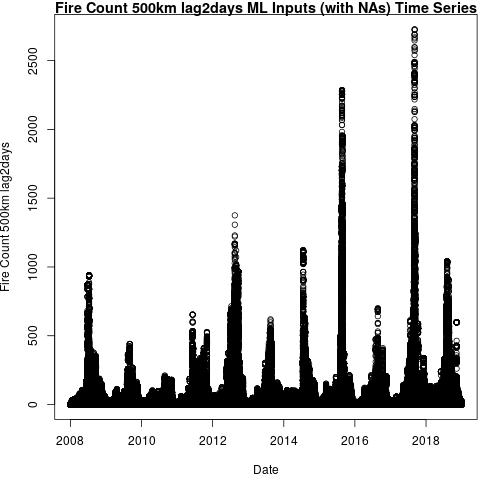
\includegraphics[width=0.77\textwidth]{Code_Outputs/Report_ML_input_PM25_Step4_part_f_de_duplicated_aveswNAs_Fire_Count_500km_lag2daysvDate.jpg} 
\caption{\label{fig:Report_ML_input_PM25_Step4_part_f_de_duplicated_aveswNAsFire_Count_500km_lag2daysvDate}ML Inputs (with NAs) Time Series} 
\end{figure} 
 

\clearpage 

\begin{figure} 
\centering  
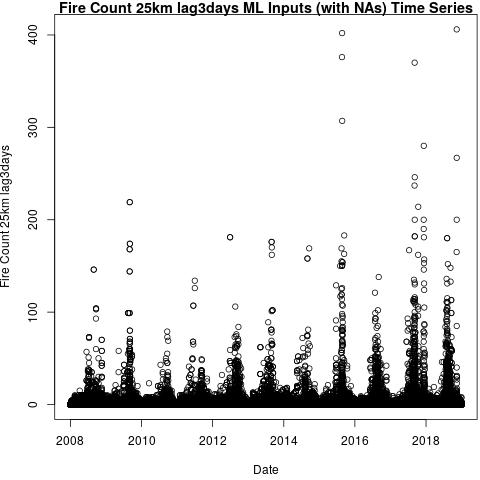
\includegraphics[width=0.77\textwidth]{Code_Outputs/Report_ML_input_PM25_Step4_part_f_de_duplicated_aveswNAs_Fire_Count_25km_lag3daysvDate.jpg} 
\caption{\label{fig:Report_ML_input_PM25_Step4_part_f_de_duplicated_aveswNAsFire_Count_25km_lag3daysvDate}ML Inputs (with NAs) Time Series} 
\end{figure} 
 

\begin{figure} 
\centering  
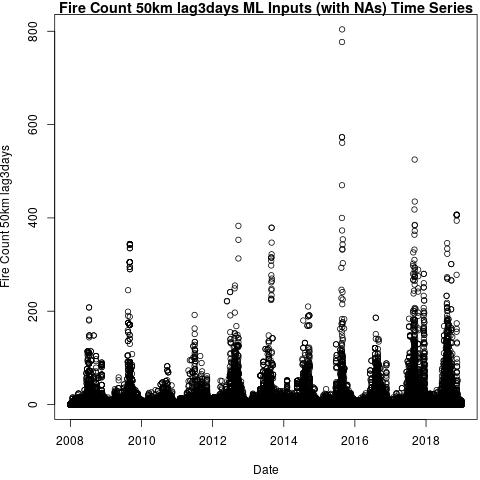
\includegraphics[width=0.77\textwidth]{Code_Outputs/Report_ML_input_PM25_Step4_part_f_de_duplicated_aveswNAs_Fire_Count_50km_lag3daysvDate.jpg} 
\caption{\label{fig:Report_ML_input_PM25_Step4_part_f_de_duplicated_aveswNAsFire_Count_50km_lag3daysvDate}ML Inputs (with NAs) Time Series} 
\end{figure} 
 

\begin{figure} 
\centering  
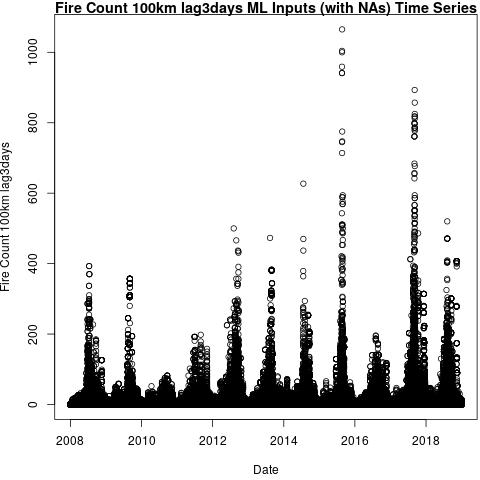
\includegraphics[width=0.77\textwidth]{Code_Outputs/Report_ML_input_PM25_Step4_part_f_de_duplicated_aveswNAs_Fire_Count_100km_lag3daysvDate.jpg} 
\caption{\label{fig:Report_ML_input_PM25_Step4_part_f_de_duplicated_aveswNAsFire_Count_100km_lag3daysvDate}ML Inputs (with NAs) Time Series} 
\end{figure} 
 

\begin{figure} 
\centering  
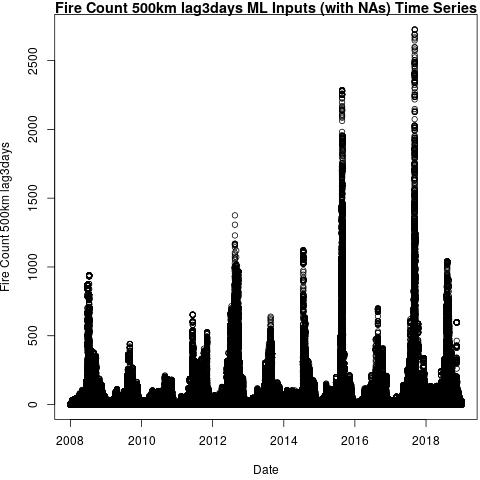
\includegraphics[width=0.77\textwidth]{Code_Outputs/Report_ML_input_PM25_Step4_part_f_de_duplicated_aveswNAs_Fire_Count_500km_lag3daysvDate.jpg} 
\caption{\label{fig:Report_ML_input_PM25_Step4_part_f_de_duplicated_aveswNAsFire_Count_500km_lag3daysvDate}ML Inputs (with NAs) Time Series} 
\end{figure} 
 

\begin{figure} 
\centering  
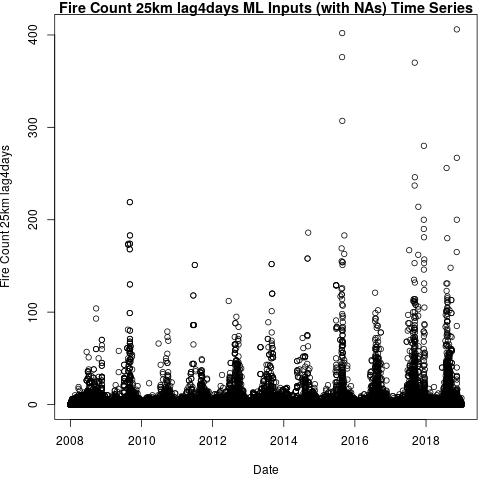
\includegraphics[width=0.77\textwidth]{Code_Outputs/Report_ML_input_PM25_Step4_part_f_de_duplicated_aveswNAs_Fire_Count_25km_lag4daysvDate.jpg} 
\caption{\label{fig:Report_ML_input_PM25_Step4_part_f_de_duplicated_aveswNAsFire_Count_25km_lag4daysvDate}ML Inputs (with NAs) Time Series} 
\end{figure} 
 

\begin{figure} 
\centering  
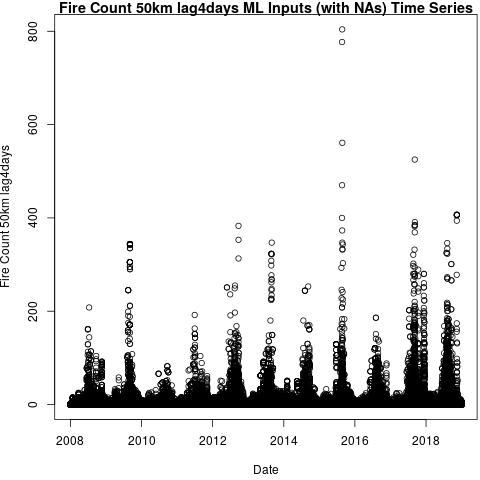
\includegraphics[width=0.77\textwidth]{Code_Outputs/Report_ML_input_PM25_Step4_part_f_de_duplicated_aveswNAs_Fire_Count_50km_lag4daysvDate.jpg} 
\caption{\label{fig:Report_ML_input_PM25_Step4_part_f_de_duplicated_aveswNAsFire_Count_50km_lag4daysvDate}ML Inputs (with NAs) Time Series} 
\end{figure} 
 

\begin{figure} 
\centering  
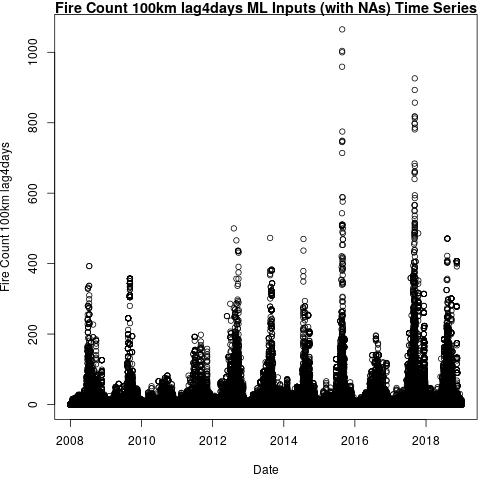
\includegraphics[width=0.77\textwidth]{Code_Outputs/Report_ML_input_PM25_Step4_part_f_de_duplicated_aveswNAs_Fire_Count_100km_lag4daysvDate.jpg} 
\caption{\label{fig:Report_ML_input_PM25_Step4_part_f_de_duplicated_aveswNAsFire_Count_100km_lag4daysvDate}ML Inputs (with NAs) Time Series} 
\end{figure} 
 

\begin{figure} 
\centering  
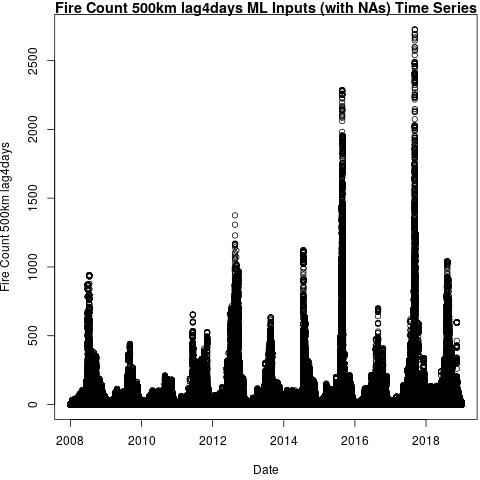
\includegraphics[width=0.77\textwidth]{Code_Outputs/Report_ML_input_PM25_Step4_part_f_de_duplicated_aveswNAs_Fire_Count_500km_lag4daysvDate.jpg} 
\caption{\label{fig:Report_ML_input_PM25_Step4_part_f_de_duplicated_aveswNAsFire_Count_500km_lag4daysvDate}ML Inputs (with NAs) Time Series} 
\end{figure} 
 

\begin{figure} 
\centering  
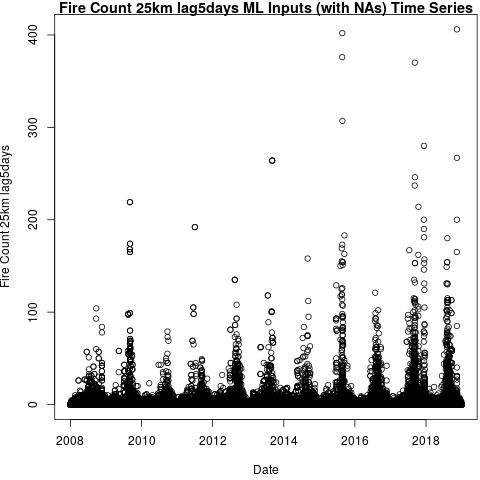
\includegraphics[width=0.77\textwidth]{Code_Outputs/Report_ML_input_PM25_Step4_part_f_de_duplicated_aveswNAs_Fire_Count_25km_lag5daysvDate.jpg} 
\caption{\label{fig:Report_ML_input_PM25_Step4_part_f_de_duplicated_aveswNAsFire_Count_25km_lag5daysvDate}ML Inputs (with NAs) Time Series} 
\end{figure} 
 

\begin{figure} 
\centering  
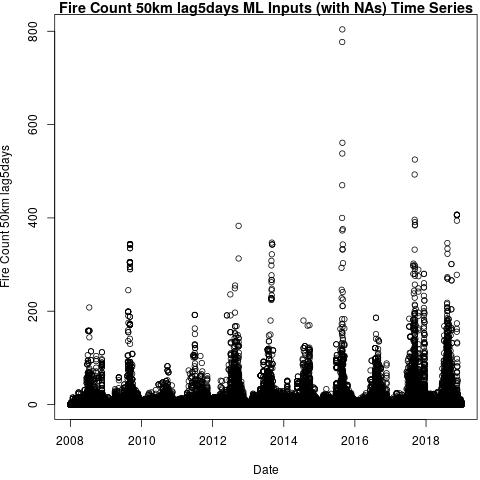
\includegraphics[width=0.77\textwidth]{Code_Outputs/Report_ML_input_PM25_Step4_part_f_de_duplicated_aveswNAs_Fire_Count_50km_lag5daysvDate.jpg} 
\caption{\label{fig:Report_ML_input_PM25_Step4_part_f_de_duplicated_aveswNAsFire_Count_50km_lag5daysvDate}ML Inputs (with NAs) Time Series} 
\end{figure} 
 

\clearpage 

\begin{figure} 
\centering  
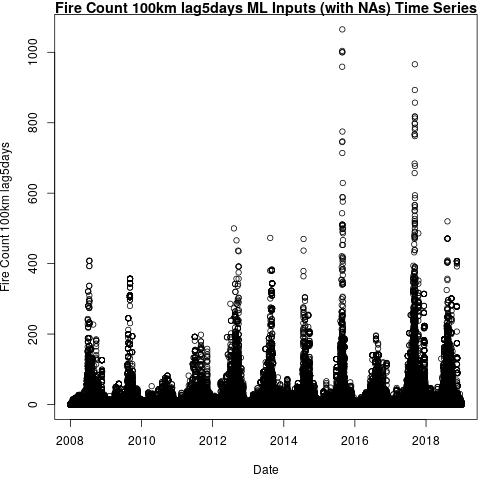
\includegraphics[width=0.77\textwidth]{Code_Outputs/Report_ML_input_PM25_Step4_part_f_de_duplicated_aveswNAs_Fire_Count_100km_lag5daysvDate.jpg} 
\caption{\label{fig:Report_ML_input_PM25_Step4_part_f_de_duplicated_aveswNAsFire_Count_100km_lag5daysvDate}ML Inputs (with NAs) Time Series} 
\end{figure} 
 

\begin{figure} 
\centering  
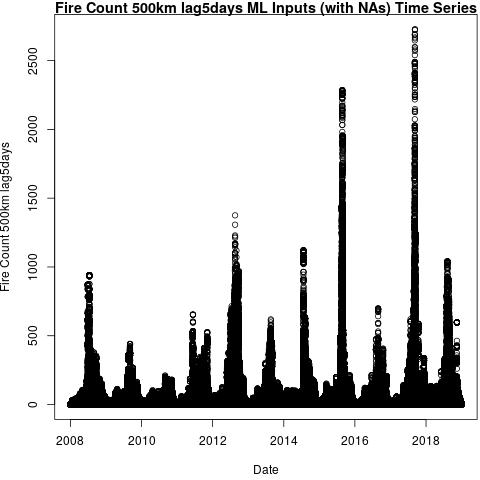
\includegraphics[width=0.77\textwidth]{Code_Outputs/Report_ML_input_PM25_Step4_part_f_de_duplicated_aveswNAs_Fire_Count_500km_lag5daysvDate.jpg} 
\caption{\label{fig:Report_ML_input_PM25_Step4_part_f_de_duplicated_aveswNAsFire_Count_500km_lag5daysvDate}ML Inputs (with NAs) Time Series} 
\end{figure} 
 

\begin{figure} 
\centering  
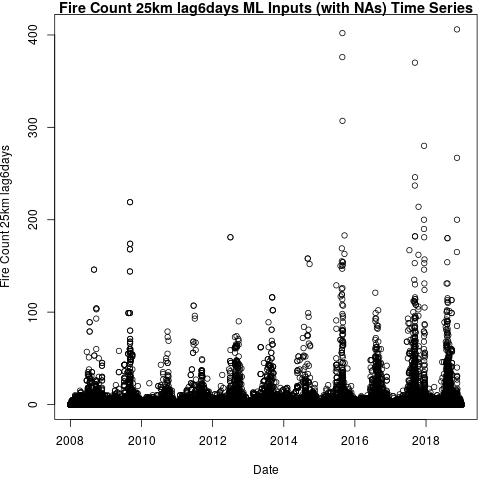
\includegraphics[width=0.77\textwidth]{Code_Outputs/Report_ML_input_PM25_Step4_part_f_de_duplicated_aveswNAs_Fire_Count_25km_lag6daysvDate.jpg} 
\caption{\label{fig:Report_ML_input_PM25_Step4_part_f_de_duplicated_aveswNAsFire_Count_25km_lag6daysvDate}ML Inputs (with NAs) Time Series} 
\end{figure} 
 

\begin{figure} 
\centering  
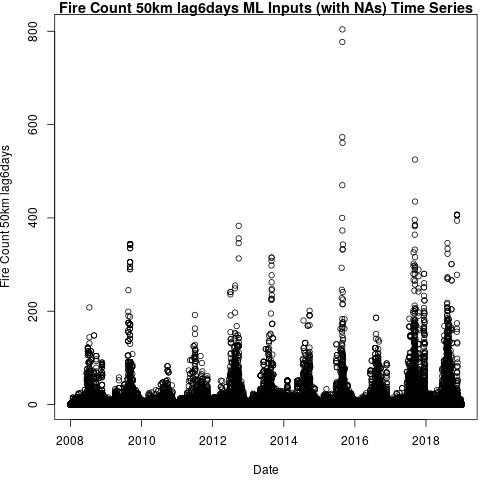
\includegraphics[width=0.77\textwidth]{Code_Outputs/Report_ML_input_PM25_Step4_part_f_de_duplicated_aveswNAs_Fire_Count_50km_lag6daysvDate.jpg} 
\caption{\label{fig:Report_ML_input_PM25_Step4_part_f_de_duplicated_aveswNAsFire_Count_50km_lag6daysvDate}ML Inputs (with NAs) Time Series} 
\end{figure} 
 

\begin{figure} 
\centering  
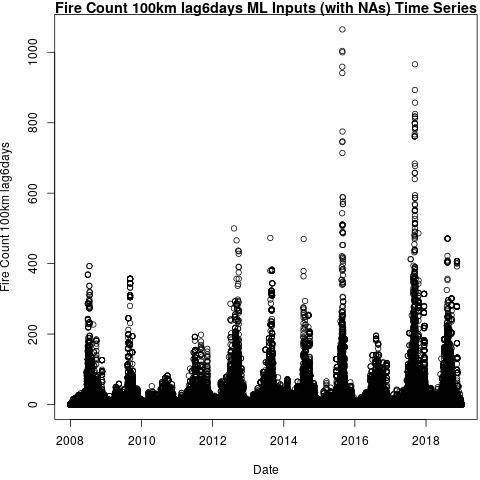
\includegraphics[width=0.77\textwidth]{Code_Outputs/Report_ML_input_PM25_Step4_part_f_de_duplicated_aveswNAs_Fire_Count_100km_lag6daysvDate.jpg} 
\caption{\label{fig:Report_ML_input_PM25_Step4_part_f_de_duplicated_aveswNAsFire_Count_100km_lag6daysvDate}ML Inputs (with NAs) Time Series} 
\end{figure} 
 

\begin{figure} 
\centering  
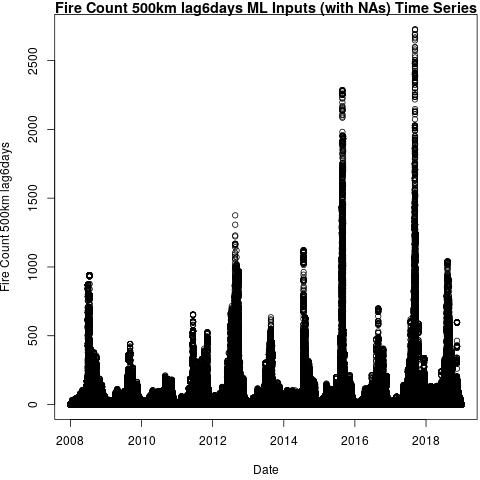
\includegraphics[width=0.77\textwidth]{Code_Outputs/Report_ML_input_PM25_Step4_part_f_de_duplicated_aveswNAs_Fire_Count_500km_lag6daysvDate.jpg} 
\caption{\label{fig:Report_ML_input_PM25_Step4_part_f_de_duplicated_aveswNAsFire_Count_500km_lag6daysvDate}ML Inputs (with NAs) Time Series} 
\end{figure} 
 

\begin{figure} 
\centering  
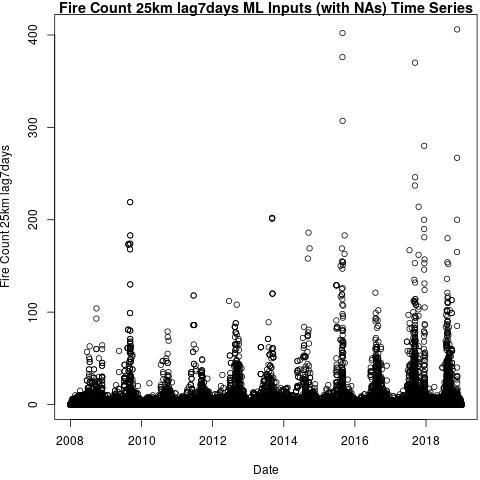
\includegraphics[width=0.77\textwidth]{Code_Outputs/Report_ML_input_PM25_Step4_part_f_de_duplicated_aveswNAs_Fire_Count_25km_lag7daysvDate.jpg} 
\caption{\label{fig:Report_ML_input_PM25_Step4_part_f_de_duplicated_aveswNAsFire_Count_25km_lag7daysvDate}ML Inputs (with NAs) Time Series} 
\end{figure} 
 

\begin{figure} 
\centering  
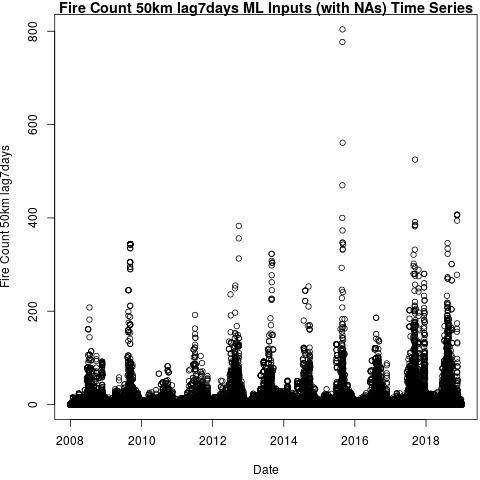
\includegraphics[width=0.77\textwidth]{Code_Outputs/Report_ML_input_PM25_Step4_part_f_de_duplicated_aveswNAs_Fire_Count_50km_lag7daysvDate.jpg} 
\caption{\label{fig:Report_ML_input_PM25_Step4_part_f_de_duplicated_aveswNAsFire_Count_50km_lag7daysvDate}ML Inputs (with NAs) Time Series} 
\end{figure} 
 

\begin{figure} 
\centering  
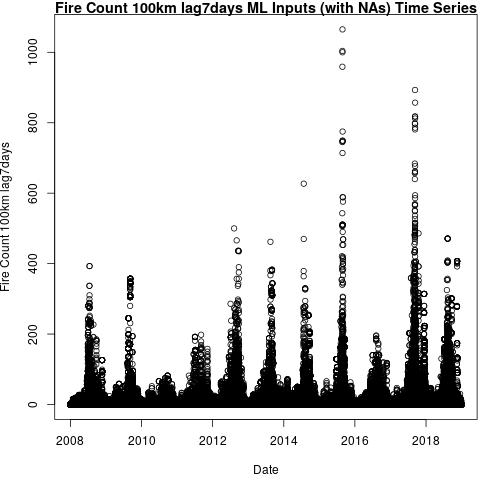
\includegraphics[width=0.77\textwidth]{Code_Outputs/Report_ML_input_PM25_Step4_part_f_de_duplicated_aveswNAs_Fire_Count_100km_lag7daysvDate.jpg} 
\caption{\label{fig:Report_ML_input_PM25_Step4_part_f_de_duplicated_aveswNAsFire_Count_100km_lag7daysvDate}ML Inputs (with NAs) Time Series} 
\end{figure} 
 

\begin{figure} 
\centering  
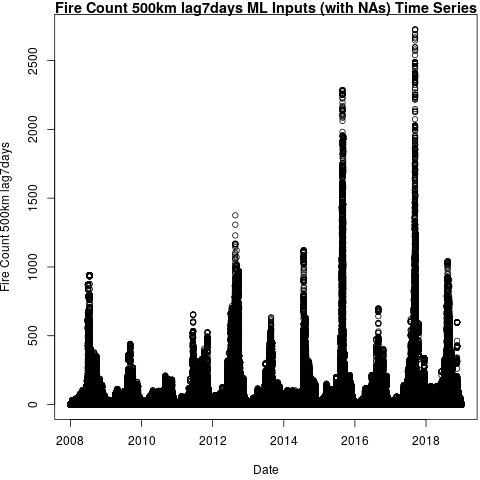
\includegraphics[width=0.77\textwidth]{Code_Outputs/Report_ML_input_PM25_Step4_part_f_de_duplicated_aveswNAs_Fire_Count_500km_lag7daysvDate.jpg} 
\caption{\label{fig:Report_ML_input_PM25_Step4_part_f_de_duplicated_aveswNAsFire_Count_500km_lag7daysvDate}ML Inputs (with NAs) Time Series} 
\end{figure} 
 

\clearpage 

\begin{figure} 
\centering  
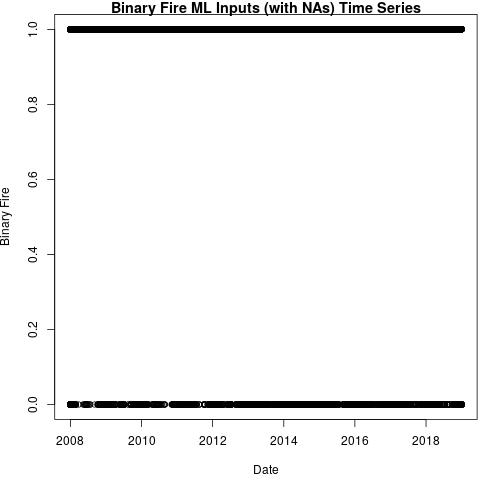
\includegraphics[width=0.77\textwidth]{Code_Outputs/Report_ML_input_PM25_Step4_part_f_de_duplicated_aveswNAs_Binary_FirevDate.jpg} 
\caption{\label{fig:Report_ML_input_PM25_Step4_part_f_de_duplicated_aveswNAsBinary_FirevDate}ML Inputs (with NAs) Time Series} 
\end{figure} 
 

\begin{figure} 
\centering  
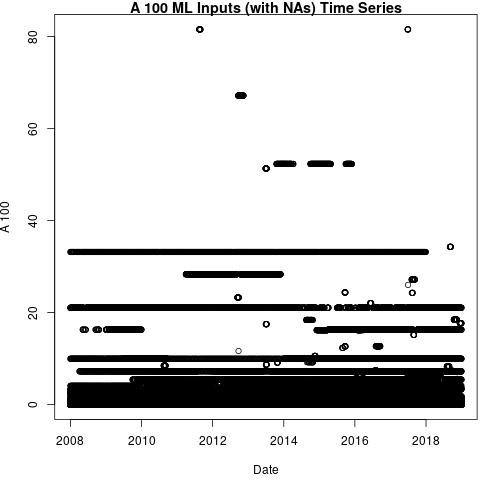
\includegraphics[width=0.77\textwidth]{Code_Outputs/Report_ML_input_PM25_Step4_part_f_de_duplicated_aveswNAs_A_100vDate.jpg} 
\caption{\label{fig:Report_ML_input_PM25_Step4_part_f_de_duplicated_aveswNAsA_100vDate}ML Inputs (with NAs) Time Series} 
\end{figure} 
 

\begin{figure} 
\centering  
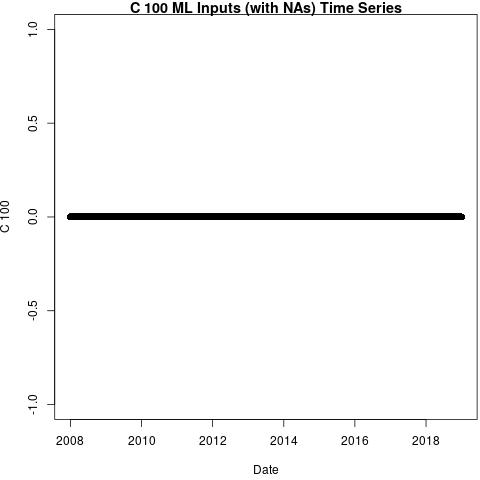
\includegraphics[width=0.77\textwidth]{Code_Outputs/Report_ML_input_PM25_Step4_part_f_de_duplicated_aveswNAs_C_100vDate.jpg} 
\caption{\label{fig:Report_ML_input_PM25_Step4_part_f_de_duplicated_aveswNAsC_100vDate}ML Inputs (with NAs) Time Series} 
\end{figure} 
 

\begin{figure} 
\centering  
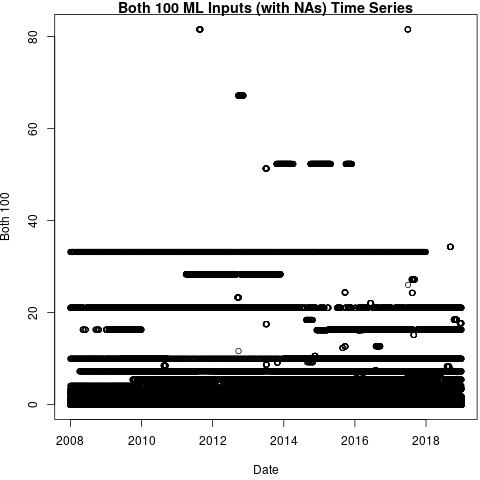
\includegraphics[width=0.77\textwidth]{Code_Outputs/Report_ML_input_PM25_Step4_part_f_de_duplicated_aveswNAs_Both_100vDate.jpg} 
\caption{\label{fig:Report_ML_input_PM25_Step4_part_f_de_duplicated_aveswNAsBoth_100vDate}ML Inputs (with NAs) Time Series} 
\end{figure} 
 

\begin{figure} 
\centering  
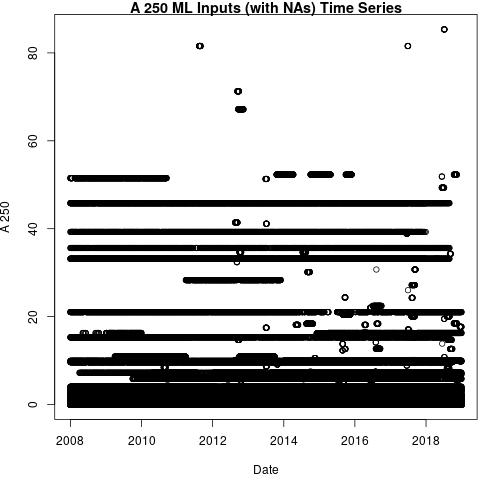
\includegraphics[width=0.77\textwidth]{Code_Outputs/Report_ML_input_PM25_Step4_part_f_de_duplicated_aveswNAs_A_250vDate.jpg} 
\caption{\label{fig:Report_ML_input_PM25_Step4_part_f_de_duplicated_aveswNAsA_250vDate}ML Inputs (with NAs) Time Series} 
\end{figure} 
 

\begin{figure} 
\centering  
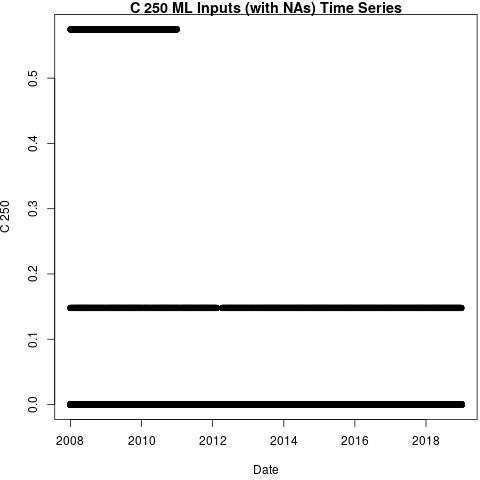
\includegraphics[width=0.77\textwidth]{Code_Outputs/Report_ML_input_PM25_Step4_part_f_de_duplicated_aveswNAs_C_250vDate.jpg} 
\caption{\label{fig:Report_ML_input_PM25_Step4_part_f_de_duplicated_aveswNAsC_250vDate}ML Inputs (with NAs) Time Series} 
\end{figure} 
 

\begin{figure} 
\centering  
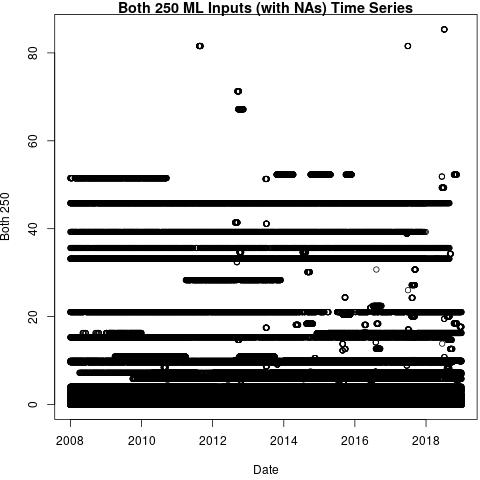
\includegraphics[width=0.77\textwidth]{Code_Outputs/Report_ML_input_PM25_Step4_part_f_de_duplicated_aveswNAs_Both_250vDate.jpg} 
\caption{\label{fig:Report_ML_input_PM25_Step4_part_f_de_duplicated_aveswNAsBoth_250vDate}ML Inputs (with NAs) Time Series} 
\end{figure} 
 

\begin{figure} 
\centering  
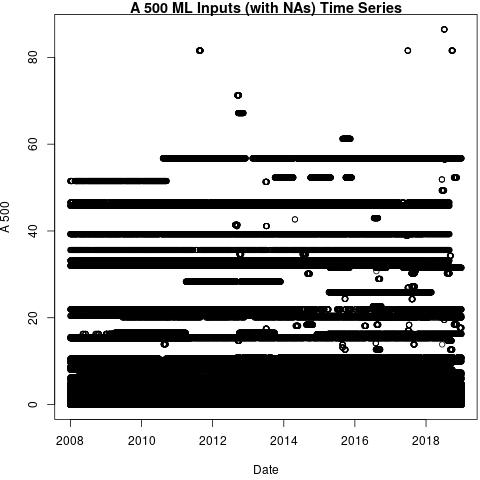
\includegraphics[width=0.77\textwidth]{Code_Outputs/Report_ML_input_PM25_Step4_part_f_de_duplicated_aveswNAs_A_500vDate.jpg} 
\caption{\label{fig:Report_ML_input_PM25_Step4_part_f_de_duplicated_aveswNAsA_500vDate}ML Inputs (with NAs) Time Series} 
\end{figure} 
 

\begin{figure} 
\centering  
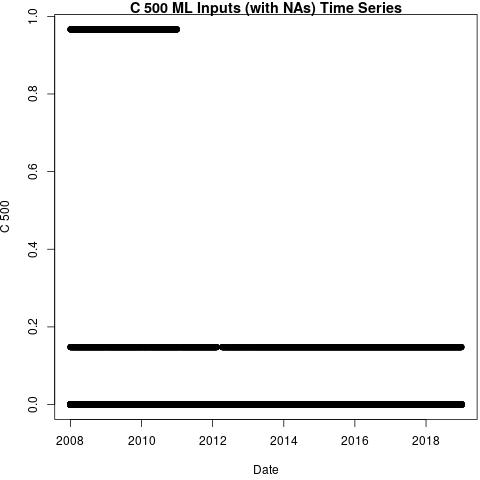
\includegraphics[width=0.77\textwidth]{Code_Outputs/Report_ML_input_PM25_Step4_part_f_de_duplicated_aveswNAs_C_500vDate.jpg} 
\caption{\label{fig:Report_ML_input_PM25_Step4_part_f_de_duplicated_aveswNAsC_500vDate}ML Inputs (with NAs) Time Series} 
\end{figure} 
 

\begin{figure} 
\centering  
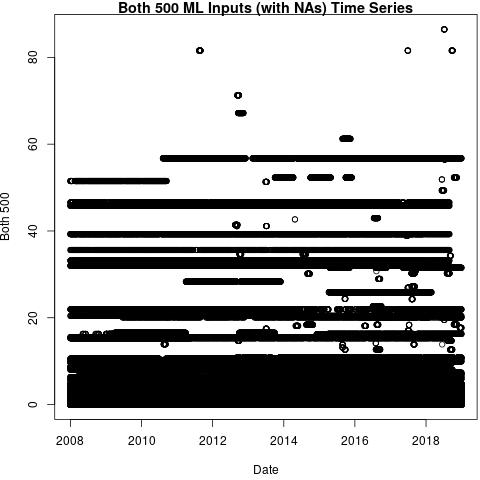
\includegraphics[width=0.77\textwidth]{Code_Outputs/Report_ML_input_PM25_Step4_part_f_de_duplicated_aveswNAs_Both_500vDate.jpg} 
\caption{\label{fig:Report_ML_input_PM25_Step4_part_f_de_duplicated_aveswNAsBoth_500vDate}ML Inputs (with NAs) Time Series} 
\end{figure} 
 

\clearpage 

\begin{figure} 
\centering  
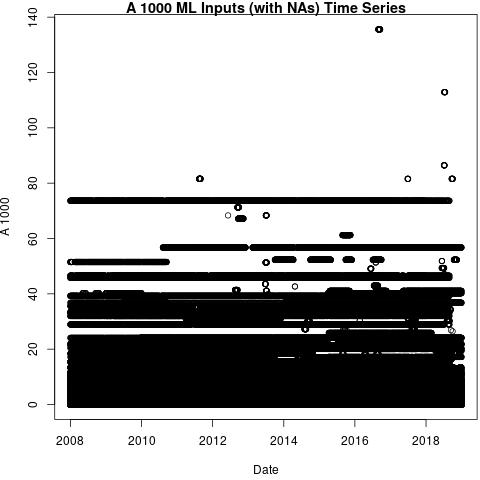
\includegraphics[width=0.77\textwidth]{Code_Outputs/Report_ML_input_PM25_Step4_part_f_de_duplicated_aveswNAs_A_1000vDate.jpg} 
\caption{\label{fig:Report_ML_input_PM25_Step4_part_f_de_duplicated_aveswNAsA_1000vDate}ML Inputs (with NAs) Time Series} 
\end{figure} 
 

\begin{figure} 
\centering  
\includegraphics[width=0.77\textwidth]{Code_Outputs/Report_ML_input_PM25_Step4_part_f_de_duplicated_aveswNAs_C_1000vDate.jpg} 
\caption{\label{fig:Report_ML_input_PM25_Step4_part_f_de_duplicated_aveswNAsC_1000vDate}ML Inputs (with NAs) Time Series} 
\end{figure} 
 

\begin{figure} 
\centering  
\includegraphics[width=0.77\textwidth]{Code_Outputs/Report_ML_input_PM25_Step4_part_f_de_duplicated_aveswNAs_Both_1000vDate.jpg} 
\caption{\label{fig:Report_ML_input_PM25_Step4_part_f_de_duplicated_aveswNAsBoth_1000vDate}ML Inputs (with NAs) Time Series} 
\end{figure} 
 

\begin{figure} 
\centering  
\includegraphics[width=0.77\textwidth]{Code_Outputs/Report_ML_input_PM25_Step4_part_f_de_duplicated_aveswNAs_Pop_densityvDate.jpg} 
\caption{\label{fig:Report_ML_input_PM25_Step4_part_f_de_duplicated_aveswNAsPop_densityvDate}ML Inputs (with NAs) Time Series} 
\end{figure} 
 

\begin{figure} 
\centering  
\includegraphics[width=0.77\textwidth]{Code_Outputs/Report_ML_input_PM25_Step4_part_f_de_duplicated_aveswNAs_MAIAC_AODvDate.jpg} 
\caption{\label{fig:Report_ML_input_PM25_Step4_part_f_de_duplicated_aveswNAsMAIAC_AODvDate}ML Inputs (with NAs) Time Series} 
\end{figure} 
 

\begin{figure} 
\centering  
\includegraphics[width=0.77\textwidth]{Code_Outputs/Report_ML_input_PM25_Step4_part_f_de_duplicated_aveswNAs_elevationvDate.jpg} 
\caption{\label{fig:Report_ML_input_PM25_Step4_part_f_de_duplicated_aveswNAselevationvDate}ML Inputs (with NAs) Time Series} 
\end{figure} 
 

\begin{figure} 
\centering  
\includegraphics[width=0.77\textwidth]{Code_Outputs/Report_ML_input_PM25_Step4_part_f_de_duplicated_aveswNAs_HPBLsurfacevDate.jpg} 
\caption{\label{fig:Report_ML_input_PM25_Step4_part_f_de_duplicated_aveswNAsHPBLsurfacevDate}ML Inputs (with NAs) Time Series} 
\end{figure} 
 

\begin{figure} 
\centering  
\includegraphics[width=0.77\textwidth]{Code_Outputs/Report_ML_input_PM25_Step4_part_f_de_duplicated_aveswNAs_TMP2mabovegroundvDate.jpg} 
\caption{\label{fig:Report_ML_input_PM25_Step4_part_f_de_duplicated_aveswNAsTMP2mabovegroundvDate}ML Inputs (with NAs) Time Series} 
\end{figure} 
 

\begin{figure} 
\centering  
\includegraphics[width=0.77\textwidth]{Code_Outputs/Report_ML_input_PM25_Step4_part_f_de_duplicated_aveswNAs_RH2mabovegroundvDate.jpg} 
\caption{\label{fig:Report_ML_input_PM25_Step4_part_f_de_duplicated_aveswNAsRH2mabovegroundvDate}ML Inputs (with NAs) Time Series} 
\end{figure} 
 

\begin{figure} 
\centering  
\includegraphics[width=0.77\textwidth]{Code_Outputs/Report_ML_input_PM25_Step4_part_f_de_duplicated_aveswNAs_DPT2mabovegroundvDate.jpg} 
\caption{\label{fig:Report_ML_input_PM25_Step4_part_f_de_duplicated_aveswNAsDPT2mabovegroundvDate}ML Inputs (with NAs) Time Series} 
\end{figure} 
 

\clearpage 

\begin{figure} 
\centering  
\includegraphics[width=0.77\textwidth]{Code_Outputs/Report_ML_input_PM25_Step4_part_f_de_duplicated_aveswNAs_APCPsurfacevDate.jpg} 
\caption{\label{fig:Report_ML_input_PM25_Step4_part_f_de_duplicated_aveswNAsAPCPsurfacevDate}ML Inputs (with NAs) Time Series} 
\end{figure} 
 

\begin{figure} 
\centering  
\includegraphics[width=0.77\textwidth]{Code_Outputs/Report_ML_input_PM25_Step4_part_f_de_duplicated_aveswNAs_WEASDsurfacevDate.jpg} 
\caption{\label{fig:Report_ML_input_PM25_Step4_part_f_de_duplicated_aveswNAsWEASDsurfacevDate}ML Inputs (with NAs) Time Series} 
\end{figure} 
 

\begin{figure} 
\centering  
\includegraphics[width=0.77\textwidth]{Code_Outputs/Report_ML_input_PM25_Step4_part_f_de_duplicated_aveswNAs_SNOWCsurfacevDate.jpg} 
\caption{\label{fig:Report_ML_input_PM25_Step4_part_f_de_duplicated_aveswNAsSNOWCsurfacevDate}ML Inputs (with NAs) Time Series} 
\end{figure} 
 

\begin{figure} 
\centering  
\includegraphics[width=0.77\textwidth]{Code_Outputs/Report_ML_input_PM25_Step4_part_f_de_duplicated_aveswNAs_UGRD10mabovegroundvDate.jpg} 
\caption{\label{fig:Report_ML_input_PM25_Step4_part_f_de_duplicated_aveswNAsUGRD10mabovegroundvDate}ML Inputs (with NAs) Time Series} 
\end{figure} 
 

\begin{figure} 
\centering  
\includegraphics[width=0.77\textwidth]{Code_Outputs/Report_ML_input_PM25_Step4_part_f_de_duplicated_aveswNAs_VGRD10mabovegroundvDate.jpg} 
\caption{\label{fig:Report_ML_input_PM25_Step4_part_f_de_duplicated_aveswNAsVGRD10mabovegroundvDate}ML Inputs (with NAs) Time Series} 
\end{figure} 
 

\begin{figure} 
\centering  
\includegraphics[width=0.77\textwidth]{Code_Outputs/Report_ML_input_PM25_Step4_part_f_de_duplicated_aveswNAs_PRMSLmeansealevelvDate.jpg} 
\caption{\label{fig:Report_ML_input_PM25_Step4_part_f_de_duplicated_aveswNAsPRMSLmeansealevelvDate}ML Inputs (with NAs) Time Series} 
\end{figure} 
 

\begin{figure} 
\centering  
\includegraphics[width=0.77\textwidth]{Code_Outputs/Report_ML_input_PM25_Step4_part_f_de_duplicated_aveswNAs_PRESsurfacevDate.jpg} 
\caption{\label{fig:Report_ML_input_PM25_Step4_part_f_de_duplicated_aveswNAsPRESsurfacevDate}ML Inputs (with NAs) Time Series} 
\end{figure} 
 

\begin{figure} 
\centering  
\includegraphics[width=0.77\textwidth]{Code_Outputs/Report_ML_input_PM25_Step4_part_f_de_duplicated_aveswNAs_DZDT850mbvDate.jpg} 
\caption{\label{fig:Report_ML_input_PM25_Step4_part_f_de_duplicated_aveswNAsDZDT850mbvDate}ML Inputs (with NAs) Time Series} 
\end{figure} 
 

\begin{figure} 
\centering  
\includegraphics[width=0.77\textwidth]{Code_Outputs/Report_ML_input_PM25_Step4_part_f_de_duplicated_aveswNAs_DZDT700mbvDate.jpg} 
\caption{\label{fig:Report_ML_input_PM25_Step4_part_f_de_duplicated_aveswNAsDZDT700mbvDate}ML Inputs (with NAs) Time Series} 
\end{figure} 
 

\begin{figure} 
\centering  
\includegraphics[width=0.77\textwidth]{Code_Outputs/Report_ML_input_PM25_Step4_part_f_de_duplicated_aveswNAs_NLCD_1km_percent_urban_buffervDate.jpg} 
\caption{\label{fig:Report_ML_input_PM25_Step4_part_f_de_duplicated_aveswNAsNLCD_1km_percent_urban_buffervDate}ML Inputs (with NAs) Time Series} 
\end{figure} 
 

\clearpage 

\begin{figure} 
\centering  
\includegraphics[width=0.77\textwidth]{Code_Outputs/Report_ML_input_PM25_Step4_part_f_de_duplicated_aveswNAs_NLCD_5km_percent_urban_buffervDate.jpg} 
\caption{\label{fig:Report_ML_input_PM25_Step4_part_f_de_duplicated_aveswNAsNLCD_5km_percent_urban_buffervDate}ML Inputs (with NAs) Time Series} 
\end{figure} 
 

\begin{figure} 
\centering  
\includegraphics[width=0.77\textwidth]{Code_Outputs/Report_ML_input_PM25_Step4_part_f_de_duplicated_aveswNAs_NLCD_10km_percent_urban_buffervDate.jpg} 
\caption{\label{fig:Report_ML_input_PM25_Step4_part_f_de_duplicated_aveswNAsNLCD_10km_percent_urban_buffervDate}ML Inputs (with NAs) Time Series} 
\end{figure} 
 

\begin{figure} 
\centering  
\includegraphics[width=0.77\textwidth]{Code_Outputs/Report_ML_input_PM25_Step4_part_f_de_duplicated_aveswNAs_NDVIvDate.jpg} 
\caption{\label{fig:Report_ML_input_PM25_Step4_part_f_de_duplicated_aveswNAsNDVIvDate}ML Inputs (with NAs) Time Series} 
\end{figure} 
 

\begin{figure} 
\centering  
\includegraphics[width=0.77\textwidth]{Code_Outputs/Report_ML_input_PM25_Step4_part_f_de_duplicated_aveswNAs_DayOfWeekvDate.jpg} 
\caption{\label{fig:Report_ML_input_PM25_Step4_part_f_de_duplicated_aveswNAsDayOfWeekvDate}ML Inputs (with NAs) Time Series} 
\end{figure} 
 

\begin{figure} 
\centering  
\includegraphics[width=0.77\textwidth]{Code_Outputs/Report_ML_input_PM25_Step4_part_f_de_duplicated_aveswNAs_WintervDate.jpg} 
\caption{\label{fig:Report_ML_input_PM25_Step4_part_f_de_duplicated_aveswNAsWintervDate}ML Inputs (with NAs) Time Series} 
\end{figure} 
 

\begin{figure} 
\centering  
\includegraphics[width=0.77\textwidth]{Code_Outputs/Report_ML_input_PM25_Step4_part_f_de_duplicated_aveswNAs_SpringvDate.jpg} 
\caption{\label{fig:Report_ML_input_PM25_Step4_part_f_de_duplicated_aveswNAsSpringvDate}ML Inputs (with NAs) Time Series} 
\end{figure} 
 

\begin{figure} 
\centering  
\includegraphics[width=0.77\textwidth]{Code_Outputs/Report_ML_input_PM25_Step4_part_f_de_duplicated_aveswNAs_SummervDate.jpg} 
\caption{\label{fig:Report_ML_input_PM25_Step4_part_f_de_duplicated_aveswNAsSummervDate}ML Inputs (with NAs) Time Series} 
\end{figure} 
 

\begin{figure} 
\centering  
\includegraphics[width=0.77\textwidth]{Code_Outputs/Report_ML_input_PM25_Step4_part_f_de_duplicated_aveswNAs_FallvDate.jpg} 
\caption{\label{fig:Report_ML_input_PM25_Step4_part_f_de_duplicated_aveswNAsFallvDate}ML Inputs (with NAs) Time Series} 
\end{figure} 
 

\begin{figure} 
\centering  
\includegraphics[width=0.77\textwidth]{Code_Outputs/Report_ML_input_PM25_Step4_part_f_de_duplicated_aveswNAs_StatevDate.jpg} 
\caption{\label{fig:Report_ML_input_PM25_Step4_part_f_de_duplicated_aveswNAsStatevDate}ML Inputs (with NAs) Time Series} 
\end{figure} 
 

\begin{figure} 
\centering  
\includegraphics[width=0.77\textwidth]{Code_Outputs/Report_ML_input_PM25_Step4_part_f_de_duplicated_aveswNAs_CosDOYvDate.jpg} 
\caption{\label{fig:Report_ML_input_PM25_Step4_part_f_de_duplicated_aveswNAsCosDOYvDate}ML Inputs (with NAs) Time Series} 
\end{figure} 
 
 

% PM2.5 vs predictor for each predictor variable 

\subsection{ML Inputs (with NAs) Plot against PM2.5 Obs Images} 
 

\begin{figure} 
\centering  
\includegraphics[width=0.77\textwidth]{Code_Outputs/Report_ML_input_PM25_Step4_part_f_de_duplicated_aveswNAs_Fire_Count_25km_lag0daysvPM25_Obs.jpg} 
\caption{\label{fig:Report_ML_input_PM25_Step4_part_f_de_duplicated_aveswNAsFire_Count_25km_lag0daysvPM25_Obs}ML Inputs (with NAs) Plot against PM2.5 Obs} 
\end{figure} 
 

\begin{figure} 
\centering  
\includegraphics[width=0.77\textwidth]{Code_Outputs/Report_ML_input_PM25_Step4_part_f_de_duplicated_aveswNAs_Fire_Count_50km_lag0daysvPM25_Obs.jpg} 
\caption{\label{fig:Report_ML_input_PM25_Step4_part_f_de_duplicated_aveswNAsFire_Count_50km_lag0daysvPM25_Obs}ML Inputs (with NAs) Plot against PM2.5 Obs} 
\end{figure} 
 

\begin{figure} 
\centering  
\includegraphics[width=0.77\textwidth]{Code_Outputs/Report_ML_input_PM25_Step4_part_f_de_duplicated_aveswNAs_Fire_Count_100km_lag0daysvPM25_Obs.jpg} 
\caption{\label{fig:Report_ML_input_PM25_Step4_part_f_de_duplicated_aveswNAsFire_Count_100km_lag0daysvPM25_Obs}ML Inputs (with NAs) Plot against PM2.5 Obs} 
\end{figure} 
 

\begin{figure} 
\centering  
\includegraphics[width=0.77\textwidth]{Code_Outputs/Report_ML_input_PM25_Step4_part_f_de_duplicated_aveswNAs_Fire_Count_500km_lag0daysvPM25_Obs.jpg} 
\caption{\label{fig:Report_ML_input_PM25_Step4_part_f_de_duplicated_aveswNAsFire_Count_500km_lag0daysvPM25_Obs}ML Inputs (with NAs) Plot against PM2.5 Obs} 
\end{figure} 
 

\begin{figure} 
\centering  
\includegraphics[width=0.77\textwidth]{Code_Outputs/Report_ML_input_PM25_Step4_part_f_de_duplicated_aveswNAs_Fire_Count_25km_lag1daysvPM25_Obs.jpg} 
\caption{\label{fig:Report_ML_input_PM25_Step4_part_f_de_duplicated_aveswNAsFire_Count_25km_lag1daysvPM25_Obs}ML Inputs (with NAs) Plot against PM2.5 Obs} 
\end{figure} 
 

\begin{figure} 
\centering  
\includegraphics[width=0.77\textwidth]{Code_Outputs/Report_ML_input_PM25_Step4_part_f_de_duplicated_aveswNAs_Fire_Count_50km_lag1daysvPM25_Obs.jpg} 
\caption{\label{fig:Report_ML_input_PM25_Step4_part_f_de_duplicated_aveswNAsFire_Count_50km_lag1daysvPM25_Obs}ML Inputs (with NAs) Plot against PM2.5 Obs} 
\end{figure} 
 

\begin{figure} 
\centering  
\includegraphics[width=0.77\textwidth]{Code_Outputs/Report_ML_input_PM25_Step4_part_f_de_duplicated_aveswNAs_Fire_Count_100km_lag1daysvPM25_Obs.jpg} 
\caption{\label{fig:Report_ML_input_PM25_Step4_part_f_de_duplicated_aveswNAsFire_Count_100km_lag1daysvPM25_Obs}ML Inputs (with NAs) Plot against PM2.5 Obs} 
\end{figure} 
 

\begin{figure} 
\centering  
\includegraphics[width=0.77\textwidth]{Code_Outputs/Report_ML_input_PM25_Step4_part_f_de_duplicated_aveswNAs_Fire_Count_500km_lag1daysvPM25_Obs.jpg} 
\caption{\label{fig:Report_ML_input_PM25_Step4_part_f_de_duplicated_aveswNAsFire_Count_500km_lag1daysvPM25_Obs}ML Inputs (with NAs) Plot against PM2.5 Obs} 
\end{figure} 
 

\begin{figure} 
\centering  
\includegraphics[width=0.77\textwidth]{Code_Outputs/Report_ML_input_PM25_Step4_part_f_de_duplicated_aveswNAs_Fire_Count_25km_lag2daysvPM25_Obs.jpg} 
\caption{\label{fig:Report_ML_input_PM25_Step4_part_f_de_duplicated_aveswNAsFire_Count_25km_lag2daysvPM25_Obs}ML Inputs (with NAs) Plot against PM2.5 Obs} 
\end{figure} 
 

\clearpage 

\begin{figure} 
\centering  
\includegraphics[width=0.77\textwidth]{Code_Outputs/Report_ML_input_PM25_Step4_part_f_de_duplicated_aveswNAs_Fire_Count_50km_lag2daysvPM25_Obs.jpg} 
\caption{\label{fig:Report_ML_input_PM25_Step4_part_f_de_duplicated_aveswNAsFire_Count_50km_lag2daysvPM25_Obs}ML Inputs (with NAs) Plot against PM2.5 Obs} 
\end{figure} 
 

\begin{figure} 
\centering  
\includegraphics[width=0.77\textwidth]{Code_Outputs/Report_ML_input_PM25_Step4_part_f_de_duplicated_aveswNAs_Fire_Count_100km_lag2daysvPM25_Obs.jpg} 
\caption{\label{fig:Report_ML_input_PM25_Step4_part_f_de_duplicated_aveswNAsFire_Count_100km_lag2daysvPM25_Obs}ML Inputs (with NAs) Plot against PM2.5 Obs} 
\end{figure} 
 

\begin{figure} 
\centering  
\includegraphics[width=0.77\textwidth]{Code_Outputs/Report_ML_input_PM25_Step4_part_f_de_duplicated_aveswNAs_Fire_Count_500km_lag2daysvPM25_Obs.jpg} 
\caption{\label{fig:Report_ML_input_PM25_Step4_part_f_de_duplicated_aveswNAsFire_Count_500km_lag2daysvPM25_Obs}ML Inputs (with NAs) Plot against PM2.5 Obs} 
\end{figure} 
 

\begin{figure} 
\centering  
\includegraphics[width=0.77\textwidth]{Code_Outputs/Report_ML_input_PM25_Step4_part_f_de_duplicated_aveswNAs_Fire_Count_25km_lag3daysvPM25_Obs.jpg} 
\caption{\label{fig:Report_ML_input_PM25_Step4_part_f_de_duplicated_aveswNAsFire_Count_25km_lag3daysvPM25_Obs}ML Inputs (with NAs) Plot against PM2.5 Obs} 
\end{figure} 
 

\begin{figure} 
\centering  
\includegraphics[width=0.77\textwidth]{Code_Outputs/Report_ML_input_PM25_Step4_part_f_de_duplicated_aveswNAs_Fire_Count_50km_lag3daysvPM25_Obs.jpg} 
\caption{\label{fig:Report_ML_input_PM25_Step4_part_f_de_duplicated_aveswNAsFire_Count_50km_lag3daysvPM25_Obs}ML Inputs (with NAs) Plot against PM2.5 Obs} 
\end{figure} 
 

\begin{figure} 
\centering  
\includegraphics[width=0.77\textwidth]{Code_Outputs/Report_ML_input_PM25_Step4_part_f_de_duplicated_aveswNAs_Fire_Count_100km_lag3daysvPM25_Obs.jpg} 
\caption{\label{fig:Report_ML_input_PM25_Step4_part_f_de_duplicated_aveswNAsFire_Count_100km_lag3daysvPM25_Obs}ML Inputs (with NAs) Plot against PM2.5 Obs} 
\end{figure} 
 

\begin{figure} 
\centering  
\includegraphics[width=0.77\textwidth]{Code_Outputs/Report_ML_input_PM25_Step4_part_f_de_duplicated_aveswNAs_Fire_Count_500km_lag3daysvPM25_Obs.jpg} 
\caption{\label{fig:Report_ML_input_PM25_Step4_part_f_de_duplicated_aveswNAsFire_Count_500km_lag3daysvPM25_Obs}ML Inputs (with NAs) Plot against PM2.5 Obs} 
\end{figure} 
 

\begin{figure} 
\centering  
\includegraphics[width=0.77\textwidth]{Code_Outputs/Report_ML_input_PM25_Step4_part_f_de_duplicated_aveswNAs_Fire_Count_25km_lag4daysvPM25_Obs.jpg} 
\caption{\label{fig:Report_ML_input_PM25_Step4_part_f_de_duplicated_aveswNAsFire_Count_25km_lag4daysvPM25_Obs}ML Inputs (with NAs) Plot against PM2.5 Obs} 
\end{figure} 
 

\begin{figure} 
\centering  
\includegraphics[width=0.77\textwidth]{Code_Outputs/Report_ML_input_PM25_Step4_part_f_de_duplicated_aveswNAs_Fire_Count_50km_lag4daysvPM25_Obs.jpg} 
\caption{\label{fig:Report_ML_input_PM25_Step4_part_f_de_duplicated_aveswNAsFire_Count_50km_lag4daysvPM25_Obs}ML Inputs (with NAs) Plot against PM2.5 Obs} 
\end{figure} 
 

\begin{figure} 
\centering  
\includegraphics[width=0.77\textwidth]{Code_Outputs/Report_ML_input_PM25_Step4_part_f_de_duplicated_aveswNAs_Fire_Count_100km_lag4daysvPM25_Obs.jpg} 
\caption{\label{fig:Report_ML_input_PM25_Step4_part_f_de_duplicated_aveswNAsFire_Count_100km_lag4daysvPM25_Obs}ML Inputs (with NAs) Plot against PM2.5 Obs} 
\end{figure} 
 

\clearpage 

\begin{figure} 
\centering  
\includegraphics[width=0.77\textwidth]{Code_Outputs/Report_ML_input_PM25_Step4_part_f_de_duplicated_aveswNAs_Fire_Count_500km_lag4daysvPM25_Obs.jpg} 
\caption{\label{fig:Report_ML_input_PM25_Step4_part_f_de_duplicated_aveswNAsFire_Count_500km_lag4daysvPM25_Obs}ML Inputs (with NAs) Plot against PM2.5 Obs} 
\end{figure} 
 

\begin{figure} 
\centering  
\includegraphics[width=0.77\textwidth]{Code_Outputs/Report_ML_input_PM25_Step4_part_f_de_duplicated_aveswNAs_Fire_Count_25km_lag5daysvPM25_Obs.jpg} 
\caption{\label{fig:Report_ML_input_PM25_Step4_part_f_de_duplicated_aveswNAsFire_Count_25km_lag5daysvPM25_Obs}ML Inputs (with NAs) Plot against PM2.5 Obs} 
\end{figure} 
 

\begin{figure} 
\centering  
\includegraphics[width=0.77\textwidth]{Code_Outputs/Report_ML_input_PM25_Step4_part_f_de_duplicated_aveswNAs_Fire_Count_50km_lag5daysvPM25_Obs.jpg} 
\caption{\label{fig:Report_ML_input_PM25_Step4_part_f_de_duplicated_aveswNAsFire_Count_50km_lag5daysvPM25_Obs}ML Inputs (with NAs) Plot against PM2.5 Obs} 
\end{figure} 
 

\begin{figure} 
\centering  
\includegraphics[width=0.77\textwidth]{Code_Outputs/Report_ML_input_PM25_Step4_part_f_de_duplicated_aveswNAs_Fire_Count_100km_lag5daysvPM25_Obs.jpg} 
\caption{\label{fig:Report_ML_input_PM25_Step4_part_f_de_duplicated_aveswNAsFire_Count_100km_lag5daysvPM25_Obs}ML Inputs (with NAs) Plot against PM2.5 Obs} 
\end{figure} 
 

\begin{figure} 
\centering  
\includegraphics[width=0.77\textwidth]{Code_Outputs/Report_ML_input_PM25_Step4_part_f_de_duplicated_aveswNAs_Fire_Count_500km_lag5daysvPM25_Obs.jpg} 
\caption{\label{fig:Report_ML_input_PM25_Step4_part_f_de_duplicated_aveswNAsFire_Count_500km_lag5daysvPM25_Obs}ML Inputs (with NAs) Plot against PM2.5 Obs} 
\end{figure} 
 

\begin{figure} 
\centering  
\includegraphics[width=0.77\textwidth]{Code_Outputs/Report_ML_input_PM25_Step4_part_f_de_duplicated_aveswNAs_Fire_Count_25km_lag6daysvPM25_Obs.jpg} 
\caption{\label{fig:Report_ML_input_PM25_Step4_part_f_de_duplicated_aveswNAsFire_Count_25km_lag6daysvPM25_Obs}ML Inputs (with NAs) Plot against PM2.5 Obs} 
\end{figure} 
 

\begin{figure} 
\centering  
\includegraphics[width=0.77\textwidth]{Code_Outputs/Report_ML_input_PM25_Step4_part_f_de_duplicated_aveswNAs_Fire_Count_50km_lag6daysvPM25_Obs.jpg} 
\caption{\label{fig:Report_ML_input_PM25_Step4_part_f_de_duplicated_aveswNAsFire_Count_50km_lag6daysvPM25_Obs}ML Inputs (with NAs) Plot against PM2.5 Obs} 
\end{figure} 
 

\begin{figure} 
\centering  
\includegraphics[width=0.77\textwidth]{Code_Outputs/Report_ML_input_PM25_Step4_part_f_de_duplicated_aveswNAs_Fire_Count_100km_lag6daysvPM25_Obs.jpg} 
\caption{\label{fig:Report_ML_input_PM25_Step4_part_f_de_duplicated_aveswNAsFire_Count_100km_lag6daysvPM25_Obs}ML Inputs (with NAs) Plot against PM2.5 Obs} 
\end{figure} 
 

\begin{figure} 
\centering  
\includegraphics[width=0.77\textwidth]{Code_Outputs/Report_ML_input_PM25_Step4_part_f_de_duplicated_aveswNAs_Fire_Count_500km_lag6daysvPM25_Obs.jpg} 
\caption{\label{fig:Report_ML_input_PM25_Step4_part_f_de_duplicated_aveswNAsFire_Count_500km_lag6daysvPM25_Obs}ML Inputs (with NAs) Plot against PM2.5 Obs} 
\end{figure} 
 

\begin{figure} 
\centering  
\includegraphics[width=0.77\textwidth]{Code_Outputs/Report_ML_input_PM25_Step4_part_f_de_duplicated_aveswNAs_Fire_Count_25km_lag7daysvPM25_Obs.jpg} 
\caption{\label{fig:Report_ML_input_PM25_Step4_part_f_de_duplicated_aveswNAsFire_Count_25km_lag7daysvPM25_Obs}ML Inputs (with NAs) Plot against PM2.5 Obs} 
\end{figure} 
 

\clearpage 

\begin{figure} 
\centering  
\includegraphics[width=0.77\textwidth]{Code_Outputs/Report_ML_input_PM25_Step4_part_f_de_duplicated_aveswNAs_Fire_Count_50km_lag7daysvPM25_Obs.jpg} 
\caption{\label{fig:Report_ML_input_PM25_Step4_part_f_de_duplicated_aveswNAsFire_Count_50km_lag7daysvPM25_Obs}ML Inputs (with NAs) Plot against PM2.5 Obs} 
\end{figure} 
 

\begin{figure} 
\centering  
\includegraphics[width=0.77\textwidth]{Code_Outputs/Report_ML_input_PM25_Step4_part_f_de_duplicated_aveswNAs_Fire_Count_100km_lag7daysvPM25_Obs.jpg} 
\caption{\label{fig:Report_ML_input_PM25_Step4_part_f_de_duplicated_aveswNAsFire_Count_100km_lag7daysvPM25_Obs}ML Inputs (with NAs) Plot against PM2.5 Obs} 
\end{figure} 
 

\begin{figure} 
\centering  
\includegraphics[width=0.77\textwidth]{Code_Outputs/Report_ML_input_PM25_Step4_part_f_de_duplicated_aveswNAs_Fire_Count_500km_lag7daysvPM25_Obs.jpg} 
\caption{\label{fig:Report_ML_input_PM25_Step4_part_f_de_duplicated_aveswNAsFire_Count_500km_lag7daysvPM25_Obs}ML Inputs (with NAs) Plot against PM2.5 Obs} 
\end{figure} 
 

\begin{figure} 
\centering  
\includegraphics[width=0.77\textwidth]{Code_Outputs/Report_ML_input_PM25_Step4_part_f_de_duplicated_aveswNAs_Binary_FirevPM25_Obs.jpg} 
\caption{\label{fig:Report_ML_input_PM25_Step4_part_f_de_duplicated_aveswNAsBinary_FirevPM25_Obs}ML Inputs (with NAs) Plot against PM2.5 Obs} 
\end{figure} 
 

\begin{figure} 
\centering  
\includegraphics[width=0.77\textwidth]{Code_Outputs/Report_ML_input_PM25_Step4_part_f_de_duplicated_aveswNAs_MAIAC_AODvPM25_Obs.jpg} 
\caption{\label{fig:Report_ML_input_PM25_Step4_part_f_de_duplicated_aveswNAsMAIAC_AODvPM25_Obs}ML Inputs (with NAs) Plot against PM2.5 Obs} 
\end{figure} 
 

\begin{figure} 
\centering  
\includegraphics[width=0.77\textwidth]{Code_Outputs/Report_ML_input_PM25_Step4_part_f_de_duplicated_aveswNAs_HPBLsurfacevPM25_Obs.jpg} 
\caption{\label{fig:Report_ML_input_PM25_Step4_part_f_de_duplicated_aveswNAsHPBLsurfacevPM25_Obs}ML Inputs (with NAs) Plot against PM2.5 Obs} 
\end{figure} 
 

\begin{figure} 
\centering  
\includegraphics[width=0.77\textwidth]{Code_Outputs/Report_ML_input_PM25_Step4_part_f_de_duplicated_aveswNAs_TMP2mabovegroundvPM25_Obs.jpg} 
\caption{\label{fig:Report_ML_input_PM25_Step4_part_f_de_duplicated_aveswNAsTMP2mabovegroundvPM25_Obs}ML Inputs (with NAs) Plot against PM2.5 Obs} 
\end{figure} 
 

\begin{figure} 
\centering  
\includegraphics[width=0.77\textwidth]{Code_Outputs/Report_ML_input_PM25_Step4_part_f_de_duplicated_aveswNAs_RH2mabovegroundvPM25_Obs.jpg} 
\caption{\label{fig:Report_ML_input_PM25_Step4_part_f_de_duplicated_aveswNAsRH2mabovegroundvPM25_Obs}ML Inputs (with NAs) Plot against PM2.5 Obs} 
\end{figure} 
 

\begin{figure} 
\centering  
\includegraphics[width=0.77\textwidth]{Code_Outputs/Report_ML_input_PM25_Step4_part_f_de_duplicated_aveswNAs_DPT2mabovegroundvPM25_Obs.jpg} 
\caption{\label{fig:Report_ML_input_PM25_Step4_part_f_de_duplicated_aveswNAsDPT2mabovegroundvPM25_Obs}ML Inputs (with NAs) Plot against PM2.5 Obs} 
\end{figure} 
 

\begin{figure} 
\centering  
\includegraphics[width=0.77\textwidth]{Code_Outputs/Report_ML_input_PM25_Step4_part_f_de_duplicated_aveswNAs_APCPsurfacevPM25_Obs.jpg} 
\caption{\label{fig:Report_ML_input_PM25_Step4_part_f_de_duplicated_aveswNAsAPCPsurfacevPM25_Obs}ML Inputs (with NAs) Plot against PM2.5 Obs} 
\end{figure} 
 

\clearpage 

\begin{figure} 
\centering  
\includegraphics[width=0.77\textwidth]{Code_Outputs/Report_ML_input_PM25_Step4_part_f_de_duplicated_aveswNAs_WEASDsurfacevPM25_Obs.jpg} 
\caption{\label{fig:Report_ML_input_PM25_Step4_part_f_de_duplicated_aveswNAsWEASDsurfacevPM25_Obs}ML Inputs (with NAs) Plot against PM2.5 Obs} 
\end{figure} 
 

\begin{figure} 
\centering  
\includegraphics[width=0.77\textwidth]{Code_Outputs/Report_ML_input_PM25_Step4_part_f_de_duplicated_aveswNAs_SNOWCsurfacevPM25_Obs.jpg} 
\caption{\label{fig:Report_ML_input_PM25_Step4_part_f_de_duplicated_aveswNAsSNOWCsurfacevPM25_Obs}ML Inputs (with NAs) Plot against PM2.5 Obs} 
\end{figure} 
 

\begin{figure} 
\centering  
\includegraphics[width=0.77\textwidth]{Code_Outputs/Report_ML_input_PM25_Step4_part_f_de_duplicated_aveswNAs_UGRD10mabovegroundvPM25_Obs.jpg} 
\caption{\label{fig:Report_ML_input_PM25_Step4_part_f_de_duplicated_aveswNAsUGRD10mabovegroundvPM25_Obs}ML Inputs (with NAs) Plot against PM2.5 Obs} 
\end{figure} 
 

\begin{figure} 
\centering  
\includegraphics[width=0.77\textwidth]{Code_Outputs/Report_ML_input_PM25_Step4_part_f_de_duplicated_aveswNAs_VGRD10mabovegroundvPM25_Obs.jpg} 
\caption{\label{fig:Report_ML_input_PM25_Step4_part_f_de_duplicated_aveswNAsVGRD10mabovegroundvPM25_Obs}ML Inputs (with NAs) Plot against PM2.5 Obs} 
\end{figure} 
 

\begin{figure} 
\centering  
\includegraphics[width=0.77\textwidth]{Code_Outputs/Report_ML_input_PM25_Step4_part_f_de_duplicated_aveswNAs_PRMSLmeansealevelvPM25_Obs.jpg} 
\caption{\label{fig:Report_ML_input_PM25_Step4_part_f_de_duplicated_aveswNAsPRMSLmeansealevelvPM25_Obs}ML Inputs (with NAs) Plot against PM2.5 Obs} 
\end{figure} 
 

\begin{figure} 
\centering  
\includegraphics[width=0.77\textwidth]{Code_Outputs/Report_ML_input_PM25_Step4_part_f_de_duplicated_aveswNAs_PRESsurfacevPM25_Obs.jpg} 
\caption{\label{fig:Report_ML_input_PM25_Step4_part_f_de_duplicated_aveswNAsPRESsurfacevPM25_Obs}ML Inputs (with NAs) Plot against PM2.5 Obs} 
\end{figure} 
 

\begin{figure} 
\centering  
\includegraphics[width=0.77\textwidth]{Code_Outputs/Report_ML_input_PM25_Step4_part_f_de_duplicated_aveswNAs_DZDT850mbvPM25_Obs.jpg} 
\caption{\label{fig:Report_ML_input_PM25_Step4_part_f_de_duplicated_aveswNAsDZDT850mbvPM25_Obs}ML Inputs (with NAs) Plot against PM2.5 Obs} 
\end{figure} 
 

\begin{figure} 
\centering  
\includegraphics[width=0.77\textwidth]{Code_Outputs/Report_ML_input_PM25_Step4_part_f_de_duplicated_aveswNAs_DZDT700mbvPM25_Obs.jpg} 
\caption{\label{fig:Report_ML_input_PM25_Step4_part_f_de_duplicated_aveswNAsDZDT700mbvPM25_Obs}ML Inputs (with NAs) Plot against PM2.5 Obs} 
\end{figure} 
 

\begin{figure} 
\centering  
\includegraphics[width=0.77\textwidth]{Code_Outputs/Report_ML_input_PM25_Step4_part_f_de_duplicated_aveswNAs_NLCD_1km_percent_urban_buffervPM25_Obs.jpg} 
\caption{\label{fig:Report_ML_input_PM25_Step4_part_f_de_duplicated_aveswNAsNLCD_1km_percent_urban_buffervPM25_Obs}ML Inputs (with NAs) Plot against PM2.5 Obs} 
\end{figure} 
 

\begin{figure} 
\centering  
\includegraphics[width=0.77\textwidth]{Code_Outputs/Report_ML_input_PM25_Step4_part_f_de_duplicated_aveswNAs_NLCD_5km_percent_urban_buffervPM25_Obs.jpg} 
\caption{\label{fig:Report_ML_input_PM25_Step4_part_f_de_duplicated_aveswNAsNLCD_5km_percent_urban_buffervPM25_Obs}ML Inputs (with NAs) Plot against PM2.5 Obs} 
\end{figure} 
 

\clearpage 

\begin{figure} 
\centering  
\includegraphics[width=0.77\textwidth]{Code_Outputs/Report_ML_input_PM25_Step4_part_f_de_duplicated_aveswNAs_NLCD_10km_percent_urban_buffervPM25_Obs.jpg} 
\caption{\label{fig:Report_ML_input_PM25_Step4_part_f_de_duplicated_aveswNAsNLCD_10km_percent_urban_buffervPM25_Obs}ML Inputs (with NAs) Plot against PM2.5 Obs} 
\end{figure} 
 

\begin{figure} 
\centering  
\includegraphics[width=0.77\textwidth]{Code_Outputs/Report_ML_input_PM25_Step4_part_f_de_duplicated_aveswNAs_NDVIvPM25_Obs.jpg} 
\caption{\label{fig:Report_ML_input_PM25_Step4_part_f_de_duplicated_aveswNAsNDVIvPM25_Obs}ML Inputs (with NAs) Plot against PM2.5 Obs} 
\end{figure} 
 
 

% plot maps of monthly median PM2.5 concentrations - aggregated to county averages 

\clearpage 

\begin{figure} 
\centering  
\includegraphics[width=0.77\textwidth]{Code_Outputs/Report_ML_input_PM25_Step4_part_f_de_duplicated_aveswNAs_CountyPM25_ObsmedianMonth1.jpg} 
\caption{\label{fig:Report_ML_input_PM25_Step4_part_f_de_duplicated_aveswNAsCountyPM25_ObsmedianMonth1}ML Inputs (with NAs) PM2.5 Obs Month 1} 
\end{figure} 
 

\begin{figure} 
\centering  
\includegraphics[width=0.77\textwidth]{Code_Outputs/Report_ML_input_PM25_Step4_part_f_de_duplicated_aveswNAs_CountyPM25_ObsmedianMonth2.jpg} 
\caption{\label{fig:Report_ML_input_PM25_Step4_part_f_de_duplicated_aveswNAsCountyPM25_ObsmedianMonth2}ML Inputs (with NAs) PM2.5 Obs Month 2} 
\end{figure} 
 

\begin{figure} 
\centering  
\includegraphics[width=0.77\textwidth]{Code_Outputs/Report_ML_input_PM25_Step4_part_f_de_duplicated_aveswNAs_CountyPM25_ObsmedianMonth3.jpg} 
\caption{\label{fig:Report_ML_input_PM25_Step4_part_f_de_duplicated_aveswNAsCountyPM25_ObsmedianMonth3}ML Inputs (with NAs) PM2.5 Obs Month 3} 
\end{figure} 
 

\begin{figure} 
\centering  
\includegraphics[width=0.77\textwidth]{Code_Outputs/Report_ML_input_PM25_Step4_part_f_de_duplicated_aveswNAs_CountyPM25_ObsmedianMonth4.jpg} 
\caption{\label{fig:Report_ML_input_PM25_Step4_part_f_de_duplicated_aveswNAsCountyPM25_ObsmedianMonth4}ML Inputs (with NAs) PM2.5 Obs Month 4} 
\end{figure} 
 

\begin{figure} 
\centering  
\includegraphics[width=0.77\textwidth]{Code_Outputs/Report_ML_input_PM25_Step4_part_f_de_duplicated_aveswNAs_CountyPM25_ObsmedianMonth5.jpg} 
\caption{\label{fig:Report_ML_input_PM25_Step4_part_f_de_duplicated_aveswNAsCountyPM25_ObsmedianMonth5}ML Inputs (with NAs) PM2.5 Obs Month 5} 
\end{figure} 
 

\begin{figure} 
\centering  
\includegraphics[width=0.77\textwidth]{Code_Outputs/Report_ML_input_PM25_Step4_part_f_de_duplicated_aveswNAs_CountyPM25_ObsmedianMonth6.jpg} 
\caption{\label{fig:Report_ML_input_PM25_Step4_part_f_de_duplicated_aveswNAsCountyPM25_ObsmedianMonth6}ML Inputs (with NAs) PM2.5 Obs Month 6} 
\end{figure} 
 

\begin{figure} 
\centering  
\includegraphics[width=0.77\textwidth]{Code_Outputs/Report_ML_input_PM25_Step4_part_f_de_duplicated_aveswNAs_CountyPM25_ObsmedianMonth7.jpg} 
\caption{\label{fig:Report_ML_input_PM25_Step4_part_f_de_duplicated_aveswNAsCountyPM25_ObsmedianMonth7}ML Inputs (with NAs) PM2.5 Obs Month 7} 
\end{figure} 
 

\begin{figure} 
\centering  
\includegraphics[width=0.77\textwidth]{Code_Outputs/Report_ML_input_PM25_Step4_part_f_de_duplicated_aveswNAs_CountyPM25_ObsmedianMonth8.jpg} 
\caption{\label{fig:Report_ML_input_PM25_Step4_part_f_de_duplicated_aveswNAsCountyPM25_ObsmedianMonth8}ML Inputs (with NAs) PM2.5 Obs Month 8} 
\end{figure} 
 

\begin{figure} 
\centering  
\includegraphics[width=0.77\textwidth]{Code_Outputs/Report_ML_input_PM25_Step4_part_f_de_duplicated_aveswNAs_CountyPM25_ObsmedianMonth9.jpg} 
\caption{\label{fig:Report_ML_input_PM25_Step4_part_f_de_duplicated_aveswNAsCountyPM25_ObsmedianMonth9}ML Inputs (with NAs) PM2.5 Obs Month 9} 
\end{figure} 
 

\begin{figure} 
\centering  
\includegraphics[width=0.77\textwidth]{Code_Outputs/Report_ML_input_PM25_Step4_part_f_de_duplicated_aveswNAs_CountyPM25_ObsmedianMonth10.jpg} 
\caption{\label{fig:Report_ML_input_PM25_Step4_part_f_de_duplicated_aveswNAsCountyPM25_ObsmedianMonth10}ML Inputs (with NAs) PM2.5 Obs Month 10} 
\end{figure} 
 

\clearpage 

\begin{figure} 
\centering  
\includegraphics[width=0.77\textwidth]{Code_Outputs/Report_ML_input_PM25_Step4_part_f_de_duplicated_aveswNAs_CountyPM25_ObsmedianMonth11.jpg} 
\caption{\label{fig:Report_ML_input_PM25_Step4_part_f_de_duplicated_aveswNAsCountyPM25_ObsmedianMonth11}ML Inputs (with NAs) PM2.5 Obs Month 11} 
\end{figure} 
 

\begin{figure} 
\centering  
\includegraphics[width=0.77\textwidth]{Code_Outputs/Report_ML_input_PM25_Step4_part_f_de_duplicated_aveswNAs_CountyPM25_ObsmedianMonth12.jpg} 
\caption{\label{fig:Report_ML_input_PM25_Step4_part_f_de_duplicated_aveswNAsCountyPM25_ObsmedianMonth12}ML Inputs (with NAs) PM2.5 Obs Month 12} 
\end{figure} 
 

There is insufficient variation in the data for Fire Count 25km lag0days for 2008-01-01(Monthly time aggregation). 
 

There is insufficient variation in the data for Fire Count 25km lag0days for 2008-01-01(Monthly time aggregation). 
 

There is insufficient variation in the data for Fire Count 25km lag0days for 2008-01-01(Monthly time aggregation). 
 

\begin{figure} 
\centering  
\includegraphics[width=0.77\textwidth]{Code_Outputs/Report_ML_input_PM25_Step4_part_f_de_duplicated_aveswNAs_CountyFire_Count_25km_lag0daysmedianMonth4.jpg} 
\caption{\label{fig:Report_ML_input_PM25_Step4_part_f_de_duplicated_aveswNAsCountyFire_Count_25km_lag0daysmedianMonth4}ML Inputs (with NAs) Fire Count 25km lag0days Month 4} 
\end{figure} 
 

\begin{figure} 
\centering  
\includegraphics[width=0.77\textwidth]{Code_Outputs/Report_ML_input_PM25_Step4_part_f_de_duplicated_aveswNAs_CountyFire_Count_25km_lag0daysmedianMonth5.jpg} 
\caption{\label{fig:Report_ML_input_PM25_Step4_part_f_de_duplicated_aveswNAsCountyFire_Count_25km_lag0daysmedianMonth5}ML Inputs (with NAs) Fire Count 25km lag0days Month 5} 
\end{figure} 
 

\begin{figure} 
\centering  
\includegraphics[width=0.77\textwidth]{Code_Outputs/Report_ML_input_PM25_Step4_part_f_de_duplicated_aveswNAs_CountyFire_Count_25km_lag0daysmedianMonth6.jpg} 
\caption{\label{fig:Report_ML_input_PM25_Step4_part_f_de_duplicated_aveswNAsCountyFire_Count_25km_lag0daysmedianMonth6}ML Inputs (with NAs) Fire Count 25km lag0days Month 6} 
\end{figure} 
 

\begin{figure} 
\centering  
\includegraphics[width=0.77\textwidth]{Code_Outputs/Report_ML_input_PM25_Step4_part_f_de_duplicated_aveswNAs_CountyFire_Count_25km_lag0daysmedianMonth7.jpg} 
\caption{\label{fig:Report_ML_input_PM25_Step4_part_f_de_duplicated_aveswNAsCountyFire_Count_25km_lag0daysmedianMonth7}ML Inputs (with NAs) Fire Count 25km lag0days Month 7} 
\end{figure} 
 

\begin{figure} 
\centering  
\includegraphics[width=0.77\textwidth]{Code_Outputs/Report_ML_input_PM25_Step4_part_f_de_duplicated_aveswNAs_CountyFire_Count_25km_lag0daysmedianMonth8.jpg} 
\caption{\label{fig:Report_ML_input_PM25_Step4_part_f_de_duplicated_aveswNAsCountyFire_Count_25km_lag0daysmedianMonth8}ML Inputs (with NAs) Fire Count 25km lag0days Month 8} 
\end{figure} 
 

\begin{figure} 
\centering  
\includegraphics[width=0.77\textwidth]{Code_Outputs/Report_ML_input_PM25_Step4_part_f_de_duplicated_aveswNAs_CountyFire_Count_25km_lag0daysmedianMonth9.jpg} 
\caption{\label{fig:Report_ML_input_PM25_Step4_part_f_de_duplicated_aveswNAsCountyFire_Count_25km_lag0daysmedianMonth9}ML Inputs (with NAs) Fire Count 25km lag0days Month 9} 
\end{figure} 
 

\begin{figure} 
\centering  
\includegraphics[width=0.77\textwidth]{Code_Outputs/Report_ML_input_PM25_Step4_part_f_de_duplicated_aveswNAs_CountyFire_Count_25km_lag0daysmedianMonth10.jpg} 
\caption{\label{fig:Report_ML_input_PM25_Step4_part_f_de_duplicated_aveswNAsCountyFire_Count_25km_lag0daysmedianMonth10}ML Inputs (with NAs) Fire Count 25km lag0days Month 10} 
\end{figure} 
 

There is insufficient variation in the data for Fire Count 25km lag0days for 2008-01-01(Monthly time aggregation). 
 

\begin{figure} 
\centering  
\includegraphics[width=0.77\textwidth]{Code_Outputs/Report_ML_input_PM25_Step4_part_f_de_duplicated_aveswNAs_CountyFire_Count_25km_lag0daysmedianMonth12.jpg} 
\caption{\label{fig:Report_ML_input_PM25_Step4_part_f_de_duplicated_aveswNAsCountyFire_Count_25km_lag0daysmedianMonth12}ML Inputs (with NAs) Fire Count 25km lag0days Month 12} 
\end{figure} 
 

There is insufficient variation in the data for Fire Count 50km lag0days for 2008-01-01(Monthly time aggregation). 
 

\begin{figure} 
\centering  
\includegraphics[width=0.77\textwidth]{Code_Outputs/Report_ML_input_PM25_Step4_part_f_de_duplicated_aveswNAs_CountyFire_Count_50km_lag0daysmedianMonth2.jpg} 
\caption{\label{fig:Report_ML_input_PM25_Step4_part_f_de_duplicated_aveswNAsCountyFire_Count_50km_lag0daysmedianMonth2}ML Inputs (with NAs) Fire Count 50km lag0days Month 2} 
\end{figure} 
 

\begin{figure} 
\centering  
\includegraphics[width=0.77\textwidth]{Code_Outputs/Report_ML_input_PM25_Step4_part_f_de_duplicated_aveswNAs_CountyFire_Count_50km_lag0daysmedianMonth3.jpg} 
\caption{\label{fig:Report_ML_input_PM25_Step4_part_f_de_duplicated_aveswNAsCountyFire_Count_50km_lag0daysmedianMonth3}ML Inputs (with NAs) Fire Count 50km lag0days Month 3} 
\end{figure} 
 

\begin{figure} 
\centering  
\includegraphics[width=0.77\textwidth]{Code_Outputs/Report_ML_input_PM25_Step4_part_f_de_duplicated_aveswNAs_CountyFire_Count_50km_lag0daysmedianMonth4.jpg} 
\caption{\label{fig:Report_ML_input_PM25_Step4_part_f_de_duplicated_aveswNAsCountyFire_Count_50km_lag0daysmedianMonth4}ML Inputs (with NAs) Fire Count 50km lag0days Month 4} 
\end{figure} 
 

\begin{figure} 
\centering  
\includegraphics[width=0.77\textwidth]{Code_Outputs/Report_ML_input_PM25_Step4_part_f_de_duplicated_aveswNAs_CountyFire_Count_50km_lag0daysmedianMonth5.jpg} 
\caption{\label{fig:Report_ML_input_PM25_Step4_part_f_de_duplicated_aveswNAsCountyFire_Count_50km_lag0daysmedianMonth5}ML Inputs (with NAs) Fire Count 50km lag0days Month 5} 
\end{figure} 
 

\begin{figure} 
\centering  
\includegraphics[width=0.77\textwidth]{Code_Outputs/Report_ML_input_PM25_Step4_part_f_de_duplicated_aveswNAs_CountyFire_Count_50km_lag0daysmedianMonth6.jpg} 
\caption{\label{fig:Report_ML_input_PM25_Step4_part_f_de_duplicated_aveswNAsCountyFire_Count_50km_lag0daysmedianMonth6}ML Inputs (with NAs) Fire Count 50km lag0days Month 6} 
\end{figure} 
 

\begin{figure} 
\centering  
\includegraphics[width=0.77\textwidth]{Code_Outputs/Report_ML_input_PM25_Step4_part_f_de_duplicated_aveswNAs_CountyFire_Count_50km_lag0daysmedianMonth7.jpg} 
\caption{\label{fig:Report_ML_input_PM25_Step4_part_f_de_duplicated_aveswNAsCountyFire_Count_50km_lag0daysmedianMonth7}ML Inputs (with NAs) Fire Count 50km lag0days Month 7} 
\end{figure} 
 

\begin{figure} 
\centering  
\includegraphics[width=0.77\textwidth]{Code_Outputs/Report_ML_input_PM25_Step4_part_f_de_duplicated_aveswNAs_CountyFire_Count_50km_lag0daysmedianMonth8.jpg} 
\caption{\label{fig:Report_ML_input_PM25_Step4_part_f_de_duplicated_aveswNAsCountyFire_Count_50km_lag0daysmedianMonth8}ML Inputs (with NAs) Fire Count 50km lag0days Month 8} 
\end{figure} 
 

\clearpage 

\begin{figure} 
\centering  
\includegraphics[width=0.77\textwidth]{Code_Outputs/Report_ML_input_PM25_Step4_part_f_de_duplicated_aveswNAs_CountyFire_Count_50km_lag0daysmedianMonth9.jpg} 
\caption{\label{fig:Report_ML_input_PM25_Step4_part_f_de_duplicated_aveswNAsCountyFire_Count_50km_lag0daysmedianMonth9}ML Inputs (with NAs) Fire Count 50km lag0days Month 9} 
\end{figure} 
 

\begin{figure} 
\centering  
\includegraphics[width=0.77\textwidth]{Code_Outputs/Report_ML_input_PM25_Step4_part_f_de_duplicated_aveswNAs_CountyFire_Count_50km_lag0daysmedianMonth10.jpg} 
\caption{\label{fig:Report_ML_input_PM25_Step4_part_f_de_duplicated_aveswNAsCountyFire_Count_50km_lag0daysmedianMonth10}ML Inputs (with NAs) Fire Count 50km lag0days Month 10} 
\end{figure} 
 

\begin{figure} 
\centering  
\includegraphics[width=0.77\textwidth]{Code_Outputs/Report_ML_input_PM25_Step4_part_f_de_duplicated_aveswNAs_CountyFire_Count_50km_lag0daysmedianMonth11.jpg} 
\caption{\label{fig:Report_ML_input_PM25_Step4_part_f_de_duplicated_aveswNAsCountyFire_Count_50km_lag0daysmedianMonth11}ML Inputs (with NAs) Fire Count 50km lag0days Month 11} 
\end{figure} 
 

\begin{figure} 
\centering  
\includegraphics[width=0.77\textwidth]{Code_Outputs/Report_ML_input_PM25_Step4_part_f_de_duplicated_aveswNAs_CountyFire_Count_50km_lag0daysmedianMonth12.jpg} 
\caption{\label{fig:Report_ML_input_PM25_Step4_part_f_de_duplicated_aveswNAsCountyFire_Count_50km_lag0daysmedianMonth12}ML Inputs (with NAs) Fire Count 50km lag0days Month 12} 
\end{figure} 
 

\begin{figure} 
\centering  
\includegraphics[width=0.77\textwidth]{Code_Outputs/Report_ML_input_PM25_Step4_part_f_de_duplicated_aveswNAs_CountyFire_Count_100km_lag0daysmedianMonth1.jpg} 
\caption{\label{fig:Report_ML_input_PM25_Step4_part_f_de_duplicated_aveswNAsCountyFire_Count_100km_lag0daysmedianMonth1}ML Inputs (with NAs) Fire Count 100km lag0days Month 1} 
\end{figure} 
 

\begin{figure} 
\centering  
\includegraphics[width=0.77\textwidth]{Code_Outputs/Report_ML_input_PM25_Step4_part_f_de_duplicated_aveswNAs_CountyFire_Count_100km_lag0daysmedianMonth2.jpg} 
\caption{\label{fig:Report_ML_input_PM25_Step4_part_f_de_duplicated_aveswNAsCountyFire_Count_100km_lag0daysmedianMonth2}ML Inputs (with NAs) Fire Count 100km lag0days Month 2} 
\end{figure} 
 

\begin{figure} 
\centering  
\includegraphics[width=0.77\textwidth]{Code_Outputs/Report_ML_input_PM25_Step4_part_f_de_duplicated_aveswNAs_CountyFire_Count_100km_lag0daysmedianMonth3.jpg} 
\caption{\label{fig:Report_ML_input_PM25_Step4_part_f_de_duplicated_aveswNAsCountyFire_Count_100km_lag0daysmedianMonth3}ML Inputs (with NAs) Fire Count 100km lag0days Month 3} 
\end{figure} 
 

\begin{figure} 
\centering  
\includegraphics[width=0.77\textwidth]{Code_Outputs/Report_ML_input_PM25_Step4_part_f_de_duplicated_aveswNAs_CountyFire_Count_100km_lag0daysmedianMonth4.jpg} 
\caption{\label{fig:Report_ML_input_PM25_Step4_part_f_de_duplicated_aveswNAsCountyFire_Count_100km_lag0daysmedianMonth4}ML Inputs (with NAs) Fire Count 100km lag0days Month 4} 
\end{figure} 
 

\begin{figure} 
\centering  
\includegraphics[width=0.77\textwidth]{Code_Outputs/Report_ML_input_PM25_Step4_part_f_de_duplicated_aveswNAs_CountyFire_Count_100km_lag0daysmedianMonth5.jpg} 
\caption{\label{fig:Report_ML_input_PM25_Step4_part_f_de_duplicated_aveswNAsCountyFire_Count_100km_lag0daysmedianMonth5}ML Inputs (with NAs) Fire Count 100km lag0days Month 5} 
\end{figure} 
 

\begin{figure} 
\centering  
\includegraphics[width=0.77\textwidth]{Code_Outputs/Report_ML_input_PM25_Step4_part_f_de_duplicated_aveswNAs_CountyFire_Count_100km_lag0daysmedianMonth6.jpg} 
\caption{\label{fig:Report_ML_input_PM25_Step4_part_f_de_duplicated_aveswNAsCountyFire_Count_100km_lag0daysmedianMonth6}ML Inputs (with NAs) Fire Count 100km lag0days Month 6} 
\end{figure} 
 

\clearpage 

\begin{figure} 
\centering  
\includegraphics[width=0.77\textwidth]{Code_Outputs/Report_ML_input_PM25_Step4_part_f_de_duplicated_aveswNAs_CountyFire_Count_100km_lag0daysmedianMonth7.jpg} 
\caption{\label{fig:Report_ML_input_PM25_Step4_part_f_de_duplicated_aveswNAsCountyFire_Count_100km_lag0daysmedianMonth7}ML Inputs (with NAs) Fire Count 100km lag0days Month 7} 
\end{figure} 
 

\begin{figure} 
\centering  
\includegraphics[width=0.77\textwidth]{Code_Outputs/Report_ML_input_PM25_Step4_part_f_de_duplicated_aveswNAs_CountyFire_Count_100km_lag0daysmedianMonth8.jpg} 
\caption{\label{fig:Report_ML_input_PM25_Step4_part_f_de_duplicated_aveswNAsCountyFire_Count_100km_lag0daysmedianMonth8}ML Inputs (with NAs) Fire Count 100km lag0days Month 8} 
\end{figure} 
 

\begin{figure} 
\centering  
\includegraphics[width=0.77\textwidth]{Code_Outputs/Report_ML_input_PM25_Step4_part_f_de_duplicated_aveswNAs_CountyFire_Count_100km_lag0daysmedianMonth9.jpg} 
\caption{\label{fig:Report_ML_input_PM25_Step4_part_f_de_duplicated_aveswNAsCountyFire_Count_100km_lag0daysmedianMonth9}ML Inputs (with NAs) Fire Count 100km lag0days Month 9} 
\end{figure} 
 

\begin{figure} 
\centering  
\includegraphics[width=0.77\textwidth]{Code_Outputs/Report_ML_input_PM25_Step4_part_f_de_duplicated_aveswNAs_CountyFire_Count_100km_lag0daysmedianMonth10.jpg} 
\caption{\label{fig:Report_ML_input_PM25_Step4_part_f_de_duplicated_aveswNAsCountyFire_Count_100km_lag0daysmedianMonth10}ML Inputs (with NAs) Fire Count 100km lag0days Month 10} 
\end{figure} 
 

\begin{figure} 
\centering  
\includegraphics[width=0.77\textwidth]{Code_Outputs/Report_ML_input_PM25_Step4_part_f_de_duplicated_aveswNAs_CountyFire_Count_100km_lag0daysmedianMonth11.jpg} 
\caption{\label{fig:Report_ML_input_PM25_Step4_part_f_de_duplicated_aveswNAsCountyFire_Count_100km_lag0daysmedianMonth11}ML Inputs (with NAs) Fire Count 100km lag0days Month 11} 
\end{figure} 
 

\begin{figure} 
\centering  
\includegraphics[width=0.77\textwidth]{Code_Outputs/Report_ML_input_PM25_Step4_part_f_de_duplicated_aveswNAs_CountyFire_Count_100km_lag0daysmedianMonth12.jpg} 
\caption{\label{fig:Report_ML_input_PM25_Step4_part_f_de_duplicated_aveswNAsCountyFire_Count_100km_lag0daysmedianMonth12}ML Inputs (with NAs) Fire Count 100km lag0days Month 12} 
\end{figure} 
 

\begin{figure} 
\centering  
\includegraphics[width=0.77\textwidth]{Code_Outputs/Report_ML_input_PM25_Step4_part_f_de_duplicated_aveswNAs_CountyFire_Count_500km_lag0daysmedianMonth1.jpg} 
\caption{\label{fig:Report_ML_input_PM25_Step4_part_f_de_duplicated_aveswNAsCountyFire_Count_500km_lag0daysmedianMonth1}ML Inputs (with NAs) Fire Count 500km lag0days Month 1} 
\end{figure} 
 

\begin{figure} 
\centering  
\includegraphics[width=0.77\textwidth]{Code_Outputs/Report_ML_input_PM25_Step4_part_f_de_duplicated_aveswNAs_CountyFire_Count_500km_lag0daysmedianMonth2.jpg} 
\caption{\label{fig:Report_ML_input_PM25_Step4_part_f_de_duplicated_aveswNAsCountyFire_Count_500km_lag0daysmedianMonth2}ML Inputs (with NAs) Fire Count 500km lag0days Month 2} 
\end{figure} 
 

\begin{figure} 
\centering  
\includegraphics[width=0.77\textwidth]{Code_Outputs/Report_ML_input_PM25_Step4_part_f_de_duplicated_aveswNAs_CountyFire_Count_500km_lag0daysmedianMonth3.jpg} 
\caption{\label{fig:Report_ML_input_PM25_Step4_part_f_de_duplicated_aveswNAsCountyFire_Count_500km_lag0daysmedianMonth3}ML Inputs (with NAs) Fire Count 500km lag0days Month 3} 
\end{figure} 
 

\begin{figure} 
\centering  
\includegraphics[width=0.77\textwidth]{Code_Outputs/Report_ML_input_PM25_Step4_part_f_de_duplicated_aveswNAs_CountyFire_Count_500km_lag0daysmedianMonth4.jpg} 
\caption{\label{fig:Report_ML_input_PM25_Step4_part_f_de_duplicated_aveswNAsCountyFire_Count_500km_lag0daysmedianMonth4}ML Inputs (with NAs) Fire Count 500km lag0days Month 4} 
\end{figure} 
 

\clearpage 

\begin{figure} 
\centering  
\includegraphics[width=0.77\textwidth]{Code_Outputs/Report_ML_input_PM25_Step4_part_f_de_duplicated_aveswNAs_CountyFire_Count_500km_lag0daysmedianMonth5.jpg} 
\caption{\label{fig:Report_ML_input_PM25_Step4_part_f_de_duplicated_aveswNAsCountyFire_Count_500km_lag0daysmedianMonth5}ML Inputs (with NAs) Fire Count 500km lag0days Month 5} 
\end{figure} 
 

\begin{figure} 
\centering  
\includegraphics[width=0.77\textwidth]{Code_Outputs/Report_ML_input_PM25_Step4_part_f_de_duplicated_aveswNAs_CountyFire_Count_500km_lag0daysmedianMonth6.jpg} 
\caption{\label{fig:Report_ML_input_PM25_Step4_part_f_de_duplicated_aveswNAsCountyFire_Count_500km_lag0daysmedianMonth6}ML Inputs (with NAs) Fire Count 500km lag0days Month 6} 
\end{figure} 
 

\begin{figure} 
\centering  
\includegraphics[width=0.77\textwidth]{Code_Outputs/Report_ML_input_PM25_Step4_part_f_de_duplicated_aveswNAs_CountyFire_Count_500km_lag0daysmedianMonth7.jpg} 
\caption{\label{fig:Report_ML_input_PM25_Step4_part_f_de_duplicated_aveswNAsCountyFire_Count_500km_lag0daysmedianMonth7}ML Inputs (with NAs) Fire Count 500km lag0days Month 7} 
\end{figure} 
 

\begin{figure} 
\centering  
\includegraphics[width=0.77\textwidth]{Code_Outputs/Report_ML_input_PM25_Step4_part_f_de_duplicated_aveswNAs_CountyFire_Count_500km_lag0daysmedianMonth8.jpg} 
\caption{\label{fig:Report_ML_input_PM25_Step4_part_f_de_duplicated_aveswNAsCountyFire_Count_500km_lag0daysmedianMonth8}ML Inputs (with NAs) Fire Count 500km lag0days Month 8} 
\end{figure} 
 

\begin{figure} 
\centering  
\includegraphics[width=0.77\textwidth]{Code_Outputs/Report_ML_input_PM25_Step4_part_f_de_duplicated_aveswNAs_CountyFire_Count_500km_lag0daysmedianMonth9.jpg} 
\caption{\label{fig:Report_ML_input_PM25_Step4_part_f_de_duplicated_aveswNAsCountyFire_Count_500km_lag0daysmedianMonth9}ML Inputs (with NAs) Fire Count 500km lag0days Month 9} 
\end{figure} 
 

\begin{figure} 
\centering  
\includegraphics[width=0.77\textwidth]{Code_Outputs/Report_ML_input_PM25_Step4_part_f_de_duplicated_aveswNAs_CountyFire_Count_500km_lag0daysmedianMonth10.jpg} 
\caption{\label{fig:Report_ML_input_PM25_Step4_part_f_de_duplicated_aveswNAsCountyFire_Count_500km_lag0daysmedianMonth10}ML Inputs (with NAs) Fire Count 500km lag0days Month 10} 
\end{figure} 
 

\begin{figure} 
\centering  
\includegraphics[width=0.77\textwidth]{Code_Outputs/Report_ML_input_PM25_Step4_part_f_de_duplicated_aveswNAs_CountyFire_Count_500km_lag0daysmedianMonth11.jpg} 
\caption{\label{fig:Report_ML_input_PM25_Step4_part_f_de_duplicated_aveswNAsCountyFire_Count_500km_lag0daysmedianMonth11}ML Inputs (with NAs) Fire Count 500km lag0days Month 11} 
\end{figure} 
 

\begin{figure} 
\centering  
\includegraphics[width=0.77\textwidth]{Code_Outputs/Report_ML_input_PM25_Step4_part_f_de_duplicated_aveswNAs_CountyFire_Count_500km_lag0daysmedianMonth12.jpg} 
\caption{\label{fig:Report_ML_input_PM25_Step4_part_f_de_duplicated_aveswNAsCountyFire_Count_500km_lag0daysmedianMonth12}ML Inputs (with NAs) Fire Count 500km lag0days Month 12} 
\end{figure} 
 

There is insufficient variation in the data for Fire Count 25km lag1days for 2008-01-01(Monthly time aggregation). 
 

There is insufficient variation in the data for Fire Count 25km lag1days for 2008-01-01(Monthly time aggregation). 
 

There is insufficient variation in the data for Fire Count 25km lag1days for 2008-01-01(Monthly time aggregation). 
 

\begin{figure} 
\centering  
\includegraphics[width=0.77\textwidth]{Code_Outputs/Report_ML_input_PM25_Step4_part_f_de_duplicated_aveswNAs_CountyFire_Count_25km_lag1daysmedianMonth4.jpg} 
\caption{\label{fig:Report_ML_input_PM25_Step4_part_f_de_duplicated_aveswNAsCountyFire_Count_25km_lag1daysmedianMonth4}ML Inputs (with NAs) Fire Count 25km lag1days Month 4} 
\end{figure} 
 

There is insufficient variation in the data for Fire Count 25km lag1days for 2008-01-01(Monthly time aggregation). 
 

\begin{figure} 
\centering  
\includegraphics[width=0.77\textwidth]{Code_Outputs/Report_ML_input_PM25_Step4_part_f_de_duplicated_aveswNAs_CountyFire_Count_25km_lag1daysmedianMonth6.jpg} 
\caption{\label{fig:Report_ML_input_PM25_Step4_part_f_de_duplicated_aveswNAsCountyFire_Count_25km_lag1daysmedianMonth6}ML Inputs (with NAs) Fire Count 25km lag1days Month 6} 
\end{figure} 
 

\begin{figure} 
\centering  
\includegraphics[width=0.77\textwidth]{Code_Outputs/Report_ML_input_PM25_Step4_part_f_de_duplicated_aveswNAs_CountyFire_Count_25km_lag1daysmedianMonth7.jpg} 
\caption{\label{fig:Report_ML_input_PM25_Step4_part_f_de_duplicated_aveswNAsCountyFire_Count_25km_lag1daysmedianMonth7}ML Inputs (with NAs) Fire Count 25km lag1days Month 7} 
\end{figure} 
 

\begin{figure} 
\centering  
\includegraphics[width=0.77\textwidth]{Code_Outputs/Report_ML_input_PM25_Step4_part_f_de_duplicated_aveswNAs_CountyFire_Count_25km_lag1daysmedianMonth8.jpg} 
\caption{\label{fig:Report_ML_input_PM25_Step4_part_f_de_duplicated_aveswNAsCountyFire_Count_25km_lag1daysmedianMonth8}ML Inputs (with NAs) Fire Count 25km lag1days Month 8} 
\end{figure} 
 

\begin{figure} 
\centering  
\includegraphics[width=0.77\textwidth]{Code_Outputs/Report_ML_input_PM25_Step4_part_f_de_duplicated_aveswNAs_CountyFire_Count_25km_lag1daysmedianMonth9.jpg} 
\caption{\label{fig:Report_ML_input_PM25_Step4_part_f_de_duplicated_aveswNAsCountyFire_Count_25km_lag1daysmedianMonth9}ML Inputs (with NAs) Fire Count 25km lag1days Month 9} 
\end{figure} 
 

\begin{figure} 
\centering  
\includegraphics[width=0.77\textwidth]{Code_Outputs/Report_ML_input_PM25_Step4_part_f_de_duplicated_aveswNAs_CountyFire_Count_25km_lag1daysmedianMonth10.jpg} 
\caption{\label{fig:Report_ML_input_PM25_Step4_part_f_de_duplicated_aveswNAsCountyFire_Count_25km_lag1daysmedianMonth10}ML Inputs (with NAs) Fire Count 25km lag1days Month 10} 
\end{figure} 
 

There is insufficient variation in the data for Fire Count 25km lag1days for 2008-01-01(Monthly time aggregation). 
 

\begin{figure} 
\centering  
\includegraphics[width=0.77\textwidth]{Code_Outputs/Report_ML_input_PM25_Step4_part_f_de_duplicated_aveswNAs_CountyFire_Count_25km_lag1daysmedianMonth12.jpg} 
\caption{\label{fig:Report_ML_input_PM25_Step4_part_f_de_duplicated_aveswNAsCountyFire_Count_25km_lag1daysmedianMonth12}ML Inputs (with NAs) Fire Count 25km lag1days Month 12} 
\end{figure} 
 

There is insufficient variation in the data for Fire Count 50km lag1days for 2008-01-01(Monthly time aggregation). 
 

\begin{figure} 
\centering  
\includegraphics[width=0.77\textwidth]{Code_Outputs/Report_ML_input_PM25_Step4_part_f_de_duplicated_aveswNAs_CountyFire_Count_50km_lag1daysmedianMonth2.jpg} 
\caption{\label{fig:Report_ML_input_PM25_Step4_part_f_de_duplicated_aveswNAsCountyFire_Count_50km_lag1daysmedianMonth2}ML Inputs (with NAs) Fire Count 50km lag1days Month 2} 
\end{figure} 
 

\begin{figure} 
\centering  
\includegraphics[width=0.77\textwidth]{Code_Outputs/Report_ML_input_PM25_Step4_part_f_de_duplicated_aveswNAs_CountyFire_Count_50km_lag1daysmedianMonth3.jpg} 
\caption{\label{fig:Report_ML_input_PM25_Step4_part_f_de_duplicated_aveswNAsCountyFire_Count_50km_lag1daysmedianMonth3}ML Inputs (with NAs) Fire Count 50km lag1days Month 3} 
\end{figure} 
 

\begin{figure} 
\centering  
\includegraphics[width=0.77\textwidth]{Code_Outputs/Report_ML_input_PM25_Step4_part_f_de_duplicated_aveswNAs_CountyFire_Count_50km_lag1daysmedianMonth4.jpg} 
\caption{\label{fig:Report_ML_input_PM25_Step4_part_f_de_duplicated_aveswNAsCountyFire_Count_50km_lag1daysmedianMonth4}ML Inputs (with NAs) Fire Count 50km lag1days Month 4} 
\end{figure} 
 

\begin{figure} 
\centering  
\includegraphics[width=0.77\textwidth]{Code_Outputs/Report_ML_input_PM25_Step4_part_f_de_duplicated_aveswNAs_CountyFire_Count_50km_lag1daysmedianMonth5.jpg} 
\caption{\label{fig:Report_ML_input_PM25_Step4_part_f_de_duplicated_aveswNAsCountyFire_Count_50km_lag1daysmedianMonth5}ML Inputs (with NAs) Fire Count 50km lag1days Month 5} 
\end{figure} 
 

\begin{figure} 
\centering  
\includegraphics[width=0.77\textwidth]{Code_Outputs/Report_ML_input_PM25_Step4_part_f_de_duplicated_aveswNAs_CountyFire_Count_50km_lag1daysmedianMonth6.jpg} 
\caption{\label{fig:Report_ML_input_PM25_Step4_part_f_de_duplicated_aveswNAsCountyFire_Count_50km_lag1daysmedianMonth6}ML Inputs (with NAs) Fire Count 50km lag1days Month 6} 
\end{figure} 
 

\begin{figure} 
\centering  
\includegraphics[width=0.77\textwidth]{Code_Outputs/Report_ML_input_PM25_Step4_part_f_de_duplicated_aveswNAs_CountyFire_Count_50km_lag1daysmedianMonth7.jpg} 
\caption{\label{fig:Report_ML_input_PM25_Step4_part_f_de_duplicated_aveswNAsCountyFire_Count_50km_lag1daysmedianMonth7}ML Inputs (with NAs) Fire Count 50km lag1days Month 7} 
\end{figure} 
 

\begin{figure} 
\centering  
\includegraphics[width=0.77\textwidth]{Code_Outputs/Report_ML_input_PM25_Step4_part_f_de_duplicated_aveswNAs_CountyFire_Count_50km_lag1daysmedianMonth8.jpg} 
\caption{\label{fig:Report_ML_input_PM25_Step4_part_f_de_duplicated_aveswNAsCountyFire_Count_50km_lag1daysmedianMonth8}ML Inputs (with NAs) Fire Count 50km lag1days Month 8} 
\end{figure} 
 

\begin{figure} 
\centering  
\includegraphics[width=0.77\textwidth]{Code_Outputs/Report_ML_input_PM25_Step4_part_f_de_duplicated_aveswNAs_CountyFire_Count_50km_lag1daysmedianMonth9.jpg} 
\caption{\label{fig:Report_ML_input_PM25_Step4_part_f_de_duplicated_aveswNAsCountyFire_Count_50km_lag1daysmedianMonth9}ML Inputs (with NAs) Fire Count 50km lag1days Month 9} 
\end{figure} 
 

\begin{figure} 
\centering  
\includegraphics[width=0.77\textwidth]{Code_Outputs/Report_ML_input_PM25_Step4_part_f_de_duplicated_aveswNAs_CountyFire_Count_50km_lag1daysmedianMonth10.jpg} 
\caption{\label{fig:Report_ML_input_PM25_Step4_part_f_de_duplicated_aveswNAsCountyFire_Count_50km_lag1daysmedianMonth10}ML Inputs (with NAs) Fire Count 50km lag1days Month 10} 
\end{figure} 
 

\clearpage 

\begin{figure} 
\centering  
\includegraphics[width=0.77\textwidth]{Code_Outputs/Report_ML_input_PM25_Step4_part_f_de_duplicated_aveswNAs_CountyFire_Count_50km_lag1daysmedianMonth11.jpg} 
\caption{\label{fig:Report_ML_input_PM25_Step4_part_f_de_duplicated_aveswNAsCountyFire_Count_50km_lag1daysmedianMonth11}ML Inputs (with NAs) Fire Count 50km lag1days Month 11} 
\end{figure} 
 

\begin{figure} 
\centering  
\includegraphics[width=0.77\textwidth]{Code_Outputs/Report_ML_input_PM25_Step4_part_f_de_duplicated_aveswNAs_CountyFire_Count_50km_lag1daysmedianMonth12.jpg} 
\caption{\label{fig:Report_ML_input_PM25_Step4_part_f_de_duplicated_aveswNAsCountyFire_Count_50km_lag1daysmedianMonth12}ML Inputs (with NAs) Fire Count 50km lag1days Month 12} 
\end{figure} 
 

\begin{figure} 
\centering  
\includegraphics[width=0.77\textwidth]{Code_Outputs/Report_ML_input_PM25_Step4_part_f_de_duplicated_aveswNAs_CountyFire_Count_100km_lag1daysmedianMonth1.jpg} 
\caption{\label{fig:Report_ML_input_PM25_Step4_part_f_de_duplicated_aveswNAsCountyFire_Count_100km_lag1daysmedianMonth1}ML Inputs (with NAs) Fire Count 100km lag1days Month 1} 
\end{figure} 
 

\begin{figure} 
\centering  
\includegraphics[width=0.77\textwidth]{Code_Outputs/Report_ML_input_PM25_Step4_part_f_de_duplicated_aveswNAs_CountyFire_Count_100km_lag1daysmedianMonth2.jpg} 
\caption{\label{fig:Report_ML_input_PM25_Step4_part_f_de_duplicated_aveswNAsCountyFire_Count_100km_lag1daysmedianMonth2}ML Inputs (with NAs) Fire Count 100km lag1days Month 2} 
\end{figure} 
 

\begin{figure} 
\centering  
\includegraphics[width=0.77\textwidth]{Code_Outputs/Report_ML_input_PM25_Step4_part_f_de_duplicated_aveswNAs_CountyFire_Count_100km_lag1daysmedianMonth3.jpg} 
\caption{\label{fig:Report_ML_input_PM25_Step4_part_f_de_duplicated_aveswNAsCountyFire_Count_100km_lag1daysmedianMonth3}ML Inputs (with NAs) Fire Count 100km lag1days Month 3} 
\end{figure} 
 

\begin{figure} 
\centering  
\includegraphics[width=0.77\textwidth]{Code_Outputs/Report_ML_input_PM25_Step4_part_f_de_duplicated_aveswNAs_CountyFire_Count_100km_lag1daysmedianMonth4.jpg} 
\caption{\label{fig:Report_ML_input_PM25_Step4_part_f_de_duplicated_aveswNAsCountyFire_Count_100km_lag1daysmedianMonth4}ML Inputs (with NAs) Fire Count 100km lag1days Month 4} 
\end{figure} 
 

\begin{figure} 
\centering  
\includegraphics[width=0.77\textwidth]{Code_Outputs/Report_ML_input_PM25_Step4_part_f_de_duplicated_aveswNAs_CountyFire_Count_100km_lag1daysmedianMonth5.jpg} 
\caption{\label{fig:Report_ML_input_PM25_Step4_part_f_de_duplicated_aveswNAsCountyFire_Count_100km_lag1daysmedianMonth5}ML Inputs (with NAs) Fire Count 100km lag1days Month 5} 
\end{figure} 
 

\begin{figure} 
\centering  
\includegraphics[width=0.77\textwidth]{Code_Outputs/Report_ML_input_PM25_Step4_part_f_de_duplicated_aveswNAs_CountyFire_Count_100km_lag1daysmedianMonth6.jpg} 
\caption{\label{fig:Report_ML_input_PM25_Step4_part_f_de_duplicated_aveswNAsCountyFire_Count_100km_lag1daysmedianMonth6}ML Inputs (with NAs) Fire Count 100km lag1days Month 6} 
\end{figure} 
 

\begin{figure} 
\centering  
\includegraphics[width=0.77\textwidth]{Code_Outputs/Report_ML_input_PM25_Step4_part_f_de_duplicated_aveswNAs_CountyFire_Count_100km_lag1daysmedianMonth7.jpg} 
\caption{\label{fig:Report_ML_input_PM25_Step4_part_f_de_duplicated_aveswNAsCountyFire_Count_100km_lag1daysmedianMonth7}ML Inputs (with NAs) Fire Count 100km lag1days Month 7} 
\end{figure} 
 

\begin{figure} 
\centering  
\includegraphics[width=0.77\textwidth]{Code_Outputs/Report_ML_input_PM25_Step4_part_f_de_duplicated_aveswNAs_CountyFire_Count_100km_lag1daysmedianMonth8.jpg} 
\caption{\label{fig:Report_ML_input_PM25_Step4_part_f_de_duplicated_aveswNAsCountyFire_Count_100km_lag1daysmedianMonth8}ML Inputs (with NAs) Fire Count 100km lag1days Month 8} 
\end{figure} 
 

\clearpage 

\begin{figure} 
\centering  
\includegraphics[width=0.77\textwidth]{Code_Outputs/Report_ML_input_PM25_Step4_part_f_de_duplicated_aveswNAs_CountyFire_Count_100km_lag1daysmedianMonth9.jpg} 
\caption{\label{fig:Report_ML_input_PM25_Step4_part_f_de_duplicated_aveswNAsCountyFire_Count_100km_lag1daysmedianMonth9}ML Inputs (with NAs) Fire Count 100km lag1days Month 9} 
\end{figure} 
 

\begin{figure} 
\centering  
\includegraphics[width=0.77\textwidth]{Code_Outputs/Report_ML_input_PM25_Step4_part_f_de_duplicated_aveswNAs_CountyFire_Count_100km_lag1daysmedianMonth10.jpg} 
\caption{\label{fig:Report_ML_input_PM25_Step4_part_f_de_duplicated_aveswNAsCountyFire_Count_100km_lag1daysmedianMonth10}ML Inputs (with NAs) Fire Count 100km lag1days Month 10} 
\end{figure} 
 

\begin{figure} 
\centering  
\includegraphics[width=0.77\textwidth]{Code_Outputs/Report_ML_input_PM25_Step4_part_f_de_duplicated_aveswNAs_CountyFire_Count_100km_lag1daysmedianMonth11.jpg} 
\caption{\label{fig:Report_ML_input_PM25_Step4_part_f_de_duplicated_aveswNAsCountyFire_Count_100km_lag1daysmedianMonth11}ML Inputs (with NAs) Fire Count 100km lag1days Month 11} 
\end{figure} 
 

\begin{figure} 
\centering  
\includegraphics[width=0.77\textwidth]{Code_Outputs/Report_ML_input_PM25_Step4_part_f_de_duplicated_aveswNAs_CountyFire_Count_100km_lag1daysmedianMonth12.jpg} 
\caption{\label{fig:Report_ML_input_PM25_Step4_part_f_de_duplicated_aveswNAsCountyFire_Count_100km_lag1daysmedianMonth12}ML Inputs (with NAs) Fire Count 100km lag1days Month 12} 
\end{figure} 
 

\begin{figure} 
\centering  
\includegraphics[width=0.77\textwidth]{Code_Outputs/Report_ML_input_PM25_Step4_part_f_de_duplicated_aveswNAs_CountyFire_Count_500km_lag1daysmedianMonth1.jpg} 
\caption{\label{fig:Report_ML_input_PM25_Step4_part_f_de_duplicated_aveswNAsCountyFire_Count_500km_lag1daysmedianMonth1}ML Inputs (with NAs) Fire Count 500km lag1days Month 1} 
\end{figure} 
 

\begin{figure} 
\centering  
\includegraphics[width=0.77\textwidth]{Code_Outputs/Report_ML_input_PM25_Step4_part_f_de_duplicated_aveswNAs_CountyFire_Count_500km_lag1daysmedianMonth2.jpg} 
\caption{\label{fig:Report_ML_input_PM25_Step4_part_f_de_duplicated_aveswNAsCountyFire_Count_500km_lag1daysmedianMonth2}ML Inputs (with NAs) Fire Count 500km lag1days Month 2} 
\end{figure} 
 

\begin{figure} 
\centering  
\includegraphics[width=0.77\textwidth]{Code_Outputs/Report_ML_input_PM25_Step4_part_f_de_duplicated_aveswNAs_CountyFire_Count_500km_lag1daysmedianMonth3.jpg} 
\caption{\label{fig:Report_ML_input_PM25_Step4_part_f_de_duplicated_aveswNAsCountyFire_Count_500km_lag1daysmedianMonth3}ML Inputs (with NAs) Fire Count 500km lag1days Month 3} 
\end{figure} 
 

\begin{figure} 
\centering  
\includegraphics[width=0.77\textwidth]{Code_Outputs/Report_ML_input_PM25_Step4_part_f_de_duplicated_aveswNAs_CountyFire_Count_500km_lag1daysmedianMonth4.jpg} 
\caption{\label{fig:Report_ML_input_PM25_Step4_part_f_de_duplicated_aveswNAsCountyFire_Count_500km_lag1daysmedianMonth4}ML Inputs (with NAs) Fire Count 500km lag1days Month 4} 
\end{figure} 
 

\begin{figure} 
\centering  
\includegraphics[width=0.77\textwidth]{Code_Outputs/Report_ML_input_PM25_Step4_part_f_de_duplicated_aveswNAs_CountyFire_Count_500km_lag1daysmedianMonth5.jpg} 
\caption{\label{fig:Report_ML_input_PM25_Step4_part_f_de_duplicated_aveswNAsCountyFire_Count_500km_lag1daysmedianMonth5}ML Inputs (with NAs) Fire Count 500km lag1days Month 5} 
\end{figure} 
 

\begin{figure} 
\centering  
\includegraphics[width=0.77\textwidth]{Code_Outputs/Report_ML_input_PM25_Step4_part_f_de_duplicated_aveswNAs_CountyFire_Count_500km_lag1daysmedianMonth6.jpg} 
\caption{\label{fig:Report_ML_input_PM25_Step4_part_f_de_duplicated_aveswNAsCountyFire_Count_500km_lag1daysmedianMonth6}ML Inputs (with NAs) Fire Count 500km lag1days Month 6} 
\end{figure} 
 

\clearpage 

\begin{figure} 
\centering  
\includegraphics[width=0.77\textwidth]{Code_Outputs/Report_ML_input_PM25_Step4_part_f_de_duplicated_aveswNAs_CountyFire_Count_500km_lag1daysmedianMonth7.jpg} 
\caption{\label{fig:Report_ML_input_PM25_Step4_part_f_de_duplicated_aveswNAsCountyFire_Count_500km_lag1daysmedianMonth7}ML Inputs (with NAs) Fire Count 500km lag1days Month 7} 
\end{figure} 
 

\begin{figure} 
\centering  
\includegraphics[width=0.77\textwidth]{Code_Outputs/Report_ML_input_PM25_Step4_part_f_de_duplicated_aveswNAs_CountyFire_Count_500km_lag1daysmedianMonth8.jpg} 
\caption{\label{fig:Report_ML_input_PM25_Step4_part_f_de_duplicated_aveswNAsCountyFire_Count_500km_lag1daysmedianMonth8}ML Inputs (with NAs) Fire Count 500km lag1days Month 8} 
\end{figure} 
 

\begin{figure} 
\centering  
\includegraphics[width=0.77\textwidth]{Code_Outputs/Report_ML_input_PM25_Step4_part_f_de_duplicated_aveswNAs_CountyFire_Count_500km_lag1daysmedianMonth9.jpg} 
\caption{\label{fig:Report_ML_input_PM25_Step4_part_f_de_duplicated_aveswNAsCountyFire_Count_500km_lag1daysmedianMonth9}ML Inputs (with NAs) Fire Count 500km lag1days Month 9} 
\end{figure} 
 

\begin{figure} 
\centering  
\includegraphics[width=0.77\textwidth]{Code_Outputs/Report_ML_input_PM25_Step4_part_f_de_duplicated_aveswNAs_CountyFire_Count_500km_lag1daysmedianMonth10.jpg} 
\caption{\label{fig:Report_ML_input_PM25_Step4_part_f_de_duplicated_aveswNAsCountyFire_Count_500km_lag1daysmedianMonth10}ML Inputs (with NAs) Fire Count 500km lag1days Month 10} 
\end{figure} 
 

\begin{figure} 
\centering  
\includegraphics[width=0.77\textwidth]{Code_Outputs/Report_ML_input_PM25_Step4_part_f_de_duplicated_aveswNAs_CountyFire_Count_500km_lag1daysmedianMonth11.jpg} 
\caption{\label{fig:Report_ML_input_PM25_Step4_part_f_de_duplicated_aveswNAsCountyFire_Count_500km_lag1daysmedianMonth11}ML Inputs (with NAs) Fire Count 500km lag1days Month 11} 
\end{figure} 
 

\begin{figure} 
\centering  
\includegraphics[width=0.77\textwidth]{Code_Outputs/Report_ML_input_PM25_Step4_part_f_de_duplicated_aveswNAs_CountyFire_Count_500km_lag1daysmedianMonth12.jpg} 
\caption{\label{fig:Report_ML_input_PM25_Step4_part_f_de_duplicated_aveswNAsCountyFire_Count_500km_lag1daysmedianMonth12}ML Inputs (with NAs) Fire Count 500km lag1days Month 12} 
\end{figure} 
 

There is insufficient variation in the data for Fire Count 25km lag2days for 2008-01-01(Monthly time aggregation). 
 

There is insufficient variation in the data for Fire Count 25km lag2days for 2008-01-01(Monthly time aggregation). 
 

There is insufficient variation in the data for Fire Count 25km lag2days for 2008-01-01(Monthly time aggregation). 
 

\begin{figure} 
\centering  
\includegraphics[width=0.77\textwidth]{Code_Outputs/Report_ML_input_PM25_Step4_part_f_de_duplicated_aveswNAs_CountyFire_Count_25km_lag2daysmedianMonth4.jpg} 
\caption{\label{fig:Report_ML_input_PM25_Step4_part_f_de_duplicated_aveswNAsCountyFire_Count_25km_lag2daysmedianMonth4}ML Inputs (with NAs) Fire Count 25km lag2days Month 4} 
\end{figure} 
 

There is insufficient variation in the data for Fire Count 25km lag2days for 2008-01-01(Monthly time aggregation). 
 

\begin{figure} 
\centering  
\includegraphics[width=0.77\textwidth]{Code_Outputs/Report_ML_input_PM25_Step4_part_f_de_duplicated_aveswNAs_CountyFire_Count_25km_lag2daysmedianMonth6.jpg} 
\caption{\label{fig:Report_ML_input_PM25_Step4_part_f_de_duplicated_aveswNAsCountyFire_Count_25km_lag2daysmedianMonth6}ML Inputs (with NAs) Fire Count 25km lag2days Month 6} 
\end{figure} 
 

\begin{figure} 
\centering  
\includegraphics[width=0.77\textwidth]{Code_Outputs/Report_ML_input_PM25_Step4_part_f_de_duplicated_aveswNAs_CountyFire_Count_25km_lag2daysmedianMonth7.jpg} 
\caption{\label{fig:Report_ML_input_PM25_Step4_part_f_de_duplicated_aveswNAsCountyFire_Count_25km_lag2daysmedianMonth7}ML Inputs (with NAs) Fire Count 25km lag2days Month 7} 
\end{figure} 
 

\begin{figure} 
\centering  
\includegraphics[width=0.77\textwidth]{Code_Outputs/Report_ML_input_PM25_Step4_part_f_de_duplicated_aveswNAs_CountyFire_Count_25km_lag2daysmedianMonth8.jpg} 
\caption{\label{fig:Report_ML_input_PM25_Step4_part_f_de_duplicated_aveswNAsCountyFire_Count_25km_lag2daysmedianMonth8}ML Inputs (with NAs) Fire Count 25km lag2days Month 8} 
\end{figure} 
 

\begin{figure} 
\centering  
\includegraphics[width=0.77\textwidth]{Code_Outputs/Report_ML_input_PM25_Step4_part_f_de_duplicated_aveswNAs_CountyFire_Count_25km_lag2daysmedianMonth9.jpg} 
\caption{\label{fig:Report_ML_input_PM25_Step4_part_f_de_duplicated_aveswNAsCountyFire_Count_25km_lag2daysmedianMonth9}ML Inputs (with NAs) Fire Count 25km lag2days Month 9} 
\end{figure} 
 

\begin{figure} 
\centering  
\includegraphics[width=0.77\textwidth]{Code_Outputs/Report_ML_input_PM25_Step4_part_f_de_duplicated_aveswNAs_CountyFire_Count_25km_lag2daysmedianMonth10.jpg} 
\caption{\label{fig:Report_ML_input_PM25_Step4_part_f_de_duplicated_aveswNAsCountyFire_Count_25km_lag2daysmedianMonth10}ML Inputs (with NAs) Fire Count 25km lag2days Month 10} 
\end{figure} 
 

There is insufficient variation in the data for Fire Count 25km lag2days for 2008-01-01(Monthly time aggregation). 
 

\begin{figure} 
\centering  
\includegraphics[width=0.77\textwidth]{Code_Outputs/Report_ML_input_PM25_Step4_part_f_de_duplicated_aveswNAs_CountyFire_Count_25km_lag2daysmedianMonth12.jpg} 
\caption{\label{fig:Report_ML_input_PM25_Step4_part_f_de_duplicated_aveswNAsCountyFire_Count_25km_lag2daysmedianMonth12}ML Inputs (with NAs) Fire Count 25km lag2days Month 12} 
\end{figure} 
 

There is insufficient variation in the data for Fire Count 50km lag2days for 2008-01-01(Monthly time aggregation). 
 

\begin{figure} 
\centering  
\includegraphics[width=0.77\textwidth]{Code_Outputs/Report_ML_input_PM25_Step4_part_f_de_duplicated_aveswNAs_CountyFire_Count_50km_lag2daysmedianMonth2.jpg} 
\caption{\label{fig:Report_ML_input_PM25_Step4_part_f_de_duplicated_aveswNAsCountyFire_Count_50km_lag2daysmedianMonth2}ML Inputs (with NAs) Fire Count 50km lag2days Month 2} 
\end{figure} 
 

\clearpage 

\begin{figure} 
\centering  
\includegraphics[width=0.77\textwidth]{Code_Outputs/Report_ML_input_PM25_Step4_part_f_de_duplicated_aveswNAs_CountyFire_Count_50km_lag2daysmedianMonth3.jpg} 
\caption{\label{fig:Report_ML_input_PM25_Step4_part_f_de_duplicated_aveswNAsCountyFire_Count_50km_lag2daysmedianMonth3}ML Inputs (with NAs) Fire Count 50km lag2days Month 3} 
\end{figure} 
 

\begin{figure} 
\centering  
\includegraphics[width=0.77\textwidth]{Code_Outputs/Report_ML_input_PM25_Step4_part_f_de_duplicated_aveswNAs_CountyFire_Count_50km_lag2daysmedianMonth4.jpg} 
\caption{\label{fig:Report_ML_input_PM25_Step4_part_f_de_duplicated_aveswNAsCountyFire_Count_50km_lag2daysmedianMonth4}ML Inputs (with NAs) Fire Count 50km lag2days Month 4} 
\end{figure} 
 

\begin{figure} 
\centering  
\includegraphics[width=0.77\textwidth]{Code_Outputs/Report_ML_input_PM25_Step4_part_f_de_duplicated_aveswNAs_CountyFire_Count_50km_lag2daysmedianMonth5.jpg} 
\caption{\label{fig:Report_ML_input_PM25_Step4_part_f_de_duplicated_aveswNAsCountyFire_Count_50km_lag2daysmedianMonth5}ML Inputs (with NAs) Fire Count 50km lag2days Month 5} 
\end{figure} 
 

\begin{figure} 
\centering  
\includegraphics[width=0.77\textwidth]{Code_Outputs/Report_ML_input_PM25_Step4_part_f_de_duplicated_aveswNAs_CountyFire_Count_50km_lag2daysmedianMonth6.jpg} 
\caption{\label{fig:Report_ML_input_PM25_Step4_part_f_de_duplicated_aveswNAsCountyFire_Count_50km_lag2daysmedianMonth6}ML Inputs (with NAs) Fire Count 50km lag2days Month 6} 
\end{figure} 
 

\begin{figure} 
\centering  
\includegraphics[width=0.77\textwidth]{Code_Outputs/Report_ML_input_PM25_Step4_part_f_de_duplicated_aveswNAs_CountyFire_Count_50km_lag2daysmedianMonth7.jpg} 
\caption{\label{fig:Report_ML_input_PM25_Step4_part_f_de_duplicated_aveswNAsCountyFire_Count_50km_lag2daysmedianMonth7}ML Inputs (with NAs) Fire Count 50km lag2days Month 7} 
\end{figure} 
 

\begin{figure} 
\centering  
\includegraphics[width=0.77\textwidth]{Code_Outputs/Report_ML_input_PM25_Step4_part_f_de_duplicated_aveswNAs_CountyFire_Count_50km_lag2daysmedianMonth8.jpg} 
\caption{\label{fig:Report_ML_input_PM25_Step4_part_f_de_duplicated_aveswNAsCountyFire_Count_50km_lag2daysmedianMonth8}ML Inputs (with NAs) Fire Count 50km lag2days Month 8} 
\end{figure} 
 

\begin{figure} 
\centering  
\includegraphics[width=0.77\textwidth]{Code_Outputs/Report_ML_input_PM25_Step4_part_f_de_duplicated_aveswNAs_CountyFire_Count_50km_lag2daysmedianMonth9.jpg} 
\caption{\label{fig:Report_ML_input_PM25_Step4_part_f_de_duplicated_aveswNAsCountyFire_Count_50km_lag2daysmedianMonth9}ML Inputs (with NAs) Fire Count 50km lag2days Month 9} 
\end{figure} 
 

\begin{figure} 
\centering  
\includegraphics[width=0.77\textwidth]{Code_Outputs/Report_ML_input_PM25_Step4_part_f_de_duplicated_aveswNAs_CountyFire_Count_50km_lag2daysmedianMonth10.jpg} 
\caption{\label{fig:Report_ML_input_PM25_Step4_part_f_de_duplicated_aveswNAsCountyFire_Count_50km_lag2daysmedianMonth10}ML Inputs (with NAs) Fire Count 50km lag2days Month 10} 
\end{figure} 
 

\begin{figure} 
\centering  
\includegraphics[width=0.77\textwidth]{Code_Outputs/Report_ML_input_PM25_Step4_part_f_de_duplicated_aveswNAs_CountyFire_Count_50km_lag2daysmedianMonth11.jpg} 
\caption{\label{fig:Report_ML_input_PM25_Step4_part_f_de_duplicated_aveswNAsCountyFire_Count_50km_lag2daysmedianMonth11}ML Inputs (with NAs) Fire Count 50km lag2days Month 11} 
\end{figure} 
 

\begin{figure} 
\centering  
\includegraphics[width=0.77\textwidth]{Code_Outputs/Report_ML_input_PM25_Step4_part_f_de_duplicated_aveswNAs_CountyFire_Count_50km_lag2daysmedianMonth12.jpg} 
\caption{\label{fig:Report_ML_input_PM25_Step4_part_f_de_duplicated_aveswNAsCountyFire_Count_50km_lag2daysmedianMonth12}ML Inputs (with NAs) Fire Count 50km lag2days Month 12} 
\end{figure} 
 

\clearpage 

\begin{figure} 
\centering  
\includegraphics[width=0.77\textwidth]{Code_Outputs/Report_ML_input_PM25_Step4_part_f_de_duplicated_aveswNAs_CountyFire_Count_100km_lag2daysmedianMonth1.jpg} 
\caption{\label{fig:Report_ML_input_PM25_Step4_part_f_de_duplicated_aveswNAsCountyFire_Count_100km_lag2daysmedianMonth1}ML Inputs (with NAs) Fire Count 100km lag2days Month 1} 
\end{figure} 
 

\begin{figure} 
\centering  
\includegraphics[width=0.77\textwidth]{Code_Outputs/Report_ML_input_PM25_Step4_part_f_de_duplicated_aveswNAs_CountyFire_Count_100km_lag2daysmedianMonth2.jpg} 
\caption{\label{fig:Report_ML_input_PM25_Step4_part_f_de_duplicated_aveswNAsCountyFire_Count_100km_lag2daysmedianMonth2}ML Inputs (with NAs) Fire Count 100km lag2days Month 2} 
\end{figure} 
 

\begin{figure} 
\centering  
\includegraphics[width=0.77\textwidth]{Code_Outputs/Report_ML_input_PM25_Step4_part_f_de_duplicated_aveswNAs_CountyFire_Count_100km_lag2daysmedianMonth3.jpg} 
\caption{\label{fig:Report_ML_input_PM25_Step4_part_f_de_duplicated_aveswNAsCountyFire_Count_100km_lag2daysmedianMonth3}ML Inputs (with NAs) Fire Count 100km lag2days Month 3} 
\end{figure} 
 

\begin{figure} 
\centering  
\includegraphics[width=0.77\textwidth]{Code_Outputs/Report_ML_input_PM25_Step4_part_f_de_duplicated_aveswNAs_CountyFire_Count_100km_lag2daysmedianMonth4.jpg} 
\caption{\label{fig:Report_ML_input_PM25_Step4_part_f_de_duplicated_aveswNAsCountyFire_Count_100km_lag2daysmedianMonth4}ML Inputs (with NAs) Fire Count 100km lag2days Month 4} 
\end{figure} 
 

\begin{figure} 
\centering  
\includegraphics[width=0.77\textwidth]{Code_Outputs/Report_ML_input_PM25_Step4_part_f_de_duplicated_aveswNAs_CountyFire_Count_100km_lag2daysmedianMonth5.jpg} 
\caption{\label{fig:Report_ML_input_PM25_Step4_part_f_de_duplicated_aveswNAsCountyFire_Count_100km_lag2daysmedianMonth5}ML Inputs (with NAs) Fire Count 100km lag2days Month 5} 
\end{figure} 
 

\begin{figure} 
\centering  
\includegraphics[width=0.77\textwidth]{Code_Outputs/Report_ML_input_PM25_Step4_part_f_de_duplicated_aveswNAs_CountyFire_Count_100km_lag2daysmedianMonth6.jpg} 
\caption{\label{fig:Report_ML_input_PM25_Step4_part_f_de_duplicated_aveswNAsCountyFire_Count_100km_lag2daysmedianMonth6}ML Inputs (with NAs) Fire Count 100km lag2days Month 6} 
\end{figure} 
 

\begin{figure} 
\centering  
\includegraphics[width=0.77\textwidth]{Code_Outputs/Report_ML_input_PM25_Step4_part_f_de_duplicated_aveswNAs_CountyFire_Count_100km_lag2daysmedianMonth7.jpg} 
\caption{\label{fig:Report_ML_input_PM25_Step4_part_f_de_duplicated_aveswNAsCountyFire_Count_100km_lag2daysmedianMonth7}ML Inputs (with NAs) Fire Count 100km lag2days Month 7} 
\end{figure} 
 

\begin{figure} 
\centering  
\includegraphics[width=0.77\textwidth]{Code_Outputs/Report_ML_input_PM25_Step4_part_f_de_duplicated_aveswNAs_CountyFire_Count_100km_lag2daysmedianMonth8.jpg} 
\caption{\label{fig:Report_ML_input_PM25_Step4_part_f_de_duplicated_aveswNAsCountyFire_Count_100km_lag2daysmedianMonth8}ML Inputs (with NAs) Fire Count 100km lag2days Month 8} 
\end{figure} 
 

\begin{figure} 
\centering  
\includegraphics[width=0.77\textwidth]{Code_Outputs/Report_ML_input_PM25_Step4_part_f_de_duplicated_aveswNAs_CountyFire_Count_100km_lag2daysmedianMonth9.jpg} 
\caption{\label{fig:Report_ML_input_PM25_Step4_part_f_de_duplicated_aveswNAsCountyFire_Count_100km_lag2daysmedianMonth9}ML Inputs (with NAs) Fire Count 100km lag2days Month 9} 
\end{figure} 
 

\begin{figure} 
\centering  
\includegraphics[width=0.77\textwidth]{Code_Outputs/Report_ML_input_PM25_Step4_part_f_de_duplicated_aveswNAs_CountyFire_Count_100km_lag2daysmedianMonth10.jpg} 
\caption{\label{fig:Report_ML_input_PM25_Step4_part_f_de_duplicated_aveswNAsCountyFire_Count_100km_lag2daysmedianMonth10}ML Inputs (with NAs) Fire Count 100km lag2days Month 10} 
\end{figure} 
 

\clearpage 

\begin{figure} 
\centering  
\includegraphics[width=0.77\textwidth]{Code_Outputs/Report_ML_input_PM25_Step4_part_f_de_duplicated_aveswNAs_CountyFire_Count_100km_lag2daysmedianMonth11.jpg} 
\caption{\label{fig:Report_ML_input_PM25_Step4_part_f_de_duplicated_aveswNAsCountyFire_Count_100km_lag2daysmedianMonth11}ML Inputs (with NAs) Fire Count 100km lag2days Month 11} 
\end{figure} 
 

\begin{figure} 
\centering  
\includegraphics[width=0.77\textwidth]{Code_Outputs/Report_ML_input_PM25_Step4_part_f_de_duplicated_aveswNAs_CountyFire_Count_100km_lag2daysmedianMonth12.jpg} 
\caption{\label{fig:Report_ML_input_PM25_Step4_part_f_de_duplicated_aveswNAsCountyFire_Count_100km_lag2daysmedianMonth12}ML Inputs (with NAs) Fire Count 100km lag2days Month 12} 
\end{figure} 
 

\begin{figure} 
\centering  
\includegraphics[width=0.77\textwidth]{Code_Outputs/Report_ML_input_PM25_Step4_part_f_de_duplicated_aveswNAs_CountyFire_Count_500km_lag2daysmedianMonth1.jpg} 
\caption{\label{fig:Report_ML_input_PM25_Step4_part_f_de_duplicated_aveswNAsCountyFire_Count_500km_lag2daysmedianMonth1}ML Inputs (with NAs) Fire Count 500km lag2days Month 1} 
\end{figure} 
 

\begin{figure} 
\centering  
\includegraphics[width=0.77\textwidth]{Code_Outputs/Report_ML_input_PM25_Step4_part_f_de_duplicated_aveswNAs_CountyFire_Count_500km_lag2daysmedianMonth2.jpg} 
\caption{\label{fig:Report_ML_input_PM25_Step4_part_f_de_duplicated_aveswNAsCountyFire_Count_500km_lag2daysmedianMonth2}ML Inputs (with NAs) Fire Count 500km lag2days Month 2} 
\end{figure} 
 

\begin{figure} 
\centering  
\includegraphics[width=0.77\textwidth]{Code_Outputs/Report_ML_input_PM25_Step4_part_f_de_duplicated_aveswNAs_CountyFire_Count_500km_lag2daysmedianMonth3.jpg} 
\caption{\label{fig:Report_ML_input_PM25_Step4_part_f_de_duplicated_aveswNAsCountyFire_Count_500km_lag2daysmedianMonth3}ML Inputs (with NAs) Fire Count 500km lag2days Month 3} 
\end{figure} 
 

\begin{figure} 
\centering  
\includegraphics[width=0.77\textwidth]{Code_Outputs/Report_ML_input_PM25_Step4_part_f_de_duplicated_aveswNAs_CountyFire_Count_500km_lag2daysmedianMonth4.jpg} 
\caption{\label{fig:Report_ML_input_PM25_Step4_part_f_de_duplicated_aveswNAsCountyFire_Count_500km_lag2daysmedianMonth4}ML Inputs (with NAs) Fire Count 500km lag2days Month 4} 
\end{figure} 
 

\begin{figure} 
\centering  
\includegraphics[width=0.77\textwidth]{Code_Outputs/Report_ML_input_PM25_Step4_part_f_de_duplicated_aveswNAs_CountyFire_Count_500km_lag2daysmedianMonth5.jpg} 
\caption{\label{fig:Report_ML_input_PM25_Step4_part_f_de_duplicated_aveswNAsCountyFire_Count_500km_lag2daysmedianMonth5}ML Inputs (with NAs) Fire Count 500km lag2days Month 5} 
\end{figure} 
 

\begin{figure} 
\centering  
\includegraphics[width=0.77\textwidth]{Code_Outputs/Report_ML_input_PM25_Step4_part_f_de_duplicated_aveswNAs_CountyFire_Count_500km_lag2daysmedianMonth6.jpg} 
\caption{\label{fig:Report_ML_input_PM25_Step4_part_f_de_duplicated_aveswNAsCountyFire_Count_500km_lag2daysmedianMonth6}ML Inputs (with NAs) Fire Count 500km lag2days Month 6} 
\end{figure} 
 

\begin{figure} 
\centering  
\includegraphics[width=0.77\textwidth]{Code_Outputs/Report_ML_input_PM25_Step4_part_f_de_duplicated_aveswNAs_CountyFire_Count_500km_lag2daysmedianMonth7.jpg} 
\caption{\label{fig:Report_ML_input_PM25_Step4_part_f_de_duplicated_aveswNAsCountyFire_Count_500km_lag2daysmedianMonth7}ML Inputs (with NAs) Fire Count 500km lag2days Month 7} 
\end{figure} 
 

\begin{figure} 
\centering  
\includegraphics[width=0.77\textwidth]{Code_Outputs/Report_ML_input_PM25_Step4_part_f_de_duplicated_aveswNAs_CountyFire_Count_500km_lag2daysmedianMonth8.jpg} 
\caption{\label{fig:Report_ML_input_PM25_Step4_part_f_de_duplicated_aveswNAsCountyFire_Count_500km_lag2daysmedianMonth8}ML Inputs (with NAs) Fire Count 500km lag2days Month 8} 
\end{figure} 
 

\clearpage 

\begin{figure} 
\centering  
\includegraphics[width=0.77\textwidth]{Code_Outputs/Report_ML_input_PM25_Step4_part_f_de_duplicated_aveswNAs_CountyFire_Count_500km_lag2daysmedianMonth9.jpg} 
\caption{\label{fig:Report_ML_input_PM25_Step4_part_f_de_duplicated_aveswNAsCountyFire_Count_500km_lag2daysmedianMonth9}ML Inputs (with NAs) Fire Count 500km lag2days Month 9} 
\end{figure} 
 

\begin{figure} 
\centering  
\includegraphics[width=0.77\textwidth]{Code_Outputs/Report_ML_input_PM25_Step4_part_f_de_duplicated_aveswNAs_CountyFire_Count_500km_lag2daysmedianMonth10.jpg} 
\caption{\label{fig:Report_ML_input_PM25_Step4_part_f_de_duplicated_aveswNAsCountyFire_Count_500km_lag2daysmedianMonth10}ML Inputs (with NAs) Fire Count 500km lag2days Month 10} 
\end{figure} 
 

\begin{figure} 
\centering  
\includegraphics[width=0.77\textwidth]{Code_Outputs/Report_ML_input_PM25_Step4_part_f_de_duplicated_aveswNAs_CountyFire_Count_500km_lag2daysmedianMonth11.jpg} 
\caption{\label{fig:Report_ML_input_PM25_Step4_part_f_de_duplicated_aveswNAsCountyFire_Count_500km_lag2daysmedianMonth11}ML Inputs (with NAs) Fire Count 500km lag2days Month 11} 
\end{figure} 
 

\begin{figure} 
\centering  
\includegraphics[width=0.77\textwidth]{Code_Outputs/Report_ML_input_PM25_Step4_part_f_de_duplicated_aveswNAs_CountyFire_Count_500km_lag2daysmedianMonth12.jpg} 
\caption{\label{fig:Report_ML_input_PM25_Step4_part_f_de_duplicated_aveswNAsCountyFire_Count_500km_lag2daysmedianMonth12}ML Inputs (with NAs) Fire Count 500km lag2days Month 12} 
\end{figure} 
 

There is insufficient variation in the data for Fire Count 25km lag3days for 2008-01-01(Monthly time aggregation). 
 

There is insufficient variation in the data for Fire Count 25km lag3days for 2008-01-01(Monthly time aggregation). 
 

There is insufficient variation in the data for Fire Count 25km lag3days for 2008-01-01(Monthly time aggregation). 
 

\begin{figure} 
\centering  
\includegraphics[width=0.77\textwidth]{Code_Outputs/Report_ML_input_PM25_Step4_part_f_de_duplicated_aveswNAs_CountyFire_Count_25km_lag3daysmedianMonth4.jpg} 
\caption{\label{fig:Report_ML_input_PM25_Step4_part_f_de_duplicated_aveswNAsCountyFire_Count_25km_lag3daysmedianMonth4}ML Inputs (with NAs) Fire Count 25km lag3days Month 4} 
\end{figure} 
 

There is insufficient variation in the data for Fire Count 25km lag3days for 2008-01-01(Monthly time aggregation). 
 

\begin{figure} 
\centering  
\includegraphics[width=0.77\textwidth]{Code_Outputs/Report_ML_input_PM25_Step4_part_f_de_duplicated_aveswNAs_CountyFire_Count_25km_lag3daysmedianMonth6.jpg} 
\caption{\label{fig:Report_ML_input_PM25_Step4_part_f_de_duplicated_aveswNAsCountyFire_Count_25km_lag3daysmedianMonth6}ML Inputs (with NAs) Fire Count 25km lag3days Month 6} 
\end{figure} 
 

\clearpage 

\begin{figure} 
\centering  
\includegraphics[width=0.77\textwidth]{Code_Outputs/Report_ML_input_PM25_Step4_part_f_de_duplicated_aveswNAs_CountyFire_Count_25km_lag3daysmedianMonth7.jpg} 
\caption{\label{fig:Report_ML_input_PM25_Step4_part_f_de_duplicated_aveswNAsCountyFire_Count_25km_lag3daysmedianMonth7}ML Inputs (with NAs) Fire Count 25km lag3days Month 7} 
\end{figure} 
 

\begin{figure} 
\centering  
\includegraphics[width=0.77\textwidth]{Code_Outputs/Report_ML_input_PM25_Step4_part_f_de_duplicated_aveswNAs_CountyFire_Count_25km_lag3daysmedianMonth8.jpg} 
\caption{\label{fig:Report_ML_input_PM25_Step4_part_f_de_duplicated_aveswNAsCountyFire_Count_25km_lag3daysmedianMonth8}ML Inputs (with NAs) Fire Count 25km lag3days Month 8} 
\end{figure} 
 

\begin{figure} 
\centering  
\includegraphics[width=0.77\textwidth]{Code_Outputs/Report_ML_input_PM25_Step4_part_f_de_duplicated_aveswNAs_CountyFire_Count_25km_lag3daysmedianMonth9.jpg} 
\caption{\label{fig:Report_ML_input_PM25_Step4_part_f_de_duplicated_aveswNAsCountyFire_Count_25km_lag3daysmedianMonth9}ML Inputs (with NAs) Fire Count 25km lag3days Month 9} 
\end{figure} 
 

\begin{figure} 
\centering  
\includegraphics[width=0.77\textwidth]{Code_Outputs/Report_ML_input_PM25_Step4_part_f_de_duplicated_aveswNAs_CountyFire_Count_25km_lag3daysmedianMonth10.jpg} 
\caption{\label{fig:Report_ML_input_PM25_Step4_part_f_de_duplicated_aveswNAsCountyFire_Count_25km_lag3daysmedianMonth10}ML Inputs (with NAs) Fire Count 25km lag3days Month 10} 
\end{figure} 
 

\begin{figure} 
\centering  
\includegraphics[width=0.77\textwidth]{Code_Outputs/Report_ML_input_PM25_Step4_part_f_de_duplicated_aveswNAs_CountyFire_Count_25km_lag3daysmedianMonth11.jpg} 
\caption{\label{fig:Report_ML_input_PM25_Step4_part_f_de_duplicated_aveswNAsCountyFire_Count_25km_lag3daysmedianMonth11}ML Inputs (with NAs) Fire Count 25km lag3days Month 11} 
\end{figure} 
 

\begin{figure} 
\centering  
\includegraphics[width=0.77\textwidth]{Code_Outputs/Report_ML_input_PM25_Step4_part_f_de_duplicated_aveswNAs_CountyFire_Count_25km_lag3daysmedianMonth12.jpg} 
\caption{\label{fig:Report_ML_input_PM25_Step4_part_f_de_duplicated_aveswNAsCountyFire_Count_25km_lag3daysmedianMonth12}ML Inputs (with NAs) Fire Count 25km lag3days Month 12} 
\end{figure} 
 

There is insufficient variation in the data for Fire Count 50km lag3days for 2008-01-01(Monthly time aggregation). 
 

\begin{figure} 
\centering  
\includegraphics[width=0.77\textwidth]{Code_Outputs/Report_ML_input_PM25_Step4_part_f_de_duplicated_aveswNAs_CountyFire_Count_50km_lag3daysmedianMonth2.jpg} 
\caption{\label{fig:Report_ML_input_PM25_Step4_part_f_de_duplicated_aveswNAsCountyFire_Count_50km_lag3daysmedianMonth2}ML Inputs (with NAs) Fire Count 50km lag3days Month 2} 
\end{figure} 
 

\begin{figure} 
\centering  
\includegraphics[width=0.77\textwidth]{Code_Outputs/Report_ML_input_PM25_Step4_part_f_de_duplicated_aveswNAs_CountyFire_Count_50km_lag3daysmedianMonth3.jpg} 
\caption{\label{fig:Report_ML_input_PM25_Step4_part_f_de_duplicated_aveswNAsCountyFire_Count_50km_lag3daysmedianMonth3}ML Inputs (with NAs) Fire Count 50km lag3days Month 3} 
\end{figure} 
 

\begin{figure} 
\centering  
\includegraphics[width=0.77\textwidth]{Code_Outputs/Report_ML_input_PM25_Step4_part_f_de_duplicated_aveswNAs_CountyFire_Count_50km_lag3daysmedianMonth4.jpg} 
\caption{\label{fig:Report_ML_input_PM25_Step4_part_f_de_duplicated_aveswNAsCountyFire_Count_50km_lag3daysmedianMonth4}ML Inputs (with NAs) Fire Count 50km lag3days Month 4} 
\end{figure} 
 

\clearpage 

\begin{figure} 
\centering  
\includegraphics[width=0.77\textwidth]{Code_Outputs/Report_ML_input_PM25_Step4_part_f_de_duplicated_aveswNAs_CountyFire_Count_50km_lag3daysmedianMonth5.jpg} 
\caption{\label{fig:Report_ML_input_PM25_Step4_part_f_de_duplicated_aveswNAsCountyFire_Count_50km_lag3daysmedianMonth5}ML Inputs (with NAs) Fire Count 50km lag3days Month 5} 
\end{figure} 
 

\begin{figure} 
\centering  
\includegraphics[width=0.77\textwidth]{Code_Outputs/Report_ML_input_PM25_Step4_part_f_de_duplicated_aveswNAs_CountyFire_Count_50km_lag3daysmedianMonth6.jpg} 
\caption{\label{fig:Report_ML_input_PM25_Step4_part_f_de_duplicated_aveswNAsCountyFire_Count_50km_lag3daysmedianMonth6}ML Inputs (with NAs) Fire Count 50km lag3days Month 6} 
\end{figure} 
 

\begin{figure} 
\centering  
\includegraphics[width=0.77\textwidth]{Code_Outputs/Report_ML_input_PM25_Step4_part_f_de_duplicated_aveswNAs_CountyFire_Count_50km_lag3daysmedianMonth7.jpg} 
\caption{\label{fig:Report_ML_input_PM25_Step4_part_f_de_duplicated_aveswNAsCountyFire_Count_50km_lag3daysmedianMonth7}ML Inputs (with NAs) Fire Count 50km lag3days Month 7} 
\end{figure} 
 

\begin{figure} 
\centering  
\includegraphics[width=0.77\textwidth]{Code_Outputs/Report_ML_input_PM25_Step4_part_f_de_duplicated_aveswNAs_CountyFire_Count_50km_lag3daysmedianMonth8.jpg} 
\caption{\label{fig:Report_ML_input_PM25_Step4_part_f_de_duplicated_aveswNAsCountyFire_Count_50km_lag3daysmedianMonth8}ML Inputs (with NAs) Fire Count 50km lag3days Month 8} 
\end{figure} 
 

\begin{figure} 
\centering  
\includegraphics[width=0.77\textwidth]{Code_Outputs/Report_ML_input_PM25_Step4_part_f_de_duplicated_aveswNAs_CountyFire_Count_50km_lag3daysmedianMonth9.jpg} 
\caption{\label{fig:Report_ML_input_PM25_Step4_part_f_de_duplicated_aveswNAsCountyFire_Count_50km_lag3daysmedianMonth9}ML Inputs (with NAs) Fire Count 50km lag3days Month 9} 
\end{figure} 
 

\begin{figure} 
\centering  
\includegraphics[width=0.77\textwidth]{Code_Outputs/Report_ML_input_PM25_Step4_part_f_de_duplicated_aveswNAs_CountyFire_Count_50km_lag3daysmedianMonth10.jpg} 
\caption{\label{fig:Report_ML_input_PM25_Step4_part_f_de_duplicated_aveswNAsCountyFire_Count_50km_lag3daysmedianMonth10}ML Inputs (with NAs) Fire Count 50km lag3days Month 10} 
\end{figure} 
 

\begin{figure} 
\centering  
\includegraphics[width=0.77\textwidth]{Code_Outputs/Report_ML_input_PM25_Step4_part_f_de_duplicated_aveswNAs_CountyFire_Count_50km_lag3daysmedianMonth11.jpg} 
\caption{\label{fig:Report_ML_input_PM25_Step4_part_f_de_duplicated_aveswNAsCountyFire_Count_50km_lag3daysmedianMonth11}ML Inputs (with NAs) Fire Count 50km lag3days Month 11} 
\end{figure} 
 

\begin{figure} 
\centering  
\includegraphics[width=0.77\textwidth]{Code_Outputs/Report_ML_input_PM25_Step4_part_f_de_duplicated_aveswNAs_CountyFire_Count_50km_lag3daysmedianMonth12.jpg} 
\caption{\label{fig:Report_ML_input_PM25_Step4_part_f_de_duplicated_aveswNAsCountyFire_Count_50km_lag3daysmedianMonth12}ML Inputs (with NAs) Fire Count 50km lag3days Month 12} 
\end{figure} 
 

\begin{figure} 
\centering  
\includegraphics[width=0.77\textwidth]{Code_Outputs/Report_ML_input_PM25_Step4_part_f_de_duplicated_aveswNAs_CountyFire_Count_100km_lag3daysmedianMonth1.jpg} 
\caption{\label{fig:Report_ML_input_PM25_Step4_part_f_de_duplicated_aveswNAsCountyFire_Count_100km_lag3daysmedianMonth1}ML Inputs (with NAs) Fire Count 100km lag3days Month 1} 
\end{figure} 
 

\begin{figure} 
\centering  
\includegraphics[width=0.77\textwidth]{Code_Outputs/Report_ML_input_PM25_Step4_part_f_de_duplicated_aveswNAs_CountyFire_Count_100km_lag3daysmedianMonth2.jpg} 
\caption{\label{fig:Report_ML_input_PM25_Step4_part_f_de_duplicated_aveswNAsCountyFire_Count_100km_lag3daysmedianMonth2}ML Inputs (with NAs) Fire Count 100km lag3days Month 2} 
\end{figure} 
 

\clearpage 

\begin{figure} 
\centering  
\includegraphics[width=0.77\textwidth]{Code_Outputs/Report_ML_input_PM25_Step4_part_f_de_duplicated_aveswNAs_CountyFire_Count_100km_lag3daysmedianMonth3.jpg} 
\caption{\label{fig:Report_ML_input_PM25_Step4_part_f_de_duplicated_aveswNAsCountyFire_Count_100km_lag3daysmedianMonth3}ML Inputs (with NAs) Fire Count 100km lag3days Month 3} 
\end{figure} 
 

\begin{figure} 
\centering  
\includegraphics[width=0.77\textwidth]{Code_Outputs/Report_ML_input_PM25_Step4_part_f_de_duplicated_aveswNAs_CountyFire_Count_100km_lag3daysmedianMonth4.jpg} 
\caption{\label{fig:Report_ML_input_PM25_Step4_part_f_de_duplicated_aveswNAsCountyFire_Count_100km_lag3daysmedianMonth4}ML Inputs (with NAs) Fire Count 100km lag3days Month 4} 
\end{figure} 
 

\begin{figure} 
\centering  
\includegraphics[width=0.77\textwidth]{Code_Outputs/Report_ML_input_PM25_Step4_part_f_de_duplicated_aveswNAs_CountyFire_Count_100km_lag3daysmedianMonth5.jpg} 
\caption{\label{fig:Report_ML_input_PM25_Step4_part_f_de_duplicated_aveswNAsCountyFire_Count_100km_lag3daysmedianMonth5}ML Inputs (with NAs) Fire Count 100km lag3days Month 5} 
\end{figure} 
 

\begin{figure} 
\centering  
\includegraphics[width=0.77\textwidth]{Code_Outputs/Report_ML_input_PM25_Step4_part_f_de_duplicated_aveswNAs_CountyFire_Count_100km_lag3daysmedianMonth6.jpg} 
\caption{\label{fig:Report_ML_input_PM25_Step4_part_f_de_duplicated_aveswNAsCountyFire_Count_100km_lag3daysmedianMonth6}ML Inputs (with NAs) Fire Count 100km lag3days Month 6} 
\end{figure} 
 

\begin{figure} 
\centering  
\includegraphics[width=0.77\textwidth]{Code_Outputs/Report_ML_input_PM25_Step4_part_f_de_duplicated_aveswNAs_CountyFire_Count_100km_lag3daysmedianMonth7.jpg} 
\caption{\label{fig:Report_ML_input_PM25_Step4_part_f_de_duplicated_aveswNAsCountyFire_Count_100km_lag3daysmedianMonth7}ML Inputs (with NAs) Fire Count 100km lag3days Month 7} 
\end{figure} 
 

\begin{figure} 
\centering  
\includegraphics[width=0.77\textwidth]{Code_Outputs/Report_ML_input_PM25_Step4_part_f_de_duplicated_aveswNAs_CountyFire_Count_100km_lag3daysmedianMonth8.jpg} 
\caption{\label{fig:Report_ML_input_PM25_Step4_part_f_de_duplicated_aveswNAsCountyFire_Count_100km_lag3daysmedianMonth8}ML Inputs (with NAs) Fire Count 100km lag3days Month 8} 
\end{figure} 
 

\begin{figure} 
\centering  
\includegraphics[width=0.77\textwidth]{Code_Outputs/Report_ML_input_PM25_Step4_part_f_de_duplicated_aveswNAs_CountyFire_Count_100km_lag3daysmedianMonth9.jpg} 
\caption{\label{fig:Report_ML_input_PM25_Step4_part_f_de_duplicated_aveswNAsCountyFire_Count_100km_lag3daysmedianMonth9}ML Inputs (with NAs) Fire Count 100km lag3days Month 9} 
\end{figure} 
 

\begin{figure} 
\centering  
\includegraphics[width=0.77\textwidth]{Code_Outputs/Report_ML_input_PM25_Step4_part_f_de_duplicated_aveswNAs_CountyFire_Count_100km_lag3daysmedianMonth10.jpg} 
\caption{\label{fig:Report_ML_input_PM25_Step4_part_f_de_duplicated_aveswNAsCountyFire_Count_100km_lag3daysmedianMonth10}ML Inputs (with NAs) Fire Count 100km lag3days Month 10} 
\end{figure} 
 

\begin{figure} 
\centering  
\includegraphics[width=0.77\textwidth]{Code_Outputs/Report_ML_input_PM25_Step4_part_f_de_duplicated_aveswNAs_CountyFire_Count_100km_lag3daysmedianMonth11.jpg} 
\caption{\label{fig:Report_ML_input_PM25_Step4_part_f_de_duplicated_aveswNAsCountyFire_Count_100km_lag3daysmedianMonth11}ML Inputs (with NAs) Fire Count 100km lag3days Month 11} 
\end{figure} 
 

\begin{figure} 
\centering  
\includegraphics[width=0.77\textwidth]{Code_Outputs/Report_ML_input_PM25_Step4_part_f_de_duplicated_aveswNAs_CountyFire_Count_100km_lag3daysmedianMonth12.jpg} 
\caption{\label{fig:Report_ML_input_PM25_Step4_part_f_de_duplicated_aveswNAsCountyFire_Count_100km_lag3daysmedianMonth12}ML Inputs (with NAs) Fire Count 100km lag3days Month 12} 
\end{figure} 
 

\clearpage 

\begin{figure} 
\centering  
\includegraphics[width=0.77\textwidth]{Code_Outputs/Report_ML_input_PM25_Step4_part_f_de_duplicated_aveswNAs_CountyFire_Count_500km_lag3daysmedianMonth1.jpg} 
\caption{\label{fig:Report_ML_input_PM25_Step4_part_f_de_duplicated_aveswNAsCountyFire_Count_500km_lag3daysmedianMonth1}ML Inputs (with NAs) Fire Count 500km lag3days Month 1} 
\end{figure} 
 

\begin{figure} 
\centering  
\includegraphics[width=0.77\textwidth]{Code_Outputs/Report_ML_input_PM25_Step4_part_f_de_duplicated_aveswNAs_CountyFire_Count_500km_lag3daysmedianMonth2.jpg} 
\caption{\label{fig:Report_ML_input_PM25_Step4_part_f_de_duplicated_aveswNAsCountyFire_Count_500km_lag3daysmedianMonth2}ML Inputs (with NAs) Fire Count 500km lag3days Month 2} 
\end{figure} 
 

\begin{figure} 
\centering  
\includegraphics[width=0.77\textwidth]{Code_Outputs/Report_ML_input_PM25_Step4_part_f_de_duplicated_aveswNAs_CountyFire_Count_500km_lag3daysmedianMonth3.jpg} 
\caption{\label{fig:Report_ML_input_PM25_Step4_part_f_de_duplicated_aveswNAsCountyFire_Count_500km_lag3daysmedianMonth3}ML Inputs (with NAs) Fire Count 500km lag3days Month 3} 
\end{figure} 
 

\begin{figure} 
\centering  
\includegraphics[width=0.77\textwidth]{Code_Outputs/Report_ML_input_PM25_Step4_part_f_de_duplicated_aveswNAs_CountyFire_Count_500km_lag3daysmedianMonth4.jpg} 
\caption{\label{fig:Report_ML_input_PM25_Step4_part_f_de_duplicated_aveswNAsCountyFire_Count_500km_lag3daysmedianMonth4}ML Inputs (with NAs) Fire Count 500km lag3days Month 4} 
\end{figure} 
 

\begin{figure} 
\centering  
\includegraphics[width=0.77\textwidth]{Code_Outputs/Report_ML_input_PM25_Step4_part_f_de_duplicated_aveswNAs_CountyFire_Count_500km_lag3daysmedianMonth5.jpg} 
\caption{\label{fig:Report_ML_input_PM25_Step4_part_f_de_duplicated_aveswNAsCountyFire_Count_500km_lag3daysmedianMonth5}ML Inputs (with NAs) Fire Count 500km lag3days Month 5} 
\end{figure} 
 

\begin{figure} 
\centering  
\includegraphics[width=0.77\textwidth]{Code_Outputs/Report_ML_input_PM25_Step4_part_f_de_duplicated_aveswNAs_CountyFire_Count_500km_lag3daysmedianMonth6.jpg} 
\caption{\label{fig:Report_ML_input_PM25_Step4_part_f_de_duplicated_aveswNAsCountyFire_Count_500km_lag3daysmedianMonth6}ML Inputs (with NAs) Fire Count 500km lag3days Month 6} 
\end{figure} 
 

\begin{figure} 
\centering  
\includegraphics[width=0.77\textwidth]{Code_Outputs/Report_ML_input_PM25_Step4_part_f_de_duplicated_aveswNAs_CountyFire_Count_500km_lag3daysmedianMonth7.jpg} 
\caption{\label{fig:Report_ML_input_PM25_Step4_part_f_de_duplicated_aveswNAsCountyFire_Count_500km_lag3daysmedianMonth7}ML Inputs (with NAs) Fire Count 500km lag3days Month 7} 
\end{figure} 
 

\begin{figure} 
\centering  
\includegraphics[width=0.77\textwidth]{Code_Outputs/Report_ML_input_PM25_Step4_part_f_de_duplicated_aveswNAs_CountyFire_Count_500km_lag3daysmedianMonth8.jpg} 
\caption{\label{fig:Report_ML_input_PM25_Step4_part_f_de_duplicated_aveswNAsCountyFire_Count_500km_lag3daysmedianMonth8}ML Inputs (with NAs) Fire Count 500km lag3days Month 8} 
\end{figure} 
 

\begin{figure} 
\centering  
\includegraphics[width=0.77\textwidth]{Code_Outputs/Report_ML_input_PM25_Step4_part_f_de_duplicated_aveswNAs_CountyFire_Count_500km_lag3daysmedianMonth9.jpg} 
\caption{\label{fig:Report_ML_input_PM25_Step4_part_f_de_duplicated_aveswNAsCountyFire_Count_500km_lag3daysmedianMonth9}ML Inputs (with NAs) Fire Count 500km lag3days Month 9} 
\end{figure} 
 

\begin{figure} 
\centering  
\includegraphics[width=0.77\textwidth]{Code_Outputs/Report_ML_input_PM25_Step4_part_f_de_duplicated_aveswNAs_CountyFire_Count_500km_lag3daysmedianMonth10.jpg} 
\caption{\label{fig:Report_ML_input_PM25_Step4_part_f_de_duplicated_aveswNAsCountyFire_Count_500km_lag3daysmedianMonth10}ML Inputs (with NAs) Fire Count 500km lag3days Month 10} 
\end{figure} 
 

\clearpage 

\begin{figure} 
\centering  
\includegraphics[width=0.77\textwidth]{Code_Outputs/Report_ML_input_PM25_Step4_part_f_de_duplicated_aveswNAs_CountyFire_Count_500km_lag3daysmedianMonth11.jpg} 
\caption{\label{fig:Report_ML_input_PM25_Step4_part_f_de_duplicated_aveswNAsCountyFire_Count_500km_lag3daysmedianMonth11}ML Inputs (with NAs) Fire Count 500km lag3days Month 11} 
\end{figure} 
 

\begin{figure} 
\centering  
\includegraphics[width=0.77\textwidth]{Code_Outputs/Report_ML_input_PM25_Step4_part_f_de_duplicated_aveswNAs_CountyFire_Count_500km_lag3daysmedianMonth12.jpg} 
\caption{\label{fig:Report_ML_input_PM25_Step4_part_f_de_duplicated_aveswNAsCountyFire_Count_500km_lag3daysmedianMonth12}ML Inputs (with NAs) Fire Count 500km lag3days Month 12} 
\end{figure} 
 

There is insufficient variation in the data for Fire Count 25km lag4days for 2008-01-01(Monthly time aggregation). 
 

There is insufficient variation in the data for Fire Count 25km lag4days for 2008-01-01(Monthly time aggregation). 
 

There is insufficient variation in the data for Fire Count 25km lag4days for 2008-01-01(Monthly time aggregation). 
 

\begin{figure} 
\centering  
\includegraphics[width=0.77\textwidth]{Code_Outputs/Report_ML_input_PM25_Step4_part_f_de_duplicated_aveswNAs_CountyFire_Count_25km_lag4daysmedianMonth4.jpg} 
\caption{\label{fig:Report_ML_input_PM25_Step4_part_f_de_duplicated_aveswNAsCountyFire_Count_25km_lag4daysmedianMonth4}ML Inputs (with NAs) Fire Count 25km lag4days Month 4} 
\end{figure} 
 

There is insufficient variation in the data for Fire Count 25km lag4days for 2008-01-01(Monthly time aggregation). 
 

\begin{figure} 
\centering  
\includegraphics[width=0.77\textwidth]{Code_Outputs/Report_ML_input_PM25_Step4_part_f_de_duplicated_aveswNAs_CountyFire_Count_25km_lag4daysmedianMonth6.jpg} 
\caption{\label{fig:Report_ML_input_PM25_Step4_part_f_de_duplicated_aveswNAsCountyFire_Count_25km_lag4daysmedianMonth6}ML Inputs (with NAs) Fire Count 25km lag4days Month 6} 
\end{figure} 
 

\begin{figure} 
\centering  
\includegraphics[width=0.77\textwidth]{Code_Outputs/Report_ML_input_PM25_Step4_part_f_de_duplicated_aveswNAs_CountyFire_Count_25km_lag4daysmedianMonth7.jpg} 
\caption{\label{fig:Report_ML_input_PM25_Step4_part_f_de_duplicated_aveswNAsCountyFire_Count_25km_lag4daysmedianMonth7}ML Inputs (with NAs) Fire Count 25km lag4days Month 7} 
\end{figure} 
 

\begin{figure} 
\centering  
\includegraphics[width=0.77\textwidth]{Code_Outputs/Report_ML_input_PM25_Step4_part_f_de_duplicated_aveswNAs_CountyFire_Count_25km_lag4daysmedianMonth8.jpg} 
\caption{\label{fig:Report_ML_input_PM25_Step4_part_f_de_duplicated_aveswNAsCountyFire_Count_25km_lag4daysmedianMonth8}ML Inputs (with NAs) Fire Count 25km lag4days Month 8} 
\end{figure} 
 

\clearpage 

\begin{figure} 
\centering  
\includegraphics[width=0.77\textwidth]{Code_Outputs/Report_ML_input_PM25_Step4_part_f_de_duplicated_aveswNAs_CountyFire_Count_25km_lag4daysmedianMonth9.jpg} 
\caption{\label{fig:Report_ML_input_PM25_Step4_part_f_de_duplicated_aveswNAsCountyFire_Count_25km_lag4daysmedianMonth9}ML Inputs (with NAs) Fire Count 25km lag4days Month 9} 
\end{figure} 
 

\begin{figure} 
\centering  
\includegraphics[width=0.77\textwidth]{Code_Outputs/Report_ML_input_PM25_Step4_part_f_de_duplicated_aveswNAs_CountyFire_Count_25km_lag4daysmedianMonth10.jpg} 
\caption{\label{fig:Report_ML_input_PM25_Step4_part_f_de_duplicated_aveswNAsCountyFire_Count_25km_lag4daysmedianMonth10}ML Inputs (with NAs) Fire Count 25km lag4days Month 10} 
\end{figure} 
 

\begin{figure} 
\centering  
\includegraphics[width=0.77\textwidth]{Code_Outputs/Report_ML_input_PM25_Step4_part_f_de_duplicated_aveswNAs_CountyFire_Count_25km_lag4daysmedianMonth11.jpg} 
\caption{\label{fig:Report_ML_input_PM25_Step4_part_f_de_duplicated_aveswNAsCountyFire_Count_25km_lag4daysmedianMonth11}ML Inputs (with NAs) Fire Count 25km lag4days Month 11} 
\end{figure} 
 

\begin{figure} 
\centering  
\includegraphics[width=0.77\textwidth]{Code_Outputs/Report_ML_input_PM25_Step4_part_f_de_duplicated_aveswNAs_CountyFire_Count_25km_lag4daysmedianMonth12.jpg} 
\caption{\label{fig:Report_ML_input_PM25_Step4_part_f_de_duplicated_aveswNAsCountyFire_Count_25km_lag4daysmedianMonth12}ML Inputs (with NAs) Fire Count 25km lag4days Month 12} 
\end{figure} 
 

There is insufficient variation in the data for Fire Count 50km lag4days for 2008-01-01(Monthly time aggregation). 
 

\begin{figure} 
\centering  
\includegraphics[width=0.77\textwidth]{Code_Outputs/Report_ML_input_PM25_Step4_part_f_de_duplicated_aveswNAs_CountyFire_Count_50km_lag4daysmedianMonth2.jpg} 
\caption{\label{fig:Report_ML_input_PM25_Step4_part_f_de_duplicated_aveswNAsCountyFire_Count_50km_lag4daysmedianMonth2}ML Inputs (with NAs) Fire Count 50km lag4days Month 2} 
\end{figure} 
 

\begin{figure} 
\centering  
\includegraphics[width=0.77\textwidth]{Code_Outputs/Report_ML_input_PM25_Step4_part_f_de_duplicated_aveswNAs_CountyFire_Count_50km_lag4daysmedianMonth3.jpg} 
\caption{\label{fig:Report_ML_input_PM25_Step4_part_f_de_duplicated_aveswNAsCountyFire_Count_50km_lag4daysmedianMonth3}ML Inputs (with NAs) Fire Count 50km lag4days Month 3} 
\end{figure} 
 

\begin{figure} 
\centering  
\includegraphics[width=0.77\textwidth]{Code_Outputs/Report_ML_input_PM25_Step4_part_f_de_duplicated_aveswNAs_CountyFire_Count_50km_lag4daysmedianMonth4.jpg} 
\caption{\label{fig:Report_ML_input_PM25_Step4_part_f_de_duplicated_aveswNAsCountyFire_Count_50km_lag4daysmedianMonth4}ML Inputs (with NAs) Fire Count 50km lag4days Month 4} 
\end{figure} 
 

\begin{figure} 
\centering  
\includegraphics[width=0.77\textwidth]{Code_Outputs/Report_ML_input_PM25_Step4_part_f_de_duplicated_aveswNAs_CountyFire_Count_50km_lag4daysmedianMonth5.jpg} 
\caption{\label{fig:Report_ML_input_PM25_Step4_part_f_de_duplicated_aveswNAsCountyFire_Count_50km_lag4daysmedianMonth5}ML Inputs (with NAs) Fire Count 50km lag4days Month 5} 
\end{figure} 
 

\begin{figure} 
\centering  
\includegraphics[width=0.77\textwidth]{Code_Outputs/Report_ML_input_PM25_Step4_part_f_de_duplicated_aveswNAs_CountyFire_Count_50km_lag4daysmedianMonth6.jpg} 
\caption{\label{fig:Report_ML_input_PM25_Step4_part_f_de_duplicated_aveswNAsCountyFire_Count_50km_lag4daysmedianMonth6}ML Inputs (with NAs) Fire Count 50km lag4days Month 6} 
\end{figure} 
 

\clearpage 

\begin{figure} 
\centering  
\includegraphics[width=0.77\textwidth]{Code_Outputs/Report_ML_input_PM25_Step4_part_f_de_duplicated_aveswNAs_CountyFire_Count_50km_lag4daysmedianMonth7.jpg} 
\caption{\label{fig:Report_ML_input_PM25_Step4_part_f_de_duplicated_aveswNAsCountyFire_Count_50km_lag4daysmedianMonth7}ML Inputs (with NAs) Fire Count 50km lag4days Month 7} 
\end{figure} 
 

\begin{figure} 
\centering  
\includegraphics[width=0.77\textwidth]{Code_Outputs/Report_ML_input_PM25_Step4_part_f_de_duplicated_aveswNAs_CountyFire_Count_50km_lag4daysmedianMonth8.jpg} 
\caption{\label{fig:Report_ML_input_PM25_Step4_part_f_de_duplicated_aveswNAsCountyFire_Count_50km_lag4daysmedianMonth8}ML Inputs (with NAs) Fire Count 50km lag4days Month 8} 
\end{figure} 
 

\begin{figure} 
\centering  
\includegraphics[width=0.77\textwidth]{Code_Outputs/Report_ML_input_PM25_Step4_part_f_de_duplicated_aveswNAs_CountyFire_Count_50km_lag4daysmedianMonth9.jpg} 
\caption{\label{fig:Report_ML_input_PM25_Step4_part_f_de_duplicated_aveswNAsCountyFire_Count_50km_lag4daysmedianMonth9}ML Inputs (with NAs) Fire Count 50km lag4days Month 9} 
\end{figure} 
 

\begin{figure} 
\centering  
\includegraphics[width=0.77\textwidth]{Code_Outputs/Report_ML_input_PM25_Step4_part_f_de_duplicated_aveswNAs_CountyFire_Count_50km_lag4daysmedianMonth10.jpg} 
\caption{\label{fig:Report_ML_input_PM25_Step4_part_f_de_duplicated_aveswNAsCountyFire_Count_50km_lag4daysmedianMonth10}ML Inputs (with NAs) Fire Count 50km lag4days Month 10} 
\end{figure} 
 

\begin{figure} 
\centering  
\includegraphics[width=0.77\textwidth]{Code_Outputs/Report_ML_input_PM25_Step4_part_f_de_duplicated_aveswNAs_CountyFire_Count_50km_lag4daysmedianMonth11.jpg} 
\caption{\label{fig:Report_ML_input_PM25_Step4_part_f_de_duplicated_aveswNAsCountyFire_Count_50km_lag4daysmedianMonth11}ML Inputs (with NAs) Fire Count 50km lag4days Month 11} 
\end{figure} 
 

\begin{figure} 
\centering  
\includegraphics[width=0.77\textwidth]{Code_Outputs/Report_ML_input_PM25_Step4_part_f_de_duplicated_aveswNAs_CountyFire_Count_50km_lag4daysmedianMonth12.jpg} 
\caption{\label{fig:Report_ML_input_PM25_Step4_part_f_de_duplicated_aveswNAsCountyFire_Count_50km_lag4daysmedianMonth12}ML Inputs (with NAs) Fire Count 50km lag4days Month 12} 
\end{figure} 
 

\begin{figure} 
\centering  
\includegraphics[width=0.77\textwidth]{Code_Outputs/Report_ML_input_PM25_Step4_part_f_de_duplicated_aveswNAs_CountyFire_Count_100km_lag4daysmedianMonth1.jpg} 
\caption{\label{fig:Report_ML_input_PM25_Step4_part_f_de_duplicated_aveswNAsCountyFire_Count_100km_lag4daysmedianMonth1}ML Inputs (with NAs) Fire Count 100km lag4days Month 1} 
\end{figure} 
 

\begin{figure} 
\centering  
\includegraphics[width=0.77\textwidth]{Code_Outputs/Report_ML_input_PM25_Step4_part_f_de_duplicated_aveswNAs_CountyFire_Count_100km_lag4daysmedianMonth2.jpg} 
\caption{\label{fig:Report_ML_input_PM25_Step4_part_f_de_duplicated_aveswNAsCountyFire_Count_100km_lag4daysmedianMonth2}ML Inputs (with NAs) Fire Count 100km lag4days Month 2} 
\end{figure} 
 

\begin{figure} 
\centering  
\includegraphics[width=0.77\textwidth]{Code_Outputs/Report_ML_input_PM25_Step4_part_f_de_duplicated_aveswNAs_CountyFire_Count_100km_lag4daysmedianMonth3.jpg} 
\caption{\label{fig:Report_ML_input_PM25_Step4_part_f_de_duplicated_aveswNAsCountyFire_Count_100km_lag4daysmedianMonth3}ML Inputs (with NAs) Fire Count 100km lag4days Month 3} 
\end{figure} 
 

\begin{figure} 
\centering  
\includegraphics[width=0.77\textwidth]{Code_Outputs/Report_ML_input_PM25_Step4_part_f_de_duplicated_aveswNAs_CountyFire_Count_100km_lag4daysmedianMonth4.jpg} 
\caption{\label{fig:Report_ML_input_PM25_Step4_part_f_de_duplicated_aveswNAsCountyFire_Count_100km_lag4daysmedianMonth4}ML Inputs (with NAs) Fire Count 100km lag4days Month 4} 
\end{figure} 
 

\clearpage 

\begin{figure} 
\centering  
\includegraphics[width=0.77\textwidth]{Code_Outputs/Report_ML_input_PM25_Step4_part_f_de_duplicated_aveswNAs_CountyFire_Count_100km_lag4daysmedianMonth5.jpg} 
\caption{\label{fig:Report_ML_input_PM25_Step4_part_f_de_duplicated_aveswNAsCountyFire_Count_100km_lag4daysmedianMonth5}ML Inputs (with NAs) Fire Count 100km lag4days Month 5} 
\end{figure} 
 

\begin{figure} 
\centering  
\includegraphics[width=0.77\textwidth]{Code_Outputs/Report_ML_input_PM25_Step4_part_f_de_duplicated_aveswNAs_CountyFire_Count_100km_lag4daysmedianMonth6.jpg} 
\caption{\label{fig:Report_ML_input_PM25_Step4_part_f_de_duplicated_aveswNAsCountyFire_Count_100km_lag4daysmedianMonth6}ML Inputs (with NAs) Fire Count 100km lag4days Month 6} 
\end{figure} 
 

\begin{figure} 
\centering  
\includegraphics[width=0.77\textwidth]{Code_Outputs/Report_ML_input_PM25_Step4_part_f_de_duplicated_aveswNAs_CountyFire_Count_100km_lag4daysmedianMonth7.jpg} 
\caption{\label{fig:Report_ML_input_PM25_Step4_part_f_de_duplicated_aveswNAsCountyFire_Count_100km_lag4daysmedianMonth7}ML Inputs (with NAs) Fire Count 100km lag4days Month 7} 
\end{figure} 
 

\begin{figure} 
\centering  
\includegraphics[width=0.77\textwidth]{Code_Outputs/Report_ML_input_PM25_Step4_part_f_de_duplicated_aveswNAs_CountyFire_Count_100km_lag4daysmedianMonth8.jpg} 
\caption{\label{fig:Report_ML_input_PM25_Step4_part_f_de_duplicated_aveswNAsCountyFire_Count_100km_lag4daysmedianMonth8}ML Inputs (with NAs) Fire Count 100km lag4days Month 8} 
\end{figure} 
 

\begin{figure} 
\centering  
\includegraphics[width=0.77\textwidth]{Code_Outputs/Report_ML_input_PM25_Step4_part_f_de_duplicated_aveswNAs_CountyFire_Count_100km_lag4daysmedianMonth9.jpg} 
\caption{\label{fig:Report_ML_input_PM25_Step4_part_f_de_duplicated_aveswNAsCountyFire_Count_100km_lag4daysmedianMonth9}ML Inputs (with NAs) Fire Count 100km lag4days Month 9} 
\end{figure} 
 

\begin{figure} 
\centering  
\includegraphics[width=0.77\textwidth]{Code_Outputs/Report_ML_input_PM25_Step4_part_f_de_duplicated_aveswNAs_CountyFire_Count_100km_lag4daysmedianMonth10.jpg} 
\caption{\label{fig:Report_ML_input_PM25_Step4_part_f_de_duplicated_aveswNAsCountyFire_Count_100km_lag4daysmedianMonth10}ML Inputs (with NAs) Fire Count 100km lag4days Month 10} 
\end{figure} 
 

\begin{figure} 
\centering  
\includegraphics[width=0.77\textwidth]{Code_Outputs/Report_ML_input_PM25_Step4_part_f_de_duplicated_aveswNAs_CountyFire_Count_100km_lag4daysmedianMonth11.jpg} 
\caption{\label{fig:Report_ML_input_PM25_Step4_part_f_de_duplicated_aveswNAsCountyFire_Count_100km_lag4daysmedianMonth11}ML Inputs (with NAs) Fire Count 100km lag4days Month 11} 
\end{figure} 
 

\begin{figure} 
\centering  
\includegraphics[width=0.77\textwidth]{Code_Outputs/Report_ML_input_PM25_Step4_part_f_de_duplicated_aveswNAs_CountyFire_Count_100km_lag4daysmedianMonth12.jpg} 
\caption{\label{fig:Report_ML_input_PM25_Step4_part_f_de_duplicated_aveswNAsCountyFire_Count_100km_lag4daysmedianMonth12}ML Inputs (with NAs) Fire Count 100km lag4days Month 12} 
\end{figure} 
 

\begin{figure} 
\centering  
\includegraphics[width=0.77\textwidth]{Code_Outputs/Report_ML_input_PM25_Step4_part_f_de_duplicated_aveswNAs_CountyFire_Count_500km_lag4daysmedianMonth1.jpg} 
\caption{\label{fig:Report_ML_input_PM25_Step4_part_f_de_duplicated_aveswNAsCountyFire_Count_500km_lag4daysmedianMonth1}ML Inputs (with NAs) Fire Count 500km lag4days Month 1} 
\end{figure} 
 

\begin{figure} 
\centering  
\includegraphics[width=0.77\textwidth]{Code_Outputs/Report_ML_input_PM25_Step4_part_f_de_duplicated_aveswNAs_CountyFire_Count_500km_lag4daysmedianMonth2.jpg} 
\caption{\label{fig:Report_ML_input_PM25_Step4_part_f_de_duplicated_aveswNAsCountyFire_Count_500km_lag4daysmedianMonth2}ML Inputs (with NAs) Fire Count 500km lag4days Month 2} 
\end{figure} 
 

\clearpage 

\begin{figure} 
\centering  
\includegraphics[width=0.77\textwidth]{Code_Outputs/Report_ML_input_PM25_Step4_part_f_de_duplicated_aveswNAs_CountyFire_Count_500km_lag4daysmedianMonth3.jpg} 
\caption{\label{fig:Report_ML_input_PM25_Step4_part_f_de_duplicated_aveswNAsCountyFire_Count_500km_lag4daysmedianMonth3}ML Inputs (with NAs) Fire Count 500km lag4days Month 3} 
\end{figure} 
 

\begin{figure} 
\centering  
\includegraphics[width=0.77\textwidth]{Code_Outputs/Report_ML_input_PM25_Step4_part_f_de_duplicated_aveswNAs_CountyFire_Count_500km_lag4daysmedianMonth4.jpg} 
\caption{\label{fig:Report_ML_input_PM25_Step4_part_f_de_duplicated_aveswNAsCountyFire_Count_500km_lag4daysmedianMonth4}ML Inputs (with NAs) Fire Count 500km lag4days Month 4} 
\end{figure} 
 

\begin{figure} 
\centering  
\includegraphics[width=0.77\textwidth]{Code_Outputs/Report_ML_input_PM25_Step4_part_f_de_duplicated_aveswNAs_CountyFire_Count_500km_lag4daysmedianMonth5.jpg} 
\caption{\label{fig:Report_ML_input_PM25_Step4_part_f_de_duplicated_aveswNAsCountyFire_Count_500km_lag4daysmedianMonth5}ML Inputs (with NAs) Fire Count 500km lag4days Month 5} 
\end{figure} 
 

\begin{figure} 
\centering  
\includegraphics[width=0.77\textwidth]{Code_Outputs/Report_ML_input_PM25_Step4_part_f_de_duplicated_aveswNAs_CountyFire_Count_500km_lag4daysmedianMonth6.jpg} 
\caption{\label{fig:Report_ML_input_PM25_Step4_part_f_de_duplicated_aveswNAsCountyFire_Count_500km_lag4daysmedianMonth6}ML Inputs (with NAs) Fire Count 500km lag4days Month 6} 
\end{figure} 
 

\begin{figure} 
\centering  
\includegraphics[width=0.77\textwidth]{Code_Outputs/Report_ML_input_PM25_Step4_part_f_de_duplicated_aveswNAs_CountyFire_Count_500km_lag4daysmedianMonth7.jpg} 
\caption{\label{fig:Report_ML_input_PM25_Step4_part_f_de_duplicated_aveswNAsCountyFire_Count_500km_lag4daysmedianMonth7}ML Inputs (with NAs) Fire Count 500km lag4days Month 7} 
\end{figure} 
 

\begin{figure} 
\centering  
\includegraphics[width=0.77\textwidth]{Code_Outputs/Report_ML_input_PM25_Step4_part_f_de_duplicated_aveswNAs_CountyFire_Count_500km_lag4daysmedianMonth8.jpg} 
\caption{\label{fig:Report_ML_input_PM25_Step4_part_f_de_duplicated_aveswNAsCountyFire_Count_500km_lag4daysmedianMonth8}ML Inputs (with NAs) Fire Count 500km lag4days Month 8} 
\end{figure} 
 

\begin{figure} 
\centering  
\includegraphics[width=0.77\textwidth]{Code_Outputs/Report_ML_input_PM25_Step4_part_f_de_duplicated_aveswNAs_CountyFire_Count_500km_lag4daysmedianMonth9.jpg} 
\caption{\label{fig:Report_ML_input_PM25_Step4_part_f_de_duplicated_aveswNAsCountyFire_Count_500km_lag4daysmedianMonth9}ML Inputs (with NAs) Fire Count 500km lag4days Month 9} 
\end{figure} 
 

\begin{figure} 
\centering  
\includegraphics[width=0.77\textwidth]{Code_Outputs/Report_ML_input_PM25_Step4_part_f_de_duplicated_aveswNAs_CountyFire_Count_500km_lag4daysmedianMonth10.jpg} 
\caption{\label{fig:Report_ML_input_PM25_Step4_part_f_de_duplicated_aveswNAsCountyFire_Count_500km_lag4daysmedianMonth10}ML Inputs (with NAs) Fire Count 500km lag4days Month 10} 
\end{figure} 
 

\begin{figure} 
\centering  
\includegraphics[width=0.77\textwidth]{Code_Outputs/Report_ML_input_PM25_Step4_part_f_de_duplicated_aveswNAs_CountyFire_Count_500km_lag4daysmedianMonth11.jpg} 
\caption{\label{fig:Report_ML_input_PM25_Step4_part_f_de_duplicated_aveswNAsCountyFire_Count_500km_lag4daysmedianMonth11}ML Inputs (with NAs) Fire Count 500km lag4days Month 11} 
\end{figure} 
 

\begin{figure} 
\centering  
\includegraphics[width=0.77\textwidth]{Code_Outputs/Report_ML_input_PM25_Step4_part_f_de_duplicated_aveswNAs_CountyFire_Count_500km_lag4daysmedianMonth12.jpg} 
\caption{\label{fig:Report_ML_input_PM25_Step4_part_f_de_duplicated_aveswNAsCountyFire_Count_500km_lag4daysmedianMonth12}ML Inputs (with NAs) Fire Count 500km lag4days Month 12} 
\end{figure} 
 

There is insufficient variation in the data for Fire Count 25km lag5days for 2008-01-01(Monthly time aggregation). 
 

There is insufficient variation in the data for Fire Count 25km lag5days for 2008-01-01(Monthly time aggregation). 
 

There is insufficient variation in the data for Fire Count 25km lag5days for 2008-01-01(Monthly time aggregation). 
 

\begin{figure} 
\centering  
\includegraphics[width=0.77\textwidth]{Code_Outputs/Report_ML_input_PM25_Step4_part_f_de_duplicated_aveswNAs_CountyFire_Count_25km_lag5daysmedianMonth4.jpg} 
\caption{\label{fig:Report_ML_input_PM25_Step4_part_f_de_duplicated_aveswNAsCountyFire_Count_25km_lag5daysmedianMonth4}ML Inputs (with NAs) Fire Count 25km lag5days Month 4} 
\end{figure} 
 

There is insufficient variation in the data for Fire Count 25km lag5days for 2008-01-01(Monthly time aggregation). 
 

\begin{figure} 
\centering  
\includegraphics[width=0.77\textwidth]{Code_Outputs/Report_ML_input_PM25_Step4_part_f_de_duplicated_aveswNAs_CountyFire_Count_25km_lag5daysmedianMonth6.jpg} 
\caption{\label{fig:Report_ML_input_PM25_Step4_part_f_de_duplicated_aveswNAsCountyFire_Count_25km_lag5daysmedianMonth6}ML Inputs (with NAs) Fire Count 25km lag5days Month 6} 
\end{figure} 
 

\begin{figure} 
\centering  
\includegraphics[width=0.77\textwidth]{Code_Outputs/Report_ML_input_PM25_Step4_part_f_de_duplicated_aveswNAs_CountyFire_Count_25km_lag5daysmedianMonth7.jpg} 
\caption{\label{fig:Report_ML_input_PM25_Step4_part_f_de_duplicated_aveswNAsCountyFire_Count_25km_lag5daysmedianMonth7}ML Inputs (with NAs) Fire Count 25km lag5days Month 7} 
\end{figure} 
 

\begin{figure} 
\centering  
\includegraphics[width=0.77\textwidth]{Code_Outputs/Report_ML_input_PM25_Step4_part_f_de_duplicated_aveswNAs_CountyFire_Count_25km_lag5daysmedianMonth8.jpg} 
\caption{\label{fig:Report_ML_input_PM25_Step4_part_f_de_duplicated_aveswNAsCountyFire_Count_25km_lag5daysmedianMonth8}ML Inputs (with NAs) Fire Count 25km lag5days Month 8} 
\end{figure} 
 

\begin{figure} 
\centering  
\includegraphics[width=0.77\textwidth]{Code_Outputs/Report_ML_input_PM25_Step4_part_f_de_duplicated_aveswNAs_CountyFire_Count_25km_lag5daysmedianMonth9.jpg} 
\caption{\label{fig:Report_ML_input_PM25_Step4_part_f_de_duplicated_aveswNAsCountyFire_Count_25km_lag5daysmedianMonth9}ML Inputs (with NAs) Fire Count 25km lag5days Month 9} 
\end{figure} 
 

\begin{figure} 
\centering  
\includegraphics[width=0.77\textwidth]{Code_Outputs/Report_ML_input_PM25_Step4_part_f_de_duplicated_aveswNAs_CountyFire_Count_25km_lag5daysmedianMonth10.jpg} 
\caption{\label{fig:Report_ML_input_PM25_Step4_part_f_de_duplicated_aveswNAsCountyFire_Count_25km_lag5daysmedianMonth10}ML Inputs (with NAs) Fire Count 25km lag5days Month 10} 
\end{figure} 
 

\clearpage 

\begin{figure} 
\centering  
\includegraphics[width=0.77\textwidth]{Code_Outputs/Report_ML_input_PM25_Step4_part_f_de_duplicated_aveswNAs_CountyFire_Count_25km_lag5daysmedianMonth11.jpg} 
\caption{\label{fig:Report_ML_input_PM25_Step4_part_f_de_duplicated_aveswNAsCountyFire_Count_25km_lag5daysmedianMonth11}ML Inputs (with NAs) Fire Count 25km lag5days Month 11} 
\end{figure} 
 

\begin{figure} 
\centering  
\includegraphics[width=0.77\textwidth]{Code_Outputs/Report_ML_input_PM25_Step4_part_f_de_duplicated_aveswNAs_CountyFire_Count_25km_lag5daysmedianMonth12.jpg} 
\caption{\label{fig:Report_ML_input_PM25_Step4_part_f_de_duplicated_aveswNAsCountyFire_Count_25km_lag5daysmedianMonth12}ML Inputs (with NAs) Fire Count 25km lag5days Month 12} 
\end{figure} 
 

There is insufficient variation in the data for Fire Count 50km lag5days for 2008-01-01(Monthly time aggregation). 
 

\begin{figure} 
\centering  
\includegraphics[width=0.77\textwidth]{Code_Outputs/Report_ML_input_PM25_Step4_part_f_de_duplicated_aveswNAs_CountyFire_Count_50km_lag5daysmedianMonth2.jpg} 
\caption{\label{fig:Report_ML_input_PM25_Step4_part_f_de_duplicated_aveswNAsCountyFire_Count_50km_lag5daysmedianMonth2}ML Inputs (with NAs) Fire Count 50km lag5days Month 2} 
\end{figure} 
 

\begin{figure} 
\centering  
\includegraphics[width=0.77\textwidth]{Code_Outputs/Report_ML_input_PM25_Step4_part_f_de_duplicated_aveswNAs_CountyFire_Count_50km_lag5daysmedianMonth3.jpg} 
\caption{\label{fig:Report_ML_input_PM25_Step4_part_f_de_duplicated_aveswNAsCountyFire_Count_50km_lag5daysmedianMonth3}ML Inputs (with NAs) Fire Count 50km lag5days Month 3} 
\end{figure} 
 

\begin{figure} 
\centering  
\includegraphics[width=0.77\textwidth]{Code_Outputs/Report_ML_input_PM25_Step4_part_f_de_duplicated_aveswNAs_CountyFire_Count_50km_lag5daysmedianMonth4.jpg} 
\caption{\label{fig:Report_ML_input_PM25_Step4_part_f_de_duplicated_aveswNAsCountyFire_Count_50km_lag5daysmedianMonth4}ML Inputs (with NAs) Fire Count 50km lag5days Month 4} 
\end{figure} 
 

\begin{figure} 
\centering  
\includegraphics[width=0.77\textwidth]{Code_Outputs/Report_ML_input_PM25_Step4_part_f_de_duplicated_aveswNAs_CountyFire_Count_50km_lag5daysmedianMonth5.jpg} 
\caption{\label{fig:Report_ML_input_PM25_Step4_part_f_de_duplicated_aveswNAsCountyFire_Count_50km_lag5daysmedianMonth5}ML Inputs (with NAs) Fire Count 50km lag5days Month 5} 
\end{figure} 
 

\begin{figure} 
\centering  
\includegraphics[width=0.77\textwidth]{Code_Outputs/Report_ML_input_PM25_Step4_part_f_de_duplicated_aveswNAs_CountyFire_Count_50km_lag5daysmedianMonth6.jpg} 
\caption{\label{fig:Report_ML_input_PM25_Step4_part_f_de_duplicated_aveswNAsCountyFire_Count_50km_lag5daysmedianMonth6}ML Inputs (with NAs) Fire Count 50km lag5days Month 6} 
\end{figure} 
 

\begin{figure} 
\centering  
\includegraphics[width=0.77\textwidth]{Code_Outputs/Report_ML_input_PM25_Step4_part_f_de_duplicated_aveswNAs_CountyFire_Count_50km_lag5daysmedianMonth7.jpg} 
\caption{\label{fig:Report_ML_input_PM25_Step4_part_f_de_duplicated_aveswNAsCountyFire_Count_50km_lag5daysmedianMonth7}ML Inputs (with NAs) Fire Count 50km lag5days Month 7} 
\end{figure} 
 

\begin{figure} 
\centering  
\includegraphics[width=0.77\textwidth]{Code_Outputs/Report_ML_input_PM25_Step4_part_f_de_duplicated_aveswNAs_CountyFire_Count_50km_lag5daysmedianMonth8.jpg} 
\caption{\label{fig:Report_ML_input_PM25_Step4_part_f_de_duplicated_aveswNAsCountyFire_Count_50km_lag5daysmedianMonth8}ML Inputs (with NAs) Fire Count 50km lag5days Month 8} 
\end{figure} 
 

\clearpage 

\begin{figure} 
\centering  
\includegraphics[width=0.77\textwidth]{Code_Outputs/Report_ML_input_PM25_Step4_part_f_de_duplicated_aveswNAs_CountyFire_Count_50km_lag5daysmedianMonth9.jpg} 
\caption{\label{fig:Report_ML_input_PM25_Step4_part_f_de_duplicated_aveswNAsCountyFire_Count_50km_lag5daysmedianMonth9}ML Inputs (with NAs) Fire Count 50km lag5days Month 9} 
\end{figure} 
 

\begin{figure} 
\centering  
\includegraphics[width=0.77\textwidth]{Code_Outputs/Report_ML_input_PM25_Step4_part_f_de_duplicated_aveswNAs_CountyFire_Count_50km_lag5daysmedianMonth10.jpg} 
\caption{\label{fig:Report_ML_input_PM25_Step4_part_f_de_duplicated_aveswNAsCountyFire_Count_50km_lag5daysmedianMonth10}ML Inputs (with NAs) Fire Count 50km lag5days Month 10} 
\end{figure} 
 

\begin{figure} 
\centering  
\includegraphics[width=0.77\textwidth]{Code_Outputs/Report_ML_input_PM25_Step4_part_f_de_duplicated_aveswNAs_CountyFire_Count_50km_lag5daysmedianMonth11.jpg} 
\caption{\label{fig:Report_ML_input_PM25_Step4_part_f_de_duplicated_aveswNAsCountyFire_Count_50km_lag5daysmedianMonth11}ML Inputs (with NAs) Fire Count 50km lag5days Month 11} 
\end{figure} 
 

\begin{figure} 
\centering  
\includegraphics[width=0.77\textwidth]{Code_Outputs/Report_ML_input_PM25_Step4_part_f_de_duplicated_aveswNAs_CountyFire_Count_50km_lag5daysmedianMonth12.jpg} 
\caption{\label{fig:Report_ML_input_PM25_Step4_part_f_de_duplicated_aveswNAsCountyFire_Count_50km_lag5daysmedianMonth12}ML Inputs (with NAs) Fire Count 50km lag5days Month 12} 
\end{figure} 
 

\begin{figure} 
\centering  
\includegraphics[width=0.77\textwidth]{Code_Outputs/Report_ML_input_PM25_Step4_part_f_de_duplicated_aveswNAs_CountyFire_Count_100km_lag5daysmedianMonth1.jpg} 
\caption{\label{fig:Report_ML_input_PM25_Step4_part_f_de_duplicated_aveswNAsCountyFire_Count_100km_lag5daysmedianMonth1}ML Inputs (with NAs) Fire Count 100km lag5days Month 1} 
\end{figure} 
 

\begin{figure} 
\centering  
\includegraphics[width=0.77\textwidth]{Code_Outputs/Report_ML_input_PM25_Step4_part_f_de_duplicated_aveswNAs_CountyFire_Count_100km_lag5daysmedianMonth2.jpg} 
\caption{\label{fig:Report_ML_input_PM25_Step4_part_f_de_duplicated_aveswNAsCountyFire_Count_100km_lag5daysmedianMonth2}ML Inputs (with NAs) Fire Count 100km lag5days Month 2} 
\end{figure} 
 

\begin{figure} 
\centering  
\includegraphics[width=0.77\textwidth]{Code_Outputs/Report_ML_input_PM25_Step4_part_f_de_duplicated_aveswNAs_CountyFire_Count_100km_lag5daysmedianMonth3.jpg} 
\caption{\label{fig:Report_ML_input_PM25_Step4_part_f_de_duplicated_aveswNAsCountyFire_Count_100km_lag5daysmedianMonth3}ML Inputs (with NAs) Fire Count 100km lag5days Month 3} 
\end{figure} 
 

\begin{figure} 
\centering  
\includegraphics[width=0.77\textwidth]{Code_Outputs/Report_ML_input_PM25_Step4_part_f_de_duplicated_aveswNAs_CountyFire_Count_100km_lag5daysmedianMonth4.jpg} 
\caption{\label{fig:Report_ML_input_PM25_Step4_part_f_de_duplicated_aveswNAsCountyFire_Count_100km_lag5daysmedianMonth4}ML Inputs (with NAs) Fire Count 100km lag5days Month 4} 
\end{figure} 
 

\begin{figure} 
\centering  
\includegraphics[width=0.77\textwidth]{Code_Outputs/Report_ML_input_PM25_Step4_part_f_de_duplicated_aveswNAs_CountyFire_Count_100km_lag5daysmedianMonth5.jpg} 
\caption{\label{fig:Report_ML_input_PM25_Step4_part_f_de_duplicated_aveswNAsCountyFire_Count_100km_lag5daysmedianMonth5}ML Inputs (with NAs) Fire Count 100km lag5days Month 5} 
\end{figure} 
 

\begin{figure} 
\centering  
\includegraphics[width=0.77\textwidth]{Code_Outputs/Report_ML_input_PM25_Step4_part_f_de_duplicated_aveswNAs_CountyFire_Count_100km_lag5daysmedianMonth6.jpg} 
\caption{\label{fig:Report_ML_input_PM25_Step4_part_f_de_duplicated_aveswNAsCountyFire_Count_100km_lag5daysmedianMonth6}ML Inputs (with NAs) Fire Count 100km lag5days Month 6} 
\end{figure} 
 

\clearpage 

\begin{figure} 
\centering  
\includegraphics[width=0.77\textwidth]{Code_Outputs/Report_ML_input_PM25_Step4_part_f_de_duplicated_aveswNAs_CountyFire_Count_100km_lag5daysmedianMonth7.jpg} 
\caption{\label{fig:Report_ML_input_PM25_Step4_part_f_de_duplicated_aveswNAsCountyFire_Count_100km_lag5daysmedianMonth7}ML Inputs (with NAs) Fire Count 100km lag5days Month 7} 
\end{figure} 
 

\begin{figure} 
\centering  
\includegraphics[width=0.77\textwidth]{Code_Outputs/Report_ML_input_PM25_Step4_part_f_de_duplicated_aveswNAs_CountyFire_Count_100km_lag5daysmedianMonth8.jpg} 
\caption{\label{fig:Report_ML_input_PM25_Step4_part_f_de_duplicated_aveswNAsCountyFire_Count_100km_lag5daysmedianMonth8}ML Inputs (with NAs) Fire Count 100km lag5days Month 8} 
\end{figure} 
 

\begin{figure} 
\centering  
\includegraphics[width=0.77\textwidth]{Code_Outputs/Report_ML_input_PM25_Step4_part_f_de_duplicated_aveswNAs_CountyFire_Count_100km_lag5daysmedianMonth9.jpg} 
\caption{\label{fig:Report_ML_input_PM25_Step4_part_f_de_duplicated_aveswNAsCountyFire_Count_100km_lag5daysmedianMonth9}ML Inputs (with NAs) Fire Count 100km lag5days Month 9} 
\end{figure} 
 

\begin{figure} 
\centering  
\includegraphics[width=0.77\textwidth]{Code_Outputs/Report_ML_input_PM25_Step4_part_f_de_duplicated_aveswNAs_CountyFire_Count_100km_lag5daysmedianMonth10.jpg} 
\caption{\label{fig:Report_ML_input_PM25_Step4_part_f_de_duplicated_aveswNAsCountyFire_Count_100km_lag5daysmedianMonth10}ML Inputs (with NAs) Fire Count 100km lag5days Month 10} 
\end{figure} 
 

\begin{figure} 
\centering  
\includegraphics[width=0.77\textwidth]{Code_Outputs/Report_ML_input_PM25_Step4_part_f_de_duplicated_aveswNAs_CountyFire_Count_100km_lag5daysmedianMonth11.jpg} 
\caption{\label{fig:Report_ML_input_PM25_Step4_part_f_de_duplicated_aveswNAsCountyFire_Count_100km_lag5daysmedianMonth11}ML Inputs (with NAs) Fire Count 100km lag5days Month 11} 
\end{figure} 
 

\begin{figure} 
\centering  
\includegraphics[width=0.77\textwidth]{Code_Outputs/Report_ML_input_PM25_Step4_part_f_de_duplicated_aveswNAs_CountyFire_Count_100km_lag5daysmedianMonth12.jpg} 
\caption{\label{fig:Report_ML_input_PM25_Step4_part_f_de_duplicated_aveswNAsCountyFire_Count_100km_lag5daysmedianMonth12}ML Inputs (with NAs) Fire Count 100km lag5days Month 12} 
\end{figure} 
 

\begin{figure} 
\centering  
\includegraphics[width=0.77\textwidth]{Code_Outputs/Report_ML_input_PM25_Step4_part_f_de_duplicated_aveswNAs_CountyFire_Count_500km_lag5daysmedianMonth1.jpg} 
\caption{\label{fig:Report_ML_input_PM25_Step4_part_f_de_duplicated_aveswNAsCountyFire_Count_500km_lag5daysmedianMonth1}ML Inputs (with NAs) Fire Count 500km lag5days Month 1} 
\end{figure} 
 

\begin{figure} 
\centering  
\includegraphics[width=0.77\textwidth]{Code_Outputs/Report_ML_input_PM25_Step4_part_f_de_duplicated_aveswNAs_CountyFire_Count_500km_lag5daysmedianMonth2.jpg} 
\caption{\label{fig:Report_ML_input_PM25_Step4_part_f_de_duplicated_aveswNAsCountyFire_Count_500km_lag5daysmedianMonth2}ML Inputs (with NAs) Fire Count 500km lag5days Month 2} 
\end{figure} 
 

\begin{figure} 
\centering  
\includegraphics[width=0.77\textwidth]{Code_Outputs/Report_ML_input_PM25_Step4_part_f_de_duplicated_aveswNAs_CountyFire_Count_500km_lag5daysmedianMonth3.jpg} 
\caption{\label{fig:Report_ML_input_PM25_Step4_part_f_de_duplicated_aveswNAsCountyFire_Count_500km_lag5daysmedianMonth3}ML Inputs (with NAs) Fire Count 500km lag5days Month 3} 
\end{figure} 
 

\begin{figure} 
\centering  
\includegraphics[width=0.77\textwidth]{Code_Outputs/Report_ML_input_PM25_Step4_part_f_de_duplicated_aveswNAs_CountyFire_Count_500km_lag5daysmedianMonth4.jpg} 
\caption{\label{fig:Report_ML_input_PM25_Step4_part_f_de_duplicated_aveswNAsCountyFire_Count_500km_lag5daysmedianMonth4}ML Inputs (with NAs) Fire Count 500km lag5days Month 4} 
\end{figure} 
 

\clearpage 

\begin{figure} 
\centering  
\includegraphics[width=0.77\textwidth]{Code_Outputs/Report_ML_input_PM25_Step4_part_f_de_duplicated_aveswNAs_CountyFire_Count_500km_lag5daysmedianMonth5.jpg} 
\caption{\label{fig:Report_ML_input_PM25_Step4_part_f_de_duplicated_aveswNAsCountyFire_Count_500km_lag5daysmedianMonth5}ML Inputs (with NAs) Fire Count 500km lag5days Month 5} 
\end{figure} 
 

\begin{figure} 
\centering  
\includegraphics[width=0.77\textwidth]{Code_Outputs/Report_ML_input_PM25_Step4_part_f_de_duplicated_aveswNAs_CountyFire_Count_500km_lag5daysmedianMonth6.jpg} 
\caption{\label{fig:Report_ML_input_PM25_Step4_part_f_de_duplicated_aveswNAsCountyFire_Count_500km_lag5daysmedianMonth6}ML Inputs (with NAs) Fire Count 500km lag5days Month 6} 
\end{figure} 
 

\begin{figure} 
\centering  
\includegraphics[width=0.77\textwidth]{Code_Outputs/Report_ML_input_PM25_Step4_part_f_de_duplicated_aveswNAs_CountyFire_Count_500km_lag5daysmedianMonth7.jpg} 
\caption{\label{fig:Report_ML_input_PM25_Step4_part_f_de_duplicated_aveswNAsCountyFire_Count_500km_lag5daysmedianMonth7}ML Inputs (with NAs) Fire Count 500km lag5days Month 7} 
\end{figure} 
 

\begin{figure} 
\centering  
\includegraphics[width=0.77\textwidth]{Code_Outputs/Report_ML_input_PM25_Step4_part_f_de_duplicated_aveswNAs_CountyFire_Count_500km_lag5daysmedianMonth8.jpg} 
\caption{\label{fig:Report_ML_input_PM25_Step4_part_f_de_duplicated_aveswNAsCountyFire_Count_500km_lag5daysmedianMonth8}ML Inputs (with NAs) Fire Count 500km lag5days Month 8} 
\end{figure} 
 

\begin{figure} 
\centering  
\includegraphics[width=0.77\textwidth]{Code_Outputs/Report_ML_input_PM25_Step4_part_f_de_duplicated_aveswNAs_CountyFire_Count_500km_lag5daysmedianMonth9.jpg} 
\caption{\label{fig:Report_ML_input_PM25_Step4_part_f_de_duplicated_aveswNAsCountyFire_Count_500km_lag5daysmedianMonth9}ML Inputs (with NAs) Fire Count 500km lag5days Month 9} 
\end{figure} 
 

\begin{figure} 
\centering  
\includegraphics[width=0.77\textwidth]{Code_Outputs/Report_ML_input_PM25_Step4_part_f_de_duplicated_aveswNAs_CountyFire_Count_500km_lag5daysmedianMonth10.jpg} 
\caption{\label{fig:Report_ML_input_PM25_Step4_part_f_de_duplicated_aveswNAsCountyFire_Count_500km_lag5daysmedianMonth10}ML Inputs (with NAs) Fire Count 500km lag5days Month 10} 
\end{figure} 
 

\begin{figure} 
\centering  
\includegraphics[width=0.77\textwidth]{Code_Outputs/Report_ML_input_PM25_Step4_part_f_de_duplicated_aveswNAs_CountyFire_Count_500km_lag5daysmedianMonth11.jpg} 
\caption{\label{fig:Report_ML_input_PM25_Step4_part_f_de_duplicated_aveswNAsCountyFire_Count_500km_lag5daysmedianMonth11}ML Inputs (with NAs) Fire Count 500km lag5days Month 11} 
\end{figure} 
 

\begin{figure} 
\centering  
\includegraphics[width=0.77\textwidth]{Code_Outputs/Report_ML_input_PM25_Step4_part_f_de_duplicated_aveswNAs_CountyFire_Count_500km_lag5daysmedianMonth12.jpg} 
\caption{\label{fig:Report_ML_input_PM25_Step4_part_f_de_duplicated_aveswNAsCountyFire_Count_500km_lag5daysmedianMonth12}ML Inputs (with NAs) Fire Count 500km lag5days Month 12} 
\end{figure} 
 

There is insufficient variation in the data for Fire Count 25km lag6days for 2008-01-01(Monthly time aggregation). 
 

There is insufficient variation in the data for Fire Count 25km lag6days for 2008-01-01(Monthly time aggregation). 
 

There is insufficient variation in the data for Fire Count 25km lag6days for 2008-01-01(Monthly time aggregation). 
 

\begin{figure} 
\centering  
\includegraphics[width=0.77\textwidth]{Code_Outputs/Report_ML_input_PM25_Step4_part_f_de_duplicated_aveswNAs_CountyFire_Count_25km_lag6daysmedianMonth4.jpg} 
\caption{\label{fig:Report_ML_input_PM25_Step4_part_f_de_duplicated_aveswNAsCountyFire_Count_25km_lag6daysmedianMonth4}ML Inputs (with NAs) Fire Count 25km lag6days Month 4} 
\end{figure} 
 

There is insufficient variation in the data for Fire Count 25km lag6days for 2008-01-01(Monthly time aggregation). 
 

\begin{figure} 
\centering  
\includegraphics[width=0.77\textwidth]{Code_Outputs/Report_ML_input_PM25_Step4_part_f_de_duplicated_aveswNAs_CountyFire_Count_25km_lag6daysmedianMonth6.jpg} 
\caption{\label{fig:Report_ML_input_PM25_Step4_part_f_de_duplicated_aveswNAsCountyFire_Count_25km_lag6daysmedianMonth6}ML Inputs (with NAs) Fire Count 25km lag6days Month 6} 
\end{figure} 
 

\begin{figure} 
\centering  
\includegraphics[width=0.77\textwidth]{Code_Outputs/Report_ML_input_PM25_Step4_part_f_de_duplicated_aveswNAs_CountyFire_Count_25km_lag6daysmedianMonth7.jpg} 
\caption{\label{fig:Report_ML_input_PM25_Step4_part_f_de_duplicated_aveswNAsCountyFire_Count_25km_lag6daysmedianMonth7}ML Inputs (with NAs) Fire Count 25km lag6days Month 7} 
\end{figure} 
 

\begin{figure} 
\centering  
\includegraphics[width=0.77\textwidth]{Code_Outputs/Report_ML_input_PM25_Step4_part_f_de_duplicated_aveswNAs_CountyFire_Count_25km_lag6daysmedianMonth8.jpg} 
\caption{\label{fig:Report_ML_input_PM25_Step4_part_f_de_duplicated_aveswNAsCountyFire_Count_25km_lag6daysmedianMonth8}ML Inputs (with NAs) Fire Count 25km lag6days Month 8} 
\end{figure} 
 

\begin{figure} 
\centering  
\includegraphics[width=0.77\textwidth]{Code_Outputs/Report_ML_input_PM25_Step4_part_f_de_duplicated_aveswNAs_CountyFire_Count_25km_lag6daysmedianMonth9.jpg} 
\caption{\label{fig:Report_ML_input_PM25_Step4_part_f_de_duplicated_aveswNAsCountyFire_Count_25km_lag6daysmedianMonth9}ML Inputs (with NAs) Fire Count 25km lag6days Month 9} 
\end{figure} 
 

\begin{figure} 
\centering  
\includegraphics[width=0.77\textwidth]{Code_Outputs/Report_ML_input_PM25_Step4_part_f_de_duplicated_aveswNAs_CountyFire_Count_25km_lag6daysmedianMonth10.jpg} 
\caption{\label{fig:Report_ML_input_PM25_Step4_part_f_de_duplicated_aveswNAsCountyFire_Count_25km_lag6daysmedianMonth10}ML Inputs (with NAs) Fire Count 25km lag6days Month 10} 
\end{figure} 
 

\begin{figure} 
\centering  
\includegraphics[width=0.77\textwidth]{Code_Outputs/Report_ML_input_PM25_Step4_part_f_de_duplicated_aveswNAs_CountyFire_Count_25km_lag6daysmedianMonth11.jpg} 
\caption{\label{fig:Report_ML_input_PM25_Step4_part_f_de_duplicated_aveswNAsCountyFire_Count_25km_lag6daysmedianMonth11}ML Inputs (with NAs) Fire Count 25km lag6days Month 11} 
\end{figure} 
 

\begin{figure} 
\centering  
\includegraphics[width=0.77\textwidth]{Code_Outputs/Report_ML_input_PM25_Step4_part_f_de_duplicated_aveswNAs_CountyFire_Count_25km_lag6daysmedianMonth12.jpg} 
\caption{\label{fig:Report_ML_input_PM25_Step4_part_f_de_duplicated_aveswNAsCountyFire_Count_25km_lag6daysmedianMonth12}ML Inputs (with NAs) Fire Count 25km lag6days Month 12} 
\end{figure} 
 

There is insufficient variation in the data for Fire Count 50km lag6days for 2008-01-01(Monthly time aggregation). 
 

\begin{figure} 
\centering  
\includegraphics[width=0.77\textwidth]{Code_Outputs/Report_ML_input_PM25_Step4_part_f_de_duplicated_aveswNAs_CountyFire_Count_50km_lag6daysmedianMonth2.jpg} 
\caption{\label{fig:Report_ML_input_PM25_Step4_part_f_de_duplicated_aveswNAsCountyFire_Count_50km_lag6daysmedianMonth2}ML Inputs (with NAs) Fire Count 50km lag6days Month 2} 
\end{figure} 
 

\begin{figure} 
\centering  
\includegraphics[width=0.77\textwidth]{Code_Outputs/Report_ML_input_PM25_Step4_part_f_de_duplicated_aveswNAs_CountyFire_Count_50km_lag6daysmedianMonth3.jpg} 
\caption{\label{fig:Report_ML_input_PM25_Step4_part_f_de_duplicated_aveswNAsCountyFire_Count_50km_lag6daysmedianMonth3}ML Inputs (with NAs) Fire Count 50km lag6days Month 3} 
\end{figure} 
 

\begin{figure} 
\centering  
\includegraphics[width=0.77\textwidth]{Code_Outputs/Report_ML_input_PM25_Step4_part_f_de_duplicated_aveswNAs_CountyFire_Count_50km_lag6daysmedianMonth4.jpg} 
\caption{\label{fig:Report_ML_input_PM25_Step4_part_f_de_duplicated_aveswNAsCountyFire_Count_50km_lag6daysmedianMonth4}ML Inputs (with NAs) Fire Count 50km lag6days Month 4} 
\end{figure} 
 

\begin{figure} 
\centering  
\includegraphics[width=0.77\textwidth]{Code_Outputs/Report_ML_input_PM25_Step4_part_f_de_duplicated_aveswNAs_CountyFire_Count_50km_lag6daysmedianMonth5.jpg} 
\caption{\label{fig:Report_ML_input_PM25_Step4_part_f_de_duplicated_aveswNAsCountyFire_Count_50km_lag6daysmedianMonth5}ML Inputs (with NAs) Fire Count 50km lag6days Month 5} 
\end{figure} 
 

\begin{figure} 
\centering  
\includegraphics[width=0.77\textwidth]{Code_Outputs/Report_ML_input_PM25_Step4_part_f_de_duplicated_aveswNAs_CountyFire_Count_50km_lag6daysmedianMonth6.jpg} 
\caption{\label{fig:Report_ML_input_PM25_Step4_part_f_de_duplicated_aveswNAsCountyFire_Count_50km_lag6daysmedianMonth6}ML Inputs (with NAs) Fire Count 50km lag6days Month 6} 
\end{figure} 
 

\begin{figure} 
\centering  
\includegraphics[width=0.77\textwidth]{Code_Outputs/Report_ML_input_PM25_Step4_part_f_de_duplicated_aveswNAs_CountyFire_Count_50km_lag6daysmedianMonth7.jpg} 
\caption{\label{fig:Report_ML_input_PM25_Step4_part_f_de_duplicated_aveswNAsCountyFire_Count_50km_lag6daysmedianMonth7}ML Inputs (with NAs) Fire Count 50km lag6days Month 7} 
\end{figure} 
 

\begin{figure} 
\centering  
\includegraphics[width=0.77\textwidth]{Code_Outputs/Report_ML_input_PM25_Step4_part_f_de_duplicated_aveswNAs_CountyFire_Count_50km_lag6daysmedianMonth8.jpg} 
\caption{\label{fig:Report_ML_input_PM25_Step4_part_f_de_duplicated_aveswNAsCountyFire_Count_50km_lag6daysmedianMonth8}ML Inputs (with NAs) Fire Count 50km lag6days Month 8} 
\end{figure} 
 

\begin{figure} 
\centering  
\includegraphics[width=0.77\textwidth]{Code_Outputs/Report_ML_input_PM25_Step4_part_f_de_duplicated_aveswNAs_CountyFire_Count_50km_lag6daysmedianMonth9.jpg} 
\caption{\label{fig:Report_ML_input_PM25_Step4_part_f_de_duplicated_aveswNAsCountyFire_Count_50km_lag6daysmedianMonth9}ML Inputs (with NAs) Fire Count 50km lag6days Month 9} 
\end{figure} 
 

\begin{figure} 
\centering  
\includegraphics[width=0.77\textwidth]{Code_Outputs/Report_ML_input_PM25_Step4_part_f_de_duplicated_aveswNAs_CountyFire_Count_50km_lag6daysmedianMonth10.jpg} 
\caption{\label{fig:Report_ML_input_PM25_Step4_part_f_de_duplicated_aveswNAsCountyFire_Count_50km_lag6daysmedianMonth10}ML Inputs (with NAs) Fire Count 50km lag6days Month 10} 
\end{figure} 
 

\clearpage 

\begin{figure} 
\centering  
\includegraphics[width=0.77\textwidth]{Code_Outputs/Report_ML_input_PM25_Step4_part_f_de_duplicated_aveswNAs_CountyFire_Count_50km_lag6daysmedianMonth11.jpg} 
\caption{\label{fig:Report_ML_input_PM25_Step4_part_f_de_duplicated_aveswNAsCountyFire_Count_50km_lag6daysmedianMonth11}ML Inputs (with NAs) Fire Count 50km lag6days Month 11} 
\end{figure} 
 

\begin{figure} 
\centering  
\includegraphics[width=0.77\textwidth]{Code_Outputs/Report_ML_input_PM25_Step4_part_f_de_duplicated_aveswNAs_CountyFire_Count_50km_lag6daysmedianMonth12.jpg} 
\caption{\label{fig:Report_ML_input_PM25_Step4_part_f_de_duplicated_aveswNAsCountyFire_Count_50km_lag6daysmedianMonth12}ML Inputs (with NAs) Fire Count 50km lag6days Month 12} 
\end{figure} 
 

\begin{figure} 
\centering  
\includegraphics[width=0.77\textwidth]{Code_Outputs/Report_ML_input_PM25_Step4_part_f_de_duplicated_aveswNAs_CountyFire_Count_100km_lag6daysmedianMonth1.jpg} 
\caption{\label{fig:Report_ML_input_PM25_Step4_part_f_de_duplicated_aveswNAsCountyFire_Count_100km_lag6daysmedianMonth1}ML Inputs (with NAs) Fire Count 100km lag6days Month 1} 
\end{figure} 
 

\begin{figure} 
\centering  
\includegraphics[width=0.77\textwidth]{Code_Outputs/Report_ML_input_PM25_Step4_part_f_de_duplicated_aveswNAs_CountyFire_Count_100km_lag6daysmedianMonth2.jpg} 
\caption{\label{fig:Report_ML_input_PM25_Step4_part_f_de_duplicated_aveswNAsCountyFire_Count_100km_lag6daysmedianMonth2}ML Inputs (with NAs) Fire Count 100km lag6days Month 2} 
\end{figure} 
 

\begin{figure} 
\centering  
\includegraphics[width=0.77\textwidth]{Code_Outputs/Report_ML_input_PM25_Step4_part_f_de_duplicated_aveswNAs_CountyFire_Count_100km_lag6daysmedianMonth3.jpg} 
\caption{\label{fig:Report_ML_input_PM25_Step4_part_f_de_duplicated_aveswNAsCountyFire_Count_100km_lag6daysmedianMonth3}ML Inputs (with NAs) Fire Count 100km lag6days Month 3} 
\end{figure} 
 

\begin{figure} 
\centering  
\includegraphics[width=0.77\textwidth]{Code_Outputs/Report_ML_input_PM25_Step4_part_f_de_duplicated_aveswNAs_CountyFire_Count_100km_lag6daysmedianMonth4.jpg} 
\caption{\label{fig:Report_ML_input_PM25_Step4_part_f_de_duplicated_aveswNAsCountyFire_Count_100km_lag6daysmedianMonth4}ML Inputs (with NAs) Fire Count 100km lag6days Month 4} 
\end{figure} 
 

\begin{figure} 
\centering  
\includegraphics[width=0.77\textwidth]{Code_Outputs/Report_ML_input_PM25_Step4_part_f_de_duplicated_aveswNAs_CountyFire_Count_100km_lag6daysmedianMonth5.jpg} 
\caption{\label{fig:Report_ML_input_PM25_Step4_part_f_de_duplicated_aveswNAsCountyFire_Count_100km_lag6daysmedianMonth5}ML Inputs (with NAs) Fire Count 100km lag6days Month 5} 
\end{figure} 
 

\begin{figure} 
\centering  
\includegraphics[width=0.77\textwidth]{Code_Outputs/Report_ML_input_PM25_Step4_part_f_de_duplicated_aveswNAs_CountyFire_Count_100km_lag6daysmedianMonth6.jpg} 
\caption{\label{fig:Report_ML_input_PM25_Step4_part_f_de_duplicated_aveswNAsCountyFire_Count_100km_lag6daysmedianMonth6}ML Inputs (with NAs) Fire Count 100km lag6days Month 6} 
\end{figure} 
 

\begin{figure} 
\centering  
\includegraphics[width=0.77\textwidth]{Code_Outputs/Report_ML_input_PM25_Step4_part_f_de_duplicated_aveswNAs_CountyFire_Count_100km_lag6daysmedianMonth7.jpg} 
\caption{\label{fig:Report_ML_input_PM25_Step4_part_f_de_duplicated_aveswNAsCountyFire_Count_100km_lag6daysmedianMonth7}ML Inputs (with NAs) Fire Count 100km lag6days Month 7} 
\end{figure} 
 

\begin{figure} 
\centering  
\includegraphics[width=0.77\textwidth]{Code_Outputs/Report_ML_input_PM25_Step4_part_f_de_duplicated_aveswNAs_CountyFire_Count_100km_lag6daysmedianMonth8.jpg} 
\caption{\label{fig:Report_ML_input_PM25_Step4_part_f_de_duplicated_aveswNAsCountyFire_Count_100km_lag6daysmedianMonth8}ML Inputs (with NAs) Fire Count 100km lag6days Month 8} 
\end{figure} 
 

\clearpage 

\begin{figure} 
\centering  
\includegraphics[width=0.77\textwidth]{Code_Outputs/Report_ML_input_PM25_Step4_part_f_de_duplicated_aveswNAs_CountyFire_Count_100km_lag6daysmedianMonth9.jpg} 
\caption{\label{fig:Report_ML_input_PM25_Step4_part_f_de_duplicated_aveswNAsCountyFire_Count_100km_lag6daysmedianMonth9}ML Inputs (with NAs) Fire Count 100km lag6days Month 9} 
\end{figure} 
 

\begin{figure} 
\centering  
\includegraphics[width=0.77\textwidth]{Code_Outputs/Report_ML_input_PM25_Step4_part_f_de_duplicated_aveswNAs_CountyFire_Count_100km_lag6daysmedianMonth10.jpg} 
\caption{\label{fig:Report_ML_input_PM25_Step4_part_f_de_duplicated_aveswNAsCountyFire_Count_100km_lag6daysmedianMonth10}ML Inputs (with NAs) Fire Count 100km lag6days Month 10} 
\end{figure} 
 

\begin{figure} 
\centering  
\includegraphics[width=0.77\textwidth]{Code_Outputs/Report_ML_input_PM25_Step4_part_f_de_duplicated_aveswNAs_CountyFire_Count_100km_lag6daysmedianMonth11.jpg} 
\caption{\label{fig:Report_ML_input_PM25_Step4_part_f_de_duplicated_aveswNAsCountyFire_Count_100km_lag6daysmedianMonth11}ML Inputs (with NAs) Fire Count 100km lag6days Month 11} 
\end{figure} 
 

\begin{figure} 
\centering  
\includegraphics[width=0.77\textwidth]{Code_Outputs/Report_ML_input_PM25_Step4_part_f_de_duplicated_aveswNAs_CountyFire_Count_100km_lag6daysmedianMonth12.jpg} 
\caption{\label{fig:Report_ML_input_PM25_Step4_part_f_de_duplicated_aveswNAsCountyFire_Count_100km_lag6daysmedianMonth12}ML Inputs (with NAs) Fire Count 100km lag6days Month 12} 
\end{figure} 
 

\begin{figure} 
\centering  
\includegraphics[width=0.77\textwidth]{Code_Outputs/Report_ML_input_PM25_Step4_part_f_de_duplicated_aveswNAs_CountyFire_Count_500km_lag6daysmedianMonth1.jpg} 
\caption{\label{fig:Report_ML_input_PM25_Step4_part_f_de_duplicated_aveswNAsCountyFire_Count_500km_lag6daysmedianMonth1}ML Inputs (with NAs) Fire Count 500km lag6days Month 1} 
\end{figure} 
 

\begin{figure} 
\centering  
\includegraphics[width=0.77\textwidth]{Code_Outputs/Report_ML_input_PM25_Step4_part_f_de_duplicated_aveswNAs_CountyFire_Count_500km_lag6daysmedianMonth2.jpg} 
\caption{\label{fig:Report_ML_input_PM25_Step4_part_f_de_duplicated_aveswNAsCountyFire_Count_500km_lag6daysmedianMonth2}ML Inputs (with NAs) Fire Count 500km lag6days Month 2} 
\end{figure} 
 

\begin{figure} 
\centering  
\includegraphics[width=0.77\textwidth]{Code_Outputs/Report_ML_input_PM25_Step4_part_f_de_duplicated_aveswNAs_CountyFire_Count_500km_lag6daysmedianMonth3.jpg} 
\caption{\label{fig:Report_ML_input_PM25_Step4_part_f_de_duplicated_aveswNAsCountyFire_Count_500km_lag6daysmedianMonth3}ML Inputs (with NAs) Fire Count 500km lag6days Month 3} 
\end{figure} 
 

\begin{figure} 
\centering  
\includegraphics[width=0.77\textwidth]{Code_Outputs/Report_ML_input_PM25_Step4_part_f_de_duplicated_aveswNAs_CountyFire_Count_500km_lag6daysmedianMonth4.jpg} 
\caption{\label{fig:Report_ML_input_PM25_Step4_part_f_de_duplicated_aveswNAsCountyFire_Count_500km_lag6daysmedianMonth4}ML Inputs (with NAs) Fire Count 500km lag6days Month 4} 
\end{figure} 
 

\begin{figure} 
\centering  
\includegraphics[width=0.77\textwidth]{Code_Outputs/Report_ML_input_PM25_Step4_part_f_de_duplicated_aveswNAs_CountyFire_Count_500km_lag6daysmedianMonth5.jpg} 
\caption{\label{fig:Report_ML_input_PM25_Step4_part_f_de_duplicated_aveswNAsCountyFire_Count_500km_lag6daysmedianMonth5}ML Inputs (with NAs) Fire Count 500km lag6days Month 5} 
\end{figure} 
 

\begin{figure} 
\centering  
\includegraphics[width=0.77\textwidth]{Code_Outputs/Report_ML_input_PM25_Step4_part_f_de_duplicated_aveswNAs_CountyFire_Count_500km_lag6daysmedianMonth6.jpg} 
\caption{\label{fig:Report_ML_input_PM25_Step4_part_f_de_duplicated_aveswNAsCountyFire_Count_500km_lag6daysmedianMonth6}ML Inputs (with NAs) Fire Count 500km lag6days Month 6} 
\end{figure} 
 

\clearpage 

\begin{figure} 
\centering  
\includegraphics[width=0.77\textwidth]{Code_Outputs/Report_ML_input_PM25_Step4_part_f_de_duplicated_aveswNAs_CountyFire_Count_500km_lag6daysmedianMonth7.jpg} 
\caption{\label{fig:Report_ML_input_PM25_Step4_part_f_de_duplicated_aveswNAsCountyFire_Count_500km_lag6daysmedianMonth7}ML Inputs (with NAs) Fire Count 500km lag6days Month 7} 
\end{figure} 
 

\begin{figure} 
\centering  
\includegraphics[width=0.77\textwidth]{Code_Outputs/Report_ML_input_PM25_Step4_part_f_de_duplicated_aveswNAs_CountyFire_Count_500km_lag6daysmedianMonth8.jpg} 
\caption{\label{fig:Report_ML_input_PM25_Step4_part_f_de_duplicated_aveswNAsCountyFire_Count_500km_lag6daysmedianMonth8}ML Inputs (with NAs) Fire Count 500km lag6days Month 8} 
\end{figure} 
 

\begin{figure} 
\centering  
\includegraphics[width=0.77\textwidth]{Code_Outputs/Report_ML_input_PM25_Step4_part_f_de_duplicated_aveswNAs_CountyFire_Count_500km_lag6daysmedianMonth9.jpg} 
\caption{\label{fig:Report_ML_input_PM25_Step4_part_f_de_duplicated_aveswNAsCountyFire_Count_500km_lag6daysmedianMonth9}ML Inputs (with NAs) Fire Count 500km lag6days Month 9} 
\end{figure} 
 

\begin{figure} 
\centering  
\includegraphics[width=0.77\textwidth]{Code_Outputs/Report_ML_input_PM25_Step4_part_f_de_duplicated_aveswNAs_CountyFire_Count_500km_lag6daysmedianMonth10.jpg} 
\caption{\label{fig:Report_ML_input_PM25_Step4_part_f_de_duplicated_aveswNAsCountyFire_Count_500km_lag6daysmedianMonth10}ML Inputs (with NAs) Fire Count 500km lag6days Month 10} 
\end{figure} 
 

\begin{figure} 
\centering  
\includegraphics[width=0.77\textwidth]{Code_Outputs/Report_ML_input_PM25_Step4_part_f_de_duplicated_aveswNAs_CountyFire_Count_500km_lag6daysmedianMonth11.jpg} 
\caption{\label{fig:Report_ML_input_PM25_Step4_part_f_de_duplicated_aveswNAsCountyFire_Count_500km_lag6daysmedianMonth11}ML Inputs (with NAs) Fire Count 500km lag6days Month 11} 
\end{figure} 
 

\begin{figure} 
\centering  
\includegraphics[width=0.77\textwidth]{Code_Outputs/Report_ML_input_PM25_Step4_part_f_de_duplicated_aveswNAs_CountyFire_Count_500km_lag6daysmedianMonth12.jpg} 
\caption{\label{fig:Report_ML_input_PM25_Step4_part_f_de_duplicated_aveswNAsCountyFire_Count_500km_lag6daysmedianMonth12}ML Inputs (with NAs) Fire Count 500km lag6days Month 12} 
\end{figure} 
 

There is insufficient variation in the data for Fire Count 25km lag7days for 2008-01-01(Monthly time aggregation). 
 

There is insufficient variation in the data for Fire Count 25km lag7days for 2008-01-01(Monthly time aggregation). 
 

There is insufficient variation in the data for Fire Count 25km lag7days for 2008-01-01(Monthly time aggregation). 
 

\begin{figure} 
\centering  
\includegraphics[width=0.77\textwidth]{Code_Outputs/Report_ML_input_PM25_Step4_part_f_de_duplicated_aveswNAs_CountyFire_Count_25km_lag7daysmedianMonth4.jpg} 
\caption{\label{fig:Report_ML_input_PM25_Step4_part_f_de_duplicated_aveswNAsCountyFire_Count_25km_lag7daysmedianMonth4}ML Inputs (with NAs) Fire Count 25km lag7days Month 4} 
\end{figure} 
 

There is insufficient variation in the data for Fire Count 25km lag7days for 2008-01-01(Monthly time aggregation). 
 

\begin{figure} 
\centering  
\includegraphics[width=0.77\textwidth]{Code_Outputs/Report_ML_input_PM25_Step4_part_f_de_duplicated_aveswNAs_CountyFire_Count_25km_lag7daysmedianMonth6.jpg} 
\caption{\label{fig:Report_ML_input_PM25_Step4_part_f_de_duplicated_aveswNAsCountyFire_Count_25km_lag7daysmedianMonth6}ML Inputs (with NAs) Fire Count 25km lag7days Month 6} 
\end{figure} 
 

\begin{figure} 
\centering  
\includegraphics[width=0.77\textwidth]{Code_Outputs/Report_ML_input_PM25_Step4_part_f_de_duplicated_aveswNAs_CountyFire_Count_25km_lag7daysmedianMonth7.jpg} 
\caption{\label{fig:Report_ML_input_PM25_Step4_part_f_de_duplicated_aveswNAsCountyFire_Count_25km_lag7daysmedianMonth7}ML Inputs (with NAs) Fire Count 25km lag7days Month 7} 
\end{figure} 
 

\begin{figure} 
\centering  
\includegraphics[width=0.77\textwidth]{Code_Outputs/Report_ML_input_PM25_Step4_part_f_de_duplicated_aveswNAs_CountyFire_Count_25km_lag7daysmedianMonth8.jpg} 
\caption{\label{fig:Report_ML_input_PM25_Step4_part_f_de_duplicated_aveswNAsCountyFire_Count_25km_lag7daysmedianMonth8}ML Inputs (with NAs) Fire Count 25km lag7days Month 8} 
\end{figure} 
 

\begin{figure} 
\centering  
\includegraphics[width=0.77\textwidth]{Code_Outputs/Report_ML_input_PM25_Step4_part_f_de_duplicated_aveswNAs_CountyFire_Count_25km_lag7daysmedianMonth9.jpg} 
\caption{\label{fig:Report_ML_input_PM25_Step4_part_f_de_duplicated_aveswNAsCountyFire_Count_25km_lag7daysmedianMonth9}ML Inputs (with NAs) Fire Count 25km lag7days Month 9} 
\end{figure} 
 

\begin{figure} 
\centering  
\includegraphics[width=0.77\textwidth]{Code_Outputs/Report_ML_input_PM25_Step4_part_f_de_duplicated_aveswNAs_CountyFire_Count_25km_lag7daysmedianMonth10.jpg} 
\caption{\label{fig:Report_ML_input_PM25_Step4_part_f_de_duplicated_aveswNAsCountyFire_Count_25km_lag7daysmedianMonth10}ML Inputs (with NAs) Fire Count 25km lag7days Month 10} 
\end{figure} 
 

\begin{figure} 
\centering  
\includegraphics[width=0.77\textwidth]{Code_Outputs/Report_ML_input_PM25_Step4_part_f_de_duplicated_aveswNAs_CountyFire_Count_25km_lag7daysmedianMonth11.jpg} 
\caption{\label{fig:Report_ML_input_PM25_Step4_part_f_de_duplicated_aveswNAsCountyFire_Count_25km_lag7daysmedianMonth11}ML Inputs (with NAs) Fire Count 25km lag7days Month 11} 
\end{figure} 
 

\begin{figure} 
\centering  
\includegraphics[width=0.77\textwidth]{Code_Outputs/Report_ML_input_PM25_Step4_part_f_de_duplicated_aveswNAs_CountyFire_Count_25km_lag7daysmedianMonth12.jpg} 
\caption{\label{fig:Report_ML_input_PM25_Step4_part_f_de_duplicated_aveswNAsCountyFire_Count_25km_lag7daysmedianMonth12}ML Inputs (with NAs) Fire Count 25km lag7days Month 12} 
\end{figure} 
 

There is insufficient variation in the data for Fire Count 50km lag7days for 2008-01-01(Monthly time aggregation). 
 

\begin{figure} 
\centering  
\includegraphics[width=0.77\textwidth]{Code_Outputs/Report_ML_input_PM25_Step4_part_f_de_duplicated_aveswNAs_CountyFire_Count_50km_lag7daysmedianMonth2.jpg} 
\caption{\label{fig:Report_ML_input_PM25_Step4_part_f_de_duplicated_aveswNAsCountyFire_Count_50km_lag7daysmedianMonth2}ML Inputs (with NAs) Fire Count 50km lag7days Month 2} 
\end{figure} 
 

\clearpage 

\begin{figure} 
\centering  
\includegraphics[width=0.77\textwidth]{Code_Outputs/Report_ML_input_PM25_Step4_part_f_de_duplicated_aveswNAs_CountyFire_Count_50km_lag7daysmedianMonth3.jpg} 
\caption{\label{fig:Report_ML_input_PM25_Step4_part_f_de_duplicated_aveswNAsCountyFire_Count_50km_lag7daysmedianMonth3}ML Inputs (with NAs) Fire Count 50km lag7days Month 3} 
\end{figure} 
 

\begin{figure} 
\centering  
\includegraphics[width=0.77\textwidth]{Code_Outputs/Report_ML_input_PM25_Step4_part_f_de_duplicated_aveswNAs_CountyFire_Count_50km_lag7daysmedianMonth4.jpg} 
\caption{\label{fig:Report_ML_input_PM25_Step4_part_f_de_duplicated_aveswNAsCountyFire_Count_50km_lag7daysmedianMonth4}ML Inputs (with NAs) Fire Count 50km lag7days Month 4} 
\end{figure} 
 

\begin{figure} 
\centering  
\includegraphics[width=0.77\textwidth]{Code_Outputs/Report_ML_input_PM25_Step4_part_f_de_duplicated_aveswNAs_CountyFire_Count_50km_lag7daysmedianMonth5.jpg} 
\caption{\label{fig:Report_ML_input_PM25_Step4_part_f_de_duplicated_aveswNAsCountyFire_Count_50km_lag7daysmedianMonth5}ML Inputs (with NAs) Fire Count 50km lag7days Month 5} 
\end{figure} 
 

\begin{figure} 
\centering  
\includegraphics[width=0.77\textwidth]{Code_Outputs/Report_ML_input_PM25_Step4_part_f_de_duplicated_aveswNAs_CountyFire_Count_50km_lag7daysmedianMonth6.jpg} 
\caption{\label{fig:Report_ML_input_PM25_Step4_part_f_de_duplicated_aveswNAsCountyFire_Count_50km_lag7daysmedianMonth6}ML Inputs (with NAs) Fire Count 50km lag7days Month 6} 
\end{figure} 
 

\begin{figure} 
\centering  
\includegraphics[width=0.77\textwidth]{Code_Outputs/Report_ML_input_PM25_Step4_part_f_de_duplicated_aveswNAs_CountyFire_Count_50km_lag7daysmedianMonth7.jpg} 
\caption{\label{fig:Report_ML_input_PM25_Step4_part_f_de_duplicated_aveswNAsCountyFire_Count_50km_lag7daysmedianMonth7}ML Inputs (with NAs) Fire Count 50km lag7days Month 7} 
\end{figure} 
 

\begin{figure} 
\centering  
\includegraphics[width=0.77\textwidth]{Code_Outputs/Report_ML_input_PM25_Step4_part_f_de_duplicated_aveswNAs_CountyFire_Count_50km_lag7daysmedianMonth8.jpg} 
\caption{\label{fig:Report_ML_input_PM25_Step4_part_f_de_duplicated_aveswNAsCountyFire_Count_50km_lag7daysmedianMonth8}ML Inputs (with NAs) Fire Count 50km lag7days Month 8} 
\end{figure} 
 

\begin{figure} 
\centering  
\includegraphics[width=0.77\textwidth]{Code_Outputs/Report_ML_input_PM25_Step4_part_f_de_duplicated_aveswNAs_CountyFire_Count_50km_lag7daysmedianMonth9.jpg} 
\caption{\label{fig:Report_ML_input_PM25_Step4_part_f_de_duplicated_aveswNAsCountyFire_Count_50km_lag7daysmedianMonth9}ML Inputs (with NAs) Fire Count 50km lag7days Month 9} 
\end{figure} 
 

\begin{figure} 
\centering  
\includegraphics[width=0.77\textwidth]{Code_Outputs/Report_ML_input_PM25_Step4_part_f_de_duplicated_aveswNAs_CountyFire_Count_50km_lag7daysmedianMonth10.jpg} 
\caption{\label{fig:Report_ML_input_PM25_Step4_part_f_de_duplicated_aveswNAsCountyFire_Count_50km_lag7daysmedianMonth10}ML Inputs (with NAs) Fire Count 50km lag7days Month 10} 
\end{figure} 
 

\begin{figure} 
\centering  
\includegraphics[width=0.77\textwidth]{Code_Outputs/Report_ML_input_PM25_Step4_part_f_de_duplicated_aveswNAs_CountyFire_Count_50km_lag7daysmedianMonth11.jpg} 
\caption{\label{fig:Report_ML_input_PM25_Step4_part_f_de_duplicated_aveswNAsCountyFire_Count_50km_lag7daysmedianMonth11}ML Inputs (with NAs) Fire Count 50km lag7days Month 11} 
\end{figure} 
 

\begin{figure} 
\centering  
\includegraphics[width=0.77\textwidth]{Code_Outputs/Report_ML_input_PM25_Step4_part_f_de_duplicated_aveswNAs_CountyFire_Count_50km_lag7daysmedianMonth12.jpg} 
\caption{\label{fig:Report_ML_input_PM25_Step4_part_f_de_duplicated_aveswNAsCountyFire_Count_50km_lag7daysmedianMonth12}ML Inputs (with NAs) Fire Count 50km lag7days Month 12} 
\end{figure} 
 

\clearpage 

\begin{figure} 
\centering  
\includegraphics[width=0.77\textwidth]{Code_Outputs/Report_ML_input_PM25_Step4_part_f_de_duplicated_aveswNAs_CountyFire_Count_100km_lag7daysmedianMonth1.jpg} 
\caption{\label{fig:Report_ML_input_PM25_Step4_part_f_de_duplicated_aveswNAsCountyFire_Count_100km_lag7daysmedianMonth1}ML Inputs (with NAs) Fire Count 100km lag7days Month 1} 
\end{figure} 
 

\begin{figure} 
\centering  
\includegraphics[width=0.77\textwidth]{Code_Outputs/Report_ML_input_PM25_Step4_part_f_de_duplicated_aveswNAs_CountyFire_Count_100km_lag7daysmedianMonth2.jpg} 
\caption{\label{fig:Report_ML_input_PM25_Step4_part_f_de_duplicated_aveswNAsCountyFire_Count_100km_lag7daysmedianMonth2}ML Inputs (with NAs) Fire Count 100km lag7days Month 2} 
\end{figure} 
 

\begin{figure} 
\centering  
\includegraphics[width=0.77\textwidth]{Code_Outputs/Report_ML_input_PM25_Step4_part_f_de_duplicated_aveswNAs_CountyFire_Count_100km_lag7daysmedianMonth3.jpg} 
\caption{\label{fig:Report_ML_input_PM25_Step4_part_f_de_duplicated_aveswNAsCountyFire_Count_100km_lag7daysmedianMonth3}ML Inputs (with NAs) Fire Count 100km lag7days Month 3} 
\end{figure} 
 

\begin{figure} 
\centering  
\includegraphics[width=0.77\textwidth]{Code_Outputs/Report_ML_input_PM25_Step4_part_f_de_duplicated_aveswNAs_CountyFire_Count_100km_lag7daysmedianMonth4.jpg} 
\caption{\label{fig:Report_ML_input_PM25_Step4_part_f_de_duplicated_aveswNAsCountyFire_Count_100km_lag7daysmedianMonth4}ML Inputs (with NAs) Fire Count 100km lag7days Month 4} 
\end{figure} 
 

\begin{figure} 
\centering  
\includegraphics[width=0.77\textwidth]{Code_Outputs/Report_ML_input_PM25_Step4_part_f_de_duplicated_aveswNAs_CountyFire_Count_100km_lag7daysmedianMonth5.jpg} 
\caption{\label{fig:Report_ML_input_PM25_Step4_part_f_de_duplicated_aveswNAsCountyFire_Count_100km_lag7daysmedianMonth5}ML Inputs (with NAs) Fire Count 100km lag7days Month 5} 
\end{figure} 
 

\begin{figure} 
\centering  
\includegraphics[width=0.77\textwidth]{Code_Outputs/Report_ML_input_PM25_Step4_part_f_de_duplicated_aveswNAs_CountyFire_Count_100km_lag7daysmedianMonth6.jpg} 
\caption{\label{fig:Report_ML_input_PM25_Step4_part_f_de_duplicated_aveswNAsCountyFire_Count_100km_lag7daysmedianMonth6}ML Inputs (with NAs) Fire Count 100km lag7days Month 6} 
\end{figure} 
 

\begin{figure} 
\centering  
\includegraphics[width=0.77\textwidth]{Code_Outputs/Report_ML_input_PM25_Step4_part_f_de_duplicated_aveswNAs_CountyFire_Count_100km_lag7daysmedianMonth7.jpg} 
\caption{\label{fig:Report_ML_input_PM25_Step4_part_f_de_duplicated_aveswNAsCountyFire_Count_100km_lag7daysmedianMonth7}ML Inputs (with NAs) Fire Count 100km lag7days Month 7} 
\end{figure} 
 

\begin{figure} 
\centering  
\includegraphics[width=0.77\textwidth]{Code_Outputs/Report_ML_input_PM25_Step4_part_f_de_duplicated_aveswNAs_CountyFire_Count_100km_lag7daysmedianMonth8.jpg} 
\caption{\label{fig:Report_ML_input_PM25_Step4_part_f_de_duplicated_aveswNAsCountyFire_Count_100km_lag7daysmedianMonth8}ML Inputs (with NAs) Fire Count 100km lag7days Month 8} 
\end{figure} 
 

\begin{figure} 
\centering  
\includegraphics[width=0.77\textwidth]{Code_Outputs/Report_ML_input_PM25_Step4_part_f_de_duplicated_aveswNAs_CountyFire_Count_100km_lag7daysmedianMonth9.jpg} 
\caption{\label{fig:Report_ML_input_PM25_Step4_part_f_de_duplicated_aveswNAsCountyFire_Count_100km_lag7daysmedianMonth9}ML Inputs (with NAs) Fire Count 100km lag7days Month 9} 
\end{figure} 
 

\begin{figure} 
\centering  
\includegraphics[width=0.77\textwidth]{Code_Outputs/Report_ML_input_PM25_Step4_part_f_de_duplicated_aveswNAs_CountyFire_Count_100km_lag7daysmedianMonth10.jpg} 
\caption{\label{fig:Report_ML_input_PM25_Step4_part_f_de_duplicated_aveswNAsCountyFire_Count_100km_lag7daysmedianMonth10}ML Inputs (with NAs) Fire Count 100km lag7days Month 10} 
\end{figure} 
 

\clearpage 

\begin{figure} 
\centering  
\includegraphics[width=0.77\textwidth]{Code_Outputs/Report_ML_input_PM25_Step4_part_f_de_duplicated_aveswNAs_CountyFire_Count_100km_lag7daysmedianMonth11.jpg} 
\caption{\label{fig:Report_ML_input_PM25_Step4_part_f_de_duplicated_aveswNAsCountyFire_Count_100km_lag7daysmedianMonth11}ML Inputs (with NAs) Fire Count 100km lag7days Month 11} 
\end{figure} 
 

\begin{figure} 
\centering  
\includegraphics[width=0.77\textwidth]{Code_Outputs/Report_ML_input_PM25_Step4_part_f_de_duplicated_aveswNAs_CountyFire_Count_100km_lag7daysmedianMonth12.jpg} 
\caption{\label{fig:Report_ML_input_PM25_Step4_part_f_de_duplicated_aveswNAsCountyFire_Count_100km_lag7daysmedianMonth12}ML Inputs (with NAs) Fire Count 100km lag7days Month 12} 
\end{figure} 
 

\begin{figure} 
\centering  
\includegraphics[width=0.77\textwidth]{Code_Outputs/Report_ML_input_PM25_Step4_part_f_de_duplicated_aveswNAs_CountyFire_Count_500km_lag7daysmedianMonth1.jpg} 
\caption{\label{fig:Report_ML_input_PM25_Step4_part_f_de_duplicated_aveswNAsCountyFire_Count_500km_lag7daysmedianMonth1}ML Inputs (with NAs) Fire Count 500km lag7days Month 1} 
\end{figure} 
 

\begin{figure} 
\centering  
\includegraphics[width=0.77\textwidth]{Code_Outputs/Report_ML_input_PM25_Step4_part_f_de_duplicated_aveswNAs_CountyFire_Count_500km_lag7daysmedianMonth2.jpg} 
\caption{\label{fig:Report_ML_input_PM25_Step4_part_f_de_duplicated_aveswNAsCountyFire_Count_500km_lag7daysmedianMonth2}ML Inputs (with NAs) Fire Count 500km lag7days Month 2} 
\end{figure} 
 

\begin{figure} 
\centering  
\includegraphics[width=0.77\textwidth]{Code_Outputs/Report_ML_input_PM25_Step4_part_f_de_duplicated_aveswNAs_CountyFire_Count_500km_lag7daysmedianMonth3.jpg} 
\caption{\label{fig:Report_ML_input_PM25_Step4_part_f_de_duplicated_aveswNAsCountyFire_Count_500km_lag7daysmedianMonth3}ML Inputs (with NAs) Fire Count 500km lag7days Month 3} 
\end{figure} 
 

\begin{figure} 
\centering  
\includegraphics[width=0.77\textwidth]{Code_Outputs/Report_ML_input_PM25_Step4_part_f_de_duplicated_aveswNAs_CountyFire_Count_500km_lag7daysmedianMonth4.jpg} 
\caption{\label{fig:Report_ML_input_PM25_Step4_part_f_de_duplicated_aveswNAsCountyFire_Count_500km_lag7daysmedianMonth4}ML Inputs (with NAs) Fire Count 500km lag7days Month 4} 
\end{figure} 
 

\begin{figure} 
\centering  
\includegraphics[width=0.77\textwidth]{Code_Outputs/Report_ML_input_PM25_Step4_part_f_de_duplicated_aveswNAs_CountyFire_Count_500km_lag7daysmedianMonth5.jpg} 
\caption{\label{fig:Report_ML_input_PM25_Step4_part_f_de_duplicated_aveswNAsCountyFire_Count_500km_lag7daysmedianMonth5}ML Inputs (with NAs) Fire Count 500km lag7days Month 5} 
\end{figure} 
 

\begin{figure} 
\centering  
\includegraphics[width=0.77\textwidth]{Code_Outputs/Report_ML_input_PM25_Step4_part_f_de_duplicated_aveswNAs_CountyFire_Count_500km_lag7daysmedianMonth6.jpg} 
\caption{\label{fig:Report_ML_input_PM25_Step4_part_f_de_duplicated_aveswNAsCountyFire_Count_500km_lag7daysmedianMonth6}ML Inputs (with NAs) Fire Count 500km lag7days Month 6} 
\end{figure} 
 

\begin{figure} 
\centering  
\includegraphics[width=0.77\textwidth]{Code_Outputs/Report_ML_input_PM25_Step4_part_f_de_duplicated_aveswNAs_CountyFire_Count_500km_lag7daysmedianMonth7.jpg} 
\caption{\label{fig:Report_ML_input_PM25_Step4_part_f_de_duplicated_aveswNAsCountyFire_Count_500km_lag7daysmedianMonth7}ML Inputs (with NAs) Fire Count 500km lag7days Month 7} 
\end{figure} 
 

\begin{figure} 
\centering  
\includegraphics[width=0.77\textwidth]{Code_Outputs/Report_ML_input_PM25_Step4_part_f_de_duplicated_aveswNAs_CountyFire_Count_500km_lag7daysmedianMonth8.jpg} 
\caption{\label{fig:Report_ML_input_PM25_Step4_part_f_de_duplicated_aveswNAsCountyFire_Count_500km_lag7daysmedianMonth8}ML Inputs (with NAs) Fire Count 500km lag7days Month 8} 
\end{figure} 
 

\clearpage 

\begin{figure} 
\centering  
\includegraphics[width=0.77\textwidth]{Code_Outputs/Report_ML_input_PM25_Step4_part_f_de_duplicated_aveswNAs_CountyFire_Count_500km_lag7daysmedianMonth9.jpg} 
\caption{\label{fig:Report_ML_input_PM25_Step4_part_f_de_duplicated_aveswNAsCountyFire_Count_500km_lag7daysmedianMonth9}ML Inputs (with NAs) Fire Count 500km lag7days Month 9} 
\end{figure} 
 

\begin{figure} 
\centering  
\includegraphics[width=0.77\textwidth]{Code_Outputs/Report_ML_input_PM25_Step4_part_f_de_duplicated_aveswNAs_CountyFire_Count_500km_lag7daysmedianMonth10.jpg} 
\caption{\label{fig:Report_ML_input_PM25_Step4_part_f_de_duplicated_aveswNAsCountyFire_Count_500km_lag7daysmedianMonth10}ML Inputs (with NAs) Fire Count 500km lag7days Month 10} 
\end{figure} 
 

\begin{figure} 
\centering  
\includegraphics[width=0.77\textwidth]{Code_Outputs/Report_ML_input_PM25_Step4_part_f_de_duplicated_aveswNAs_CountyFire_Count_500km_lag7daysmedianMonth11.jpg} 
\caption{\label{fig:Report_ML_input_PM25_Step4_part_f_de_duplicated_aveswNAsCountyFire_Count_500km_lag7daysmedianMonth11}ML Inputs (with NAs) Fire Count 500km lag7days Month 11} 
\end{figure} 
 

\begin{figure} 
\centering  
\includegraphics[width=0.77\textwidth]{Code_Outputs/Report_ML_input_PM25_Step4_part_f_de_duplicated_aveswNAs_CountyFire_Count_500km_lag7daysmedianMonth12.jpg} 
\caption{\label{fig:Report_ML_input_PM25_Step4_part_f_de_duplicated_aveswNAsCountyFire_Count_500km_lag7daysmedianMonth12}ML Inputs (with NAs) Fire Count 500km lag7days Month 12} 
\end{figure} 
 

There is insufficient variation in the data for Binary Fire for 2008-01-01(Monthly time aggregation). 
 

There is insufficient variation in the data for Binary Fire for 2008-01-01(Monthly time aggregation). 
 

There is insufficient variation in the data for Binary Fire for 2008-01-01(Monthly time aggregation). 
 

There is insufficient variation in the data for Binary Fire for 2008-01-01(Monthly time aggregation). 
 

There is insufficient variation in the data for Binary Fire for 2008-01-01(Monthly time aggregation). 
 

There is insufficient variation in the data for Binary Fire for 2008-01-01(Monthly time aggregation). 
 

There is insufficient variation in the data for Binary Fire for 2008-01-01(Monthly time aggregation). 
 

There is insufficient variation in the data for Binary Fire for 2008-01-01(Monthly time aggregation). 
 

There is insufficient variation in the data for Binary Fire for 2008-01-01(Monthly time aggregation). 
 

There is insufficient variation in the data for Binary Fire for 2008-01-01(Monthly time aggregation). 
 

There is insufficient variation in the data for Binary Fire for 2008-01-01(Monthly time aggregation). 
 

There is insufficient variation in the data for Binary Fire for 2008-01-01(Monthly time aggregation). 
 

\begin{figure} 
\centering  
\includegraphics[width=0.77\textwidth]{Code_Outputs/Report_ML_input_PM25_Step4_part_f_de_duplicated_aveswNAs_CountyMAIAC_AODmedianMonth1.jpg} 
\caption{\label{fig:Report_ML_input_PM25_Step4_part_f_de_duplicated_aveswNAsCountyMAIAC_AODmedianMonth1}ML Inputs (with NAs) MAIAC AOD Month 1} 
\end{figure} 
 

\begin{figure} 
\centering  
\includegraphics[width=0.77\textwidth]{Code_Outputs/Report_ML_input_PM25_Step4_part_f_de_duplicated_aveswNAs_CountyMAIAC_AODmedianMonth2.jpg} 
\caption{\label{fig:Report_ML_input_PM25_Step4_part_f_de_duplicated_aveswNAsCountyMAIAC_AODmedianMonth2}ML Inputs (with NAs) MAIAC AOD Month 2} 
\end{figure} 
 

\begin{figure} 
\centering  
\includegraphics[width=0.77\textwidth]{Code_Outputs/Report_ML_input_PM25_Step4_part_f_de_duplicated_aveswNAs_CountyMAIAC_AODmedianMonth3.jpg} 
\caption{\label{fig:Report_ML_input_PM25_Step4_part_f_de_duplicated_aveswNAsCountyMAIAC_AODmedianMonth3}ML Inputs (with NAs) MAIAC AOD Month 3} 
\end{figure} 
 

\begin{figure} 
\centering  
\includegraphics[width=0.77\textwidth]{Code_Outputs/Report_ML_input_PM25_Step4_part_f_de_duplicated_aveswNAs_CountyMAIAC_AODmedianMonth4.jpg} 
\caption{\label{fig:Report_ML_input_PM25_Step4_part_f_de_duplicated_aveswNAsCountyMAIAC_AODmedianMonth4}ML Inputs (with NAs) MAIAC AOD Month 4} 
\end{figure} 
 

\begin{figure} 
\centering  
\includegraphics[width=0.77\textwidth]{Code_Outputs/Report_ML_input_PM25_Step4_part_f_de_duplicated_aveswNAs_CountyMAIAC_AODmedianMonth5.jpg} 
\caption{\label{fig:Report_ML_input_PM25_Step4_part_f_de_duplicated_aveswNAsCountyMAIAC_AODmedianMonth5}ML Inputs (with NAs) MAIAC AOD Month 5} 
\end{figure} 
 

\begin{figure} 
\centering  
\includegraphics[width=0.77\textwidth]{Code_Outputs/Report_ML_input_PM25_Step4_part_f_de_duplicated_aveswNAs_CountyMAIAC_AODmedianMonth6.jpg} 
\caption{\label{fig:Report_ML_input_PM25_Step4_part_f_de_duplicated_aveswNAsCountyMAIAC_AODmedianMonth6}ML Inputs (with NAs) MAIAC AOD Month 6} 
\end{figure} 
 

\begin{figure} 
\centering  
\includegraphics[width=0.77\textwidth]{Code_Outputs/Report_ML_input_PM25_Step4_part_f_de_duplicated_aveswNAs_CountyMAIAC_AODmedianMonth7.jpg} 
\caption{\label{fig:Report_ML_input_PM25_Step4_part_f_de_duplicated_aveswNAsCountyMAIAC_AODmedianMonth7}ML Inputs (with NAs) MAIAC AOD Month 7} 
\end{figure} 
 

\begin{figure} 
\centering  
\includegraphics[width=0.77\textwidth]{Code_Outputs/Report_ML_input_PM25_Step4_part_f_de_duplicated_aveswNAs_CountyMAIAC_AODmedianMonth8.jpg} 
\caption{\label{fig:Report_ML_input_PM25_Step4_part_f_de_duplicated_aveswNAsCountyMAIAC_AODmedianMonth8}ML Inputs (with NAs) MAIAC AOD Month 8} 
\end{figure} 
 

\clearpage 

\begin{figure} 
\centering  
\includegraphics[width=0.77\textwidth]{Code_Outputs/Report_ML_input_PM25_Step4_part_f_de_duplicated_aveswNAs_CountyMAIAC_AODmedianMonth9.jpg} 
\caption{\label{fig:Report_ML_input_PM25_Step4_part_f_de_duplicated_aveswNAsCountyMAIAC_AODmedianMonth9}ML Inputs (with NAs) MAIAC AOD Month 9} 
\end{figure} 
 

\begin{figure} 
\centering  
\includegraphics[width=0.77\textwidth]{Code_Outputs/Report_ML_input_PM25_Step4_part_f_de_duplicated_aveswNAs_CountyMAIAC_AODmedianMonth10.jpg} 
\caption{\label{fig:Report_ML_input_PM25_Step4_part_f_de_duplicated_aveswNAsCountyMAIAC_AODmedianMonth10}ML Inputs (with NAs) MAIAC AOD Month 10} 
\end{figure} 
 

\begin{figure} 
\centering  
\includegraphics[width=0.77\textwidth]{Code_Outputs/Report_ML_input_PM25_Step4_part_f_de_duplicated_aveswNAs_CountyMAIAC_AODmedianMonth11.jpg} 
\caption{\label{fig:Report_ML_input_PM25_Step4_part_f_de_duplicated_aveswNAsCountyMAIAC_AODmedianMonth11}ML Inputs (with NAs) MAIAC AOD Month 11} 
\end{figure} 
 

\begin{figure} 
\centering  
\includegraphics[width=0.77\textwidth]{Code_Outputs/Report_ML_input_PM25_Step4_part_f_de_duplicated_aveswNAs_CountyMAIAC_AODmedianMonth12.jpg} 
\caption{\label{fig:Report_ML_input_PM25_Step4_part_f_de_duplicated_aveswNAsCountyMAIAC_AODmedianMonth12}ML Inputs (with NAs) MAIAC AOD Month 12} 
\end{figure} 
 

\begin{figure} 
\centering  
\includegraphics[width=0.77\textwidth]{Code_Outputs/Report_ML_input_PM25_Step4_part_f_de_duplicated_aveswNAs_CountyHPBLsurfacemedianMonth1.jpg} 
\caption{\label{fig:Report_ML_input_PM25_Step4_part_f_de_duplicated_aveswNAsCountyHPBLsurfacemedianMonth1}ML Inputs (with NAs) HPBL.surface Month 1} 
\end{figure} 
 

\begin{figure} 
\centering  
\includegraphics[width=0.77\textwidth]{Code_Outputs/Report_ML_input_PM25_Step4_part_f_de_duplicated_aveswNAs_CountyHPBLsurfacemedianMonth2.jpg} 
\caption{\label{fig:Report_ML_input_PM25_Step4_part_f_de_duplicated_aveswNAsCountyHPBLsurfacemedianMonth2}ML Inputs (with NAs) HPBL.surface Month 2} 
\end{figure} 
 

\begin{figure} 
\centering  
\includegraphics[width=0.77\textwidth]{Code_Outputs/Report_ML_input_PM25_Step4_part_f_de_duplicated_aveswNAs_CountyHPBLsurfacemedianMonth3.jpg} 
\caption{\label{fig:Report_ML_input_PM25_Step4_part_f_de_duplicated_aveswNAsCountyHPBLsurfacemedianMonth3}ML Inputs (with NAs) HPBL.surface Month 3} 
\end{figure} 
 

\begin{figure} 
\centering  
\includegraphics[width=0.77\textwidth]{Code_Outputs/Report_ML_input_PM25_Step4_part_f_de_duplicated_aveswNAs_CountyHPBLsurfacemedianMonth4.jpg} 
\caption{\label{fig:Report_ML_input_PM25_Step4_part_f_de_duplicated_aveswNAsCountyHPBLsurfacemedianMonth4}ML Inputs (with NAs) HPBL.surface Month 4} 
\end{figure} 
 

\begin{figure} 
\centering  
\includegraphics[width=0.77\textwidth]{Code_Outputs/Report_ML_input_PM25_Step4_part_f_de_duplicated_aveswNAs_CountyHPBLsurfacemedianMonth5.jpg} 
\caption{\label{fig:Report_ML_input_PM25_Step4_part_f_de_duplicated_aveswNAsCountyHPBLsurfacemedianMonth5}ML Inputs (with NAs) HPBL.surface Month 5} 
\end{figure} 
 

\begin{figure} 
\centering  
\includegraphics[width=0.77\textwidth]{Code_Outputs/Report_ML_input_PM25_Step4_part_f_de_duplicated_aveswNAs_CountyHPBLsurfacemedianMonth6.jpg} 
\caption{\label{fig:Report_ML_input_PM25_Step4_part_f_de_duplicated_aveswNAsCountyHPBLsurfacemedianMonth6}ML Inputs (with NAs) HPBL.surface Month 6} 
\end{figure} 
 

\clearpage 

\begin{figure} 
\centering  
\includegraphics[width=0.77\textwidth]{Code_Outputs/Report_ML_input_PM25_Step4_part_f_de_duplicated_aveswNAs_CountyHPBLsurfacemedianMonth7.jpg} 
\caption{\label{fig:Report_ML_input_PM25_Step4_part_f_de_duplicated_aveswNAsCountyHPBLsurfacemedianMonth7}ML Inputs (with NAs) HPBL.surface Month 7} 
\end{figure} 
 

\begin{figure} 
\centering  
\includegraphics[width=0.77\textwidth]{Code_Outputs/Report_ML_input_PM25_Step4_part_f_de_duplicated_aveswNAs_CountyHPBLsurfacemedianMonth8.jpg} 
\caption{\label{fig:Report_ML_input_PM25_Step4_part_f_de_duplicated_aveswNAsCountyHPBLsurfacemedianMonth8}ML Inputs (with NAs) HPBL.surface Month 8} 
\end{figure} 
 

\begin{figure} 
\centering  
\includegraphics[width=0.77\textwidth]{Code_Outputs/Report_ML_input_PM25_Step4_part_f_de_duplicated_aveswNAs_CountyHPBLsurfacemedianMonth9.jpg} 
\caption{\label{fig:Report_ML_input_PM25_Step4_part_f_de_duplicated_aveswNAsCountyHPBLsurfacemedianMonth9}ML Inputs (with NAs) HPBL.surface Month 9} 
\end{figure} 
 

\begin{figure} 
\centering  
\includegraphics[width=0.77\textwidth]{Code_Outputs/Report_ML_input_PM25_Step4_part_f_de_duplicated_aveswNAs_CountyHPBLsurfacemedianMonth10.jpg} 
\caption{\label{fig:Report_ML_input_PM25_Step4_part_f_de_duplicated_aveswNAsCountyHPBLsurfacemedianMonth10}ML Inputs (with NAs) HPBL.surface Month 10} 
\end{figure} 
 

\begin{figure} 
\centering  
\includegraphics[width=0.77\textwidth]{Code_Outputs/Report_ML_input_PM25_Step4_part_f_de_duplicated_aveswNAs_CountyHPBLsurfacemedianMonth11.jpg} 
\caption{\label{fig:Report_ML_input_PM25_Step4_part_f_de_duplicated_aveswNAsCountyHPBLsurfacemedianMonth11}ML Inputs (with NAs) HPBL.surface Month 11} 
\end{figure} 
 

\begin{figure} 
\centering  
\includegraphics[width=0.77\textwidth]{Code_Outputs/Report_ML_input_PM25_Step4_part_f_de_duplicated_aveswNAs_CountyHPBLsurfacemedianMonth12.jpg} 
\caption{\label{fig:Report_ML_input_PM25_Step4_part_f_de_duplicated_aveswNAsCountyHPBLsurfacemedianMonth12}ML Inputs (with NAs) HPBL.surface Month 12} 
\end{figure} 
 

\begin{figure} 
\centering  
\includegraphics[width=0.77\textwidth]{Code_Outputs/Report_ML_input_PM25_Step4_part_f_de_duplicated_aveswNAs_CountyTMP2mabovegroundmedianMonth1.jpg} 
\caption{\label{fig:Report_ML_input_PM25_Step4_part_f_de_duplicated_aveswNAsCountyTMP2mabovegroundmedianMonth1}ML Inputs (with NAs) TMP.2.m.above.ground Month 1} 
\end{figure} 
 

\begin{figure} 
\centering  
\includegraphics[width=0.77\textwidth]{Code_Outputs/Report_ML_input_PM25_Step4_part_f_de_duplicated_aveswNAs_CountyTMP2mabovegroundmedianMonth2.jpg} 
\caption{\label{fig:Report_ML_input_PM25_Step4_part_f_de_duplicated_aveswNAsCountyTMP2mabovegroundmedianMonth2}ML Inputs (with NAs) TMP.2.m.above.ground Month 2} 
\end{figure} 
 

\begin{figure} 
\centering  
\includegraphics[width=0.77\textwidth]{Code_Outputs/Report_ML_input_PM25_Step4_part_f_de_duplicated_aveswNAs_CountyTMP2mabovegroundmedianMonth3.jpg} 
\caption{\label{fig:Report_ML_input_PM25_Step4_part_f_de_duplicated_aveswNAsCountyTMP2mabovegroundmedianMonth3}ML Inputs (with NAs) TMP.2.m.above.ground Month 3} 
\end{figure} 
 

\begin{figure} 
\centering  
\includegraphics[width=0.77\textwidth]{Code_Outputs/Report_ML_input_PM25_Step4_part_f_de_duplicated_aveswNAs_CountyTMP2mabovegroundmedianMonth4.jpg} 
\caption{\label{fig:Report_ML_input_PM25_Step4_part_f_de_duplicated_aveswNAsCountyTMP2mabovegroundmedianMonth4}ML Inputs (with NAs) TMP.2.m.above.ground Month 4} 
\end{figure} 
 

\clearpage 

\begin{figure} 
\centering  
\includegraphics[width=0.77\textwidth]{Code_Outputs/Report_ML_input_PM25_Step4_part_f_de_duplicated_aveswNAs_CountyTMP2mabovegroundmedianMonth5.jpg} 
\caption{\label{fig:Report_ML_input_PM25_Step4_part_f_de_duplicated_aveswNAsCountyTMP2mabovegroundmedianMonth5}ML Inputs (with NAs) TMP.2.m.above.ground Month 5} 
\end{figure} 
 

\begin{figure} 
\centering  
\includegraphics[width=0.77\textwidth]{Code_Outputs/Report_ML_input_PM25_Step4_part_f_de_duplicated_aveswNAs_CountyTMP2mabovegroundmedianMonth6.jpg} 
\caption{\label{fig:Report_ML_input_PM25_Step4_part_f_de_duplicated_aveswNAsCountyTMP2mabovegroundmedianMonth6}ML Inputs (with NAs) TMP.2.m.above.ground Month 6} 
\end{figure} 
 

\begin{figure} 
\centering  
\includegraphics[width=0.77\textwidth]{Code_Outputs/Report_ML_input_PM25_Step4_part_f_de_duplicated_aveswNAs_CountyTMP2mabovegroundmedianMonth7.jpg} 
\caption{\label{fig:Report_ML_input_PM25_Step4_part_f_de_duplicated_aveswNAsCountyTMP2mabovegroundmedianMonth7}ML Inputs (with NAs) TMP.2.m.above.ground Month 7} 
\end{figure} 
 

\begin{figure} 
\centering  
\includegraphics[width=0.77\textwidth]{Code_Outputs/Report_ML_input_PM25_Step4_part_f_de_duplicated_aveswNAs_CountyTMP2mabovegroundmedianMonth8.jpg} 
\caption{\label{fig:Report_ML_input_PM25_Step4_part_f_de_duplicated_aveswNAsCountyTMP2mabovegroundmedianMonth8}ML Inputs (with NAs) TMP.2.m.above.ground Month 8} 
\end{figure} 
 

\begin{figure} 
\centering  
\includegraphics[width=0.77\textwidth]{Code_Outputs/Report_ML_input_PM25_Step4_part_f_de_duplicated_aveswNAs_CountyTMP2mabovegroundmedianMonth9.jpg} 
\caption{\label{fig:Report_ML_input_PM25_Step4_part_f_de_duplicated_aveswNAsCountyTMP2mabovegroundmedianMonth9}ML Inputs (with NAs) TMP.2.m.above.ground Month 9} 
\end{figure} 
 

\begin{figure} 
\centering  
\includegraphics[width=0.77\textwidth]{Code_Outputs/Report_ML_input_PM25_Step4_part_f_de_duplicated_aveswNAs_CountyTMP2mabovegroundmedianMonth10.jpg} 
\caption{\label{fig:Report_ML_input_PM25_Step4_part_f_de_duplicated_aveswNAsCountyTMP2mabovegroundmedianMonth10}ML Inputs (with NAs) TMP.2.m.above.ground Month 10} 
\end{figure} 
 

\begin{figure} 
\centering  
\includegraphics[width=0.77\textwidth]{Code_Outputs/Report_ML_input_PM25_Step4_part_f_de_duplicated_aveswNAs_CountyTMP2mabovegroundmedianMonth11.jpg} 
\caption{\label{fig:Report_ML_input_PM25_Step4_part_f_de_duplicated_aveswNAsCountyTMP2mabovegroundmedianMonth11}ML Inputs (with NAs) TMP.2.m.above.ground Month 11} 
\end{figure} 
 

\begin{figure} 
\centering  
\includegraphics[width=0.77\textwidth]{Code_Outputs/Report_ML_input_PM25_Step4_part_f_de_duplicated_aveswNAs_CountyTMP2mabovegroundmedianMonth12.jpg} 
\caption{\label{fig:Report_ML_input_PM25_Step4_part_f_de_duplicated_aveswNAsCountyTMP2mabovegroundmedianMonth12}ML Inputs (with NAs) TMP.2.m.above.ground Month 12} 
\end{figure} 
 

\begin{figure} 
\centering  
\includegraphics[width=0.77\textwidth]{Code_Outputs/Report_ML_input_PM25_Step4_part_f_de_duplicated_aveswNAs_CountyRH2mabovegroundmedianMonth1.jpg} 
\caption{\label{fig:Report_ML_input_PM25_Step4_part_f_de_duplicated_aveswNAsCountyRH2mabovegroundmedianMonth1}ML Inputs (with NAs) RH.2.m.above.ground Month 1} 
\end{figure} 
 

\begin{figure} 
\centering  
\includegraphics[width=0.77\textwidth]{Code_Outputs/Report_ML_input_PM25_Step4_part_f_de_duplicated_aveswNAs_CountyRH2mabovegroundmedianMonth2.jpg} 
\caption{\label{fig:Report_ML_input_PM25_Step4_part_f_de_duplicated_aveswNAsCountyRH2mabovegroundmedianMonth2}ML Inputs (with NAs) RH.2.m.above.ground Month 2} 
\end{figure} 
 

\clearpage 

\begin{figure} 
\centering  
\includegraphics[width=0.77\textwidth]{Code_Outputs/Report_ML_input_PM25_Step4_part_f_de_duplicated_aveswNAs_CountyRH2mabovegroundmedianMonth3.jpg} 
\caption{\label{fig:Report_ML_input_PM25_Step4_part_f_de_duplicated_aveswNAsCountyRH2mabovegroundmedianMonth3}ML Inputs (with NAs) RH.2.m.above.ground Month 3} 
\end{figure} 
 

\begin{figure} 
\centering  
\includegraphics[width=0.77\textwidth]{Code_Outputs/Report_ML_input_PM25_Step4_part_f_de_duplicated_aveswNAs_CountyRH2mabovegroundmedianMonth4.jpg} 
\caption{\label{fig:Report_ML_input_PM25_Step4_part_f_de_duplicated_aveswNAsCountyRH2mabovegroundmedianMonth4}ML Inputs (with NAs) RH.2.m.above.ground Month 4} 
\end{figure} 
 

\begin{figure} 
\centering  
\includegraphics[width=0.77\textwidth]{Code_Outputs/Report_ML_input_PM25_Step4_part_f_de_duplicated_aveswNAs_CountyRH2mabovegroundmedianMonth5.jpg} 
\caption{\label{fig:Report_ML_input_PM25_Step4_part_f_de_duplicated_aveswNAsCountyRH2mabovegroundmedianMonth5}ML Inputs (with NAs) RH.2.m.above.ground Month 5} 
\end{figure} 
 

\begin{figure} 
\centering  
\includegraphics[width=0.77\textwidth]{Code_Outputs/Report_ML_input_PM25_Step4_part_f_de_duplicated_aveswNAs_CountyRH2mabovegroundmedianMonth6.jpg} 
\caption{\label{fig:Report_ML_input_PM25_Step4_part_f_de_duplicated_aveswNAsCountyRH2mabovegroundmedianMonth6}ML Inputs (with NAs) RH.2.m.above.ground Month 6} 
\end{figure} 
 

\begin{figure} 
\centering  
\includegraphics[width=0.77\textwidth]{Code_Outputs/Report_ML_input_PM25_Step4_part_f_de_duplicated_aveswNAs_CountyRH2mabovegroundmedianMonth7.jpg} 
\caption{\label{fig:Report_ML_input_PM25_Step4_part_f_de_duplicated_aveswNAsCountyRH2mabovegroundmedianMonth7}ML Inputs (with NAs) RH.2.m.above.ground Month 7} 
\end{figure} 
 

\begin{figure} 
\centering  
\includegraphics[width=0.77\textwidth]{Code_Outputs/Report_ML_input_PM25_Step4_part_f_de_duplicated_aveswNAs_CountyRH2mabovegroundmedianMonth8.jpg} 
\caption{\label{fig:Report_ML_input_PM25_Step4_part_f_de_duplicated_aveswNAsCountyRH2mabovegroundmedianMonth8}ML Inputs (with NAs) RH.2.m.above.ground Month 8} 
\end{figure} 
 

\begin{figure} 
\centering  
\includegraphics[width=0.77\textwidth]{Code_Outputs/Report_ML_input_PM25_Step4_part_f_de_duplicated_aveswNAs_CountyRH2mabovegroundmedianMonth9.jpg} 
\caption{\label{fig:Report_ML_input_PM25_Step4_part_f_de_duplicated_aveswNAsCountyRH2mabovegroundmedianMonth9}ML Inputs (with NAs) RH.2.m.above.ground Month 9} 
\end{figure} 
 

\begin{figure} 
\centering  
\includegraphics[width=0.77\textwidth]{Code_Outputs/Report_ML_input_PM25_Step4_part_f_de_duplicated_aveswNAs_CountyRH2mabovegroundmedianMonth10.jpg} 
\caption{\label{fig:Report_ML_input_PM25_Step4_part_f_de_duplicated_aveswNAsCountyRH2mabovegroundmedianMonth10}ML Inputs (with NAs) RH.2.m.above.ground Month 10} 
\end{figure} 
 

\begin{figure} 
\centering  
\includegraphics[width=0.77\textwidth]{Code_Outputs/Report_ML_input_PM25_Step4_part_f_de_duplicated_aveswNAs_CountyRH2mabovegroundmedianMonth11.jpg} 
\caption{\label{fig:Report_ML_input_PM25_Step4_part_f_de_duplicated_aveswNAsCountyRH2mabovegroundmedianMonth11}ML Inputs (with NAs) RH.2.m.above.ground Month 11} 
\end{figure} 
 

\begin{figure} 
\centering  
\includegraphics[width=0.77\textwidth]{Code_Outputs/Report_ML_input_PM25_Step4_part_f_de_duplicated_aveswNAs_CountyRH2mabovegroundmedianMonth12.jpg} 
\caption{\label{fig:Report_ML_input_PM25_Step4_part_f_de_duplicated_aveswNAsCountyRH2mabovegroundmedianMonth12}ML Inputs (with NAs) RH.2.m.above.ground Month 12} 
\end{figure} 
 

\clearpage 

\begin{figure} 
\centering  
\includegraphics[width=0.77\textwidth]{Code_Outputs/Report_ML_input_PM25_Step4_part_f_de_duplicated_aveswNAs_CountyDPT2mabovegroundmedianMonth1.jpg} 
\caption{\label{fig:Report_ML_input_PM25_Step4_part_f_de_duplicated_aveswNAsCountyDPT2mabovegroundmedianMonth1}ML Inputs (with NAs) DPT.2.m.above.ground Month 1} 
\end{figure} 
 

\begin{figure} 
\centering  
\includegraphics[width=0.77\textwidth]{Code_Outputs/Report_ML_input_PM25_Step4_part_f_de_duplicated_aveswNAs_CountyDPT2mabovegroundmedianMonth2.jpg} 
\caption{\label{fig:Report_ML_input_PM25_Step4_part_f_de_duplicated_aveswNAsCountyDPT2mabovegroundmedianMonth2}ML Inputs (with NAs) DPT.2.m.above.ground Month 2} 
\end{figure} 
 

\begin{figure} 
\centering  
\includegraphics[width=0.77\textwidth]{Code_Outputs/Report_ML_input_PM25_Step4_part_f_de_duplicated_aveswNAs_CountyDPT2mabovegroundmedianMonth3.jpg} 
\caption{\label{fig:Report_ML_input_PM25_Step4_part_f_de_duplicated_aveswNAsCountyDPT2mabovegroundmedianMonth3}ML Inputs (with NAs) DPT.2.m.above.ground Month 3} 
\end{figure} 
 

\begin{figure} 
\centering  
\includegraphics[width=0.77\textwidth]{Code_Outputs/Report_ML_input_PM25_Step4_part_f_de_duplicated_aveswNAs_CountyDPT2mabovegroundmedianMonth4.jpg} 
\caption{\label{fig:Report_ML_input_PM25_Step4_part_f_de_duplicated_aveswNAsCountyDPT2mabovegroundmedianMonth4}ML Inputs (with NAs) DPT.2.m.above.ground Month 4} 
\end{figure} 
 

\begin{figure} 
\centering  
\includegraphics[width=0.77\textwidth]{Code_Outputs/Report_ML_input_PM25_Step4_part_f_de_duplicated_aveswNAs_CountyDPT2mabovegroundmedianMonth5.jpg} 
\caption{\label{fig:Report_ML_input_PM25_Step4_part_f_de_duplicated_aveswNAsCountyDPT2mabovegroundmedianMonth5}ML Inputs (with NAs) DPT.2.m.above.ground Month 5} 
\end{figure} 
 

\begin{figure} 
\centering  
\includegraphics[width=0.77\textwidth]{Code_Outputs/Report_ML_input_PM25_Step4_part_f_de_duplicated_aveswNAs_CountyDPT2mabovegroundmedianMonth6.jpg} 
\caption{\label{fig:Report_ML_input_PM25_Step4_part_f_de_duplicated_aveswNAsCountyDPT2mabovegroundmedianMonth6}ML Inputs (with NAs) DPT.2.m.above.ground Month 6} 
\end{figure} 
 

\begin{figure} 
\centering  
\includegraphics[width=0.77\textwidth]{Code_Outputs/Report_ML_input_PM25_Step4_part_f_de_duplicated_aveswNAs_CountyDPT2mabovegroundmedianMonth7.jpg} 
\caption{\label{fig:Report_ML_input_PM25_Step4_part_f_de_duplicated_aveswNAsCountyDPT2mabovegroundmedianMonth7}ML Inputs (with NAs) DPT.2.m.above.ground Month 7} 
\end{figure} 
 

\begin{figure} 
\centering  
\includegraphics[width=0.77\textwidth]{Code_Outputs/Report_ML_input_PM25_Step4_part_f_de_duplicated_aveswNAs_CountyDPT2mabovegroundmedianMonth8.jpg} 
\caption{\label{fig:Report_ML_input_PM25_Step4_part_f_de_duplicated_aveswNAsCountyDPT2mabovegroundmedianMonth8}ML Inputs (with NAs) DPT.2.m.above.ground Month 8} 
\end{figure} 
 

\begin{figure} 
\centering  
\includegraphics[width=0.77\textwidth]{Code_Outputs/Report_ML_input_PM25_Step4_part_f_de_duplicated_aveswNAs_CountyDPT2mabovegroundmedianMonth9.jpg} 
\caption{\label{fig:Report_ML_input_PM25_Step4_part_f_de_duplicated_aveswNAsCountyDPT2mabovegroundmedianMonth9}ML Inputs (with NAs) DPT.2.m.above.ground Month 9} 
\end{figure} 
 

\begin{figure} 
\centering  
\includegraphics[width=0.77\textwidth]{Code_Outputs/Report_ML_input_PM25_Step4_part_f_de_duplicated_aveswNAs_CountyDPT2mabovegroundmedianMonth10.jpg} 
\caption{\label{fig:Report_ML_input_PM25_Step4_part_f_de_duplicated_aveswNAsCountyDPT2mabovegroundmedianMonth10}ML Inputs (with NAs) DPT.2.m.above.ground Month 10} 
\end{figure} 
 

\clearpage 

\begin{figure} 
\centering  
\includegraphics[width=0.77\textwidth]{Code_Outputs/Report_ML_input_PM25_Step4_part_f_de_duplicated_aveswNAs_CountyDPT2mabovegroundmedianMonth11.jpg} 
\caption{\label{fig:Report_ML_input_PM25_Step4_part_f_de_duplicated_aveswNAsCountyDPT2mabovegroundmedianMonth11}ML Inputs (with NAs) DPT.2.m.above.ground Month 11} 
\end{figure} 
 

\begin{figure} 
\centering  
\includegraphics[width=0.77\textwidth]{Code_Outputs/Report_ML_input_PM25_Step4_part_f_de_duplicated_aveswNAs_CountyDPT2mabovegroundmedianMonth12.jpg} 
\caption{\label{fig:Report_ML_input_PM25_Step4_part_f_de_duplicated_aveswNAsCountyDPT2mabovegroundmedianMonth12}ML Inputs (with NAs) DPT.2.m.above.ground Month 12} 
\end{figure} 
 

There is no variation in the data for APCP.surface for month1(Monthly time aggregation). 
 

There is no variation in the data for APCP.surface for month2(Monthly time aggregation). 
 

There is no variation in the data for APCP.surface for month3(Monthly time aggregation). 
 

There is no variation in the data for APCP.surface for month4(Monthly time aggregation). 
 

There is no variation in the data for APCP.surface for month5(Monthly time aggregation). 
 

There is no variation in the data for APCP.surface for month6(Monthly time aggregation). 
 

There is no variation in the data for APCP.surface for month7(Monthly time aggregation). 
 

There is no variation in the data for APCP.surface for month8(Monthly time aggregation). 
 

There is no variation in the data for APCP.surface for month9(Monthly time aggregation). 
 

There is no variation in the data for APCP.surface for month10(Monthly time aggregation). 
 

There is no variation in the data for APCP.surface for month11(Monthly time aggregation). 
 

There is no variation in the data for APCP.surface for month12(Monthly time aggregation). 
 

\begin{figure} 
\centering  
\includegraphics[width=0.77\textwidth]{Code_Outputs/Report_ML_input_PM25_Step4_part_f_de_duplicated_aveswNAs_CountyWEASDsurfacemedianMonth1.jpg} 
\caption{\label{fig:Report_ML_input_PM25_Step4_part_f_de_duplicated_aveswNAsCountyWEASDsurfacemedianMonth1}ML Inputs (with NAs) WEASD.surface Month 1} 
\end{figure} 
 

\begin{figure} 
\centering  
\includegraphics[width=0.77\textwidth]{Code_Outputs/Report_ML_input_PM25_Step4_part_f_de_duplicated_aveswNAs_CountyWEASDsurfacemedianMonth2.jpg} 
\caption{\label{fig:Report_ML_input_PM25_Step4_part_f_de_duplicated_aveswNAsCountyWEASDsurfacemedianMonth2}ML Inputs (with NAs) WEASD.surface Month 2} 
\end{figure} 
 

\begin{figure} 
\centering  
\includegraphics[width=0.77\textwidth]{Code_Outputs/Report_ML_input_PM25_Step4_part_f_de_duplicated_aveswNAs_CountyWEASDsurfacemedianMonth3.jpg} 
\caption{\label{fig:Report_ML_input_PM25_Step4_part_f_de_duplicated_aveswNAsCountyWEASDsurfacemedianMonth3}ML Inputs (with NAs) WEASD.surface Month 3} 
\end{figure} 
 

There is insufficient variation in the data for WEASD.surface for 2008-01-01(Monthly time aggregation). 
 

There is insufficient variation in the data for WEASD.surface for 2008-01-01(Monthly time aggregation). 
 

There is insufficient variation in the data for WEASD.surface for 2008-01-01(Monthly time aggregation). 
 

There is insufficient variation in the data for WEASD.surface for 2008-01-01(Monthly time aggregation). 
 

There is insufficient variation in the data for WEASD.surface for 2008-01-01(Monthly time aggregation). 
 

There is insufficient variation in the data for WEASD.surface for 2008-01-01(Monthly time aggregation). 
 

There is insufficient variation in the data for WEASD.surface for 2008-01-01(Monthly time aggregation). 
 

There is insufficient variation in the data for WEASD.surface for 2008-01-01(Monthly time aggregation). 
 

\begin{figure} 
\centering  
\includegraphics[width=0.77\textwidth]{Code_Outputs/Report_ML_input_PM25_Step4_part_f_de_duplicated_aveswNAs_CountyWEASDsurfacemedianMonth12.jpg} 
\caption{\label{fig:Report_ML_input_PM25_Step4_part_f_de_duplicated_aveswNAsCountyWEASDsurfacemedianMonth12}ML Inputs (with NAs) WEASD.surface Month 12} 
\end{figure} 
 

\begin{figure} 
\centering  
\includegraphics[width=0.77\textwidth]{Code_Outputs/Report_ML_input_PM25_Step4_part_f_de_duplicated_aveswNAs_CountySNOWCsurfacemedianMonth1.jpg} 
\caption{\label{fig:Report_ML_input_PM25_Step4_part_f_de_duplicated_aveswNAsCountySNOWCsurfacemedianMonth1}ML Inputs (with NAs) SNOWC.surface Month 1} 
\end{figure} 
 

There is insufficient variation in the data for SNOWC.surface for 2008-01-01(Monthly time aggregation). 
 

\begin{figure} 
\centering  
\includegraphics[width=0.77\textwidth]{Code_Outputs/Report_ML_input_PM25_Step4_part_f_de_duplicated_aveswNAs_CountySNOWCsurfacemedianMonth3.jpg} 
\caption{\label{fig:Report_ML_input_PM25_Step4_part_f_de_duplicated_aveswNAsCountySNOWCsurfacemedianMonth3}ML Inputs (with NAs) SNOWC.surface Month 3} 
\end{figure} 
 

There is insufficient variation in the data for SNOWC.surface for 2008-01-01(Monthly time aggregation). 
 

There is insufficient variation in the data for SNOWC.surface for 2008-01-01(Monthly time aggregation). 
 

There is insufficient variation in the data for SNOWC.surface for 2008-01-01(Monthly time aggregation). 
 

There is insufficient variation in the data for SNOWC.surface for 2008-01-01(Monthly time aggregation). 
 

There is insufficient variation in the data for SNOWC.surface for 2008-01-01(Monthly time aggregation). 
 

There is insufficient variation in the data for SNOWC.surface for 2008-01-01(Monthly time aggregation). 
 

There is insufficient variation in the data for SNOWC.surface for 2008-01-01(Monthly time aggregation). 
 

There is insufficient variation in the data for SNOWC.surface for 2008-01-01(Monthly time aggregation). 
 

\begin{figure} 
\centering  
\includegraphics[width=0.77\textwidth]{Code_Outputs/Report_ML_input_PM25_Step4_part_f_de_duplicated_aveswNAs_CountySNOWCsurfacemedianMonth12.jpg} 
\caption{\label{fig:Report_ML_input_PM25_Step4_part_f_de_duplicated_aveswNAsCountySNOWCsurfacemedianMonth12}ML Inputs (with NAs) SNOWC.surface Month 12} 
\end{figure} 
 

\begin{figure} 
\centering  
\includegraphics[width=0.77\textwidth]{Code_Outputs/Report_ML_input_PM25_Step4_part_f_de_duplicated_aveswNAs_CountyUGRD10mabovegroundmedianMonth1.jpg} 
\caption{\label{fig:Report_ML_input_PM25_Step4_part_f_de_duplicated_aveswNAsCountyUGRD10mabovegroundmedianMonth1}ML Inputs (with NAs) UGRD.10.m.above.ground Month 1} 
\end{figure} 
 

\begin{figure} 
\centering  
\includegraphics[width=0.77\textwidth]{Code_Outputs/Report_ML_input_PM25_Step4_part_f_de_duplicated_aveswNAs_CountyUGRD10mabovegroundmedianMonth2.jpg} 
\caption{\label{fig:Report_ML_input_PM25_Step4_part_f_de_duplicated_aveswNAsCountyUGRD10mabovegroundmedianMonth2}ML Inputs (with NAs) UGRD.10.m.above.ground Month 2} 
\end{figure} 
 

\clearpage 

\begin{figure} 
\centering  
\includegraphics[width=0.77\textwidth]{Code_Outputs/Report_ML_input_PM25_Step4_part_f_de_duplicated_aveswNAs_CountyUGRD10mabovegroundmedianMonth3.jpg} 
\caption{\label{fig:Report_ML_input_PM25_Step4_part_f_de_duplicated_aveswNAsCountyUGRD10mabovegroundmedianMonth3}ML Inputs (with NAs) UGRD.10.m.above.ground Month 3} 
\end{figure} 
 

\begin{figure} 
\centering  
\includegraphics[width=0.77\textwidth]{Code_Outputs/Report_ML_input_PM25_Step4_part_f_de_duplicated_aveswNAs_CountyUGRD10mabovegroundmedianMonth4.jpg} 
\caption{\label{fig:Report_ML_input_PM25_Step4_part_f_de_duplicated_aveswNAsCountyUGRD10mabovegroundmedianMonth4}ML Inputs (with NAs) UGRD.10.m.above.ground Month 4} 
\end{figure} 
 

\begin{figure} 
\centering  
\includegraphics[width=0.77\textwidth]{Code_Outputs/Report_ML_input_PM25_Step4_part_f_de_duplicated_aveswNAs_CountyUGRD10mabovegroundmedianMonth5.jpg} 
\caption{\label{fig:Report_ML_input_PM25_Step4_part_f_de_duplicated_aveswNAsCountyUGRD10mabovegroundmedianMonth5}ML Inputs (with NAs) UGRD.10.m.above.ground Month 5} 
\end{figure} 
 

\begin{figure} 
\centering  
\includegraphics[width=0.77\textwidth]{Code_Outputs/Report_ML_input_PM25_Step4_part_f_de_duplicated_aveswNAs_CountyUGRD10mabovegroundmedianMonth6.jpg} 
\caption{\label{fig:Report_ML_input_PM25_Step4_part_f_de_duplicated_aveswNAsCountyUGRD10mabovegroundmedianMonth6}ML Inputs (with NAs) UGRD.10.m.above.ground Month 6} 
\end{figure} 
 

\begin{figure} 
\centering  
\includegraphics[width=0.77\textwidth]{Code_Outputs/Report_ML_input_PM25_Step4_part_f_de_duplicated_aveswNAs_CountyUGRD10mabovegroundmedianMonth7.jpg} 
\caption{\label{fig:Report_ML_input_PM25_Step4_part_f_de_duplicated_aveswNAsCountyUGRD10mabovegroundmedianMonth7}ML Inputs (with NAs) UGRD.10.m.above.ground Month 7} 
\end{figure} 
 

\begin{figure} 
\centering  
\includegraphics[width=0.77\textwidth]{Code_Outputs/Report_ML_input_PM25_Step4_part_f_de_duplicated_aveswNAs_CountyUGRD10mabovegroundmedianMonth8.jpg} 
\caption{\label{fig:Report_ML_input_PM25_Step4_part_f_de_duplicated_aveswNAsCountyUGRD10mabovegroundmedianMonth8}ML Inputs (with NAs) UGRD.10.m.above.ground Month 8} 
\end{figure} 
 

\begin{figure} 
\centering  
\includegraphics[width=0.77\textwidth]{Code_Outputs/Report_ML_input_PM25_Step4_part_f_de_duplicated_aveswNAs_CountyUGRD10mabovegroundmedianMonth9.jpg} 
\caption{\label{fig:Report_ML_input_PM25_Step4_part_f_de_duplicated_aveswNAsCountyUGRD10mabovegroundmedianMonth9}ML Inputs (with NAs) UGRD.10.m.above.ground Month 9} 
\end{figure} 
 

\begin{figure} 
\centering  
\includegraphics[width=0.77\textwidth]{Code_Outputs/Report_ML_input_PM25_Step4_part_f_de_duplicated_aveswNAs_CountyUGRD10mabovegroundmedianMonth10.jpg} 
\caption{\label{fig:Report_ML_input_PM25_Step4_part_f_de_duplicated_aveswNAsCountyUGRD10mabovegroundmedianMonth10}ML Inputs (with NAs) UGRD.10.m.above.ground Month 10} 
\end{figure} 
 

\begin{figure} 
\centering  
\includegraphics[width=0.77\textwidth]{Code_Outputs/Report_ML_input_PM25_Step4_part_f_de_duplicated_aveswNAs_CountyUGRD10mabovegroundmedianMonth11.jpg} 
\caption{\label{fig:Report_ML_input_PM25_Step4_part_f_de_duplicated_aveswNAsCountyUGRD10mabovegroundmedianMonth11}ML Inputs (with NAs) UGRD.10.m.above.ground Month 11} 
\end{figure} 
 

\begin{figure} 
\centering  
\includegraphics[width=0.77\textwidth]{Code_Outputs/Report_ML_input_PM25_Step4_part_f_de_duplicated_aveswNAs_CountyUGRD10mabovegroundmedianMonth12.jpg} 
\caption{\label{fig:Report_ML_input_PM25_Step4_part_f_de_duplicated_aveswNAsCountyUGRD10mabovegroundmedianMonth12}ML Inputs (with NAs) UGRD.10.m.above.ground Month 12} 
\end{figure} 
 

\clearpage 

\begin{figure} 
\centering  
\includegraphics[width=0.77\textwidth]{Code_Outputs/Report_ML_input_PM25_Step4_part_f_de_duplicated_aveswNAs_CountyVGRD10mabovegroundmedianMonth1.jpg} 
\caption{\label{fig:Report_ML_input_PM25_Step4_part_f_de_duplicated_aveswNAsCountyVGRD10mabovegroundmedianMonth1}ML Inputs (with NAs) VGRD.10.m.above.ground Month 1} 
\end{figure} 
 

\begin{figure} 
\centering  
\includegraphics[width=0.77\textwidth]{Code_Outputs/Report_ML_input_PM25_Step4_part_f_de_duplicated_aveswNAs_CountyVGRD10mabovegroundmedianMonth2.jpg} 
\caption{\label{fig:Report_ML_input_PM25_Step4_part_f_de_duplicated_aveswNAsCountyVGRD10mabovegroundmedianMonth2}ML Inputs (with NAs) VGRD.10.m.above.ground Month 2} 
\end{figure} 
 

\begin{figure} 
\centering  
\includegraphics[width=0.77\textwidth]{Code_Outputs/Report_ML_input_PM25_Step4_part_f_de_duplicated_aveswNAs_CountyVGRD10mabovegroundmedianMonth3.jpg} 
\caption{\label{fig:Report_ML_input_PM25_Step4_part_f_de_duplicated_aveswNAsCountyVGRD10mabovegroundmedianMonth3}ML Inputs (with NAs) VGRD.10.m.above.ground Month 3} 
\end{figure} 
 

\begin{figure} 
\centering  
\includegraphics[width=0.77\textwidth]{Code_Outputs/Report_ML_input_PM25_Step4_part_f_de_duplicated_aveswNAs_CountyVGRD10mabovegroundmedianMonth4.jpg} 
\caption{\label{fig:Report_ML_input_PM25_Step4_part_f_de_duplicated_aveswNAsCountyVGRD10mabovegroundmedianMonth4}ML Inputs (with NAs) VGRD.10.m.above.ground Month 4} 
\end{figure} 
 

\begin{figure} 
\centering  
\includegraphics[width=0.77\textwidth]{Code_Outputs/Report_ML_input_PM25_Step4_part_f_de_duplicated_aveswNAs_CountyVGRD10mabovegroundmedianMonth5.jpg} 
\caption{\label{fig:Report_ML_input_PM25_Step4_part_f_de_duplicated_aveswNAsCountyVGRD10mabovegroundmedianMonth5}ML Inputs (with NAs) VGRD.10.m.above.ground Month 5} 
\end{figure} 
 

\begin{figure} 
\centering  
\includegraphics[width=0.77\textwidth]{Code_Outputs/Report_ML_input_PM25_Step4_part_f_de_duplicated_aveswNAs_CountyVGRD10mabovegroundmedianMonth6.jpg} 
\caption{\label{fig:Report_ML_input_PM25_Step4_part_f_de_duplicated_aveswNAsCountyVGRD10mabovegroundmedianMonth6}ML Inputs (with NAs) VGRD.10.m.above.ground Month 6} 
\end{figure} 
 

\begin{figure} 
\centering  
\includegraphics[width=0.77\textwidth]{Code_Outputs/Report_ML_input_PM25_Step4_part_f_de_duplicated_aveswNAs_CountyVGRD10mabovegroundmedianMonth7.jpg} 
\caption{\label{fig:Report_ML_input_PM25_Step4_part_f_de_duplicated_aveswNAsCountyVGRD10mabovegroundmedianMonth7}ML Inputs (with NAs) VGRD.10.m.above.ground Month 7} 
\end{figure} 
 

\begin{figure} 
\centering  
\includegraphics[width=0.77\textwidth]{Code_Outputs/Report_ML_input_PM25_Step4_part_f_de_duplicated_aveswNAs_CountyVGRD10mabovegroundmedianMonth8.jpg} 
\caption{\label{fig:Report_ML_input_PM25_Step4_part_f_de_duplicated_aveswNAsCountyVGRD10mabovegroundmedianMonth8}ML Inputs (with NAs) VGRD.10.m.above.ground Month 8} 
\end{figure} 
 

\begin{figure} 
\centering  
\includegraphics[width=0.77\textwidth]{Code_Outputs/Report_ML_input_PM25_Step4_part_f_de_duplicated_aveswNAs_CountyVGRD10mabovegroundmedianMonth9.jpg} 
\caption{\label{fig:Report_ML_input_PM25_Step4_part_f_de_duplicated_aveswNAsCountyVGRD10mabovegroundmedianMonth9}ML Inputs (with NAs) VGRD.10.m.above.ground Month 9} 
\end{figure} 
 

\begin{figure} 
\centering  
\includegraphics[width=0.77\textwidth]{Code_Outputs/Report_ML_input_PM25_Step4_part_f_de_duplicated_aveswNAs_CountyVGRD10mabovegroundmedianMonth10.jpg} 
\caption{\label{fig:Report_ML_input_PM25_Step4_part_f_de_duplicated_aveswNAsCountyVGRD10mabovegroundmedianMonth10}ML Inputs (with NAs) VGRD.10.m.above.ground Month 10} 
\end{figure} 
 

\clearpage 

\begin{figure} 
\centering  
\includegraphics[width=0.77\textwidth]{Code_Outputs/Report_ML_input_PM25_Step4_part_f_de_duplicated_aveswNAs_CountyVGRD10mabovegroundmedianMonth11.jpg} 
\caption{\label{fig:Report_ML_input_PM25_Step4_part_f_de_duplicated_aveswNAsCountyVGRD10mabovegroundmedianMonth11}ML Inputs (with NAs) VGRD.10.m.above.ground Month 11} 
\end{figure} 
 

\begin{figure} 
\centering  
\includegraphics[width=0.77\textwidth]{Code_Outputs/Report_ML_input_PM25_Step4_part_f_de_duplicated_aveswNAs_CountyVGRD10mabovegroundmedianMonth12.jpg} 
\caption{\label{fig:Report_ML_input_PM25_Step4_part_f_de_duplicated_aveswNAsCountyVGRD10mabovegroundmedianMonth12}ML Inputs (with NAs) VGRD.10.m.above.ground Month 12} 
\end{figure} 
 

\begin{figure} 
\centering  
\includegraphics[width=0.77\textwidth]{Code_Outputs/Report_ML_input_PM25_Step4_part_f_de_duplicated_aveswNAs_CountyPRMSLmeansealevelmedianMonth1.jpg} 
\caption{\label{fig:Report_ML_input_PM25_Step4_part_f_de_duplicated_aveswNAsCountyPRMSLmeansealevelmedianMonth1}ML Inputs (with NAs) PRMSL.mean.sea.level Month 1} 
\end{figure} 
 

\begin{figure} 
\centering  
\includegraphics[width=0.77\textwidth]{Code_Outputs/Report_ML_input_PM25_Step4_part_f_de_duplicated_aveswNAs_CountyPRMSLmeansealevelmedianMonth2.jpg} 
\caption{\label{fig:Report_ML_input_PM25_Step4_part_f_de_duplicated_aveswNAsCountyPRMSLmeansealevelmedianMonth2}ML Inputs (with NAs) PRMSL.mean.sea.level Month 2} 
\end{figure} 
 

\begin{figure} 
\centering  
\includegraphics[width=0.77\textwidth]{Code_Outputs/Report_ML_input_PM25_Step4_part_f_de_duplicated_aveswNAs_CountyPRMSLmeansealevelmedianMonth3.jpg} 
\caption{\label{fig:Report_ML_input_PM25_Step4_part_f_de_duplicated_aveswNAsCountyPRMSLmeansealevelmedianMonth3}ML Inputs (with NAs) PRMSL.mean.sea.level Month 3} 
\end{figure} 
 

\begin{figure} 
\centering  
\includegraphics[width=0.77\textwidth]{Code_Outputs/Report_ML_input_PM25_Step4_part_f_de_duplicated_aveswNAs_CountyPRMSLmeansealevelmedianMonth4.jpg} 
\caption{\label{fig:Report_ML_input_PM25_Step4_part_f_de_duplicated_aveswNAsCountyPRMSLmeansealevelmedianMonth4}ML Inputs (with NAs) PRMSL.mean.sea.level Month 4} 
\end{figure} 
 

\begin{figure} 
\centering  
\includegraphics[width=0.77\textwidth]{Code_Outputs/Report_ML_input_PM25_Step4_part_f_de_duplicated_aveswNAs_CountyPRMSLmeansealevelmedianMonth5.jpg} 
\caption{\label{fig:Report_ML_input_PM25_Step4_part_f_de_duplicated_aveswNAsCountyPRMSLmeansealevelmedianMonth5}ML Inputs (with NAs) PRMSL.mean.sea.level Month 5} 
\end{figure} 
 

\begin{figure} 
\centering  
\includegraphics[width=0.77\textwidth]{Code_Outputs/Report_ML_input_PM25_Step4_part_f_de_duplicated_aveswNAs_CountyPRMSLmeansealevelmedianMonth6.jpg} 
\caption{\label{fig:Report_ML_input_PM25_Step4_part_f_de_duplicated_aveswNAsCountyPRMSLmeansealevelmedianMonth6}ML Inputs (with NAs) PRMSL.mean.sea.level Month 6} 
\end{figure} 
 

\begin{figure} 
\centering  
\includegraphics[width=0.77\textwidth]{Code_Outputs/Report_ML_input_PM25_Step4_part_f_de_duplicated_aveswNAs_CountyPRMSLmeansealevelmedianMonth7.jpg} 
\caption{\label{fig:Report_ML_input_PM25_Step4_part_f_de_duplicated_aveswNAsCountyPRMSLmeansealevelmedianMonth7}ML Inputs (with NAs) PRMSL.mean.sea.level Month 7} 
\end{figure} 
 

\begin{figure} 
\centering  
\includegraphics[width=0.77\textwidth]{Code_Outputs/Report_ML_input_PM25_Step4_part_f_de_duplicated_aveswNAs_CountyPRMSLmeansealevelmedianMonth8.jpg} 
\caption{\label{fig:Report_ML_input_PM25_Step4_part_f_de_duplicated_aveswNAsCountyPRMSLmeansealevelmedianMonth8}ML Inputs (with NAs) PRMSL.mean.sea.level Month 8} 
\end{figure} 
 

\clearpage 

\begin{figure} 
\centering  
\includegraphics[width=0.77\textwidth]{Code_Outputs/Report_ML_input_PM25_Step4_part_f_de_duplicated_aveswNAs_CountyPRMSLmeansealevelmedianMonth9.jpg} 
\caption{\label{fig:Report_ML_input_PM25_Step4_part_f_de_duplicated_aveswNAsCountyPRMSLmeansealevelmedianMonth9}ML Inputs (with NAs) PRMSL.mean.sea.level Month 9} 
\end{figure} 
 

\begin{figure} 
\centering  
\includegraphics[width=0.77\textwidth]{Code_Outputs/Report_ML_input_PM25_Step4_part_f_de_duplicated_aveswNAs_CountyPRMSLmeansealevelmedianMonth10.jpg} 
\caption{\label{fig:Report_ML_input_PM25_Step4_part_f_de_duplicated_aveswNAsCountyPRMSLmeansealevelmedianMonth10}ML Inputs (with NAs) PRMSL.mean.sea.level Month 10} 
\end{figure} 
 

\begin{figure} 
\centering  
\includegraphics[width=0.77\textwidth]{Code_Outputs/Report_ML_input_PM25_Step4_part_f_de_duplicated_aveswNAs_CountyPRMSLmeansealevelmedianMonth11.jpg} 
\caption{\label{fig:Report_ML_input_PM25_Step4_part_f_de_duplicated_aveswNAsCountyPRMSLmeansealevelmedianMonth11}ML Inputs (with NAs) PRMSL.mean.sea.level Month 11} 
\end{figure} 
 

\begin{figure} 
\centering  
\includegraphics[width=0.77\textwidth]{Code_Outputs/Report_ML_input_PM25_Step4_part_f_de_duplicated_aveswNAs_CountyPRMSLmeansealevelmedianMonth12.jpg} 
\caption{\label{fig:Report_ML_input_PM25_Step4_part_f_de_duplicated_aveswNAsCountyPRMSLmeansealevelmedianMonth12}ML Inputs (with NAs) PRMSL.mean.sea.level Month 12} 
\end{figure} 
 

\begin{figure} 
\centering  
\includegraphics[width=0.77\textwidth]{Code_Outputs/Report_ML_input_PM25_Step4_part_f_de_duplicated_aveswNAs_CountyPRESsurfacemedianMonth1.jpg} 
\caption{\label{fig:Report_ML_input_PM25_Step4_part_f_de_duplicated_aveswNAsCountyPRESsurfacemedianMonth1}ML Inputs (with NAs) PRES.surface Month 1} 
\end{figure} 
 

\begin{figure} 
\centering  
\includegraphics[width=0.77\textwidth]{Code_Outputs/Report_ML_input_PM25_Step4_part_f_de_duplicated_aveswNAs_CountyPRESsurfacemedianMonth2.jpg} 
\caption{\label{fig:Report_ML_input_PM25_Step4_part_f_de_duplicated_aveswNAsCountyPRESsurfacemedianMonth2}ML Inputs (with NAs) PRES.surface Month 2} 
\end{figure} 
 

\begin{figure} 
\centering  
\includegraphics[width=0.77\textwidth]{Code_Outputs/Report_ML_input_PM25_Step4_part_f_de_duplicated_aveswNAs_CountyPRESsurfacemedianMonth3.jpg} 
\caption{\label{fig:Report_ML_input_PM25_Step4_part_f_de_duplicated_aveswNAsCountyPRESsurfacemedianMonth3}ML Inputs (with NAs) PRES.surface Month 3} 
\end{figure} 
 

\begin{figure} 
\centering  
\includegraphics[width=0.77\textwidth]{Code_Outputs/Report_ML_input_PM25_Step4_part_f_de_duplicated_aveswNAs_CountyPRESsurfacemedianMonth4.jpg} 
\caption{\label{fig:Report_ML_input_PM25_Step4_part_f_de_duplicated_aveswNAsCountyPRESsurfacemedianMonth4}ML Inputs (with NAs) PRES.surface Month 4} 
\end{figure} 
 

\begin{figure} 
\centering  
\includegraphics[width=0.77\textwidth]{Code_Outputs/Report_ML_input_PM25_Step4_part_f_de_duplicated_aveswNAs_CountyPRESsurfacemedianMonth5.jpg} 
\caption{\label{fig:Report_ML_input_PM25_Step4_part_f_de_duplicated_aveswNAsCountyPRESsurfacemedianMonth5}ML Inputs (with NAs) PRES.surface Month 5} 
\end{figure} 
 

\begin{figure} 
\centering  
\includegraphics[width=0.77\textwidth]{Code_Outputs/Report_ML_input_PM25_Step4_part_f_de_duplicated_aveswNAs_CountyPRESsurfacemedianMonth6.jpg} 
\caption{\label{fig:Report_ML_input_PM25_Step4_part_f_de_duplicated_aveswNAsCountyPRESsurfacemedianMonth6}ML Inputs (with NAs) PRES.surface Month 6} 
\end{figure} 
 

\clearpage 

\begin{figure} 
\centering  
\includegraphics[width=0.77\textwidth]{Code_Outputs/Report_ML_input_PM25_Step4_part_f_de_duplicated_aveswNAs_CountyPRESsurfacemedianMonth7.jpg} 
\caption{\label{fig:Report_ML_input_PM25_Step4_part_f_de_duplicated_aveswNAsCountyPRESsurfacemedianMonth7}ML Inputs (with NAs) PRES.surface Month 7} 
\end{figure} 
 

\begin{figure} 
\centering  
\includegraphics[width=0.77\textwidth]{Code_Outputs/Report_ML_input_PM25_Step4_part_f_de_duplicated_aveswNAs_CountyPRESsurfacemedianMonth8.jpg} 
\caption{\label{fig:Report_ML_input_PM25_Step4_part_f_de_duplicated_aveswNAsCountyPRESsurfacemedianMonth8}ML Inputs (with NAs) PRES.surface Month 8} 
\end{figure} 
 

\begin{figure} 
\centering  
\includegraphics[width=0.77\textwidth]{Code_Outputs/Report_ML_input_PM25_Step4_part_f_de_duplicated_aveswNAs_CountyPRESsurfacemedianMonth9.jpg} 
\caption{\label{fig:Report_ML_input_PM25_Step4_part_f_de_duplicated_aveswNAsCountyPRESsurfacemedianMonth9}ML Inputs (with NAs) PRES.surface Month 9} 
\end{figure} 
 

\begin{figure} 
\centering  
\includegraphics[width=0.77\textwidth]{Code_Outputs/Report_ML_input_PM25_Step4_part_f_de_duplicated_aveswNAs_CountyPRESsurfacemedianMonth10.jpg} 
\caption{\label{fig:Report_ML_input_PM25_Step4_part_f_de_duplicated_aveswNAsCountyPRESsurfacemedianMonth10}ML Inputs (with NAs) PRES.surface Month 10} 
\end{figure} 
 

\begin{figure} 
\centering  
\includegraphics[width=0.77\textwidth]{Code_Outputs/Report_ML_input_PM25_Step4_part_f_de_duplicated_aveswNAs_CountyPRESsurfacemedianMonth11.jpg} 
\caption{\label{fig:Report_ML_input_PM25_Step4_part_f_de_duplicated_aveswNAsCountyPRESsurfacemedianMonth11}ML Inputs (with NAs) PRES.surface Month 11} 
\end{figure} 
 

\begin{figure} 
\centering  
\includegraphics[width=0.77\textwidth]{Code_Outputs/Report_ML_input_PM25_Step4_part_f_de_duplicated_aveswNAs_CountyPRESsurfacemedianMonth12.jpg} 
\caption{\label{fig:Report_ML_input_PM25_Step4_part_f_de_duplicated_aveswNAsCountyPRESsurfacemedianMonth12}ML Inputs (with NAs) PRES.surface Month 12} 
\end{figure} 
 

\begin{figure} 
\centering  
\includegraphics[width=0.77\textwidth]{Code_Outputs/Report_ML_input_PM25_Step4_part_f_de_duplicated_aveswNAs_CountyDZDT850mbmedianMonth1.jpg} 
\caption{\label{fig:Report_ML_input_PM25_Step4_part_f_de_duplicated_aveswNAsCountyDZDT850mbmedianMonth1}ML Inputs (with NAs) DZDT.850.mb Month 1} 
\end{figure} 
 

\begin{figure} 
\centering  
\includegraphics[width=0.77\textwidth]{Code_Outputs/Report_ML_input_PM25_Step4_part_f_de_duplicated_aveswNAs_CountyDZDT850mbmedianMonth2.jpg} 
\caption{\label{fig:Report_ML_input_PM25_Step4_part_f_de_duplicated_aveswNAsCountyDZDT850mbmedianMonth2}ML Inputs (with NAs) DZDT.850.mb Month 2} 
\end{figure} 
 

\begin{figure} 
\centering  
\includegraphics[width=0.77\textwidth]{Code_Outputs/Report_ML_input_PM25_Step4_part_f_de_duplicated_aveswNAs_CountyDZDT850mbmedianMonth3.jpg} 
\caption{\label{fig:Report_ML_input_PM25_Step4_part_f_de_duplicated_aveswNAsCountyDZDT850mbmedianMonth3}ML Inputs (with NAs) DZDT.850.mb Month 3} 
\end{figure} 
 

\begin{figure} 
\centering  
\includegraphics[width=0.77\textwidth]{Code_Outputs/Report_ML_input_PM25_Step4_part_f_de_duplicated_aveswNAs_CountyDZDT850mbmedianMonth4.jpg} 
\caption{\label{fig:Report_ML_input_PM25_Step4_part_f_de_duplicated_aveswNAsCountyDZDT850mbmedianMonth4}ML Inputs (with NAs) DZDT.850.mb Month 4} 
\end{figure} 
 

\clearpage 

\begin{figure} 
\centering  
\includegraphics[width=0.77\textwidth]{Code_Outputs/Report_ML_input_PM25_Step4_part_f_de_duplicated_aveswNAs_CountyDZDT850mbmedianMonth5.jpg} 
\caption{\label{fig:Report_ML_input_PM25_Step4_part_f_de_duplicated_aveswNAsCountyDZDT850mbmedianMonth5}ML Inputs (with NAs) DZDT.850.mb Month 5} 
\end{figure} 
 

\begin{figure} 
\centering  
\includegraphics[width=0.77\textwidth]{Code_Outputs/Report_ML_input_PM25_Step4_part_f_de_duplicated_aveswNAs_CountyDZDT850mbmedianMonth6.jpg} 
\caption{\label{fig:Report_ML_input_PM25_Step4_part_f_de_duplicated_aveswNAsCountyDZDT850mbmedianMonth6}ML Inputs (with NAs) DZDT.850.mb Month 6} 
\end{figure} 
 

\begin{figure} 
\centering  
\includegraphics[width=0.77\textwidth]{Code_Outputs/Report_ML_input_PM25_Step4_part_f_de_duplicated_aveswNAs_CountyDZDT850mbmedianMonth7.jpg} 
\caption{\label{fig:Report_ML_input_PM25_Step4_part_f_de_duplicated_aveswNAsCountyDZDT850mbmedianMonth7}ML Inputs (with NAs) DZDT.850.mb Month 7} 
\end{figure} 
 

\begin{figure} 
\centering  
\includegraphics[width=0.77\textwidth]{Code_Outputs/Report_ML_input_PM25_Step4_part_f_de_duplicated_aveswNAs_CountyDZDT850mbmedianMonth8.jpg} 
\caption{\label{fig:Report_ML_input_PM25_Step4_part_f_de_duplicated_aveswNAsCountyDZDT850mbmedianMonth8}ML Inputs (with NAs) DZDT.850.mb Month 8} 
\end{figure} 
 

\begin{figure} 
\centering  
\includegraphics[width=0.77\textwidth]{Code_Outputs/Report_ML_input_PM25_Step4_part_f_de_duplicated_aveswNAs_CountyDZDT850mbmedianMonth9.jpg} 
\caption{\label{fig:Report_ML_input_PM25_Step4_part_f_de_duplicated_aveswNAsCountyDZDT850mbmedianMonth9}ML Inputs (with NAs) DZDT.850.mb Month 9} 
\end{figure} 
 

\begin{figure} 
\centering  
\includegraphics[width=0.77\textwidth]{Code_Outputs/Report_ML_input_PM25_Step4_part_f_de_duplicated_aveswNAs_CountyDZDT850mbmedianMonth10.jpg} 
\caption{\label{fig:Report_ML_input_PM25_Step4_part_f_de_duplicated_aveswNAsCountyDZDT850mbmedianMonth10}ML Inputs (with NAs) DZDT.850.mb Month 10} 
\end{figure} 
 

\begin{figure} 
\centering  
\includegraphics[width=0.77\textwidth]{Code_Outputs/Report_ML_input_PM25_Step4_part_f_de_duplicated_aveswNAs_CountyDZDT850mbmedianMonth11.jpg} 
\caption{\label{fig:Report_ML_input_PM25_Step4_part_f_de_duplicated_aveswNAsCountyDZDT850mbmedianMonth11}ML Inputs (with NAs) DZDT.850.mb Month 11} 
\end{figure} 
 

\begin{figure} 
\centering  
\includegraphics[width=0.77\textwidth]{Code_Outputs/Report_ML_input_PM25_Step4_part_f_de_duplicated_aveswNAs_CountyDZDT850mbmedianMonth12.jpg} 
\caption{\label{fig:Report_ML_input_PM25_Step4_part_f_de_duplicated_aveswNAsCountyDZDT850mbmedianMonth12}ML Inputs (with NAs) DZDT.850.mb Month 12} 
\end{figure} 
 

\begin{figure} 
\centering  
\includegraphics[width=0.77\textwidth]{Code_Outputs/Report_ML_input_PM25_Step4_part_f_de_duplicated_aveswNAs_CountyDZDT700mbmedianMonth1.jpg} 
\caption{\label{fig:Report_ML_input_PM25_Step4_part_f_de_duplicated_aveswNAsCountyDZDT700mbmedianMonth1}ML Inputs (with NAs) DZDT.700.mb Month 1} 
\end{figure} 
 

\begin{figure} 
\centering  
\includegraphics[width=0.77\textwidth]{Code_Outputs/Report_ML_input_PM25_Step4_part_f_de_duplicated_aveswNAs_CountyDZDT700mbmedianMonth2.jpg} 
\caption{\label{fig:Report_ML_input_PM25_Step4_part_f_de_duplicated_aveswNAsCountyDZDT700mbmedianMonth2}ML Inputs (with NAs) DZDT.700.mb Month 2} 
\end{figure} 
 

\clearpage 

\begin{figure} 
\centering  
\includegraphics[width=0.77\textwidth]{Code_Outputs/Report_ML_input_PM25_Step4_part_f_de_duplicated_aveswNAs_CountyDZDT700mbmedianMonth3.jpg} 
\caption{\label{fig:Report_ML_input_PM25_Step4_part_f_de_duplicated_aveswNAsCountyDZDT700mbmedianMonth3}ML Inputs (with NAs) DZDT.700.mb Month 3} 
\end{figure} 
 

\begin{figure} 
\centering  
\includegraphics[width=0.77\textwidth]{Code_Outputs/Report_ML_input_PM25_Step4_part_f_de_duplicated_aveswNAs_CountyDZDT700mbmedianMonth4.jpg} 
\caption{\label{fig:Report_ML_input_PM25_Step4_part_f_de_duplicated_aveswNAsCountyDZDT700mbmedianMonth4}ML Inputs (with NAs) DZDT.700.mb Month 4} 
\end{figure} 
 

\begin{figure} 
\centering  
\includegraphics[width=0.77\textwidth]{Code_Outputs/Report_ML_input_PM25_Step4_part_f_de_duplicated_aveswNAs_CountyDZDT700mbmedianMonth5.jpg} 
\caption{\label{fig:Report_ML_input_PM25_Step4_part_f_de_duplicated_aveswNAsCountyDZDT700mbmedianMonth5}ML Inputs (with NAs) DZDT.700.mb Month 5} 
\end{figure} 
 

\begin{figure} 
\centering  
\includegraphics[width=0.77\textwidth]{Code_Outputs/Report_ML_input_PM25_Step4_part_f_de_duplicated_aveswNAs_CountyDZDT700mbmedianMonth6.jpg} 
\caption{\label{fig:Report_ML_input_PM25_Step4_part_f_de_duplicated_aveswNAsCountyDZDT700mbmedianMonth6}ML Inputs (with NAs) DZDT.700.mb Month 6} 
\end{figure} 
 

\begin{figure} 
\centering  
\includegraphics[width=0.77\textwidth]{Code_Outputs/Report_ML_input_PM25_Step4_part_f_de_duplicated_aveswNAs_CountyDZDT700mbmedianMonth7.jpg} 
\caption{\label{fig:Report_ML_input_PM25_Step4_part_f_de_duplicated_aveswNAsCountyDZDT700mbmedianMonth7}ML Inputs (with NAs) DZDT.700.mb Month 7} 
\end{figure} 
 

\begin{figure} 
\centering  
\includegraphics[width=0.77\textwidth]{Code_Outputs/Report_ML_input_PM25_Step4_part_f_de_duplicated_aveswNAs_CountyDZDT700mbmedianMonth8.jpg} 
\caption{\label{fig:Report_ML_input_PM25_Step4_part_f_de_duplicated_aveswNAsCountyDZDT700mbmedianMonth8}ML Inputs (with NAs) DZDT.700.mb Month 8} 
\end{figure} 
 

\begin{figure} 
\centering  
\includegraphics[width=0.77\textwidth]{Code_Outputs/Report_ML_input_PM25_Step4_part_f_de_duplicated_aveswNAs_CountyDZDT700mbmedianMonth9.jpg} 
\caption{\label{fig:Report_ML_input_PM25_Step4_part_f_de_duplicated_aveswNAsCountyDZDT700mbmedianMonth9}ML Inputs (with NAs) DZDT.700.mb Month 9} 
\end{figure} 
 

\begin{figure} 
\centering  
\includegraphics[width=0.77\textwidth]{Code_Outputs/Report_ML_input_PM25_Step4_part_f_de_duplicated_aveswNAs_CountyDZDT700mbmedianMonth10.jpg} 
\caption{\label{fig:Report_ML_input_PM25_Step4_part_f_de_duplicated_aveswNAsCountyDZDT700mbmedianMonth10}ML Inputs (with NAs) DZDT.700.mb Month 10} 
\end{figure} 
 

\begin{figure} 
\centering  
\includegraphics[width=0.77\textwidth]{Code_Outputs/Report_ML_input_PM25_Step4_part_f_de_duplicated_aveswNAs_CountyDZDT700mbmedianMonth11.jpg} 
\caption{\label{fig:Report_ML_input_PM25_Step4_part_f_de_duplicated_aveswNAsCountyDZDT700mbmedianMonth11}ML Inputs (with NAs) DZDT.700.mb Month 11} 
\end{figure} 
 

\begin{figure} 
\centering  
\includegraphics[width=0.77\textwidth]{Code_Outputs/Report_ML_input_PM25_Step4_part_f_de_duplicated_aveswNAs_CountyDZDT700mbmedianMonth12.jpg} 
\caption{\label{fig:Report_ML_input_PM25_Step4_part_f_de_duplicated_aveswNAsCountyDZDT700mbmedianMonth12}ML Inputs (with NAs) DZDT.700.mb Month 12} 
\end{figure} 
 

\clearpage 

\begin{figure} 
\centering  
\includegraphics[width=0.77\textwidth]{Code_Outputs/Report_ML_input_PM25_Step4_part_f_de_duplicated_aveswNAs_CountyNLCD_1km_percent_urban_buffermedianMonth1.jpg} 
\caption{\label{fig:Report_ML_input_PM25_Step4_part_f_de_duplicated_aveswNAsCountyNLCD_1km_percent_urban_buffermedianMonth1}ML Inputs (with NAs) NLCD 1km percent urban buffer Month 1} 
\end{figure} 
 

\begin{figure} 
\centering  
\includegraphics[width=0.77\textwidth]{Code_Outputs/Report_ML_input_PM25_Step4_part_f_de_duplicated_aveswNAs_CountyNLCD_1km_percent_urban_buffermedianMonth2.jpg} 
\caption{\label{fig:Report_ML_input_PM25_Step4_part_f_de_duplicated_aveswNAsCountyNLCD_1km_percent_urban_buffermedianMonth2}ML Inputs (with NAs) NLCD 1km percent urban buffer Month 2} 
\end{figure} 
 

\begin{figure} 
\centering  
\includegraphics[width=0.77\textwidth]{Code_Outputs/Report_ML_input_PM25_Step4_part_f_de_duplicated_aveswNAs_CountyNLCD_1km_percent_urban_buffermedianMonth3.jpg} 
\caption{\label{fig:Report_ML_input_PM25_Step4_part_f_de_duplicated_aveswNAsCountyNLCD_1km_percent_urban_buffermedianMonth3}ML Inputs (with NAs) NLCD 1km percent urban buffer Month 3} 
\end{figure} 
 

\begin{figure} 
\centering  
\includegraphics[width=0.77\textwidth]{Code_Outputs/Report_ML_input_PM25_Step4_part_f_de_duplicated_aveswNAs_CountyNLCD_1km_percent_urban_buffermedianMonth4.jpg} 
\caption{\label{fig:Report_ML_input_PM25_Step4_part_f_de_duplicated_aveswNAsCountyNLCD_1km_percent_urban_buffermedianMonth4}ML Inputs (with NAs) NLCD 1km percent urban buffer Month 4} 
\end{figure} 
 

\begin{figure} 
\centering  
\includegraphics[width=0.77\textwidth]{Code_Outputs/Report_ML_input_PM25_Step4_part_f_de_duplicated_aveswNAs_CountyNLCD_1km_percent_urban_buffermedianMonth5.jpg} 
\caption{\label{fig:Report_ML_input_PM25_Step4_part_f_de_duplicated_aveswNAsCountyNLCD_1km_percent_urban_buffermedianMonth5}ML Inputs (with NAs) NLCD 1km percent urban buffer Month 5} 
\end{figure} 
 

\begin{figure} 
\centering  
\includegraphics[width=0.77\textwidth]{Code_Outputs/Report_ML_input_PM25_Step4_part_f_de_duplicated_aveswNAs_CountyNLCD_1km_percent_urban_buffermedianMonth6.jpg} 
\caption{\label{fig:Report_ML_input_PM25_Step4_part_f_de_duplicated_aveswNAsCountyNLCD_1km_percent_urban_buffermedianMonth6}ML Inputs (with NAs) NLCD 1km percent urban buffer Month 6} 
\end{figure} 
 

\begin{figure} 
\centering  
\includegraphics[width=0.77\textwidth]{Code_Outputs/Report_ML_input_PM25_Step4_part_f_de_duplicated_aveswNAs_CountyNLCD_1km_percent_urban_buffermedianMonth7.jpg} 
\caption{\label{fig:Report_ML_input_PM25_Step4_part_f_de_duplicated_aveswNAsCountyNLCD_1km_percent_urban_buffermedianMonth7}ML Inputs (with NAs) NLCD 1km percent urban buffer Month 7} 
\end{figure} 
 

\begin{figure} 
\centering  
\includegraphics[width=0.77\textwidth]{Code_Outputs/Report_ML_input_PM25_Step4_part_f_de_duplicated_aveswNAs_CountyNLCD_1km_percent_urban_buffermedianMonth8.jpg} 
\caption{\label{fig:Report_ML_input_PM25_Step4_part_f_de_duplicated_aveswNAsCountyNLCD_1km_percent_urban_buffermedianMonth8}ML Inputs (with NAs) NLCD 1km percent urban buffer Month 8} 
\end{figure} 
 

\begin{figure} 
\centering  
\includegraphics[width=0.77\textwidth]{Code_Outputs/Report_ML_input_PM25_Step4_part_f_de_duplicated_aveswNAs_CountyNLCD_1km_percent_urban_buffermedianMonth9.jpg} 
\caption{\label{fig:Report_ML_input_PM25_Step4_part_f_de_duplicated_aveswNAsCountyNLCD_1km_percent_urban_buffermedianMonth9}ML Inputs (with NAs) NLCD 1km percent urban buffer Month 9} 
\end{figure} 
 

\begin{figure} 
\centering  
\includegraphics[width=0.77\textwidth]{Code_Outputs/Report_ML_input_PM25_Step4_part_f_de_duplicated_aveswNAs_CountyNLCD_1km_percent_urban_buffermedianMonth10.jpg} 
\caption{\label{fig:Report_ML_input_PM25_Step4_part_f_de_duplicated_aveswNAsCountyNLCD_1km_percent_urban_buffermedianMonth10}ML Inputs (with NAs) NLCD 1km percent urban buffer Month 10} 
\end{figure} 
 

\clearpage 

\begin{figure} 
\centering  
\includegraphics[width=0.77\textwidth]{Code_Outputs/Report_ML_input_PM25_Step4_part_f_de_duplicated_aveswNAs_CountyNLCD_1km_percent_urban_buffermedianMonth11.jpg} 
\caption{\label{fig:Report_ML_input_PM25_Step4_part_f_de_duplicated_aveswNAsCountyNLCD_1km_percent_urban_buffermedianMonth11}ML Inputs (with NAs) NLCD 1km percent urban buffer Month 11} 
\end{figure} 
 

\begin{figure} 
\centering  
\includegraphics[width=0.77\textwidth]{Code_Outputs/Report_ML_input_PM25_Step4_part_f_de_duplicated_aveswNAs_CountyNLCD_1km_percent_urban_buffermedianMonth12.jpg} 
\caption{\label{fig:Report_ML_input_PM25_Step4_part_f_de_duplicated_aveswNAsCountyNLCD_1km_percent_urban_buffermedianMonth12}ML Inputs (with NAs) NLCD 1km percent urban buffer Month 12} 
\end{figure} 
 

\begin{figure} 
\centering  
\includegraphics[width=0.77\textwidth]{Code_Outputs/Report_ML_input_PM25_Step4_part_f_de_duplicated_aveswNAs_CountyNLCD_5km_percent_urban_buffermedianMonth1.jpg} 
\caption{\label{fig:Report_ML_input_PM25_Step4_part_f_de_duplicated_aveswNAsCountyNLCD_5km_percent_urban_buffermedianMonth1}ML Inputs (with NAs) NLCD 5km percent urban buffer Month 1} 
\end{figure} 
 

\begin{figure} 
\centering  
\includegraphics[width=0.77\textwidth]{Code_Outputs/Report_ML_input_PM25_Step4_part_f_de_duplicated_aveswNAs_CountyNLCD_5km_percent_urban_buffermedianMonth2.jpg} 
\caption{\label{fig:Report_ML_input_PM25_Step4_part_f_de_duplicated_aveswNAsCountyNLCD_5km_percent_urban_buffermedianMonth2}ML Inputs (with NAs) NLCD 5km percent urban buffer Month 2} 
\end{figure} 
 

\begin{figure} 
\centering  
\includegraphics[width=0.77\textwidth]{Code_Outputs/Report_ML_input_PM25_Step4_part_f_de_duplicated_aveswNAs_CountyNLCD_5km_percent_urban_buffermedianMonth3.jpg} 
\caption{\label{fig:Report_ML_input_PM25_Step4_part_f_de_duplicated_aveswNAsCountyNLCD_5km_percent_urban_buffermedianMonth3}ML Inputs (with NAs) NLCD 5km percent urban buffer Month 3} 
\end{figure} 
 

\begin{figure} 
\centering  
\includegraphics[width=0.77\textwidth]{Code_Outputs/Report_ML_input_PM25_Step4_part_f_de_duplicated_aveswNAs_CountyNLCD_5km_percent_urban_buffermedianMonth4.jpg} 
\caption{\label{fig:Report_ML_input_PM25_Step4_part_f_de_duplicated_aveswNAsCountyNLCD_5km_percent_urban_buffermedianMonth4}ML Inputs (with NAs) NLCD 5km percent urban buffer Month 4} 
\end{figure} 
 

\begin{figure} 
\centering  
\includegraphics[width=0.77\textwidth]{Code_Outputs/Report_ML_input_PM25_Step4_part_f_de_duplicated_aveswNAs_CountyNLCD_5km_percent_urban_buffermedianMonth5.jpg} 
\caption{\label{fig:Report_ML_input_PM25_Step4_part_f_de_duplicated_aveswNAsCountyNLCD_5km_percent_urban_buffermedianMonth5}ML Inputs (with NAs) NLCD 5km percent urban buffer Month 5} 
\end{figure} 
 

\begin{figure} 
\centering  
\includegraphics[width=0.77\textwidth]{Code_Outputs/Report_ML_input_PM25_Step4_part_f_de_duplicated_aveswNAs_CountyNLCD_5km_percent_urban_buffermedianMonth6.jpg} 
\caption{\label{fig:Report_ML_input_PM25_Step4_part_f_de_duplicated_aveswNAsCountyNLCD_5km_percent_urban_buffermedianMonth6}ML Inputs (with NAs) NLCD 5km percent urban buffer Month 6} 
\end{figure} 
 

\begin{figure} 
\centering  
\includegraphics[width=0.77\textwidth]{Code_Outputs/Report_ML_input_PM25_Step4_part_f_de_duplicated_aveswNAs_CountyNLCD_5km_percent_urban_buffermedianMonth7.jpg} 
\caption{\label{fig:Report_ML_input_PM25_Step4_part_f_de_duplicated_aveswNAsCountyNLCD_5km_percent_urban_buffermedianMonth7}ML Inputs (with NAs) NLCD 5km percent urban buffer Month 7} 
\end{figure} 
 

\begin{figure} 
\centering  
\includegraphics[width=0.77\textwidth]{Code_Outputs/Report_ML_input_PM25_Step4_part_f_de_duplicated_aveswNAs_CountyNLCD_5km_percent_urban_buffermedianMonth8.jpg} 
\caption{\label{fig:Report_ML_input_PM25_Step4_part_f_de_duplicated_aveswNAsCountyNLCD_5km_percent_urban_buffermedianMonth8}ML Inputs (with NAs) NLCD 5km percent urban buffer Month 8} 
\end{figure} 
 

\clearpage 

\begin{figure} 
\centering  
\includegraphics[width=0.77\textwidth]{Code_Outputs/Report_ML_input_PM25_Step4_part_f_de_duplicated_aveswNAs_CountyNLCD_5km_percent_urban_buffermedianMonth9.jpg} 
\caption{\label{fig:Report_ML_input_PM25_Step4_part_f_de_duplicated_aveswNAsCountyNLCD_5km_percent_urban_buffermedianMonth9}ML Inputs (with NAs) NLCD 5km percent urban buffer Month 9} 
\end{figure} 
 

\begin{figure} 
\centering  
\includegraphics[width=0.77\textwidth]{Code_Outputs/Report_ML_input_PM25_Step4_part_f_de_duplicated_aveswNAs_CountyNLCD_5km_percent_urban_buffermedianMonth10.jpg} 
\caption{\label{fig:Report_ML_input_PM25_Step4_part_f_de_duplicated_aveswNAsCountyNLCD_5km_percent_urban_buffermedianMonth10}ML Inputs (with NAs) NLCD 5km percent urban buffer Month 10} 
\end{figure} 
 

\begin{figure} 
\centering  
\includegraphics[width=0.77\textwidth]{Code_Outputs/Report_ML_input_PM25_Step4_part_f_de_duplicated_aveswNAs_CountyNLCD_5km_percent_urban_buffermedianMonth11.jpg} 
\caption{\label{fig:Report_ML_input_PM25_Step4_part_f_de_duplicated_aveswNAsCountyNLCD_5km_percent_urban_buffermedianMonth11}ML Inputs (with NAs) NLCD 5km percent urban buffer Month 11} 
\end{figure} 
 

\begin{figure} 
\centering  
\includegraphics[width=0.77\textwidth]{Code_Outputs/Report_ML_input_PM25_Step4_part_f_de_duplicated_aveswNAs_CountyNLCD_5km_percent_urban_buffermedianMonth12.jpg} 
\caption{\label{fig:Report_ML_input_PM25_Step4_part_f_de_duplicated_aveswNAsCountyNLCD_5km_percent_urban_buffermedianMonth12}ML Inputs (with NAs) NLCD 5km percent urban buffer Month 12} 
\end{figure} 
 

\begin{figure} 
\centering  
\includegraphics[width=0.77\textwidth]{Code_Outputs/Report_ML_input_PM25_Step4_part_f_de_duplicated_aveswNAs_CountyNLCD_10km_percent_urban_buffermedianMonth1.jpg} 
\caption{\label{fig:Report_ML_input_PM25_Step4_part_f_de_duplicated_aveswNAsCountyNLCD_10km_percent_urban_buffermedianMonth1}ML Inputs (with NAs) NLCD 10km percent urban buffer Month 1} 
\end{figure} 
 

\begin{figure} 
\centering  
\includegraphics[width=0.77\textwidth]{Code_Outputs/Report_ML_input_PM25_Step4_part_f_de_duplicated_aveswNAs_CountyNLCD_10km_percent_urban_buffermedianMonth2.jpg} 
\caption{\label{fig:Report_ML_input_PM25_Step4_part_f_de_duplicated_aveswNAsCountyNLCD_10km_percent_urban_buffermedianMonth2}ML Inputs (with NAs) NLCD 10km percent urban buffer Month 2} 
\end{figure} 
 

\begin{figure} 
\centering  
\includegraphics[width=0.77\textwidth]{Code_Outputs/Report_ML_input_PM25_Step4_part_f_de_duplicated_aveswNAs_CountyNLCD_10km_percent_urban_buffermedianMonth3.jpg} 
\caption{\label{fig:Report_ML_input_PM25_Step4_part_f_de_duplicated_aveswNAsCountyNLCD_10km_percent_urban_buffermedianMonth3}ML Inputs (with NAs) NLCD 10km percent urban buffer Month 3} 
\end{figure} 
 

\begin{figure} 
\centering  
\includegraphics[width=0.77\textwidth]{Code_Outputs/Report_ML_input_PM25_Step4_part_f_de_duplicated_aveswNAs_CountyNLCD_10km_percent_urban_buffermedianMonth4.jpg} 
\caption{\label{fig:Report_ML_input_PM25_Step4_part_f_de_duplicated_aveswNAsCountyNLCD_10km_percent_urban_buffermedianMonth4}ML Inputs (with NAs) NLCD 10km percent urban buffer Month 4} 
\end{figure} 
 

\begin{figure} 
\centering  
\includegraphics[width=0.77\textwidth]{Code_Outputs/Report_ML_input_PM25_Step4_part_f_de_duplicated_aveswNAs_CountyNLCD_10km_percent_urban_buffermedianMonth5.jpg} 
\caption{\label{fig:Report_ML_input_PM25_Step4_part_f_de_duplicated_aveswNAsCountyNLCD_10km_percent_urban_buffermedianMonth5}ML Inputs (with NAs) NLCD 10km percent urban buffer Month 5} 
\end{figure} 
 

\begin{figure} 
\centering  
\includegraphics[width=0.77\textwidth]{Code_Outputs/Report_ML_input_PM25_Step4_part_f_de_duplicated_aveswNAs_CountyNLCD_10km_percent_urban_buffermedianMonth6.jpg} 
\caption{\label{fig:Report_ML_input_PM25_Step4_part_f_de_duplicated_aveswNAsCountyNLCD_10km_percent_urban_buffermedianMonth6}ML Inputs (with NAs) NLCD 10km percent urban buffer Month 6} 
\end{figure} 
 

\clearpage 

\begin{figure} 
\centering  
\includegraphics[width=0.77\textwidth]{Code_Outputs/Report_ML_input_PM25_Step4_part_f_de_duplicated_aveswNAs_CountyNLCD_10km_percent_urban_buffermedianMonth7.jpg} 
\caption{\label{fig:Report_ML_input_PM25_Step4_part_f_de_duplicated_aveswNAsCountyNLCD_10km_percent_urban_buffermedianMonth7}ML Inputs (with NAs) NLCD 10km percent urban buffer Month 7} 
\end{figure} 
 

\begin{figure} 
\centering  
\includegraphics[width=0.77\textwidth]{Code_Outputs/Report_ML_input_PM25_Step4_part_f_de_duplicated_aveswNAs_CountyNLCD_10km_percent_urban_buffermedianMonth8.jpg} 
\caption{\label{fig:Report_ML_input_PM25_Step4_part_f_de_duplicated_aveswNAsCountyNLCD_10km_percent_urban_buffermedianMonth8}ML Inputs (with NAs) NLCD 10km percent urban buffer Month 8} 
\end{figure} 
 

\begin{figure} 
\centering  
\includegraphics[width=0.77\textwidth]{Code_Outputs/Report_ML_input_PM25_Step4_part_f_de_duplicated_aveswNAs_CountyNLCD_10km_percent_urban_buffermedianMonth9.jpg} 
\caption{\label{fig:Report_ML_input_PM25_Step4_part_f_de_duplicated_aveswNAsCountyNLCD_10km_percent_urban_buffermedianMonth9}ML Inputs (with NAs) NLCD 10km percent urban buffer Month 9} 
\end{figure} 
 

\begin{figure} 
\centering  
\includegraphics[width=0.77\textwidth]{Code_Outputs/Report_ML_input_PM25_Step4_part_f_de_duplicated_aveswNAs_CountyNLCD_10km_percent_urban_buffermedianMonth10.jpg} 
\caption{\label{fig:Report_ML_input_PM25_Step4_part_f_de_duplicated_aveswNAsCountyNLCD_10km_percent_urban_buffermedianMonth10}ML Inputs (with NAs) NLCD 10km percent urban buffer Month 10} 
\end{figure} 
 

\begin{figure} 
\centering  
\includegraphics[width=0.77\textwidth]{Code_Outputs/Report_ML_input_PM25_Step4_part_f_de_duplicated_aveswNAs_CountyNLCD_10km_percent_urban_buffermedianMonth11.jpg} 
\caption{\label{fig:Report_ML_input_PM25_Step4_part_f_de_duplicated_aveswNAsCountyNLCD_10km_percent_urban_buffermedianMonth11}ML Inputs (with NAs) NLCD 10km percent urban buffer Month 11} 
\end{figure} 
 

\begin{figure} 
\centering  
\includegraphics[width=0.77\textwidth]{Code_Outputs/Report_ML_input_PM25_Step4_part_f_de_duplicated_aveswNAs_CountyNLCD_10km_percent_urban_buffermedianMonth12.jpg} 
\caption{\label{fig:Report_ML_input_PM25_Step4_part_f_de_duplicated_aveswNAsCountyNLCD_10km_percent_urban_buffermedianMonth12}ML Inputs (with NAs) NLCD 10km percent urban buffer Month 12} 
\end{figure} 
 

\begin{figure} 
\centering  
\includegraphics[width=0.77\textwidth]{Code_Outputs/Report_ML_input_PM25_Step4_part_f_de_duplicated_aveswNAs_CountyNDVImedianMonth1.jpg} 
\caption{\label{fig:Report_ML_input_PM25_Step4_part_f_de_duplicated_aveswNAsCountyNDVImedianMonth1}ML Inputs (with NAs) NDVI Month 1} 
\end{figure} 
 

\begin{figure} 
\centering  
\includegraphics[width=0.77\textwidth]{Code_Outputs/Report_ML_input_PM25_Step4_part_f_de_duplicated_aveswNAs_CountyNDVImedianMonth2.jpg} 
\caption{\label{fig:Report_ML_input_PM25_Step4_part_f_de_duplicated_aveswNAsCountyNDVImedianMonth2}ML Inputs (with NAs) NDVI Month 2} 
\end{figure} 
 

\begin{figure} 
\centering  
\includegraphics[width=0.77\textwidth]{Code_Outputs/Report_ML_input_PM25_Step4_part_f_de_duplicated_aveswNAs_CountyNDVImedianMonth3.jpg} 
\caption{\label{fig:Report_ML_input_PM25_Step4_part_f_de_duplicated_aveswNAsCountyNDVImedianMonth3}ML Inputs (with NAs) NDVI Month 3} 
\end{figure} 
 

\begin{figure} 
\centering  
\includegraphics[width=0.77\textwidth]{Code_Outputs/Report_ML_input_PM25_Step4_part_f_de_duplicated_aveswNAs_CountyNDVImedianMonth4.jpg} 
\caption{\label{fig:Report_ML_input_PM25_Step4_part_f_de_duplicated_aveswNAsCountyNDVImedianMonth4}ML Inputs (with NAs) NDVI Month 4} 
\end{figure} 
 

\clearpage 

\begin{figure} 
\centering  
\includegraphics[width=0.77\textwidth]{Code_Outputs/Report_ML_input_PM25_Step4_part_f_de_duplicated_aveswNAs_CountyNDVImedianMonth5.jpg} 
\caption{\label{fig:Report_ML_input_PM25_Step4_part_f_de_duplicated_aveswNAsCountyNDVImedianMonth5}ML Inputs (with NAs) NDVI Month 5} 
\end{figure} 
 

\begin{figure} 
\centering  
\includegraphics[width=0.77\textwidth]{Code_Outputs/Report_ML_input_PM25_Step4_part_f_de_duplicated_aveswNAs_CountyNDVImedianMonth6.jpg} 
\caption{\label{fig:Report_ML_input_PM25_Step4_part_f_de_duplicated_aveswNAsCountyNDVImedianMonth6}ML Inputs (with NAs) NDVI Month 6} 
\end{figure} 
 

\begin{figure} 
\centering  
\includegraphics[width=0.77\textwidth]{Code_Outputs/Report_ML_input_PM25_Step4_part_f_de_duplicated_aveswNAs_CountyNDVImedianMonth7.jpg} 
\caption{\label{fig:Report_ML_input_PM25_Step4_part_f_de_duplicated_aveswNAsCountyNDVImedianMonth7}ML Inputs (with NAs) NDVI Month 7} 
\end{figure} 
 

\begin{figure} 
\centering  
\includegraphics[width=0.77\textwidth]{Code_Outputs/Report_ML_input_PM25_Step4_part_f_de_duplicated_aveswNAs_CountyNDVImedianMonth8.jpg} 
\caption{\label{fig:Report_ML_input_PM25_Step4_part_f_de_duplicated_aveswNAsCountyNDVImedianMonth8}ML Inputs (with NAs) NDVI Month 8} 
\end{figure} 
 

\begin{figure} 
\centering  
\includegraphics[width=0.77\textwidth]{Code_Outputs/Report_ML_input_PM25_Step4_part_f_de_duplicated_aveswNAs_CountyNDVImedianMonth9.jpg} 
\caption{\label{fig:Report_ML_input_PM25_Step4_part_f_de_duplicated_aveswNAsCountyNDVImedianMonth9}ML Inputs (with NAs) NDVI Month 9} 
\end{figure} 
 

\begin{figure} 
\centering  
\includegraphics[width=0.77\textwidth]{Code_Outputs/Report_ML_input_PM25_Step4_part_f_de_duplicated_aveswNAs_CountyNDVImedianMonth10.jpg} 
\caption{\label{fig:Report_ML_input_PM25_Step4_part_f_de_duplicated_aveswNAsCountyNDVImedianMonth10}ML Inputs (with NAs) NDVI Month 10} 
\end{figure} 
 

\begin{figure} 
\centering  
\includegraphics[width=0.77\textwidth]{Code_Outputs/Report_ML_input_PM25_Step4_part_f_de_duplicated_aveswNAs_CountyNDVImedianMonth11.jpg} 
\caption{\label{fig:Report_ML_input_PM25_Step4_part_f_de_duplicated_aveswNAsCountyNDVImedianMonth11}ML Inputs (with NAs) NDVI Month 11} 
\end{figure} 
 

\begin{figure} 
\centering  
\includegraphics[width=0.77\textwidth]{Code_Outputs/Report_ML_input_PM25_Step4_part_f_de_duplicated_aveswNAs_CountyNDVImedianMonth12.jpg} 
\caption{\label{fig:Report_ML_input_PM25_Step4_part_f_de_duplicated_aveswNAsCountyNDVImedianMonth12}ML Inputs (with NAs) NDVI Month 12} 
\end{figure} 
 
 

% plot maps of a few specific days - aggregated to county averages 

\clearpage 

\begin{figure} 
\centering  
\includegraphics[width=0.77\textwidth]{Code_Outputs/Report_ML_input_PM25_Step4_part_f_de_duplicated_aveswNAs_CountyPM25_ObsMean2012-02-07.jpg} 
\caption{\label{fig:Report_ML_input_PM25_Step4_part_f_de_duplicated_aveswNAsCountyPM25_ObsMean2012-02-07}ML Inputs (with NAs) PM2.5 Obs 2012-02-07} 
\end{figure} 
 

\begin{figure} 
\centering  
\includegraphics[width=0.77\textwidth]{Code_Outputs/Report_ML_input_PM25_Step4_part_f_de_duplicated_aveswNAs_CountyPM25_ObsMean2012-02-21.jpg} 
\caption{\label{fig:Report_ML_input_PM25_Step4_part_f_de_duplicated_aveswNAsCountyPM25_ObsMean2012-02-21}ML Inputs (with NAs) PM2.5 Obs 2012-02-21} 
\end{figure} 
 

\begin{figure} 
\centering  
\includegraphics[width=0.77\textwidth]{Code_Outputs/Report_ML_input_PM25_Step4_part_f_de_duplicated_aveswNAs_CountyPM25_ObsMean2012-02-18.jpg} 
\caption{\label{fig:Report_ML_input_PM25_Step4_part_f_de_duplicated_aveswNAsCountyPM25_ObsMean2012-02-18}ML Inputs (with NAs) PM2.5 Obs 2012-02-18} 
\end{figure} 
 

There is insufficient variation in the data for PM2.5 Obs for 2011-05-16(OneDay time aggregation). 
 

There is insufficient variation in the data for PM2.5 Obs for 2018-10-04(OneDay time aggregation). 
 

There is insufficient variation in the data for PM2.5 Obs for 2017-04-18(OneDay time aggregation). 
 

There is no variation in the data for Fire Count 25km lag0days for 2012-02-07(OneDay time aggregation). 
 

\begin{figure} 
\centering  
\includegraphics[width=0.77\textwidth]{Code_Outputs/Report_ML_input_PM25_Step4_part_f_de_duplicated_aveswNAs_CountyFire_Count_25km_lag0daysMean2012-02-21.jpg} 
\caption{\label{fig:Report_ML_input_PM25_Step4_part_f_de_duplicated_aveswNAsCountyFire_Count_25km_lag0daysMean2012-02-21}ML Inputs (with NAs) Fire Count 25km lag0days 2012-02-21} 
\end{figure} 
 

There is no variation in the data for Fire Count 25km lag0days for 2012-02-18(OneDay time aggregation). 
 

\begin{figure} 
\centering  
\includegraphics[width=0.77\textwidth]{Code_Outputs/Report_ML_input_PM25_Step4_part_f_de_duplicated_aveswNAs_CountyFire_Count_25km_lag0daysMean2011-05-16.jpg} 
\caption{\label{fig:Report_ML_input_PM25_Step4_part_f_de_duplicated_aveswNAsCountyFire_Count_25km_lag0daysMean2011-05-16}ML Inputs (with NAs) Fire Count 25km lag0days 2011-05-16} 
\end{figure} 
 

\begin{figure} 
\centering  
\includegraphics[width=0.77\textwidth]{Code_Outputs/Report_ML_input_PM25_Step4_part_f_de_duplicated_aveswNAs_CountyFire_Count_25km_lag0daysMean2018-10-04.jpg} 
\caption{\label{fig:Report_ML_input_PM25_Step4_part_f_de_duplicated_aveswNAsCountyFire_Count_25km_lag0daysMean2018-10-04}ML Inputs (with NAs) Fire Count 25km lag0days 2018-10-04} 
\end{figure} 
 

\begin{figure} 
\centering  
\includegraphics[width=0.77\textwidth]{Code_Outputs/Report_ML_input_PM25_Step4_part_f_de_duplicated_aveswNAs_CountyFire_Count_25km_lag0daysMean2017-04-18.jpg} 
\caption{\label{fig:Report_ML_input_PM25_Step4_part_f_de_duplicated_aveswNAsCountyFire_Count_25km_lag0daysMean2017-04-18}ML Inputs (with NAs) Fire Count 25km lag0days 2017-04-18} 
\end{figure} 
 

There is no variation in the data for Fire Count 50km lag0days for 2012-02-07(OneDay time aggregation). 
 

\begin{figure} 
\centering  
\includegraphics[width=0.77\textwidth]{Code_Outputs/Report_ML_input_PM25_Step4_part_f_de_duplicated_aveswNAs_CountyFire_Count_50km_lag0daysMean2012-02-21.jpg} 
\caption{\label{fig:Report_ML_input_PM25_Step4_part_f_de_duplicated_aveswNAsCountyFire_Count_50km_lag0daysMean2012-02-21}ML Inputs (with NAs) Fire Count 50km lag0days 2012-02-21} 
\end{figure} 
 

\begin{figure} 
\centering  
\includegraphics[width=0.77\textwidth]{Code_Outputs/Report_ML_input_PM25_Step4_part_f_de_duplicated_aveswNAs_CountyFire_Count_50km_lag0daysMean2012-02-18.jpg} 
\caption{\label{fig:Report_ML_input_PM25_Step4_part_f_de_duplicated_aveswNAsCountyFire_Count_50km_lag0daysMean2012-02-18}ML Inputs (with NAs) Fire Count 50km lag0days 2012-02-18} 
\end{figure} 
 

\begin{figure} 
\centering  
\includegraphics[width=0.77\textwidth]{Code_Outputs/Report_ML_input_PM25_Step4_part_f_de_duplicated_aveswNAs_CountyFire_Count_50km_lag0daysMean2011-05-16.jpg} 
\caption{\label{fig:Report_ML_input_PM25_Step4_part_f_de_duplicated_aveswNAsCountyFire_Count_50km_lag0daysMean2011-05-16}ML Inputs (with NAs) Fire Count 50km lag0days 2011-05-16} 
\end{figure} 
 

\clearpage 

\begin{figure} 
\centering  
\includegraphics[width=0.77\textwidth]{Code_Outputs/Report_ML_input_PM25_Step4_part_f_de_duplicated_aveswNAs_CountyFire_Count_50km_lag0daysMean2018-10-04.jpg} 
\caption{\label{fig:Report_ML_input_PM25_Step4_part_f_de_duplicated_aveswNAsCountyFire_Count_50km_lag0daysMean2018-10-04}ML Inputs (with NAs) Fire Count 50km lag0days 2018-10-04} 
\end{figure} 
 

\begin{figure} 
\centering  
\includegraphics[width=0.77\textwidth]{Code_Outputs/Report_ML_input_PM25_Step4_part_f_de_duplicated_aveswNAs_CountyFire_Count_50km_lag0daysMean2017-04-18.jpg} 
\caption{\label{fig:Report_ML_input_PM25_Step4_part_f_de_duplicated_aveswNAsCountyFire_Count_50km_lag0daysMean2017-04-18}ML Inputs (with NAs) Fire Count 50km lag0days 2017-04-18} 
\end{figure} 
 

There is no variation in the data for Fire Count 100km lag0days for 2012-02-07(OneDay time aggregation). 
 

\begin{figure} 
\centering  
\includegraphics[width=0.77\textwidth]{Code_Outputs/Report_ML_input_PM25_Step4_part_f_de_duplicated_aveswNAs_CountyFire_Count_100km_lag0daysMean2012-02-21.jpg} 
\caption{\label{fig:Report_ML_input_PM25_Step4_part_f_de_duplicated_aveswNAsCountyFire_Count_100km_lag0daysMean2012-02-21}ML Inputs (with NAs) Fire Count 100km lag0days 2012-02-21} 
\end{figure} 
 

\begin{figure} 
\centering  
\includegraphics[width=0.77\textwidth]{Code_Outputs/Report_ML_input_PM25_Step4_part_f_de_duplicated_aveswNAs_CountyFire_Count_100km_lag0daysMean2012-02-18.jpg} 
\caption{\label{fig:Report_ML_input_PM25_Step4_part_f_de_duplicated_aveswNAsCountyFire_Count_100km_lag0daysMean2012-02-18}ML Inputs (with NAs) Fire Count 100km lag0days 2012-02-18} 
\end{figure} 
 

\begin{figure} 
\centering  
\includegraphics[width=0.77\textwidth]{Code_Outputs/Report_ML_input_PM25_Step4_part_f_de_duplicated_aveswNAs_CountyFire_Count_100km_lag0daysMean2011-05-16.jpg} 
\caption{\label{fig:Report_ML_input_PM25_Step4_part_f_de_duplicated_aveswNAsCountyFire_Count_100km_lag0daysMean2011-05-16}ML Inputs (with NAs) Fire Count 100km lag0days 2011-05-16} 
\end{figure} 
 

\begin{figure} 
\centering  
\includegraphics[width=0.77\textwidth]{Code_Outputs/Report_ML_input_PM25_Step4_part_f_de_duplicated_aveswNAs_CountyFire_Count_100km_lag0daysMean2018-10-04.jpg} 
\caption{\label{fig:Report_ML_input_PM25_Step4_part_f_de_duplicated_aveswNAsCountyFire_Count_100km_lag0daysMean2018-10-04}ML Inputs (with NAs) Fire Count 100km lag0days 2018-10-04} 
\end{figure} 
 

\begin{figure} 
\centering  
\includegraphics[width=0.77\textwidth]{Code_Outputs/Report_ML_input_PM25_Step4_part_f_de_duplicated_aveswNAs_CountyFire_Count_100km_lag0daysMean2017-04-18.jpg} 
\caption{\label{fig:Report_ML_input_PM25_Step4_part_f_de_duplicated_aveswNAsCountyFire_Count_100km_lag0daysMean2017-04-18}ML Inputs (with NAs) Fire Count 100km lag0days 2017-04-18} 
\end{figure} 
 

There is no variation in the data for Fire Count 500km lag0days for 2012-02-07(OneDay time aggregation). 
 

\begin{figure} 
\centering  
\includegraphics[width=0.77\textwidth]{Code_Outputs/Report_ML_input_PM25_Step4_part_f_de_duplicated_aveswNAs_CountyFire_Count_500km_lag0daysMean2012-02-21.jpg} 
\caption{\label{fig:Report_ML_input_PM25_Step4_part_f_de_duplicated_aveswNAsCountyFire_Count_500km_lag0daysMean2012-02-21}ML Inputs (with NAs) Fire Count 500km lag0days 2012-02-21} 
\end{figure} 
 

\clearpage 

\begin{figure} 
\centering  
\includegraphics[width=0.77\textwidth]{Code_Outputs/Report_ML_input_PM25_Step4_part_f_de_duplicated_aveswNAs_CountyFire_Count_500km_lag0daysMean2012-02-18.jpg} 
\caption{\label{fig:Report_ML_input_PM25_Step4_part_f_de_duplicated_aveswNAsCountyFire_Count_500km_lag0daysMean2012-02-18}ML Inputs (with NAs) Fire Count 500km lag0days 2012-02-18} 
\end{figure} 
 

\begin{figure} 
\centering  
\includegraphics[width=0.77\textwidth]{Code_Outputs/Report_ML_input_PM25_Step4_part_f_de_duplicated_aveswNAs_CountyFire_Count_500km_lag0daysMean2011-05-16.jpg} 
\caption{\label{fig:Report_ML_input_PM25_Step4_part_f_de_duplicated_aveswNAsCountyFire_Count_500km_lag0daysMean2011-05-16}ML Inputs (with NAs) Fire Count 500km lag0days 2011-05-16} 
\end{figure} 
 

\begin{figure} 
\centering  
\includegraphics[width=0.77\textwidth]{Code_Outputs/Report_ML_input_PM25_Step4_part_f_de_duplicated_aveswNAs_CountyFire_Count_500km_lag0daysMean2018-10-04.jpg} 
\caption{\label{fig:Report_ML_input_PM25_Step4_part_f_de_duplicated_aveswNAsCountyFire_Count_500km_lag0daysMean2018-10-04}ML Inputs (with NAs) Fire Count 500km lag0days 2018-10-04} 
\end{figure} 
 

\begin{figure} 
\centering  
\includegraphics[width=0.77\textwidth]{Code_Outputs/Report_ML_input_PM25_Step4_part_f_de_duplicated_aveswNAs_CountyFire_Count_500km_lag0daysMean2017-04-18.jpg} 
\caption{\label{fig:Report_ML_input_PM25_Step4_part_f_de_duplicated_aveswNAsCountyFire_Count_500km_lag0daysMean2017-04-18}ML Inputs (with NAs) Fire Count 500km lag0days 2017-04-18} 
\end{figure} 
 

\begin{figure} 
\centering  
\includegraphics[width=0.77\textwidth]{Code_Outputs/Report_ML_input_PM25_Step4_part_f_de_duplicated_aveswNAs_CountyFire_Count_25km_lag1daysMean2012-02-07.jpg} 
\caption{\label{fig:Report_ML_input_PM25_Step4_part_f_de_duplicated_aveswNAsCountyFire_Count_25km_lag1daysMean2012-02-07}ML Inputs (with NAs) Fire Count 25km lag1days 2012-02-07} 
\end{figure} 
 

\begin{figure} 
\centering  
\includegraphics[width=0.77\textwidth]{Code_Outputs/Report_ML_input_PM25_Step4_part_f_de_duplicated_aveswNAs_CountyFire_Count_25km_lag1daysMean2012-02-21.jpg} 
\caption{\label{fig:Report_ML_input_PM25_Step4_part_f_de_duplicated_aveswNAsCountyFire_Count_25km_lag1daysMean2012-02-21}ML Inputs (with NAs) Fire Count 25km lag1days 2012-02-21} 
\end{figure} 
 

\begin{figure} 
\centering  
\includegraphics[width=0.77\textwidth]{Code_Outputs/Report_ML_input_PM25_Step4_part_f_de_duplicated_aveswNAs_CountyFire_Count_25km_lag1daysMean2012-02-18.jpg} 
\caption{\label{fig:Report_ML_input_PM25_Step4_part_f_de_duplicated_aveswNAsCountyFire_Count_25km_lag1daysMean2012-02-18}ML Inputs (with NAs) Fire Count 25km lag1days 2012-02-18} 
\end{figure} 
 

\begin{figure} 
\centering  
\includegraphics[width=0.77\textwidth]{Code_Outputs/Report_ML_input_PM25_Step4_part_f_de_duplicated_aveswNAs_CountyFire_Count_25km_lag1daysMean2011-05-16.jpg} 
\caption{\label{fig:Report_ML_input_PM25_Step4_part_f_de_duplicated_aveswNAsCountyFire_Count_25km_lag1daysMean2011-05-16}ML Inputs (with NAs) Fire Count 25km lag1days 2011-05-16} 
\end{figure} 
 

\begin{figure} 
\centering  
\includegraphics[width=0.77\textwidth]{Code_Outputs/Report_ML_input_PM25_Step4_part_f_de_duplicated_aveswNAs_CountyFire_Count_25km_lag1daysMean2018-10-04.jpg} 
\caption{\label{fig:Report_ML_input_PM25_Step4_part_f_de_duplicated_aveswNAsCountyFire_Count_25km_lag1daysMean2018-10-04}ML Inputs (with NAs) Fire Count 25km lag1days 2018-10-04} 
\end{figure} 
 

\begin{figure} 
\centering  
\includegraphics[width=0.77\textwidth]{Code_Outputs/Report_ML_input_PM25_Step4_part_f_de_duplicated_aveswNAs_CountyFire_Count_25km_lag1daysMean2017-04-18.jpg} 
\caption{\label{fig:Report_ML_input_PM25_Step4_part_f_de_duplicated_aveswNAsCountyFire_Count_25km_lag1daysMean2017-04-18}ML Inputs (with NAs) Fire Count 25km lag1days 2017-04-18} 
\end{figure} 
 

\clearpage 

\begin{figure} 
\centering  
\includegraphics[width=0.77\textwidth]{Code_Outputs/Report_ML_input_PM25_Step4_part_f_de_duplicated_aveswNAs_CountyFire_Count_50km_lag1daysMean2012-02-07.jpg} 
\caption{\label{fig:Report_ML_input_PM25_Step4_part_f_de_duplicated_aveswNAsCountyFire_Count_50km_lag1daysMean2012-02-07}ML Inputs (with NAs) Fire Count 50km lag1days 2012-02-07} 
\end{figure} 
 

\begin{figure} 
\centering  
\includegraphics[width=0.77\textwidth]{Code_Outputs/Report_ML_input_PM25_Step4_part_f_de_duplicated_aveswNAs_CountyFire_Count_50km_lag1daysMean2012-02-21.jpg} 
\caption{\label{fig:Report_ML_input_PM25_Step4_part_f_de_duplicated_aveswNAsCountyFire_Count_50km_lag1daysMean2012-02-21}ML Inputs (with NAs) Fire Count 50km lag1days 2012-02-21} 
\end{figure} 
 

\begin{figure} 
\centering  
\includegraphics[width=0.77\textwidth]{Code_Outputs/Report_ML_input_PM25_Step4_part_f_de_duplicated_aveswNAs_CountyFire_Count_50km_lag1daysMean2012-02-18.jpg} 
\caption{\label{fig:Report_ML_input_PM25_Step4_part_f_de_duplicated_aveswNAsCountyFire_Count_50km_lag1daysMean2012-02-18}ML Inputs (with NAs) Fire Count 50km lag1days 2012-02-18} 
\end{figure} 
 

\begin{figure} 
\centering  
\includegraphics[width=0.77\textwidth]{Code_Outputs/Report_ML_input_PM25_Step4_part_f_de_duplicated_aveswNAs_CountyFire_Count_50km_lag1daysMean2011-05-16.jpg} 
\caption{\label{fig:Report_ML_input_PM25_Step4_part_f_de_duplicated_aveswNAsCountyFire_Count_50km_lag1daysMean2011-05-16}ML Inputs (with NAs) Fire Count 50km lag1days 2011-05-16} 
\end{figure} 
 

\begin{figure} 
\centering  
\includegraphics[width=0.77\textwidth]{Code_Outputs/Report_ML_input_PM25_Step4_part_f_de_duplicated_aveswNAs_CountyFire_Count_50km_lag1daysMean2018-10-04.jpg} 
\caption{\label{fig:Report_ML_input_PM25_Step4_part_f_de_duplicated_aveswNAsCountyFire_Count_50km_lag1daysMean2018-10-04}ML Inputs (with NAs) Fire Count 50km lag1days 2018-10-04} 
\end{figure} 
 

\begin{figure} 
\centering  
\includegraphics[width=0.77\textwidth]{Code_Outputs/Report_ML_input_PM25_Step4_part_f_de_duplicated_aveswNAs_CountyFire_Count_50km_lag1daysMean2017-04-18.jpg} 
\caption{\label{fig:Report_ML_input_PM25_Step4_part_f_de_duplicated_aveswNAsCountyFire_Count_50km_lag1daysMean2017-04-18}ML Inputs (with NAs) Fire Count 50km lag1days 2017-04-18} 
\end{figure} 
 

\begin{figure} 
\centering  
\includegraphics[width=0.77\textwidth]{Code_Outputs/Report_ML_input_PM25_Step4_part_f_de_duplicated_aveswNAs_CountyFire_Count_100km_lag1daysMean2012-02-07.jpg} 
\caption{\label{fig:Report_ML_input_PM25_Step4_part_f_de_duplicated_aveswNAsCountyFire_Count_100km_lag1daysMean2012-02-07}ML Inputs (with NAs) Fire Count 100km lag1days 2012-02-07} 
\end{figure} 
 

\begin{figure} 
\centering  
\includegraphics[width=0.77\textwidth]{Code_Outputs/Report_ML_input_PM25_Step4_part_f_de_duplicated_aveswNAs_CountyFire_Count_100km_lag1daysMean2012-02-21.jpg} 
\caption{\label{fig:Report_ML_input_PM25_Step4_part_f_de_duplicated_aveswNAsCountyFire_Count_100km_lag1daysMean2012-02-21}ML Inputs (with NAs) Fire Count 100km lag1days 2012-02-21} 
\end{figure} 
 

\begin{figure} 
\centering  
\includegraphics[width=0.77\textwidth]{Code_Outputs/Report_ML_input_PM25_Step4_part_f_de_duplicated_aveswNAs_CountyFire_Count_100km_lag1daysMean2012-02-18.jpg} 
\caption{\label{fig:Report_ML_input_PM25_Step4_part_f_de_duplicated_aveswNAsCountyFire_Count_100km_lag1daysMean2012-02-18}ML Inputs (with NAs) Fire Count 100km lag1days 2012-02-18} 
\end{figure} 
 

\begin{figure} 
\centering  
\includegraphics[width=0.77\textwidth]{Code_Outputs/Report_ML_input_PM25_Step4_part_f_de_duplicated_aveswNAs_CountyFire_Count_100km_lag1daysMean2011-05-16.jpg} 
\caption{\label{fig:Report_ML_input_PM25_Step4_part_f_de_duplicated_aveswNAsCountyFire_Count_100km_lag1daysMean2011-05-16}ML Inputs (with NAs) Fire Count 100km lag1days 2011-05-16} 
\end{figure} 
 

\clearpage 

\begin{figure} 
\centering  
\includegraphics[width=0.77\textwidth]{Code_Outputs/Report_ML_input_PM25_Step4_part_f_de_duplicated_aveswNAs_CountyFire_Count_100km_lag1daysMean2018-10-04.jpg} 
\caption{\label{fig:Report_ML_input_PM25_Step4_part_f_de_duplicated_aveswNAsCountyFire_Count_100km_lag1daysMean2018-10-04}ML Inputs (with NAs) Fire Count 100km lag1days 2018-10-04} 
\end{figure} 
 

\begin{figure} 
\centering  
\includegraphics[width=0.77\textwidth]{Code_Outputs/Report_ML_input_PM25_Step4_part_f_de_duplicated_aveswNAs_CountyFire_Count_100km_lag1daysMean2017-04-18.jpg} 
\caption{\label{fig:Report_ML_input_PM25_Step4_part_f_de_duplicated_aveswNAsCountyFire_Count_100km_lag1daysMean2017-04-18}ML Inputs (with NAs) Fire Count 100km lag1days 2017-04-18} 
\end{figure} 
 

\begin{figure} 
\centering  
\includegraphics[width=0.77\textwidth]{Code_Outputs/Report_ML_input_PM25_Step4_part_f_de_duplicated_aveswNAs_CountyFire_Count_500km_lag1daysMean2012-02-07.jpg} 
\caption{\label{fig:Report_ML_input_PM25_Step4_part_f_de_duplicated_aveswNAsCountyFire_Count_500km_lag1daysMean2012-02-07}ML Inputs (with NAs) Fire Count 500km lag1days 2012-02-07} 
\end{figure} 
 

\begin{figure} 
\centering  
\includegraphics[width=0.77\textwidth]{Code_Outputs/Report_ML_input_PM25_Step4_part_f_de_duplicated_aveswNAs_CountyFire_Count_500km_lag1daysMean2012-02-21.jpg} 
\caption{\label{fig:Report_ML_input_PM25_Step4_part_f_de_duplicated_aveswNAsCountyFire_Count_500km_lag1daysMean2012-02-21}ML Inputs (with NAs) Fire Count 500km lag1days 2012-02-21} 
\end{figure} 
 

\begin{figure} 
\centering  
\includegraphics[width=0.77\textwidth]{Code_Outputs/Report_ML_input_PM25_Step4_part_f_de_duplicated_aveswNAs_CountyFire_Count_500km_lag1daysMean2012-02-18.jpg} 
\caption{\label{fig:Report_ML_input_PM25_Step4_part_f_de_duplicated_aveswNAsCountyFire_Count_500km_lag1daysMean2012-02-18}ML Inputs (with NAs) Fire Count 500km lag1days 2012-02-18} 
\end{figure} 
 

\begin{figure} 
\centering  
\includegraphics[width=0.77\textwidth]{Code_Outputs/Report_ML_input_PM25_Step4_part_f_de_duplicated_aveswNAs_CountyFire_Count_500km_lag1daysMean2011-05-16.jpg} 
\caption{\label{fig:Report_ML_input_PM25_Step4_part_f_de_duplicated_aveswNAsCountyFire_Count_500km_lag1daysMean2011-05-16}ML Inputs (with NAs) Fire Count 500km lag1days 2011-05-16} 
\end{figure} 
 

\begin{figure} 
\centering  
\includegraphics[width=0.77\textwidth]{Code_Outputs/Report_ML_input_PM25_Step4_part_f_de_duplicated_aveswNAs_CountyFire_Count_500km_lag1daysMean2018-10-04.jpg} 
\caption{\label{fig:Report_ML_input_PM25_Step4_part_f_de_duplicated_aveswNAsCountyFire_Count_500km_lag1daysMean2018-10-04}ML Inputs (with NAs) Fire Count 500km lag1days 2018-10-04} 
\end{figure} 
 

\begin{figure} 
\centering  
\includegraphics[width=0.77\textwidth]{Code_Outputs/Report_ML_input_PM25_Step4_part_f_de_duplicated_aveswNAs_CountyFire_Count_500km_lag1daysMean2017-04-18.jpg} 
\caption{\label{fig:Report_ML_input_PM25_Step4_part_f_de_duplicated_aveswNAsCountyFire_Count_500km_lag1daysMean2017-04-18}ML Inputs (with NAs) Fire Count 500km lag1days 2017-04-18} 
\end{figure} 
 

There is no variation in the data for Fire Count 25km lag2days for 2012-02-07(OneDay time aggregation). 
 

\begin{figure} 
\centering  
\includegraphics[width=0.77\textwidth]{Code_Outputs/Report_ML_input_PM25_Step4_part_f_de_duplicated_aveswNAs_CountyFire_Count_25km_lag2daysMean2012-02-21.jpg} 
\caption{\label{fig:Report_ML_input_PM25_Step4_part_f_de_duplicated_aveswNAsCountyFire_Count_25km_lag2daysMean2012-02-21}ML Inputs (with NAs) Fire Count 25km lag2days 2012-02-21} 
\end{figure} 
 

There is insufficient variation in the data for Fire Count 25km lag2days for 2012-02-18(OneDay time aggregation). 
 

\begin{figure} 
\centering  
\includegraphics[width=0.77\textwidth]{Code_Outputs/Report_ML_input_PM25_Step4_part_f_de_duplicated_aveswNAs_CountyFire_Count_25km_lag2daysMean2011-05-16.jpg} 
\caption{\label{fig:Report_ML_input_PM25_Step4_part_f_de_duplicated_aveswNAsCountyFire_Count_25km_lag2daysMean2011-05-16}ML Inputs (with NAs) Fire Count 25km lag2days 2011-05-16} 
\end{figure} 
 

\begin{figure} 
\centering  
\includegraphics[width=0.77\textwidth]{Code_Outputs/Report_ML_input_PM25_Step4_part_f_de_duplicated_aveswNAs_CountyFire_Count_25km_lag2daysMean2018-10-04.jpg} 
\caption{\label{fig:Report_ML_input_PM25_Step4_part_f_de_duplicated_aveswNAsCountyFire_Count_25km_lag2daysMean2018-10-04}ML Inputs (with NAs) Fire Count 25km lag2days 2018-10-04} 
\end{figure} 
 

\begin{figure} 
\centering  
\includegraphics[width=0.77\textwidth]{Code_Outputs/Report_ML_input_PM25_Step4_part_f_de_duplicated_aveswNAs_CountyFire_Count_25km_lag2daysMean2017-04-18.jpg} 
\caption{\label{fig:Report_ML_input_PM25_Step4_part_f_de_duplicated_aveswNAsCountyFire_Count_25km_lag2daysMean2017-04-18}ML Inputs (with NAs) Fire Count 25km lag2days 2017-04-18} 
\end{figure} 
 

\begin{figure} 
\centering  
\includegraphics[width=0.77\textwidth]{Code_Outputs/Report_ML_input_PM25_Step4_part_f_de_duplicated_aveswNAs_CountyFire_Count_50km_lag2daysMean2012-02-07.jpg} 
\caption{\label{fig:Report_ML_input_PM25_Step4_part_f_de_duplicated_aveswNAsCountyFire_Count_50km_lag2daysMean2012-02-07}ML Inputs (with NAs) Fire Count 50km lag2days 2012-02-07} 
\end{figure} 
 

\begin{figure} 
\centering  
\includegraphics[width=0.77\textwidth]{Code_Outputs/Report_ML_input_PM25_Step4_part_f_de_duplicated_aveswNAs_CountyFire_Count_50km_lag2daysMean2012-02-21.jpg} 
\caption{\label{fig:Report_ML_input_PM25_Step4_part_f_de_duplicated_aveswNAsCountyFire_Count_50km_lag2daysMean2012-02-21}ML Inputs (with NAs) Fire Count 50km lag2days 2012-02-21} 
\end{figure} 
 

\begin{figure} 
\centering  
\includegraphics[width=0.77\textwidth]{Code_Outputs/Report_ML_input_PM25_Step4_part_f_de_duplicated_aveswNAs_CountyFire_Count_50km_lag2daysMean2012-02-18.jpg} 
\caption{\label{fig:Report_ML_input_PM25_Step4_part_f_de_duplicated_aveswNAsCountyFire_Count_50km_lag2daysMean2012-02-18}ML Inputs (with NAs) Fire Count 50km lag2days 2012-02-18} 
\end{figure} 
 

\begin{figure} 
\centering  
\includegraphics[width=0.77\textwidth]{Code_Outputs/Report_ML_input_PM25_Step4_part_f_de_duplicated_aveswNAs_CountyFire_Count_50km_lag2daysMean2011-05-16.jpg} 
\caption{\label{fig:Report_ML_input_PM25_Step4_part_f_de_duplicated_aveswNAsCountyFire_Count_50km_lag2daysMean2011-05-16}ML Inputs (with NAs) Fire Count 50km lag2days 2011-05-16} 
\end{figure} 
 

\begin{figure} 
\centering  
\includegraphics[width=0.77\textwidth]{Code_Outputs/Report_ML_input_PM25_Step4_part_f_de_duplicated_aveswNAs_CountyFire_Count_50km_lag2daysMean2018-10-04.jpg} 
\caption{\label{fig:Report_ML_input_PM25_Step4_part_f_de_duplicated_aveswNAsCountyFire_Count_50km_lag2daysMean2018-10-04}ML Inputs (with NAs) Fire Count 50km lag2days 2018-10-04} 
\end{figure} 
 

\begin{figure} 
\centering  
\includegraphics[width=0.77\textwidth]{Code_Outputs/Report_ML_input_PM25_Step4_part_f_de_duplicated_aveswNAs_CountyFire_Count_50km_lag2daysMean2017-04-18.jpg} 
\caption{\label{fig:Report_ML_input_PM25_Step4_part_f_de_duplicated_aveswNAsCountyFire_Count_50km_lag2daysMean2017-04-18}ML Inputs (with NAs) Fire Count 50km lag2days 2017-04-18} 
\end{figure} 
 

\clearpage 

\begin{figure} 
\centering  
\includegraphics[width=0.77\textwidth]{Code_Outputs/Report_ML_input_PM25_Step4_part_f_de_duplicated_aveswNAs_CountyFire_Count_100km_lag2daysMean2012-02-07.jpg} 
\caption{\label{fig:Report_ML_input_PM25_Step4_part_f_de_duplicated_aveswNAsCountyFire_Count_100km_lag2daysMean2012-02-07}ML Inputs (with NAs) Fire Count 100km lag2days 2012-02-07} 
\end{figure} 
 

\begin{figure} 
\centering  
\includegraphics[width=0.77\textwidth]{Code_Outputs/Report_ML_input_PM25_Step4_part_f_de_duplicated_aveswNAs_CountyFire_Count_100km_lag2daysMean2012-02-21.jpg} 
\caption{\label{fig:Report_ML_input_PM25_Step4_part_f_de_duplicated_aveswNAsCountyFire_Count_100km_lag2daysMean2012-02-21}ML Inputs (with NAs) Fire Count 100km lag2days 2012-02-21} 
\end{figure} 
 

\begin{figure} 
\centering  
\includegraphics[width=0.77\textwidth]{Code_Outputs/Report_ML_input_PM25_Step4_part_f_de_duplicated_aveswNAs_CountyFire_Count_100km_lag2daysMean2012-02-18.jpg} 
\caption{\label{fig:Report_ML_input_PM25_Step4_part_f_de_duplicated_aveswNAsCountyFire_Count_100km_lag2daysMean2012-02-18}ML Inputs (with NAs) Fire Count 100km lag2days 2012-02-18} 
\end{figure} 
 

\begin{figure} 
\centering  
\includegraphics[width=0.77\textwidth]{Code_Outputs/Report_ML_input_PM25_Step4_part_f_de_duplicated_aveswNAs_CountyFire_Count_100km_lag2daysMean2011-05-16.jpg} 
\caption{\label{fig:Report_ML_input_PM25_Step4_part_f_de_duplicated_aveswNAsCountyFire_Count_100km_lag2daysMean2011-05-16}ML Inputs (with NAs) Fire Count 100km lag2days 2011-05-16} 
\end{figure} 
 

\begin{figure} 
\centering  
\includegraphics[width=0.77\textwidth]{Code_Outputs/Report_ML_input_PM25_Step4_part_f_de_duplicated_aveswNAs_CountyFire_Count_100km_lag2daysMean2018-10-04.jpg} 
\caption{\label{fig:Report_ML_input_PM25_Step4_part_f_de_duplicated_aveswNAsCountyFire_Count_100km_lag2daysMean2018-10-04}ML Inputs (with NAs) Fire Count 100km lag2days 2018-10-04} 
\end{figure} 
 

\begin{figure} 
\centering  
\includegraphics[width=0.77\textwidth]{Code_Outputs/Report_ML_input_PM25_Step4_part_f_de_duplicated_aveswNAs_CountyFire_Count_100km_lag2daysMean2017-04-18.jpg} 
\caption{\label{fig:Report_ML_input_PM25_Step4_part_f_de_duplicated_aveswNAsCountyFire_Count_100km_lag2daysMean2017-04-18}ML Inputs (with NAs) Fire Count 100km lag2days 2017-04-18} 
\end{figure} 
 

\begin{figure} 
\centering  
\includegraphics[width=0.77\textwidth]{Code_Outputs/Report_ML_input_PM25_Step4_part_f_de_duplicated_aveswNAs_CountyFire_Count_500km_lag2daysMean2012-02-07.jpg} 
\caption{\label{fig:Report_ML_input_PM25_Step4_part_f_de_duplicated_aveswNAsCountyFire_Count_500km_lag2daysMean2012-02-07}ML Inputs (with NAs) Fire Count 500km lag2days 2012-02-07} 
\end{figure} 
 

\begin{figure} 
\centering  
\includegraphics[width=0.77\textwidth]{Code_Outputs/Report_ML_input_PM25_Step4_part_f_de_duplicated_aveswNAs_CountyFire_Count_500km_lag2daysMean2012-02-21.jpg} 
\caption{\label{fig:Report_ML_input_PM25_Step4_part_f_de_duplicated_aveswNAsCountyFire_Count_500km_lag2daysMean2012-02-21}ML Inputs (with NAs) Fire Count 500km lag2days 2012-02-21} 
\end{figure} 
 

\begin{figure} 
\centering  
\includegraphics[width=0.77\textwidth]{Code_Outputs/Report_ML_input_PM25_Step4_part_f_de_duplicated_aveswNAs_CountyFire_Count_500km_lag2daysMean2012-02-18.jpg} 
\caption{\label{fig:Report_ML_input_PM25_Step4_part_f_de_duplicated_aveswNAsCountyFire_Count_500km_lag2daysMean2012-02-18}ML Inputs (with NAs) Fire Count 500km lag2days 2012-02-18} 
\end{figure} 
 

\begin{figure} 
\centering  
\includegraphics[width=0.77\textwidth]{Code_Outputs/Report_ML_input_PM25_Step4_part_f_de_duplicated_aveswNAs_CountyFire_Count_500km_lag2daysMean2011-05-16.jpg} 
\caption{\label{fig:Report_ML_input_PM25_Step4_part_f_de_duplicated_aveswNAsCountyFire_Count_500km_lag2daysMean2011-05-16}ML Inputs (with NAs) Fire Count 500km lag2days 2011-05-16} 
\end{figure} 
 

\clearpage 

\begin{figure} 
\centering  
\includegraphics[width=0.77\textwidth]{Code_Outputs/Report_ML_input_PM25_Step4_part_f_de_duplicated_aveswNAs_CountyFire_Count_500km_lag2daysMean2018-10-04.jpg} 
\caption{\label{fig:Report_ML_input_PM25_Step4_part_f_de_duplicated_aveswNAsCountyFire_Count_500km_lag2daysMean2018-10-04}ML Inputs (with NAs) Fire Count 500km lag2days 2018-10-04} 
\end{figure} 
 

\begin{figure} 
\centering  
\includegraphics[width=0.77\textwidth]{Code_Outputs/Report_ML_input_PM25_Step4_part_f_de_duplicated_aveswNAs_CountyFire_Count_500km_lag2daysMean2017-04-18.jpg} 
\caption{\label{fig:Report_ML_input_PM25_Step4_part_f_de_duplicated_aveswNAsCountyFire_Count_500km_lag2daysMean2017-04-18}ML Inputs (with NAs) Fire Count 500km lag2days 2017-04-18} 
\end{figure} 
 

\begin{figure} 
\centering  
\includegraphics[width=0.77\textwidth]{Code_Outputs/Report_ML_input_PM25_Step4_part_f_de_duplicated_aveswNAs_CountyFire_Count_25km_lag3daysMean2012-02-07.jpg} 
\caption{\label{fig:Report_ML_input_PM25_Step4_part_f_de_duplicated_aveswNAsCountyFire_Count_25km_lag3daysMean2012-02-07}ML Inputs (with NAs) Fire Count 25km lag3days 2012-02-07} 
\end{figure} 
 

There is no variation in the data for Fire Count 25km lag3days for 2012-02-21(OneDay time aggregation). 
 

\begin{figure} 
\centering  
\includegraphics[width=0.77\textwidth]{Code_Outputs/Report_ML_input_PM25_Step4_part_f_de_duplicated_aveswNAs_CountyFire_Count_25km_lag3daysMean2012-02-18.jpg} 
\caption{\label{fig:Report_ML_input_PM25_Step4_part_f_de_duplicated_aveswNAsCountyFire_Count_25km_lag3daysMean2012-02-18}ML Inputs (with NAs) Fire Count 25km lag3days 2012-02-18} 
\end{figure} 
 

There is insufficient variation in the data for Fire Count 25km lag3days for 2011-05-16(OneDay time aggregation). 
 

\begin{figure} 
\centering  
\includegraphics[width=0.77\textwidth]{Code_Outputs/Report_ML_input_PM25_Step4_part_f_de_duplicated_aveswNAs_CountyFire_Count_25km_lag3daysMean2018-10-04.jpg} 
\caption{\label{fig:Report_ML_input_PM25_Step4_part_f_de_duplicated_aveswNAsCountyFire_Count_25km_lag3daysMean2018-10-04}ML Inputs (with NAs) Fire Count 25km lag3days 2018-10-04} 
\end{figure} 
 

\begin{figure} 
\centering  
\includegraphics[width=0.77\textwidth]{Code_Outputs/Report_ML_input_PM25_Step4_part_f_de_duplicated_aveswNAs_CountyFire_Count_25km_lag3daysMean2017-04-18.jpg} 
\caption{\label{fig:Report_ML_input_PM25_Step4_part_f_de_duplicated_aveswNAsCountyFire_Count_25km_lag3daysMean2017-04-18}ML Inputs (with NAs) Fire Count 25km lag3days 2017-04-18} 
\end{figure} 
 

\begin{figure} 
\centering  
\includegraphics[width=0.77\textwidth]{Code_Outputs/Report_ML_input_PM25_Step4_part_f_de_duplicated_aveswNAs_CountyFire_Count_50km_lag3daysMean2012-02-07.jpg} 
\caption{\label{fig:Report_ML_input_PM25_Step4_part_f_de_duplicated_aveswNAsCountyFire_Count_50km_lag3daysMean2012-02-07}ML Inputs (with NAs) Fire Count 50km lag3days 2012-02-07} 
\end{figure} 
 

\begin{figure} 
\centering  
\includegraphics[width=0.77\textwidth]{Code_Outputs/Report_ML_input_PM25_Step4_part_f_de_duplicated_aveswNAs_CountyFire_Count_50km_lag3daysMean2012-02-21.jpg} 
\caption{\label{fig:Report_ML_input_PM25_Step4_part_f_de_duplicated_aveswNAsCountyFire_Count_50km_lag3daysMean2012-02-21}ML Inputs (with NAs) Fire Count 50km lag3days 2012-02-21} 
\end{figure} 
 

\clearpage 

\begin{figure} 
\centering  
\includegraphics[width=0.77\textwidth]{Code_Outputs/Report_ML_input_PM25_Step4_part_f_de_duplicated_aveswNAs_CountyFire_Count_50km_lag3daysMean2012-02-18.jpg} 
\caption{\label{fig:Report_ML_input_PM25_Step4_part_f_de_duplicated_aveswNAsCountyFire_Count_50km_lag3daysMean2012-02-18}ML Inputs (with NAs) Fire Count 50km lag3days 2012-02-18} 
\end{figure} 
 

\begin{figure} 
\centering  
\includegraphics[width=0.77\textwidth]{Code_Outputs/Report_ML_input_PM25_Step4_part_f_de_duplicated_aveswNAs_CountyFire_Count_50km_lag3daysMean2011-05-16.jpg} 
\caption{\label{fig:Report_ML_input_PM25_Step4_part_f_de_duplicated_aveswNAsCountyFire_Count_50km_lag3daysMean2011-05-16}ML Inputs (with NAs) Fire Count 50km lag3days 2011-05-16} 
\end{figure} 
 

\begin{figure} 
\centering  
\includegraphics[width=0.77\textwidth]{Code_Outputs/Report_ML_input_PM25_Step4_part_f_de_duplicated_aveswNAs_CountyFire_Count_50km_lag3daysMean2018-10-04.jpg} 
\caption{\label{fig:Report_ML_input_PM25_Step4_part_f_de_duplicated_aveswNAsCountyFire_Count_50km_lag3daysMean2018-10-04}ML Inputs (with NAs) Fire Count 50km lag3days 2018-10-04} 
\end{figure} 
 

\begin{figure} 
\centering  
\includegraphics[width=0.77\textwidth]{Code_Outputs/Report_ML_input_PM25_Step4_part_f_de_duplicated_aveswNAs_CountyFire_Count_50km_lag3daysMean2017-04-18.jpg} 
\caption{\label{fig:Report_ML_input_PM25_Step4_part_f_de_duplicated_aveswNAsCountyFire_Count_50km_lag3daysMean2017-04-18}ML Inputs (with NAs) Fire Count 50km lag3days 2017-04-18} 
\end{figure} 
 

\begin{figure} 
\centering  
\includegraphics[width=0.77\textwidth]{Code_Outputs/Report_ML_input_PM25_Step4_part_f_de_duplicated_aveswNAs_CountyFire_Count_100km_lag3daysMean2012-02-07.jpg} 
\caption{\label{fig:Report_ML_input_PM25_Step4_part_f_de_duplicated_aveswNAsCountyFire_Count_100km_lag3daysMean2012-02-07}ML Inputs (with NAs) Fire Count 100km lag3days 2012-02-07} 
\end{figure} 
 

\begin{figure} 
\centering  
\includegraphics[width=0.77\textwidth]{Code_Outputs/Report_ML_input_PM25_Step4_part_f_de_duplicated_aveswNAs_CountyFire_Count_100km_lag3daysMean2012-02-21.jpg} 
\caption{\label{fig:Report_ML_input_PM25_Step4_part_f_de_duplicated_aveswNAsCountyFire_Count_100km_lag3daysMean2012-02-21}ML Inputs (with NAs) Fire Count 100km lag3days 2012-02-21} 
\end{figure} 
 

\begin{figure} 
\centering  
\includegraphics[width=0.77\textwidth]{Code_Outputs/Report_ML_input_PM25_Step4_part_f_de_duplicated_aveswNAs_CountyFire_Count_100km_lag3daysMean2012-02-18.jpg} 
\caption{\label{fig:Report_ML_input_PM25_Step4_part_f_de_duplicated_aveswNAsCountyFire_Count_100km_lag3daysMean2012-02-18}ML Inputs (with NAs) Fire Count 100km lag3days 2012-02-18} 
\end{figure} 
 

\begin{figure} 
\centering  
\includegraphics[width=0.77\textwidth]{Code_Outputs/Report_ML_input_PM25_Step4_part_f_de_duplicated_aveswNAs_CountyFire_Count_100km_lag3daysMean2011-05-16.jpg} 
\caption{\label{fig:Report_ML_input_PM25_Step4_part_f_de_duplicated_aveswNAsCountyFire_Count_100km_lag3daysMean2011-05-16}ML Inputs (with NAs) Fire Count 100km lag3days 2011-05-16} 
\end{figure} 
 

\begin{figure} 
\centering  
\includegraphics[width=0.77\textwidth]{Code_Outputs/Report_ML_input_PM25_Step4_part_f_de_duplicated_aveswNAs_CountyFire_Count_100km_lag3daysMean2018-10-04.jpg} 
\caption{\label{fig:Report_ML_input_PM25_Step4_part_f_de_duplicated_aveswNAsCountyFire_Count_100km_lag3daysMean2018-10-04}ML Inputs (with NAs) Fire Count 100km lag3days 2018-10-04} 
\end{figure} 
 

\begin{figure} 
\centering  
\includegraphics[width=0.77\textwidth]{Code_Outputs/Report_ML_input_PM25_Step4_part_f_de_duplicated_aveswNAs_CountyFire_Count_100km_lag3daysMean2017-04-18.jpg} 
\caption{\label{fig:Report_ML_input_PM25_Step4_part_f_de_duplicated_aveswNAsCountyFire_Count_100km_lag3daysMean2017-04-18}ML Inputs (with NAs) Fire Count 100km lag3days 2017-04-18} 
\end{figure} 
 

\clearpage 

\begin{figure} 
\centering  
\includegraphics[width=0.77\textwidth]{Code_Outputs/Report_ML_input_PM25_Step4_part_f_de_duplicated_aveswNAs_CountyFire_Count_500km_lag3daysMean2012-02-07.jpg} 
\caption{\label{fig:Report_ML_input_PM25_Step4_part_f_de_duplicated_aveswNAsCountyFire_Count_500km_lag3daysMean2012-02-07}ML Inputs (with NAs) Fire Count 500km lag3days 2012-02-07} 
\end{figure} 
 

\begin{figure} 
\centering  
\includegraphics[width=0.77\textwidth]{Code_Outputs/Report_ML_input_PM25_Step4_part_f_de_duplicated_aveswNAs_CountyFire_Count_500km_lag3daysMean2012-02-21.jpg} 
\caption{\label{fig:Report_ML_input_PM25_Step4_part_f_de_duplicated_aveswNAsCountyFire_Count_500km_lag3daysMean2012-02-21}ML Inputs (with NAs) Fire Count 500km lag3days 2012-02-21} 
\end{figure} 
 

\begin{figure} 
\centering  
\includegraphics[width=0.77\textwidth]{Code_Outputs/Report_ML_input_PM25_Step4_part_f_de_duplicated_aveswNAs_CountyFire_Count_500km_lag3daysMean2012-02-18.jpg} 
\caption{\label{fig:Report_ML_input_PM25_Step4_part_f_de_duplicated_aveswNAsCountyFire_Count_500km_lag3daysMean2012-02-18}ML Inputs (with NAs) Fire Count 500km lag3days 2012-02-18} 
\end{figure} 
 

\begin{figure} 
\centering  
\includegraphics[width=0.77\textwidth]{Code_Outputs/Report_ML_input_PM25_Step4_part_f_de_duplicated_aveswNAs_CountyFire_Count_500km_lag3daysMean2011-05-16.jpg} 
\caption{\label{fig:Report_ML_input_PM25_Step4_part_f_de_duplicated_aveswNAsCountyFire_Count_500km_lag3daysMean2011-05-16}ML Inputs (with NAs) Fire Count 500km lag3days 2011-05-16} 
\end{figure} 
 

\begin{figure} 
\centering  
\includegraphics[width=0.77\textwidth]{Code_Outputs/Report_ML_input_PM25_Step4_part_f_de_duplicated_aveswNAs_CountyFire_Count_500km_lag3daysMean2018-10-04.jpg} 
\caption{\label{fig:Report_ML_input_PM25_Step4_part_f_de_duplicated_aveswNAsCountyFire_Count_500km_lag3daysMean2018-10-04}ML Inputs (with NAs) Fire Count 500km lag3days 2018-10-04} 
\end{figure} 
 

\begin{figure} 
\centering  
\includegraphics[width=0.77\textwidth]{Code_Outputs/Report_ML_input_PM25_Step4_part_f_de_duplicated_aveswNAs_CountyFire_Count_500km_lag3daysMean2017-04-18.jpg} 
\caption{\label{fig:Report_ML_input_PM25_Step4_part_f_de_duplicated_aveswNAsCountyFire_Count_500km_lag3daysMean2017-04-18}ML Inputs (with NAs) Fire Count 500km lag3days 2017-04-18} 
\end{figure} 
 

\begin{figure} 
\centering  
\includegraphics[width=0.77\textwidth]{Code_Outputs/Report_ML_input_PM25_Step4_part_f_de_duplicated_aveswNAs_CountyFire_Count_25km_lag4daysMean2012-02-07.jpg} 
\caption{\label{fig:Report_ML_input_PM25_Step4_part_f_de_duplicated_aveswNAsCountyFire_Count_25km_lag4daysMean2012-02-07}ML Inputs (with NAs) Fire Count 25km lag4days 2012-02-07} 
\end{figure} 
 

\begin{figure} 
\centering  
\includegraphics[width=0.77\textwidth]{Code_Outputs/Report_ML_input_PM25_Step4_part_f_de_duplicated_aveswNAs_CountyFire_Count_25km_lag4daysMean2012-02-21.jpg} 
\caption{\label{fig:Report_ML_input_PM25_Step4_part_f_de_duplicated_aveswNAsCountyFire_Count_25km_lag4daysMean2012-02-21}ML Inputs (with NAs) Fire Count 25km lag4days 2012-02-21} 
\end{figure} 
 

\begin{figure} 
\centering  
\includegraphics[width=0.77\textwidth]{Code_Outputs/Report_ML_input_PM25_Step4_part_f_de_duplicated_aveswNAs_CountyFire_Count_25km_lag4daysMean2012-02-18.jpg} 
\caption{\label{fig:Report_ML_input_PM25_Step4_part_f_de_duplicated_aveswNAsCountyFire_Count_25km_lag4daysMean2012-02-18}ML Inputs (with NAs) Fire Count 25km lag4days 2012-02-18} 
\end{figure} 
 

\begin{figure} 
\centering  
\includegraphics[width=0.77\textwidth]{Code_Outputs/Report_ML_input_PM25_Step4_part_f_de_duplicated_aveswNAs_CountyFire_Count_25km_lag4daysMean2011-05-16.jpg} 
\caption{\label{fig:Report_ML_input_PM25_Step4_part_f_de_duplicated_aveswNAsCountyFire_Count_25km_lag4daysMean2011-05-16}ML Inputs (with NAs) Fire Count 25km lag4days 2011-05-16} 
\end{figure} 
 

\clearpage 

\begin{figure} 
\centering  
\includegraphics[width=0.77\textwidth]{Code_Outputs/Report_ML_input_PM25_Step4_part_f_de_duplicated_aveswNAs_CountyFire_Count_25km_lag4daysMean2018-10-04.jpg} 
\caption{\label{fig:Report_ML_input_PM25_Step4_part_f_de_duplicated_aveswNAsCountyFire_Count_25km_lag4daysMean2018-10-04}ML Inputs (with NAs) Fire Count 25km lag4days 2018-10-04} 
\end{figure} 
 

\begin{figure} 
\centering  
\includegraphics[width=0.77\textwidth]{Code_Outputs/Report_ML_input_PM25_Step4_part_f_de_duplicated_aveswNAs_CountyFire_Count_25km_lag4daysMean2017-04-18.jpg} 
\caption{\label{fig:Report_ML_input_PM25_Step4_part_f_de_duplicated_aveswNAsCountyFire_Count_25km_lag4daysMean2017-04-18}ML Inputs (with NAs) Fire Count 25km lag4days 2017-04-18} 
\end{figure} 
 

\begin{figure} 
\centering  
\includegraphics[width=0.77\textwidth]{Code_Outputs/Report_ML_input_PM25_Step4_part_f_de_duplicated_aveswNAs_CountyFire_Count_50km_lag4daysMean2012-02-07.jpg} 
\caption{\label{fig:Report_ML_input_PM25_Step4_part_f_de_duplicated_aveswNAsCountyFire_Count_50km_lag4daysMean2012-02-07}ML Inputs (with NAs) Fire Count 50km lag4days 2012-02-07} 
\end{figure} 
 

\begin{figure} 
\centering  
\includegraphics[width=0.77\textwidth]{Code_Outputs/Report_ML_input_PM25_Step4_part_f_de_duplicated_aveswNAs_CountyFire_Count_50km_lag4daysMean2012-02-21.jpg} 
\caption{\label{fig:Report_ML_input_PM25_Step4_part_f_de_duplicated_aveswNAsCountyFire_Count_50km_lag4daysMean2012-02-21}ML Inputs (with NAs) Fire Count 50km lag4days 2012-02-21} 
\end{figure} 
 

\begin{figure} 
\centering  
\includegraphics[width=0.77\textwidth]{Code_Outputs/Report_ML_input_PM25_Step4_part_f_de_duplicated_aveswNAs_CountyFire_Count_50km_lag4daysMean2012-02-18.jpg} 
\caption{\label{fig:Report_ML_input_PM25_Step4_part_f_de_duplicated_aveswNAsCountyFire_Count_50km_lag4daysMean2012-02-18}ML Inputs (with NAs) Fire Count 50km lag4days 2012-02-18} 
\end{figure} 
 

\begin{figure} 
\centering  
\includegraphics[width=0.77\textwidth]{Code_Outputs/Report_ML_input_PM25_Step4_part_f_de_duplicated_aveswNAs_CountyFire_Count_50km_lag4daysMean2011-05-16.jpg} 
\caption{\label{fig:Report_ML_input_PM25_Step4_part_f_de_duplicated_aveswNAsCountyFire_Count_50km_lag4daysMean2011-05-16}ML Inputs (with NAs) Fire Count 50km lag4days 2011-05-16} 
\end{figure} 
 

\begin{figure} 
\centering  
\includegraphics[width=0.77\textwidth]{Code_Outputs/Report_ML_input_PM25_Step4_part_f_de_duplicated_aveswNAs_CountyFire_Count_50km_lag4daysMean2018-10-04.jpg} 
\caption{\label{fig:Report_ML_input_PM25_Step4_part_f_de_duplicated_aveswNAsCountyFire_Count_50km_lag4daysMean2018-10-04}ML Inputs (with NAs) Fire Count 50km lag4days 2018-10-04} 
\end{figure} 
 

\begin{figure} 
\centering  
\includegraphics[width=0.77\textwidth]{Code_Outputs/Report_ML_input_PM25_Step4_part_f_de_duplicated_aveswNAs_CountyFire_Count_50km_lag4daysMean2017-04-18.jpg} 
\caption{\label{fig:Report_ML_input_PM25_Step4_part_f_de_duplicated_aveswNAsCountyFire_Count_50km_lag4daysMean2017-04-18}ML Inputs (with NAs) Fire Count 50km lag4days 2017-04-18} 
\end{figure} 
 

\begin{figure} 
\centering  
\includegraphics[width=0.77\textwidth]{Code_Outputs/Report_ML_input_PM25_Step4_part_f_de_duplicated_aveswNAs_CountyFire_Count_100km_lag4daysMean2012-02-07.jpg} 
\caption{\label{fig:Report_ML_input_PM25_Step4_part_f_de_duplicated_aveswNAsCountyFire_Count_100km_lag4daysMean2012-02-07}ML Inputs (with NAs) Fire Count 100km lag4days 2012-02-07} 
\end{figure} 
 

\begin{figure} 
\centering  
\includegraphics[width=0.77\textwidth]{Code_Outputs/Report_ML_input_PM25_Step4_part_f_de_duplicated_aveswNAs_CountyFire_Count_100km_lag4daysMean2012-02-21.jpg} 
\caption{\label{fig:Report_ML_input_PM25_Step4_part_f_de_duplicated_aveswNAsCountyFire_Count_100km_lag4daysMean2012-02-21}ML Inputs (with NAs) Fire Count 100km lag4days 2012-02-21} 
\end{figure} 
 

\clearpage 

\begin{figure} 
\centering  
\includegraphics[width=0.77\textwidth]{Code_Outputs/Report_ML_input_PM25_Step4_part_f_de_duplicated_aveswNAs_CountyFire_Count_100km_lag4daysMean2012-02-18.jpg} 
\caption{\label{fig:Report_ML_input_PM25_Step4_part_f_de_duplicated_aveswNAsCountyFire_Count_100km_lag4daysMean2012-02-18}ML Inputs (with NAs) Fire Count 100km lag4days 2012-02-18} 
\end{figure} 
 

\begin{figure} 
\centering  
\includegraphics[width=0.77\textwidth]{Code_Outputs/Report_ML_input_PM25_Step4_part_f_de_duplicated_aveswNAs_CountyFire_Count_100km_lag4daysMean2011-05-16.jpg} 
\caption{\label{fig:Report_ML_input_PM25_Step4_part_f_de_duplicated_aveswNAsCountyFire_Count_100km_lag4daysMean2011-05-16}ML Inputs (with NAs) Fire Count 100km lag4days 2011-05-16} 
\end{figure} 
 

\begin{figure} 
\centering  
\includegraphics[width=0.77\textwidth]{Code_Outputs/Report_ML_input_PM25_Step4_part_f_de_duplicated_aveswNAs_CountyFire_Count_100km_lag4daysMean2018-10-04.jpg} 
\caption{\label{fig:Report_ML_input_PM25_Step4_part_f_de_duplicated_aveswNAsCountyFire_Count_100km_lag4daysMean2018-10-04}ML Inputs (with NAs) Fire Count 100km lag4days 2018-10-04} 
\end{figure} 
 

\begin{figure} 
\centering  
\includegraphics[width=0.77\textwidth]{Code_Outputs/Report_ML_input_PM25_Step4_part_f_de_duplicated_aveswNAs_CountyFire_Count_100km_lag4daysMean2017-04-18.jpg} 
\caption{\label{fig:Report_ML_input_PM25_Step4_part_f_de_duplicated_aveswNAsCountyFire_Count_100km_lag4daysMean2017-04-18}ML Inputs (with NAs) Fire Count 100km lag4days 2017-04-18} 
\end{figure} 
 

\begin{figure} 
\centering  
\includegraphics[width=0.77\textwidth]{Code_Outputs/Report_ML_input_PM25_Step4_part_f_de_duplicated_aveswNAs_CountyFire_Count_500km_lag4daysMean2012-02-07.jpg} 
\caption{\label{fig:Report_ML_input_PM25_Step4_part_f_de_duplicated_aveswNAsCountyFire_Count_500km_lag4daysMean2012-02-07}ML Inputs (with NAs) Fire Count 500km lag4days 2012-02-07} 
\end{figure} 
 

\begin{figure} 
\centering  
\includegraphics[width=0.77\textwidth]{Code_Outputs/Report_ML_input_PM25_Step4_part_f_de_duplicated_aveswNAs_CountyFire_Count_500km_lag4daysMean2012-02-21.jpg} 
\caption{\label{fig:Report_ML_input_PM25_Step4_part_f_de_duplicated_aveswNAsCountyFire_Count_500km_lag4daysMean2012-02-21}ML Inputs (with NAs) Fire Count 500km lag4days 2012-02-21} 
\end{figure} 
 

\begin{figure} 
\centering  
\includegraphics[width=0.77\textwidth]{Code_Outputs/Report_ML_input_PM25_Step4_part_f_de_duplicated_aveswNAs_CountyFire_Count_500km_lag4daysMean2012-02-18.jpg} 
\caption{\label{fig:Report_ML_input_PM25_Step4_part_f_de_duplicated_aveswNAsCountyFire_Count_500km_lag4daysMean2012-02-18}ML Inputs (with NAs) Fire Count 500km lag4days 2012-02-18} 
\end{figure} 
 

\begin{figure} 
\centering  
\includegraphics[width=0.77\textwidth]{Code_Outputs/Report_ML_input_PM25_Step4_part_f_de_duplicated_aveswNAs_CountyFire_Count_500km_lag4daysMean2011-05-16.jpg} 
\caption{\label{fig:Report_ML_input_PM25_Step4_part_f_de_duplicated_aveswNAsCountyFire_Count_500km_lag4daysMean2011-05-16}ML Inputs (with NAs) Fire Count 500km lag4days 2011-05-16} 
\end{figure} 
 

\begin{figure} 
\centering  
\includegraphics[width=0.77\textwidth]{Code_Outputs/Report_ML_input_PM25_Step4_part_f_de_duplicated_aveswNAs_CountyFire_Count_500km_lag4daysMean2018-10-04.jpg} 
\caption{\label{fig:Report_ML_input_PM25_Step4_part_f_de_duplicated_aveswNAsCountyFire_Count_500km_lag4daysMean2018-10-04}ML Inputs (with NAs) Fire Count 500km lag4days 2018-10-04} 
\end{figure} 
 

\begin{figure} 
\centering  
\includegraphics[width=0.77\textwidth]{Code_Outputs/Report_ML_input_PM25_Step4_part_f_de_duplicated_aveswNAs_CountyFire_Count_500km_lag4daysMean2017-04-18.jpg} 
\caption{\label{fig:Report_ML_input_PM25_Step4_part_f_de_duplicated_aveswNAsCountyFire_Count_500km_lag4daysMean2017-04-18}ML Inputs (with NAs) Fire Count 500km lag4days 2017-04-18} 
\end{figure} 
 

\clearpage 

\begin{figure} 
\centering  
\includegraphics[width=0.77\textwidth]{Code_Outputs/Report_ML_input_PM25_Step4_part_f_de_duplicated_aveswNAs_CountyFire_Count_25km_lag5daysMean2012-02-07.jpg} 
\caption{\label{fig:Report_ML_input_PM25_Step4_part_f_de_duplicated_aveswNAsCountyFire_Count_25km_lag5daysMean2012-02-07}ML Inputs (with NAs) Fire Count 25km lag5days 2012-02-07} 
\end{figure} 
 

There is insufficient variation in the data for Fire Count 25km lag5days for 2012-02-21(OneDay time aggregation). 
 

There is insufficient variation in the data for Fire Count 25km lag5days for 2012-02-18(OneDay time aggregation). 
 

\begin{figure} 
\centering  
\includegraphics[width=0.77\textwidth]{Code_Outputs/Report_ML_input_PM25_Step4_part_f_de_duplicated_aveswNAs_CountyFire_Count_25km_lag5daysMean2011-05-16.jpg} 
\caption{\label{fig:Report_ML_input_PM25_Step4_part_f_de_duplicated_aveswNAsCountyFire_Count_25km_lag5daysMean2011-05-16}ML Inputs (with NAs) Fire Count 25km lag5days 2011-05-16} 
\end{figure} 
 

\begin{figure} 
\centering  
\includegraphics[width=0.77\textwidth]{Code_Outputs/Report_ML_input_PM25_Step4_part_f_de_duplicated_aveswNAs_CountyFire_Count_25km_lag5daysMean2018-10-04.jpg} 
\caption{\label{fig:Report_ML_input_PM25_Step4_part_f_de_duplicated_aveswNAsCountyFire_Count_25km_lag5daysMean2018-10-04}ML Inputs (with NAs) Fire Count 25km lag5days 2018-10-04} 
\end{figure} 
 

\begin{figure} 
\centering  
\includegraphics[width=0.77\textwidth]{Code_Outputs/Report_ML_input_PM25_Step4_part_f_de_duplicated_aveswNAs_CountyFire_Count_25km_lag5daysMean2017-04-18.jpg} 
\caption{\label{fig:Report_ML_input_PM25_Step4_part_f_de_duplicated_aveswNAsCountyFire_Count_25km_lag5daysMean2017-04-18}ML Inputs (with NAs) Fire Count 25km lag5days 2017-04-18} 
\end{figure} 
 

\begin{figure} 
\centering  
\includegraphics[width=0.77\textwidth]{Code_Outputs/Report_ML_input_PM25_Step4_part_f_de_duplicated_aveswNAs_CountyFire_Count_50km_lag5daysMean2012-02-07.jpg} 
\caption{\label{fig:Report_ML_input_PM25_Step4_part_f_de_duplicated_aveswNAsCountyFire_Count_50km_lag5daysMean2012-02-07}ML Inputs (with NAs) Fire Count 50km lag5days 2012-02-07} 
\end{figure} 
 

\begin{figure} 
\centering  
\includegraphics[width=0.77\textwidth]{Code_Outputs/Report_ML_input_PM25_Step4_part_f_de_duplicated_aveswNAs_CountyFire_Count_50km_lag5daysMean2012-02-21.jpg} 
\caption{\label{fig:Report_ML_input_PM25_Step4_part_f_de_duplicated_aveswNAsCountyFire_Count_50km_lag5daysMean2012-02-21}ML Inputs (with NAs) Fire Count 50km lag5days 2012-02-21} 
\end{figure} 
 

There is insufficient variation in the data for Fire Count 50km lag5days for 2012-02-18(OneDay time aggregation). 
 

\begin{figure} 
\centering  
\includegraphics[width=0.77\textwidth]{Code_Outputs/Report_ML_input_PM25_Step4_part_f_de_duplicated_aveswNAs_CountyFire_Count_50km_lag5daysMean2011-05-16.jpg} 
\caption{\label{fig:Report_ML_input_PM25_Step4_part_f_de_duplicated_aveswNAsCountyFire_Count_50km_lag5daysMean2011-05-16}ML Inputs (with NAs) Fire Count 50km lag5days 2011-05-16} 
\end{figure} 
 

\clearpage 

\begin{figure} 
\centering  
\includegraphics[width=0.77\textwidth]{Code_Outputs/Report_ML_input_PM25_Step4_part_f_de_duplicated_aveswNAs_CountyFire_Count_50km_lag5daysMean2018-10-04.jpg} 
\caption{\label{fig:Report_ML_input_PM25_Step4_part_f_de_duplicated_aveswNAsCountyFire_Count_50km_lag5daysMean2018-10-04}ML Inputs (with NAs) Fire Count 50km lag5days 2018-10-04} 
\end{figure} 
 

\begin{figure} 
\centering  
\includegraphics[width=0.77\textwidth]{Code_Outputs/Report_ML_input_PM25_Step4_part_f_de_duplicated_aveswNAs_CountyFire_Count_50km_lag5daysMean2017-04-18.jpg} 
\caption{\label{fig:Report_ML_input_PM25_Step4_part_f_de_duplicated_aveswNAsCountyFire_Count_50km_lag5daysMean2017-04-18}ML Inputs (with NAs) Fire Count 50km lag5days 2017-04-18} 
\end{figure} 
 

\begin{figure} 
\centering  
\includegraphics[width=0.77\textwidth]{Code_Outputs/Report_ML_input_PM25_Step4_part_f_de_duplicated_aveswNAs_CountyFire_Count_100km_lag5daysMean2012-02-07.jpg} 
\caption{\label{fig:Report_ML_input_PM25_Step4_part_f_de_duplicated_aveswNAsCountyFire_Count_100km_lag5daysMean2012-02-07}ML Inputs (with NAs) Fire Count 100km lag5days 2012-02-07} 
\end{figure} 
 

\begin{figure} 
\centering  
\includegraphics[width=0.77\textwidth]{Code_Outputs/Report_ML_input_PM25_Step4_part_f_de_duplicated_aveswNAs_CountyFire_Count_100km_lag5daysMean2012-02-21.jpg} 
\caption{\label{fig:Report_ML_input_PM25_Step4_part_f_de_duplicated_aveswNAsCountyFire_Count_100km_lag5daysMean2012-02-21}ML Inputs (with NAs) Fire Count 100km lag5days 2012-02-21} 
\end{figure} 
 

\begin{figure} 
\centering  
\includegraphics[width=0.77\textwidth]{Code_Outputs/Report_ML_input_PM25_Step4_part_f_de_duplicated_aveswNAs_CountyFire_Count_100km_lag5daysMean2012-02-18.jpg} 
\caption{\label{fig:Report_ML_input_PM25_Step4_part_f_de_duplicated_aveswNAsCountyFire_Count_100km_lag5daysMean2012-02-18}ML Inputs (with NAs) Fire Count 100km lag5days 2012-02-18} 
\end{figure} 
 

\begin{figure} 
\centering  
\includegraphics[width=0.77\textwidth]{Code_Outputs/Report_ML_input_PM25_Step4_part_f_de_duplicated_aveswNAs_CountyFire_Count_100km_lag5daysMean2011-05-16.jpg} 
\caption{\label{fig:Report_ML_input_PM25_Step4_part_f_de_duplicated_aveswNAsCountyFire_Count_100km_lag5daysMean2011-05-16}ML Inputs (with NAs) Fire Count 100km lag5days 2011-05-16} 
\end{figure} 
 

\begin{figure} 
\centering  
\includegraphics[width=0.77\textwidth]{Code_Outputs/Report_ML_input_PM25_Step4_part_f_de_duplicated_aveswNAs_CountyFire_Count_100km_lag5daysMean2018-10-04.jpg} 
\caption{\label{fig:Report_ML_input_PM25_Step4_part_f_de_duplicated_aveswNAsCountyFire_Count_100km_lag5daysMean2018-10-04}ML Inputs (with NAs) Fire Count 100km lag5days 2018-10-04} 
\end{figure} 
 

\begin{figure} 
\centering  
\includegraphics[width=0.77\textwidth]{Code_Outputs/Report_ML_input_PM25_Step4_part_f_de_duplicated_aveswNAs_CountyFire_Count_100km_lag5daysMean2017-04-18.jpg} 
\caption{\label{fig:Report_ML_input_PM25_Step4_part_f_de_duplicated_aveswNAsCountyFire_Count_100km_lag5daysMean2017-04-18}ML Inputs (with NAs) Fire Count 100km lag5days 2017-04-18} 
\end{figure} 
 

\begin{figure} 
\centering  
\includegraphics[width=0.77\textwidth]{Code_Outputs/Report_ML_input_PM25_Step4_part_f_de_duplicated_aveswNAs_CountyFire_Count_500km_lag5daysMean2012-02-07.jpg} 
\caption{\label{fig:Report_ML_input_PM25_Step4_part_f_de_duplicated_aveswNAsCountyFire_Count_500km_lag5daysMean2012-02-07}ML Inputs (with NAs) Fire Count 500km lag5days 2012-02-07} 
\end{figure} 
 

\begin{figure} 
\centering  
\includegraphics[width=0.77\textwidth]{Code_Outputs/Report_ML_input_PM25_Step4_part_f_de_duplicated_aveswNAs_CountyFire_Count_500km_lag5daysMean2012-02-21.jpg} 
\caption{\label{fig:Report_ML_input_PM25_Step4_part_f_de_duplicated_aveswNAsCountyFire_Count_500km_lag5daysMean2012-02-21}ML Inputs (with NAs) Fire Count 500km lag5days 2012-02-21} 
\end{figure} 
 

\clearpage 

\begin{figure} 
\centering  
\includegraphics[width=0.77\textwidth]{Code_Outputs/Report_ML_input_PM25_Step4_part_f_de_duplicated_aveswNAs_CountyFire_Count_500km_lag5daysMean2012-02-18.jpg} 
\caption{\label{fig:Report_ML_input_PM25_Step4_part_f_de_duplicated_aveswNAsCountyFire_Count_500km_lag5daysMean2012-02-18}ML Inputs (with NAs) Fire Count 500km lag5days 2012-02-18} 
\end{figure} 
 

\begin{figure} 
\centering  
\includegraphics[width=0.77\textwidth]{Code_Outputs/Report_ML_input_PM25_Step4_part_f_de_duplicated_aveswNAs_CountyFire_Count_500km_lag5daysMean2011-05-16.jpg} 
\caption{\label{fig:Report_ML_input_PM25_Step4_part_f_de_duplicated_aveswNAsCountyFire_Count_500km_lag5daysMean2011-05-16}ML Inputs (with NAs) Fire Count 500km lag5days 2011-05-16} 
\end{figure} 
 

\begin{figure} 
\centering  
\includegraphics[width=0.77\textwidth]{Code_Outputs/Report_ML_input_PM25_Step4_part_f_de_duplicated_aveswNAs_CountyFire_Count_500km_lag5daysMean2018-10-04.jpg} 
\caption{\label{fig:Report_ML_input_PM25_Step4_part_f_de_duplicated_aveswNAsCountyFire_Count_500km_lag5daysMean2018-10-04}ML Inputs (with NAs) Fire Count 500km lag5days 2018-10-04} 
\end{figure} 
 

\begin{figure} 
\centering  
\includegraphics[width=0.77\textwidth]{Code_Outputs/Report_ML_input_PM25_Step4_part_f_de_duplicated_aveswNAs_CountyFire_Count_500km_lag5daysMean2017-04-18.jpg} 
\caption{\label{fig:Report_ML_input_PM25_Step4_part_f_de_duplicated_aveswNAsCountyFire_Count_500km_lag5daysMean2017-04-18}ML Inputs (with NAs) Fire Count 500km lag5days 2017-04-18} 
\end{figure} 
 

\begin{figure} 
\centering  
\includegraphics[width=0.77\textwidth]{Code_Outputs/Report_ML_input_PM25_Step4_part_f_de_duplicated_aveswNAs_CountyFire_Count_25km_lag6daysMean2012-02-07.jpg} 
\caption{\label{fig:Report_ML_input_PM25_Step4_part_f_de_duplicated_aveswNAsCountyFire_Count_25km_lag6daysMean2012-02-07}ML Inputs (with NAs) Fire Count 25km lag6days 2012-02-07} 
\end{figure} 
 

\begin{figure} 
\centering  
\includegraphics[width=0.77\textwidth]{Code_Outputs/Report_ML_input_PM25_Step4_part_f_de_duplicated_aveswNAs_CountyFire_Count_25km_lag6daysMean2012-02-21.jpg} 
\caption{\label{fig:Report_ML_input_PM25_Step4_part_f_de_duplicated_aveswNAsCountyFire_Count_25km_lag6daysMean2012-02-21}ML Inputs (with NAs) Fire Count 25km lag6days 2012-02-21} 
\end{figure} 
 

\begin{figure} 
\centering  
\includegraphics[width=0.77\textwidth]{Code_Outputs/Report_ML_input_PM25_Step4_part_f_de_duplicated_aveswNAs_CountyFire_Count_25km_lag6daysMean2012-02-18.jpg} 
\caption{\label{fig:Report_ML_input_PM25_Step4_part_f_de_duplicated_aveswNAsCountyFire_Count_25km_lag6daysMean2012-02-18}ML Inputs (with NAs) Fire Count 25km lag6days 2012-02-18} 
\end{figure} 
 

\begin{figure} 
\centering  
\includegraphics[width=0.77\textwidth]{Code_Outputs/Report_ML_input_PM25_Step4_part_f_de_duplicated_aveswNAs_CountyFire_Count_25km_lag6daysMean2011-05-16.jpg} 
\caption{\label{fig:Report_ML_input_PM25_Step4_part_f_de_duplicated_aveswNAsCountyFire_Count_25km_lag6daysMean2011-05-16}ML Inputs (with NAs) Fire Count 25km lag6days 2011-05-16} 
\end{figure} 
 

\begin{figure} 
\centering  
\includegraphics[width=0.77\textwidth]{Code_Outputs/Report_ML_input_PM25_Step4_part_f_de_duplicated_aveswNAs_CountyFire_Count_25km_lag6daysMean2018-10-04.jpg} 
\caption{\label{fig:Report_ML_input_PM25_Step4_part_f_de_duplicated_aveswNAsCountyFire_Count_25km_lag6daysMean2018-10-04}ML Inputs (with NAs) Fire Count 25km lag6days 2018-10-04} 
\end{figure} 
 

\begin{figure} 
\centering  
\includegraphics[width=0.77\textwidth]{Code_Outputs/Report_ML_input_PM25_Step4_part_f_de_duplicated_aveswNAs_CountyFire_Count_25km_lag6daysMean2017-04-18.jpg} 
\caption{\label{fig:Report_ML_input_PM25_Step4_part_f_de_duplicated_aveswNAsCountyFire_Count_25km_lag6daysMean2017-04-18}ML Inputs (with NAs) Fire Count 25km lag6days 2017-04-18} 
\end{figure} 
 

\clearpage 

\begin{figure} 
\centering  
\includegraphics[width=0.77\textwidth]{Code_Outputs/Report_ML_input_PM25_Step4_part_f_de_duplicated_aveswNAs_CountyFire_Count_50km_lag6daysMean2012-02-07.jpg} 
\caption{\label{fig:Report_ML_input_PM25_Step4_part_f_de_duplicated_aveswNAsCountyFire_Count_50km_lag6daysMean2012-02-07}ML Inputs (with NAs) Fire Count 50km lag6days 2012-02-07} 
\end{figure} 
 

\begin{figure} 
\centering  
\includegraphics[width=0.77\textwidth]{Code_Outputs/Report_ML_input_PM25_Step4_part_f_de_duplicated_aveswNAs_CountyFire_Count_50km_lag6daysMean2012-02-21.jpg} 
\caption{\label{fig:Report_ML_input_PM25_Step4_part_f_de_duplicated_aveswNAsCountyFire_Count_50km_lag6daysMean2012-02-21}ML Inputs (with NAs) Fire Count 50km lag6days 2012-02-21} 
\end{figure} 
 

\begin{figure} 
\centering  
\includegraphics[width=0.77\textwidth]{Code_Outputs/Report_ML_input_PM25_Step4_part_f_de_duplicated_aveswNAs_CountyFire_Count_50km_lag6daysMean2012-02-18.jpg} 
\caption{\label{fig:Report_ML_input_PM25_Step4_part_f_de_duplicated_aveswNAsCountyFire_Count_50km_lag6daysMean2012-02-18}ML Inputs (with NAs) Fire Count 50km lag6days 2012-02-18} 
\end{figure} 
 

\begin{figure} 
\centering  
\includegraphics[width=0.77\textwidth]{Code_Outputs/Report_ML_input_PM25_Step4_part_f_de_duplicated_aveswNAs_CountyFire_Count_50km_lag6daysMean2011-05-16.jpg} 
\caption{\label{fig:Report_ML_input_PM25_Step4_part_f_de_duplicated_aveswNAsCountyFire_Count_50km_lag6daysMean2011-05-16}ML Inputs (with NAs) Fire Count 50km lag6days 2011-05-16} 
\end{figure} 
 

\begin{figure} 
\centering  
\includegraphics[width=0.77\textwidth]{Code_Outputs/Report_ML_input_PM25_Step4_part_f_de_duplicated_aveswNAs_CountyFire_Count_50km_lag6daysMean2018-10-04.jpg} 
\caption{\label{fig:Report_ML_input_PM25_Step4_part_f_de_duplicated_aveswNAsCountyFire_Count_50km_lag6daysMean2018-10-04}ML Inputs (with NAs) Fire Count 50km lag6days 2018-10-04} 
\end{figure} 
 

\begin{figure} 
\centering  
\includegraphics[width=0.77\textwidth]{Code_Outputs/Report_ML_input_PM25_Step4_part_f_de_duplicated_aveswNAs_CountyFire_Count_50km_lag6daysMean2017-04-18.jpg} 
\caption{\label{fig:Report_ML_input_PM25_Step4_part_f_de_duplicated_aveswNAsCountyFire_Count_50km_lag6daysMean2017-04-18}ML Inputs (with NAs) Fire Count 50km lag6days 2017-04-18} 
\end{figure} 
 

\begin{figure} 
\centering  
\includegraphics[width=0.77\textwidth]{Code_Outputs/Report_ML_input_PM25_Step4_part_f_de_duplicated_aveswNAs_CountyFire_Count_100km_lag6daysMean2012-02-07.jpg} 
\caption{\label{fig:Report_ML_input_PM25_Step4_part_f_de_duplicated_aveswNAsCountyFire_Count_100km_lag6daysMean2012-02-07}ML Inputs (with NAs) Fire Count 100km lag6days 2012-02-07} 
\end{figure} 
 

\begin{figure} 
\centering  
\includegraphics[width=0.77\textwidth]{Code_Outputs/Report_ML_input_PM25_Step4_part_f_de_duplicated_aveswNAs_CountyFire_Count_100km_lag6daysMean2012-02-21.jpg} 
\caption{\label{fig:Report_ML_input_PM25_Step4_part_f_de_duplicated_aveswNAsCountyFire_Count_100km_lag6daysMean2012-02-21}ML Inputs (with NAs) Fire Count 100km lag6days 2012-02-21} 
\end{figure} 
 

\begin{figure} 
\centering  
\includegraphics[width=0.77\textwidth]{Code_Outputs/Report_ML_input_PM25_Step4_part_f_de_duplicated_aveswNAs_CountyFire_Count_100km_lag6daysMean2012-02-18.jpg} 
\caption{\label{fig:Report_ML_input_PM25_Step4_part_f_de_duplicated_aveswNAsCountyFire_Count_100km_lag6daysMean2012-02-18}ML Inputs (with NAs) Fire Count 100km lag6days 2012-02-18} 
\end{figure} 
 

\begin{figure} 
\centering  
\includegraphics[width=0.77\textwidth]{Code_Outputs/Report_ML_input_PM25_Step4_part_f_de_duplicated_aveswNAs_CountyFire_Count_100km_lag6daysMean2011-05-16.jpg} 
\caption{\label{fig:Report_ML_input_PM25_Step4_part_f_de_duplicated_aveswNAsCountyFire_Count_100km_lag6daysMean2011-05-16}ML Inputs (with NAs) Fire Count 100km lag6days 2011-05-16} 
\end{figure} 
 

\clearpage 

\begin{figure} 
\centering  
\includegraphics[width=0.77\textwidth]{Code_Outputs/Report_ML_input_PM25_Step4_part_f_de_duplicated_aveswNAs_CountyFire_Count_100km_lag6daysMean2018-10-04.jpg} 
\caption{\label{fig:Report_ML_input_PM25_Step4_part_f_de_duplicated_aveswNAsCountyFire_Count_100km_lag6daysMean2018-10-04}ML Inputs (with NAs) Fire Count 100km lag6days 2018-10-04} 
\end{figure} 
 

\begin{figure} 
\centering  
\includegraphics[width=0.77\textwidth]{Code_Outputs/Report_ML_input_PM25_Step4_part_f_de_duplicated_aveswNAs_CountyFire_Count_100km_lag6daysMean2017-04-18.jpg} 
\caption{\label{fig:Report_ML_input_PM25_Step4_part_f_de_duplicated_aveswNAsCountyFire_Count_100km_lag6daysMean2017-04-18}ML Inputs (with NAs) Fire Count 100km lag6days 2017-04-18} 
\end{figure} 
 

\begin{figure} 
\centering  
\includegraphics[width=0.77\textwidth]{Code_Outputs/Report_ML_input_PM25_Step4_part_f_de_duplicated_aveswNAs_CountyFire_Count_500km_lag6daysMean2012-02-07.jpg} 
\caption{\label{fig:Report_ML_input_PM25_Step4_part_f_de_duplicated_aveswNAsCountyFire_Count_500km_lag6daysMean2012-02-07}ML Inputs (with NAs) Fire Count 500km lag6days 2012-02-07} 
\end{figure} 
 

\begin{figure} 
\centering  
\includegraphics[width=0.77\textwidth]{Code_Outputs/Report_ML_input_PM25_Step4_part_f_de_duplicated_aveswNAs_CountyFire_Count_500km_lag6daysMean2012-02-21.jpg} 
\caption{\label{fig:Report_ML_input_PM25_Step4_part_f_de_duplicated_aveswNAsCountyFire_Count_500km_lag6daysMean2012-02-21}ML Inputs (with NAs) Fire Count 500km lag6days 2012-02-21} 
\end{figure} 
 

\begin{figure} 
\centering  
\includegraphics[width=0.77\textwidth]{Code_Outputs/Report_ML_input_PM25_Step4_part_f_de_duplicated_aveswNAs_CountyFire_Count_500km_lag6daysMean2012-02-18.jpg} 
\caption{\label{fig:Report_ML_input_PM25_Step4_part_f_de_duplicated_aveswNAsCountyFire_Count_500km_lag6daysMean2012-02-18}ML Inputs (with NAs) Fire Count 500km lag6days 2012-02-18} 
\end{figure} 
 

\begin{figure} 
\centering  
\includegraphics[width=0.77\textwidth]{Code_Outputs/Report_ML_input_PM25_Step4_part_f_de_duplicated_aveswNAs_CountyFire_Count_500km_lag6daysMean2011-05-16.jpg} 
\caption{\label{fig:Report_ML_input_PM25_Step4_part_f_de_duplicated_aveswNAsCountyFire_Count_500km_lag6daysMean2011-05-16}ML Inputs (with NAs) Fire Count 500km lag6days 2011-05-16} 
\end{figure} 
 

\begin{figure} 
\centering  
\includegraphics[width=0.77\textwidth]{Code_Outputs/Report_ML_input_PM25_Step4_part_f_de_duplicated_aveswNAs_CountyFire_Count_500km_lag6daysMean2018-10-04.jpg} 
\caption{\label{fig:Report_ML_input_PM25_Step4_part_f_de_duplicated_aveswNAsCountyFire_Count_500km_lag6daysMean2018-10-04}ML Inputs (with NAs) Fire Count 500km lag6days 2018-10-04} 
\end{figure} 
 

\begin{figure} 
\centering  
\includegraphics[width=0.77\textwidth]{Code_Outputs/Report_ML_input_PM25_Step4_part_f_de_duplicated_aveswNAs_CountyFire_Count_500km_lag6daysMean2017-04-18.jpg} 
\caption{\label{fig:Report_ML_input_PM25_Step4_part_f_de_duplicated_aveswNAsCountyFire_Count_500km_lag6daysMean2017-04-18}ML Inputs (with NAs) Fire Count 500km lag6days 2017-04-18} 
\end{figure} 
 

\begin{figure} 
\centering  
\includegraphics[width=0.77\textwidth]{Code_Outputs/Report_ML_input_PM25_Step4_part_f_de_duplicated_aveswNAs_CountyFire_Count_25km_lag7daysMean2012-02-07.jpg} 
\caption{\label{fig:Report_ML_input_PM25_Step4_part_f_de_duplicated_aveswNAsCountyFire_Count_25km_lag7daysMean2012-02-07}ML Inputs (with NAs) Fire Count 25km lag7days 2012-02-07} 
\end{figure} 
 

\begin{figure} 
\centering  
\includegraphics[width=0.77\textwidth]{Code_Outputs/Report_ML_input_PM25_Step4_part_f_de_duplicated_aveswNAs_CountyFire_Count_25km_lag7daysMean2012-02-21.jpg} 
\caption{\label{fig:Report_ML_input_PM25_Step4_part_f_de_duplicated_aveswNAsCountyFire_Count_25km_lag7daysMean2012-02-21}ML Inputs (with NAs) Fire Count 25km lag7days 2012-02-21} 
\end{figure} 
 

There is no variation in the data for Fire Count 25km lag7days for 2012-02-18(OneDay time aggregation). 
 

\begin{figure} 
\centering  
\includegraphics[width=0.77\textwidth]{Code_Outputs/Report_ML_input_PM25_Step4_part_f_de_duplicated_aveswNAs_CountyFire_Count_25km_lag7daysMean2011-05-16.jpg} 
\caption{\label{fig:Report_ML_input_PM25_Step4_part_f_de_duplicated_aveswNAsCountyFire_Count_25km_lag7daysMean2011-05-16}ML Inputs (with NAs) Fire Count 25km lag7days 2011-05-16} 
\end{figure} 
 

\begin{figure} 
\centering  
\includegraphics[width=0.77\textwidth]{Code_Outputs/Report_ML_input_PM25_Step4_part_f_de_duplicated_aveswNAs_CountyFire_Count_25km_lag7daysMean2018-10-04.jpg} 
\caption{\label{fig:Report_ML_input_PM25_Step4_part_f_de_duplicated_aveswNAsCountyFire_Count_25km_lag7daysMean2018-10-04}ML Inputs (with NAs) Fire Count 25km lag7days 2018-10-04} 
\end{figure} 
 

\begin{figure} 
\centering  
\includegraphics[width=0.77\textwidth]{Code_Outputs/Report_ML_input_PM25_Step4_part_f_de_duplicated_aveswNAs_CountyFire_Count_25km_lag7daysMean2017-04-18.jpg} 
\caption{\label{fig:Report_ML_input_PM25_Step4_part_f_de_duplicated_aveswNAsCountyFire_Count_25km_lag7daysMean2017-04-18}ML Inputs (with NAs) Fire Count 25km lag7days 2017-04-18} 
\end{figure} 
 

\begin{figure} 
\centering  
\includegraphics[width=0.77\textwidth]{Code_Outputs/Report_ML_input_PM25_Step4_part_f_de_duplicated_aveswNAs_CountyFire_Count_50km_lag7daysMean2012-02-07.jpg} 
\caption{\label{fig:Report_ML_input_PM25_Step4_part_f_de_duplicated_aveswNAsCountyFire_Count_50km_lag7daysMean2012-02-07}ML Inputs (with NAs) Fire Count 50km lag7days 2012-02-07} 
\end{figure} 
 

\begin{figure} 
\centering  
\includegraphics[width=0.77\textwidth]{Code_Outputs/Report_ML_input_PM25_Step4_part_f_de_duplicated_aveswNAs_CountyFire_Count_50km_lag7daysMean2012-02-21.jpg} 
\caption{\label{fig:Report_ML_input_PM25_Step4_part_f_de_duplicated_aveswNAsCountyFire_Count_50km_lag7daysMean2012-02-21}ML Inputs (with NAs) Fire Count 50km lag7days 2012-02-21} 
\end{figure} 
 

\begin{figure} 
\centering  
\includegraphics[width=0.77\textwidth]{Code_Outputs/Report_ML_input_PM25_Step4_part_f_de_duplicated_aveswNAs_CountyFire_Count_50km_lag7daysMean2012-02-18.jpg} 
\caption{\label{fig:Report_ML_input_PM25_Step4_part_f_de_duplicated_aveswNAsCountyFire_Count_50km_lag7daysMean2012-02-18}ML Inputs (with NAs) Fire Count 50km lag7days 2012-02-18} 
\end{figure} 
 

\begin{figure} 
\centering  
\includegraphics[width=0.77\textwidth]{Code_Outputs/Report_ML_input_PM25_Step4_part_f_de_duplicated_aveswNAs_CountyFire_Count_50km_lag7daysMean2011-05-16.jpg} 
\caption{\label{fig:Report_ML_input_PM25_Step4_part_f_de_duplicated_aveswNAsCountyFire_Count_50km_lag7daysMean2011-05-16}ML Inputs (with NAs) Fire Count 50km lag7days 2011-05-16} 
\end{figure} 
 

\begin{figure} 
\centering  
\includegraphics[width=0.77\textwidth]{Code_Outputs/Report_ML_input_PM25_Step4_part_f_de_duplicated_aveswNAs_CountyFire_Count_50km_lag7daysMean2018-10-04.jpg} 
\caption{\label{fig:Report_ML_input_PM25_Step4_part_f_de_duplicated_aveswNAsCountyFire_Count_50km_lag7daysMean2018-10-04}ML Inputs (with NAs) Fire Count 50km lag7days 2018-10-04} 
\end{figure} 
 

\begin{figure} 
\centering  
\includegraphics[width=0.77\textwidth]{Code_Outputs/Report_ML_input_PM25_Step4_part_f_de_duplicated_aveswNAs_CountyFire_Count_50km_lag7daysMean2017-04-18.jpg} 
\caption{\label{fig:Report_ML_input_PM25_Step4_part_f_de_duplicated_aveswNAsCountyFire_Count_50km_lag7daysMean2017-04-18}ML Inputs (with NAs) Fire Count 50km lag7days 2017-04-18} 
\end{figure} 
 

\clearpage 

\begin{figure} 
\centering  
\includegraphics[width=0.77\textwidth]{Code_Outputs/Report_ML_input_PM25_Step4_part_f_de_duplicated_aveswNAs_CountyFire_Count_100km_lag7daysMean2012-02-07.jpg} 
\caption{\label{fig:Report_ML_input_PM25_Step4_part_f_de_duplicated_aveswNAsCountyFire_Count_100km_lag7daysMean2012-02-07}ML Inputs (with NAs) Fire Count 100km lag7days 2012-02-07} 
\end{figure} 
 

\begin{figure} 
\centering  
\includegraphics[width=0.77\textwidth]{Code_Outputs/Report_ML_input_PM25_Step4_part_f_de_duplicated_aveswNAs_CountyFire_Count_100km_lag7daysMean2012-02-21.jpg} 
\caption{\label{fig:Report_ML_input_PM25_Step4_part_f_de_duplicated_aveswNAsCountyFire_Count_100km_lag7daysMean2012-02-21}ML Inputs (with NAs) Fire Count 100km lag7days 2012-02-21} 
\end{figure} 
 

\begin{figure} 
\centering  
\includegraphics[width=0.77\textwidth]{Code_Outputs/Report_ML_input_PM25_Step4_part_f_de_duplicated_aveswNAs_CountyFire_Count_100km_lag7daysMean2012-02-18.jpg} 
\caption{\label{fig:Report_ML_input_PM25_Step4_part_f_de_duplicated_aveswNAsCountyFire_Count_100km_lag7daysMean2012-02-18}ML Inputs (with NAs) Fire Count 100km lag7days 2012-02-18} 
\end{figure} 
 

\begin{figure} 
\centering  
\includegraphics[width=0.77\textwidth]{Code_Outputs/Report_ML_input_PM25_Step4_part_f_de_duplicated_aveswNAs_CountyFire_Count_100km_lag7daysMean2011-05-16.jpg} 
\caption{\label{fig:Report_ML_input_PM25_Step4_part_f_de_duplicated_aveswNAsCountyFire_Count_100km_lag7daysMean2011-05-16}ML Inputs (with NAs) Fire Count 100km lag7days 2011-05-16} 
\end{figure} 
 

\begin{figure} 
\centering  
\includegraphics[width=0.77\textwidth]{Code_Outputs/Report_ML_input_PM25_Step4_part_f_de_duplicated_aveswNAs_CountyFire_Count_100km_lag7daysMean2018-10-04.jpg} 
\caption{\label{fig:Report_ML_input_PM25_Step4_part_f_de_duplicated_aveswNAsCountyFire_Count_100km_lag7daysMean2018-10-04}ML Inputs (with NAs) Fire Count 100km lag7days 2018-10-04} 
\end{figure} 
 

\begin{figure} 
\centering  
\includegraphics[width=0.77\textwidth]{Code_Outputs/Report_ML_input_PM25_Step4_part_f_de_duplicated_aveswNAs_CountyFire_Count_100km_lag7daysMean2017-04-18.jpg} 
\caption{\label{fig:Report_ML_input_PM25_Step4_part_f_de_duplicated_aveswNAsCountyFire_Count_100km_lag7daysMean2017-04-18}ML Inputs (with NAs) Fire Count 100km lag7days 2017-04-18} 
\end{figure} 
 

\begin{figure} 
\centering  
\includegraphics[width=0.77\textwidth]{Code_Outputs/Report_ML_input_PM25_Step4_part_f_de_duplicated_aveswNAs_CountyFire_Count_500km_lag7daysMean2012-02-07.jpg} 
\caption{\label{fig:Report_ML_input_PM25_Step4_part_f_de_duplicated_aveswNAsCountyFire_Count_500km_lag7daysMean2012-02-07}ML Inputs (with NAs) Fire Count 500km lag7days 2012-02-07} 
\end{figure} 
 

\begin{figure} 
\centering  
\includegraphics[width=0.77\textwidth]{Code_Outputs/Report_ML_input_PM25_Step4_part_f_de_duplicated_aveswNAs_CountyFire_Count_500km_lag7daysMean2012-02-21.jpg} 
\caption{\label{fig:Report_ML_input_PM25_Step4_part_f_de_duplicated_aveswNAsCountyFire_Count_500km_lag7daysMean2012-02-21}ML Inputs (with NAs) Fire Count 500km lag7days 2012-02-21} 
\end{figure} 
 

\begin{figure} 
\centering  
\includegraphics[width=0.77\textwidth]{Code_Outputs/Report_ML_input_PM25_Step4_part_f_de_duplicated_aveswNAs_CountyFire_Count_500km_lag7daysMean2012-02-18.jpg} 
\caption{\label{fig:Report_ML_input_PM25_Step4_part_f_de_duplicated_aveswNAsCountyFire_Count_500km_lag7daysMean2012-02-18}ML Inputs (with NAs) Fire Count 500km lag7days 2012-02-18} 
\end{figure} 
 

\begin{figure} 
\centering  
\includegraphics[width=0.77\textwidth]{Code_Outputs/Report_ML_input_PM25_Step4_part_f_de_duplicated_aveswNAs_CountyFire_Count_500km_lag7daysMean2011-05-16.jpg} 
\caption{\label{fig:Report_ML_input_PM25_Step4_part_f_de_duplicated_aveswNAsCountyFire_Count_500km_lag7daysMean2011-05-16}ML Inputs (with NAs) Fire Count 500km lag7days 2011-05-16} 
\end{figure} 
 

\clearpage 

\begin{figure} 
\centering  
\includegraphics[width=0.77\textwidth]{Code_Outputs/Report_ML_input_PM25_Step4_part_f_de_duplicated_aveswNAs_CountyFire_Count_500km_lag7daysMean2018-10-04.jpg} 
\caption{\label{fig:Report_ML_input_PM25_Step4_part_f_de_duplicated_aveswNAsCountyFire_Count_500km_lag7daysMean2018-10-04}ML Inputs (with NAs) Fire Count 500km lag7days 2018-10-04} 
\end{figure} 
 

\begin{figure} 
\centering  
\includegraphics[width=0.77\textwidth]{Code_Outputs/Report_ML_input_PM25_Step4_part_f_de_duplicated_aveswNAs_CountyFire_Count_500km_lag7daysMean2017-04-18.jpg} 
\caption{\label{fig:Report_ML_input_PM25_Step4_part_f_de_duplicated_aveswNAsCountyFire_Count_500km_lag7daysMean2017-04-18}ML Inputs (with NAs) Fire Count 500km lag7days 2017-04-18} 
\end{figure} 
 

There is insufficient variation in the data for Binary Fire for 2012-02-07(OneDay time aggregation). 
 

There is insufficient variation in the data for Binary Fire for 2012-02-21(OneDay time aggregation). 
 

There is insufficient variation in the data for Binary Fire for 2012-02-18(OneDay time aggregation). 
 

There is no variation in the data for Binary Fire for 2011-05-16(OneDay time aggregation). 
 

There is insufficient variation in the data for Binary Fire for 2018-10-04(OneDay time aggregation). 
 

There is insufficient variation in the data for Binary Fire for 2017-04-18(OneDay time aggregation). 
 

\begin{figure} 
\centering  
\includegraphics[width=0.77\textwidth]{Code_Outputs/Report_ML_input_PM25_Step4_part_f_de_duplicated_aveswNAs_CountyMAIAC_AODMean2012-02-07.jpg} 
\caption{\label{fig:Report_ML_input_PM25_Step4_part_f_de_duplicated_aveswNAsCountyMAIAC_AODMean2012-02-07}ML Inputs (with NAs) MAIAC AOD 2012-02-07} 
\end{figure} 
 

\begin{figure} 
\centering  
\includegraphics[width=0.77\textwidth]{Code_Outputs/Report_ML_input_PM25_Step4_part_f_de_duplicated_aveswNAs_CountyMAIAC_AODMean2012-02-21.jpg} 
\caption{\label{fig:Report_ML_input_PM25_Step4_part_f_de_duplicated_aveswNAsCountyMAIAC_AODMean2012-02-21}ML Inputs (with NAs) MAIAC AOD 2012-02-21} 
\end{figure} 
 

\begin{figure} 
\centering  
\includegraphics[width=0.77\textwidth]{Code_Outputs/Report_ML_input_PM25_Step4_part_f_de_duplicated_aveswNAs_CountyMAIAC_AODMean2012-02-18.jpg} 
\caption{\label{fig:Report_ML_input_PM25_Step4_part_f_de_duplicated_aveswNAsCountyMAIAC_AODMean2012-02-18}ML Inputs (with NAs) MAIAC AOD 2012-02-18} 
\end{figure} 
 

\begin{figure} 
\centering  
\includegraphics[width=0.77\textwidth]{Code_Outputs/Report_ML_input_PM25_Step4_part_f_de_duplicated_aveswNAs_CountyMAIAC_AODMean2011-05-16.jpg} 
\caption{\label{fig:Report_ML_input_PM25_Step4_part_f_de_duplicated_aveswNAsCountyMAIAC_AODMean2011-05-16}ML Inputs (with NAs) MAIAC AOD 2011-05-16} 
\end{figure} 
 

\clearpage 

\begin{figure} 
\centering  
\includegraphics[width=0.77\textwidth]{Code_Outputs/Report_ML_input_PM25_Step4_part_f_de_duplicated_aveswNAs_CountyMAIAC_AODMean2018-10-04.jpg} 
\caption{\label{fig:Report_ML_input_PM25_Step4_part_f_de_duplicated_aveswNAsCountyMAIAC_AODMean2018-10-04}ML Inputs (with NAs) MAIAC AOD 2018-10-04} 
\end{figure} 
 

\begin{figure} 
\centering  
\includegraphics[width=0.77\textwidth]{Code_Outputs/Report_ML_input_PM25_Step4_part_f_de_duplicated_aveswNAs_CountyMAIAC_AODMean2017-04-18.jpg} 
\caption{\label{fig:Report_ML_input_PM25_Step4_part_f_de_duplicated_aveswNAsCountyMAIAC_AODMean2017-04-18}ML Inputs (with NAs) MAIAC AOD 2017-04-18} 
\end{figure} 
 

\begin{figure} 
\centering  
\includegraphics[width=0.77\textwidth]{Code_Outputs/Report_ML_input_PM25_Step4_part_f_de_duplicated_aveswNAs_CountyHPBLsurfaceMean2012-02-07.jpg} 
\caption{\label{fig:Report_ML_input_PM25_Step4_part_f_de_duplicated_aveswNAsCountyHPBLsurfaceMean2012-02-07}ML Inputs (with NAs) HPBL.surface 2012-02-07} 
\end{figure} 
 

\begin{figure} 
\centering  
\includegraphics[width=0.77\textwidth]{Code_Outputs/Report_ML_input_PM25_Step4_part_f_de_duplicated_aveswNAs_CountyHPBLsurfaceMean2012-02-21.jpg} 
\caption{\label{fig:Report_ML_input_PM25_Step4_part_f_de_duplicated_aveswNAsCountyHPBLsurfaceMean2012-02-21}ML Inputs (with NAs) HPBL.surface 2012-02-21} 
\end{figure} 
 

\begin{figure} 
\centering  
\includegraphics[width=0.77\textwidth]{Code_Outputs/Report_ML_input_PM25_Step4_part_f_de_duplicated_aveswNAs_CountyHPBLsurfaceMean2012-02-18.jpg} 
\caption{\label{fig:Report_ML_input_PM25_Step4_part_f_de_duplicated_aveswNAsCountyHPBLsurfaceMean2012-02-18}ML Inputs (with NAs) HPBL.surface 2012-02-18} 
\end{figure} 
 

\begin{figure} 
\centering  
\includegraphics[width=0.77\textwidth]{Code_Outputs/Report_ML_input_PM25_Step4_part_f_de_duplicated_aveswNAs_CountyHPBLsurfaceMean2011-05-16.jpg} 
\caption{\label{fig:Report_ML_input_PM25_Step4_part_f_de_duplicated_aveswNAsCountyHPBLsurfaceMean2011-05-16}ML Inputs (with NAs) HPBL.surface 2011-05-16} 
\end{figure} 
 

\begin{figure} 
\centering  
\includegraphics[width=0.77\textwidth]{Code_Outputs/Report_ML_input_PM25_Step4_part_f_de_duplicated_aveswNAs_CountyHPBLsurfaceMean2018-10-04.jpg} 
\caption{\label{fig:Report_ML_input_PM25_Step4_part_f_de_duplicated_aveswNAsCountyHPBLsurfaceMean2018-10-04}ML Inputs (with NAs) HPBL.surface 2018-10-04} 
\end{figure} 
 

\begin{figure} 
\centering  
\includegraphics[width=0.77\textwidth]{Code_Outputs/Report_ML_input_PM25_Step4_part_f_de_duplicated_aveswNAs_CountyHPBLsurfaceMean2017-04-18.jpg} 
\caption{\label{fig:Report_ML_input_PM25_Step4_part_f_de_duplicated_aveswNAsCountyHPBLsurfaceMean2017-04-18}ML Inputs (with NAs) HPBL.surface 2017-04-18} 
\end{figure} 
 

\begin{figure} 
\centering  
\includegraphics[width=0.77\textwidth]{Code_Outputs/Report_ML_input_PM25_Step4_part_f_de_duplicated_aveswNAs_CountyTMP2mabovegroundMean2012-02-07.jpg} 
\caption{\label{fig:Report_ML_input_PM25_Step4_part_f_de_duplicated_aveswNAsCountyTMP2mabovegroundMean2012-02-07}ML Inputs (with NAs) TMP.2.m.above.ground 2012-02-07} 
\end{figure} 
 

\begin{figure} 
\centering  
\includegraphics[width=0.77\textwidth]{Code_Outputs/Report_ML_input_PM25_Step4_part_f_de_duplicated_aveswNAs_CountyTMP2mabovegroundMean2012-02-21.jpg} 
\caption{\label{fig:Report_ML_input_PM25_Step4_part_f_de_duplicated_aveswNAsCountyTMP2mabovegroundMean2012-02-21}ML Inputs (with NAs) TMP.2.m.above.ground 2012-02-21} 
\end{figure} 
 

\clearpage 

\begin{figure} 
\centering  
\includegraphics[width=0.77\textwidth]{Code_Outputs/Report_ML_input_PM25_Step4_part_f_de_duplicated_aveswNAs_CountyTMP2mabovegroundMean2012-02-18.jpg} 
\caption{\label{fig:Report_ML_input_PM25_Step4_part_f_de_duplicated_aveswNAsCountyTMP2mabovegroundMean2012-02-18}ML Inputs (with NAs) TMP.2.m.above.ground 2012-02-18} 
\end{figure} 
 

\begin{figure} 
\centering  
\includegraphics[width=0.77\textwidth]{Code_Outputs/Report_ML_input_PM25_Step4_part_f_de_duplicated_aveswNAs_CountyTMP2mabovegroundMean2011-05-16.jpg} 
\caption{\label{fig:Report_ML_input_PM25_Step4_part_f_de_duplicated_aveswNAsCountyTMP2mabovegroundMean2011-05-16}ML Inputs (with NAs) TMP.2.m.above.ground 2011-05-16} 
\end{figure} 
 

\begin{figure} 
\centering  
\includegraphics[width=0.77\textwidth]{Code_Outputs/Report_ML_input_PM25_Step4_part_f_de_duplicated_aveswNAs_CountyTMP2mabovegroundMean2018-10-04.jpg} 
\caption{\label{fig:Report_ML_input_PM25_Step4_part_f_de_duplicated_aveswNAsCountyTMP2mabovegroundMean2018-10-04}ML Inputs (with NAs) TMP.2.m.above.ground 2018-10-04} 
\end{figure} 
 

\begin{figure} 
\centering  
\includegraphics[width=0.77\textwidth]{Code_Outputs/Report_ML_input_PM25_Step4_part_f_de_duplicated_aveswNAs_CountyTMP2mabovegroundMean2017-04-18.jpg} 
\caption{\label{fig:Report_ML_input_PM25_Step4_part_f_de_duplicated_aveswNAsCountyTMP2mabovegroundMean2017-04-18}ML Inputs (with NAs) TMP.2.m.above.ground 2017-04-18} 
\end{figure} 
 

\begin{figure} 
\centering  
\includegraphics[width=0.77\textwidth]{Code_Outputs/Report_ML_input_PM25_Step4_part_f_de_duplicated_aveswNAs_CountyRH2mabovegroundMean2012-02-07.jpg} 
\caption{\label{fig:Report_ML_input_PM25_Step4_part_f_de_duplicated_aveswNAsCountyRH2mabovegroundMean2012-02-07}ML Inputs (with NAs) RH.2.m.above.ground 2012-02-07} 
\end{figure} 
 

\begin{figure} 
\centering  
\includegraphics[width=0.77\textwidth]{Code_Outputs/Report_ML_input_PM25_Step4_part_f_de_duplicated_aveswNAs_CountyRH2mabovegroundMean2012-02-21.jpg} 
\caption{\label{fig:Report_ML_input_PM25_Step4_part_f_de_duplicated_aveswNAsCountyRH2mabovegroundMean2012-02-21}ML Inputs (with NAs) RH.2.m.above.ground 2012-02-21} 
\end{figure} 
 

\begin{figure} 
\centering  
\includegraphics[width=0.77\textwidth]{Code_Outputs/Report_ML_input_PM25_Step4_part_f_de_duplicated_aveswNAs_CountyRH2mabovegroundMean2012-02-18.jpg} 
\caption{\label{fig:Report_ML_input_PM25_Step4_part_f_de_duplicated_aveswNAsCountyRH2mabovegroundMean2012-02-18}ML Inputs (with NAs) RH.2.m.above.ground 2012-02-18} 
\end{figure} 
 

\begin{figure} 
\centering  
\includegraphics[width=0.77\textwidth]{Code_Outputs/Report_ML_input_PM25_Step4_part_f_de_duplicated_aveswNAs_CountyRH2mabovegroundMean2011-05-16.jpg} 
\caption{\label{fig:Report_ML_input_PM25_Step4_part_f_de_duplicated_aveswNAsCountyRH2mabovegroundMean2011-05-16}ML Inputs (with NAs) RH.2.m.above.ground 2011-05-16} 
\end{figure} 
 

\begin{figure} 
\centering  
\includegraphics[width=0.77\textwidth]{Code_Outputs/Report_ML_input_PM25_Step4_part_f_de_duplicated_aveswNAs_CountyRH2mabovegroundMean2018-10-04.jpg} 
\caption{\label{fig:Report_ML_input_PM25_Step4_part_f_de_duplicated_aveswNAsCountyRH2mabovegroundMean2018-10-04}ML Inputs (with NAs) RH.2.m.above.ground 2018-10-04} 
\end{figure} 
 

\begin{figure} 
\centering  
\includegraphics[width=0.77\textwidth]{Code_Outputs/Report_ML_input_PM25_Step4_part_f_de_duplicated_aveswNAs_CountyRH2mabovegroundMean2017-04-18.jpg} 
\caption{\label{fig:Report_ML_input_PM25_Step4_part_f_de_duplicated_aveswNAsCountyRH2mabovegroundMean2017-04-18}ML Inputs (with NAs) RH.2.m.above.ground 2017-04-18} 
\end{figure} 
 

\clearpage 

\begin{figure} 
\centering  
\includegraphics[width=0.77\textwidth]{Code_Outputs/Report_ML_input_PM25_Step4_part_f_de_duplicated_aveswNAs_CountyDPT2mabovegroundMean2012-02-07.jpg} 
\caption{\label{fig:Report_ML_input_PM25_Step4_part_f_de_duplicated_aveswNAsCountyDPT2mabovegroundMean2012-02-07}ML Inputs (with NAs) DPT.2.m.above.ground 2012-02-07} 
\end{figure} 
 

\begin{figure} 
\centering  
\includegraphics[width=0.77\textwidth]{Code_Outputs/Report_ML_input_PM25_Step4_part_f_de_duplicated_aveswNAs_CountyDPT2mabovegroundMean2012-02-21.jpg} 
\caption{\label{fig:Report_ML_input_PM25_Step4_part_f_de_duplicated_aveswNAsCountyDPT2mabovegroundMean2012-02-21}ML Inputs (with NAs) DPT.2.m.above.ground 2012-02-21} 
\end{figure} 
 

\begin{figure} 
\centering  
\includegraphics[width=0.77\textwidth]{Code_Outputs/Report_ML_input_PM25_Step4_part_f_de_duplicated_aveswNAs_CountyDPT2mabovegroundMean2012-02-18.jpg} 
\caption{\label{fig:Report_ML_input_PM25_Step4_part_f_de_duplicated_aveswNAsCountyDPT2mabovegroundMean2012-02-18}ML Inputs (with NAs) DPT.2.m.above.ground 2012-02-18} 
\end{figure} 
 

\begin{figure} 
\centering  
\includegraphics[width=0.77\textwidth]{Code_Outputs/Report_ML_input_PM25_Step4_part_f_de_duplicated_aveswNAs_CountyDPT2mabovegroundMean2011-05-16.jpg} 
\caption{\label{fig:Report_ML_input_PM25_Step4_part_f_de_duplicated_aveswNAsCountyDPT2mabovegroundMean2011-05-16}ML Inputs (with NAs) DPT.2.m.above.ground 2011-05-16} 
\end{figure} 
 

\begin{figure} 
\centering  
\includegraphics[width=0.77\textwidth]{Code_Outputs/Report_ML_input_PM25_Step4_part_f_de_duplicated_aveswNAs_CountyDPT2mabovegroundMean2018-10-04.jpg} 
\caption{\label{fig:Report_ML_input_PM25_Step4_part_f_de_duplicated_aveswNAsCountyDPT2mabovegroundMean2018-10-04}ML Inputs (with NAs) DPT.2.m.above.ground 2018-10-04} 
\end{figure} 
 

\begin{figure} 
\centering  
\includegraphics[width=0.77\textwidth]{Code_Outputs/Report_ML_input_PM25_Step4_part_f_de_duplicated_aveswNAs_CountyDPT2mabovegroundMean2017-04-18.jpg} 
\caption{\label{fig:Report_ML_input_PM25_Step4_part_f_de_duplicated_aveswNAsCountyDPT2mabovegroundMean2017-04-18}ML Inputs (with NAs) DPT.2.m.above.ground 2017-04-18} 
\end{figure} 
 

There is no variation in the data for APCP.surface for 2012-02-07(OneDay time aggregation). 
 

There is no variation in the data for APCP.surface for 2012-02-21(OneDay time aggregation). 
 

There is no variation in the data for APCP.surface for 2012-02-18(OneDay time aggregation). 
 

There is no variation in the data for APCP.surface for 2011-05-16(OneDay time aggregation). 
 

There is no variation in the data for APCP.surface for 2018-10-04(OneDay time aggregation). 
 

There is no variation in the data for APCP.surface for 2017-04-18(OneDay time aggregation). 
 

There is insufficient variation in the data for WEASD.surface for 2012-02-07(OneDay time aggregation). 
 

\begin{figure} 
\centering  
\includegraphics[width=0.77\textwidth]{Code_Outputs/Report_ML_input_PM25_Step4_part_f_de_duplicated_aveswNAs_CountyWEASDsurfaceMean2012-02-21.jpg} 
\caption{\label{fig:Report_ML_input_PM25_Step4_part_f_de_duplicated_aveswNAsCountyWEASDsurfaceMean2012-02-21}ML Inputs (with NAs) WEASD.surface 2012-02-21} 
\end{figure} 
 

\begin{figure} 
\centering  
\includegraphics[width=0.77\textwidth]{Code_Outputs/Report_ML_input_PM25_Step4_part_f_de_duplicated_aveswNAs_CountyWEASDsurfaceMean2012-02-18.jpg} 
\caption{\label{fig:Report_ML_input_PM25_Step4_part_f_de_duplicated_aveswNAsCountyWEASDsurfaceMean2012-02-18}ML Inputs (with NAs) WEASD.surface 2012-02-18} 
\end{figure} 
 

There is insufficient variation in the data for WEASD.surface for 2011-05-16(OneDay time aggregation). 
 

There is insufficient variation in the data for WEASD.surface for 2018-10-04(OneDay time aggregation). 
 

There is insufficient variation in the data for WEASD.surface for 2017-04-18(OneDay time aggregation). 
 

There is insufficient variation in the data for SNOWC.surface for 2012-02-07(OneDay time aggregation). 
 

There is insufficient variation in the data for SNOWC.surface for 2012-02-21(OneDay time aggregation). 
 

\clearpage 

\begin{figure} 
\centering  
\includegraphics[width=0.77\textwidth]{Code_Outputs/Report_ML_input_PM25_Step4_part_f_de_duplicated_aveswNAs_CountySNOWCsurfaceMean2012-02-18.jpg} 
\caption{\label{fig:Report_ML_input_PM25_Step4_part_f_de_duplicated_aveswNAsCountySNOWCsurfaceMean2012-02-18}ML Inputs (with NAs) SNOWC.surface 2012-02-18} 
\end{figure} 
 

There is insufficient variation in the data for SNOWC.surface for 2011-05-16(OneDay time aggregation). 
 

There is insufficient variation in the data for SNOWC.surface for 2018-10-04(OneDay time aggregation). 
 

There is insufficient variation in the data for SNOWC.surface for 2017-04-18(OneDay time aggregation). 
 

\begin{figure} 
\centering  
\includegraphics[width=0.77\textwidth]{Code_Outputs/Report_ML_input_PM25_Step4_part_f_de_duplicated_aveswNAs_CountyUGRD10mabovegroundMean2012-02-07.jpg} 
\caption{\label{fig:Report_ML_input_PM25_Step4_part_f_de_duplicated_aveswNAsCountyUGRD10mabovegroundMean2012-02-07}ML Inputs (with NAs) UGRD.10.m.above.ground 2012-02-07} 
\end{figure} 
 

\begin{figure} 
\centering  
\includegraphics[width=0.77\textwidth]{Code_Outputs/Report_ML_input_PM25_Step4_part_f_de_duplicated_aveswNAs_CountyUGRD10mabovegroundMean2012-02-21.jpg} 
\caption{\label{fig:Report_ML_input_PM25_Step4_part_f_de_duplicated_aveswNAsCountyUGRD10mabovegroundMean2012-02-21}ML Inputs (with NAs) UGRD.10.m.above.ground 2012-02-21} 
\end{figure} 
 

\begin{figure} 
\centering  
\includegraphics[width=0.77\textwidth]{Code_Outputs/Report_ML_input_PM25_Step4_part_f_de_duplicated_aveswNAs_CountyUGRD10mabovegroundMean2012-02-18.jpg} 
\caption{\label{fig:Report_ML_input_PM25_Step4_part_f_de_duplicated_aveswNAsCountyUGRD10mabovegroundMean2012-02-18}ML Inputs (with NAs) UGRD.10.m.above.ground 2012-02-18} 
\end{figure} 
 

\begin{figure} 
\centering  
\includegraphics[width=0.77\textwidth]{Code_Outputs/Report_ML_input_PM25_Step4_part_f_de_duplicated_aveswNAs_CountyUGRD10mabovegroundMean2011-05-16.jpg} 
\caption{\label{fig:Report_ML_input_PM25_Step4_part_f_de_duplicated_aveswNAsCountyUGRD10mabovegroundMean2011-05-16}ML Inputs (with NAs) UGRD.10.m.above.ground 2011-05-16} 
\end{figure} 
 

\begin{figure} 
\centering  
\includegraphics[width=0.77\textwidth]{Code_Outputs/Report_ML_input_PM25_Step4_part_f_de_duplicated_aveswNAs_CountyUGRD10mabovegroundMean2018-10-04.jpg} 
\caption{\label{fig:Report_ML_input_PM25_Step4_part_f_de_duplicated_aveswNAsCountyUGRD10mabovegroundMean2018-10-04}ML Inputs (with NAs) UGRD.10.m.above.ground 2018-10-04} 
\end{figure} 
 

\begin{figure} 
\centering  
\includegraphics[width=0.77\textwidth]{Code_Outputs/Report_ML_input_PM25_Step4_part_f_de_duplicated_aveswNAs_CountyUGRD10mabovegroundMean2017-04-18.jpg} 
\caption{\label{fig:Report_ML_input_PM25_Step4_part_f_de_duplicated_aveswNAsCountyUGRD10mabovegroundMean2017-04-18}ML Inputs (with NAs) UGRD.10.m.above.ground 2017-04-18} 
\end{figure} 
 

\clearpage 

\begin{figure} 
\centering  
\includegraphics[width=0.77\textwidth]{Code_Outputs/Report_ML_input_PM25_Step4_part_f_de_duplicated_aveswNAs_CountyVGRD10mabovegroundMean2012-02-07.jpg} 
\caption{\label{fig:Report_ML_input_PM25_Step4_part_f_de_duplicated_aveswNAsCountyVGRD10mabovegroundMean2012-02-07}ML Inputs (with NAs) VGRD.10.m.above.ground 2012-02-07} 
\end{figure} 
 

\begin{figure} 
\centering  
\includegraphics[width=0.77\textwidth]{Code_Outputs/Report_ML_input_PM25_Step4_part_f_de_duplicated_aveswNAs_CountyVGRD10mabovegroundMean2012-02-21.jpg} 
\caption{\label{fig:Report_ML_input_PM25_Step4_part_f_de_duplicated_aveswNAsCountyVGRD10mabovegroundMean2012-02-21}ML Inputs (with NAs) VGRD.10.m.above.ground 2012-02-21} 
\end{figure} 
 

\begin{figure} 
\centering  
\includegraphics[width=0.77\textwidth]{Code_Outputs/Report_ML_input_PM25_Step4_part_f_de_duplicated_aveswNAs_CountyVGRD10mabovegroundMean2012-02-18.jpg} 
\caption{\label{fig:Report_ML_input_PM25_Step4_part_f_de_duplicated_aveswNAsCountyVGRD10mabovegroundMean2012-02-18}ML Inputs (with NAs) VGRD.10.m.above.ground 2012-02-18} 
\end{figure} 
 

\begin{figure} 
\centering  
\includegraphics[width=0.77\textwidth]{Code_Outputs/Report_ML_input_PM25_Step4_part_f_de_duplicated_aveswNAs_CountyVGRD10mabovegroundMean2011-05-16.jpg} 
\caption{\label{fig:Report_ML_input_PM25_Step4_part_f_de_duplicated_aveswNAsCountyVGRD10mabovegroundMean2011-05-16}ML Inputs (with NAs) VGRD.10.m.above.ground 2011-05-16} 
\end{figure} 
 

\begin{figure} 
\centering  
\includegraphics[width=0.77\textwidth]{Code_Outputs/Report_ML_input_PM25_Step4_part_f_de_duplicated_aveswNAs_CountyVGRD10mabovegroundMean2018-10-04.jpg} 
\caption{\label{fig:Report_ML_input_PM25_Step4_part_f_de_duplicated_aveswNAsCountyVGRD10mabovegroundMean2018-10-04}ML Inputs (with NAs) VGRD.10.m.above.ground 2018-10-04} 
\end{figure} 
 

\begin{figure} 
\centering  
\includegraphics[width=0.77\textwidth]{Code_Outputs/Report_ML_input_PM25_Step4_part_f_de_duplicated_aveswNAs_CountyVGRD10mabovegroundMean2017-04-18.jpg} 
\caption{\label{fig:Report_ML_input_PM25_Step4_part_f_de_duplicated_aveswNAsCountyVGRD10mabovegroundMean2017-04-18}ML Inputs (with NAs) VGRD.10.m.above.ground 2017-04-18} 
\end{figure} 
 

\begin{figure} 
\centering  
\includegraphics[width=0.77\textwidth]{Code_Outputs/Report_ML_input_PM25_Step4_part_f_de_duplicated_aveswNAs_CountyPRMSLmeansealevelMean2012-02-07.jpg} 
\caption{\label{fig:Report_ML_input_PM25_Step4_part_f_de_duplicated_aveswNAsCountyPRMSLmeansealevelMean2012-02-07}ML Inputs (with NAs) PRMSL.mean.sea.level 2012-02-07} 
\end{figure} 
 

\begin{figure} 
\centering  
\includegraphics[width=0.77\textwidth]{Code_Outputs/Report_ML_input_PM25_Step4_part_f_de_duplicated_aveswNAs_CountyPRMSLmeansealevelMean2012-02-21.jpg} 
\caption{\label{fig:Report_ML_input_PM25_Step4_part_f_de_duplicated_aveswNAsCountyPRMSLmeansealevelMean2012-02-21}ML Inputs (with NAs) PRMSL.mean.sea.level 2012-02-21} 
\end{figure} 
 

\begin{figure} 
\centering  
\includegraphics[width=0.77\textwidth]{Code_Outputs/Report_ML_input_PM25_Step4_part_f_de_duplicated_aveswNAs_CountyPRMSLmeansealevelMean2012-02-18.jpg} 
\caption{\label{fig:Report_ML_input_PM25_Step4_part_f_de_duplicated_aveswNAsCountyPRMSLmeansealevelMean2012-02-18}ML Inputs (with NAs) PRMSL.mean.sea.level 2012-02-18} 
\end{figure} 
 

\begin{figure} 
\centering  
\includegraphics[width=0.77\textwidth]{Code_Outputs/Report_ML_input_PM25_Step4_part_f_de_duplicated_aveswNAs_CountyPRMSLmeansealevelMean2011-05-16.jpg} 
\caption{\label{fig:Report_ML_input_PM25_Step4_part_f_de_duplicated_aveswNAsCountyPRMSLmeansealevelMean2011-05-16}ML Inputs (with NAs) PRMSL.mean.sea.level 2011-05-16} 
\end{figure} 
 

\clearpage 

\begin{figure} 
\centering  
\includegraphics[width=0.77\textwidth]{Code_Outputs/Report_ML_input_PM25_Step4_part_f_de_duplicated_aveswNAs_CountyPRMSLmeansealevelMean2018-10-04.jpg} 
\caption{\label{fig:Report_ML_input_PM25_Step4_part_f_de_duplicated_aveswNAsCountyPRMSLmeansealevelMean2018-10-04}ML Inputs (with NAs) PRMSL.mean.sea.level 2018-10-04} 
\end{figure} 
 

\begin{figure} 
\centering  
\includegraphics[width=0.77\textwidth]{Code_Outputs/Report_ML_input_PM25_Step4_part_f_de_duplicated_aveswNAs_CountyPRMSLmeansealevelMean2017-04-18.jpg} 
\caption{\label{fig:Report_ML_input_PM25_Step4_part_f_de_duplicated_aveswNAsCountyPRMSLmeansealevelMean2017-04-18}ML Inputs (with NAs) PRMSL.mean.sea.level 2017-04-18} 
\end{figure} 
 

\begin{figure} 
\centering  
\includegraphics[width=0.77\textwidth]{Code_Outputs/Report_ML_input_PM25_Step4_part_f_de_duplicated_aveswNAs_CountyPRESsurfaceMean2012-02-07.jpg} 
\caption{\label{fig:Report_ML_input_PM25_Step4_part_f_de_duplicated_aveswNAsCountyPRESsurfaceMean2012-02-07}ML Inputs (with NAs) PRES.surface 2012-02-07} 
\end{figure} 
 

\begin{figure} 
\centering  
\includegraphics[width=0.77\textwidth]{Code_Outputs/Report_ML_input_PM25_Step4_part_f_de_duplicated_aveswNAs_CountyPRESsurfaceMean2012-02-21.jpg} 
\caption{\label{fig:Report_ML_input_PM25_Step4_part_f_de_duplicated_aveswNAsCountyPRESsurfaceMean2012-02-21}ML Inputs (with NAs) PRES.surface 2012-02-21} 
\end{figure} 
 

\begin{figure} 
\centering  
\includegraphics[width=0.77\textwidth]{Code_Outputs/Report_ML_input_PM25_Step4_part_f_de_duplicated_aveswNAs_CountyPRESsurfaceMean2012-02-18.jpg} 
\caption{\label{fig:Report_ML_input_PM25_Step4_part_f_de_duplicated_aveswNAsCountyPRESsurfaceMean2012-02-18}ML Inputs (with NAs) PRES.surface 2012-02-18} 
\end{figure} 
 

\begin{figure} 
\centering  
\includegraphics[width=0.77\textwidth]{Code_Outputs/Report_ML_input_PM25_Step4_part_f_de_duplicated_aveswNAs_CountyPRESsurfaceMean2011-05-16.jpg} 
\caption{\label{fig:Report_ML_input_PM25_Step4_part_f_de_duplicated_aveswNAsCountyPRESsurfaceMean2011-05-16}ML Inputs (with NAs) PRES.surface 2011-05-16} 
\end{figure} 
 

\begin{figure} 
\centering  
\includegraphics[width=0.77\textwidth]{Code_Outputs/Report_ML_input_PM25_Step4_part_f_de_duplicated_aveswNAs_CountyPRESsurfaceMean2018-10-04.jpg} 
\caption{\label{fig:Report_ML_input_PM25_Step4_part_f_de_duplicated_aveswNAsCountyPRESsurfaceMean2018-10-04}ML Inputs (with NAs) PRES.surface 2018-10-04} 
\end{figure} 
 

\begin{figure} 
\centering  
\includegraphics[width=0.77\textwidth]{Code_Outputs/Report_ML_input_PM25_Step4_part_f_de_duplicated_aveswNAs_CountyPRESsurfaceMean2017-04-18.jpg} 
\caption{\label{fig:Report_ML_input_PM25_Step4_part_f_de_duplicated_aveswNAsCountyPRESsurfaceMean2017-04-18}ML Inputs (with NAs) PRES.surface 2017-04-18} 
\end{figure} 
 

\begin{figure} 
\centering  
\includegraphics[width=0.77\textwidth]{Code_Outputs/Report_ML_input_PM25_Step4_part_f_de_duplicated_aveswNAs_CountyDZDT850mbMean2012-02-07.jpg} 
\caption{\label{fig:Report_ML_input_PM25_Step4_part_f_de_duplicated_aveswNAsCountyDZDT850mbMean2012-02-07}ML Inputs (with NAs) DZDT.850.mb 2012-02-07} 
\end{figure} 
 

\begin{figure} 
\centering  
\includegraphics[width=0.77\textwidth]{Code_Outputs/Report_ML_input_PM25_Step4_part_f_de_duplicated_aveswNAs_CountyDZDT850mbMean2012-02-21.jpg} 
\caption{\label{fig:Report_ML_input_PM25_Step4_part_f_de_duplicated_aveswNAsCountyDZDT850mbMean2012-02-21}ML Inputs (with NAs) DZDT.850.mb 2012-02-21} 
\end{figure} 
 

\clearpage 

\begin{figure} 
\centering  
\includegraphics[width=0.77\textwidth]{Code_Outputs/Report_ML_input_PM25_Step4_part_f_de_duplicated_aveswNAs_CountyDZDT850mbMean2012-02-18.jpg} 
\caption{\label{fig:Report_ML_input_PM25_Step4_part_f_de_duplicated_aveswNAsCountyDZDT850mbMean2012-02-18}ML Inputs (with NAs) DZDT.850.mb 2012-02-18} 
\end{figure} 
 

\begin{figure} 
\centering  
\includegraphics[width=0.77\textwidth]{Code_Outputs/Report_ML_input_PM25_Step4_part_f_de_duplicated_aveswNAs_CountyDZDT850mbMean2011-05-16.jpg} 
\caption{\label{fig:Report_ML_input_PM25_Step4_part_f_de_duplicated_aveswNAsCountyDZDT850mbMean2011-05-16}ML Inputs (with NAs) DZDT.850.mb 2011-05-16} 
\end{figure} 
 

\begin{figure} 
\centering  
\includegraphics[width=0.77\textwidth]{Code_Outputs/Report_ML_input_PM25_Step4_part_f_de_duplicated_aveswNAs_CountyDZDT850mbMean2018-10-04.jpg} 
\caption{\label{fig:Report_ML_input_PM25_Step4_part_f_de_duplicated_aveswNAsCountyDZDT850mbMean2018-10-04}ML Inputs (with NAs) DZDT.850.mb 2018-10-04} 
\end{figure} 
 

\begin{figure} 
\centering  
\includegraphics[width=0.77\textwidth]{Code_Outputs/Report_ML_input_PM25_Step4_part_f_de_duplicated_aveswNAs_CountyDZDT850mbMean2017-04-18.jpg} 
\caption{\label{fig:Report_ML_input_PM25_Step4_part_f_de_duplicated_aveswNAsCountyDZDT850mbMean2017-04-18}ML Inputs (with NAs) DZDT.850.mb 2017-04-18} 
\end{figure} 
 

\begin{figure} 
\centering  
\includegraphics[width=0.77\textwidth]{Code_Outputs/Report_ML_input_PM25_Step4_part_f_de_duplicated_aveswNAs_CountyDZDT700mbMean2012-02-07.jpg} 
\caption{\label{fig:Report_ML_input_PM25_Step4_part_f_de_duplicated_aveswNAsCountyDZDT700mbMean2012-02-07}ML Inputs (with NAs) DZDT.700.mb 2012-02-07} 
\end{figure} 
 

\begin{figure} 
\centering  
\includegraphics[width=0.77\textwidth]{Code_Outputs/Report_ML_input_PM25_Step4_part_f_de_duplicated_aveswNAs_CountyDZDT700mbMean2012-02-21.jpg} 
\caption{\label{fig:Report_ML_input_PM25_Step4_part_f_de_duplicated_aveswNAsCountyDZDT700mbMean2012-02-21}ML Inputs (with NAs) DZDT.700.mb 2012-02-21} 
\end{figure} 
 

\begin{figure} 
\centering  
\includegraphics[width=0.77\textwidth]{Code_Outputs/Report_ML_input_PM25_Step4_part_f_de_duplicated_aveswNAs_CountyDZDT700mbMean2012-02-18.jpg} 
\caption{\label{fig:Report_ML_input_PM25_Step4_part_f_de_duplicated_aveswNAsCountyDZDT700mbMean2012-02-18}ML Inputs (with NAs) DZDT.700.mb 2012-02-18} 
\end{figure} 
 

\begin{figure} 
\centering  
\includegraphics[width=0.77\textwidth]{Code_Outputs/Report_ML_input_PM25_Step4_part_f_de_duplicated_aveswNAs_CountyDZDT700mbMean2011-05-16.jpg} 
\caption{\label{fig:Report_ML_input_PM25_Step4_part_f_de_duplicated_aveswNAsCountyDZDT700mbMean2011-05-16}ML Inputs (with NAs) DZDT.700.mb 2011-05-16} 
\end{figure} 
 

\begin{figure} 
\centering  
\includegraphics[width=0.77\textwidth]{Code_Outputs/Report_ML_input_PM25_Step4_part_f_de_duplicated_aveswNAs_CountyDZDT700mbMean2018-10-04.jpg} 
\caption{\label{fig:Report_ML_input_PM25_Step4_part_f_de_duplicated_aveswNAsCountyDZDT700mbMean2018-10-04}ML Inputs (with NAs) DZDT.700.mb 2018-10-04} 
\end{figure} 
 

\begin{figure} 
\centering  
\includegraphics[width=0.77\textwidth]{Code_Outputs/Report_ML_input_PM25_Step4_part_f_de_duplicated_aveswNAs_CountyDZDT700mbMean2017-04-18.jpg} 
\caption{\label{fig:Report_ML_input_PM25_Step4_part_f_de_duplicated_aveswNAsCountyDZDT700mbMean2017-04-18}ML Inputs (with NAs) DZDT.700.mb 2017-04-18} 
\end{figure} 
 

\clearpage 

\begin{figure} 
\centering  
\includegraphics[width=0.77\textwidth]{Code_Outputs/Report_ML_input_PM25_Step4_part_f_de_duplicated_aveswNAs_CountyNLCD_1km_percent_urban_bufferMean2012-02-07.jpg} 
\caption{\label{fig:Report_ML_input_PM25_Step4_part_f_de_duplicated_aveswNAsCountyNLCD_1km_percent_urban_bufferMean2012-02-07}ML Inputs (with NAs) NLCD 1km percent urban buffer 2012-02-07} 
\end{figure} 
 

\begin{figure} 
\centering  
\includegraphics[width=0.77\textwidth]{Code_Outputs/Report_ML_input_PM25_Step4_part_f_de_duplicated_aveswNAs_CountyNLCD_1km_percent_urban_bufferMean2012-02-21.jpg} 
\caption{\label{fig:Report_ML_input_PM25_Step4_part_f_de_duplicated_aveswNAsCountyNLCD_1km_percent_urban_bufferMean2012-02-21}ML Inputs (with NAs) NLCD 1km percent urban buffer 2012-02-21} 
\end{figure} 
 

\begin{figure} 
\centering  
\includegraphics[width=0.77\textwidth]{Code_Outputs/Report_ML_input_PM25_Step4_part_f_de_duplicated_aveswNAs_CountyNLCD_1km_percent_urban_bufferMean2012-02-18.jpg} 
\caption{\label{fig:Report_ML_input_PM25_Step4_part_f_de_duplicated_aveswNAsCountyNLCD_1km_percent_urban_bufferMean2012-02-18}ML Inputs (with NAs) NLCD 1km percent urban buffer 2012-02-18} 
\end{figure} 
 

\begin{figure} 
\centering  
\includegraphics[width=0.77\textwidth]{Code_Outputs/Report_ML_input_PM25_Step4_part_f_de_duplicated_aveswNAs_CountyNLCD_1km_percent_urban_bufferMean2011-05-16.jpg} 
\caption{\label{fig:Report_ML_input_PM25_Step4_part_f_de_duplicated_aveswNAsCountyNLCD_1km_percent_urban_bufferMean2011-05-16}ML Inputs (with NAs) NLCD 1km percent urban buffer 2011-05-16} 
\end{figure} 
 

\begin{figure} 
\centering  
\includegraphics[width=0.77\textwidth]{Code_Outputs/Report_ML_input_PM25_Step4_part_f_de_duplicated_aveswNAs_CountyNLCD_1km_percent_urban_bufferMean2018-10-04.jpg} 
\caption{\label{fig:Report_ML_input_PM25_Step4_part_f_de_duplicated_aveswNAsCountyNLCD_1km_percent_urban_bufferMean2018-10-04}ML Inputs (with NAs) NLCD 1km percent urban buffer 2018-10-04} 
\end{figure} 
 

\begin{figure} 
\centering  
\includegraphics[width=0.77\textwidth]{Code_Outputs/Report_ML_input_PM25_Step4_part_f_de_duplicated_aveswNAs_CountyNLCD_1km_percent_urban_bufferMean2017-04-18.jpg} 
\caption{\label{fig:Report_ML_input_PM25_Step4_part_f_de_duplicated_aveswNAsCountyNLCD_1km_percent_urban_bufferMean2017-04-18}ML Inputs (with NAs) NLCD 1km percent urban buffer 2017-04-18} 
\end{figure} 
 

\begin{figure} 
\centering  
\includegraphics[width=0.77\textwidth]{Code_Outputs/Report_ML_input_PM25_Step4_part_f_de_duplicated_aveswNAs_CountyNLCD_5km_percent_urban_bufferMean2012-02-07.jpg} 
\caption{\label{fig:Report_ML_input_PM25_Step4_part_f_de_duplicated_aveswNAsCountyNLCD_5km_percent_urban_bufferMean2012-02-07}ML Inputs (with NAs) NLCD 5km percent urban buffer 2012-02-07} 
\end{figure} 
 

\begin{figure} 
\centering  
\includegraphics[width=0.77\textwidth]{Code_Outputs/Report_ML_input_PM25_Step4_part_f_de_duplicated_aveswNAs_CountyNLCD_5km_percent_urban_bufferMean2012-02-21.jpg} 
\caption{\label{fig:Report_ML_input_PM25_Step4_part_f_de_duplicated_aveswNAsCountyNLCD_5km_percent_urban_bufferMean2012-02-21}ML Inputs (with NAs) NLCD 5km percent urban buffer 2012-02-21} 
\end{figure} 
 

\begin{figure} 
\centering  
\includegraphics[width=0.77\textwidth]{Code_Outputs/Report_ML_input_PM25_Step4_part_f_de_duplicated_aveswNAs_CountyNLCD_5km_percent_urban_bufferMean2012-02-18.jpg} 
\caption{\label{fig:Report_ML_input_PM25_Step4_part_f_de_duplicated_aveswNAsCountyNLCD_5km_percent_urban_bufferMean2012-02-18}ML Inputs (with NAs) NLCD 5km percent urban buffer 2012-02-18} 
\end{figure} 
 

\begin{figure} 
\centering  
\includegraphics[width=0.77\textwidth]{Code_Outputs/Report_ML_input_PM25_Step4_part_f_de_duplicated_aveswNAs_CountyNLCD_5km_percent_urban_bufferMean2011-05-16.jpg} 
\caption{\label{fig:Report_ML_input_PM25_Step4_part_f_de_duplicated_aveswNAsCountyNLCD_5km_percent_urban_bufferMean2011-05-16}ML Inputs (with NAs) NLCD 5km percent urban buffer 2011-05-16} 
\end{figure} 
 

\clearpage 

\begin{figure} 
\centering  
\includegraphics[width=0.77\textwidth]{Code_Outputs/Report_ML_input_PM25_Step4_part_f_de_duplicated_aveswNAs_CountyNLCD_5km_percent_urban_bufferMean2018-10-04.jpg} 
\caption{\label{fig:Report_ML_input_PM25_Step4_part_f_de_duplicated_aveswNAsCountyNLCD_5km_percent_urban_bufferMean2018-10-04}ML Inputs (with NAs) NLCD 5km percent urban buffer 2018-10-04} 
\end{figure} 
 

\begin{figure} 
\centering  
\includegraphics[width=0.77\textwidth]{Code_Outputs/Report_ML_input_PM25_Step4_part_f_de_duplicated_aveswNAs_CountyNLCD_5km_percent_urban_bufferMean2017-04-18.jpg} 
\caption{\label{fig:Report_ML_input_PM25_Step4_part_f_de_duplicated_aveswNAsCountyNLCD_5km_percent_urban_bufferMean2017-04-18}ML Inputs (with NAs) NLCD 5km percent urban buffer 2017-04-18} 
\end{figure} 
 

\begin{figure} 
\centering  
\includegraphics[width=0.77\textwidth]{Code_Outputs/Report_ML_input_PM25_Step4_part_f_de_duplicated_aveswNAs_CountyNLCD_10km_percent_urban_bufferMean2012-02-07.jpg} 
\caption{\label{fig:Report_ML_input_PM25_Step4_part_f_de_duplicated_aveswNAsCountyNLCD_10km_percent_urban_bufferMean2012-02-07}ML Inputs (with NAs) NLCD 10km percent urban buffer 2012-02-07} 
\end{figure} 
 

\begin{figure} 
\centering  
\includegraphics[width=0.77\textwidth]{Code_Outputs/Report_ML_input_PM25_Step4_part_f_de_duplicated_aveswNAs_CountyNLCD_10km_percent_urban_bufferMean2012-02-21.jpg} 
\caption{\label{fig:Report_ML_input_PM25_Step4_part_f_de_duplicated_aveswNAsCountyNLCD_10km_percent_urban_bufferMean2012-02-21}ML Inputs (with NAs) NLCD 10km percent urban buffer 2012-02-21} 
\end{figure} 
 

\begin{figure} 
\centering  
\includegraphics[width=0.77\textwidth]{Code_Outputs/Report_ML_input_PM25_Step4_part_f_de_duplicated_aveswNAs_CountyNLCD_10km_percent_urban_bufferMean2012-02-18.jpg} 
\caption{\label{fig:Report_ML_input_PM25_Step4_part_f_de_duplicated_aveswNAsCountyNLCD_10km_percent_urban_bufferMean2012-02-18}ML Inputs (with NAs) NLCD 10km percent urban buffer 2012-02-18} 
\end{figure} 
 

\begin{figure} 
\centering  
\includegraphics[width=0.77\textwidth]{Code_Outputs/Report_ML_input_PM25_Step4_part_f_de_duplicated_aveswNAs_CountyNLCD_10km_percent_urban_bufferMean2011-05-16.jpg} 
\caption{\label{fig:Report_ML_input_PM25_Step4_part_f_de_duplicated_aveswNAsCountyNLCD_10km_percent_urban_bufferMean2011-05-16}ML Inputs (with NAs) NLCD 10km percent urban buffer 2011-05-16} 
\end{figure} 
 

\begin{figure} 
\centering  
\includegraphics[width=0.77\textwidth]{Code_Outputs/Report_ML_input_PM25_Step4_part_f_de_duplicated_aveswNAs_CountyNLCD_10km_percent_urban_bufferMean2018-10-04.jpg} 
\caption{\label{fig:Report_ML_input_PM25_Step4_part_f_de_duplicated_aveswNAsCountyNLCD_10km_percent_urban_bufferMean2018-10-04}ML Inputs (with NAs) NLCD 10km percent urban buffer 2018-10-04} 
\end{figure} 
 

\begin{figure} 
\centering  
\includegraphics[width=0.77\textwidth]{Code_Outputs/Report_ML_input_PM25_Step4_part_f_de_duplicated_aveswNAs_CountyNLCD_10km_percent_urban_bufferMean2017-04-18.jpg} 
\caption{\label{fig:Report_ML_input_PM25_Step4_part_f_de_duplicated_aveswNAsCountyNLCD_10km_percent_urban_bufferMean2017-04-18}ML Inputs (with NAs) NLCD 10km percent urban buffer 2017-04-18} 
\end{figure} 
 

\begin{figure} 
\centering  
\includegraphics[width=0.77\textwidth]{Code_Outputs/Report_ML_input_PM25_Step4_part_f_de_duplicated_aveswNAs_CountyNDVIMean2012-02-07.jpg} 
\caption{\label{fig:Report_ML_input_PM25_Step4_part_f_de_duplicated_aveswNAsCountyNDVIMean2012-02-07}ML Inputs (with NAs) NDVI 2012-02-07} 
\end{figure} 
 

\begin{figure} 
\centering  
\includegraphics[width=0.77\textwidth]{Code_Outputs/Report_ML_input_PM25_Step4_part_f_de_duplicated_aveswNAs_CountyNDVIMean2012-02-21.jpg} 
\caption{\label{fig:Report_ML_input_PM25_Step4_part_f_de_duplicated_aveswNAsCountyNDVIMean2012-02-21}ML Inputs (with NAs) NDVI 2012-02-21} 
\end{figure} 
 

\clearpage 

\begin{figure} 
\centering  
\includegraphics[width=0.77\textwidth]{Code_Outputs/Report_ML_input_PM25_Step4_part_f_de_duplicated_aveswNAs_CountyNDVIMean2012-02-18.jpg} 
\caption{\label{fig:Report_ML_input_PM25_Step4_part_f_de_duplicated_aveswNAsCountyNDVIMean2012-02-18}ML Inputs (with NAs) NDVI 2012-02-18} 
\end{figure} 
 

\begin{figure} 
\centering  
\includegraphics[width=0.77\textwidth]{Code_Outputs/Report_ML_input_PM25_Step4_part_f_de_duplicated_aveswNAs_CountyNDVIMean2011-05-16.jpg} 
\caption{\label{fig:Report_ML_input_PM25_Step4_part_f_de_duplicated_aveswNAsCountyNDVIMean2011-05-16}ML Inputs (with NAs) NDVI 2011-05-16} 
\end{figure} 
 

\begin{figure} 
\centering  
\includegraphics[width=0.77\textwidth]{Code_Outputs/Report_ML_input_PM25_Step4_part_f_de_duplicated_aveswNAs_CountyNDVIMean2018-10-04.jpg} 
\caption{\label{fig:Report_ML_input_PM25_Step4_part_f_de_duplicated_aveswNAsCountyNDVIMean2018-10-04}ML Inputs (with NAs) NDVI 2018-10-04} 
\end{figure} 
 

\begin{figure} 
\centering  
\includegraphics[width=0.77\textwidth]{Code_Outputs/Report_ML_input_PM25_Step4_part_f_de_duplicated_aveswNAs_CountyNDVIMean2017-04-18.jpg} 
\caption{\label{fig:Report_ML_input_PM25_Step4_part_f_de_duplicated_aveswNAsCountyNDVIMean2017-04-18}ML Inputs (with NAs) NDVI 2017-04-18} 
\end{figure} 
 
 

% plot maps of a few specific days - point values 

\subsection{ML Inputs (with NAs) Map subset of days Images} 
 

\begin{figure} 
\centering  
\includegraphics[width=0.77\textwidth]{Code_Outputs/Report_ML_input_PM25_Step4_part_f_de_duplicated_aveswNAs_MapObsPM25_Obs2012-02-07.jpg} 
\caption{\label{fig:Report_ML_input_PM25_Step4_part_f_de_duplicated_aveswNAsMapObsPM25_Obs2012-02-07}PM2.5 Obs 2012-02-07} 
\end{figure} 
 

\begin{figure} 
\centering  
\includegraphics[width=0.77\textwidth]{Code_Outputs/Report_ML_input_PM25_Step4_part_f_de_duplicated_aveswNAs_MapObsPM25_Obs2012-02-21.jpg} 
\caption{\label{fig:Report_ML_input_PM25_Step4_part_f_de_duplicated_aveswNAsMapObsPM25_Obs2012-02-21}PM2.5 Obs 2012-02-21} 
\end{figure} 
 

\begin{figure} 
\centering  
\includegraphics[width=0.77\textwidth]{Code_Outputs/Report_ML_input_PM25_Step4_part_f_de_duplicated_aveswNAs_MapObsPM25_Obs2012-02-18.jpg} 
\caption{\label{fig:Report_ML_input_PM25_Step4_part_f_de_duplicated_aveswNAsMapObsPM25_Obs2012-02-18}PM2.5 Obs 2012-02-18} 
\end{figure} 
 

\begin{figure} 
\centering  
\includegraphics[width=0.77\textwidth]{Code_Outputs/Report_ML_input_PM25_Step4_part_f_de_duplicated_aveswNAs_MapObsPM25_Obs2011-05-16.jpg} 
\caption{\label{fig:Report_ML_input_PM25_Step4_part_f_de_duplicated_aveswNAsMapObsPM25_Obs2011-05-16}PM2.5 Obs 2011-05-16} 
\end{figure} 
 

\begin{figure} 
\centering  
\includegraphics[width=0.77\textwidth]{Code_Outputs/Report_ML_input_PM25_Step4_part_f_de_duplicated_aveswNAs_MapObsPM25_Obs2018-10-04.jpg} 
\caption{\label{fig:Report_ML_input_PM25_Step4_part_f_de_duplicated_aveswNAsMapObsPM25_Obs2018-10-04}PM2.5 Obs 2018-10-04} 
\end{figure} 
 

\begin{figure} 
\centering  
\includegraphics[width=0.77\textwidth]{Code_Outputs/Report_ML_input_PM25_Step4_part_f_de_duplicated_aveswNAs_MapObsPM25_Obs2017-04-18.jpg} 
\caption{\label{fig:Report_ML_input_PM25_Step4_part_f_de_duplicated_aveswNAsMapObsPM25_Obs2017-04-18}PM2.5 Obs 2017-04-18} 
\end{figure} 
 

\begin{figure} 
\centering  
\includegraphics[width=0.77\textwidth]{Code_Outputs/Report_ML_input_PM25_Step4_part_f_de_duplicated_aveswNAs_MapObsFire_Count_25km_lag0days2012-02-07.jpg} 
\caption{\label{fig:Report_ML_input_PM25_Step4_part_f_de_duplicated_aveswNAsMapObsFire_Count_25km_lag0days2012-02-07}Fire Count 25km lag0days 2012-02-07} 
\end{figure} 
 

\begin{figure} 
\centering  
\includegraphics[width=0.77\textwidth]{Code_Outputs/Report_ML_input_PM25_Step4_part_f_de_duplicated_aveswNAs_MapObsFire_Count_25km_lag0days2012-02-21.jpg} 
\caption{\label{fig:Report_ML_input_PM25_Step4_part_f_de_duplicated_aveswNAsMapObsFire_Count_25km_lag0days2012-02-21}Fire Count 25km lag0days 2012-02-21} 
\end{figure} 
 

\begin{figure} 
\centering  
\includegraphics[width=0.77\textwidth]{Code_Outputs/Report_ML_input_PM25_Step4_part_f_de_duplicated_aveswNAs_MapObsFire_Count_25km_lag0days2012-02-18.jpg} 
\caption{\label{fig:Report_ML_input_PM25_Step4_part_f_de_duplicated_aveswNAsMapObsFire_Count_25km_lag0days2012-02-18}Fire Count 25km lag0days 2012-02-18} 
\end{figure} 
 

\clearpage 

\begin{figure} 
\centering  
\includegraphics[width=0.77\textwidth]{Code_Outputs/Report_ML_input_PM25_Step4_part_f_de_duplicated_aveswNAs_MapObsFire_Count_25km_lag0days2011-05-16.jpg} 
\caption{\label{fig:Report_ML_input_PM25_Step4_part_f_de_duplicated_aveswNAsMapObsFire_Count_25km_lag0days2011-05-16}Fire Count 25km lag0days 2011-05-16} 
\end{figure} 
 

\begin{figure} 
\centering  
\includegraphics[width=0.77\textwidth]{Code_Outputs/Report_ML_input_PM25_Step4_part_f_de_duplicated_aveswNAs_MapObsFire_Count_25km_lag0days2018-10-04.jpg} 
\caption{\label{fig:Report_ML_input_PM25_Step4_part_f_de_duplicated_aveswNAsMapObsFire_Count_25km_lag0days2018-10-04}Fire Count 25km lag0days 2018-10-04} 
\end{figure} 
 

\begin{figure} 
\centering  
\includegraphics[width=0.77\textwidth]{Code_Outputs/Report_ML_input_PM25_Step4_part_f_de_duplicated_aveswNAs_MapObsFire_Count_25km_lag0days2017-04-18.jpg} 
\caption{\label{fig:Report_ML_input_PM25_Step4_part_f_de_duplicated_aveswNAsMapObsFire_Count_25km_lag0days2017-04-18}Fire Count 25km lag0days 2017-04-18} 
\end{figure} 
 

\begin{figure} 
\centering  
\includegraphics[width=0.77\textwidth]{Code_Outputs/Report_ML_input_PM25_Step4_part_f_de_duplicated_aveswNAs_MapObsFire_Count_50km_lag0days2012-02-07.jpg} 
\caption{\label{fig:Report_ML_input_PM25_Step4_part_f_de_duplicated_aveswNAsMapObsFire_Count_50km_lag0days2012-02-07}Fire Count 50km lag0days 2012-02-07} 
\end{figure} 
 

\begin{figure} 
\centering  
\includegraphics[width=0.77\textwidth]{Code_Outputs/Report_ML_input_PM25_Step4_part_f_de_duplicated_aveswNAs_MapObsFire_Count_50km_lag0days2012-02-21.jpg} 
\caption{\label{fig:Report_ML_input_PM25_Step4_part_f_de_duplicated_aveswNAsMapObsFire_Count_50km_lag0days2012-02-21}Fire Count 50km lag0days 2012-02-21} 
\end{figure} 
 

\begin{figure} 
\centering  
\includegraphics[width=0.77\textwidth]{Code_Outputs/Report_ML_input_PM25_Step4_part_f_de_duplicated_aveswNAs_MapObsFire_Count_50km_lag0days2012-02-18.jpg} 
\caption{\label{fig:Report_ML_input_PM25_Step4_part_f_de_duplicated_aveswNAsMapObsFire_Count_50km_lag0days2012-02-18}Fire Count 50km lag0days 2012-02-18} 
\end{figure} 
 

\begin{figure} 
\centering  
\includegraphics[width=0.77\textwidth]{Code_Outputs/Report_ML_input_PM25_Step4_part_f_de_duplicated_aveswNAs_MapObsFire_Count_50km_lag0days2011-05-16.jpg} 
\caption{\label{fig:Report_ML_input_PM25_Step4_part_f_de_duplicated_aveswNAsMapObsFire_Count_50km_lag0days2011-05-16}Fire Count 50km lag0days 2011-05-16} 
\end{figure} 
 

\begin{figure} 
\centering  
\includegraphics[width=0.77\textwidth]{Code_Outputs/Report_ML_input_PM25_Step4_part_f_de_duplicated_aveswNAs_MapObsFire_Count_50km_lag0days2018-10-04.jpg} 
\caption{\label{fig:Report_ML_input_PM25_Step4_part_f_de_duplicated_aveswNAsMapObsFire_Count_50km_lag0days2018-10-04}Fire Count 50km lag0days 2018-10-04} 
\end{figure} 
 

\begin{figure} 
\centering  
\includegraphics[width=0.77\textwidth]{Code_Outputs/Report_ML_input_PM25_Step4_part_f_de_duplicated_aveswNAs_MapObsFire_Count_50km_lag0days2017-04-18.jpg} 
\caption{\label{fig:Report_ML_input_PM25_Step4_part_f_de_duplicated_aveswNAsMapObsFire_Count_50km_lag0days2017-04-18}Fire Count 50km lag0days 2017-04-18} 
\end{figure} 
 

\begin{figure} 
\centering  
\includegraphics[width=0.77\textwidth]{Code_Outputs/Report_ML_input_PM25_Step4_part_f_de_duplicated_aveswNAs_MapObsFire_Count_100km_lag0days2012-02-07.jpg} 
\caption{\label{fig:Report_ML_input_PM25_Step4_part_f_de_duplicated_aveswNAsMapObsFire_Count_100km_lag0days2012-02-07}Fire Count 100km lag0days 2012-02-07} 
\end{figure} 
 

\clearpage 

\begin{figure} 
\centering  
\includegraphics[width=0.77\textwidth]{Code_Outputs/Report_ML_input_PM25_Step4_part_f_de_duplicated_aveswNAs_MapObsFire_Count_100km_lag0days2012-02-21.jpg} 
\caption{\label{fig:Report_ML_input_PM25_Step4_part_f_de_duplicated_aveswNAsMapObsFire_Count_100km_lag0days2012-02-21}Fire Count 100km lag0days 2012-02-21} 
\end{figure} 
 

\begin{figure} 
\centering  
\includegraphics[width=0.77\textwidth]{Code_Outputs/Report_ML_input_PM25_Step4_part_f_de_duplicated_aveswNAs_MapObsFire_Count_100km_lag0days2012-02-18.jpg} 
\caption{\label{fig:Report_ML_input_PM25_Step4_part_f_de_duplicated_aveswNAsMapObsFire_Count_100km_lag0days2012-02-18}Fire Count 100km lag0days 2012-02-18} 
\end{figure} 
 

\begin{figure} 
\centering  
\includegraphics[width=0.77\textwidth]{Code_Outputs/Report_ML_input_PM25_Step4_part_f_de_duplicated_aveswNAs_MapObsFire_Count_100km_lag0days2011-05-16.jpg} 
\caption{\label{fig:Report_ML_input_PM25_Step4_part_f_de_duplicated_aveswNAsMapObsFire_Count_100km_lag0days2011-05-16}Fire Count 100km lag0days 2011-05-16} 
\end{figure} 
 

\begin{figure} 
\centering  
\includegraphics[width=0.77\textwidth]{Code_Outputs/Report_ML_input_PM25_Step4_part_f_de_duplicated_aveswNAs_MapObsFire_Count_100km_lag0days2018-10-04.jpg} 
\caption{\label{fig:Report_ML_input_PM25_Step4_part_f_de_duplicated_aveswNAsMapObsFire_Count_100km_lag0days2018-10-04}Fire Count 100km lag0days 2018-10-04} 
\end{figure} 
 

\begin{figure} 
\centering  
\includegraphics[width=0.77\textwidth]{Code_Outputs/Report_ML_input_PM25_Step4_part_f_de_duplicated_aveswNAs_MapObsFire_Count_100km_lag0days2017-04-18.jpg} 
\caption{\label{fig:Report_ML_input_PM25_Step4_part_f_de_duplicated_aveswNAsMapObsFire_Count_100km_lag0days2017-04-18}Fire Count 100km lag0days 2017-04-18} 
\end{figure} 
 

\begin{figure} 
\centering  
\includegraphics[width=0.77\textwidth]{Code_Outputs/Report_ML_input_PM25_Step4_part_f_de_duplicated_aveswNAs_MapObsFire_Count_500km_lag0days2012-02-07.jpg} 
\caption{\label{fig:Report_ML_input_PM25_Step4_part_f_de_duplicated_aveswNAsMapObsFire_Count_500km_lag0days2012-02-07}Fire Count 500km lag0days 2012-02-07} 
\end{figure} 
 

\begin{figure} 
\centering  
\includegraphics[width=0.77\textwidth]{Code_Outputs/Report_ML_input_PM25_Step4_part_f_de_duplicated_aveswNAs_MapObsFire_Count_500km_lag0days2012-02-21.jpg} 
\caption{\label{fig:Report_ML_input_PM25_Step4_part_f_de_duplicated_aveswNAsMapObsFire_Count_500km_lag0days2012-02-21}Fire Count 500km lag0days 2012-02-21} 
\end{figure} 
 

\begin{figure} 
\centering  
\includegraphics[width=0.77\textwidth]{Code_Outputs/Report_ML_input_PM25_Step4_part_f_de_duplicated_aveswNAs_MapObsFire_Count_500km_lag0days2012-02-18.jpg} 
\caption{\label{fig:Report_ML_input_PM25_Step4_part_f_de_duplicated_aveswNAsMapObsFire_Count_500km_lag0days2012-02-18}Fire Count 500km lag0days 2012-02-18} 
\end{figure} 
 

\begin{figure} 
\centering  
\includegraphics[width=0.77\textwidth]{Code_Outputs/Report_ML_input_PM25_Step4_part_f_de_duplicated_aveswNAs_MapObsFire_Count_500km_lag0days2011-05-16.jpg} 
\caption{\label{fig:Report_ML_input_PM25_Step4_part_f_de_duplicated_aveswNAsMapObsFire_Count_500km_lag0days2011-05-16}Fire Count 500km lag0days 2011-05-16} 
\end{figure} 
 

\begin{figure} 
\centering  
\includegraphics[width=0.77\textwidth]{Code_Outputs/Report_ML_input_PM25_Step4_part_f_de_duplicated_aveswNAs_MapObsFire_Count_500km_lag0days2018-10-04.jpg} 
\caption{\label{fig:Report_ML_input_PM25_Step4_part_f_de_duplicated_aveswNAsMapObsFire_Count_500km_lag0days2018-10-04}Fire Count 500km lag0days 2018-10-04} 
\end{figure} 
 

\clearpage 

\begin{figure} 
\centering  
\includegraphics[width=0.77\textwidth]{Code_Outputs/Report_ML_input_PM25_Step4_part_f_de_duplicated_aveswNAs_MapObsFire_Count_500km_lag0days2017-04-18.jpg} 
\caption{\label{fig:Report_ML_input_PM25_Step4_part_f_de_duplicated_aveswNAsMapObsFire_Count_500km_lag0days2017-04-18}Fire Count 500km lag0days 2017-04-18} 
\end{figure} 
 

\begin{figure} 
\centering  
\includegraphics[width=0.77\textwidth]{Code_Outputs/Report_ML_input_PM25_Step4_part_f_de_duplicated_aveswNAs_MapObsFire_Count_25km_lag1days2012-02-07.jpg} 
\caption{\label{fig:Report_ML_input_PM25_Step4_part_f_de_duplicated_aveswNAsMapObsFire_Count_25km_lag1days2012-02-07}Fire Count 25km lag1days 2012-02-07} 
\end{figure} 
 

\begin{figure} 
\centering  
\includegraphics[width=0.77\textwidth]{Code_Outputs/Report_ML_input_PM25_Step4_part_f_de_duplicated_aveswNAs_MapObsFire_Count_25km_lag1days2012-02-21.jpg} 
\caption{\label{fig:Report_ML_input_PM25_Step4_part_f_de_duplicated_aveswNAsMapObsFire_Count_25km_lag1days2012-02-21}Fire Count 25km lag1days 2012-02-21} 
\end{figure} 
 

\begin{figure} 
\centering  
\includegraphics[width=0.77\textwidth]{Code_Outputs/Report_ML_input_PM25_Step4_part_f_de_duplicated_aveswNAs_MapObsFire_Count_25km_lag1days2012-02-18.jpg} 
\caption{\label{fig:Report_ML_input_PM25_Step4_part_f_de_duplicated_aveswNAsMapObsFire_Count_25km_lag1days2012-02-18}Fire Count 25km lag1days 2012-02-18} 
\end{figure} 
 

\begin{figure} 
\centering  
\includegraphics[width=0.77\textwidth]{Code_Outputs/Report_ML_input_PM25_Step4_part_f_de_duplicated_aveswNAs_MapObsFire_Count_25km_lag1days2011-05-16.jpg} 
\caption{\label{fig:Report_ML_input_PM25_Step4_part_f_de_duplicated_aveswNAsMapObsFire_Count_25km_lag1days2011-05-16}Fire Count 25km lag1days 2011-05-16} 
\end{figure} 
 

\begin{figure} 
\centering  
\includegraphics[width=0.77\textwidth]{Code_Outputs/Report_ML_input_PM25_Step4_part_f_de_duplicated_aveswNAs_MapObsFire_Count_25km_lag1days2018-10-04.jpg} 
\caption{\label{fig:Report_ML_input_PM25_Step4_part_f_de_duplicated_aveswNAsMapObsFire_Count_25km_lag1days2018-10-04}Fire Count 25km lag1days 2018-10-04} 
\end{figure} 
 

\begin{figure} 
\centering  
\includegraphics[width=0.77\textwidth]{Code_Outputs/Report_ML_input_PM25_Step4_part_f_de_duplicated_aveswNAs_MapObsFire_Count_25km_lag1days2017-04-18.jpg} 
\caption{\label{fig:Report_ML_input_PM25_Step4_part_f_de_duplicated_aveswNAsMapObsFire_Count_25km_lag1days2017-04-18}Fire Count 25km lag1days 2017-04-18} 
\end{figure} 
 

\begin{figure} 
\centering  
\includegraphics[width=0.77\textwidth]{Code_Outputs/Report_ML_input_PM25_Step4_part_f_de_duplicated_aveswNAs_MapObsFire_Count_50km_lag1days2012-02-07.jpg} 
\caption{\label{fig:Report_ML_input_PM25_Step4_part_f_de_duplicated_aveswNAsMapObsFire_Count_50km_lag1days2012-02-07}Fire Count 50km lag1days 2012-02-07} 
\end{figure} 
 

\begin{figure} 
\centering  
\includegraphics[width=0.77\textwidth]{Code_Outputs/Report_ML_input_PM25_Step4_part_f_de_duplicated_aveswNAs_MapObsFire_Count_50km_lag1days2012-02-21.jpg} 
\caption{\label{fig:Report_ML_input_PM25_Step4_part_f_de_duplicated_aveswNAsMapObsFire_Count_50km_lag1days2012-02-21}Fire Count 50km lag1days 2012-02-21} 
\end{figure} 
 

\begin{figure} 
\centering  
\includegraphics[width=0.77\textwidth]{Code_Outputs/Report_ML_input_PM25_Step4_part_f_de_duplicated_aveswNAs_MapObsFire_Count_50km_lag1days2012-02-18.jpg} 
\caption{\label{fig:Report_ML_input_PM25_Step4_part_f_de_duplicated_aveswNAsMapObsFire_Count_50km_lag1days2012-02-18}Fire Count 50km lag1days 2012-02-18} 
\end{figure} 
 

\clearpage 

\begin{figure} 
\centering  
\includegraphics[width=0.77\textwidth]{Code_Outputs/Report_ML_input_PM25_Step4_part_f_de_duplicated_aveswNAs_MapObsFire_Count_50km_lag1days2011-05-16.jpg} 
\caption{\label{fig:Report_ML_input_PM25_Step4_part_f_de_duplicated_aveswNAsMapObsFire_Count_50km_lag1days2011-05-16}Fire Count 50km lag1days 2011-05-16} 
\end{figure} 
 

\begin{figure} 
\centering  
\includegraphics[width=0.77\textwidth]{Code_Outputs/Report_ML_input_PM25_Step4_part_f_de_duplicated_aveswNAs_MapObsFire_Count_50km_lag1days2018-10-04.jpg} 
\caption{\label{fig:Report_ML_input_PM25_Step4_part_f_de_duplicated_aveswNAsMapObsFire_Count_50km_lag1days2018-10-04}Fire Count 50km lag1days 2018-10-04} 
\end{figure} 
 

\begin{figure} 
\centering  
\includegraphics[width=0.77\textwidth]{Code_Outputs/Report_ML_input_PM25_Step4_part_f_de_duplicated_aveswNAs_MapObsFire_Count_50km_lag1days2017-04-18.jpg} 
\caption{\label{fig:Report_ML_input_PM25_Step4_part_f_de_duplicated_aveswNAsMapObsFire_Count_50km_lag1days2017-04-18}Fire Count 50km lag1days 2017-04-18} 
\end{figure} 
 

\begin{figure} 
\centering  
\includegraphics[width=0.77\textwidth]{Code_Outputs/Report_ML_input_PM25_Step4_part_f_de_duplicated_aveswNAs_MapObsFire_Count_100km_lag1days2012-02-07.jpg} 
\caption{\label{fig:Report_ML_input_PM25_Step4_part_f_de_duplicated_aveswNAsMapObsFire_Count_100km_lag1days2012-02-07}Fire Count 100km lag1days 2012-02-07} 
\end{figure} 
 

\begin{figure} 
\centering  
\includegraphics[width=0.77\textwidth]{Code_Outputs/Report_ML_input_PM25_Step4_part_f_de_duplicated_aveswNAs_MapObsFire_Count_100km_lag1days2012-02-21.jpg} 
\caption{\label{fig:Report_ML_input_PM25_Step4_part_f_de_duplicated_aveswNAsMapObsFire_Count_100km_lag1days2012-02-21}Fire Count 100km lag1days 2012-02-21} 
\end{figure} 
 

\begin{figure} 
\centering  
\includegraphics[width=0.77\textwidth]{Code_Outputs/Report_ML_input_PM25_Step4_part_f_de_duplicated_aveswNAs_MapObsFire_Count_100km_lag1days2012-02-18.jpg} 
\caption{\label{fig:Report_ML_input_PM25_Step4_part_f_de_duplicated_aveswNAsMapObsFire_Count_100km_lag1days2012-02-18}Fire Count 100km lag1days 2012-02-18} 
\end{figure} 
 

\begin{figure} 
\centering  
\includegraphics[width=0.77\textwidth]{Code_Outputs/Report_ML_input_PM25_Step4_part_f_de_duplicated_aveswNAs_MapObsFire_Count_100km_lag1days2011-05-16.jpg} 
\caption{\label{fig:Report_ML_input_PM25_Step4_part_f_de_duplicated_aveswNAsMapObsFire_Count_100km_lag1days2011-05-16}Fire Count 100km lag1days 2011-05-16} 
\end{figure} 
 

\begin{figure} 
\centering  
\includegraphics[width=0.77\textwidth]{Code_Outputs/Report_ML_input_PM25_Step4_part_f_de_duplicated_aveswNAs_MapObsFire_Count_100km_lag1days2018-10-04.jpg} 
\caption{\label{fig:Report_ML_input_PM25_Step4_part_f_de_duplicated_aveswNAsMapObsFire_Count_100km_lag1days2018-10-04}Fire Count 100km lag1days 2018-10-04} 
\end{figure} 
 

\begin{figure} 
\centering  
\includegraphics[width=0.77\textwidth]{Code_Outputs/Report_ML_input_PM25_Step4_part_f_de_duplicated_aveswNAs_MapObsFire_Count_100km_lag1days2017-04-18.jpg} 
\caption{\label{fig:Report_ML_input_PM25_Step4_part_f_de_duplicated_aveswNAsMapObsFire_Count_100km_lag1days2017-04-18}Fire Count 100km lag1days 2017-04-18} 
\end{figure} 
 

\begin{figure} 
\centering  
\includegraphics[width=0.77\textwidth]{Code_Outputs/Report_ML_input_PM25_Step4_part_f_de_duplicated_aveswNAs_MapObsFire_Count_500km_lag1days2012-02-07.jpg} 
\caption{\label{fig:Report_ML_input_PM25_Step4_part_f_de_duplicated_aveswNAsMapObsFire_Count_500km_lag1days2012-02-07}Fire Count 500km lag1days 2012-02-07} 
\end{figure} 
 

\clearpage 

\begin{figure} 
\centering  
\includegraphics[width=0.77\textwidth]{Code_Outputs/Report_ML_input_PM25_Step4_part_f_de_duplicated_aveswNAs_MapObsFire_Count_500km_lag1days2012-02-21.jpg} 
\caption{\label{fig:Report_ML_input_PM25_Step4_part_f_de_duplicated_aveswNAsMapObsFire_Count_500km_lag1days2012-02-21}Fire Count 500km lag1days 2012-02-21} 
\end{figure} 
 

\begin{figure} 
\centering  
\includegraphics[width=0.77\textwidth]{Code_Outputs/Report_ML_input_PM25_Step4_part_f_de_duplicated_aveswNAs_MapObsFire_Count_500km_lag1days2012-02-18.jpg} 
\caption{\label{fig:Report_ML_input_PM25_Step4_part_f_de_duplicated_aveswNAsMapObsFire_Count_500km_lag1days2012-02-18}Fire Count 500km lag1days 2012-02-18} 
\end{figure} 
 

\begin{figure} 
\centering  
\includegraphics[width=0.77\textwidth]{Code_Outputs/Report_ML_input_PM25_Step4_part_f_de_duplicated_aveswNAs_MapObsFire_Count_500km_lag1days2011-05-16.jpg} 
\caption{\label{fig:Report_ML_input_PM25_Step4_part_f_de_duplicated_aveswNAsMapObsFire_Count_500km_lag1days2011-05-16}Fire Count 500km lag1days 2011-05-16} 
\end{figure} 
 

\begin{figure} 
\centering  
\includegraphics[width=0.77\textwidth]{Code_Outputs/Report_ML_input_PM25_Step4_part_f_de_duplicated_aveswNAs_MapObsFire_Count_500km_lag1days2018-10-04.jpg} 
\caption{\label{fig:Report_ML_input_PM25_Step4_part_f_de_duplicated_aveswNAsMapObsFire_Count_500km_lag1days2018-10-04}Fire Count 500km lag1days 2018-10-04} 
\end{figure} 
 

\begin{figure} 
\centering  
\includegraphics[width=0.77\textwidth]{Code_Outputs/Report_ML_input_PM25_Step4_part_f_de_duplicated_aveswNAs_MapObsFire_Count_500km_lag1days2017-04-18.jpg} 
\caption{\label{fig:Report_ML_input_PM25_Step4_part_f_de_duplicated_aveswNAsMapObsFire_Count_500km_lag1days2017-04-18}Fire Count 500km lag1days 2017-04-18} 
\end{figure} 
 

\begin{figure} 
\centering  
\includegraphics[width=0.77\textwidth]{Code_Outputs/Report_ML_input_PM25_Step4_part_f_de_duplicated_aveswNAs_MapObsFire_Count_25km_lag2days2012-02-07.jpg} 
\caption{\label{fig:Report_ML_input_PM25_Step4_part_f_de_duplicated_aveswNAsMapObsFire_Count_25km_lag2days2012-02-07}Fire Count 25km lag2days 2012-02-07} 
\end{figure} 
 

\begin{figure} 
\centering  
\includegraphics[width=0.77\textwidth]{Code_Outputs/Report_ML_input_PM25_Step4_part_f_de_duplicated_aveswNAs_MapObsFire_Count_25km_lag2days2012-02-21.jpg} 
\caption{\label{fig:Report_ML_input_PM25_Step4_part_f_de_duplicated_aveswNAsMapObsFire_Count_25km_lag2days2012-02-21}Fire Count 25km lag2days 2012-02-21} 
\end{figure} 
 

\begin{figure} 
\centering  
\includegraphics[width=0.77\textwidth]{Code_Outputs/Report_ML_input_PM25_Step4_part_f_de_duplicated_aveswNAs_MapObsFire_Count_25km_lag2days2012-02-18.jpg} 
\caption{\label{fig:Report_ML_input_PM25_Step4_part_f_de_duplicated_aveswNAsMapObsFire_Count_25km_lag2days2012-02-18}Fire Count 25km lag2days 2012-02-18} 
\end{figure} 
 

\begin{figure} 
\centering  
\includegraphics[width=0.77\textwidth]{Code_Outputs/Report_ML_input_PM25_Step4_part_f_de_duplicated_aveswNAs_MapObsFire_Count_25km_lag2days2011-05-16.jpg} 
\caption{\label{fig:Report_ML_input_PM25_Step4_part_f_de_duplicated_aveswNAsMapObsFire_Count_25km_lag2days2011-05-16}Fire Count 25km lag2days 2011-05-16} 
\end{figure} 
 

\begin{figure} 
\centering  
\includegraphics[width=0.77\textwidth]{Code_Outputs/Report_ML_input_PM25_Step4_part_f_de_duplicated_aveswNAs_MapObsFire_Count_25km_lag2days2018-10-04.jpg} 
\caption{\label{fig:Report_ML_input_PM25_Step4_part_f_de_duplicated_aveswNAsMapObsFire_Count_25km_lag2days2018-10-04}Fire Count 25km lag2days 2018-10-04} 
\end{figure} 
 

\clearpage 

\begin{figure} 
\centering  
\includegraphics[width=0.77\textwidth]{Code_Outputs/Report_ML_input_PM25_Step4_part_f_de_duplicated_aveswNAs_MapObsFire_Count_25km_lag2days2017-04-18.jpg} 
\caption{\label{fig:Report_ML_input_PM25_Step4_part_f_de_duplicated_aveswNAsMapObsFire_Count_25km_lag2days2017-04-18}Fire Count 25km lag2days 2017-04-18} 
\end{figure} 
 

\begin{figure} 
\centering  
\includegraphics[width=0.77\textwidth]{Code_Outputs/Report_ML_input_PM25_Step4_part_f_de_duplicated_aveswNAs_MapObsFire_Count_50km_lag2days2012-02-07.jpg} 
\caption{\label{fig:Report_ML_input_PM25_Step4_part_f_de_duplicated_aveswNAsMapObsFire_Count_50km_lag2days2012-02-07}Fire Count 50km lag2days 2012-02-07} 
\end{figure} 
 

\begin{figure} 
\centering  
\includegraphics[width=0.77\textwidth]{Code_Outputs/Report_ML_input_PM25_Step4_part_f_de_duplicated_aveswNAs_MapObsFire_Count_50km_lag2days2012-02-21.jpg} 
\caption{\label{fig:Report_ML_input_PM25_Step4_part_f_de_duplicated_aveswNAsMapObsFire_Count_50km_lag2days2012-02-21}Fire Count 50km lag2days 2012-02-21} 
\end{figure} 
 

\begin{figure} 
\centering  
\includegraphics[width=0.77\textwidth]{Code_Outputs/Report_ML_input_PM25_Step4_part_f_de_duplicated_aveswNAs_MapObsFire_Count_50km_lag2days2012-02-18.jpg} 
\caption{\label{fig:Report_ML_input_PM25_Step4_part_f_de_duplicated_aveswNAsMapObsFire_Count_50km_lag2days2012-02-18}Fire Count 50km lag2days 2012-02-18} 
\end{figure} 
 

\begin{figure} 
\centering  
\includegraphics[width=0.77\textwidth]{Code_Outputs/Report_ML_input_PM25_Step4_part_f_de_duplicated_aveswNAs_MapObsFire_Count_50km_lag2days2011-05-16.jpg} 
\caption{\label{fig:Report_ML_input_PM25_Step4_part_f_de_duplicated_aveswNAsMapObsFire_Count_50km_lag2days2011-05-16}Fire Count 50km lag2days 2011-05-16} 
\end{figure} 
 

\begin{figure} 
\centering  
\includegraphics[width=0.77\textwidth]{Code_Outputs/Report_ML_input_PM25_Step4_part_f_de_duplicated_aveswNAs_MapObsFire_Count_50km_lag2days2018-10-04.jpg} 
\caption{\label{fig:Report_ML_input_PM25_Step4_part_f_de_duplicated_aveswNAsMapObsFire_Count_50km_lag2days2018-10-04}Fire Count 50km lag2days 2018-10-04} 
\end{figure} 
 

\begin{figure} 
\centering  
\includegraphics[width=0.77\textwidth]{Code_Outputs/Report_ML_input_PM25_Step4_part_f_de_duplicated_aveswNAs_MapObsFire_Count_50km_lag2days2017-04-18.jpg} 
\caption{\label{fig:Report_ML_input_PM25_Step4_part_f_de_duplicated_aveswNAsMapObsFire_Count_50km_lag2days2017-04-18}Fire Count 50km lag2days 2017-04-18} 
\end{figure} 
 

\begin{figure} 
\centering  
\includegraphics[width=0.77\textwidth]{Code_Outputs/Report_ML_input_PM25_Step4_part_f_de_duplicated_aveswNAs_MapObsFire_Count_100km_lag2days2012-02-07.jpg} 
\caption{\label{fig:Report_ML_input_PM25_Step4_part_f_de_duplicated_aveswNAsMapObsFire_Count_100km_lag2days2012-02-07}Fire Count 100km lag2days 2012-02-07} 
\end{figure} 
 

\begin{figure} 
\centering  
\includegraphics[width=0.77\textwidth]{Code_Outputs/Report_ML_input_PM25_Step4_part_f_de_duplicated_aveswNAs_MapObsFire_Count_100km_lag2days2012-02-21.jpg} 
\caption{\label{fig:Report_ML_input_PM25_Step4_part_f_de_duplicated_aveswNAsMapObsFire_Count_100km_lag2days2012-02-21}Fire Count 100km lag2days 2012-02-21} 
\end{figure} 
 

\begin{figure} 
\centering  
\includegraphics[width=0.77\textwidth]{Code_Outputs/Report_ML_input_PM25_Step4_part_f_de_duplicated_aveswNAs_MapObsFire_Count_100km_lag2days2012-02-18.jpg} 
\caption{\label{fig:Report_ML_input_PM25_Step4_part_f_de_duplicated_aveswNAsMapObsFire_Count_100km_lag2days2012-02-18}Fire Count 100km lag2days 2012-02-18} 
\end{figure} 
 

\clearpage 

\begin{figure} 
\centering  
\includegraphics[width=0.77\textwidth]{Code_Outputs/Report_ML_input_PM25_Step4_part_f_de_duplicated_aveswNAs_MapObsFire_Count_100km_lag2days2011-05-16.jpg} 
\caption{\label{fig:Report_ML_input_PM25_Step4_part_f_de_duplicated_aveswNAsMapObsFire_Count_100km_lag2days2011-05-16}Fire Count 100km lag2days 2011-05-16} 
\end{figure} 
 

\begin{figure} 
\centering  
\includegraphics[width=0.77\textwidth]{Code_Outputs/Report_ML_input_PM25_Step4_part_f_de_duplicated_aveswNAs_MapObsFire_Count_100km_lag2days2018-10-04.jpg} 
\caption{\label{fig:Report_ML_input_PM25_Step4_part_f_de_duplicated_aveswNAsMapObsFire_Count_100km_lag2days2018-10-04}Fire Count 100km lag2days 2018-10-04} 
\end{figure} 
 

\begin{figure} 
\centering  
\includegraphics[width=0.77\textwidth]{Code_Outputs/Report_ML_input_PM25_Step4_part_f_de_duplicated_aveswNAs_MapObsFire_Count_100km_lag2days2017-04-18.jpg} 
\caption{\label{fig:Report_ML_input_PM25_Step4_part_f_de_duplicated_aveswNAsMapObsFire_Count_100km_lag2days2017-04-18}Fire Count 100km lag2days 2017-04-18} 
\end{figure} 
 

\begin{figure} 
\centering  
\includegraphics[width=0.77\textwidth]{Code_Outputs/Report_ML_input_PM25_Step4_part_f_de_duplicated_aveswNAs_MapObsFire_Count_500km_lag2days2012-02-07.jpg} 
\caption{\label{fig:Report_ML_input_PM25_Step4_part_f_de_duplicated_aveswNAsMapObsFire_Count_500km_lag2days2012-02-07}Fire Count 500km lag2days 2012-02-07} 
\end{figure} 
 

\begin{figure} 
\centering  
\includegraphics[width=0.77\textwidth]{Code_Outputs/Report_ML_input_PM25_Step4_part_f_de_duplicated_aveswNAs_MapObsFire_Count_500km_lag2days2012-02-21.jpg} 
\caption{\label{fig:Report_ML_input_PM25_Step4_part_f_de_duplicated_aveswNAsMapObsFire_Count_500km_lag2days2012-02-21}Fire Count 500km lag2days 2012-02-21} 
\end{figure} 
 

\begin{figure} 
\centering  
\includegraphics[width=0.77\textwidth]{Code_Outputs/Report_ML_input_PM25_Step4_part_f_de_duplicated_aveswNAs_MapObsFire_Count_500km_lag2days2012-02-18.jpg} 
\caption{\label{fig:Report_ML_input_PM25_Step4_part_f_de_duplicated_aveswNAsMapObsFire_Count_500km_lag2days2012-02-18}Fire Count 500km lag2days 2012-02-18} 
\end{figure} 
 

\begin{figure} 
\centering  
\includegraphics[width=0.77\textwidth]{Code_Outputs/Report_ML_input_PM25_Step4_part_f_de_duplicated_aveswNAs_MapObsFire_Count_500km_lag2days2011-05-16.jpg} 
\caption{\label{fig:Report_ML_input_PM25_Step4_part_f_de_duplicated_aveswNAsMapObsFire_Count_500km_lag2days2011-05-16}Fire Count 500km lag2days 2011-05-16} 
\end{figure} 
 

\begin{figure} 
\centering  
\includegraphics[width=0.77\textwidth]{Code_Outputs/Report_ML_input_PM25_Step4_part_f_de_duplicated_aveswNAs_MapObsFire_Count_500km_lag2days2018-10-04.jpg} 
\caption{\label{fig:Report_ML_input_PM25_Step4_part_f_de_duplicated_aveswNAsMapObsFire_Count_500km_lag2days2018-10-04}Fire Count 500km lag2days 2018-10-04} 
\end{figure} 
 

\begin{figure} 
\centering  
\includegraphics[width=0.77\textwidth]{Code_Outputs/Report_ML_input_PM25_Step4_part_f_de_duplicated_aveswNAs_MapObsFire_Count_500km_lag2days2017-04-18.jpg} 
\caption{\label{fig:Report_ML_input_PM25_Step4_part_f_de_duplicated_aveswNAsMapObsFire_Count_500km_lag2days2017-04-18}Fire Count 500km lag2days 2017-04-18} 
\end{figure} 
 

\begin{figure} 
\centering  
\includegraphics[width=0.77\textwidth]{Code_Outputs/Report_ML_input_PM25_Step4_part_f_de_duplicated_aveswNAs_MapObsFire_Count_25km_lag3days2012-02-07.jpg} 
\caption{\label{fig:Report_ML_input_PM25_Step4_part_f_de_duplicated_aveswNAsMapObsFire_Count_25km_lag3days2012-02-07}Fire Count 25km lag3days 2012-02-07} 
\end{figure} 
 

\clearpage 

\begin{figure} 
\centering  
\includegraphics[width=0.77\textwidth]{Code_Outputs/Report_ML_input_PM25_Step4_part_f_de_duplicated_aveswNAs_MapObsFire_Count_25km_lag3days2012-02-21.jpg} 
\caption{\label{fig:Report_ML_input_PM25_Step4_part_f_de_duplicated_aveswNAsMapObsFire_Count_25km_lag3days2012-02-21}Fire Count 25km lag3days 2012-02-21} 
\end{figure} 
 

\begin{figure} 
\centering  
\includegraphics[width=0.77\textwidth]{Code_Outputs/Report_ML_input_PM25_Step4_part_f_de_duplicated_aveswNAs_MapObsFire_Count_25km_lag3days2012-02-18.jpg} 
\caption{\label{fig:Report_ML_input_PM25_Step4_part_f_de_duplicated_aveswNAsMapObsFire_Count_25km_lag3days2012-02-18}Fire Count 25km lag3days 2012-02-18} 
\end{figure} 
 

\begin{figure} 
\centering  
\includegraphics[width=0.77\textwidth]{Code_Outputs/Report_ML_input_PM25_Step4_part_f_de_duplicated_aveswNAs_MapObsFire_Count_25km_lag3days2011-05-16.jpg} 
\caption{\label{fig:Report_ML_input_PM25_Step4_part_f_de_duplicated_aveswNAsMapObsFire_Count_25km_lag3days2011-05-16}Fire Count 25km lag3days 2011-05-16} 
\end{figure} 
 

\begin{figure} 
\centering  
\includegraphics[width=0.77\textwidth]{Code_Outputs/Report_ML_input_PM25_Step4_part_f_de_duplicated_aveswNAs_MapObsFire_Count_25km_lag3days2018-10-04.jpg} 
\caption{\label{fig:Report_ML_input_PM25_Step4_part_f_de_duplicated_aveswNAsMapObsFire_Count_25km_lag3days2018-10-04}Fire Count 25km lag3days 2018-10-04} 
\end{figure} 
 

\begin{figure} 
\centering  
\includegraphics[width=0.77\textwidth]{Code_Outputs/Report_ML_input_PM25_Step4_part_f_de_duplicated_aveswNAs_MapObsFire_Count_25km_lag3days2017-04-18.jpg} 
\caption{\label{fig:Report_ML_input_PM25_Step4_part_f_de_duplicated_aveswNAsMapObsFire_Count_25km_lag3days2017-04-18}Fire Count 25km lag3days 2017-04-18} 
\end{figure} 
 

\begin{figure} 
\centering  
\includegraphics[width=0.77\textwidth]{Code_Outputs/Report_ML_input_PM25_Step4_part_f_de_duplicated_aveswNAs_MapObsFire_Count_50km_lag3days2012-02-07.jpg} 
\caption{\label{fig:Report_ML_input_PM25_Step4_part_f_de_duplicated_aveswNAsMapObsFire_Count_50km_lag3days2012-02-07}Fire Count 50km lag3days 2012-02-07} 
\end{figure} 
 

\begin{figure} 
\centering  
\includegraphics[width=0.77\textwidth]{Code_Outputs/Report_ML_input_PM25_Step4_part_f_de_duplicated_aveswNAs_MapObsFire_Count_50km_lag3days2012-02-21.jpg} 
\caption{\label{fig:Report_ML_input_PM25_Step4_part_f_de_duplicated_aveswNAsMapObsFire_Count_50km_lag3days2012-02-21}Fire Count 50km lag3days 2012-02-21} 
\end{figure} 
 

\begin{figure} 
\centering  
\includegraphics[width=0.77\textwidth]{Code_Outputs/Report_ML_input_PM25_Step4_part_f_de_duplicated_aveswNAs_MapObsFire_Count_50km_lag3days2012-02-18.jpg} 
\caption{\label{fig:Report_ML_input_PM25_Step4_part_f_de_duplicated_aveswNAsMapObsFire_Count_50km_lag3days2012-02-18}Fire Count 50km lag3days 2012-02-18} 
\end{figure} 
 

\begin{figure} 
\centering  
\includegraphics[width=0.77\textwidth]{Code_Outputs/Report_ML_input_PM25_Step4_part_f_de_duplicated_aveswNAs_MapObsFire_Count_50km_lag3days2011-05-16.jpg} 
\caption{\label{fig:Report_ML_input_PM25_Step4_part_f_de_duplicated_aveswNAsMapObsFire_Count_50km_lag3days2011-05-16}Fire Count 50km lag3days 2011-05-16} 
\end{figure} 
 

\begin{figure} 
\centering  
\includegraphics[width=0.77\textwidth]{Code_Outputs/Report_ML_input_PM25_Step4_part_f_de_duplicated_aveswNAs_MapObsFire_Count_50km_lag3days2018-10-04.jpg} 
\caption{\label{fig:Report_ML_input_PM25_Step4_part_f_de_duplicated_aveswNAsMapObsFire_Count_50km_lag3days2018-10-04}Fire Count 50km lag3days 2018-10-04} 
\end{figure} 
 

\clearpage 

\begin{figure} 
\centering  
\includegraphics[width=0.77\textwidth]{Code_Outputs/Report_ML_input_PM25_Step4_part_f_de_duplicated_aveswNAs_MapObsFire_Count_50km_lag3days2017-04-18.jpg} 
\caption{\label{fig:Report_ML_input_PM25_Step4_part_f_de_duplicated_aveswNAsMapObsFire_Count_50km_lag3days2017-04-18}Fire Count 50km lag3days 2017-04-18} 
\end{figure} 
 

\begin{figure} 
\centering  
\includegraphics[width=0.77\textwidth]{Code_Outputs/Report_ML_input_PM25_Step4_part_f_de_duplicated_aveswNAs_MapObsFire_Count_100km_lag3days2012-02-07.jpg} 
\caption{\label{fig:Report_ML_input_PM25_Step4_part_f_de_duplicated_aveswNAsMapObsFire_Count_100km_lag3days2012-02-07}Fire Count 100km lag3days 2012-02-07} 
\end{figure} 
 

\begin{figure} 
\centering  
\includegraphics[width=0.77\textwidth]{Code_Outputs/Report_ML_input_PM25_Step4_part_f_de_duplicated_aveswNAs_MapObsFire_Count_100km_lag3days2012-02-21.jpg} 
\caption{\label{fig:Report_ML_input_PM25_Step4_part_f_de_duplicated_aveswNAsMapObsFire_Count_100km_lag3days2012-02-21}Fire Count 100km lag3days 2012-02-21} 
\end{figure} 
 

\begin{figure} 
\centering  
\includegraphics[width=0.77\textwidth]{Code_Outputs/Report_ML_input_PM25_Step4_part_f_de_duplicated_aveswNAs_MapObsFire_Count_100km_lag3days2012-02-18.jpg} 
\caption{\label{fig:Report_ML_input_PM25_Step4_part_f_de_duplicated_aveswNAsMapObsFire_Count_100km_lag3days2012-02-18}Fire Count 100km lag3days 2012-02-18} 
\end{figure} 
 

\begin{figure} 
\centering  
\includegraphics[width=0.77\textwidth]{Code_Outputs/Report_ML_input_PM25_Step4_part_f_de_duplicated_aveswNAs_MapObsFire_Count_100km_lag3days2011-05-16.jpg} 
\caption{\label{fig:Report_ML_input_PM25_Step4_part_f_de_duplicated_aveswNAsMapObsFire_Count_100km_lag3days2011-05-16}Fire Count 100km lag3days 2011-05-16} 
\end{figure} 
 

\begin{figure} 
\centering  
\includegraphics[width=0.77\textwidth]{Code_Outputs/Report_ML_input_PM25_Step4_part_f_de_duplicated_aveswNAs_MapObsFire_Count_100km_lag3days2018-10-04.jpg} 
\caption{\label{fig:Report_ML_input_PM25_Step4_part_f_de_duplicated_aveswNAsMapObsFire_Count_100km_lag3days2018-10-04}Fire Count 100km lag3days 2018-10-04} 
\end{figure} 
 

\begin{figure} 
\centering  
\includegraphics[width=0.77\textwidth]{Code_Outputs/Report_ML_input_PM25_Step4_part_f_de_duplicated_aveswNAs_MapObsFire_Count_100km_lag3days2017-04-18.jpg} 
\caption{\label{fig:Report_ML_input_PM25_Step4_part_f_de_duplicated_aveswNAsMapObsFire_Count_100km_lag3days2017-04-18}Fire Count 100km lag3days 2017-04-18} 
\end{figure} 
 

\begin{figure} 
\centering  
\includegraphics[width=0.77\textwidth]{Code_Outputs/Report_ML_input_PM25_Step4_part_f_de_duplicated_aveswNAs_MapObsFire_Count_500km_lag3days2012-02-07.jpg} 
\caption{\label{fig:Report_ML_input_PM25_Step4_part_f_de_duplicated_aveswNAsMapObsFire_Count_500km_lag3days2012-02-07}Fire Count 500km lag3days 2012-02-07} 
\end{figure} 
 

\begin{figure} 
\centering  
\includegraphics[width=0.77\textwidth]{Code_Outputs/Report_ML_input_PM25_Step4_part_f_de_duplicated_aveswNAs_MapObsFire_Count_500km_lag3days2012-02-21.jpg} 
\caption{\label{fig:Report_ML_input_PM25_Step4_part_f_de_duplicated_aveswNAsMapObsFire_Count_500km_lag3days2012-02-21}Fire Count 500km lag3days 2012-02-21} 
\end{figure} 
 

\begin{figure} 
\centering  
\includegraphics[width=0.77\textwidth]{Code_Outputs/Report_ML_input_PM25_Step4_part_f_de_duplicated_aveswNAs_MapObsFire_Count_500km_lag3days2012-02-18.jpg} 
\caption{\label{fig:Report_ML_input_PM25_Step4_part_f_de_duplicated_aveswNAsMapObsFire_Count_500km_lag3days2012-02-18}Fire Count 500km lag3days 2012-02-18} 
\end{figure} 
 

\clearpage 

\begin{figure} 
\centering  
\includegraphics[width=0.77\textwidth]{Code_Outputs/Report_ML_input_PM25_Step4_part_f_de_duplicated_aveswNAs_MapObsFire_Count_500km_lag3days2011-05-16.jpg} 
\caption{\label{fig:Report_ML_input_PM25_Step4_part_f_de_duplicated_aveswNAsMapObsFire_Count_500km_lag3days2011-05-16}Fire Count 500km lag3days 2011-05-16} 
\end{figure} 
 

\begin{figure} 
\centering  
\includegraphics[width=0.77\textwidth]{Code_Outputs/Report_ML_input_PM25_Step4_part_f_de_duplicated_aveswNAs_MapObsFire_Count_500km_lag3days2018-10-04.jpg} 
\caption{\label{fig:Report_ML_input_PM25_Step4_part_f_de_duplicated_aveswNAsMapObsFire_Count_500km_lag3days2018-10-04}Fire Count 500km lag3days 2018-10-04} 
\end{figure} 
 

\begin{figure} 
\centering  
\includegraphics[width=0.77\textwidth]{Code_Outputs/Report_ML_input_PM25_Step4_part_f_de_duplicated_aveswNAs_MapObsFire_Count_500km_lag3days2017-04-18.jpg} 
\caption{\label{fig:Report_ML_input_PM25_Step4_part_f_de_duplicated_aveswNAsMapObsFire_Count_500km_lag3days2017-04-18}Fire Count 500km lag3days 2017-04-18} 
\end{figure} 
 

\begin{figure} 
\centering  
\includegraphics[width=0.77\textwidth]{Code_Outputs/Report_ML_input_PM25_Step4_part_f_de_duplicated_aveswNAs_MapObsFire_Count_25km_lag4days2012-02-07.jpg} 
\caption{\label{fig:Report_ML_input_PM25_Step4_part_f_de_duplicated_aveswNAsMapObsFire_Count_25km_lag4days2012-02-07}Fire Count 25km lag4days 2012-02-07} 
\end{figure} 
 

\begin{figure} 
\centering  
\includegraphics[width=0.77\textwidth]{Code_Outputs/Report_ML_input_PM25_Step4_part_f_de_duplicated_aveswNAs_MapObsFire_Count_25km_lag4days2012-02-21.jpg} 
\caption{\label{fig:Report_ML_input_PM25_Step4_part_f_de_duplicated_aveswNAsMapObsFire_Count_25km_lag4days2012-02-21}Fire Count 25km lag4days 2012-02-21} 
\end{figure} 
 

\begin{figure} 
\centering  
\includegraphics[width=0.77\textwidth]{Code_Outputs/Report_ML_input_PM25_Step4_part_f_de_duplicated_aveswNAs_MapObsFire_Count_25km_lag4days2012-02-18.jpg} 
\caption{\label{fig:Report_ML_input_PM25_Step4_part_f_de_duplicated_aveswNAsMapObsFire_Count_25km_lag4days2012-02-18}Fire Count 25km lag4days 2012-02-18} 
\end{figure} 
 

\begin{figure} 
\centering  
\includegraphics[width=0.77\textwidth]{Code_Outputs/Report_ML_input_PM25_Step4_part_f_de_duplicated_aveswNAs_MapObsFire_Count_25km_lag4days2011-05-16.jpg} 
\caption{\label{fig:Report_ML_input_PM25_Step4_part_f_de_duplicated_aveswNAsMapObsFire_Count_25km_lag4days2011-05-16}Fire Count 25km lag4days 2011-05-16} 
\end{figure} 
 

\begin{figure} 
\centering  
\includegraphics[width=0.77\textwidth]{Code_Outputs/Report_ML_input_PM25_Step4_part_f_de_duplicated_aveswNAs_MapObsFire_Count_25km_lag4days2018-10-04.jpg} 
\caption{\label{fig:Report_ML_input_PM25_Step4_part_f_de_duplicated_aveswNAsMapObsFire_Count_25km_lag4days2018-10-04}Fire Count 25km lag4days 2018-10-04} 
\end{figure} 
 

\begin{figure} 
\centering  
\includegraphics[width=0.77\textwidth]{Code_Outputs/Report_ML_input_PM25_Step4_part_f_de_duplicated_aveswNAs_MapObsFire_Count_25km_lag4days2017-04-18.jpg} 
\caption{\label{fig:Report_ML_input_PM25_Step4_part_f_de_duplicated_aveswNAsMapObsFire_Count_25km_lag4days2017-04-18}Fire Count 25km lag4days 2017-04-18} 
\end{figure} 
 

\begin{figure} 
\centering  
\includegraphics[width=0.77\textwidth]{Code_Outputs/Report_ML_input_PM25_Step4_part_f_de_duplicated_aveswNAs_MapObsFire_Count_50km_lag4days2012-02-07.jpg} 
\caption{\label{fig:Report_ML_input_PM25_Step4_part_f_de_duplicated_aveswNAsMapObsFire_Count_50km_lag4days2012-02-07}Fire Count 50km lag4days 2012-02-07} 
\end{figure} 
 

\clearpage 

\begin{figure} 
\centering  
\includegraphics[width=0.77\textwidth]{Code_Outputs/Report_ML_input_PM25_Step4_part_f_de_duplicated_aveswNAs_MapObsFire_Count_50km_lag4days2012-02-21.jpg} 
\caption{\label{fig:Report_ML_input_PM25_Step4_part_f_de_duplicated_aveswNAsMapObsFire_Count_50km_lag4days2012-02-21}Fire Count 50km lag4days 2012-02-21} 
\end{figure} 
 

\begin{figure} 
\centering  
\includegraphics[width=0.77\textwidth]{Code_Outputs/Report_ML_input_PM25_Step4_part_f_de_duplicated_aveswNAs_MapObsFire_Count_50km_lag4days2012-02-18.jpg} 
\caption{\label{fig:Report_ML_input_PM25_Step4_part_f_de_duplicated_aveswNAsMapObsFire_Count_50km_lag4days2012-02-18}Fire Count 50km lag4days 2012-02-18} 
\end{figure} 
 

\begin{figure} 
\centering  
\includegraphics[width=0.77\textwidth]{Code_Outputs/Report_ML_input_PM25_Step4_part_f_de_duplicated_aveswNAs_MapObsFire_Count_50km_lag4days2011-05-16.jpg} 
\caption{\label{fig:Report_ML_input_PM25_Step4_part_f_de_duplicated_aveswNAsMapObsFire_Count_50km_lag4days2011-05-16}Fire Count 50km lag4days 2011-05-16} 
\end{figure} 
 

\begin{figure} 
\centering  
\includegraphics[width=0.77\textwidth]{Code_Outputs/Report_ML_input_PM25_Step4_part_f_de_duplicated_aveswNAs_MapObsFire_Count_50km_lag4days2018-10-04.jpg} 
\caption{\label{fig:Report_ML_input_PM25_Step4_part_f_de_duplicated_aveswNAsMapObsFire_Count_50km_lag4days2018-10-04}Fire Count 50km lag4days 2018-10-04} 
\end{figure} 
 

\begin{figure} 
\centering  
\includegraphics[width=0.77\textwidth]{Code_Outputs/Report_ML_input_PM25_Step4_part_f_de_duplicated_aveswNAs_MapObsFire_Count_50km_lag4days2017-04-18.jpg} 
\caption{\label{fig:Report_ML_input_PM25_Step4_part_f_de_duplicated_aveswNAsMapObsFire_Count_50km_lag4days2017-04-18}Fire Count 50km lag4days 2017-04-18} 
\end{figure} 
 

\begin{figure} 
\centering  
\includegraphics[width=0.77\textwidth]{Code_Outputs/Report_ML_input_PM25_Step4_part_f_de_duplicated_aveswNAs_MapObsFire_Count_100km_lag4days2012-02-07.jpg} 
\caption{\label{fig:Report_ML_input_PM25_Step4_part_f_de_duplicated_aveswNAsMapObsFire_Count_100km_lag4days2012-02-07}Fire Count 100km lag4days 2012-02-07} 
\end{figure} 
 

\begin{figure} 
\centering  
\includegraphics[width=0.77\textwidth]{Code_Outputs/Report_ML_input_PM25_Step4_part_f_de_duplicated_aveswNAs_MapObsFire_Count_100km_lag4days2012-02-21.jpg} 
\caption{\label{fig:Report_ML_input_PM25_Step4_part_f_de_duplicated_aveswNAsMapObsFire_Count_100km_lag4days2012-02-21}Fire Count 100km lag4days 2012-02-21} 
\end{figure} 
 

\begin{figure} 
\centering  
\includegraphics[width=0.77\textwidth]{Code_Outputs/Report_ML_input_PM25_Step4_part_f_de_duplicated_aveswNAs_MapObsFire_Count_100km_lag4days2012-02-18.jpg} 
\caption{\label{fig:Report_ML_input_PM25_Step4_part_f_de_duplicated_aveswNAsMapObsFire_Count_100km_lag4days2012-02-18}Fire Count 100km lag4days 2012-02-18} 
\end{figure} 
 

\begin{figure} 
\centering  
\includegraphics[width=0.77\textwidth]{Code_Outputs/Report_ML_input_PM25_Step4_part_f_de_duplicated_aveswNAs_MapObsFire_Count_100km_lag4days2011-05-16.jpg} 
\caption{\label{fig:Report_ML_input_PM25_Step4_part_f_de_duplicated_aveswNAsMapObsFire_Count_100km_lag4days2011-05-16}Fire Count 100km lag4days 2011-05-16} 
\end{figure} 
 

\begin{figure} 
\centering  
\includegraphics[width=0.77\textwidth]{Code_Outputs/Report_ML_input_PM25_Step4_part_f_de_duplicated_aveswNAs_MapObsFire_Count_100km_lag4days2018-10-04.jpg} 
\caption{\label{fig:Report_ML_input_PM25_Step4_part_f_de_duplicated_aveswNAsMapObsFire_Count_100km_lag4days2018-10-04}Fire Count 100km lag4days 2018-10-04} 
\end{figure} 
 

\clearpage 

\begin{figure} 
\centering  
\includegraphics[width=0.77\textwidth]{Code_Outputs/Report_ML_input_PM25_Step4_part_f_de_duplicated_aveswNAs_MapObsFire_Count_100km_lag4days2017-04-18.jpg} 
\caption{\label{fig:Report_ML_input_PM25_Step4_part_f_de_duplicated_aveswNAsMapObsFire_Count_100km_lag4days2017-04-18}Fire Count 100km lag4days 2017-04-18} 
\end{figure} 
 

\begin{figure} 
\centering  
\includegraphics[width=0.77\textwidth]{Code_Outputs/Report_ML_input_PM25_Step4_part_f_de_duplicated_aveswNAs_MapObsFire_Count_500km_lag4days2012-02-07.jpg} 
\caption{\label{fig:Report_ML_input_PM25_Step4_part_f_de_duplicated_aveswNAsMapObsFire_Count_500km_lag4days2012-02-07}Fire Count 500km lag4days 2012-02-07} 
\end{figure} 
 

\begin{figure} 
\centering  
\includegraphics[width=0.77\textwidth]{Code_Outputs/Report_ML_input_PM25_Step4_part_f_de_duplicated_aveswNAs_MapObsFire_Count_500km_lag4days2012-02-21.jpg} 
\caption{\label{fig:Report_ML_input_PM25_Step4_part_f_de_duplicated_aveswNAsMapObsFire_Count_500km_lag4days2012-02-21}Fire Count 500km lag4days 2012-02-21} 
\end{figure} 
 

\begin{figure} 
\centering  
\includegraphics[width=0.77\textwidth]{Code_Outputs/Report_ML_input_PM25_Step4_part_f_de_duplicated_aveswNAs_MapObsFire_Count_500km_lag4days2012-02-18.jpg} 
\caption{\label{fig:Report_ML_input_PM25_Step4_part_f_de_duplicated_aveswNAsMapObsFire_Count_500km_lag4days2012-02-18}Fire Count 500km lag4days 2012-02-18} 
\end{figure} 
 

\begin{figure} 
\centering  
\includegraphics[width=0.77\textwidth]{Code_Outputs/Report_ML_input_PM25_Step4_part_f_de_duplicated_aveswNAs_MapObsFire_Count_500km_lag4days2011-05-16.jpg} 
\caption{\label{fig:Report_ML_input_PM25_Step4_part_f_de_duplicated_aveswNAsMapObsFire_Count_500km_lag4days2011-05-16}Fire Count 500km lag4days 2011-05-16} 
\end{figure} 
 

\begin{figure} 
\centering  
\includegraphics[width=0.77\textwidth]{Code_Outputs/Report_ML_input_PM25_Step4_part_f_de_duplicated_aveswNAs_MapObsFire_Count_500km_lag4days2018-10-04.jpg} 
\caption{\label{fig:Report_ML_input_PM25_Step4_part_f_de_duplicated_aveswNAsMapObsFire_Count_500km_lag4days2018-10-04}Fire Count 500km lag4days 2018-10-04} 
\end{figure} 
 

\begin{figure} 
\centering  
\includegraphics[width=0.77\textwidth]{Code_Outputs/Report_ML_input_PM25_Step4_part_f_de_duplicated_aveswNAs_MapObsFire_Count_500km_lag4days2017-04-18.jpg} 
\caption{\label{fig:Report_ML_input_PM25_Step4_part_f_de_duplicated_aveswNAsMapObsFire_Count_500km_lag4days2017-04-18}Fire Count 500km lag4days 2017-04-18} 
\end{figure} 
 

\begin{figure} 
\centering  
\includegraphics[width=0.77\textwidth]{Code_Outputs/Report_ML_input_PM25_Step4_part_f_de_duplicated_aveswNAs_MapObsFire_Count_25km_lag5days2012-02-07.jpg} 
\caption{\label{fig:Report_ML_input_PM25_Step4_part_f_de_duplicated_aveswNAsMapObsFire_Count_25km_lag5days2012-02-07}Fire Count 25km lag5days 2012-02-07} 
\end{figure} 
 

\begin{figure} 
\centering  
\includegraphics[width=0.77\textwidth]{Code_Outputs/Report_ML_input_PM25_Step4_part_f_de_duplicated_aveswNAs_MapObsFire_Count_25km_lag5days2012-02-21.jpg} 
\caption{\label{fig:Report_ML_input_PM25_Step4_part_f_de_duplicated_aveswNAsMapObsFire_Count_25km_lag5days2012-02-21}Fire Count 25km lag5days 2012-02-21} 
\end{figure} 
 

\begin{figure} 
\centering  
\includegraphics[width=0.77\textwidth]{Code_Outputs/Report_ML_input_PM25_Step4_part_f_de_duplicated_aveswNAs_MapObsFire_Count_25km_lag5days2012-02-18.jpg} 
\caption{\label{fig:Report_ML_input_PM25_Step4_part_f_de_duplicated_aveswNAsMapObsFire_Count_25km_lag5days2012-02-18}Fire Count 25km lag5days 2012-02-18} 
\end{figure} 
 

\clearpage 

\begin{figure} 
\centering  
\includegraphics[width=0.77\textwidth]{Code_Outputs/Report_ML_input_PM25_Step4_part_f_de_duplicated_aveswNAs_MapObsFire_Count_25km_lag5days2011-05-16.jpg} 
\caption{\label{fig:Report_ML_input_PM25_Step4_part_f_de_duplicated_aveswNAsMapObsFire_Count_25km_lag5days2011-05-16}Fire Count 25km lag5days 2011-05-16} 
\end{figure} 
 

\begin{figure} 
\centering  
\includegraphics[width=0.77\textwidth]{Code_Outputs/Report_ML_input_PM25_Step4_part_f_de_duplicated_aveswNAs_MapObsFire_Count_25km_lag5days2018-10-04.jpg} 
\caption{\label{fig:Report_ML_input_PM25_Step4_part_f_de_duplicated_aveswNAsMapObsFire_Count_25km_lag5days2018-10-04}Fire Count 25km lag5days 2018-10-04} 
\end{figure} 
 

\begin{figure} 
\centering  
\includegraphics[width=0.77\textwidth]{Code_Outputs/Report_ML_input_PM25_Step4_part_f_de_duplicated_aveswNAs_MapObsFire_Count_25km_lag5days2017-04-18.jpg} 
\caption{\label{fig:Report_ML_input_PM25_Step4_part_f_de_duplicated_aveswNAsMapObsFire_Count_25km_lag5days2017-04-18}Fire Count 25km lag5days 2017-04-18} 
\end{figure} 
 

\begin{figure} 
\centering  
\includegraphics[width=0.77\textwidth]{Code_Outputs/Report_ML_input_PM25_Step4_part_f_de_duplicated_aveswNAs_MapObsFire_Count_50km_lag5days2012-02-07.jpg} 
\caption{\label{fig:Report_ML_input_PM25_Step4_part_f_de_duplicated_aveswNAsMapObsFire_Count_50km_lag5days2012-02-07}Fire Count 50km lag5days 2012-02-07} 
\end{figure} 
 

\begin{figure} 
\centering  
\includegraphics[width=0.77\textwidth]{Code_Outputs/Report_ML_input_PM25_Step4_part_f_de_duplicated_aveswNAs_MapObsFire_Count_50km_lag5days2012-02-21.jpg} 
\caption{\label{fig:Report_ML_input_PM25_Step4_part_f_de_duplicated_aveswNAsMapObsFire_Count_50km_lag5days2012-02-21}Fire Count 50km lag5days 2012-02-21} 
\end{figure} 
 

\begin{figure} 
\centering  
\includegraphics[width=0.77\textwidth]{Code_Outputs/Report_ML_input_PM25_Step4_part_f_de_duplicated_aveswNAs_MapObsFire_Count_50km_lag5days2012-02-18.jpg} 
\caption{\label{fig:Report_ML_input_PM25_Step4_part_f_de_duplicated_aveswNAsMapObsFire_Count_50km_lag5days2012-02-18}Fire Count 50km lag5days 2012-02-18} 
\end{figure} 
 

\begin{figure} 
\centering  
\includegraphics[width=0.77\textwidth]{Code_Outputs/Report_ML_input_PM25_Step4_part_f_de_duplicated_aveswNAs_MapObsFire_Count_50km_lag5days2011-05-16.jpg} 
\caption{\label{fig:Report_ML_input_PM25_Step4_part_f_de_duplicated_aveswNAsMapObsFire_Count_50km_lag5days2011-05-16}Fire Count 50km lag5days 2011-05-16} 
\end{figure} 
 

\begin{figure} 
\centering  
\includegraphics[width=0.77\textwidth]{Code_Outputs/Report_ML_input_PM25_Step4_part_f_de_duplicated_aveswNAs_MapObsFire_Count_50km_lag5days2018-10-04.jpg} 
\caption{\label{fig:Report_ML_input_PM25_Step4_part_f_de_duplicated_aveswNAsMapObsFire_Count_50km_lag5days2018-10-04}Fire Count 50km lag5days 2018-10-04} 
\end{figure} 
 

\begin{figure} 
\centering  
\includegraphics[width=0.77\textwidth]{Code_Outputs/Report_ML_input_PM25_Step4_part_f_de_duplicated_aveswNAs_MapObsFire_Count_50km_lag5days2017-04-18.jpg} 
\caption{\label{fig:Report_ML_input_PM25_Step4_part_f_de_duplicated_aveswNAsMapObsFire_Count_50km_lag5days2017-04-18}Fire Count 50km lag5days 2017-04-18} 
\end{figure} 
 

\begin{figure} 
\centering  
\includegraphics[width=0.77\textwidth]{Code_Outputs/Report_ML_input_PM25_Step4_part_f_de_duplicated_aveswNAs_MapObsFire_Count_100km_lag5days2012-02-07.jpg} 
\caption{\label{fig:Report_ML_input_PM25_Step4_part_f_de_duplicated_aveswNAsMapObsFire_Count_100km_lag5days2012-02-07}Fire Count 100km lag5days 2012-02-07} 
\end{figure} 
 

\clearpage 

\begin{figure} 
\centering  
\includegraphics[width=0.77\textwidth]{Code_Outputs/Report_ML_input_PM25_Step4_part_f_de_duplicated_aveswNAs_MapObsFire_Count_100km_lag5days2012-02-21.jpg} 
\caption{\label{fig:Report_ML_input_PM25_Step4_part_f_de_duplicated_aveswNAsMapObsFire_Count_100km_lag5days2012-02-21}Fire Count 100km lag5days 2012-02-21} 
\end{figure} 
 

\begin{figure} 
\centering  
\includegraphics[width=0.77\textwidth]{Code_Outputs/Report_ML_input_PM25_Step4_part_f_de_duplicated_aveswNAs_MapObsFire_Count_100km_lag5days2012-02-18.jpg} 
\caption{\label{fig:Report_ML_input_PM25_Step4_part_f_de_duplicated_aveswNAsMapObsFire_Count_100km_lag5days2012-02-18}Fire Count 100km lag5days 2012-02-18} 
\end{figure} 
 

\begin{figure} 
\centering  
\includegraphics[width=0.77\textwidth]{Code_Outputs/Report_ML_input_PM25_Step4_part_f_de_duplicated_aveswNAs_MapObsFire_Count_100km_lag5days2011-05-16.jpg} 
\caption{\label{fig:Report_ML_input_PM25_Step4_part_f_de_duplicated_aveswNAsMapObsFire_Count_100km_lag5days2011-05-16}Fire Count 100km lag5days 2011-05-16} 
\end{figure} 
 

\begin{figure} 
\centering  
\includegraphics[width=0.77\textwidth]{Code_Outputs/Report_ML_input_PM25_Step4_part_f_de_duplicated_aveswNAs_MapObsFire_Count_100km_lag5days2018-10-04.jpg} 
\caption{\label{fig:Report_ML_input_PM25_Step4_part_f_de_duplicated_aveswNAsMapObsFire_Count_100km_lag5days2018-10-04}Fire Count 100km lag5days 2018-10-04} 
\end{figure} 
 

\begin{figure} 
\centering  
\includegraphics[width=0.77\textwidth]{Code_Outputs/Report_ML_input_PM25_Step4_part_f_de_duplicated_aveswNAs_MapObsFire_Count_100km_lag5days2017-04-18.jpg} 
\caption{\label{fig:Report_ML_input_PM25_Step4_part_f_de_duplicated_aveswNAsMapObsFire_Count_100km_lag5days2017-04-18}Fire Count 100km lag5days 2017-04-18} 
\end{figure} 
 

\begin{figure} 
\centering  
\includegraphics[width=0.77\textwidth]{Code_Outputs/Report_ML_input_PM25_Step4_part_f_de_duplicated_aveswNAs_MapObsFire_Count_500km_lag5days2012-02-07.jpg} 
\caption{\label{fig:Report_ML_input_PM25_Step4_part_f_de_duplicated_aveswNAsMapObsFire_Count_500km_lag5days2012-02-07}Fire Count 500km lag5days 2012-02-07} 
\end{figure} 
 

\begin{figure} 
\centering  
\includegraphics[width=0.77\textwidth]{Code_Outputs/Report_ML_input_PM25_Step4_part_f_de_duplicated_aveswNAs_MapObsFire_Count_500km_lag5days2012-02-21.jpg} 
\caption{\label{fig:Report_ML_input_PM25_Step4_part_f_de_duplicated_aveswNAsMapObsFire_Count_500km_lag5days2012-02-21}Fire Count 500km lag5days 2012-02-21} 
\end{figure} 
 

\begin{figure} 
\centering  
\includegraphics[width=0.77\textwidth]{Code_Outputs/Report_ML_input_PM25_Step4_part_f_de_duplicated_aveswNAs_MapObsFire_Count_500km_lag5days2012-02-18.jpg} 
\caption{\label{fig:Report_ML_input_PM25_Step4_part_f_de_duplicated_aveswNAsMapObsFire_Count_500km_lag5days2012-02-18}Fire Count 500km lag5days 2012-02-18} 
\end{figure} 
 

\begin{figure} 
\centering  
\includegraphics[width=0.77\textwidth]{Code_Outputs/Report_ML_input_PM25_Step4_part_f_de_duplicated_aveswNAs_MapObsFire_Count_500km_lag5days2011-05-16.jpg} 
\caption{\label{fig:Report_ML_input_PM25_Step4_part_f_de_duplicated_aveswNAsMapObsFire_Count_500km_lag5days2011-05-16}Fire Count 500km lag5days 2011-05-16} 
\end{figure} 
 

\begin{figure} 
\centering  
\includegraphics[width=0.77\textwidth]{Code_Outputs/Report_ML_input_PM25_Step4_part_f_de_duplicated_aveswNAs_MapObsFire_Count_500km_lag5days2018-10-04.jpg} 
\caption{\label{fig:Report_ML_input_PM25_Step4_part_f_de_duplicated_aveswNAsMapObsFire_Count_500km_lag5days2018-10-04}Fire Count 500km lag5days 2018-10-04} 
\end{figure} 
 

\clearpage 

\begin{figure} 
\centering  
\includegraphics[width=0.77\textwidth]{Code_Outputs/Report_ML_input_PM25_Step4_part_f_de_duplicated_aveswNAs_MapObsFire_Count_500km_lag5days2017-04-18.jpg} 
\caption{\label{fig:Report_ML_input_PM25_Step4_part_f_de_duplicated_aveswNAsMapObsFire_Count_500km_lag5days2017-04-18}Fire Count 500km lag5days 2017-04-18} 
\end{figure} 
 

\begin{figure} 
\centering  
\includegraphics[width=0.77\textwidth]{Code_Outputs/Report_ML_input_PM25_Step4_part_f_de_duplicated_aveswNAs_MapObsFire_Count_25km_lag6days2012-02-07.jpg} 
\caption{\label{fig:Report_ML_input_PM25_Step4_part_f_de_duplicated_aveswNAsMapObsFire_Count_25km_lag6days2012-02-07}Fire Count 25km lag6days 2012-02-07} 
\end{figure} 
 

\begin{figure} 
\centering  
\includegraphics[width=0.77\textwidth]{Code_Outputs/Report_ML_input_PM25_Step4_part_f_de_duplicated_aveswNAs_MapObsFire_Count_25km_lag6days2012-02-21.jpg} 
\caption{\label{fig:Report_ML_input_PM25_Step4_part_f_de_duplicated_aveswNAsMapObsFire_Count_25km_lag6days2012-02-21}Fire Count 25km lag6days 2012-02-21} 
\end{figure} 
 

\begin{figure} 
\centering  
\includegraphics[width=0.77\textwidth]{Code_Outputs/Report_ML_input_PM25_Step4_part_f_de_duplicated_aveswNAs_MapObsFire_Count_25km_lag6days2012-02-18.jpg} 
\caption{\label{fig:Report_ML_input_PM25_Step4_part_f_de_duplicated_aveswNAsMapObsFire_Count_25km_lag6days2012-02-18}Fire Count 25km lag6days 2012-02-18} 
\end{figure} 
 

\begin{figure} 
\centering  
\includegraphics[width=0.77\textwidth]{Code_Outputs/Report_ML_input_PM25_Step4_part_f_de_duplicated_aveswNAs_MapObsFire_Count_25km_lag6days2011-05-16.jpg} 
\caption{\label{fig:Report_ML_input_PM25_Step4_part_f_de_duplicated_aveswNAsMapObsFire_Count_25km_lag6days2011-05-16}Fire Count 25km lag6days 2011-05-16} 
\end{figure} 
 

\begin{figure} 
\centering  
\includegraphics[width=0.77\textwidth]{Code_Outputs/Report_ML_input_PM25_Step4_part_f_de_duplicated_aveswNAs_MapObsFire_Count_25km_lag6days2018-10-04.jpg} 
\caption{\label{fig:Report_ML_input_PM25_Step4_part_f_de_duplicated_aveswNAsMapObsFire_Count_25km_lag6days2018-10-04}Fire Count 25km lag6days 2018-10-04} 
\end{figure} 
 

\begin{figure} 
\centering  
\includegraphics[width=0.77\textwidth]{Code_Outputs/Report_ML_input_PM25_Step4_part_f_de_duplicated_aveswNAs_MapObsFire_Count_25km_lag6days2017-04-18.jpg} 
\caption{\label{fig:Report_ML_input_PM25_Step4_part_f_de_duplicated_aveswNAsMapObsFire_Count_25km_lag6days2017-04-18}Fire Count 25km lag6days 2017-04-18} 
\end{figure} 
 

\begin{figure} 
\centering  
\includegraphics[width=0.77\textwidth]{Code_Outputs/Report_ML_input_PM25_Step4_part_f_de_duplicated_aveswNAs_MapObsFire_Count_50km_lag6days2012-02-07.jpg} 
\caption{\label{fig:Report_ML_input_PM25_Step4_part_f_de_duplicated_aveswNAsMapObsFire_Count_50km_lag6days2012-02-07}Fire Count 50km lag6days 2012-02-07} 
\end{figure} 
 

\begin{figure} 
\centering  
\includegraphics[width=0.77\textwidth]{Code_Outputs/Report_ML_input_PM25_Step4_part_f_de_duplicated_aveswNAs_MapObsFire_Count_50km_lag6days2012-02-21.jpg} 
\caption{\label{fig:Report_ML_input_PM25_Step4_part_f_de_duplicated_aveswNAsMapObsFire_Count_50km_lag6days2012-02-21}Fire Count 50km lag6days 2012-02-21} 
\end{figure} 
 

\begin{figure} 
\centering  
\includegraphics[width=0.77\textwidth]{Code_Outputs/Report_ML_input_PM25_Step4_part_f_de_duplicated_aveswNAs_MapObsFire_Count_50km_lag6days2012-02-18.jpg} 
\caption{\label{fig:Report_ML_input_PM25_Step4_part_f_de_duplicated_aveswNAsMapObsFire_Count_50km_lag6days2012-02-18}Fire Count 50km lag6days 2012-02-18} 
\end{figure} 
 

\clearpage 

\begin{figure} 
\centering  
\includegraphics[width=0.77\textwidth]{Code_Outputs/Report_ML_input_PM25_Step4_part_f_de_duplicated_aveswNAs_MapObsFire_Count_50km_lag6days2011-05-16.jpg} 
\caption{\label{fig:Report_ML_input_PM25_Step4_part_f_de_duplicated_aveswNAsMapObsFire_Count_50km_lag6days2011-05-16}Fire Count 50km lag6days 2011-05-16} 
\end{figure} 
 

\begin{figure} 
\centering  
\includegraphics[width=0.77\textwidth]{Code_Outputs/Report_ML_input_PM25_Step4_part_f_de_duplicated_aveswNAs_MapObsFire_Count_50km_lag6days2018-10-04.jpg} 
\caption{\label{fig:Report_ML_input_PM25_Step4_part_f_de_duplicated_aveswNAsMapObsFire_Count_50km_lag6days2018-10-04}Fire Count 50km lag6days 2018-10-04} 
\end{figure} 
 

\begin{figure} 
\centering  
\includegraphics[width=0.77\textwidth]{Code_Outputs/Report_ML_input_PM25_Step4_part_f_de_duplicated_aveswNAs_MapObsFire_Count_50km_lag6days2017-04-18.jpg} 
\caption{\label{fig:Report_ML_input_PM25_Step4_part_f_de_duplicated_aveswNAsMapObsFire_Count_50km_lag6days2017-04-18}Fire Count 50km lag6days 2017-04-18} 
\end{figure} 
 

\begin{figure} 
\centering  
\includegraphics[width=0.77\textwidth]{Code_Outputs/Report_ML_input_PM25_Step4_part_f_de_duplicated_aveswNAs_MapObsFire_Count_100km_lag6days2012-02-07.jpg} 
\caption{\label{fig:Report_ML_input_PM25_Step4_part_f_de_duplicated_aveswNAsMapObsFire_Count_100km_lag6days2012-02-07}Fire Count 100km lag6days 2012-02-07} 
\end{figure} 
 

\begin{figure} 
\centering  
\includegraphics[width=0.77\textwidth]{Code_Outputs/Report_ML_input_PM25_Step4_part_f_de_duplicated_aveswNAs_MapObsFire_Count_100km_lag6days2012-02-21.jpg} 
\caption{\label{fig:Report_ML_input_PM25_Step4_part_f_de_duplicated_aveswNAsMapObsFire_Count_100km_lag6days2012-02-21}Fire Count 100km lag6days 2012-02-21} 
\end{figure} 
 

\begin{figure} 
\centering  
\includegraphics[width=0.77\textwidth]{Code_Outputs/Report_ML_input_PM25_Step4_part_f_de_duplicated_aveswNAs_MapObsFire_Count_100km_lag6days2012-02-18.jpg} 
\caption{\label{fig:Report_ML_input_PM25_Step4_part_f_de_duplicated_aveswNAsMapObsFire_Count_100km_lag6days2012-02-18}Fire Count 100km lag6days 2012-02-18} 
\end{figure} 
 

\begin{figure} 
\centering  
\includegraphics[width=0.77\textwidth]{Code_Outputs/Report_ML_input_PM25_Step4_part_f_de_duplicated_aveswNAs_MapObsFire_Count_100km_lag6days2011-05-16.jpg} 
\caption{\label{fig:Report_ML_input_PM25_Step4_part_f_de_duplicated_aveswNAsMapObsFire_Count_100km_lag6days2011-05-16}Fire Count 100km lag6days 2011-05-16} 
\end{figure} 
 

\begin{figure} 
\centering  
\includegraphics[width=0.77\textwidth]{Code_Outputs/Report_ML_input_PM25_Step4_part_f_de_duplicated_aveswNAs_MapObsFire_Count_100km_lag6days2018-10-04.jpg} 
\caption{\label{fig:Report_ML_input_PM25_Step4_part_f_de_duplicated_aveswNAsMapObsFire_Count_100km_lag6days2018-10-04}Fire Count 100km lag6days 2018-10-04} 
\end{figure} 
 

\begin{figure} 
\centering  
\includegraphics[width=0.77\textwidth]{Code_Outputs/Report_ML_input_PM25_Step4_part_f_de_duplicated_aveswNAs_MapObsFire_Count_100km_lag6days2017-04-18.jpg} 
\caption{\label{fig:Report_ML_input_PM25_Step4_part_f_de_duplicated_aveswNAsMapObsFire_Count_100km_lag6days2017-04-18}Fire Count 100km lag6days 2017-04-18} 
\end{figure} 
 

\begin{figure} 
\centering  
\includegraphics[width=0.77\textwidth]{Code_Outputs/Report_ML_input_PM25_Step4_part_f_de_duplicated_aveswNAs_MapObsFire_Count_500km_lag6days2012-02-07.jpg} 
\caption{\label{fig:Report_ML_input_PM25_Step4_part_f_de_duplicated_aveswNAsMapObsFire_Count_500km_lag6days2012-02-07}Fire Count 500km lag6days 2012-02-07} 
\end{figure} 
 

\clearpage 

\begin{figure} 
\centering  
\includegraphics[width=0.77\textwidth]{Code_Outputs/Report_ML_input_PM25_Step4_part_f_de_duplicated_aveswNAs_MapObsFire_Count_500km_lag6days2012-02-21.jpg} 
\caption{\label{fig:Report_ML_input_PM25_Step4_part_f_de_duplicated_aveswNAsMapObsFire_Count_500km_lag6days2012-02-21}Fire Count 500km lag6days 2012-02-21} 
\end{figure} 
 

\begin{figure} 
\centering  
\includegraphics[width=0.77\textwidth]{Code_Outputs/Report_ML_input_PM25_Step4_part_f_de_duplicated_aveswNAs_MapObsFire_Count_500km_lag6days2012-02-18.jpg} 
\caption{\label{fig:Report_ML_input_PM25_Step4_part_f_de_duplicated_aveswNAsMapObsFire_Count_500km_lag6days2012-02-18}Fire Count 500km lag6days 2012-02-18} 
\end{figure} 
 

\begin{figure} 
\centering  
\includegraphics[width=0.77\textwidth]{Code_Outputs/Report_ML_input_PM25_Step4_part_f_de_duplicated_aveswNAs_MapObsFire_Count_500km_lag6days2011-05-16.jpg} 
\caption{\label{fig:Report_ML_input_PM25_Step4_part_f_de_duplicated_aveswNAsMapObsFire_Count_500km_lag6days2011-05-16}Fire Count 500km lag6days 2011-05-16} 
\end{figure} 
 

\begin{figure} 
\centering  
\includegraphics[width=0.77\textwidth]{Code_Outputs/Report_ML_input_PM25_Step4_part_f_de_duplicated_aveswNAs_MapObsFire_Count_500km_lag6days2018-10-04.jpg} 
\caption{\label{fig:Report_ML_input_PM25_Step4_part_f_de_duplicated_aveswNAsMapObsFire_Count_500km_lag6days2018-10-04}Fire Count 500km lag6days 2018-10-04} 
\end{figure} 
 

\begin{figure} 
\centering  
\includegraphics[width=0.77\textwidth]{Code_Outputs/Report_ML_input_PM25_Step4_part_f_de_duplicated_aveswNAs_MapObsFire_Count_500km_lag6days2017-04-18.jpg} 
\caption{\label{fig:Report_ML_input_PM25_Step4_part_f_de_duplicated_aveswNAsMapObsFire_Count_500km_lag6days2017-04-18}Fire Count 500km lag6days 2017-04-18} 
\end{figure} 
 

\begin{figure} 
\centering  
\includegraphics[width=0.77\textwidth]{Code_Outputs/Report_ML_input_PM25_Step4_part_f_de_duplicated_aveswNAs_MapObsFire_Count_25km_lag7days2012-02-07.jpg} 
\caption{\label{fig:Report_ML_input_PM25_Step4_part_f_de_duplicated_aveswNAsMapObsFire_Count_25km_lag7days2012-02-07}Fire Count 25km lag7days 2012-02-07} 
\end{figure} 
 

\begin{figure} 
\centering  
\includegraphics[width=0.77\textwidth]{Code_Outputs/Report_ML_input_PM25_Step4_part_f_de_duplicated_aveswNAs_MapObsFire_Count_25km_lag7days2012-02-21.jpg} 
\caption{\label{fig:Report_ML_input_PM25_Step4_part_f_de_duplicated_aveswNAsMapObsFire_Count_25km_lag7days2012-02-21}Fire Count 25km lag7days 2012-02-21} 
\end{figure} 
 

\begin{figure} 
\centering  
\includegraphics[width=0.77\textwidth]{Code_Outputs/Report_ML_input_PM25_Step4_part_f_de_duplicated_aveswNAs_MapObsFire_Count_25km_lag7days2012-02-18.jpg} 
\caption{\label{fig:Report_ML_input_PM25_Step4_part_f_de_duplicated_aveswNAsMapObsFire_Count_25km_lag7days2012-02-18}Fire Count 25km lag7days 2012-02-18} 
\end{figure} 
 

\begin{figure} 
\centering  
\includegraphics[width=0.77\textwidth]{Code_Outputs/Report_ML_input_PM25_Step4_part_f_de_duplicated_aveswNAs_MapObsFire_Count_25km_lag7days2011-05-16.jpg} 
\caption{\label{fig:Report_ML_input_PM25_Step4_part_f_de_duplicated_aveswNAsMapObsFire_Count_25km_lag7days2011-05-16}Fire Count 25km lag7days 2011-05-16} 
\end{figure} 
 

\begin{figure} 
\centering  
\includegraphics[width=0.77\textwidth]{Code_Outputs/Report_ML_input_PM25_Step4_part_f_de_duplicated_aveswNAs_MapObsFire_Count_25km_lag7days2018-10-04.jpg} 
\caption{\label{fig:Report_ML_input_PM25_Step4_part_f_de_duplicated_aveswNAsMapObsFire_Count_25km_lag7days2018-10-04}Fire Count 25km lag7days 2018-10-04} 
\end{figure} 
 

\clearpage 

\begin{figure} 
\centering  
\includegraphics[width=0.77\textwidth]{Code_Outputs/Report_ML_input_PM25_Step4_part_f_de_duplicated_aveswNAs_MapObsFire_Count_25km_lag7days2017-04-18.jpg} 
\caption{\label{fig:Report_ML_input_PM25_Step4_part_f_de_duplicated_aveswNAsMapObsFire_Count_25km_lag7days2017-04-18}Fire Count 25km lag7days 2017-04-18} 
\end{figure} 
 

\begin{figure} 
\centering  
\includegraphics[width=0.77\textwidth]{Code_Outputs/Report_ML_input_PM25_Step4_part_f_de_duplicated_aveswNAs_MapObsFire_Count_50km_lag7days2012-02-07.jpg} 
\caption{\label{fig:Report_ML_input_PM25_Step4_part_f_de_duplicated_aveswNAsMapObsFire_Count_50km_lag7days2012-02-07}Fire Count 50km lag7days 2012-02-07} 
\end{figure} 
 

\begin{figure} 
\centering  
\includegraphics[width=0.77\textwidth]{Code_Outputs/Report_ML_input_PM25_Step4_part_f_de_duplicated_aveswNAs_MapObsFire_Count_50km_lag7days2012-02-21.jpg} 
\caption{\label{fig:Report_ML_input_PM25_Step4_part_f_de_duplicated_aveswNAsMapObsFire_Count_50km_lag7days2012-02-21}Fire Count 50km lag7days 2012-02-21} 
\end{figure} 
 

\begin{figure} 
\centering  
\includegraphics[width=0.77\textwidth]{Code_Outputs/Report_ML_input_PM25_Step4_part_f_de_duplicated_aveswNAs_MapObsFire_Count_50km_lag7days2012-02-18.jpg} 
\caption{\label{fig:Report_ML_input_PM25_Step4_part_f_de_duplicated_aveswNAsMapObsFire_Count_50km_lag7days2012-02-18}Fire Count 50km lag7days 2012-02-18} 
\end{figure} 
 

\begin{figure} 
\centering  
\includegraphics[width=0.77\textwidth]{Code_Outputs/Report_ML_input_PM25_Step4_part_f_de_duplicated_aveswNAs_MapObsFire_Count_50km_lag7days2011-05-16.jpg} 
\caption{\label{fig:Report_ML_input_PM25_Step4_part_f_de_duplicated_aveswNAsMapObsFire_Count_50km_lag7days2011-05-16}Fire Count 50km lag7days 2011-05-16} 
\end{figure} 
 

\begin{figure} 
\centering  
\includegraphics[width=0.77\textwidth]{Code_Outputs/Report_ML_input_PM25_Step4_part_f_de_duplicated_aveswNAs_MapObsFire_Count_50km_lag7days2018-10-04.jpg} 
\caption{\label{fig:Report_ML_input_PM25_Step4_part_f_de_duplicated_aveswNAsMapObsFire_Count_50km_lag7days2018-10-04}Fire Count 50km lag7days 2018-10-04} 
\end{figure} 
 

\begin{figure} 
\centering  
\includegraphics[width=0.77\textwidth]{Code_Outputs/Report_ML_input_PM25_Step4_part_f_de_duplicated_aveswNAs_MapObsFire_Count_50km_lag7days2017-04-18.jpg} 
\caption{\label{fig:Report_ML_input_PM25_Step4_part_f_de_duplicated_aveswNAsMapObsFire_Count_50km_lag7days2017-04-18}Fire Count 50km lag7days 2017-04-18} 
\end{figure} 
 

\begin{figure} 
\centering  
\includegraphics[width=0.77\textwidth]{Code_Outputs/Report_ML_input_PM25_Step4_part_f_de_duplicated_aveswNAs_MapObsFire_Count_100km_lag7days2012-02-07.jpg} 
\caption{\label{fig:Report_ML_input_PM25_Step4_part_f_de_duplicated_aveswNAsMapObsFire_Count_100km_lag7days2012-02-07}Fire Count 100km lag7days 2012-02-07} 
\end{figure} 
 

\begin{figure} 
\centering  
\includegraphics[width=0.77\textwidth]{Code_Outputs/Report_ML_input_PM25_Step4_part_f_de_duplicated_aveswNAs_MapObsFire_Count_100km_lag7days2012-02-21.jpg} 
\caption{\label{fig:Report_ML_input_PM25_Step4_part_f_de_duplicated_aveswNAsMapObsFire_Count_100km_lag7days2012-02-21}Fire Count 100km lag7days 2012-02-21} 
\end{figure} 
 

\begin{figure} 
\centering  
\includegraphics[width=0.77\textwidth]{Code_Outputs/Report_ML_input_PM25_Step4_part_f_de_duplicated_aveswNAs_MapObsFire_Count_100km_lag7days2012-02-18.jpg} 
\caption{\label{fig:Report_ML_input_PM25_Step4_part_f_de_duplicated_aveswNAsMapObsFire_Count_100km_lag7days2012-02-18}Fire Count 100km lag7days 2012-02-18} 
\end{figure} 
 

\clearpage 

\begin{figure} 
\centering  
\includegraphics[width=0.77\textwidth]{Code_Outputs/Report_ML_input_PM25_Step4_part_f_de_duplicated_aveswNAs_MapObsFire_Count_100km_lag7days2011-05-16.jpg} 
\caption{\label{fig:Report_ML_input_PM25_Step4_part_f_de_duplicated_aveswNAsMapObsFire_Count_100km_lag7days2011-05-16}Fire Count 100km lag7days 2011-05-16} 
\end{figure} 
 

\begin{figure} 
\centering  
\includegraphics[width=0.77\textwidth]{Code_Outputs/Report_ML_input_PM25_Step4_part_f_de_duplicated_aveswNAs_MapObsFire_Count_100km_lag7days2018-10-04.jpg} 
\caption{\label{fig:Report_ML_input_PM25_Step4_part_f_de_duplicated_aveswNAsMapObsFire_Count_100km_lag7days2018-10-04}Fire Count 100km lag7days 2018-10-04} 
\end{figure} 
 

\begin{figure} 
\centering  
\includegraphics[width=0.77\textwidth]{Code_Outputs/Report_ML_input_PM25_Step4_part_f_de_duplicated_aveswNAs_MapObsFire_Count_100km_lag7days2017-04-18.jpg} 
\caption{\label{fig:Report_ML_input_PM25_Step4_part_f_de_duplicated_aveswNAsMapObsFire_Count_100km_lag7days2017-04-18}Fire Count 100km lag7days 2017-04-18} 
\end{figure} 
 

\begin{figure} 
\centering  
\includegraphics[width=0.77\textwidth]{Code_Outputs/Report_ML_input_PM25_Step4_part_f_de_duplicated_aveswNAs_MapObsFire_Count_500km_lag7days2012-02-07.jpg} 
\caption{\label{fig:Report_ML_input_PM25_Step4_part_f_de_duplicated_aveswNAsMapObsFire_Count_500km_lag7days2012-02-07}Fire Count 500km lag7days 2012-02-07} 
\end{figure} 
 

\begin{figure} 
\centering  
\includegraphics[width=0.77\textwidth]{Code_Outputs/Report_ML_input_PM25_Step4_part_f_de_duplicated_aveswNAs_MapObsFire_Count_500km_lag7days2012-02-21.jpg} 
\caption{\label{fig:Report_ML_input_PM25_Step4_part_f_de_duplicated_aveswNAsMapObsFire_Count_500km_lag7days2012-02-21}Fire Count 500km lag7days 2012-02-21} 
\end{figure} 
 

\begin{figure} 
\centering  
\includegraphics[width=0.77\textwidth]{Code_Outputs/Report_ML_input_PM25_Step4_part_f_de_duplicated_aveswNAs_MapObsFire_Count_500km_lag7days2012-02-18.jpg} 
\caption{\label{fig:Report_ML_input_PM25_Step4_part_f_de_duplicated_aveswNAsMapObsFire_Count_500km_lag7days2012-02-18}Fire Count 500km lag7days 2012-02-18} 
\end{figure} 
 

\begin{figure} 
\centering  
\includegraphics[width=0.77\textwidth]{Code_Outputs/Report_ML_input_PM25_Step4_part_f_de_duplicated_aveswNAs_MapObsFire_Count_500km_lag7days2011-05-16.jpg} 
\caption{\label{fig:Report_ML_input_PM25_Step4_part_f_de_duplicated_aveswNAsMapObsFire_Count_500km_lag7days2011-05-16}Fire Count 500km lag7days 2011-05-16} 
\end{figure} 
 

\begin{figure} 
\centering  
\includegraphics[width=0.77\textwidth]{Code_Outputs/Report_ML_input_PM25_Step4_part_f_de_duplicated_aveswNAs_MapObsFire_Count_500km_lag7days2018-10-04.jpg} 
\caption{\label{fig:Report_ML_input_PM25_Step4_part_f_de_duplicated_aveswNAsMapObsFire_Count_500km_lag7days2018-10-04}Fire Count 500km lag7days 2018-10-04} 
\end{figure} 
 

\begin{figure} 
\centering  
\includegraphics[width=0.77\textwidth]{Code_Outputs/Report_ML_input_PM25_Step4_part_f_de_duplicated_aveswNAs_MapObsFire_Count_500km_lag7days2017-04-18.jpg} 
\caption{\label{fig:Report_ML_input_PM25_Step4_part_f_de_duplicated_aveswNAsMapObsFire_Count_500km_lag7days2017-04-18}Fire Count 500km lag7days 2017-04-18} 
\end{figure} 
 

\begin{figure} 
\centering  
\includegraphics[width=0.77\textwidth]{Code_Outputs/Report_ML_input_PM25_Step4_part_f_de_duplicated_aveswNAs_MapObsBinary_Fire2012-02-07.jpg} 
\caption{\label{fig:Report_ML_input_PM25_Step4_part_f_de_duplicated_aveswNAsMapObsBinary_Fire2012-02-07}Binary Fire 2012-02-07} 
\end{figure} 
 

\clearpage 

\begin{figure} 
\centering  
\includegraphics[width=0.77\textwidth]{Code_Outputs/Report_ML_input_PM25_Step4_part_f_de_duplicated_aveswNAs_MapObsBinary_Fire2012-02-21.jpg} 
\caption{\label{fig:Report_ML_input_PM25_Step4_part_f_de_duplicated_aveswNAsMapObsBinary_Fire2012-02-21}Binary Fire 2012-02-21} 
\end{figure} 
 

\begin{figure} 
\centering  
\includegraphics[width=0.77\textwidth]{Code_Outputs/Report_ML_input_PM25_Step4_part_f_de_duplicated_aveswNAs_MapObsBinary_Fire2012-02-18.jpg} 
\caption{\label{fig:Report_ML_input_PM25_Step4_part_f_de_duplicated_aveswNAsMapObsBinary_Fire2012-02-18}Binary Fire 2012-02-18} 
\end{figure} 
 

\begin{figure} 
\centering  
\includegraphics[width=0.77\textwidth]{Code_Outputs/Report_ML_input_PM25_Step4_part_f_de_duplicated_aveswNAs_MapObsBinary_Fire2011-05-16.jpg} 
\caption{\label{fig:Report_ML_input_PM25_Step4_part_f_de_duplicated_aveswNAsMapObsBinary_Fire2011-05-16}Binary Fire 2011-05-16} 
\end{figure} 
 

\begin{figure} 
\centering  
\includegraphics[width=0.77\textwidth]{Code_Outputs/Report_ML_input_PM25_Step4_part_f_de_duplicated_aveswNAs_MapObsBinary_Fire2018-10-04.jpg} 
\caption{\label{fig:Report_ML_input_PM25_Step4_part_f_de_duplicated_aveswNAsMapObsBinary_Fire2018-10-04}Binary Fire 2018-10-04} 
\end{figure} 
 

\begin{figure} 
\centering  
\includegraphics[width=0.77\textwidth]{Code_Outputs/Report_ML_input_PM25_Step4_part_f_de_duplicated_aveswNAs_MapObsBinary_Fire2017-04-18.jpg} 
\caption{\label{fig:Report_ML_input_PM25_Step4_part_f_de_duplicated_aveswNAsMapObsBinary_Fire2017-04-18}Binary Fire 2017-04-18} 
\end{figure} 
 

\begin{figure} 
\centering  
\includegraphics[width=0.77\textwidth]{Code_Outputs/Report_ML_input_PM25_Step4_part_f_de_duplicated_aveswNAs_MapObsMAIAC_AOD2012-02-07.jpg} 
\caption{\label{fig:Report_ML_input_PM25_Step4_part_f_de_duplicated_aveswNAsMapObsMAIAC_AOD2012-02-07}MAIAC AOD 2012-02-07} 
\end{figure} 
 

\begin{figure} 
\centering  
\includegraphics[width=0.77\textwidth]{Code_Outputs/Report_ML_input_PM25_Step4_part_f_de_duplicated_aveswNAs_MapObsMAIAC_AOD2012-02-21.jpg} 
\caption{\label{fig:Report_ML_input_PM25_Step4_part_f_de_duplicated_aveswNAsMapObsMAIAC_AOD2012-02-21}MAIAC AOD 2012-02-21} 
\end{figure} 
 

\begin{figure} 
\centering  
\includegraphics[width=0.77\textwidth]{Code_Outputs/Report_ML_input_PM25_Step4_part_f_de_duplicated_aveswNAs_MapObsMAIAC_AOD2012-02-18.jpg} 
\caption{\label{fig:Report_ML_input_PM25_Step4_part_f_de_duplicated_aveswNAsMapObsMAIAC_AOD2012-02-18}MAIAC AOD 2012-02-18} 
\end{figure} 
 

\begin{figure} 
\centering  
\includegraphics[width=0.77\textwidth]{Code_Outputs/Report_ML_input_PM25_Step4_part_f_de_duplicated_aveswNAs_MapObsMAIAC_AOD2011-05-16.jpg} 
\caption{\label{fig:Report_ML_input_PM25_Step4_part_f_de_duplicated_aveswNAsMapObsMAIAC_AOD2011-05-16}MAIAC AOD 2011-05-16} 
\end{figure} 
 

\begin{figure} 
\centering  
\includegraphics[width=0.77\textwidth]{Code_Outputs/Report_ML_input_PM25_Step4_part_f_de_duplicated_aveswNAs_MapObsMAIAC_AOD2018-10-04.jpg} 
\caption{\label{fig:Report_ML_input_PM25_Step4_part_f_de_duplicated_aveswNAsMapObsMAIAC_AOD2018-10-04}MAIAC AOD 2018-10-04} 
\end{figure} 
 

\clearpage 

\begin{figure} 
\centering  
\includegraphics[width=0.77\textwidth]{Code_Outputs/Report_ML_input_PM25_Step4_part_f_de_duplicated_aveswNAs_MapObsMAIAC_AOD2017-04-18.jpg} 
\caption{\label{fig:Report_ML_input_PM25_Step4_part_f_de_duplicated_aveswNAsMapObsMAIAC_AOD2017-04-18}MAIAC AOD 2017-04-18} 
\end{figure} 
 

\begin{figure} 
\centering  
\includegraphics[width=0.77\textwidth]{Code_Outputs/Report_ML_input_PM25_Step4_part_f_de_duplicated_aveswNAs_MapObsHPBLsurface2012-02-07.jpg} 
\caption{\label{fig:Report_ML_input_PM25_Step4_part_f_de_duplicated_aveswNAsMapObsHPBLsurface2012-02-07}HPBL.surface 2012-02-07} 
\end{figure} 
 

\begin{figure} 
\centering  
\includegraphics[width=0.77\textwidth]{Code_Outputs/Report_ML_input_PM25_Step4_part_f_de_duplicated_aveswNAs_MapObsHPBLsurface2012-02-21.jpg} 
\caption{\label{fig:Report_ML_input_PM25_Step4_part_f_de_duplicated_aveswNAsMapObsHPBLsurface2012-02-21}HPBL.surface 2012-02-21} 
\end{figure} 
 

\begin{figure} 
\centering  
\includegraphics[width=0.77\textwidth]{Code_Outputs/Report_ML_input_PM25_Step4_part_f_de_duplicated_aveswNAs_MapObsHPBLsurface2012-02-18.jpg} 
\caption{\label{fig:Report_ML_input_PM25_Step4_part_f_de_duplicated_aveswNAsMapObsHPBLsurface2012-02-18}HPBL.surface 2012-02-18} 
\end{figure} 
 

\begin{figure} 
\centering  
\includegraphics[width=0.77\textwidth]{Code_Outputs/Report_ML_input_PM25_Step4_part_f_de_duplicated_aveswNAs_MapObsHPBLsurface2011-05-16.jpg} 
\caption{\label{fig:Report_ML_input_PM25_Step4_part_f_de_duplicated_aveswNAsMapObsHPBLsurface2011-05-16}HPBL.surface 2011-05-16} 
\end{figure} 
 

\begin{figure} 
\centering  
\includegraphics[width=0.77\textwidth]{Code_Outputs/Report_ML_input_PM25_Step4_part_f_de_duplicated_aveswNAs_MapObsHPBLsurface2018-10-04.jpg} 
\caption{\label{fig:Report_ML_input_PM25_Step4_part_f_de_duplicated_aveswNAsMapObsHPBLsurface2018-10-04}HPBL.surface 2018-10-04} 
\end{figure} 
 

\begin{figure} 
\centering  
\includegraphics[width=0.77\textwidth]{Code_Outputs/Report_ML_input_PM25_Step4_part_f_de_duplicated_aveswNAs_MapObsHPBLsurface2017-04-18.jpg} 
\caption{\label{fig:Report_ML_input_PM25_Step4_part_f_de_duplicated_aveswNAsMapObsHPBLsurface2017-04-18}HPBL.surface 2017-04-18} 
\end{figure} 
 

\begin{figure} 
\centering  
\includegraphics[width=0.77\textwidth]{Code_Outputs/Report_ML_input_PM25_Step4_part_f_de_duplicated_aveswNAs_MapObsTMP2maboveground2012-02-07.jpg} 
\caption{\label{fig:Report_ML_input_PM25_Step4_part_f_de_duplicated_aveswNAsMapObsTMP2maboveground2012-02-07}TMP.2.m.above.ground 2012-02-07} 
\end{figure} 
 

\begin{figure} 
\centering  
\includegraphics[width=0.77\textwidth]{Code_Outputs/Report_ML_input_PM25_Step4_part_f_de_duplicated_aveswNAs_MapObsTMP2maboveground2012-02-21.jpg} 
\caption{\label{fig:Report_ML_input_PM25_Step4_part_f_de_duplicated_aveswNAsMapObsTMP2maboveground2012-02-21}TMP.2.m.above.ground 2012-02-21} 
\end{figure} 
 

\begin{figure} 
\centering  
\includegraphics[width=0.77\textwidth]{Code_Outputs/Report_ML_input_PM25_Step4_part_f_de_duplicated_aveswNAs_MapObsTMP2maboveground2012-02-18.jpg} 
\caption{\label{fig:Report_ML_input_PM25_Step4_part_f_de_duplicated_aveswNAsMapObsTMP2maboveground2012-02-18}TMP.2.m.above.ground 2012-02-18} 
\end{figure} 
 

\clearpage 

\begin{figure} 
\centering  
\includegraphics[width=0.77\textwidth]{Code_Outputs/Report_ML_input_PM25_Step4_part_f_de_duplicated_aveswNAs_MapObsTMP2maboveground2011-05-16.jpg} 
\caption{\label{fig:Report_ML_input_PM25_Step4_part_f_de_duplicated_aveswNAsMapObsTMP2maboveground2011-05-16}TMP.2.m.above.ground 2011-05-16} 
\end{figure} 
 

\begin{figure} 
\centering  
\includegraphics[width=0.77\textwidth]{Code_Outputs/Report_ML_input_PM25_Step4_part_f_de_duplicated_aveswNAs_MapObsTMP2maboveground2018-10-04.jpg} 
\caption{\label{fig:Report_ML_input_PM25_Step4_part_f_de_duplicated_aveswNAsMapObsTMP2maboveground2018-10-04}TMP.2.m.above.ground 2018-10-04} 
\end{figure} 
 

\begin{figure} 
\centering  
\includegraphics[width=0.77\textwidth]{Code_Outputs/Report_ML_input_PM25_Step4_part_f_de_duplicated_aveswNAs_MapObsTMP2maboveground2017-04-18.jpg} 
\caption{\label{fig:Report_ML_input_PM25_Step4_part_f_de_duplicated_aveswNAsMapObsTMP2maboveground2017-04-18}TMP.2.m.above.ground 2017-04-18} 
\end{figure} 
 

\begin{figure} 
\centering  
\includegraphics[width=0.77\textwidth]{Code_Outputs/Report_ML_input_PM25_Step4_part_f_de_duplicated_aveswNAs_MapObsRH2maboveground2012-02-07.jpg} 
\caption{\label{fig:Report_ML_input_PM25_Step4_part_f_de_duplicated_aveswNAsMapObsRH2maboveground2012-02-07}RH.2.m.above.ground 2012-02-07} 
\end{figure} 
 

\begin{figure} 
\centering  
\includegraphics[width=0.77\textwidth]{Code_Outputs/Report_ML_input_PM25_Step4_part_f_de_duplicated_aveswNAs_MapObsRH2maboveground2012-02-21.jpg} 
\caption{\label{fig:Report_ML_input_PM25_Step4_part_f_de_duplicated_aveswNAsMapObsRH2maboveground2012-02-21}RH.2.m.above.ground 2012-02-21} 
\end{figure} 
 

\begin{figure} 
\centering  
\includegraphics[width=0.77\textwidth]{Code_Outputs/Report_ML_input_PM25_Step4_part_f_de_duplicated_aveswNAs_MapObsRH2maboveground2012-02-18.jpg} 
\caption{\label{fig:Report_ML_input_PM25_Step4_part_f_de_duplicated_aveswNAsMapObsRH2maboveground2012-02-18}RH.2.m.above.ground 2012-02-18} 
\end{figure} 
 

\begin{figure} 
\centering  
\includegraphics[width=0.77\textwidth]{Code_Outputs/Report_ML_input_PM25_Step4_part_f_de_duplicated_aveswNAs_MapObsRH2maboveground2011-05-16.jpg} 
\caption{\label{fig:Report_ML_input_PM25_Step4_part_f_de_duplicated_aveswNAsMapObsRH2maboveground2011-05-16}RH.2.m.above.ground 2011-05-16} 
\end{figure} 
 

\begin{figure} 
\centering  
\includegraphics[width=0.77\textwidth]{Code_Outputs/Report_ML_input_PM25_Step4_part_f_de_duplicated_aveswNAs_MapObsRH2maboveground2018-10-04.jpg} 
\caption{\label{fig:Report_ML_input_PM25_Step4_part_f_de_duplicated_aveswNAsMapObsRH2maboveground2018-10-04}RH.2.m.above.ground 2018-10-04} 
\end{figure} 
 

\begin{figure} 
\centering  
\includegraphics[width=0.77\textwidth]{Code_Outputs/Report_ML_input_PM25_Step4_part_f_de_duplicated_aveswNAs_MapObsRH2maboveground2017-04-18.jpg} 
\caption{\label{fig:Report_ML_input_PM25_Step4_part_f_de_duplicated_aveswNAsMapObsRH2maboveground2017-04-18}RH.2.m.above.ground 2017-04-18} 
\end{figure} 
 

\begin{figure} 
\centering  
\includegraphics[width=0.77\textwidth]{Code_Outputs/Report_ML_input_PM25_Step4_part_f_de_duplicated_aveswNAs_MapObsDPT2maboveground2012-02-07.jpg} 
\caption{\label{fig:Report_ML_input_PM25_Step4_part_f_de_duplicated_aveswNAsMapObsDPT2maboveground2012-02-07}DPT.2.m.above.ground 2012-02-07} 
\end{figure} 
 

\clearpage 

\begin{figure} 
\centering  
\includegraphics[width=0.77\textwidth]{Code_Outputs/Report_ML_input_PM25_Step4_part_f_de_duplicated_aveswNAs_MapObsDPT2maboveground2012-02-21.jpg} 
\caption{\label{fig:Report_ML_input_PM25_Step4_part_f_de_duplicated_aveswNAsMapObsDPT2maboveground2012-02-21}DPT.2.m.above.ground 2012-02-21} 
\end{figure} 
 

\begin{figure} 
\centering  
\includegraphics[width=0.77\textwidth]{Code_Outputs/Report_ML_input_PM25_Step4_part_f_de_duplicated_aveswNAs_MapObsDPT2maboveground2012-02-18.jpg} 
\caption{\label{fig:Report_ML_input_PM25_Step4_part_f_de_duplicated_aveswNAsMapObsDPT2maboveground2012-02-18}DPT.2.m.above.ground 2012-02-18} 
\end{figure} 
 

\begin{figure} 
\centering  
\includegraphics[width=0.77\textwidth]{Code_Outputs/Report_ML_input_PM25_Step4_part_f_de_duplicated_aveswNAs_MapObsDPT2maboveground2011-05-16.jpg} 
\caption{\label{fig:Report_ML_input_PM25_Step4_part_f_de_duplicated_aveswNAsMapObsDPT2maboveground2011-05-16}DPT.2.m.above.ground 2011-05-16} 
\end{figure} 
 

\begin{figure} 
\centering  
\includegraphics[width=0.77\textwidth]{Code_Outputs/Report_ML_input_PM25_Step4_part_f_de_duplicated_aveswNAs_MapObsDPT2maboveground2018-10-04.jpg} 
\caption{\label{fig:Report_ML_input_PM25_Step4_part_f_de_duplicated_aveswNAsMapObsDPT2maboveground2018-10-04}DPT.2.m.above.ground 2018-10-04} 
\end{figure} 
 

\begin{figure} 
\centering  
\includegraphics[width=0.77\textwidth]{Code_Outputs/Report_ML_input_PM25_Step4_part_f_de_duplicated_aveswNAs_MapObsDPT2maboveground2017-04-18.jpg} 
\caption{\label{fig:Report_ML_input_PM25_Step4_part_f_de_duplicated_aveswNAsMapObsDPT2maboveground2017-04-18}DPT.2.m.above.ground 2017-04-18} 
\end{figure} 
 

\begin{figure} 
\centering  
\includegraphics[width=0.77\textwidth]{Code_Outputs/Report_ML_input_PM25_Step4_part_f_de_duplicated_aveswNAs_MapObsAPCPsurface2012-02-07.jpg} 
\caption{\label{fig:Report_ML_input_PM25_Step4_part_f_de_duplicated_aveswNAsMapObsAPCPsurface2012-02-07}APCP.surface 2012-02-07} 
\end{figure} 
 

\begin{figure} 
\centering  
\includegraphics[width=0.77\textwidth]{Code_Outputs/Report_ML_input_PM25_Step4_part_f_de_duplicated_aveswNAs_MapObsAPCPsurface2012-02-21.jpg} 
\caption{\label{fig:Report_ML_input_PM25_Step4_part_f_de_duplicated_aveswNAsMapObsAPCPsurface2012-02-21}APCP.surface 2012-02-21} 
\end{figure} 
 

\begin{figure} 
\centering  
\includegraphics[width=0.77\textwidth]{Code_Outputs/Report_ML_input_PM25_Step4_part_f_de_duplicated_aveswNAs_MapObsAPCPsurface2012-02-18.jpg} 
\caption{\label{fig:Report_ML_input_PM25_Step4_part_f_de_duplicated_aveswNAsMapObsAPCPsurface2012-02-18}APCP.surface 2012-02-18} 
\end{figure} 
 

\begin{figure} 
\centering  
\includegraphics[width=0.77\textwidth]{Code_Outputs/Report_ML_input_PM25_Step4_part_f_de_duplicated_aveswNAs_MapObsAPCPsurface2011-05-16.jpg} 
\caption{\label{fig:Report_ML_input_PM25_Step4_part_f_de_duplicated_aveswNAsMapObsAPCPsurface2011-05-16}APCP.surface 2011-05-16} 
\end{figure} 
 

\begin{figure} 
\centering  
\includegraphics[width=0.77\textwidth]{Code_Outputs/Report_ML_input_PM25_Step4_part_f_de_duplicated_aveswNAs_MapObsAPCPsurface2018-10-04.jpg} 
\caption{\label{fig:Report_ML_input_PM25_Step4_part_f_de_duplicated_aveswNAsMapObsAPCPsurface2018-10-04}APCP.surface 2018-10-04} 
\end{figure} 
 

\clearpage 

\begin{figure} 
\centering  
\includegraphics[width=0.77\textwidth]{Code_Outputs/Report_ML_input_PM25_Step4_part_f_de_duplicated_aveswNAs_MapObsAPCPsurface2017-04-18.jpg} 
\caption{\label{fig:Report_ML_input_PM25_Step4_part_f_de_duplicated_aveswNAsMapObsAPCPsurface2017-04-18}APCP.surface 2017-04-18} 
\end{figure} 
 

\begin{figure} 
\centering  
\includegraphics[width=0.77\textwidth]{Code_Outputs/Report_ML_input_PM25_Step4_part_f_de_duplicated_aveswNAs_MapObsWEASDsurface2012-02-07.jpg} 
\caption{\label{fig:Report_ML_input_PM25_Step4_part_f_de_duplicated_aveswNAsMapObsWEASDsurface2012-02-07}WEASD.surface 2012-02-07} 
\end{figure} 
 

\begin{figure} 
\centering  
\includegraphics[width=0.77\textwidth]{Code_Outputs/Report_ML_input_PM25_Step4_part_f_de_duplicated_aveswNAs_MapObsWEASDsurface2012-02-21.jpg} 
\caption{\label{fig:Report_ML_input_PM25_Step4_part_f_de_duplicated_aveswNAsMapObsWEASDsurface2012-02-21}WEASD.surface 2012-02-21} 
\end{figure} 
 

\begin{figure} 
\centering  
\includegraphics[width=0.77\textwidth]{Code_Outputs/Report_ML_input_PM25_Step4_part_f_de_duplicated_aveswNAs_MapObsWEASDsurface2012-02-18.jpg} 
\caption{\label{fig:Report_ML_input_PM25_Step4_part_f_de_duplicated_aveswNAsMapObsWEASDsurface2012-02-18}WEASD.surface 2012-02-18} 
\end{figure} 
 

\begin{figure} 
\centering  
\includegraphics[width=0.77\textwidth]{Code_Outputs/Report_ML_input_PM25_Step4_part_f_de_duplicated_aveswNAs_MapObsWEASDsurface2011-05-16.jpg} 
\caption{\label{fig:Report_ML_input_PM25_Step4_part_f_de_duplicated_aveswNAsMapObsWEASDsurface2011-05-16}WEASD.surface 2011-05-16} 
\end{figure} 
 

\begin{figure} 
\centering  
\includegraphics[width=0.77\textwidth]{Code_Outputs/Report_ML_input_PM25_Step4_part_f_de_duplicated_aveswNAs_MapObsWEASDsurface2018-10-04.jpg} 
\caption{\label{fig:Report_ML_input_PM25_Step4_part_f_de_duplicated_aveswNAsMapObsWEASDsurface2018-10-04}WEASD.surface 2018-10-04} 
\end{figure} 
 

\begin{figure} 
\centering  
\includegraphics[width=0.77\textwidth]{Code_Outputs/Report_ML_input_PM25_Step4_part_f_de_duplicated_aveswNAs_MapObsWEASDsurface2017-04-18.jpg} 
\caption{\label{fig:Report_ML_input_PM25_Step4_part_f_de_duplicated_aveswNAsMapObsWEASDsurface2017-04-18}WEASD.surface 2017-04-18} 
\end{figure} 
 

\begin{figure} 
\centering  
\includegraphics[width=0.77\textwidth]{Code_Outputs/Report_ML_input_PM25_Step4_part_f_de_duplicated_aveswNAs_MapObsSNOWCsurface2012-02-07.jpg} 
\caption{\label{fig:Report_ML_input_PM25_Step4_part_f_de_duplicated_aveswNAsMapObsSNOWCsurface2012-02-07}SNOWC.surface 2012-02-07} 
\end{figure} 
 

\begin{figure} 
\centering  
\includegraphics[width=0.77\textwidth]{Code_Outputs/Report_ML_input_PM25_Step4_part_f_de_duplicated_aveswNAs_MapObsSNOWCsurface2012-02-21.jpg} 
\caption{\label{fig:Report_ML_input_PM25_Step4_part_f_de_duplicated_aveswNAsMapObsSNOWCsurface2012-02-21}SNOWC.surface 2012-02-21} 
\end{figure} 
 

\begin{figure} 
\centering  
\includegraphics[width=0.77\textwidth]{Code_Outputs/Report_ML_input_PM25_Step4_part_f_de_duplicated_aveswNAs_MapObsSNOWCsurface2012-02-18.jpg} 
\caption{\label{fig:Report_ML_input_PM25_Step4_part_f_de_duplicated_aveswNAsMapObsSNOWCsurface2012-02-18}SNOWC.surface 2012-02-18} 
\end{figure} 
 

\clearpage 

\begin{figure} 
\centering  
\includegraphics[width=0.77\textwidth]{Code_Outputs/Report_ML_input_PM25_Step4_part_f_de_duplicated_aveswNAs_MapObsSNOWCsurface2011-05-16.jpg} 
\caption{\label{fig:Report_ML_input_PM25_Step4_part_f_de_duplicated_aveswNAsMapObsSNOWCsurface2011-05-16}SNOWC.surface 2011-05-16} 
\end{figure} 
 

\begin{figure} 
\centering  
\includegraphics[width=0.77\textwidth]{Code_Outputs/Report_ML_input_PM25_Step4_part_f_de_duplicated_aveswNAs_MapObsSNOWCsurface2018-10-04.jpg} 
\caption{\label{fig:Report_ML_input_PM25_Step4_part_f_de_duplicated_aveswNAsMapObsSNOWCsurface2018-10-04}SNOWC.surface 2018-10-04} 
\end{figure} 
 

\begin{figure} 
\centering  
\includegraphics[width=0.77\textwidth]{Code_Outputs/Report_ML_input_PM25_Step4_part_f_de_duplicated_aveswNAs_MapObsSNOWCsurface2017-04-18.jpg} 
\caption{\label{fig:Report_ML_input_PM25_Step4_part_f_de_duplicated_aveswNAsMapObsSNOWCsurface2017-04-18}SNOWC.surface 2017-04-18} 
\end{figure} 
 

\begin{figure} 
\centering  
\includegraphics[width=0.77\textwidth]{Code_Outputs/Report_ML_input_PM25_Step4_part_f_de_duplicated_aveswNAs_MapObsUGRD10maboveground2012-02-07.jpg} 
\caption{\label{fig:Report_ML_input_PM25_Step4_part_f_de_duplicated_aveswNAsMapObsUGRD10maboveground2012-02-07}UGRD.10.m.above.ground 2012-02-07} 
\end{figure} 
 

\begin{figure} 
\centering  
\includegraphics[width=0.77\textwidth]{Code_Outputs/Report_ML_input_PM25_Step4_part_f_de_duplicated_aveswNAs_MapObsUGRD10maboveground2012-02-21.jpg} 
\caption{\label{fig:Report_ML_input_PM25_Step4_part_f_de_duplicated_aveswNAsMapObsUGRD10maboveground2012-02-21}UGRD.10.m.above.ground 2012-02-21} 
\end{figure} 
 

\begin{figure} 
\centering  
\includegraphics[width=0.77\textwidth]{Code_Outputs/Report_ML_input_PM25_Step4_part_f_de_duplicated_aveswNAs_MapObsUGRD10maboveground2012-02-18.jpg} 
\caption{\label{fig:Report_ML_input_PM25_Step4_part_f_de_duplicated_aveswNAsMapObsUGRD10maboveground2012-02-18}UGRD.10.m.above.ground 2012-02-18} 
\end{figure} 
 

\begin{figure} 
\centering  
\includegraphics[width=0.77\textwidth]{Code_Outputs/Report_ML_input_PM25_Step4_part_f_de_duplicated_aveswNAs_MapObsUGRD10maboveground2011-05-16.jpg} 
\caption{\label{fig:Report_ML_input_PM25_Step4_part_f_de_duplicated_aveswNAsMapObsUGRD10maboveground2011-05-16}UGRD.10.m.above.ground 2011-05-16} 
\end{figure} 
 

\begin{figure} 
\centering  
\includegraphics[width=0.77\textwidth]{Code_Outputs/Report_ML_input_PM25_Step4_part_f_de_duplicated_aveswNAs_MapObsUGRD10maboveground2018-10-04.jpg} 
\caption{\label{fig:Report_ML_input_PM25_Step4_part_f_de_duplicated_aveswNAsMapObsUGRD10maboveground2018-10-04}UGRD.10.m.above.ground 2018-10-04} 
\end{figure} 
 

\begin{figure} 
\centering  
\includegraphics[width=0.77\textwidth]{Code_Outputs/Report_ML_input_PM25_Step4_part_f_de_duplicated_aveswNAs_MapObsUGRD10maboveground2017-04-18.jpg} 
\caption{\label{fig:Report_ML_input_PM25_Step4_part_f_de_duplicated_aveswNAsMapObsUGRD10maboveground2017-04-18}UGRD.10.m.above.ground 2017-04-18} 
\end{figure} 
 

\begin{figure} 
\centering  
\includegraphics[width=0.77\textwidth]{Code_Outputs/Report_ML_input_PM25_Step4_part_f_de_duplicated_aveswNAs_MapObsVGRD10maboveground2012-02-07.jpg} 
\caption{\label{fig:Report_ML_input_PM25_Step4_part_f_de_duplicated_aveswNAsMapObsVGRD10maboveground2012-02-07}VGRD.10.m.above.ground 2012-02-07} 
\end{figure} 
 

\clearpage 

\begin{figure} 
\centering  
\includegraphics[width=0.77\textwidth]{Code_Outputs/Report_ML_input_PM25_Step4_part_f_de_duplicated_aveswNAs_MapObsVGRD10maboveground2012-02-21.jpg} 
\caption{\label{fig:Report_ML_input_PM25_Step4_part_f_de_duplicated_aveswNAsMapObsVGRD10maboveground2012-02-21}VGRD.10.m.above.ground 2012-02-21} 
\end{figure} 
 

\begin{figure} 
\centering  
\includegraphics[width=0.77\textwidth]{Code_Outputs/Report_ML_input_PM25_Step4_part_f_de_duplicated_aveswNAs_MapObsVGRD10maboveground2012-02-18.jpg} 
\caption{\label{fig:Report_ML_input_PM25_Step4_part_f_de_duplicated_aveswNAsMapObsVGRD10maboveground2012-02-18}VGRD.10.m.above.ground 2012-02-18} 
\end{figure} 
 

\begin{figure} 
\centering  
\includegraphics[width=0.77\textwidth]{Code_Outputs/Report_ML_input_PM25_Step4_part_f_de_duplicated_aveswNAs_MapObsVGRD10maboveground2011-05-16.jpg} 
\caption{\label{fig:Report_ML_input_PM25_Step4_part_f_de_duplicated_aveswNAsMapObsVGRD10maboveground2011-05-16}VGRD.10.m.above.ground 2011-05-16} 
\end{figure} 
 

\begin{figure} 
\centering  
\includegraphics[width=0.77\textwidth]{Code_Outputs/Report_ML_input_PM25_Step4_part_f_de_duplicated_aveswNAs_MapObsVGRD10maboveground2018-10-04.jpg} 
\caption{\label{fig:Report_ML_input_PM25_Step4_part_f_de_duplicated_aveswNAsMapObsVGRD10maboveground2018-10-04}VGRD.10.m.above.ground 2018-10-04} 
\end{figure} 
 

\begin{figure} 
\centering  
\includegraphics[width=0.77\textwidth]{Code_Outputs/Report_ML_input_PM25_Step4_part_f_de_duplicated_aveswNAs_MapObsVGRD10maboveground2017-04-18.jpg} 
\caption{\label{fig:Report_ML_input_PM25_Step4_part_f_de_duplicated_aveswNAsMapObsVGRD10maboveground2017-04-18}VGRD.10.m.above.ground 2017-04-18} 
\end{figure} 
 

\begin{figure} 
\centering  
\includegraphics[width=0.77\textwidth]{Code_Outputs/Report_ML_input_PM25_Step4_part_f_de_duplicated_aveswNAs_MapObsPRMSLmeansealevel2012-02-07.jpg} 
\caption{\label{fig:Report_ML_input_PM25_Step4_part_f_de_duplicated_aveswNAsMapObsPRMSLmeansealevel2012-02-07}PRMSL.mean.sea.level 2012-02-07} 
\end{figure} 
 

\begin{figure} 
\centering  
\includegraphics[width=0.77\textwidth]{Code_Outputs/Report_ML_input_PM25_Step4_part_f_de_duplicated_aveswNAs_MapObsPRMSLmeansealevel2012-02-21.jpg} 
\caption{\label{fig:Report_ML_input_PM25_Step4_part_f_de_duplicated_aveswNAsMapObsPRMSLmeansealevel2012-02-21}PRMSL.mean.sea.level 2012-02-21} 
\end{figure} 
 

\begin{figure} 
\centering  
\includegraphics[width=0.77\textwidth]{Code_Outputs/Report_ML_input_PM25_Step4_part_f_de_duplicated_aveswNAs_MapObsPRMSLmeansealevel2012-02-18.jpg} 
\caption{\label{fig:Report_ML_input_PM25_Step4_part_f_de_duplicated_aveswNAsMapObsPRMSLmeansealevel2012-02-18}PRMSL.mean.sea.level 2012-02-18} 
\end{figure} 
 

\begin{figure} 
\centering  
\includegraphics[width=0.77\textwidth]{Code_Outputs/Report_ML_input_PM25_Step4_part_f_de_duplicated_aveswNAs_MapObsPRMSLmeansealevel2011-05-16.jpg} 
\caption{\label{fig:Report_ML_input_PM25_Step4_part_f_de_duplicated_aveswNAsMapObsPRMSLmeansealevel2011-05-16}PRMSL.mean.sea.level 2011-05-16} 
\end{figure} 
 

\begin{figure} 
\centering  
\includegraphics[width=0.77\textwidth]{Code_Outputs/Report_ML_input_PM25_Step4_part_f_de_duplicated_aveswNAs_MapObsPRMSLmeansealevel2018-10-04.jpg} 
\caption{\label{fig:Report_ML_input_PM25_Step4_part_f_de_duplicated_aveswNAsMapObsPRMSLmeansealevel2018-10-04}PRMSL.mean.sea.level 2018-10-04} 
\end{figure} 
 

\clearpage 

\begin{figure} 
\centering  
\includegraphics[width=0.77\textwidth]{Code_Outputs/Report_ML_input_PM25_Step4_part_f_de_duplicated_aveswNAs_MapObsPRMSLmeansealevel2017-04-18.jpg} 
\caption{\label{fig:Report_ML_input_PM25_Step4_part_f_de_duplicated_aveswNAsMapObsPRMSLmeansealevel2017-04-18}PRMSL.mean.sea.level 2017-04-18} 
\end{figure} 
 

\begin{figure} 
\centering  
\includegraphics[width=0.77\textwidth]{Code_Outputs/Report_ML_input_PM25_Step4_part_f_de_duplicated_aveswNAs_MapObsPRESsurface2012-02-07.jpg} 
\caption{\label{fig:Report_ML_input_PM25_Step4_part_f_de_duplicated_aveswNAsMapObsPRESsurface2012-02-07}PRES.surface 2012-02-07} 
\end{figure} 
 

\begin{figure} 
\centering  
\includegraphics[width=0.77\textwidth]{Code_Outputs/Report_ML_input_PM25_Step4_part_f_de_duplicated_aveswNAs_MapObsPRESsurface2012-02-21.jpg} 
\caption{\label{fig:Report_ML_input_PM25_Step4_part_f_de_duplicated_aveswNAsMapObsPRESsurface2012-02-21}PRES.surface 2012-02-21} 
\end{figure} 
 

\begin{figure} 
\centering  
\includegraphics[width=0.77\textwidth]{Code_Outputs/Report_ML_input_PM25_Step4_part_f_de_duplicated_aveswNAs_MapObsPRESsurface2012-02-18.jpg} 
\caption{\label{fig:Report_ML_input_PM25_Step4_part_f_de_duplicated_aveswNAsMapObsPRESsurface2012-02-18}PRES.surface 2012-02-18} 
\end{figure} 
 

\begin{figure} 
\centering  
\includegraphics[width=0.77\textwidth]{Code_Outputs/Report_ML_input_PM25_Step4_part_f_de_duplicated_aveswNAs_MapObsPRESsurface2011-05-16.jpg} 
\caption{\label{fig:Report_ML_input_PM25_Step4_part_f_de_duplicated_aveswNAsMapObsPRESsurface2011-05-16}PRES.surface 2011-05-16} 
\end{figure} 
 

\begin{figure} 
\centering  
\includegraphics[width=0.77\textwidth]{Code_Outputs/Report_ML_input_PM25_Step4_part_f_de_duplicated_aveswNAs_MapObsPRESsurface2018-10-04.jpg} 
\caption{\label{fig:Report_ML_input_PM25_Step4_part_f_de_duplicated_aveswNAsMapObsPRESsurface2018-10-04}PRES.surface 2018-10-04} 
\end{figure} 
 

\begin{figure} 
\centering  
\includegraphics[width=0.77\textwidth]{Code_Outputs/Report_ML_input_PM25_Step4_part_f_de_duplicated_aveswNAs_MapObsPRESsurface2017-04-18.jpg} 
\caption{\label{fig:Report_ML_input_PM25_Step4_part_f_de_duplicated_aveswNAsMapObsPRESsurface2017-04-18}PRES.surface 2017-04-18} 
\end{figure} 
 

\begin{figure} 
\centering  
\includegraphics[width=0.77\textwidth]{Code_Outputs/Report_ML_input_PM25_Step4_part_f_de_duplicated_aveswNAs_MapObsDZDT850mb2012-02-07.jpg} 
\caption{\label{fig:Report_ML_input_PM25_Step4_part_f_de_duplicated_aveswNAsMapObsDZDT850mb2012-02-07}DZDT.850.mb 2012-02-07} 
\end{figure} 
 

\begin{figure} 
\centering  
\includegraphics[width=0.77\textwidth]{Code_Outputs/Report_ML_input_PM25_Step4_part_f_de_duplicated_aveswNAs_MapObsDZDT850mb2012-02-21.jpg} 
\caption{\label{fig:Report_ML_input_PM25_Step4_part_f_de_duplicated_aveswNAsMapObsDZDT850mb2012-02-21}DZDT.850.mb 2012-02-21} 
\end{figure} 
 

\begin{figure} 
\centering  
\includegraphics[width=0.77\textwidth]{Code_Outputs/Report_ML_input_PM25_Step4_part_f_de_duplicated_aveswNAs_MapObsDZDT850mb2012-02-18.jpg} 
\caption{\label{fig:Report_ML_input_PM25_Step4_part_f_de_duplicated_aveswNAsMapObsDZDT850mb2012-02-18}DZDT.850.mb 2012-02-18} 
\end{figure} 
 

\clearpage 

\begin{figure} 
\centering  
\includegraphics[width=0.77\textwidth]{Code_Outputs/Report_ML_input_PM25_Step4_part_f_de_duplicated_aveswNAs_MapObsDZDT850mb2011-05-16.jpg} 
\caption{\label{fig:Report_ML_input_PM25_Step4_part_f_de_duplicated_aveswNAsMapObsDZDT850mb2011-05-16}DZDT.850.mb 2011-05-16} 
\end{figure} 
 

\begin{figure} 
\centering  
\includegraphics[width=0.77\textwidth]{Code_Outputs/Report_ML_input_PM25_Step4_part_f_de_duplicated_aveswNAs_MapObsDZDT850mb2018-10-04.jpg} 
\caption{\label{fig:Report_ML_input_PM25_Step4_part_f_de_duplicated_aveswNAsMapObsDZDT850mb2018-10-04}DZDT.850.mb 2018-10-04} 
\end{figure} 
 

\begin{figure} 
\centering  
\includegraphics[width=0.77\textwidth]{Code_Outputs/Report_ML_input_PM25_Step4_part_f_de_duplicated_aveswNAs_MapObsDZDT850mb2017-04-18.jpg} 
\caption{\label{fig:Report_ML_input_PM25_Step4_part_f_de_duplicated_aveswNAsMapObsDZDT850mb2017-04-18}DZDT.850.mb 2017-04-18} 
\end{figure} 
 

\begin{figure} 
\centering  
\includegraphics[width=0.77\textwidth]{Code_Outputs/Report_ML_input_PM25_Step4_part_f_de_duplicated_aveswNAs_MapObsDZDT700mb2012-02-07.jpg} 
\caption{\label{fig:Report_ML_input_PM25_Step4_part_f_de_duplicated_aveswNAsMapObsDZDT700mb2012-02-07}DZDT.700.mb 2012-02-07} 
\end{figure} 
 

\begin{figure} 
\centering  
\includegraphics[width=0.77\textwidth]{Code_Outputs/Report_ML_input_PM25_Step4_part_f_de_duplicated_aveswNAs_MapObsDZDT700mb2012-02-21.jpg} 
\caption{\label{fig:Report_ML_input_PM25_Step4_part_f_de_duplicated_aveswNAsMapObsDZDT700mb2012-02-21}DZDT.700.mb 2012-02-21} 
\end{figure} 
 

\begin{figure} 
\centering  
\includegraphics[width=0.77\textwidth]{Code_Outputs/Report_ML_input_PM25_Step4_part_f_de_duplicated_aveswNAs_MapObsDZDT700mb2012-02-18.jpg} 
\caption{\label{fig:Report_ML_input_PM25_Step4_part_f_de_duplicated_aveswNAsMapObsDZDT700mb2012-02-18}DZDT.700.mb 2012-02-18} 
\end{figure} 
 

\begin{figure} 
\centering  
\includegraphics[width=0.77\textwidth]{Code_Outputs/Report_ML_input_PM25_Step4_part_f_de_duplicated_aveswNAs_MapObsDZDT700mb2011-05-16.jpg} 
\caption{\label{fig:Report_ML_input_PM25_Step4_part_f_de_duplicated_aveswNAsMapObsDZDT700mb2011-05-16}DZDT.700.mb 2011-05-16} 
\end{figure} 
 

\begin{figure} 
\centering  
\includegraphics[width=0.77\textwidth]{Code_Outputs/Report_ML_input_PM25_Step4_part_f_de_duplicated_aveswNAs_MapObsDZDT700mb2018-10-04.jpg} 
\caption{\label{fig:Report_ML_input_PM25_Step4_part_f_de_duplicated_aveswNAsMapObsDZDT700mb2018-10-04}DZDT.700.mb 2018-10-04} 
\end{figure} 
 

\begin{figure} 
\centering  
\includegraphics[width=0.77\textwidth]{Code_Outputs/Report_ML_input_PM25_Step4_part_f_de_duplicated_aveswNAs_MapObsDZDT700mb2017-04-18.jpg} 
\caption{\label{fig:Report_ML_input_PM25_Step4_part_f_de_duplicated_aveswNAsMapObsDZDT700mb2017-04-18}DZDT.700.mb 2017-04-18} 
\end{figure} 
 

\begin{figure} 
\centering  
\includegraphics[width=0.77\textwidth]{Code_Outputs/Report_ML_input_PM25_Step4_part_f_de_duplicated_aveswNAs_MapObsNLCD_1km_percent_urban_buffer2012-02-07.jpg} 
\caption{\label{fig:Report_ML_input_PM25_Step4_part_f_de_duplicated_aveswNAsMapObsNLCD_1km_percent_urban_buffer2012-02-07}NLCD 1km percent urban buffer 2012-02-07} 
\end{figure} 
 

\clearpage 

\begin{figure} 
\centering  
\includegraphics[width=0.77\textwidth]{Code_Outputs/Report_ML_input_PM25_Step4_part_f_de_duplicated_aveswNAs_MapObsNLCD_1km_percent_urban_buffer2012-02-21.jpg} 
\caption{\label{fig:Report_ML_input_PM25_Step4_part_f_de_duplicated_aveswNAsMapObsNLCD_1km_percent_urban_buffer2012-02-21}NLCD 1km percent urban buffer 2012-02-21} 
\end{figure} 
 

\begin{figure} 
\centering  
\includegraphics[width=0.77\textwidth]{Code_Outputs/Report_ML_input_PM25_Step4_part_f_de_duplicated_aveswNAs_MapObsNLCD_1km_percent_urban_buffer2012-02-18.jpg} 
\caption{\label{fig:Report_ML_input_PM25_Step4_part_f_de_duplicated_aveswNAsMapObsNLCD_1km_percent_urban_buffer2012-02-18}NLCD 1km percent urban buffer 2012-02-18} 
\end{figure} 
 

\begin{figure} 
\centering  
\includegraphics[width=0.77\textwidth]{Code_Outputs/Report_ML_input_PM25_Step4_part_f_de_duplicated_aveswNAs_MapObsNLCD_1km_percent_urban_buffer2011-05-16.jpg} 
\caption{\label{fig:Report_ML_input_PM25_Step4_part_f_de_duplicated_aveswNAsMapObsNLCD_1km_percent_urban_buffer2011-05-16}NLCD 1km percent urban buffer 2011-05-16} 
\end{figure} 
 

\begin{figure} 
\centering  
\includegraphics[width=0.77\textwidth]{Code_Outputs/Report_ML_input_PM25_Step4_part_f_de_duplicated_aveswNAs_MapObsNLCD_1km_percent_urban_buffer2018-10-04.jpg} 
\caption{\label{fig:Report_ML_input_PM25_Step4_part_f_de_duplicated_aveswNAsMapObsNLCD_1km_percent_urban_buffer2018-10-04}NLCD 1km percent urban buffer 2018-10-04} 
\end{figure} 
 

\begin{figure} 
\centering  
\includegraphics[width=0.77\textwidth]{Code_Outputs/Report_ML_input_PM25_Step4_part_f_de_duplicated_aveswNAs_MapObsNLCD_1km_percent_urban_buffer2017-04-18.jpg} 
\caption{\label{fig:Report_ML_input_PM25_Step4_part_f_de_duplicated_aveswNAsMapObsNLCD_1km_percent_urban_buffer2017-04-18}NLCD 1km percent urban buffer 2017-04-18} 
\end{figure} 
 

\begin{figure} 
\centering  
\includegraphics[width=0.77\textwidth]{Code_Outputs/Report_ML_input_PM25_Step4_part_f_de_duplicated_aveswNAs_MapObsNLCD_5km_percent_urban_buffer2012-02-07.jpg} 
\caption{\label{fig:Report_ML_input_PM25_Step4_part_f_de_duplicated_aveswNAsMapObsNLCD_5km_percent_urban_buffer2012-02-07}NLCD 5km percent urban buffer 2012-02-07} 
\end{figure} 
 

\begin{figure} 
\centering  
\includegraphics[width=0.77\textwidth]{Code_Outputs/Report_ML_input_PM25_Step4_part_f_de_duplicated_aveswNAs_MapObsNLCD_5km_percent_urban_buffer2012-02-21.jpg} 
\caption{\label{fig:Report_ML_input_PM25_Step4_part_f_de_duplicated_aveswNAsMapObsNLCD_5km_percent_urban_buffer2012-02-21}NLCD 5km percent urban buffer 2012-02-21} 
\end{figure} 
 

\begin{figure} 
\centering  
\includegraphics[width=0.77\textwidth]{Code_Outputs/Report_ML_input_PM25_Step4_part_f_de_duplicated_aveswNAs_MapObsNLCD_5km_percent_urban_buffer2012-02-18.jpg} 
\caption{\label{fig:Report_ML_input_PM25_Step4_part_f_de_duplicated_aveswNAsMapObsNLCD_5km_percent_urban_buffer2012-02-18}NLCD 5km percent urban buffer 2012-02-18} 
\end{figure} 
 

\begin{figure} 
\centering  
\includegraphics[width=0.77\textwidth]{Code_Outputs/Report_ML_input_PM25_Step4_part_f_de_duplicated_aveswNAs_MapObsNLCD_5km_percent_urban_buffer2011-05-16.jpg} 
\caption{\label{fig:Report_ML_input_PM25_Step4_part_f_de_duplicated_aveswNAsMapObsNLCD_5km_percent_urban_buffer2011-05-16}NLCD 5km percent urban buffer 2011-05-16} 
\end{figure} 
 

\begin{figure} 
\centering  
\includegraphics[width=0.77\textwidth]{Code_Outputs/Report_ML_input_PM25_Step4_part_f_de_duplicated_aveswNAs_MapObsNLCD_5km_percent_urban_buffer2018-10-04.jpg} 
\caption{\label{fig:Report_ML_input_PM25_Step4_part_f_de_duplicated_aveswNAsMapObsNLCD_5km_percent_urban_buffer2018-10-04}NLCD 5km percent urban buffer 2018-10-04} 
\end{figure} 
 

\clearpage 

\begin{figure} 
\centering  
\includegraphics[width=0.77\textwidth]{Code_Outputs/Report_ML_input_PM25_Step4_part_f_de_duplicated_aveswNAs_MapObsNLCD_5km_percent_urban_buffer2017-04-18.jpg} 
\caption{\label{fig:Report_ML_input_PM25_Step4_part_f_de_duplicated_aveswNAsMapObsNLCD_5km_percent_urban_buffer2017-04-18}NLCD 5km percent urban buffer 2017-04-18} 
\end{figure} 
 

\begin{figure} 
\centering  
\includegraphics[width=0.77\textwidth]{Code_Outputs/Report_ML_input_PM25_Step4_part_f_de_duplicated_aveswNAs_MapObsNLCD_10km_percent_urban_buffer2012-02-07.jpg} 
\caption{\label{fig:Report_ML_input_PM25_Step4_part_f_de_duplicated_aveswNAsMapObsNLCD_10km_percent_urban_buffer2012-02-07}NLCD 10km percent urban buffer 2012-02-07} 
\end{figure} 
 

\begin{figure} 
\centering  
\includegraphics[width=0.77\textwidth]{Code_Outputs/Report_ML_input_PM25_Step4_part_f_de_duplicated_aveswNAs_MapObsNLCD_10km_percent_urban_buffer2012-02-21.jpg} 
\caption{\label{fig:Report_ML_input_PM25_Step4_part_f_de_duplicated_aveswNAsMapObsNLCD_10km_percent_urban_buffer2012-02-21}NLCD 10km percent urban buffer 2012-02-21} 
\end{figure} 
 

\begin{figure} 
\centering  
\includegraphics[width=0.77\textwidth]{Code_Outputs/Report_ML_input_PM25_Step4_part_f_de_duplicated_aveswNAs_MapObsNLCD_10km_percent_urban_buffer2012-02-18.jpg} 
\caption{\label{fig:Report_ML_input_PM25_Step4_part_f_de_duplicated_aveswNAsMapObsNLCD_10km_percent_urban_buffer2012-02-18}NLCD 10km percent urban buffer 2012-02-18} 
\end{figure} 
 

\begin{figure} 
\centering  
\includegraphics[width=0.77\textwidth]{Code_Outputs/Report_ML_input_PM25_Step4_part_f_de_duplicated_aveswNAs_MapObsNLCD_10km_percent_urban_buffer2011-05-16.jpg} 
\caption{\label{fig:Report_ML_input_PM25_Step4_part_f_de_duplicated_aveswNAsMapObsNLCD_10km_percent_urban_buffer2011-05-16}NLCD 10km percent urban buffer 2011-05-16} 
\end{figure} 
 

\begin{figure} 
\centering  
\includegraphics[width=0.77\textwidth]{Code_Outputs/Report_ML_input_PM25_Step4_part_f_de_duplicated_aveswNAs_MapObsNLCD_10km_percent_urban_buffer2018-10-04.jpg} 
\caption{\label{fig:Report_ML_input_PM25_Step4_part_f_de_duplicated_aveswNAsMapObsNLCD_10km_percent_urban_buffer2018-10-04}NLCD 10km percent urban buffer 2018-10-04} 
\end{figure} 
 

\begin{figure} 
\centering  
\includegraphics[width=0.77\textwidth]{Code_Outputs/Report_ML_input_PM25_Step4_part_f_de_duplicated_aveswNAs_MapObsNLCD_10km_percent_urban_buffer2017-04-18.jpg} 
\caption{\label{fig:Report_ML_input_PM25_Step4_part_f_de_duplicated_aveswNAsMapObsNLCD_10km_percent_urban_buffer2017-04-18}NLCD 10km percent urban buffer 2017-04-18} 
\end{figure} 
 

\begin{figure} 
\centering  
\includegraphics[width=0.77\textwidth]{Code_Outputs/Report_ML_input_PM25_Step4_part_f_de_duplicated_aveswNAs_MapObsNDVI2012-02-07.jpg} 
\caption{\label{fig:Report_ML_input_PM25_Step4_part_f_de_duplicated_aveswNAsMapObsNDVI2012-02-07}NDVI 2012-02-07} 
\end{figure} 
 

\begin{figure} 
\centering  
\includegraphics[width=0.77\textwidth]{Code_Outputs/Report_ML_input_PM25_Step4_part_f_de_duplicated_aveswNAs_MapObsNDVI2012-02-21.jpg} 
\caption{\label{fig:Report_ML_input_PM25_Step4_part_f_de_duplicated_aveswNAsMapObsNDVI2012-02-21}NDVI 2012-02-21} 
\end{figure} 
 

\begin{figure} 
\centering  
\includegraphics[width=0.77\textwidth]{Code_Outputs/Report_ML_input_PM25_Step4_part_f_de_duplicated_aveswNAs_MapObsNDVI2012-02-18.jpg} 
\caption{\label{fig:Report_ML_input_PM25_Step4_part_f_de_duplicated_aveswNAsMapObsNDVI2012-02-18}NDVI 2012-02-18} 
\end{figure} 
 

\clearpage 

\begin{figure} 
\centering  
\includegraphics[width=0.77\textwidth]{Code_Outputs/Report_ML_input_PM25_Step4_part_f_de_duplicated_aveswNAs_MapObsNDVI2011-05-16.jpg} 
\caption{\label{fig:Report_ML_input_PM25_Step4_part_f_de_duplicated_aveswNAsMapObsNDVI2011-05-16}NDVI 2011-05-16} 
\end{figure} 
 

\begin{figure} 
\centering  
\includegraphics[width=0.77\textwidth]{Code_Outputs/Report_ML_input_PM25_Step4_part_f_de_duplicated_aveswNAs_MapObsNDVI2018-10-04.jpg} 
\caption{\label{fig:Report_ML_input_PM25_Step4_part_f_de_duplicated_aveswNAsMapObsNDVI2018-10-04}NDVI 2018-10-04} 
\end{figure} 
 

\begin{figure} 
\centering  
\includegraphics[width=0.77\textwidth]{Code_Outputs/Report_ML_input_PM25_Step4_part_f_de_duplicated_aveswNAs_MapObsNDVI2017-04-18.jpg} 
\caption{\label{fig:Report_ML_input_PM25_Step4_part_f_de_duplicated_aveswNAsMapObsNDVI2017-04-18}NDVI 2017-04-18} 
\end{figure} 
 
 

% plot monthly median values 

\subsection{ML Inputs (with NAs) Map monthly medians Images} 
 

\begin{figure} 
\centering  
\includegraphics[width=0.77\textwidth]{Code_Outputs/Report_ML_input_PM25_Step4_part_f_de_duplicated_aveswNAs_MapObsMo1PM25_Obs.jpg} 
\caption{\label{fig:Report_ML_input_PM25_Step4_part_f_de_duplicated_aveswNAsMapObsMo1PM25_Obs}PM2.5 Obs Month 1} 
\end{figure} 
 

\begin{figure} 
\centering  
\includegraphics[width=0.77\textwidth]{Code_Outputs/Report_ML_input_PM25_Step4_part_f_de_duplicated_aveswNAs_MapObsMo2PM25_Obs.jpg} 
\caption{\label{fig:Report_ML_input_PM25_Step4_part_f_de_duplicated_aveswNAsMapObsMo2PM25_Obs}PM2.5 Obs Month 2} 
\end{figure} 
 

\begin{figure} 
\centering  
\includegraphics[width=0.77\textwidth]{Code_Outputs/Report_ML_input_PM25_Step4_part_f_de_duplicated_aveswNAs_MapObsMo3PM25_Obs.jpg} 
\caption{\label{fig:Report_ML_input_PM25_Step4_part_f_de_duplicated_aveswNAsMapObsMo3PM25_Obs}PM2.5 Obs Month 3} 
\end{figure} 
 

\begin{figure} 
\centering  
\includegraphics[width=0.77\textwidth]{Code_Outputs/Report_ML_input_PM25_Step4_part_f_de_duplicated_aveswNAs_MapObsMo4PM25_Obs.jpg} 
\caption{\label{fig:Report_ML_input_PM25_Step4_part_f_de_duplicated_aveswNAsMapObsMo4PM25_Obs}PM2.5 Obs Month 4} 
\end{figure} 
 

\begin{figure} 
\centering  
\includegraphics[width=0.77\textwidth]{Code_Outputs/Report_ML_input_PM25_Step4_part_f_de_duplicated_aveswNAs_MapObsMo5PM25_Obs.jpg} 
\caption{\label{fig:Report_ML_input_PM25_Step4_part_f_de_duplicated_aveswNAsMapObsMo5PM25_Obs}PM2.5 Obs Month 5} 
\end{figure} 
 

\begin{figure} 
\centering  
\includegraphics[width=0.77\textwidth]{Code_Outputs/Report_ML_input_PM25_Step4_part_f_de_duplicated_aveswNAs_MapObsMo6PM25_Obs.jpg} 
\caption{\label{fig:Report_ML_input_PM25_Step4_part_f_de_duplicated_aveswNAsMapObsMo6PM25_Obs}PM2.5 Obs Month 6} 
\end{figure} 
 

\begin{figure} 
\centering  
\includegraphics[width=0.77\textwidth]{Code_Outputs/Report_ML_input_PM25_Step4_part_f_de_duplicated_aveswNAs_MapObsMo7PM25_Obs.jpg} 
\caption{\label{fig:Report_ML_input_PM25_Step4_part_f_de_duplicated_aveswNAsMapObsMo7PM25_Obs}PM2.5 Obs Month 7} 
\end{figure} 
 

\begin{figure} 
\centering  
\includegraphics[width=0.77\textwidth]{Code_Outputs/Report_ML_input_PM25_Step4_part_f_de_duplicated_aveswNAs_MapObsMo8PM25_Obs.jpg} 
\caption{\label{fig:Report_ML_input_PM25_Step4_part_f_de_duplicated_aveswNAsMapObsMo8PM25_Obs}PM2.5 Obs Month 8} 
\end{figure} 
 

\begin{figure} 
\centering  
\includegraphics[width=0.77\textwidth]{Code_Outputs/Report_ML_input_PM25_Step4_part_f_de_duplicated_aveswNAs_MapObsMo9PM25_Obs.jpg} 
\caption{\label{fig:Report_ML_input_PM25_Step4_part_f_de_duplicated_aveswNAsMapObsMo9PM25_Obs}PM2.5 Obs Month 9} 
\end{figure} 
 

\clearpage 

\begin{figure} 
\centering  
\includegraphics[width=0.77\textwidth]{Code_Outputs/Report_ML_input_PM25_Step4_part_f_de_duplicated_aveswNAs_MapObsMo10PM25_Obs.jpg} 
\caption{\label{fig:Report_ML_input_PM25_Step4_part_f_de_duplicated_aveswNAsMapObsMo10PM25_Obs}PM2.5 Obs Month 10} 
\end{figure} 
 

\begin{figure} 
\centering  
\includegraphics[width=0.77\textwidth]{Code_Outputs/Report_ML_input_PM25_Step4_part_f_de_duplicated_aveswNAs_MapObsMo11PM25_Obs.jpg} 
\caption{\label{fig:Report_ML_input_PM25_Step4_part_f_de_duplicated_aveswNAsMapObsMo11PM25_Obs}PM2.5 Obs Month 11} 
\end{figure} 
 

\begin{figure} 
\centering  
\includegraphics[width=0.77\textwidth]{Code_Outputs/Report_ML_input_PM25_Step4_part_f_de_duplicated_aveswNAs_MapObsMo12PM25_Obs.jpg} 
\caption{\label{fig:Report_ML_input_PM25_Step4_part_f_de_duplicated_aveswNAsMapObsMo12PM25_Obs}PM2.5 Obs Month 12} 
\end{figure} 
 

\begin{figure} 
\centering  
\includegraphics[width=0.77\textwidth]{Code_Outputs/Report_ML_input_PM25_Step4_part_f_de_duplicated_aveswNAs_MapObsMo1Fire_Count_25km_lag0days.jpg} 
\caption{\label{fig:Report_ML_input_PM25_Step4_part_f_de_duplicated_aveswNAsMapObsMo1Fire_Count_25km_lag0days}Fire Count 25km lag0days Month 1} 
\end{figure} 
 

\begin{figure} 
\centering  
\includegraphics[width=0.77\textwidth]{Code_Outputs/Report_ML_input_PM25_Step4_part_f_de_duplicated_aveswNAs_MapObsMo2Fire_Count_25km_lag0days.jpg} 
\caption{\label{fig:Report_ML_input_PM25_Step4_part_f_de_duplicated_aveswNAsMapObsMo2Fire_Count_25km_lag0days}Fire Count 25km lag0days Month 2} 
\end{figure} 
 

\begin{figure} 
\centering  
\includegraphics[width=0.77\textwidth]{Code_Outputs/Report_ML_input_PM25_Step4_part_f_de_duplicated_aveswNAs_MapObsMo3Fire_Count_25km_lag0days.jpg} 
\caption{\label{fig:Report_ML_input_PM25_Step4_part_f_de_duplicated_aveswNAsMapObsMo3Fire_Count_25km_lag0days}Fire Count 25km lag0days Month 3} 
\end{figure} 
 

\begin{figure} 
\centering  
\includegraphics[width=0.77\textwidth]{Code_Outputs/Report_ML_input_PM25_Step4_part_f_de_duplicated_aveswNAs_MapObsMo4Fire_Count_25km_lag0days.jpg} 
\caption{\label{fig:Report_ML_input_PM25_Step4_part_f_de_duplicated_aveswNAsMapObsMo4Fire_Count_25km_lag0days}Fire Count 25km lag0days Month 4} 
\end{figure} 
 

\begin{figure} 
\centering  
\includegraphics[width=0.77\textwidth]{Code_Outputs/Report_ML_input_PM25_Step4_part_f_de_duplicated_aveswNAs_MapObsMo5Fire_Count_25km_lag0days.jpg} 
\caption{\label{fig:Report_ML_input_PM25_Step4_part_f_de_duplicated_aveswNAsMapObsMo5Fire_Count_25km_lag0days}Fire Count 25km lag0days Month 5} 
\end{figure} 
 

\begin{figure} 
\centering  
\includegraphics[width=0.77\textwidth]{Code_Outputs/Report_ML_input_PM25_Step4_part_f_de_duplicated_aveswNAs_MapObsMo6Fire_Count_25km_lag0days.jpg} 
\caption{\label{fig:Report_ML_input_PM25_Step4_part_f_de_duplicated_aveswNAsMapObsMo6Fire_Count_25km_lag0days}Fire Count 25km lag0days Month 6} 
\end{figure} 
 

\begin{figure} 
\centering  
\includegraphics[width=0.77\textwidth]{Code_Outputs/Report_ML_input_PM25_Step4_part_f_de_duplicated_aveswNAs_MapObsMo7Fire_Count_25km_lag0days.jpg} 
\caption{\label{fig:Report_ML_input_PM25_Step4_part_f_de_duplicated_aveswNAsMapObsMo7Fire_Count_25km_lag0days}Fire Count 25km lag0days Month 7} 
\end{figure} 
 

\clearpage 

\begin{figure} 
\centering  
\includegraphics[width=0.77\textwidth]{Code_Outputs/Report_ML_input_PM25_Step4_part_f_de_duplicated_aveswNAs_MapObsMo8Fire_Count_25km_lag0days.jpg} 
\caption{\label{fig:Report_ML_input_PM25_Step4_part_f_de_duplicated_aveswNAsMapObsMo8Fire_Count_25km_lag0days}Fire Count 25km lag0days Month 8} 
\end{figure} 
 

\begin{figure} 
\centering  
\includegraphics[width=0.77\textwidth]{Code_Outputs/Report_ML_input_PM25_Step4_part_f_de_duplicated_aveswNAs_MapObsMo9Fire_Count_25km_lag0days.jpg} 
\caption{\label{fig:Report_ML_input_PM25_Step4_part_f_de_duplicated_aveswNAsMapObsMo9Fire_Count_25km_lag0days}Fire Count 25km lag0days Month 9} 
\end{figure} 
 

\begin{figure} 
\centering  
\includegraphics[width=0.77\textwidth]{Code_Outputs/Report_ML_input_PM25_Step4_part_f_de_duplicated_aveswNAs_MapObsMo10Fire_Count_25km_lag0days.jpg} 
\caption{\label{fig:Report_ML_input_PM25_Step4_part_f_de_duplicated_aveswNAsMapObsMo10Fire_Count_25km_lag0days}Fire Count 25km lag0days Month 10} 
\end{figure} 
 

\begin{figure} 
\centering  
\includegraphics[width=0.77\textwidth]{Code_Outputs/Report_ML_input_PM25_Step4_part_f_de_duplicated_aveswNAs_MapObsMo11Fire_Count_25km_lag0days.jpg} 
\caption{\label{fig:Report_ML_input_PM25_Step4_part_f_de_duplicated_aveswNAsMapObsMo11Fire_Count_25km_lag0days}Fire Count 25km lag0days Month 11} 
\end{figure} 
 

\begin{figure} 
\centering  
\includegraphics[width=0.77\textwidth]{Code_Outputs/Report_ML_input_PM25_Step4_part_f_de_duplicated_aveswNAs_MapObsMo12Fire_Count_25km_lag0days.jpg} 
\caption{\label{fig:Report_ML_input_PM25_Step4_part_f_de_duplicated_aveswNAsMapObsMo12Fire_Count_25km_lag0days}Fire Count 25km lag0days Month 12} 
\end{figure} 
 

\begin{figure} 
\centering  
\includegraphics[width=0.77\textwidth]{Code_Outputs/Report_ML_input_PM25_Step4_part_f_de_duplicated_aveswNAs_MapObsMo1Fire_Count_50km_lag0days.jpg} 
\caption{\label{fig:Report_ML_input_PM25_Step4_part_f_de_duplicated_aveswNAsMapObsMo1Fire_Count_50km_lag0days}Fire Count 50km lag0days Month 1} 
\end{figure} 
 

\begin{figure} 
\centering  
\includegraphics[width=0.77\textwidth]{Code_Outputs/Report_ML_input_PM25_Step4_part_f_de_duplicated_aveswNAs_MapObsMo2Fire_Count_50km_lag0days.jpg} 
\caption{\label{fig:Report_ML_input_PM25_Step4_part_f_de_duplicated_aveswNAsMapObsMo2Fire_Count_50km_lag0days}Fire Count 50km lag0days Month 2} 
\end{figure} 
 

\begin{figure} 
\centering  
\includegraphics[width=0.77\textwidth]{Code_Outputs/Report_ML_input_PM25_Step4_part_f_de_duplicated_aveswNAs_MapObsMo3Fire_Count_50km_lag0days.jpg} 
\caption{\label{fig:Report_ML_input_PM25_Step4_part_f_de_duplicated_aveswNAsMapObsMo3Fire_Count_50km_lag0days}Fire Count 50km lag0days Month 3} 
\end{figure} 
 

\begin{figure} 
\centering  
\includegraphics[width=0.77\textwidth]{Code_Outputs/Report_ML_input_PM25_Step4_part_f_de_duplicated_aveswNAs_MapObsMo4Fire_Count_50km_lag0days.jpg} 
\caption{\label{fig:Report_ML_input_PM25_Step4_part_f_de_duplicated_aveswNAsMapObsMo4Fire_Count_50km_lag0days}Fire Count 50km lag0days Month 4} 
\end{figure} 
 

\begin{figure} 
\centering  
\includegraphics[width=0.77\textwidth]{Code_Outputs/Report_ML_input_PM25_Step4_part_f_de_duplicated_aveswNAs_MapObsMo5Fire_Count_50km_lag0days.jpg} 
\caption{\label{fig:Report_ML_input_PM25_Step4_part_f_de_duplicated_aveswNAsMapObsMo5Fire_Count_50km_lag0days}Fire Count 50km lag0days Month 5} 
\end{figure} 
 

\clearpage 

\begin{figure} 
\centering  
\includegraphics[width=0.77\textwidth]{Code_Outputs/Report_ML_input_PM25_Step4_part_f_de_duplicated_aveswNAs_MapObsMo6Fire_Count_50km_lag0days.jpg} 
\caption{\label{fig:Report_ML_input_PM25_Step4_part_f_de_duplicated_aveswNAsMapObsMo6Fire_Count_50km_lag0days}Fire Count 50km lag0days Month 6} 
\end{figure} 
 

\begin{figure} 
\centering  
\includegraphics[width=0.77\textwidth]{Code_Outputs/Report_ML_input_PM25_Step4_part_f_de_duplicated_aveswNAs_MapObsMo7Fire_Count_50km_lag0days.jpg} 
\caption{\label{fig:Report_ML_input_PM25_Step4_part_f_de_duplicated_aveswNAsMapObsMo7Fire_Count_50km_lag0days}Fire Count 50km lag0days Month 7} 
\end{figure} 
 

\begin{figure} 
\centering  
\includegraphics[width=0.77\textwidth]{Code_Outputs/Report_ML_input_PM25_Step4_part_f_de_duplicated_aveswNAs_MapObsMo8Fire_Count_50km_lag0days.jpg} 
\caption{\label{fig:Report_ML_input_PM25_Step4_part_f_de_duplicated_aveswNAsMapObsMo8Fire_Count_50km_lag0days}Fire Count 50km lag0days Month 8} 
\end{figure} 
 

\begin{figure} 
\centering  
\includegraphics[width=0.77\textwidth]{Code_Outputs/Report_ML_input_PM25_Step4_part_f_de_duplicated_aveswNAs_MapObsMo9Fire_Count_50km_lag0days.jpg} 
\caption{\label{fig:Report_ML_input_PM25_Step4_part_f_de_duplicated_aveswNAsMapObsMo9Fire_Count_50km_lag0days}Fire Count 50km lag0days Month 9} 
\end{figure} 
 

\begin{figure} 
\centering  
\includegraphics[width=0.77\textwidth]{Code_Outputs/Report_ML_input_PM25_Step4_part_f_de_duplicated_aveswNAs_MapObsMo10Fire_Count_50km_lag0days.jpg} 
\caption{\label{fig:Report_ML_input_PM25_Step4_part_f_de_duplicated_aveswNAsMapObsMo10Fire_Count_50km_lag0days}Fire Count 50km lag0days Month 10} 
\end{figure} 
 

\begin{figure} 
\centering  
\includegraphics[width=0.77\textwidth]{Code_Outputs/Report_ML_input_PM25_Step4_part_f_de_duplicated_aveswNAs_MapObsMo11Fire_Count_50km_lag0days.jpg} 
\caption{\label{fig:Report_ML_input_PM25_Step4_part_f_de_duplicated_aveswNAsMapObsMo11Fire_Count_50km_lag0days}Fire Count 50km lag0days Month 11} 
\end{figure} 
 

\begin{figure} 
\centering  
\includegraphics[width=0.77\textwidth]{Code_Outputs/Report_ML_input_PM25_Step4_part_f_de_duplicated_aveswNAs_MapObsMo12Fire_Count_50km_lag0days.jpg} 
\caption{\label{fig:Report_ML_input_PM25_Step4_part_f_de_duplicated_aveswNAsMapObsMo12Fire_Count_50km_lag0days}Fire Count 50km lag0days Month 12} 
\end{figure} 
 

\begin{figure} 
\centering  
\includegraphics[width=0.77\textwidth]{Code_Outputs/Report_ML_input_PM25_Step4_part_f_de_duplicated_aveswNAs_MapObsMo1Fire_Count_100km_lag0days.jpg} 
\caption{\label{fig:Report_ML_input_PM25_Step4_part_f_de_duplicated_aveswNAsMapObsMo1Fire_Count_100km_lag0days}Fire Count 100km lag0days Month 1} 
\end{figure} 
 

\begin{figure} 
\centering  
\includegraphics[width=0.77\textwidth]{Code_Outputs/Report_ML_input_PM25_Step4_part_f_de_duplicated_aveswNAs_MapObsMo2Fire_Count_100km_lag0days.jpg} 
\caption{\label{fig:Report_ML_input_PM25_Step4_part_f_de_duplicated_aveswNAsMapObsMo2Fire_Count_100km_lag0days}Fire Count 100km lag0days Month 2} 
\end{figure} 
 

\begin{figure} 
\centering  
\includegraphics[width=0.77\textwidth]{Code_Outputs/Report_ML_input_PM25_Step4_part_f_de_duplicated_aveswNAs_MapObsMo3Fire_Count_100km_lag0days.jpg} 
\caption{\label{fig:Report_ML_input_PM25_Step4_part_f_de_duplicated_aveswNAsMapObsMo3Fire_Count_100km_lag0days}Fire Count 100km lag0days Month 3} 
\end{figure} 
 

\clearpage 

\begin{figure} 
\centering  
\includegraphics[width=0.77\textwidth]{Code_Outputs/Report_ML_input_PM25_Step4_part_f_de_duplicated_aveswNAs_MapObsMo4Fire_Count_100km_lag0days.jpg} 
\caption{\label{fig:Report_ML_input_PM25_Step4_part_f_de_duplicated_aveswNAsMapObsMo4Fire_Count_100km_lag0days}Fire Count 100km lag0days Month 4} 
\end{figure} 
 

\begin{figure} 
\centering  
\includegraphics[width=0.77\textwidth]{Code_Outputs/Report_ML_input_PM25_Step4_part_f_de_duplicated_aveswNAs_MapObsMo5Fire_Count_100km_lag0days.jpg} 
\caption{\label{fig:Report_ML_input_PM25_Step4_part_f_de_duplicated_aveswNAsMapObsMo5Fire_Count_100km_lag0days}Fire Count 100km lag0days Month 5} 
\end{figure} 
 

\begin{figure} 
\centering  
\includegraphics[width=0.77\textwidth]{Code_Outputs/Report_ML_input_PM25_Step4_part_f_de_duplicated_aveswNAs_MapObsMo6Fire_Count_100km_lag0days.jpg} 
\caption{\label{fig:Report_ML_input_PM25_Step4_part_f_de_duplicated_aveswNAsMapObsMo6Fire_Count_100km_lag0days}Fire Count 100km lag0days Month 6} 
\end{figure} 
 

\begin{figure} 
\centering  
\includegraphics[width=0.77\textwidth]{Code_Outputs/Report_ML_input_PM25_Step4_part_f_de_duplicated_aveswNAs_MapObsMo7Fire_Count_100km_lag0days.jpg} 
\caption{\label{fig:Report_ML_input_PM25_Step4_part_f_de_duplicated_aveswNAsMapObsMo7Fire_Count_100km_lag0days}Fire Count 100km lag0days Month 7} 
\end{figure} 
 

\begin{figure} 
\centering  
\includegraphics[width=0.77\textwidth]{Code_Outputs/Report_ML_input_PM25_Step4_part_f_de_duplicated_aveswNAs_MapObsMo8Fire_Count_100km_lag0days.jpg} 
\caption{\label{fig:Report_ML_input_PM25_Step4_part_f_de_duplicated_aveswNAsMapObsMo8Fire_Count_100km_lag0days}Fire Count 100km lag0days Month 8} 
\end{figure} 
 

\begin{figure} 
\centering  
\includegraphics[width=0.77\textwidth]{Code_Outputs/Report_ML_input_PM25_Step4_part_f_de_duplicated_aveswNAs_MapObsMo9Fire_Count_100km_lag0days.jpg} 
\caption{\label{fig:Report_ML_input_PM25_Step4_part_f_de_duplicated_aveswNAsMapObsMo9Fire_Count_100km_lag0days}Fire Count 100km lag0days Month 9} 
\end{figure} 
 

\begin{figure} 
\centering  
\includegraphics[width=0.77\textwidth]{Code_Outputs/Report_ML_input_PM25_Step4_part_f_de_duplicated_aveswNAs_MapObsMo10Fire_Count_100km_lag0days.jpg} 
\caption{\label{fig:Report_ML_input_PM25_Step4_part_f_de_duplicated_aveswNAsMapObsMo10Fire_Count_100km_lag0days}Fire Count 100km lag0days Month 10} 
\end{figure} 
 

\begin{figure} 
\centering  
\includegraphics[width=0.77\textwidth]{Code_Outputs/Report_ML_input_PM25_Step4_part_f_de_duplicated_aveswNAs_MapObsMo11Fire_Count_100km_lag0days.jpg} 
\caption{\label{fig:Report_ML_input_PM25_Step4_part_f_de_duplicated_aveswNAsMapObsMo11Fire_Count_100km_lag0days}Fire Count 100km lag0days Month 11} 
\end{figure} 
 

\begin{figure} 
\centering  
\includegraphics[width=0.77\textwidth]{Code_Outputs/Report_ML_input_PM25_Step4_part_f_de_duplicated_aveswNAs_MapObsMo12Fire_Count_100km_lag0days.jpg} 
\caption{\label{fig:Report_ML_input_PM25_Step4_part_f_de_duplicated_aveswNAsMapObsMo12Fire_Count_100km_lag0days}Fire Count 100km lag0days Month 12} 
\end{figure} 
 

\begin{figure} 
\centering  
\includegraphics[width=0.77\textwidth]{Code_Outputs/Report_ML_input_PM25_Step4_part_f_de_duplicated_aveswNAs_MapObsMo1Fire_Count_500km_lag0days.jpg} 
\caption{\label{fig:Report_ML_input_PM25_Step4_part_f_de_duplicated_aveswNAsMapObsMo1Fire_Count_500km_lag0days}Fire Count 500km lag0days Month 1} 
\end{figure} 
 

\clearpage 

\begin{figure} 
\centering  
\includegraphics[width=0.77\textwidth]{Code_Outputs/Report_ML_input_PM25_Step4_part_f_de_duplicated_aveswNAs_MapObsMo2Fire_Count_500km_lag0days.jpg} 
\caption{\label{fig:Report_ML_input_PM25_Step4_part_f_de_duplicated_aveswNAsMapObsMo2Fire_Count_500km_lag0days}Fire Count 500km lag0days Month 2} 
\end{figure} 
 

\begin{figure} 
\centering  
\includegraphics[width=0.77\textwidth]{Code_Outputs/Report_ML_input_PM25_Step4_part_f_de_duplicated_aveswNAs_MapObsMo3Fire_Count_500km_lag0days.jpg} 
\caption{\label{fig:Report_ML_input_PM25_Step4_part_f_de_duplicated_aveswNAsMapObsMo3Fire_Count_500km_lag0days}Fire Count 500km lag0days Month 3} 
\end{figure} 
 

\begin{figure} 
\centering  
\includegraphics[width=0.77\textwidth]{Code_Outputs/Report_ML_input_PM25_Step4_part_f_de_duplicated_aveswNAs_MapObsMo4Fire_Count_500km_lag0days.jpg} 
\caption{\label{fig:Report_ML_input_PM25_Step4_part_f_de_duplicated_aveswNAsMapObsMo4Fire_Count_500km_lag0days}Fire Count 500km lag0days Month 4} 
\end{figure} 
 

\begin{figure} 
\centering  
\includegraphics[width=0.77\textwidth]{Code_Outputs/Report_ML_input_PM25_Step4_part_f_de_duplicated_aveswNAs_MapObsMo5Fire_Count_500km_lag0days.jpg} 
\caption{\label{fig:Report_ML_input_PM25_Step4_part_f_de_duplicated_aveswNAsMapObsMo5Fire_Count_500km_lag0days}Fire Count 500km lag0days Month 5} 
\end{figure} 
 

\begin{figure} 
\centering  
\includegraphics[width=0.77\textwidth]{Code_Outputs/Report_ML_input_PM25_Step4_part_f_de_duplicated_aveswNAs_MapObsMo6Fire_Count_500km_lag0days.jpg} 
\caption{\label{fig:Report_ML_input_PM25_Step4_part_f_de_duplicated_aveswNAsMapObsMo6Fire_Count_500km_lag0days}Fire Count 500km lag0days Month 6} 
\end{figure} 
 

\begin{figure} 
\centering  
\includegraphics[width=0.77\textwidth]{Code_Outputs/Report_ML_input_PM25_Step4_part_f_de_duplicated_aveswNAs_MapObsMo7Fire_Count_500km_lag0days.jpg} 
\caption{\label{fig:Report_ML_input_PM25_Step4_part_f_de_duplicated_aveswNAsMapObsMo7Fire_Count_500km_lag0days}Fire Count 500km lag0days Month 7} 
\end{figure} 
 

\begin{figure} 
\centering  
\includegraphics[width=0.77\textwidth]{Code_Outputs/Report_ML_input_PM25_Step4_part_f_de_duplicated_aveswNAs_MapObsMo8Fire_Count_500km_lag0days.jpg} 
\caption{\label{fig:Report_ML_input_PM25_Step4_part_f_de_duplicated_aveswNAsMapObsMo8Fire_Count_500km_lag0days}Fire Count 500km lag0days Month 8} 
\end{figure} 
 

\begin{figure} 
\centering  
\includegraphics[width=0.77\textwidth]{Code_Outputs/Report_ML_input_PM25_Step4_part_f_de_duplicated_aveswNAs_MapObsMo9Fire_Count_500km_lag0days.jpg} 
\caption{\label{fig:Report_ML_input_PM25_Step4_part_f_de_duplicated_aveswNAsMapObsMo9Fire_Count_500km_lag0days}Fire Count 500km lag0days Month 9} 
\end{figure} 
 

\begin{figure} 
\centering  
\includegraphics[width=0.77\textwidth]{Code_Outputs/Report_ML_input_PM25_Step4_part_f_de_duplicated_aveswNAs_MapObsMo10Fire_Count_500km_lag0days.jpg} 
\caption{\label{fig:Report_ML_input_PM25_Step4_part_f_de_duplicated_aveswNAsMapObsMo10Fire_Count_500km_lag0days}Fire Count 500km lag0days Month 10} 
\end{figure} 
 

\begin{figure} 
\centering  
\includegraphics[width=0.77\textwidth]{Code_Outputs/Report_ML_input_PM25_Step4_part_f_de_duplicated_aveswNAs_MapObsMo11Fire_Count_500km_lag0days.jpg} 
\caption{\label{fig:Report_ML_input_PM25_Step4_part_f_de_duplicated_aveswNAsMapObsMo11Fire_Count_500km_lag0days}Fire Count 500km lag0days Month 11} 
\end{figure} 
 

\clearpage 

\begin{figure} 
\centering  
\includegraphics[width=0.77\textwidth]{Code_Outputs/Report_ML_input_PM25_Step4_part_f_de_duplicated_aveswNAs_MapObsMo12Fire_Count_500km_lag0days.jpg} 
\caption{\label{fig:Report_ML_input_PM25_Step4_part_f_de_duplicated_aveswNAsMapObsMo12Fire_Count_500km_lag0days}Fire Count 500km lag0days Month 12} 
\end{figure} 
 

\begin{figure} 
\centering  
\includegraphics[width=0.77\textwidth]{Code_Outputs/Report_ML_input_PM25_Step4_part_f_de_duplicated_aveswNAs_MapObsMo1Fire_Count_25km_lag1days.jpg} 
\caption{\label{fig:Report_ML_input_PM25_Step4_part_f_de_duplicated_aveswNAsMapObsMo1Fire_Count_25km_lag1days}Fire Count 25km lag1days Month 1} 
\end{figure} 
 

\begin{figure} 
\centering  
\includegraphics[width=0.77\textwidth]{Code_Outputs/Report_ML_input_PM25_Step4_part_f_de_duplicated_aveswNAs_MapObsMo2Fire_Count_25km_lag1days.jpg} 
\caption{\label{fig:Report_ML_input_PM25_Step4_part_f_de_duplicated_aveswNAsMapObsMo2Fire_Count_25km_lag1days}Fire Count 25km lag1days Month 2} 
\end{figure} 
 

\begin{figure} 
\centering  
\includegraphics[width=0.77\textwidth]{Code_Outputs/Report_ML_input_PM25_Step4_part_f_de_duplicated_aveswNAs_MapObsMo3Fire_Count_25km_lag1days.jpg} 
\caption{\label{fig:Report_ML_input_PM25_Step4_part_f_de_duplicated_aveswNAsMapObsMo3Fire_Count_25km_lag1days}Fire Count 25km lag1days Month 3} 
\end{figure} 
 

\begin{figure} 
\centering  
\includegraphics[width=0.77\textwidth]{Code_Outputs/Report_ML_input_PM25_Step4_part_f_de_duplicated_aveswNAs_MapObsMo4Fire_Count_25km_lag1days.jpg} 
\caption{\label{fig:Report_ML_input_PM25_Step4_part_f_de_duplicated_aveswNAsMapObsMo4Fire_Count_25km_lag1days}Fire Count 25km lag1days Month 4} 
\end{figure} 
 

\begin{figure} 
\centering  
\includegraphics[width=0.77\textwidth]{Code_Outputs/Report_ML_input_PM25_Step4_part_f_de_duplicated_aveswNAs_MapObsMo5Fire_Count_25km_lag1days.jpg} 
\caption{\label{fig:Report_ML_input_PM25_Step4_part_f_de_duplicated_aveswNAsMapObsMo5Fire_Count_25km_lag1days}Fire Count 25km lag1days Month 5} 
\end{figure} 
 

\begin{figure} 
\centering  
\includegraphics[width=0.77\textwidth]{Code_Outputs/Report_ML_input_PM25_Step4_part_f_de_duplicated_aveswNAs_MapObsMo6Fire_Count_25km_lag1days.jpg} 
\caption{\label{fig:Report_ML_input_PM25_Step4_part_f_de_duplicated_aveswNAsMapObsMo6Fire_Count_25km_lag1days}Fire Count 25km lag1days Month 6} 
\end{figure} 
 

\begin{figure} 
\centering  
\includegraphics[width=0.77\textwidth]{Code_Outputs/Report_ML_input_PM25_Step4_part_f_de_duplicated_aveswNAs_MapObsMo7Fire_Count_25km_lag1days.jpg} 
\caption{\label{fig:Report_ML_input_PM25_Step4_part_f_de_duplicated_aveswNAsMapObsMo7Fire_Count_25km_lag1days}Fire Count 25km lag1days Month 7} 
\end{figure} 
 

\begin{figure} 
\centering  
\includegraphics[width=0.77\textwidth]{Code_Outputs/Report_ML_input_PM25_Step4_part_f_de_duplicated_aveswNAs_MapObsMo8Fire_Count_25km_lag1days.jpg} 
\caption{\label{fig:Report_ML_input_PM25_Step4_part_f_de_duplicated_aveswNAsMapObsMo8Fire_Count_25km_lag1days}Fire Count 25km lag1days Month 8} 
\end{figure} 
 

\begin{figure} 
\centering  
\includegraphics[width=0.77\textwidth]{Code_Outputs/Report_ML_input_PM25_Step4_part_f_de_duplicated_aveswNAs_MapObsMo9Fire_Count_25km_lag1days.jpg} 
\caption{\label{fig:Report_ML_input_PM25_Step4_part_f_de_duplicated_aveswNAsMapObsMo9Fire_Count_25km_lag1days}Fire Count 25km lag1days Month 9} 
\end{figure} 
 

\clearpage 

\begin{figure} 
\centering  
\includegraphics[width=0.77\textwidth]{Code_Outputs/Report_ML_input_PM25_Step4_part_f_de_duplicated_aveswNAs_MapObsMo10Fire_Count_25km_lag1days.jpg} 
\caption{\label{fig:Report_ML_input_PM25_Step4_part_f_de_duplicated_aveswNAsMapObsMo10Fire_Count_25km_lag1days}Fire Count 25km lag1days Month 10} 
\end{figure} 
 

\begin{figure} 
\centering  
\includegraphics[width=0.77\textwidth]{Code_Outputs/Report_ML_input_PM25_Step4_part_f_de_duplicated_aveswNAs_MapObsMo11Fire_Count_25km_lag1days.jpg} 
\caption{\label{fig:Report_ML_input_PM25_Step4_part_f_de_duplicated_aveswNAsMapObsMo11Fire_Count_25km_lag1days}Fire Count 25km lag1days Month 11} 
\end{figure} 
 

\begin{figure} 
\centering  
\includegraphics[width=0.77\textwidth]{Code_Outputs/Report_ML_input_PM25_Step4_part_f_de_duplicated_aveswNAs_MapObsMo12Fire_Count_25km_lag1days.jpg} 
\caption{\label{fig:Report_ML_input_PM25_Step4_part_f_de_duplicated_aveswNAsMapObsMo12Fire_Count_25km_lag1days}Fire Count 25km lag1days Month 12} 
\end{figure} 
 

\begin{figure} 
\centering  
\includegraphics[width=0.77\textwidth]{Code_Outputs/Report_ML_input_PM25_Step4_part_f_de_duplicated_aveswNAs_MapObsMo1Fire_Count_50km_lag1days.jpg} 
\caption{\label{fig:Report_ML_input_PM25_Step4_part_f_de_duplicated_aveswNAsMapObsMo1Fire_Count_50km_lag1days}Fire Count 50km lag1days Month 1} 
\end{figure} 
 

\begin{figure} 
\centering  
\includegraphics[width=0.77\textwidth]{Code_Outputs/Report_ML_input_PM25_Step4_part_f_de_duplicated_aveswNAs_MapObsMo2Fire_Count_50km_lag1days.jpg} 
\caption{\label{fig:Report_ML_input_PM25_Step4_part_f_de_duplicated_aveswNAsMapObsMo2Fire_Count_50km_lag1days}Fire Count 50km lag1days Month 2} 
\end{figure} 
 

\begin{figure} 
\centering  
\includegraphics[width=0.77\textwidth]{Code_Outputs/Report_ML_input_PM25_Step4_part_f_de_duplicated_aveswNAs_MapObsMo3Fire_Count_50km_lag1days.jpg} 
\caption{\label{fig:Report_ML_input_PM25_Step4_part_f_de_duplicated_aveswNAsMapObsMo3Fire_Count_50km_lag1days}Fire Count 50km lag1days Month 3} 
\end{figure} 
 

\begin{figure} 
\centering  
\includegraphics[width=0.77\textwidth]{Code_Outputs/Report_ML_input_PM25_Step4_part_f_de_duplicated_aveswNAs_MapObsMo4Fire_Count_50km_lag1days.jpg} 
\caption{\label{fig:Report_ML_input_PM25_Step4_part_f_de_duplicated_aveswNAsMapObsMo4Fire_Count_50km_lag1days}Fire Count 50km lag1days Month 4} 
\end{figure} 
 

\begin{figure} 
\centering  
\includegraphics[width=0.77\textwidth]{Code_Outputs/Report_ML_input_PM25_Step4_part_f_de_duplicated_aveswNAs_MapObsMo5Fire_Count_50km_lag1days.jpg} 
\caption{\label{fig:Report_ML_input_PM25_Step4_part_f_de_duplicated_aveswNAsMapObsMo5Fire_Count_50km_lag1days}Fire Count 50km lag1days Month 5} 
\end{figure} 
 

\begin{figure} 
\centering  
\includegraphics[width=0.77\textwidth]{Code_Outputs/Report_ML_input_PM25_Step4_part_f_de_duplicated_aveswNAs_MapObsMo6Fire_Count_50km_lag1days.jpg} 
\caption{\label{fig:Report_ML_input_PM25_Step4_part_f_de_duplicated_aveswNAsMapObsMo6Fire_Count_50km_lag1days}Fire Count 50km lag1days Month 6} 
\end{figure} 
 

\begin{figure} 
\centering  
\includegraphics[width=0.77\textwidth]{Code_Outputs/Report_ML_input_PM25_Step4_part_f_de_duplicated_aveswNAs_MapObsMo7Fire_Count_50km_lag1days.jpg} 
\caption{\label{fig:Report_ML_input_PM25_Step4_part_f_de_duplicated_aveswNAsMapObsMo7Fire_Count_50km_lag1days}Fire Count 50km lag1days Month 7} 
\end{figure} 
 

\clearpage 

\begin{figure} 
\centering  
\includegraphics[width=0.77\textwidth]{Code_Outputs/Report_ML_input_PM25_Step4_part_f_de_duplicated_aveswNAs_MapObsMo8Fire_Count_50km_lag1days.jpg} 
\caption{\label{fig:Report_ML_input_PM25_Step4_part_f_de_duplicated_aveswNAsMapObsMo8Fire_Count_50km_lag1days}Fire Count 50km lag1days Month 8} 
\end{figure} 
 

\begin{figure} 
\centering  
\includegraphics[width=0.77\textwidth]{Code_Outputs/Report_ML_input_PM25_Step4_part_f_de_duplicated_aveswNAs_MapObsMo9Fire_Count_50km_lag1days.jpg} 
\caption{\label{fig:Report_ML_input_PM25_Step4_part_f_de_duplicated_aveswNAsMapObsMo9Fire_Count_50km_lag1days}Fire Count 50km lag1days Month 9} 
\end{figure} 
 

\begin{figure} 
\centering  
\includegraphics[width=0.77\textwidth]{Code_Outputs/Report_ML_input_PM25_Step4_part_f_de_duplicated_aveswNAs_MapObsMo10Fire_Count_50km_lag1days.jpg} 
\caption{\label{fig:Report_ML_input_PM25_Step4_part_f_de_duplicated_aveswNAsMapObsMo10Fire_Count_50km_lag1days}Fire Count 50km lag1days Month 10} 
\end{figure} 
 

\begin{figure} 
\centering  
\includegraphics[width=0.77\textwidth]{Code_Outputs/Report_ML_input_PM25_Step4_part_f_de_duplicated_aveswNAs_MapObsMo11Fire_Count_50km_lag1days.jpg} 
\caption{\label{fig:Report_ML_input_PM25_Step4_part_f_de_duplicated_aveswNAsMapObsMo11Fire_Count_50km_lag1days}Fire Count 50km lag1days Month 11} 
\end{figure} 
 

\begin{figure} 
\centering  
\includegraphics[width=0.77\textwidth]{Code_Outputs/Report_ML_input_PM25_Step4_part_f_de_duplicated_aveswNAs_MapObsMo12Fire_Count_50km_lag1days.jpg} 
\caption{\label{fig:Report_ML_input_PM25_Step4_part_f_de_duplicated_aveswNAsMapObsMo12Fire_Count_50km_lag1days}Fire Count 50km lag1days Month 12} 
\end{figure} 
 

\begin{figure} 
\centering  
\includegraphics[width=0.77\textwidth]{Code_Outputs/Report_ML_input_PM25_Step4_part_f_de_duplicated_aveswNAs_MapObsMo1Fire_Count_100km_lag1days.jpg} 
\caption{\label{fig:Report_ML_input_PM25_Step4_part_f_de_duplicated_aveswNAsMapObsMo1Fire_Count_100km_lag1days}Fire Count 100km lag1days Month 1} 
\end{figure} 
 

\begin{figure} 
\centering  
\includegraphics[width=0.77\textwidth]{Code_Outputs/Report_ML_input_PM25_Step4_part_f_de_duplicated_aveswNAs_MapObsMo2Fire_Count_100km_lag1days.jpg} 
\caption{\label{fig:Report_ML_input_PM25_Step4_part_f_de_duplicated_aveswNAsMapObsMo2Fire_Count_100km_lag1days}Fire Count 100km lag1days Month 2} 
\end{figure} 
 

\begin{figure} 
\centering  
\includegraphics[width=0.77\textwidth]{Code_Outputs/Report_ML_input_PM25_Step4_part_f_de_duplicated_aveswNAs_MapObsMo3Fire_Count_100km_lag1days.jpg} 
\caption{\label{fig:Report_ML_input_PM25_Step4_part_f_de_duplicated_aveswNAsMapObsMo3Fire_Count_100km_lag1days}Fire Count 100km lag1days Month 3} 
\end{figure} 
 

\begin{figure} 
\centering  
\includegraphics[width=0.77\textwidth]{Code_Outputs/Report_ML_input_PM25_Step4_part_f_de_duplicated_aveswNAs_MapObsMo4Fire_Count_100km_lag1days.jpg} 
\caption{\label{fig:Report_ML_input_PM25_Step4_part_f_de_duplicated_aveswNAsMapObsMo4Fire_Count_100km_lag1days}Fire Count 100km lag1days Month 4} 
\end{figure} 
 

\begin{figure} 
\centering  
\includegraphics[width=0.77\textwidth]{Code_Outputs/Report_ML_input_PM25_Step4_part_f_de_duplicated_aveswNAs_MapObsMo5Fire_Count_100km_lag1days.jpg} 
\caption{\label{fig:Report_ML_input_PM25_Step4_part_f_de_duplicated_aveswNAsMapObsMo5Fire_Count_100km_lag1days}Fire Count 100km lag1days Month 5} 
\end{figure} 
 

\clearpage 

\begin{figure} 
\centering  
\includegraphics[width=0.77\textwidth]{Code_Outputs/Report_ML_input_PM25_Step4_part_f_de_duplicated_aveswNAs_MapObsMo6Fire_Count_100km_lag1days.jpg} 
\caption{\label{fig:Report_ML_input_PM25_Step4_part_f_de_duplicated_aveswNAsMapObsMo6Fire_Count_100km_lag1days}Fire Count 100km lag1days Month 6} 
\end{figure} 
 

\begin{figure} 
\centering  
\includegraphics[width=0.77\textwidth]{Code_Outputs/Report_ML_input_PM25_Step4_part_f_de_duplicated_aveswNAs_MapObsMo7Fire_Count_100km_lag1days.jpg} 
\caption{\label{fig:Report_ML_input_PM25_Step4_part_f_de_duplicated_aveswNAsMapObsMo7Fire_Count_100km_lag1days}Fire Count 100km lag1days Month 7} 
\end{figure} 
 

\begin{figure} 
\centering  
\includegraphics[width=0.77\textwidth]{Code_Outputs/Report_ML_input_PM25_Step4_part_f_de_duplicated_aveswNAs_MapObsMo8Fire_Count_100km_lag1days.jpg} 
\caption{\label{fig:Report_ML_input_PM25_Step4_part_f_de_duplicated_aveswNAsMapObsMo8Fire_Count_100km_lag1days}Fire Count 100km lag1days Month 8} 
\end{figure} 
 

\begin{figure} 
\centering  
\includegraphics[width=0.77\textwidth]{Code_Outputs/Report_ML_input_PM25_Step4_part_f_de_duplicated_aveswNAs_MapObsMo9Fire_Count_100km_lag1days.jpg} 
\caption{\label{fig:Report_ML_input_PM25_Step4_part_f_de_duplicated_aveswNAsMapObsMo9Fire_Count_100km_lag1days}Fire Count 100km lag1days Month 9} 
\end{figure} 
 

\begin{figure} 
\centering  
\includegraphics[width=0.77\textwidth]{Code_Outputs/Report_ML_input_PM25_Step4_part_f_de_duplicated_aveswNAs_MapObsMo10Fire_Count_100km_lag1days.jpg} 
\caption{\label{fig:Report_ML_input_PM25_Step4_part_f_de_duplicated_aveswNAsMapObsMo10Fire_Count_100km_lag1days}Fire Count 100km lag1days Month 10} 
\end{figure} 
 

\begin{figure} 
\centering  
\includegraphics[width=0.77\textwidth]{Code_Outputs/Report_ML_input_PM25_Step4_part_f_de_duplicated_aveswNAs_MapObsMo11Fire_Count_100km_lag1days.jpg} 
\caption{\label{fig:Report_ML_input_PM25_Step4_part_f_de_duplicated_aveswNAsMapObsMo11Fire_Count_100km_lag1days}Fire Count 100km lag1days Month 11} 
\end{figure} 
 

\begin{figure} 
\centering  
\includegraphics[width=0.77\textwidth]{Code_Outputs/Report_ML_input_PM25_Step4_part_f_de_duplicated_aveswNAs_MapObsMo12Fire_Count_100km_lag1days.jpg} 
\caption{\label{fig:Report_ML_input_PM25_Step4_part_f_de_duplicated_aveswNAsMapObsMo12Fire_Count_100km_lag1days}Fire Count 100km lag1days Month 12} 
\end{figure} 
 

\begin{figure} 
\centering  
\includegraphics[width=0.77\textwidth]{Code_Outputs/Report_ML_input_PM25_Step4_part_f_de_duplicated_aveswNAs_MapObsMo1Fire_Count_500km_lag1days.jpg} 
\caption{\label{fig:Report_ML_input_PM25_Step4_part_f_de_duplicated_aveswNAsMapObsMo1Fire_Count_500km_lag1days}Fire Count 500km lag1days Month 1} 
\end{figure} 
 

\begin{figure} 
\centering  
\includegraphics[width=0.77\textwidth]{Code_Outputs/Report_ML_input_PM25_Step4_part_f_de_duplicated_aveswNAs_MapObsMo2Fire_Count_500km_lag1days.jpg} 
\caption{\label{fig:Report_ML_input_PM25_Step4_part_f_de_duplicated_aveswNAsMapObsMo2Fire_Count_500km_lag1days}Fire Count 500km lag1days Month 2} 
\end{figure} 
 

\begin{figure} 
\centering  
\includegraphics[width=0.77\textwidth]{Code_Outputs/Report_ML_input_PM25_Step4_part_f_de_duplicated_aveswNAs_MapObsMo3Fire_Count_500km_lag1days.jpg} 
\caption{\label{fig:Report_ML_input_PM25_Step4_part_f_de_duplicated_aveswNAsMapObsMo3Fire_Count_500km_lag1days}Fire Count 500km lag1days Month 3} 
\end{figure} 
 

\clearpage 

\begin{figure} 
\centering  
\includegraphics[width=0.77\textwidth]{Code_Outputs/Report_ML_input_PM25_Step4_part_f_de_duplicated_aveswNAs_MapObsMo4Fire_Count_500km_lag1days.jpg} 
\caption{\label{fig:Report_ML_input_PM25_Step4_part_f_de_duplicated_aveswNAsMapObsMo4Fire_Count_500km_lag1days}Fire Count 500km lag1days Month 4} 
\end{figure} 
 

\begin{figure} 
\centering  
\includegraphics[width=0.77\textwidth]{Code_Outputs/Report_ML_input_PM25_Step4_part_f_de_duplicated_aveswNAs_MapObsMo5Fire_Count_500km_lag1days.jpg} 
\caption{\label{fig:Report_ML_input_PM25_Step4_part_f_de_duplicated_aveswNAsMapObsMo5Fire_Count_500km_lag1days}Fire Count 500km lag1days Month 5} 
\end{figure} 
 

\begin{figure} 
\centering  
\includegraphics[width=0.77\textwidth]{Code_Outputs/Report_ML_input_PM25_Step4_part_f_de_duplicated_aveswNAs_MapObsMo6Fire_Count_500km_lag1days.jpg} 
\caption{\label{fig:Report_ML_input_PM25_Step4_part_f_de_duplicated_aveswNAsMapObsMo6Fire_Count_500km_lag1days}Fire Count 500km lag1days Month 6} 
\end{figure} 
 

\begin{figure} 
\centering  
\includegraphics[width=0.77\textwidth]{Code_Outputs/Report_ML_input_PM25_Step4_part_f_de_duplicated_aveswNAs_MapObsMo7Fire_Count_500km_lag1days.jpg} 
\caption{\label{fig:Report_ML_input_PM25_Step4_part_f_de_duplicated_aveswNAsMapObsMo7Fire_Count_500km_lag1days}Fire Count 500km lag1days Month 7} 
\end{figure} 
 

\begin{figure} 
\centering  
\includegraphics[width=0.77\textwidth]{Code_Outputs/Report_ML_input_PM25_Step4_part_f_de_duplicated_aveswNAs_MapObsMo8Fire_Count_500km_lag1days.jpg} 
\caption{\label{fig:Report_ML_input_PM25_Step4_part_f_de_duplicated_aveswNAsMapObsMo8Fire_Count_500km_lag1days}Fire Count 500km lag1days Month 8} 
\end{figure} 
 

\begin{figure} 
\centering  
\includegraphics[width=0.77\textwidth]{Code_Outputs/Report_ML_input_PM25_Step4_part_f_de_duplicated_aveswNAs_MapObsMo9Fire_Count_500km_lag1days.jpg} 
\caption{\label{fig:Report_ML_input_PM25_Step4_part_f_de_duplicated_aveswNAsMapObsMo9Fire_Count_500km_lag1days}Fire Count 500km lag1days Month 9} 
\end{figure} 
 

\begin{figure} 
\centering  
\includegraphics[width=0.77\textwidth]{Code_Outputs/Report_ML_input_PM25_Step4_part_f_de_duplicated_aveswNAs_MapObsMo10Fire_Count_500km_lag1days.jpg} 
\caption{\label{fig:Report_ML_input_PM25_Step4_part_f_de_duplicated_aveswNAsMapObsMo10Fire_Count_500km_lag1days}Fire Count 500km lag1days Month 10} 
\end{figure} 
 

\begin{figure} 
\centering  
\includegraphics[width=0.77\textwidth]{Code_Outputs/Report_ML_input_PM25_Step4_part_f_de_duplicated_aveswNAs_MapObsMo11Fire_Count_500km_lag1days.jpg} 
\caption{\label{fig:Report_ML_input_PM25_Step4_part_f_de_duplicated_aveswNAsMapObsMo11Fire_Count_500km_lag1days}Fire Count 500km lag1days Month 11} 
\end{figure} 
 

\begin{figure} 
\centering  
\includegraphics[width=0.77\textwidth]{Code_Outputs/Report_ML_input_PM25_Step4_part_f_de_duplicated_aveswNAs_MapObsMo12Fire_Count_500km_lag1days.jpg} 
\caption{\label{fig:Report_ML_input_PM25_Step4_part_f_de_duplicated_aveswNAsMapObsMo12Fire_Count_500km_lag1days}Fire Count 500km lag1days Month 12} 
\end{figure} 
 

\begin{figure} 
\centering  
\includegraphics[width=0.77\textwidth]{Code_Outputs/Report_ML_input_PM25_Step4_part_f_de_duplicated_aveswNAs_MapObsMo1Fire_Count_25km_lag2days.jpg} 
\caption{\label{fig:Report_ML_input_PM25_Step4_part_f_de_duplicated_aveswNAsMapObsMo1Fire_Count_25km_lag2days}Fire Count 25km lag2days Month 1} 
\end{figure} 
 

\clearpage 

\begin{figure} 
\centering  
\includegraphics[width=0.77\textwidth]{Code_Outputs/Report_ML_input_PM25_Step4_part_f_de_duplicated_aveswNAs_MapObsMo2Fire_Count_25km_lag2days.jpg} 
\caption{\label{fig:Report_ML_input_PM25_Step4_part_f_de_duplicated_aveswNAsMapObsMo2Fire_Count_25km_lag2days}Fire Count 25km lag2days Month 2} 
\end{figure} 
 

\begin{figure} 
\centering  
\includegraphics[width=0.77\textwidth]{Code_Outputs/Report_ML_input_PM25_Step4_part_f_de_duplicated_aveswNAs_MapObsMo3Fire_Count_25km_lag2days.jpg} 
\caption{\label{fig:Report_ML_input_PM25_Step4_part_f_de_duplicated_aveswNAsMapObsMo3Fire_Count_25km_lag2days}Fire Count 25km lag2days Month 3} 
\end{figure} 
 

\begin{figure} 
\centering  
\includegraphics[width=0.77\textwidth]{Code_Outputs/Report_ML_input_PM25_Step4_part_f_de_duplicated_aveswNAs_MapObsMo4Fire_Count_25km_lag2days.jpg} 
\caption{\label{fig:Report_ML_input_PM25_Step4_part_f_de_duplicated_aveswNAsMapObsMo4Fire_Count_25km_lag2days}Fire Count 25km lag2days Month 4} 
\end{figure} 
 

\begin{figure} 
\centering  
\includegraphics[width=0.77\textwidth]{Code_Outputs/Report_ML_input_PM25_Step4_part_f_de_duplicated_aveswNAs_MapObsMo5Fire_Count_25km_lag2days.jpg} 
\caption{\label{fig:Report_ML_input_PM25_Step4_part_f_de_duplicated_aveswNAsMapObsMo5Fire_Count_25km_lag2days}Fire Count 25km lag2days Month 5} 
\end{figure} 
 

\begin{figure} 
\centering  
\includegraphics[width=0.77\textwidth]{Code_Outputs/Report_ML_input_PM25_Step4_part_f_de_duplicated_aveswNAs_MapObsMo6Fire_Count_25km_lag2days.jpg} 
\caption{\label{fig:Report_ML_input_PM25_Step4_part_f_de_duplicated_aveswNAsMapObsMo6Fire_Count_25km_lag2days}Fire Count 25km lag2days Month 6} 
\end{figure} 
 

\begin{figure} 
\centering  
\includegraphics[width=0.77\textwidth]{Code_Outputs/Report_ML_input_PM25_Step4_part_f_de_duplicated_aveswNAs_MapObsMo7Fire_Count_25km_lag2days.jpg} 
\caption{\label{fig:Report_ML_input_PM25_Step4_part_f_de_duplicated_aveswNAsMapObsMo7Fire_Count_25km_lag2days}Fire Count 25km lag2days Month 7} 
\end{figure} 
 

\begin{figure} 
\centering  
\includegraphics[width=0.77\textwidth]{Code_Outputs/Report_ML_input_PM25_Step4_part_f_de_duplicated_aveswNAs_MapObsMo8Fire_Count_25km_lag2days.jpg} 
\caption{\label{fig:Report_ML_input_PM25_Step4_part_f_de_duplicated_aveswNAsMapObsMo8Fire_Count_25km_lag2days}Fire Count 25km lag2days Month 8} 
\end{figure} 
 

\begin{figure} 
\centering  
\includegraphics[width=0.77\textwidth]{Code_Outputs/Report_ML_input_PM25_Step4_part_f_de_duplicated_aveswNAs_MapObsMo9Fire_Count_25km_lag2days.jpg} 
\caption{\label{fig:Report_ML_input_PM25_Step4_part_f_de_duplicated_aveswNAsMapObsMo9Fire_Count_25km_lag2days}Fire Count 25km lag2days Month 9} 
\end{figure} 
 

\begin{figure} 
\centering  
\includegraphics[width=0.77\textwidth]{Code_Outputs/Report_ML_input_PM25_Step4_part_f_de_duplicated_aveswNAs_MapObsMo10Fire_Count_25km_lag2days.jpg} 
\caption{\label{fig:Report_ML_input_PM25_Step4_part_f_de_duplicated_aveswNAsMapObsMo10Fire_Count_25km_lag2days}Fire Count 25km lag2days Month 10} 
\end{figure} 
 

\begin{figure} 
\centering  
\includegraphics[width=0.77\textwidth]{Code_Outputs/Report_ML_input_PM25_Step4_part_f_de_duplicated_aveswNAs_MapObsMo11Fire_Count_25km_lag2days.jpg} 
\caption{\label{fig:Report_ML_input_PM25_Step4_part_f_de_duplicated_aveswNAsMapObsMo11Fire_Count_25km_lag2days}Fire Count 25km lag2days Month 11} 
\end{figure} 
 

\clearpage 

\begin{figure} 
\centering  
\includegraphics[width=0.77\textwidth]{Code_Outputs/Report_ML_input_PM25_Step4_part_f_de_duplicated_aveswNAs_MapObsMo12Fire_Count_25km_lag2days.jpg} 
\caption{\label{fig:Report_ML_input_PM25_Step4_part_f_de_duplicated_aveswNAsMapObsMo12Fire_Count_25km_lag2days}Fire Count 25km lag2days Month 12} 
\end{figure} 
 

\begin{figure} 
\centering  
\includegraphics[width=0.77\textwidth]{Code_Outputs/Report_ML_input_PM25_Step4_part_f_de_duplicated_aveswNAs_MapObsMo1Fire_Count_50km_lag2days.jpg} 
\caption{\label{fig:Report_ML_input_PM25_Step4_part_f_de_duplicated_aveswNAsMapObsMo1Fire_Count_50km_lag2days}Fire Count 50km lag2days Month 1} 
\end{figure} 
 

\begin{figure} 
\centering  
\includegraphics[width=0.77\textwidth]{Code_Outputs/Report_ML_input_PM25_Step4_part_f_de_duplicated_aveswNAs_MapObsMo2Fire_Count_50km_lag2days.jpg} 
\caption{\label{fig:Report_ML_input_PM25_Step4_part_f_de_duplicated_aveswNAsMapObsMo2Fire_Count_50km_lag2days}Fire Count 50km lag2days Month 2} 
\end{figure} 
 

\begin{figure} 
\centering  
\includegraphics[width=0.77\textwidth]{Code_Outputs/Report_ML_input_PM25_Step4_part_f_de_duplicated_aveswNAs_MapObsMo3Fire_Count_50km_lag2days.jpg} 
\caption{\label{fig:Report_ML_input_PM25_Step4_part_f_de_duplicated_aveswNAsMapObsMo3Fire_Count_50km_lag2days}Fire Count 50km lag2days Month 3} 
\end{figure} 
 

\begin{figure} 
\centering  
\includegraphics[width=0.77\textwidth]{Code_Outputs/Report_ML_input_PM25_Step4_part_f_de_duplicated_aveswNAs_MapObsMo4Fire_Count_50km_lag2days.jpg} 
\caption{\label{fig:Report_ML_input_PM25_Step4_part_f_de_duplicated_aveswNAsMapObsMo4Fire_Count_50km_lag2days}Fire Count 50km lag2days Month 4} 
\end{figure} 
 

\begin{figure} 
\centering  
\includegraphics[width=0.77\textwidth]{Code_Outputs/Report_ML_input_PM25_Step4_part_f_de_duplicated_aveswNAs_MapObsMo5Fire_Count_50km_lag2days.jpg} 
\caption{\label{fig:Report_ML_input_PM25_Step4_part_f_de_duplicated_aveswNAsMapObsMo5Fire_Count_50km_lag2days}Fire Count 50km lag2days Month 5} 
\end{figure} 
 

\begin{figure} 
\centering  
\includegraphics[width=0.77\textwidth]{Code_Outputs/Report_ML_input_PM25_Step4_part_f_de_duplicated_aveswNAs_MapObsMo6Fire_Count_50km_lag2days.jpg} 
\caption{\label{fig:Report_ML_input_PM25_Step4_part_f_de_duplicated_aveswNAsMapObsMo6Fire_Count_50km_lag2days}Fire Count 50km lag2days Month 6} 
\end{figure} 
 

\begin{figure} 
\centering  
\includegraphics[width=0.77\textwidth]{Code_Outputs/Report_ML_input_PM25_Step4_part_f_de_duplicated_aveswNAs_MapObsMo7Fire_Count_50km_lag2days.jpg} 
\caption{\label{fig:Report_ML_input_PM25_Step4_part_f_de_duplicated_aveswNAsMapObsMo7Fire_Count_50km_lag2days}Fire Count 50km lag2days Month 7} 
\end{figure} 
 

\begin{figure} 
\centering  
\includegraphics[width=0.77\textwidth]{Code_Outputs/Report_ML_input_PM25_Step4_part_f_de_duplicated_aveswNAs_MapObsMo8Fire_Count_50km_lag2days.jpg} 
\caption{\label{fig:Report_ML_input_PM25_Step4_part_f_de_duplicated_aveswNAsMapObsMo8Fire_Count_50km_lag2days}Fire Count 50km lag2days Month 8} 
\end{figure} 
 

\begin{figure} 
\centering  
\includegraphics[width=0.77\textwidth]{Code_Outputs/Report_ML_input_PM25_Step4_part_f_de_duplicated_aveswNAs_MapObsMo9Fire_Count_50km_lag2days.jpg} 
\caption{\label{fig:Report_ML_input_PM25_Step4_part_f_de_duplicated_aveswNAsMapObsMo9Fire_Count_50km_lag2days}Fire Count 50km lag2days Month 9} 
\end{figure} 
 

\clearpage 

\begin{figure} 
\centering  
\includegraphics[width=0.77\textwidth]{Code_Outputs/Report_ML_input_PM25_Step4_part_f_de_duplicated_aveswNAs_MapObsMo10Fire_Count_50km_lag2days.jpg} 
\caption{\label{fig:Report_ML_input_PM25_Step4_part_f_de_duplicated_aveswNAsMapObsMo10Fire_Count_50km_lag2days}Fire Count 50km lag2days Month 10} 
\end{figure} 
 

\begin{figure} 
\centering  
\includegraphics[width=0.77\textwidth]{Code_Outputs/Report_ML_input_PM25_Step4_part_f_de_duplicated_aveswNAs_MapObsMo11Fire_Count_50km_lag2days.jpg} 
\caption{\label{fig:Report_ML_input_PM25_Step4_part_f_de_duplicated_aveswNAsMapObsMo11Fire_Count_50km_lag2days}Fire Count 50km lag2days Month 11} 
\end{figure} 
 

\begin{figure} 
\centering  
\includegraphics[width=0.77\textwidth]{Code_Outputs/Report_ML_input_PM25_Step4_part_f_de_duplicated_aveswNAs_MapObsMo12Fire_Count_50km_lag2days.jpg} 
\caption{\label{fig:Report_ML_input_PM25_Step4_part_f_de_duplicated_aveswNAsMapObsMo12Fire_Count_50km_lag2days}Fire Count 50km lag2days Month 12} 
\end{figure} 
 

\begin{figure} 
\centering  
\includegraphics[width=0.77\textwidth]{Code_Outputs/Report_ML_input_PM25_Step4_part_f_de_duplicated_aveswNAs_MapObsMo1Fire_Count_100km_lag2days.jpg} 
\caption{\label{fig:Report_ML_input_PM25_Step4_part_f_de_duplicated_aveswNAsMapObsMo1Fire_Count_100km_lag2days}Fire Count 100km lag2days Month 1} 
\end{figure} 
 

\begin{figure} 
\centering  
\includegraphics[width=0.77\textwidth]{Code_Outputs/Report_ML_input_PM25_Step4_part_f_de_duplicated_aveswNAs_MapObsMo2Fire_Count_100km_lag2days.jpg} 
\caption{\label{fig:Report_ML_input_PM25_Step4_part_f_de_duplicated_aveswNAsMapObsMo2Fire_Count_100km_lag2days}Fire Count 100km lag2days Month 2} 
\end{figure} 
 

\begin{figure} 
\centering  
\includegraphics[width=0.77\textwidth]{Code_Outputs/Report_ML_input_PM25_Step4_part_f_de_duplicated_aveswNAs_MapObsMo3Fire_Count_100km_lag2days.jpg} 
\caption{\label{fig:Report_ML_input_PM25_Step4_part_f_de_duplicated_aveswNAsMapObsMo3Fire_Count_100km_lag2days}Fire Count 100km lag2days Month 3} 
\end{figure} 
 

\begin{figure} 
\centering  
\includegraphics[width=0.77\textwidth]{Code_Outputs/Report_ML_input_PM25_Step4_part_f_de_duplicated_aveswNAs_MapObsMo4Fire_Count_100km_lag2days.jpg} 
\caption{\label{fig:Report_ML_input_PM25_Step4_part_f_de_duplicated_aveswNAsMapObsMo4Fire_Count_100km_lag2days}Fire Count 100km lag2days Month 4} 
\end{figure} 
 

\begin{figure} 
\centering  
\includegraphics[width=0.77\textwidth]{Code_Outputs/Report_ML_input_PM25_Step4_part_f_de_duplicated_aveswNAs_MapObsMo5Fire_Count_100km_lag2days.jpg} 
\caption{\label{fig:Report_ML_input_PM25_Step4_part_f_de_duplicated_aveswNAsMapObsMo5Fire_Count_100km_lag2days}Fire Count 100km lag2days Month 5} 
\end{figure} 
 

\begin{figure} 
\centering  
\includegraphics[width=0.77\textwidth]{Code_Outputs/Report_ML_input_PM25_Step4_part_f_de_duplicated_aveswNAs_MapObsMo6Fire_Count_100km_lag2days.jpg} 
\caption{\label{fig:Report_ML_input_PM25_Step4_part_f_de_duplicated_aveswNAsMapObsMo6Fire_Count_100km_lag2days}Fire Count 100km lag2days Month 6} 
\end{figure} 
 

\begin{figure} 
\centering  
\includegraphics[width=0.77\textwidth]{Code_Outputs/Report_ML_input_PM25_Step4_part_f_de_duplicated_aveswNAs_MapObsMo7Fire_Count_100km_lag2days.jpg} 
\caption{\label{fig:Report_ML_input_PM25_Step4_part_f_de_duplicated_aveswNAsMapObsMo7Fire_Count_100km_lag2days}Fire Count 100km lag2days Month 7} 
\end{figure} 
 

\clearpage 

\begin{figure} 
\centering  
\includegraphics[width=0.77\textwidth]{Code_Outputs/Report_ML_input_PM25_Step4_part_f_de_duplicated_aveswNAs_MapObsMo8Fire_Count_100km_lag2days.jpg} 
\caption{\label{fig:Report_ML_input_PM25_Step4_part_f_de_duplicated_aveswNAsMapObsMo8Fire_Count_100km_lag2days}Fire Count 100km lag2days Month 8} 
\end{figure} 
 

\begin{figure} 
\centering  
\includegraphics[width=0.77\textwidth]{Code_Outputs/Report_ML_input_PM25_Step4_part_f_de_duplicated_aveswNAs_MapObsMo9Fire_Count_100km_lag2days.jpg} 
\caption{\label{fig:Report_ML_input_PM25_Step4_part_f_de_duplicated_aveswNAsMapObsMo9Fire_Count_100km_lag2days}Fire Count 100km lag2days Month 9} 
\end{figure} 
 

\begin{figure} 
\centering  
\includegraphics[width=0.77\textwidth]{Code_Outputs/Report_ML_input_PM25_Step4_part_f_de_duplicated_aveswNAs_MapObsMo10Fire_Count_100km_lag2days.jpg} 
\caption{\label{fig:Report_ML_input_PM25_Step4_part_f_de_duplicated_aveswNAsMapObsMo10Fire_Count_100km_lag2days}Fire Count 100km lag2days Month 10} 
\end{figure} 
 

\begin{figure} 
\centering  
\includegraphics[width=0.77\textwidth]{Code_Outputs/Report_ML_input_PM25_Step4_part_f_de_duplicated_aveswNAs_MapObsMo11Fire_Count_100km_lag2days.jpg} 
\caption{\label{fig:Report_ML_input_PM25_Step4_part_f_de_duplicated_aveswNAsMapObsMo11Fire_Count_100km_lag2days}Fire Count 100km lag2days Month 11} 
\end{figure} 
 

\begin{figure} 
\centering  
\includegraphics[width=0.77\textwidth]{Code_Outputs/Report_ML_input_PM25_Step4_part_f_de_duplicated_aveswNAs_MapObsMo12Fire_Count_100km_lag2days.jpg} 
\caption{\label{fig:Report_ML_input_PM25_Step4_part_f_de_duplicated_aveswNAsMapObsMo12Fire_Count_100km_lag2days}Fire Count 100km lag2days Month 12} 
\end{figure} 
 

\begin{figure} 
\centering  
\includegraphics[width=0.77\textwidth]{Code_Outputs/Report_ML_input_PM25_Step4_part_f_de_duplicated_aveswNAs_MapObsMo1Fire_Count_500km_lag2days.jpg} 
\caption{\label{fig:Report_ML_input_PM25_Step4_part_f_de_duplicated_aveswNAsMapObsMo1Fire_Count_500km_lag2days}Fire Count 500km lag2days Month 1} 
\end{figure} 
 

\begin{figure} 
\centering  
\includegraphics[width=0.77\textwidth]{Code_Outputs/Report_ML_input_PM25_Step4_part_f_de_duplicated_aveswNAs_MapObsMo2Fire_Count_500km_lag2days.jpg} 
\caption{\label{fig:Report_ML_input_PM25_Step4_part_f_de_duplicated_aveswNAsMapObsMo2Fire_Count_500km_lag2days}Fire Count 500km lag2days Month 2} 
\end{figure} 
 

\begin{figure} 
\centering  
\includegraphics[width=0.77\textwidth]{Code_Outputs/Report_ML_input_PM25_Step4_part_f_de_duplicated_aveswNAs_MapObsMo3Fire_Count_500km_lag2days.jpg} 
\caption{\label{fig:Report_ML_input_PM25_Step4_part_f_de_duplicated_aveswNAsMapObsMo3Fire_Count_500km_lag2days}Fire Count 500km lag2days Month 3} 
\end{figure} 
 

\begin{figure} 
\centering  
\includegraphics[width=0.77\textwidth]{Code_Outputs/Report_ML_input_PM25_Step4_part_f_de_duplicated_aveswNAs_MapObsMo4Fire_Count_500km_lag2days.jpg} 
\caption{\label{fig:Report_ML_input_PM25_Step4_part_f_de_duplicated_aveswNAsMapObsMo4Fire_Count_500km_lag2days}Fire Count 500km lag2days Month 4} 
\end{figure} 
 

\begin{figure} 
\centering  
\includegraphics[width=0.77\textwidth]{Code_Outputs/Report_ML_input_PM25_Step4_part_f_de_duplicated_aveswNAs_MapObsMo5Fire_Count_500km_lag2days.jpg} 
\caption{\label{fig:Report_ML_input_PM25_Step4_part_f_de_duplicated_aveswNAsMapObsMo5Fire_Count_500km_lag2days}Fire Count 500km lag2days Month 5} 
\end{figure} 
 

\clearpage 

\begin{figure} 
\centering  
\includegraphics[width=0.77\textwidth]{Code_Outputs/Report_ML_input_PM25_Step4_part_f_de_duplicated_aveswNAs_MapObsMo6Fire_Count_500km_lag2days.jpg} 
\caption{\label{fig:Report_ML_input_PM25_Step4_part_f_de_duplicated_aveswNAsMapObsMo6Fire_Count_500km_lag2days}Fire Count 500km lag2days Month 6} 
\end{figure} 
 

\begin{figure} 
\centering  
\includegraphics[width=0.77\textwidth]{Code_Outputs/Report_ML_input_PM25_Step4_part_f_de_duplicated_aveswNAs_MapObsMo7Fire_Count_500km_lag2days.jpg} 
\caption{\label{fig:Report_ML_input_PM25_Step4_part_f_de_duplicated_aveswNAsMapObsMo7Fire_Count_500km_lag2days}Fire Count 500km lag2days Month 7} 
\end{figure} 
 

\begin{figure} 
\centering  
\includegraphics[width=0.77\textwidth]{Code_Outputs/Report_ML_input_PM25_Step4_part_f_de_duplicated_aveswNAs_MapObsMo8Fire_Count_500km_lag2days.jpg} 
\caption{\label{fig:Report_ML_input_PM25_Step4_part_f_de_duplicated_aveswNAsMapObsMo8Fire_Count_500km_lag2days}Fire Count 500km lag2days Month 8} 
\end{figure} 
 

\begin{figure} 
\centering  
\includegraphics[width=0.77\textwidth]{Code_Outputs/Report_ML_input_PM25_Step4_part_f_de_duplicated_aveswNAs_MapObsMo9Fire_Count_500km_lag2days.jpg} 
\caption{\label{fig:Report_ML_input_PM25_Step4_part_f_de_duplicated_aveswNAsMapObsMo9Fire_Count_500km_lag2days}Fire Count 500km lag2days Month 9} 
\end{figure} 
 

\begin{figure} 
\centering  
\includegraphics[width=0.77\textwidth]{Code_Outputs/Report_ML_input_PM25_Step4_part_f_de_duplicated_aveswNAs_MapObsMo10Fire_Count_500km_lag2days.jpg} 
\caption{\label{fig:Report_ML_input_PM25_Step4_part_f_de_duplicated_aveswNAsMapObsMo10Fire_Count_500km_lag2days}Fire Count 500km lag2days Month 10} 
\end{figure} 
 

\begin{figure} 
\centering  
\includegraphics[width=0.77\textwidth]{Code_Outputs/Report_ML_input_PM25_Step4_part_f_de_duplicated_aveswNAs_MapObsMo11Fire_Count_500km_lag2days.jpg} 
\caption{\label{fig:Report_ML_input_PM25_Step4_part_f_de_duplicated_aveswNAsMapObsMo11Fire_Count_500km_lag2days}Fire Count 500km lag2days Month 11} 
\end{figure} 
 

\begin{figure} 
\centering  
\includegraphics[width=0.77\textwidth]{Code_Outputs/Report_ML_input_PM25_Step4_part_f_de_duplicated_aveswNAs_MapObsMo12Fire_Count_500km_lag2days.jpg} 
\caption{\label{fig:Report_ML_input_PM25_Step4_part_f_de_duplicated_aveswNAsMapObsMo12Fire_Count_500km_lag2days}Fire Count 500km lag2days Month 12} 
\end{figure} 
 

\begin{figure} 
\centering  
\includegraphics[width=0.77\textwidth]{Code_Outputs/Report_ML_input_PM25_Step4_part_f_de_duplicated_aveswNAs_MapObsMo1Fire_Count_25km_lag3days.jpg} 
\caption{\label{fig:Report_ML_input_PM25_Step4_part_f_de_duplicated_aveswNAsMapObsMo1Fire_Count_25km_lag3days}Fire Count 25km lag3days Month 1} 
\end{figure} 
 

\begin{figure} 
\centering  
\includegraphics[width=0.77\textwidth]{Code_Outputs/Report_ML_input_PM25_Step4_part_f_de_duplicated_aveswNAs_MapObsMo2Fire_Count_25km_lag3days.jpg} 
\caption{\label{fig:Report_ML_input_PM25_Step4_part_f_de_duplicated_aveswNAsMapObsMo2Fire_Count_25km_lag3days}Fire Count 25km lag3days Month 2} 
\end{figure} 
 

\begin{figure} 
\centering  
\includegraphics[width=0.77\textwidth]{Code_Outputs/Report_ML_input_PM25_Step4_part_f_de_duplicated_aveswNAs_MapObsMo3Fire_Count_25km_lag3days.jpg} 
\caption{\label{fig:Report_ML_input_PM25_Step4_part_f_de_duplicated_aveswNAsMapObsMo3Fire_Count_25km_lag3days}Fire Count 25km lag3days Month 3} 
\end{figure} 
 

\clearpage 

\begin{figure} 
\centering  
\includegraphics[width=0.77\textwidth]{Code_Outputs/Report_ML_input_PM25_Step4_part_f_de_duplicated_aveswNAs_MapObsMo4Fire_Count_25km_lag3days.jpg} 
\caption{\label{fig:Report_ML_input_PM25_Step4_part_f_de_duplicated_aveswNAsMapObsMo4Fire_Count_25km_lag3days}Fire Count 25km lag3days Month 4} 
\end{figure} 
 

\begin{figure} 
\centering  
\includegraphics[width=0.77\textwidth]{Code_Outputs/Report_ML_input_PM25_Step4_part_f_de_duplicated_aveswNAs_MapObsMo5Fire_Count_25km_lag3days.jpg} 
\caption{\label{fig:Report_ML_input_PM25_Step4_part_f_de_duplicated_aveswNAsMapObsMo5Fire_Count_25km_lag3days}Fire Count 25km lag3days Month 5} 
\end{figure} 
 

\begin{figure} 
\centering  
\includegraphics[width=0.77\textwidth]{Code_Outputs/Report_ML_input_PM25_Step4_part_f_de_duplicated_aveswNAs_MapObsMo6Fire_Count_25km_lag3days.jpg} 
\caption{\label{fig:Report_ML_input_PM25_Step4_part_f_de_duplicated_aveswNAsMapObsMo6Fire_Count_25km_lag3days}Fire Count 25km lag3days Month 6} 
\end{figure} 
 

\begin{figure} 
\centering  
\includegraphics[width=0.77\textwidth]{Code_Outputs/Report_ML_input_PM25_Step4_part_f_de_duplicated_aveswNAs_MapObsMo7Fire_Count_25km_lag3days.jpg} 
\caption{\label{fig:Report_ML_input_PM25_Step4_part_f_de_duplicated_aveswNAsMapObsMo7Fire_Count_25km_lag3days}Fire Count 25km lag3days Month 7} 
\end{figure} 
 

\begin{figure} 
\centering  
\includegraphics[width=0.77\textwidth]{Code_Outputs/Report_ML_input_PM25_Step4_part_f_de_duplicated_aveswNAs_MapObsMo8Fire_Count_25km_lag3days.jpg} 
\caption{\label{fig:Report_ML_input_PM25_Step4_part_f_de_duplicated_aveswNAsMapObsMo8Fire_Count_25km_lag3days}Fire Count 25km lag3days Month 8} 
\end{figure} 
 

\begin{figure} 
\centering  
\includegraphics[width=0.77\textwidth]{Code_Outputs/Report_ML_input_PM25_Step4_part_f_de_duplicated_aveswNAs_MapObsMo9Fire_Count_25km_lag3days.jpg} 
\caption{\label{fig:Report_ML_input_PM25_Step4_part_f_de_duplicated_aveswNAsMapObsMo9Fire_Count_25km_lag3days}Fire Count 25km lag3days Month 9} 
\end{figure} 
 

\begin{figure} 
\centering  
\includegraphics[width=0.77\textwidth]{Code_Outputs/Report_ML_input_PM25_Step4_part_f_de_duplicated_aveswNAs_MapObsMo10Fire_Count_25km_lag3days.jpg} 
\caption{\label{fig:Report_ML_input_PM25_Step4_part_f_de_duplicated_aveswNAsMapObsMo10Fire_Count_25km_lag3days}Fire Count 25km lag3days Month 10} 
\end{figure} 
 

\begin{figure} 
\centering  
\includegraphics[width=0.77\textwidth]{Code_Outputs/Report_ML_input_PM25_Step4_part_f_de_duplicated_aveswNAs_MapObsMo11Fire_Count_25km_lag3days.jpg} 
\caption{\label{fig:Report_ML_input_PM25_Step4_part_f_de_duplicated_aveswNAsMapObsMo11Fire_Count_25km_lag3days}Fire Count 25km lag3days Month 11} 
\end{figure} 
 

\begin{figure} 
\centering  
\includegraphics[width=0.77\textwidth]{Code_Outputs/Report_ML_input_PM25_Step4_part_f_de_duplicated_aveswNAs_MapObsMo12Fire_Count_25km_lag3days.jpg} 
\caption{\label{fig:Report_ML_input_PM25_Step4_part_f_de_duplicated_aveswNAsMapObsMo12Fire_Count_25km_lag3days}Fire Count 25km lag3days Month 12} 
\end{figure} 
 

\begin{figure} 
\centering  
\includegraphics[width=0.77\textwidth]{Code_Outputs/Report_ML_input_PM25_Step4_part_f_de_duplicated_aveswNAs_MapObsMo1Fire_Count_50km_lag3days.jpg} 
\caption{\label{fig:Report_ML_input_PM25_Step4_part_f_de_duplicated_aveswNAsMapObsMo1Fire_Count_50km_lag3days}Fire Count 50km lag3days Month 1} 
\end{figure} 
 

\clearpage 

\begin{figure} 
\centering  
\includegraphics[width=0.77\textwidth]{Code_Outputs/Report_ML_input_PM25_Step4_part_f_de_duplicated_aveswNAs_MapObsMo2Fire_Count_50km_lag3days.jpg} 
\caption{\label{fig:Report_ML_input_PM25_Step4_part_f_de_duplicated_aveswNAsMapObsMo2Fire_Count_50km_lag3days}Fire Count 50km lag3days Month 2} 
\end{figure} 
 

\begin{figure} 
\centering  
\includegraphics[width=0.77\textwidth]{Code_Outputs/Report_ML_input_PM25_Step4_part_f_de_duplicated_aveswNAs_MapObsMo3Fire_Count_50km_lag3days.jpg} 
\caption{\label{fig:Report_ML_input_PM25_Step4_part_f_de_duplicated_aveswNAsMapObsMo3Fire_Count_50km_lag3days}Fire Count 50km lag3days Month 3} 
\end{figure} 
 

\begin{figure} 
\centering  
\includegraphics[width=0.77\textwidth]{Code_Outputs/Report_ML_input_PM25_Step4_part_f_de_duplicated_aveswNAs_MapObsMo4Fire_Count_50km_lag3days.jpg} 
\caption{\label{fig:Report_ML_input_PM25_Step4_part_f_de_duplicated_aveswNAsMapObsMo4Fire_Count_50km_lag3days}Fire Count 50km lag3days Month 4} 
\end{figure} 
 

\begin{figure} 
\centering  
\includegraphics[width=0.77\textwidth]{Code_Outputs/Report_ML_input_PM25_Step4_part_f_de_duplicated_aveswNAs_MapObsMo5Fire_Count_50km_lag3days.jpg} 
\caption{\label{fig:Report_ML_input_PM25_Step4_part_f_de_duplicated_aveswNAsMapObsMo5Fire_Count_50km_lag3days}Fire Count 50km lag3days Month 5} 
\end{figure} 
 

\begin{figure} 
\centering  
\includegraphics[width=0.77\textwidth]{Code_Outputs/Report_ML_input_PM25_Step4_part_f_de_duplicated_aveswNAs_MapObsMo6Fire_Count_50km_lag3days.jpg} 
\caption{\label{fig:Report_ML_input_PM25_Step4_part_f_de_duplicated_aveswNAsMapObsMo6Fire_Count_50km_lag3days}Fire Count 50km lag3days Month 6} 
\end{figure} 
 

\begin{figure} 
\centering  
\includegraphics[width=0.77\textwidth]{Code_Outputs/Report_ML_input_PM25_Step4_part_f_de_duplicated_aveswNAs_MapObsMo7Fire_Count_50km_lag3days.jpg} 
\caption{\label{fig:Report_ML_input_PM25_Step4_part_f_de_duplicated_aveswNAsMapObsMo7Fire_Count_50km_lag3days}Fire Count 50km lag3days Month 7} 
\end{figure} 
 

\begin{figure} 
\centering  
\includegraphics[width=0.77\textwidth]{Code_Outputs/Report_ML_input_PM25_Step4_part_f_de_duplicated_aveswNAs_MapObsMo8Fire_Count_50km_lag3days.jpg} 
\caption{\label{fig:Report_ML_input_PM25_Step4_part_f_de_duplicated_aveswNAsMapObsMo8Fire_Count_50km_lag3days}Fire Count 50km lag3days Month 8} 
\end{figure} 
 

\begin{figure} 
\centering  
\includegraphics[width=0.77\textwidth]{Code_Outputs/Report_ML_input_PM25_Step4_part_f_de_duplicated_aveswNAs_MapObsMo9Fire_Count_50km_lag3days.jpg} 
\caption{\label{fig:Report_ML_input_PM25_Step4_part_f_de_duplicated_aveswNAsMapObsMo9Fire_Count_50km_lag3days}Fire Count 50km lag3days Month 9} 
\end{figure} 
 

\begin{figure} 
\centering  
\includegraphics[width=0.77\textwidth]{Code_Outputs/Report_ML_input_PM25_Step4_part_f_de_duplicated_aveswNAs_MapObsMo10Fire_Count_50km_lag3days.jpg} 
\caption{\label{fig:Report_ML_input_PM25_Step4_part_f_de_duplicated_aveswNAsMapObsMo10Fire_Count_50km_lag3days}Fire Count 50km lag3days Month 10} 
\end{figure} 
 

\begin{figure} 
\centering  
\includegraphics[width=0.77\textwidth]{Code_Outputs/Report_ML_input_PM25_Step4_part_f_de_duplicated_aveswNAs_MapObsMo11Fire_Count_50km_lag3days.jpg} 
\caption{\label{fig:Report_ML_input_PM25_Step4_part_f_de_duplicated_aveswNAsMapObsMo11Fire_Count_50km_lag3days}Fire Count 50km lag3days Month 11} 
\end{figure} 
 

\clearpage 

\begin{figure} 
\centering  
\includegraphics[width=0.77\textwidth]{Code_Outputs/Report_ML_input_PM25_Step4_part_f_de_duplicated_aveswNAs_MapObsMo12Fire_Count_50km_lag3days.jpg} 
\caption{\label{fig:Report_ML_input_PM25_Step4_part_f_de_duplicated_aveswNAsMapObsMo12Fire_Count_50km_lag3days}Fire Count 50km lag3days Month 12} 
\end{figure} 
 

\begin{figure} 
\centering  
\includegraphics[width=0.77\textwidth]{Code_Outputs/Report_ML_input_PM25_Step4_part_f_de_duplicated_aveswNAs_MapObsMo1Fire_Count_100km_lag3days.jpg} 
\caption{\label{fig:Report_ML_input_PM25_Step4_part_f_de_duplicated_aveswNAsMapObsMo1Fire_Count_100km_lag3days}Fire Count 100km lag3days Month 1} 
\end{figure} 
 

\begin{figure} 
\centering  
\includegraphics[width=0.77\textwidth]{Code_Outputs/Report_ML_input_PM25_Step4_part_f_de_duplicated_aveswNAs_MapObsMo2Fire_Count_100km_lag3days.jpg} 
\caption{\label{fig:Report_ML_input_PM25_Step4_part_f_de_duplicated_aveswNAsMapObsMo2Fire_Count_100km_lag3days}Fire Count 100km lag3days Month 2} 
\end{figure} 
 

\begin{figure} 
\centering  
\includegraphics[width=0.77\textwidth]{Code_Outputs/Report_ML_input_PM25_Step4_part_f_de_duplicated_aveswNAs_MapObsMo3Fire_Count_100km_lag3days.jpg} 
\caption{\label{fig:Report_ML_input_PM25_Step4_part_f_de_duplicated_aveswNAsMapObsMo3Fire_Count_100km_lag3days}Fire Count 100km lag3days Month 3} 
\end{figure} 
 

\begin{figure} 
\centering  
\includegraphics[width=0.77\textwidth]{Code_Outputs/Report_ML_input_PM25_Step4_part_f_de_duplicated_aveswNAs_MapObsMo4Fire_Count_100km_lag3days.jpg} 
\caption{\label{fig:Report_ML_input_PM25_Step4_part_f_de_duplicated_aveswNAsMapObsMo4Fire_Count_100km_lag3days}Fire Count 100km lag3days Month 4} 
\end{figure} 
 

\begin{figure} 
\centering  
\includegraphics[width=0.77\textwidth]{Code_Outputs/Report_ML_input_PM25_Step4_part_f_de_duplicated_aveswNAs_MapObsMo5Fire_Count_100km_lag3days.jpg} 
\caption{\label{fig:Report_ML_input_PM25_Step4_part_f_de_duplicated_aveswNAsMapObsMo5Fire_Count_100km_lag3days}Fire Count 100km lag3days Month 5} 
\end{figure} 
 

\begin{figure} 
\centering  
\includegraphics[width=0.77\textwidth]{Code_Outputs/Report_ML_input_PM25_Step4_part_f_de_duplicated_aveswNAs_MapObsMo6Fire_Count_100km_lag3days.jpg} 
\caption{\label{fig:Report_ML_input_PM25_Step4_part_f_de_duplicated_aveswNAsMapObsMo6Fire_Count_100km_lag3days}Fire Count 100km lag3days Month 6} 
\end{figure} 
 

\begin{figure} 
\centering  
\includegraphics[width=0.77\textwidth]{Code_Outputs/Report_ML_input_PM25_Step4_part_f_de_duplicated_aveswNAs_MapObsMo7Fire_Count_100km_lag3days.jpg} 
\caption{\label{fig:Report_ML_input_PM25_Step4_part_f_de_duplicated_aveswNAsMapObsMo7Fire_Count_100km_lag3days}Fire Count 100km lag3days Month 7} 
\end{figure} 
 

\begin{figure} 
\centering  
\includegraphics[width=0.77\textwidth]{Code_Outputs/Report_ML_input_PM25_Step4_part_f_de_duplicated_aveswNAs_MapObsMo8Fire_Count_100km_lag3days.jpg} 
\caption{\label{fig:Report_ML_input_PM25_Step4_part_f_de_duplicated_aveswNAsMapObsMo8Fire_Count_100km_lag3days}Fire Count 100km lag3days Month 8} 
\end{figure} 
 

\begin{figure} 
\centering  
\includegraphics[width=0.77\textwidth]{Code_Outputs/Report_ML_input_PM25_Step4_part_f_de_duplicated_aveswNAs_MapObsMo9Fire_Count_100km_lag3days.jpg} 
\caption{\label{fig:Report_ML_input_PM25_Step4_part_f_de_duplicated_aveswNAsMapObsMo9Fire_Count_100km_lag3days}Fire Count 100km lag3days Month 9} 
\end{figure} 
 

\clearpage 

\begin{figure} 
\centering  
\includegraphics[width=0.77\textwidth]{Code_Outputs/Report_ML_input_PM25_Step4_part_f_de_duplicated_aveswNAs_MapObsMo10Fire_Count_100km_lag3days.jpg} 
\caption{\label{fig:Report_ML_input_PM25_Step4_part_f_de_duplicated_aveswNAsMapObsMo10Fire_Count_100km_lag3days}Fire Count 100km lag3days Month 10} 
\end{figure} 
 

\begin{figure} 
\centering  
\includegraphics[width=0.77\textwidth]{Code_Outputs/Report_ML_input_PM25_Step4_part_f_de_duplicated_aveswNAs_MapObsMo11Fire_Count_100km_lag3days.jpg} 
\caption{\label{fig:Report_ML_input_PM25_Step4_part_f_de_duplicated_aveswNAsMapObsMo11Fire_Count_100km_lag3days}Fire Count 100km lag3days Month 11} 
\end{figure} 
 

\begin{figure} 
\centering  
\includegraphics[width=0.77\textwidth]{Code_Outputs/Report_ML_input_PM25_Step4_part_f_de_duplicated_aveswNAs_MapObsMo12Fire_Count_100km_lag3days.jpg} 
\caption{\label{fig:Report_ML_input_PM25_Step4_part_f_de_duplicated_aveswNAsMapObsMo12Fire_Count_100km_lag3days}Fire Count 100km lag3days Month 12} 
\end{figure} 
 

\begin{figure} 
\centering  
\includegraphics[width=0.77\textwidth]{Code_Outputs/Report_ML_input_PM25_Step4_part_f_de_duplicated_aveswNAs_MapObsMo1Fire_Count_500km_lag3days.jpg} 
\caption{\label{fig:Report_ML_input_PM25_Step4_part_f_de_duplicated_aveswNAsMapObsMo1Fire_Count_500km_lag3days}Fire Count 500km lag3days Month 1} 
\end{figure} 
 

\begin{figure} 
\centering  
\includegraphics[width=0.77\textwidth]{Code_Outputs/Report_ML_input_PM25_Step4_part_f_de_duplicated_aveswNAs_MapObsMo2Fire_Count_500km_lag3days.jpg} 
\caption{\label{fig:Report_ML_input_PM25_Step4_part_f_de_duplicated_aveswNAsMapObsMo2Fire_Count_500km_lag3days}Fire Count 500km lag3days Month 2} 
\end{figure} 
 

\begin{figure} 
\centering  
\includegraphics[width=0.77\textwidth]{Code_Outputs/Report_ML_input_PM25_Step4_part_f_de_duplicated_aveswNAs_MapObsMo3Fire_Count_500km_lag3days.jpg} 
\caption{\label{fig:Report_ML_input_PM25_Step4_part_f_de_duplicated_aveswNAsMapObsMo3Fire_Count_500km_lag3days}Fire Count 500km lag3days Month 3} 
\end{figure} 
 

\begin{figure} 
\centering  
\includegraphics[width=0.77\textwidth]{Code_Outputs/Report_ML_input_PM25_Step4_part_f_de_duplicated_aveswNAs_MapObsMo4Fire_Count_500km_lag3days.jpg} 
\caption{\label{fig:Report_ML_input_PM25_Step4_part_f_de_duplicated_aveswNAsMapObsMo4Fire_Count_500km_lag3days}Fire Count 500km lag3days Month 4} 
\end{figure} 
 

\begin{figure} 
\centering  
\includegraphics[width=0.77\textwidth]{Code_Outputs/Report_ML_input_PM25_Step4_part_f_de_duplicated_aveswNAs_MapObsMo5Fire_Count_500km_lag3days.jpg} 
\caption{\label{fig:Report_ML_input_PM25_Step4_part_f_de_duplicated_aveswNAsMapObsMo5Fire_Count_500km_lag3days}Fire Count 500km lag3days Month 5} 
\end{figure} 
 

\begin{figure} 
\centering  
\includegraphics[width=0.77\textwidth]{Code_Outputs/Report_ML_input_PM25_Step4_part_f_de_duplicated_aveswNAs_MapObsMo6Fire_Count_500km_lag3days.jpg} 
\caption{\label{fig:Report_ML_input_PM25_Step4_part_f_de_duplicated_aveswNAsMapObsMo6Fire_Count_500km_lag3days}Fire Count 500km lag3days Month 6} 
\end{figure} 
 

\begin{figure} 
\centering  
\includegraphics[width=0.77\textwidth]{Code_Outputs/Report_ML_input_PM25_Step4_part_f_de_duplicated_aveswNAs_MapObsMo7Fire_Count_500km_lag3days.jpg} 
\caption{\label{fig:Report_ML_input_PM25_Step4_part_f_de_duplicated_aveswNAsMapObsMo7Fire_Count_500km_lag3days}Fire Count 500km lag3days Month 7} 
\end{figure} 
 

\clearpage 

\begin{figure} 
\centering  
\includegraphics[width=0.77\textwidth]{Code_Outputs/Report_ML_input_PM25_Step4_part_f_de_duplicated_aveswNAs_MapObsMo8Fire_Count_500km_lag3days.jpg} 
\caption{\label{fig:Report_ML_input_PM25_Step4_part_f_de_duplicated_aveswNAsMapObsMo8Fire_Count_500km_lag3days}Fire Count 500km lag3days Month 8} 
\end{figure} 
 

\begin{figure} 
\centering  
\includegraphics[width=0.77\textwidth]{Code_Outputs/Report_ML_input_PM25_Step4_part_f_de_duplicated_aveswNAs_MapObsMo9Fire_Count_500km_lag3days.jpg} 
\caption{\label{fig:Report_ML_input_PM25_Step4_part_f_de_duplicated_aveswNAsMapObsMo9Fire_Count_500km_lag3days}Fire Count 500km lag3days Month 9} 
\end{figure} 
 

\begin{figure} 
\centering  
\includegraphics[width=0.77\textwidth]{Code_Outputs/Report_ML_input_PM25_Step4_part_f_de_duplicated_aveswNAs_MapObsMo10Fire_Count_500km_lag3days.jpg} 
\caption{\label{fig:Report_ML_input_PM25_Step4_part_f_de_duplicated_aveswNAsMapObsMo10Fire_Count_500km_lag3days}Fire Count 500km lag3days Month 10} 
\end{figure} 
 

\begin{figure} 
\centering  
\includegraphics[width=0.77\textwidth]{Code_Outputs/Report_ML_input_PM25_Step4_part_f_de_duplicated_aveswNAs_MapObsMo11Fire_Count_500km_lag3days.jpg} 
\caption{\label{fig:Report_ML_input_PM25_Step4_part_f_de_duplicated_aveswNAsMapObsMo11Fire_Count_500km_lag3days}Fire Count 500km lag3days Month 11} 
\end{figure} 
 

\begin{figure} 
\centering  
\includegraphics[width=0.77\textwidth]{Code_Outputs/Report_ML_input_PM25_Step4_part_f_de_duplicated_aveswNAs_MapObsMo12Fire_Count_500km_lag3days.jpg} 
\caption{\label{fig:Report_ML_input_PM25_Step4_part_f_de_duplicated_aveswNAsMapObsMo12Fire_Count_500km_lag3days}Fire Count 500km lag3days Month 12} 
\end{figure} 
 

\begin{figure} 
\centering  
\includegraphics[width=0.77\textwidth]{Code_Outputs/Report_ML_input_PM25_Step4_part_f_de_duplicated_aveswNAs_MapObsMo1Fire_Count_25km_lag4days.jpg} 
\caption{\label{fig:Report_ML_input_PM25_Step4_part_f_de_duplicated_aveswNAsMapObsMo1Fire_Count_25km_lag4days}Fire Count 25km lag4days Month 1} 
\end{figure} 
 

\begin{figure} 
\centering  
\includegraphics[width=0.77\textwidth]{Code_Outputs/Report_ML_input_PM25_Step4_part_f_de_duplicated_aveswNAs_MapObsMo2Fire_Count_25km_lag4days.jpg} 
\caption{\label{fig:Report_ML_input_PM25_Step4_part_f_de_duplicated_aveswNAsMapObsMo2Fire_Count_25km_lag4days}Fire Count 25km lag4days Month 2} 
\end{figure} 
 

\begin{figure} 
\centering  
\includegraphics[width=0.77\textwidth]{Code_Outputs/Report_ML_input_PM25_Step4_part_f_de_duplicated_aveswNAs_MapObsMo3Fire_Count_25km_lag4days.jpg} 
\caption{\label{fig:Report_ML_input_PM25_Step4_part_f_de_duplicated_aveswNAsMapObsMo3Fire_Count_25km_lag4days}Fire Count 25km lag4days Month 3} 
\end{figure} 
 

\begin{figure} 
\centering  
\includegraphics[width=0.77\textwidth]{Code_Outputs/Report_ML_input_PM25_Step4_part_f_de_duplicated_aveswNAs_MapObsMo4Fire_Count_25km_lag4days.jpg} 
\caption{\label{fig:Report_ML_input_PM25_Step4_part_f_de_duplicated_aveswNAsMapObsMo4Fire_Count_25km_lag4days}Fire Count 25km lag4days Month 4} 
\end{figure} 
 

\begin{figure} 
\centering  
\includegraphics[width=0.77\textwidth]{Code_Outputs/Report_ML_input_PM25_Step4_part_f_de_duplicated_aveswNAs_MapObsMo5Fire_Count_25km_lag4days.jpg} 
\caption{\label{fig:Report_ML_input_PM25_Step4_part_f_de_duplicated_aveswNAsMapObsMo5Fire_Count_25km_lag4days}Fire Count 25km lag4days Month 5} 
\end{figure} 
 

\clearpage 

\begin{figure} 
\centering  
\includegraphics[width=0.77\textwidth]{Code_Outputs/Report_ML_input_PM25_Step4_part_f_de_duplicated_aveswNAs_MapObsMo6Fire_Count_25km_lag4days.jpg} 
\caption{\label{fig:Report_ML_input_PM25_Step4_part_f_de_duplicated_aveswNAsMapObsMo6Fire_Count_25km_lag4days}Fire Count 25km lag4days Month 6} 
\end{figure} 
 

\begin{figure} 
\centering  
\includegraphics[width=0.77\textwidth]{Code_Outputs/Report_ML_input_PM25_Step4_part_f_de_duplicated_aveswNAs_MapObsMo7Fire_Count_25km_lag4days.jpg} 
\caption{\label{fig:Report_ML_input_PM25_Step4_part_f_de_duplicated_aveswNAsMapObsMo7Fire_Count_25km_lag4days}Fire Count 25km lag4days Month 7} 
\end{figure} 
 

\begin{figure} 
\centering  
\includegraphics[width=0.77\textwidth]{Code_Outputs/Report_ML_input_PM25_Step4_part_f_de_duplicated_aveswNAs_MapObsMo8Fire_Count_25km_lag4days.jpg} 
\caption{\label{fig:Report_ML_input_PM25_Step4_part_f_de_duplicated_aveswNAsMapObsMo8Fire_Count_25km_lag4days}Fire Count 25km lag4days Month 8} 
\end{figure} 
 

\begin{figure} 
\centering  
\includegraphics[width=0.77\textwidth]{Code_Outputs/Report_ML_input_PM25_Step4_part_f_de_duplicated_aveswNAs_MapObsMo9Fire_Count_25km_lag4days.jpg} 
\caption{\label{fig:Report_ML_input_PM25_Step4_part_f_de_duplicated_aveswNAsMapObsMo9Fire_Count_25km_lag4days}Fire Count 25km lag4days Month 9} 
\end{figure} 
 

\begin{figure} 
\centering  
\includegraphics[width=0.77\textwidth]{Code_Outputs/Report_ML_input_PM25_Step4_part_f_de_duplicated_aveswNAs_MapObsMo10Fire_Count_25km_lag4days.jpg} 
\caption{\label{fig:Report_ML_input_PM25_Step4_part_f_de_duplicated_aveswNAsMapObsMo10Fire_Count_25km_lag4days}Fire Count 25km lag4days Month 10} 
\end{figure} 
 

\begin{figure} 
\centering  
\includegraphics[width=0.77\textwidth]{Code_Outputs/Report_ML_input_PM25_Step4_part_f_de_duplicated_aveswNAs_MapObsMo11Fire_Count_25km_lag4days.jpg} 
\caption{\label{fig:Report_ML_input_PM25_Step4_part_f_de_duplicated_aveswNAsMapObsMo11Fire_Count_25km_lag4days}Fire Count 25km lag4days Month 11} 
\end{figure} 
 

\begin{figure} 
\centering  
\includegraphics[width=0.77\textwidth]{Code_Outputs/Report_ML_input_PM25_Step4_part_f_de_duplicated_aveswNAs_MapObsMo12Fire_Count_25km_lag4days.jpg} 
\caption{\label{fig:Report_ML_input_PM25_Step4_part_f_de_duplicated_aveswNAsMapObsMo12Fire_Count_25km_lag4days}Fire Count 25km lag4days Month 12} 
\end{figure} 
 

\begin{figure} 
\centering  
\includegraphics[width=0.77\textwidth]{Code_Outputs/Report_ML_input_PM25_Step4_part_f_de_duplicated_aveswNAs_MapObsMo1Fire_Count_50km_lag4days.jpg} 
\caption{\label{fig:Report_ML_input_PM25_Step4_part_f_de_duplicated_aveswNAsMapObsMo1Fire_Count_50km_lag4days}Fire Count 50km lag4days Month 1} 
\end{figure} 
 

\begin{figure} 
\centering  
\includegraphics[width=0.77\textwidth]{Code_Outputs/Report_ML_input_PM25_Step4_part_f_de_duplicated_aveswNAs_MapObsMo2Fire_Count_50km_lag4days.jpg} 
\caption{\label{fig:Report_ML_input_PM25_Step4_part_f_de_duplicated_aveswNAsMapObsMo2Fire_Count_50km_lag4days}Fire Count 50km lag4days Month 2} 
\end{figure} 
 

\begin{figure} 
\centering  
\includegraphics[width=0.77\textwidth]{Code_Outputs/Report_ML_input_PM25_Step4_part_f_de_duplicated_aveswNAs_MapObsMo3Fire_Count_50km_lag4days.jpg} 
\caption{\label{fig:Report_ML_input_PM25_Step4_part_f_de_duplicated_aveswNAsMapObsMo3Fire_Count_50km_lag4days}Fire Count 50km lag4days Month 3} 
\end{figure} 
 

\clearpage 

\begin{figure} 
\centering  
\includegraphics[width=0.77\textwidth]{Code_Outputs/Report_ML_input_PM25_Step4_part_f_de_duplicated_aveswNAs_MapObsMo4Fire_Count_50km_lag4days.jpg} 
\caption{\label{fig:Report_ML_input_PM25_Step4_part_f_de_duplicated_aveswNAsMapObsMo4Fire_Count_50km_lag4days}Fire Count 50km lag4days Month 4} 
\end{figure} 
 

\begin{figure} 
\centering  
\includegraphics[width=0.77\textwidth]{Code_Outputs/Report_ML_input_PM25_Step4_part_f_de_duplicated_aveswNAs_MapObsMo5Fire_Count_50km_lag4days.jpg} 
\caption{\label{fig:Report_ML_input_PM25_Step4_part_f_de_duplicated_aveswNAsMapObsMo5Fire_Count_50km_lag4days}Fire Count 50km lag4days Month 5} 
\end{figure} 
 

\begin{figure} 
\centering  
\includegraphics[width=0.77\textwidth]{Code_Outputs/Report_ML_input_PM25_Step4_part_f_de_duplicated_aveswNAs_MapObsMo6Fire_Count_50km_lag4days.jpg} 
\caption{\label{fig:Report_ML_input_PM25_Step4_part_f_de_duplicated_aveswNAsMapObsMo6Fire_Count_50km_lag4days}Fire Count 50km lag4days Month 6} 
\end{figure} 
 

\begin{figure} 
\centering  
\includegraphics[width=0.77\textwidth]{Code_Outputs/Report_ML_input_PM25_Step4_part_f_de_duplicated_aveswNAs_MapObsMo7Fire_Count_50km_lag4days.jpg} 
\caption{\label{fig:Report_ML_input_PM25_Step4_part_f_de_duplicated_aveswNAsMapObsMo7Fire_Count_50km_lag4days}Fire Count 50km lag4days Month 7} 
\end{figure} 
 

\begin{figure} 
\centering  
\includegraphics[width=0.77\textwidth]{Code_Outputs/Report_ML_input_PM25_Step4_part_f_de_duplicated_aveswNAs_MapObsMo8Fire_Count_50km_lag4days.jpg} 
\caption{\label{fig:Report_ML_input_PM25_Step4_part_f_de_duplicated_aveswNAsMapObsMo8Fire_Count_50km_lag4days}Fire Count 50km lag4days Month 8} 
\end{figure} 
 

\begin{figure} 
\centering  
\includegraphics[width=0.77\textwidth]{Code_Outputs/Report_ML_input_PM25_Step4_part_f_de_duplicated_aveswNAs_MapObsMo9Fire_Count_50km_lag4days.jpg} 
\caption{\label{fig:Report_ML_input_PM25_Step4_part_f_de_duplicated_aveswNAsMapObsMo9Fire_Count_50km_lag4days}Fire Count 50km lag4days Month 9} 
\end{figure} 
 

\begin{figure} 
\centering  
\includegraphics[width=0.77\textwidth]{Code_Outputs/Report_ML_input_PM25_Step4_part_f_de_duplicated_aveswNAs_MapObsMo10Fire_Count_50km_lag4days.jpg} 
\caption{\label{fig:Report_ML_input_PM25_Step4_part_f_de_duplicated_aveswNAsMapObsMo10Fire_Count_50km_lag4days}Fire Count 50km lag4days Month 10} 
\end{figure} 
 

\begin{figure} 
\centering  
\includegraphics[width=0.77\textwidth]{Code_Outputs/Report_ML_input_PM25_Step4_part_f_de_duplicated_aveswNAs_MapObsMo11Fire_Count_50km_lag4days.jpg} 
\caption{\label{fig:Report_ML_input_PM25_Step4_part_f_de_duplicated_aveswNAsMapObsMo11Fire_Count_50km_lag4days}Fire Count 50km lag4days Month 11} 
\end{figure} 
 

\begin{figure} 
\centering  
\includegraphics[width=0.77\textwidth]{Code_Outputs/Report_ML_input_PM25_Step4_part_f_de_duplicated_aveswNAs_MapObsMo12Fire_Count_50km_lag4days.jpg} 
\caption{\label{fig:Report_ML_input_PM25_Step4_part_f_de_duplicated_aveswNAsMapObsMo12Fire_Count_50km_lag4days}Fire Count 50km lag4days Month 12} 
\end{figure} 
 

\begin{figure} 
\centering  
\includegraphics[width=0.77\textwidth]{Code_Outputs/Report_ML_input_PM25_Step4_part_f_de_duplicated_aveswNAs_MapObsMo1Fire_Count_100km_lag4days.jpg} 
\caption{\label{fig:Report_ML_input_PM25_Step4_part_f_de_duplicated_aveswNAsMapObsMo1Fire_Count_100km_lag4days}Fire Count 100km lag4days Month 1} 
\end{figure} 
 

\clearpage 

\begin{figure} 
\centering  
\includegraphics[width=0.77\textwidth]{Code_Outputs/Report_ML_input_PM25_Step4_part_f_de_duplicated_aveswNAs_MapObsMo2Fire_Count_100km_lag4days.jpg} 
\caption{\label{fig:Report_ML_input_PM25_Step4_part_f_de_duplicated_aveswNAsMapObsMo2Fire_Count_100km_lag4days}Fire Count 100km lag4days Month 2} 
\end{figure} 
 

\begin{figure} 
\centering  
\includegraphics[width=0.77\textwidth]{Code_Outputs/Report_ML_input_PM25_Step4_part_f_de_duplicated_aveswNAs_MapObsMo3Fire_Count_100km_lag4days.jpg} 
\caption{\label{fig:Report_ML_input_PM25_Step4_part_f_de_duplicated_aveswNAsMapObsMo3Fire_Count_100km_lag4days}Fire Count 100km lag4days Month 3} 
\end{figure} 
 

\begin{figure} 
\centering  
\includegraphics[width=0.77\textwidth]{Code_Outputs/Report_ML_input_PM25_Step4_part_f_de_duplicated_aveswNAs_MapObsMo4Fire_Count_100km_lag4days.jpg} 
\caption{\label{fig:Report_ML_input_PM25_Step4_part_f_de_duplicated_aveswNAsMapObsMo4Fire_Count_100km_lag4days}Fire Count 100km lag4days Month 4} 
\end{figure} 
 

\begin{figure} 
\centering  
\includegraphics[width=0.77\textwidth]{Code_Outputs/Report_ML_input_PM25_Step4_part_f_de_duplicated_aveswNAs_MapObsMo5Fire_Count_100km_lag4days.jpg} 
\caption{\label{fig:Report_ML_input_PM25_Step4_part_f_de_duplicated_aveswNAsMapObsMo5Fire_Count_100km_lag4days}Fire Count 100km lag4days Month 5} 
\end{figure} 
 

\begin{figure} 
\centering  
\includegraphics[width=0.77\textwidth]{Code_Outputs/Report_ML_input_PM25_Step4_part_f_de_duplicated_aveswNAs_MapObsMo6Fire_Count_100km_lag4days.jpg} 
\caption{\label{fig:Report_ML_input_PM25_Step4_part_f_de_duplicated_aveswNAsMapObsMo6Fire_Count_100km_lag4days}Fire Count 100km lag4days Month 6} 
\end{figure} 
 

\begin{figure} 
\centering  
\includegraphics[width=0.77\textwidth]{Code_Outputs/Report_ML_input_PM25_Step4_part_f_de_duplicated_aveswNAs_MapObsMo7Fire_Count_100km_lag4days.jpg} 
\caption{\label{fig:Report_ML_input_PM25_Step4_part_f_de_duplicated_aveswNAsMapObsMo7Fire_Count_100km_lag4days}Fire Count 100km lag4days Month 7} 
\end{figure} 
 

\begin{figure} 
\centering  
\includegraphics[width=0.77\textwidth]{Code_Outputs/Report_ML_input_PM25_Step4_part_f_de_duplicated_aveswNAs_MapObsMo8Fire_Count_100km_lag4days.jpg} 
\caption{\label{fig:Report_ML_input_PM25_Step4_part_f_de_duplicated_aveswNAsMapObsMo8Fire_Count_100km_lag4days}Fire Count 100km lag4days Month 8} 
\end{figure} 
 

\begin{figure} 
\centering  
\includegraphics[width=0.77\textwidth]{Code_Outputs/Report_ML_input_PM25_Step4_part_f_de_duplicated_aveswNAs_MapObsMo9Fire_Count_100km_lag4days.jpg} 
\caption{\label{fig:Report_ML_input_PM25_Step4_part_f_de_duplicated_aveswNAsMapObsMo9Fire_Count_100km_lag4days}Fire Count 100km lag4days Month 9} 
\end{figure} 
 

\begin{figure} 
\centering  
\includegraphics[width=0.77\textwidth]{Code_Outputs/Report_ML_input_PM25_Step4_part_f_de_duplicated_aveswNAs_MapObsMo10Fire_Count_100km_lag4days.jpg} 
\caption{\label{fig:Report_ML_input_PM25_Step4_part_f_de_duplicated_aveswNAsMapObsMo10Fire_Count_100km_lag4days}Fire Count 100km lag4days Month 10} 
\end{figure} 
 

\begin{figure} 
\centering  
\includegraphics[width=0.77\textwidth]{Code_Outputs/Report_ML_input_PM25_Step4_part_f_de_duplicated_aveswNAs_MapObsMo11Fire_Count_100km_lag4days.jpg} 
\caption{\label{fig:Report_ML_input_PM25_Step4_part_f_de_duplicated_aveswNAsMapObsMo11Fire_Count_100km_lag4days}Fire Count 100km lag4days Month 11} 
\end{figure} 
 

\clearpage 

\begin{figure} 
\centering  
\includegraphics[width=0.77\textwidth]{Code_Outputs/Report_ML_input_PM25_Step4_part_f_de_duplicated_aveswNAs_MapObsMo12Fire_Count_100km_lag4days.jpg} 
\caption{\label{fig:Report_ML_input_PM25_Step4_part_f_de_duplicated_aveswNAsMapObsMo12Fire_Count_100km_lag4days}Fire Count 100km lag4days Month 12} 
\end{figure} 
 

\begin{figure} 
\centering  
\includegraphics[width=0.77\textwidth]{Code_Outputs/Report_ML_input_PM25_Step4_part_f_de_duplicated_aveswNAs_MapObsMo1Fire_Count_500km_lag4days.jpg} 
\caption{\label{fig:Report_ML_input_PM25_Step4_part_f_de_duplicated_aveswNAsMapObsMo1Fire_Count_500km_lag4days}Fire Count 500km lag4days Month 1} 
\end{figure} 
 

\begin{figure} 
\centering  
\includegraphics[width=0.77\textwidth]{Code_Outputs/Report_ML_input_PM25_Step4_part_f_de_duplicated_aveswNAs_MapObsMo2Fire_Count_500km_lag4days.jpg} 
\caption{\label{fig:Report_ML_input_PM25_Step4_part_f_de_duplicated_aveswNAsMapObsMo2Fire_Count_500km_lag4days}Fire Count 500km lag4days Month 2} 
\end{figure} 
 

\begin{figure} 
\centering  
\includegraphics[width=0.77\textwidth]{Code_Outputs/Report_ML_input_PM25_Step4_part_f_de_duplicated_aveswNAs_MapObsMo3Fire_Count_500km_lag4days.jpg} 
\caption{\label{fig:Report_ML_input_PM25_Step4_part_f_de_duplicated_aveswNAsMapObsMo3Fire_Count_500km_lag4days}Fire Count 500km lag4days Month 3} 
\end{figure} 
 

\begin{figure} 
\centering  
\includegraphics[width=0.77\textwidth]{Code_Outputs/Report_ML_input_PM25_Step4_part_f_de_duplicated_aveswNAs_MapObsMo4Fire_Count_500km_lag4days.jpg} 
\caption{\label{fig:Report_ML_input_PM25_Step4_part_f_de_duplicated_aveswNAsMapObsMo4Fire_Count_500km_lag4days}Fire Count 500km lag4days Month 4} 
\end{figure} 
 

\begin{figure} 
\centering  
\includegraphics[width=0.77\textwidth]{Code_Outputs/Report_ML_input_PM25_Step4_part_f_de_duplicated_aveswNAs_MapObsMo5Fire_Count_500km_lag4days.jpg} 
\caption{\label{fig:Report_ML_input_PM25_Step4_part_f_de_duplicated_aveswNAsMapObsMo5Fire_Count_500km_lag4days}Fire Count 500km lag4days Month 5} 
\end{figure} 
 

\begin{figure} 
\centering  
\includegraphics[width=0.77\textwidth]{Code_Outputs/Report_ML_input_PM25_Step4_part_f_de_duplicated_aveswNAs_MapObsMo6Fire_Count_500km_lag4days.jpg} 
\caption{\label{fig:Report_ML_input_PM25_Step4_part_f_de_duplicated_aveswNAsMapObsMo6Fire_Count_500km_lag4days}Fire Count 500km lag4days Month 6} 
\end{figure} 
 

\begin{figure} 
\centering  
\includegraphics[width=0.77\textwidth]{Code_Outputs/Report_ML_input_PM25_Step4_part_f_de_duplicated_aveswNAs_MapObsMo7Fire_Count_500km_lag4days.jpg} 
\caption{\label{fig:Report_ML_input_PM25_Step4_part_f_de_duplicated_aveswNAsMapObsMo7Fire_Count_500km_lag4days}Fire Count 500km lag4days Month 7} 
\end{figure} 
 

\begin{figure} 
\centering  
\includegraphics[width=0.77\textwidth]{Code_Outputs/Report_ML_input_PM25_Step4_part_f_de_duplicated_aveswNAs_MapObsMo8Fire_Count_500km_lag4days.jpg} 
\caption{\label{fig:Report_ML_input_PM25_Step4_part_f_de_duplicated_aveswNAsMapObsMo8Fire_Count_500km_lag4days}Fire Count 500km lag4days Month 8} 
\end{figure} 
 

\begin{figure} 
\centering  
\includegraphics[width=0.77\textwidth]{Code_Outputs/Report_ML_input_PM25_Step4_part_f_de_duplicated_aveswNAs_MapObsMo9Fire_Count_500km_lag4days.jpg} 
\caption{\label{fig:Report_ML_input_PM25_Step4_part_f_de_duplicated_aveswNAsMapObsMo9Fire_Count_500km_lag4days}Fire Count 500km lag4days Month 9} 
\end{figure} 
 

\clearpage 

\begin{figure} 
\centering  
\includegraphics[width=0.77\textwidth]{Code_Outputs/Report_ML_input_PM25_Step4_part_f_de_duplicated_aveswNAs_MapObsMo10Fire_Count_500km_lag4days.jpg} 
\caption{\label{fig:Report_ML_input_PM25_Step4_part_f_de_duplicated_aveswNAsMapObsMo10Fire_Count_500km_lag4days}Fire Count 500km lag4days Month 10} 
\end{figure} 
 

\begin{figure} 
\centering  
\includegraphics[width=0.77\textwidth]{Code_Outputs/Report_ML_input_PM25_Step4_part_f_de_duplicated_aveswNAs_MapObsMo11Fire_Count_500km_lag4days.jpg} 
\caption{\label{fig:Report_ML_input_PM25_Step4_part_f_de_duplicated_aveswNAsMapObsMo11Fire_Count_500km_lag4days}Fire Count 500km lag4days Month 11} 
\end{figure} 
 

\begin{figure} 
\centering  
\includegraphics[width=0.77\textwidth]{Code_Outputs/Report_ML_input_PM25_Step4_part_f_de_duplicated_aveswNAs_MapObsMo12Fire_Count_500km_lag4days.jpg} 
\caption{\label{fig:Report_ML_input_PM25_Step4_part_f_de_duplicated_aveswNAsMapObsMo12Fire_Count_500km_lag4days}Fire Count 500km lag4days Month 12} 
\end{figure} 
 

\begin{figure} 
\centering  
\includegraphics[width=0.77\textwidth]{Code_Outputs/Report_ML_input_PM25_Step4_part_f_de_duplicated_aveswNAs_MapObsMo1Fire_Count_25km_lag5days.jpg} 
\caption{\label{fig:Report_ML_input_PM25_Step4_part_f_de_duplicated_aveswNAsMapObsMo1Fire_Count_25km_lag5days}Fire Count 25km lag5days Month 1} 
\end{figure} 
 

\begin{figure} 
\centering  
\includegraphics[width=0.77\textwidth]{Code_Outputs/Report_ML_input_PM25_Step4_part_f_de_duplicated_aveswNAs_MapObsMo2Fire_Count_25km_lag5days.jpg} 
\caption{\label{fig:Report_ML_input_PM25_Step4_part_f_de_duplicated_aveswNAsMapObsMo2Fire_Count_25km_lag5days}Fire Count 25km lag5days Month 2} 
\end{figure} 
 

\begin{figure} 
\centering  
\includegraphics[width=0.77\textwidth]{Code_Outputs/Report_ML_input_PM25_Step4_part_f_de_duplicated_aveswNAs_MapObsMo3Fire_Count_25km_lag5days.jpg} 
\caption{\label{fig:Report_ML_input_PM25_Step4_part_f_de_duplicated_aveswNAsMapObsMo3Fire_Count_25km_lag5days}Fire Count 25km lag5days Month 3} 
\end{figure} 
 

\begin{figure} 
\centering  
\includegraphics[width=0.77\textwidth]{Code_Outputs/Report_ML_input_PM25_Step4_part_f_de_duplicated_aveswNAs_MapObsMo4Fire_Count_25km_lag5days.jpg} 
\caption{\label{fig:Report_ML_input_PM25_Step4_part_f_de_duplicated_aveswNAsMapObsMo4Fire_Count_25km_lag5days}Fire Count 25km lag5days Month 4} 
\end{figure} 
 

\begin{figure} 
\centering  
\includegraphics[width=0.77\textwidth]{Code_Outputs/Report_ML_input_PM25_Step4_part_f_de_duplicated_aveswNAs_MapObsMo5Fire_Count_25km_lag5days.jpg} 
\caption{\label{fig:Report_ML_input_PM25_Step4_part_f_de_duplicated_aveswNAsMapObsMo5Fire_Count_25km_lag5days}Fire Count 25km lag5days Month 5} 
\end{figure} 
 

\begin{figure} 
\centering  
\includegraphics[width=0.77\textwidth]{Code_Outputs/Report_ML_input_PM25_Step4_part_f_de_duplicated_aveswNAs_MapObsMo6Fire_Count_25km_lag5days.jpg} 
\caption{\label{fig:Report_ML_input_PM25_Step4_part_f_de_duplicated_aveswNAsMapObsMo6Fire_Count_25km_lag5days}Fire Count 25km lag5days Month 6} 
\end{figure} 
 

\begin{figure} 
\centering  
\includegraphics[width=0.77\textwidth]{Code_Outputs/Report_ML_input_PM25_Step4_part_f_de_duplicated_aveswNAs_MapObsMo7Fire_Count_25km_lag5days.jpg} 
\caption{\label{fig:Report_ML_input_PM25_Step4_part_f_de_duplicated_aveswNAsMapObsMo7Fire_Count_25km_lag5days}Fire Count 25km lag5days Month 7} 
\end{figure} 
 

\clearpage 

\begin{figure} 
\centering  
\includegraphics[width=0.77\textwidth]{Code_Outputs/Report_ML_input_PM25_Step4_part_f_de_duplicated_aveswNAs_MapObsMo8Fire_Count_25km_lag5days.jpg} 
\caption{\label{fig:Report_ML_input_PM25_Step4_part_f_de_duplicated_aveswNAsMapObsMo8Fire_Count_25km_lag5days}Fire Count 25km lag5days Month 8} 
\end{figure} 
 

\begin{figure} 
\centering  
\includegraphics[width=0.77\textwidth]{Code_Outputs/Report_ML_input_PM25_Step4_part_f_de_duplicated_aveswNAs_MapObsMo9Fire_Count_25km_lag5days.jpg} 
\caption{\label{fig:Report_ML_input_PM25_Step4_part_f_de_duplicated_aveswNAsMapObsMo9Fire_Count_25km_lag5days}Fire Count 25km lag5days Month 9} 
\end{figure} 
 

\begin{figure} 
\centering  
\includegraphics[width=0.77\textwidth]{Code_Outputs/Report_ML_input_PM25_Step4_part_f_de_duplicated_aveswNAs_MapObsMo10Fire_Count_25km_lag5days.jpg} 
\caption{\label{fig:Report_ML_input_PM25_Step4_part_f_de_duplicated_aveswNAsMapObsMo10Fire_Count_25km_lag5days}Fire Count 25km lag5days Month 10} 
\end{figure} 
 

\begin{figure} 
\centering  
\includegraphics[width=0.77\textwidth]{Code_Outputs/Report_ML_input_PM25_Step4_part_f_de_duplicated_aveswNAs_MapObsMo11Fire_Count_25km_lag5days.jpg} 
\caption{\label{fig:Report_ML_input_PM25_Step4_part_f_de_duplicated_aveswNAsMapObsMo11Fire_Count_25km_lag5days}Fire Count 25km lag5days Month 11} 
\end{figure} 
 

\begin{figure} 
\centering  
\includegraphics[width=0.77\textwidth]{Code_Outputs/Report_ML_input_PM25_Step4_part_f_de_duplicated_aveswNAs_MapObsMo12Fire_Count_25km_lag5days.jpg} 
\caption{\label{fig:Report_ML_input_PM25_Step4_part_f_de_duplicated_aveswNAsMapObsMo12Fire_Count_25km_lag5days}Fire Count 25km lag5days Month 12} 
\end{figure} 
 

\begin{figure} 
\centering  
\includegraphics[width=0.77\textwidth]{Code_Outputs/Report_ML_input_PM25_Step4_part_f_de_duplicated_aveswNAs_MapObsMo1Fire_Count_50km_lag5days.jpg} 
\caption{\label{fig:Report_ML_input_PM25_Step4_part_f_de_duplicated_aveswNAsMapObsMo1Fire_Count_50km_lag5days}Fire Count 50km lag5days Month 1} 
\end{figure} 
 

\begin{figure} 
\centering  
\includegraphics[width=0.77\textwidth]{Code_Outputs/Report_ML_input_PM25_Step4_part_f_de_duplicated_aveswNAs_MapObsMo2Fire_Count_50km_lag5days.jpg} 
\caption{\label{fig:Report_ML_input_PM25_Step4_part_f_de_duplicated_aveswNAsMapObsMo2Fire_Count_50km_lag5days}Fire Count 50km lag5days Month 2} 
\end{figure} 
 

\begin{figure} 
\centering  
\includegraphics[width=0.77\textwidth]{Code_Outputs/Report_ML_input_PM25_Step4_part_f_de_duplicated_aveswNAs_MapObsMo3Fire_Count_50km_lag5days.jpg} 
\caption{\label{fig:Report_ML_input_PM25_Step4_part_f_de_duplicated_aveswNAsMapObsMo3Fire_Count_50km_lag5days}Fire Count 50km lag5days Month 3} 
\end{figure} 
 

\begin{figure} 
\centering  
\includegraphics[width=0.77\textwidth]{Code_Outputs/Report_ML_input_PM25_Step4_part_f_de_duplicated_aveswNAs_MapObsMo4Fire_Count_50km_lag5days.jpg} 
\caption{\label{fig:Report_ML_input_PM25_Step4_part_f_de_duplicated_aveswNAsMapObsMo4Fire_Count_50km_lag5days}Fire Count 50km lag5days Month 4} 
\end{figure} 
 

\begin{figure} 
\centering  
\includegraphics[width=0.77\textwidth]{Code_Outputs/Report_ML_input_PM25_Step4_part_f_de_duplicated_aveswNAs_MapObsMo5Fire_Count_50km_lag5days.jpg} 
\caption{\label{fig:Report_ML_input_PM25_Step4_part_f_de_duplicated_aveswNAsMapObsMo5Fire_Count_50km_lag5days}Fire Count 50km lag5days Month 5} 
\end{figure} 
 

\clearpage 

\begin{figure} 
\centering  
\includegraphics[width=0.77\textwidth]{Code_Outputs/Report_ML_input_PM25_Step4_part_f_de_duplicated_aveswNAs_MapObsMo6Fire_Count_50km_lag5days.jpg} 
\caption{\label{fig:Report_ML_input_PM25_Step4_part_f_de_duplicated_aveswNAsMapObsMo6Fire_Count_50km_lag5days}Fire Count 50km lag5days Month 6} 
\end{figure} 
 

\begin{figure} 
\centering  
\includegraphics[width=0.77\textwidth]{Code_Outputs/Report_ML_input_PM25_Step4_part_f_de_duplicated_aveswNAs_MapObsMo7Fire_Count_50km_lag5days.jpg} 
\caption{\label{fig:Report_ML_input_PM25_Step4_part_f_de_duplicated_aveswNAsMapObsMo7Fire_Count_50km_lag5days}Fire Count 50km lag5days Month 7} 
\end{figure} 
 

\begin{figure} 
\centering  
\includegraphics[width=0.77\textwidth]{Code_Outputs/Report_ML_input_PM25_Step4_part_f_de_duplicated_aveswNAs_MapObsMo8Fire_Count_50km_lag5days.jpg} 
\caption{\label{fig:Report_ML_input_PM25_Step4_part_f_de_duplicated_aveswNAsMapObsMo8Fire_Count_50km_lag5days}Fire Count 50km lag5days Month 8} 
\end{figure} 
 

\begin{figure} 
\centering  
\includegraphics[width=0.77\textwidth]{Code_Outputs/Report_ML_input_PM25_Step4_part_f_de_duplicated_aveswNAs_MapObsMo9Fire_Count_50km_lag5days.jpg} 
\caption{\label{fig:Report_ML_input_PM25_Step4_part_f_de_duplicated_aveswNAsMapObsMo9Fire_Count_50km_lag5days}Fire Count 50km lag5days Month 9} 
\end{figure} 
 

\begin{figure} 
\centering  
\includegraphics[width=0.77\textwidth]{Code_Outputs/Report_ML_input_PM25_Step4_part_f_de_duplicated_aveswNAs_MapObsMo10Fire_Count_50km_lag5days.jpg} 
\caption{\label{fig:Report_ML_input_PM25_Step4_part_f_de_duplicated_aveswNAsMapObsMo10Fire_Count_50km_lag5days}Fire Count 50km lag5days Month 10} 
\end{figure} 
 

\begin{figure} 
\centering  
\includegraphics[width=0.77\textwidth]{Code_Outputs/Report_ML_input_PM25_Step4_part_f_de_duplicated_aveswNAs_MapObsMo11Fire_Count_50km_lag5days.jpg} 
\caption{\label{fig:Report_ML_input_PM25_Step4_part_f_de_duplicated_aveswNAsMapObsMo11Fire_Count_50km_lag5days}Fire Count 50km lag5days Month 11} 
\end{figure} 
 

\begin{figure} 
\centering  
\includegraphics[width=0.77\textwidth]{Code_Outputs/Report_ML_input_PM25_Step4_part_f_de_duplicated_aveswNAs_MapObsMo12Fire_Count_50km_lag5days.jpg} 
\caption{\label{fig:Report_ML_input_PM25_Step4_part_f_de_duplicated_aveswNAsMapObsMo12Fire_Count_50km_lag5days}Fire Count 50km lag5days Month 12} 
\end{figure} 
 

\begin{figure} 
\centering  
\includegraphics[width=0.77\textwidth]{Code_Outputs/Report_ML_input_PM25_Step4_part_f_de_duplicated_aveswNAs_MapObsMo1Fire_Count_100km_lag5days.jpg} 
\caption{\label{fig:Report_ML_input_PM25_Step4_part_f_de_duplicated_aveswNAsMapObsMo1Fire_Count_100km_lag5days}Fire Count 100km lag5days Month 1} 
\end{figure} 
 

\begin{figure} 
\centering  
\includegraphics[width=0.77\textwidth]{Code_Outputs/Report_ML_input_PM25_Step4_part_f_de_duplicated_aveswNAs_MapObsMo2Fire_Count_100km_lag5days.jpg} 
\caption{\label{fig:Report_ML_input_PM25_Step4_part_f_de_duplicated_aveswNAsMapObsMo2Fire_Count_100km_lag5days}Fire Count 100km lag5days Month 2} 
\end{figure} 
 

\begin{figure} 
\centering  
\includegraphics[width=0.77\textwidth]{Code_Outputs/Report_ML_input_PM25_Step4_part_f_de_duplicated_aveswNAs_MapObsMo3Fire_Count_100km_lag5days.jpg} 
\caption{\label{fig:Report_ML_input_PM25_Step4_part_f_de_duplicated_aveswNAsMapObsMo3Fire_Count_100km_lag5days}Fire Count 100km lag5days Month 3} 
\end{figure} 
 

\clearpage 

\begin{figure} 
\centering  
\includegraphics[width=0.77\textwidth]{Code_Outputs/Report_ML_input_PM25_Step4_part_f_de_duplicated_aveswNAs_MapObsMo4Fire_Count_100km_lag5days.jpg} 
\caption{\label{fig:Report_ML_input_PM25_Step4_part_f_de_duplicated_aveswNAsMapObsMo4Fire_Count_100km_lag5days}Fire Count 100km lag5days Month 4} 
\end{figure} 
 

\begin{figure} 
\centering  
\includegraphics[width=0.77\textwidth]{Code_Outputs/Report_ML_input_PM25_Step4_part_f_de_duplicated_aveswNAs_MapObsMo5Fire_Count_100km_lag5days.jpg} 
\caption{\label{fig:Report_ML_input_PM25_Step4_part_f_de_duplicated_aveswNAsMapObsMo5Fire_Count_100km_lag5days}Fire Count 100km lag5days Month 5} 
\end{figure} 
 

\begin{figure} 
\centering  
\includegraphics[width=0.77\textwidth]{Code_Outputs/Report_ML_input_PM25_Step4_part_f_de_duplicated_aveswNAs_MapObsMo6Fire_Count_100km_lag5days.jpg} 
\caption{\label{fig:Report_ML_input_PM25_Step4_part_f_de_duplicated_aveswNAsMapObsMo6Fire_Count_100km_lag5days}Fire Count 100km lag5days Month 6} 
\end{figure} 
 

\begin{figure} 
\centering  
\includegraphics[width=0.77\textwidth]{Code_Outputs/Report_ML_input_PM25_Step4_part_f_de_duplicated_aveswNAs_MapObsMo7Fire_Count_100km_lag5days.jpg} 
\caption{\label{fig:Report_ML_input_PM25_Step4_part_f_de_duplicated_aveswNAsMapObsMo7Fire_Count_100km_lag5days}Fire Count 100km lag5days Month 7} 
\end{figure} 
 

\begin{figure} 
\centering  
\includegraphics[width=0.77\textwidth]{Code_Outputs/Report_ML_input_PM25_Step4_part_f_de_duplicated_aveswNAs_MapObsMo8Fire_Count_100km_lag5days.jpg} 
\caption{\label{fig:Report_ML_input_PM25_Step4_part_f_de_duplicated_aveswNAsMapObsMo8Fire_Count_100km_lag5days}Fire Count 100km lag5days Month 8} 
\end{figure} 
 

\begin{figure} 
\centering  
\includegraphics[width=0.77\textwidth]{Code_Outputs/Report_ML_input_PM25_Step4_part_f_de_duplicated_aveswNAs_MapObsMo9Fire_Count_100km_lag5days.jpg} 
\caption{\label{fig:Report_ML_input_PM25_Step4_part_f_de_duplicated_aveswNAsMapObsMo9Fire_Count_100km_lag5days}Fire Count 100km lag5days Month 9} 
\end{figure} 
 

\begin{figure} 
\centering  
\includegraphics[width=0.77\textwidth]{Code_Outputs/Report_ML_input_PM25_Step4_part_f_de_duplicated_aveswNAs_MapObsMo10Fire_Count_100km_lag5days.jpg} 
\caption{\label{fig:Report_ML_input_PM25_Step4_part_f_de_duplicated_aveswNAsMapObsMo10Fire_Count_100km_lag5days}Fire Count 100km lag5days Month 10} 
\end{figure} 
 

\begin{figure} 
\centering  
\includegraphics[width=0.77\textwidth]{Code_Outputs/Report_ML_input_PM25_Step4_part_f_de_duplicated_aveswNAs_MapObsMo11Fire_Count_100km_lag5days.jpg} 
\caption{\label{fig:Report_ML_input_PM25_Step4_part_f_de_duplicated_aveswNAsMapObsMo11Fire_Count_100km_lag5days}Fire Count 100km lag5days Month 11} 
\end{figure} 
 

\begin{figure} 
\centering  
\includegraphics[width=0.77\textwidth]{Code_Outputs/Report_ML_input_PM25_Step4_part_f_de_duplicated_aveswNAs_MapObsMo12Fire_Count_100km_lag5days.jpg} 
\caption{\label{fig:Report_ML_input_PM25_Step4_part_f_de_duplicated_aveswNAsMapObsMo12Fire_Count_100km_lag5days}Fire Count 100km lag5days Month 12} 
\end{figure} 
 

\begin{figure} 
\centering  
\includegraphics[width=0.77\textwidth]{Code_Outputs/Report_ML_input_PM25_Step4_part_f_de_duplicated_aveswNAs_MapObsMo1Fire_Count_500km_lag5days.jpg} 
\caption{\label{fig:Report_ML_input_PM25_Step4_part_f_de_duplicated_aveswNAsMapObsMo1Fire_Count_500km_lag5days}Fire Count 500km lag5days Month 1} 
\end{figure} 
 

\clearpage 

\begin{figure} 
\centering  
\includegraphics[width=0.77\textwidth]{Code_Outputs/Report_ML_input_PM25_Step4_part_f_de_duplicated_aveswNAs_MapObsMo2Fire_Count_500km_lag5days.jpg} 
\caption{\label{fig:Report_ML_input_PM25_Step4_part_f_de_duplicated_aveswNAsMapObsMo2Fire_Count_500km_lag5days}Fire Count 500km lag5days Month 2} 
\end{figure} 
 

\begin{figure} 
\centering  
\includegraphics[width=0.77\textwidth]{Code_Outputs/Report_ML_input_PM25_Step4_part_f_de_duplicated_aveswNAs_MapObsMo3Fire_Count_500km_lag5days.jpg} 
\caption{\label{fig:Report_ML_input_PM25_Step4_part_f_de_duplicated_aveswNAsMapObsMo3Fire_Count_500km_lag5days}Fire Count 500km lag5days Month 3} 
\end{figure} 
 

\begin{figure} 
\centering  
\includegraphics[width=0.77\textwidth]{Code_Outputs/Report_ML_input_PM25_Step4_part_f_de_duplicated_aveswNAs_MapObsMo4Fire_Count_500km_lag5days.jpg} 
\caption{\label{fig:Report_ML_input_PM25_Step4_part_f_de_duplicated_aveswNAsMapObsMo4Fire_Count_500km_lag5days}Fire Count 500km lag5days Month 4} 
\end{figure} 
 

\begin{figure} 
\centering  
\includegraphics[width=0.77\textwidth]{Code_Outputs/Report_ML_input_PM25_Step4_part_f_de_duplicated_aveswNAs_MapObsMo5Fire_Count_500km_lag5days.jpg} 
\caption{\label{fig:Report_ML_input_PM25_Step4_part_f_de_duplicated_aveswNAsMapObsMo5Fire_Count_500km_lag5days}Fire Count 500km lag5days Month 5} 
\end{figure} 
 

\begin{figure} 
\centering  
\includegraphics[width=0.77\textwidth]{Code_Outputs/Report_ML_input_PM25_Step4_part_f_de_duplicated_aveswNAs_MapObsMo6Fire_Count_500km_lag5days.jpg} 
\caption{\label{fig:Report_ML_input_PM25_Step4_part_f_de_duplicated_aveswNAsMapObsMo6Fire_Count_500km_lag5days}Fire Count 500km lag5days Month 6} 
\end{figure} 
 

\begin{figure} 
\centering  
\includegraphics[width=0.77\textwidth]{Code_Outputs/Report_ML_input_PM25_Step4_part_f_de_duplicated_aveswNAs_MapObsMo7Fire_Count_500km_lag5days.jpg} 
\caption{\label{fig:Report_ML_input_PM25_Step4_part_f_de_duplicated_aveswNAsMapObsMo7Fire_Count_500km_lag5days}Fire Count 500km lag5days Month 7} 
\end{figure} 
 

\begin{figure} 
\centering  
\includegraphics[width=0.77\textwidth]{Code_Outputs/Report_ML_input_PM25_Step4_part_f_de_duplicated_aveswNAs_MapObsMo8Fire_Count_500km_lag5days.jpg} 
\caption{\label{fig:Report_ML_input_PM25_Step4_part_f_de_duplicated_aveswNAsMapObsMo8Fire_Count_500km_lag5days}Fire Count 500km lag5days Month 8} 
\end{figure} 
 

\begin{figure} 
\centering  
\includegraphics[width=0.77\textwidth]{Code_Outputs/Report_ML_input_PM25_Step4_part_f_de_duplicated_aveswNAs_MapObsMo9Fire_Count_500km_lag5days.jpg} 
\caption{\label{fig:Report_ML_input_PM25_Step4_part_f_de_duplicated_aveswNAsMapObsMo9Fire_Count_500km_lag5days}Fire Count 500km lag5days Month 9} 
\end{figure} 
 

\begin{figure} 
\centering  
\includegraphics[width=0.77\textwidth]{Code_Outputs/Report_ML_input_PM25_Step4_part_f_de_duplicated_aveswNAs_MapObsMo10Fire_Count_500km_lag5days.jpg} 
\caption{\label{fig:Report_ML_input_PM25_Step4_part_f_de_duplicated_aveswNAsMapObsMo10Fire_Count_500km_lag5days}Fire Count 500km lag5days Month 10} 
\end{figure} 
 

\begin{figure} 
\centering  
\includegraphics[width=0.77\textwidth]{Code_Outputs/Report_ML_input_PM25_Step4_part_f_de_duplicated_aveswNAs_MapObsMo11Fire_Count_500km_lag5days.jpg} 
\caption{\label{fig:Report_ML_input_PM25_Step4_part_f_de_duplicated_aveswNAsMapObsMo11Fire_Count_500km_lag5days}Fire Count 500km lag5days Month 11} 
\end{figure} 
 

\clearpage 

\begin{figure} 
\centering  
\includegraphics[width=0.77\textwidth]{Code_Outputs/Report_ML_input_PM25_Step4_part_f_de_duplicated_aveswNAs_MapObsMo12Fire_Count_500km_lag5days.jpg} 
\caption{\label{fig:Report_ML_input_PM25_Step4_part_f_de_duplicated_aveswNAsMapObsMo12Fire_Count_500km_lag5days}Fire Count 500km lag5days Month 12} 
\end{figure} 
 

\begin{figure} 
\centering  
\includegraphics[width=0.77\textwidth]{Code_Outputs/Report_ML_input_PM25_Step4_part_f_de_duplicated_aveswNAs_MapObsMo1Fire_Count_25km_lag6days.jpg} 
\caption{\label{fig:Report_ML_input_PM25_Step4_part_f_de_duplicated_aveswNAsMapObsMo1Fire_Count_25km_lag6days}Fire Count 25km lag6days Month 1} 
\end{figure} 
 

\begin{figure} 
\centering  
\includegraphics[width=0.77\textwidth]{Code_Outputs/Report_ML_input_PM25_Step4_part_f_de_duplicated_aveswNAs_MapObsMo2Fire_Count_25km_lag6days.jpg} 
\caption{\label{fig:Report_ML_input_PM25_Step4_part_f_de_duplicated_aveswNAsMapObsMo2Fire_Count_25km_lag6days}Fire Count 25km lag6days Month 2} 
\end{figure} 
 

\begin{figure} 
\centering  
\includegraphics[width=0.77\textwidth]{Code_Outputs/Report_ML_input_PM25_Step4_part_f_de_duplicated_aveswNAs_MapObsMo3Fire_Count_25km_lag6days.jpg} 
\caption{\label{fig:Report_ML_input_PM25_Step4_part_f_de_duplicated_aveswNAsMapObsMo3Fire_Count_25km_lag6days}Fire Count 25km lag6days Month 3} 
\end{figure} 
 

\begin{figure} 
\centering  
\includegraphics[width=0.77\textwidth]{Code_Outputs/Report_ML_input_PM25_Step4_part_f_de_duplicated_aveswNAs_MapObsMo4Fire_Count_25km_lag6days.jpg} 
\caption{\label{fig:Report_ML_input_PM25_Step4_part_f_de_duplicated_aveswNAsMapObsMo4Fire_Count_25km_lag6days}Fire Count 25km lag6days Month 4} 
\end{figure} 
 

\begin{figure} 
\centering  
\includegraphics[width=0.77\textwidth]{Code_Outputs/Report_ML_input_PM25_Step4_part_f_de_duplicated_aveswNAs_MapObsMo5Fire_Count_25km_lag6days.jpg} 
\caption{\label{fig:Report_ML_input_PM25_Step4_part_f_de_duplicated_aveswNAsMapObsMo5Fire_Count_25km_lag6days}Fire Count 25km lag6days Month 5} 
\end{figure} 
 

\begin{figure} 
\centering  
\includegraphics[width=0.77\textwidth]{Code_Outputs/Report_ML_input_PM25_Step4_part_f_de_duplicated_aveswNAs_MapObsMo6Fire_Count_25km_lag6days.jpg} 
\caption{\label{fig:Report_ML_input_PM25_Step4_part_f_de_duplicated_aveswNAsMapObsMo6Fire_Count_25km_lag6days}Fire Count 25km lag6days Month 6} 
\end{figure} 
 

\begin{figure} 
\centering  
\includegraphics[width=0.77\textwidth]{Code_Outputs/Report_ML_input_PM25_Step4_part_f_de_duplicated_aveswNAs_MapObsMo7Fire_Count_25km_lag6days.jpg} 
\caption{\label{fig:Report_ML_input_PM25_Step4_part_f_de_duplicated_aveswNAsMapObsMo7Fire_Count_25km_lag6days}Fire Count 25km lag6days Month 7} 
\end{figure} 
 

\begin{figure} 
\centering  
\includegraphics[width=0.77\textwidth]{Code_Outputs/Report_ML_input_PM25_Step4_part_f_de_duplicated_aveswNAs_MapObsMo8Fire_Count_25km_lag6days.jpg} 
\caption{\label{fig:Report_ML_input_PM25_Step4_part_f_de_duplicated_aveswNAsMapObsMo8Fire_Count_25km_lag6days}Fire Count 25km lag6days Month 8} 
\end{figure} 
 

\begin{figure} 
\centering  
\includegraphics[width=0.77\textwidth]{Code_Outputs/Report_ML_input_PM25_Step4_part_f_de_duplicated_aveswNAs_MapObsMo9Fire_Count_25km_lag6days.jpg} 
\caption{\label{fig:Report_ML_input_PM25_Step4_part_f_de_duplicated_aveswNAsMapObsMo9Fire_Count_25km_lag6days}Fire Count 25km lag6days Month 9} 
\end{figure} 
 

\clearpage 

\begin{figure} 
\centering  
\includegraphics[width=0.77\textwidth]{Code_Outputs/Report_ML_input_PM25_Step4_part_f_de_duplicated_aveswNAs_MapObsMo10Fire_Count_25km_lag6days.jpg} 
\caption{\label{fig:Report_ML_input_PM25_Step4_part_f_de_duplicated_aveswNAsMapObsMo10Fire_Count_25km_lag6days}Fire Count 25km lag6days Month 10} 
\end{figure} 
 

\begin{figure} 
\centering  
\includegraphics[width=0.77\textwidth]{Code_Outputs/Report_ML_input_PM25_Step4_part_f_de_duplicated_aveswNAs_MapObsMo11Fire_Count_25km_lag6days.jpg} 
\caption{\label{fig:Report_ML_input_PM25_Step4_part_f_de_duplicated_aveswNAsMapObsMo11Fire_Count_25km_lag6days}Fire Count 25km lag6days Month 11} 
\end{figure} 
 

\begin{figure} 
\centering  
\includegraphics[width=0.77\textwidth]{Code_Outputs/Report_ML_input_PM25_Step4_part_f_de_duplicated_aveswNAs_MapObsMo12Fire_Count_25km_lag6days.jpg} 
\caption{\label{fig:Report_ML_input_PM25_Step4_part_f_de_duplicated_aveswNAsMapObsMo12Fire_Count_25km_lag6days}Fire Count 25km lag6days Month 12} 
\end{figure} 
 

\begin{figure} 
\centering  
\includegraphics[width=0.77\textwidth]{Code_Outputs/Report_ML_input_PM25_Step4_part_f_de_duplicated_aveswNAs_MapObsMo1Fire_Count_50km_lag6days.jpg} 
\caption{\label{fig:Report_ML_input_PM25_Step4_part_f_de_duplicated_aveswNAsMapObsMo1Fire_Count_50km_lag6days}Fire Count 50km lag6days Month 1} 
\end{figure} 
 

\begin{figure} 
\centering  
\includegraphics[width=0.77\textwidth]{Code_Outputs/Report_ML_input_PM25_Step4_part_f_de_duplicated_aveswNAs_MapObsMo2Fire_Count_50km_lag6days.jpg} 
\caption{\label{fig:Report_ML_input_PM25_Step4_part_f_de_duplicated_aveswNAsMapObsMo2Fire_Count_50km_lag6days}Fire Count 50km lag6days Month 2} 
\end{figure} 
 

\begin{figure} 
\centering  
\includegraphics[width=0.77\textwidth]{Code_Outputs/Report_ML_input_PM25_Step4_part_f_de_duplicated_aveswNAs_MapObsMo3Fire_Count_50km_lag6days.jpg} 
\caption{\label{fig:Report_ML_input_PM25_Step4_part_f_de_duplicated_aveswNAsMapObsMo3Fire_Count_50km_lag6days}Fire Count 50km lag6days Month 3} 
\end{figure} 
 

\begin{figure} 
\centering  
\includegraphics[width=0.77\textwidth]{Code_Outputs/Report_ML_input_PM25_Step4_part_f_de_duplicated_aveswNAs_MapObsMo4Fire_Count_50km_lag6days.jpg} 
\caption{\label{fig:Report_ML_input_PM25_Step4_part_f_de_duplicated_aveswNAsMapObsMo4Fire_Count_50km_lag6days}Fire Count 50km lag6days Month 4} 
\end{figure} 
 

\begin{figure} 
\centering  
\includegraphics[width=0.77\textwidth]{Code_Outputs/Report_ML_input_PM25_Step4_part_f_de_duplicated_aveswNAs_MapObsMo5Fire_Count_50km_lag6days.jpg} 
\caption{\label{fig:Report_ML_input_PM25_Step4_part_f_de_duplicated_aveswNAsMapObsMo5Fire_Count_50km_lag6days}Fire Count 50km lag6days Month 5} 
\end{figure} 
 

\begin{figure} 
\centering  
\includegraphics[width=0.77\textwidth]{Code_Outputs/Report_ML_input_PM25_Step4_part_f_de_duplicated_aveswNAs_MapObsMo6Fire_Count_50km_lag6days.jpg} 
\caption{\label{fig:Report_ML_input_PM25_Step4_part_f_de_duplicated_aveswNAsMapObsMo6Fire_Count_50km_lag6days}Fire Count 50km lag6days Month 6} 
\end{figure} 
 

\begin{figure} 
\centering  
\includegraphics[width=0.77\textwidth]{Code_Outputs/Report_ML_input_PM25_Step4_part_f_de_duplicated_aveswNAs_MapObsMo7Fire_Count_50km_lag6days.jpg} 
\caption{\label{fig:Report_ML_input_PM25_Step4_part_f_de_duplicated_aveswNAsMapObsMo7Fire_Count_50km_lag6days}Fire Count 50km lag6days Month 7} 
\end{figure} 
 

\clearpage 

\begin{figure} 
\centering  
\includegraphics[width=0.77\textwidth]{Code_Outputs/Report_ML_input_PM25_Step4_part_f_de_duplicated_aveswNAs_MapObsMo8Fire_Count_50km_lag6days.jpg} 
\caption{\label{fig:Report_ML_input_PM25_Step4_part_f_de_duplicated_aveswNAsMapObsMo8Fire_Count_50km_lag6days}Fire Count 50km lag6days Month 8} 
\end{figure} 
 

\begin{figure} 
\centering  
\includegraphics[width=0.77\textwidth]{Code_Outputs/Report_ML_input_PM25_Step4_part_f_de_duplicated_aveswNAs_MapObsMo9Fire_Count_50km_lag6days.jpg} 
\caption{\label{fig:Report_ML_input_PM25_Step4_part_f_de_duplicated_aveswNAsMapObsMo9Fire_Count_50km_lag6days}Fire Count 50km lag6days Month 9} 
\end{figure} 
 

\begin{figure} 
\centering  
\includegraphics[width=0.77\textwidth]{Code_Outputs/Report_ML_input_PM25_Step4_part_f_de_duplicated_aveswNAs_MapObsMo10Fire_Count_50km_lag6days.jpg} 
\caption{\label{fig:Report_ML_input_PM25_Step4_part_f_de_duplicated_aveswNAsMapObsMo10Fire_Count_50km_lag6days}Fire Count 50km lag6days Month 10} 
\end{figure} 
 

\begin{figure} 
\centering  
\includegraphics[width=0.77\textwidth]{Code_Outputs/Report_ML_input_PM25_Step4_part_f_de_duplicated_aveswNAs_MapObsMo11Fire_Count_50km_lag6days.jpg} 
\caption{\label{fig:Report_ML_input_PM25_Step4_part_f_de_duplicated_aveswNAsMapObsMo11Fire_Count_50km_lag6days}Fire Count 50km lag6days Month 11} 
\end{figure} 
 

\begin{figure} 
\centering  
\includegraphics[width=0.77\textwidth]{Code_Outputs/Report_ML_input_PM25_Step4_part_f_de_duplicated_aveswNAs_MapObsMo12Fire_Count_50km_lag6days.jpg} 
\caption{\label{fig:Report_ML_input_PM25_Step4_part_f_de_duplicated_aveswNAsMapObsMo12Fire_Count_50km_lag6days}Fire Count 50km lag6days Month 12} 
\end{figure} 
 

\begin{figure} 
\centering  
\includegraphics[width=0.77\textwidth]{Code_Outputs/Report_ML_input_PM25_Step4_part_f_de_duplicated_aveswNAs_MapObsMo1Fire_Count_100km_lag6days.jpg} 
\caption{\label{fig:Report_ML_input_PM25_Step4_part_f_de_duplicated_aveswNAsMapObsMo1Fire_Count_100km_lag6days}Fire Count 100km lag6days Month 1} 
\end{figure} 
 

\begin{figure} 
\centering  
\includegraphics[width=0.77\textwidth]{Code_Outputs/Report_ML_input_PM25_Step4_part_f_de_duplicated_aveswNAs_MapObsMo2Fire_Count_100km_lag6days.jpg} 
\caption{\label{fig:Report_ML_input_PM25_Step4_part_f_de_duplicated_aveswNAsMapObsMo2Fire_Count_100km_lag6days}Fire Count 100km lag6days Month 2} 
\end{figure} 
 

\begin{figure} 
\centering  
\includegraphics[width=0.77\textwidth]{Code_Outputs/Report_ML_input_PM25_Step4_part_f_de_duplicated_aveswNAs_MapObsMo3Fire_Count_100km_lag6days.jpg} 
\caption{\label{fig:Report_ML_input_PM25_Step4_part_f_de_duplicated_aveswNAsMapObsMo3Fire_Count_100km_lag6days}Fire Count 100km lag6days Month 3} 
\end{figure} 
 

\begin{figure} 
\centering  
\includegraphics[width=0.77\textwidth]{Code_Outputs/Report_ML_input_PM25_Step4_part_f_de_duplicated_aveswNAs_MapObsMo4Fire_Count_100km_lag6days.jpg} 
\caption{\label{fig:Report_ML_input_PM25_Step4_part_f_de_duplicated_aveswNAsMapObsMo4Fire_Count_100km_lag6days}Fire Count 100km lag6days Month 4} 
\end{figure} 
 

\begin{figure} 
\centering  
\includegraphics[width=0.77\textwidth]{Code_Outputs/Report_ML_input_PM25_Step4_part_f_de_duplicated_aveswNAs_MapObsMo5Fire_Count_100km_lag6days.jpg} 
\caption{\label{fig:Report_ML_input_PM25_Step4_part_f_de_duplicated_aveswNAsMapObsMo5Fire_Count_100km_lag6days}Fire Count 100km lag6days Month 5} 
\end{figure} 
 

\clearpage 

\begin{figure} 
\centering  
\includegraphics[width=0.77\textwidth]{Code_Outputs/Report_ML_input_PM25_Step4_part_f_de_duplicated_aveswNAs_MapObsMo6Fire_Count_100km_lag6days.jpg} 
\caption{\label{fig:Report_ML_input_PM25_Step4_part_f_de_duplicated_aveswNAsMapObsMo6Fire_Count_100km_lag6days}Fire Count 100km lag6days Month 6} 
\end{figure} 
 

\begin{figure} 
\centering  
\includegraphics[width=0.77\textwidth]{Code_Outputs/Report_ML_input_PM25_Step4_part_f_de_duplicated_aveswNAs_MapObsMo7Fire_Count_100km_lag6days.jpg} 
\caption{\label{fig:Report_ML_input_PM25_Step4_part_f_de_duplicated_aveswNAsMapObsMo7Fire_Count_100km_lag6days}Fire Count 100km lag6days Month 7} 
\end{figure} 
 

\begin{figure} 
\centering  
\includegraphics[width=0.77\textwidth]{Code_Outputs/Report_ML_input_PM25_Step4_part_f_de_duplicated_aveswNAs_MapObsMo8Fire_Count_100km_lag6days.jpg} 
\caption{\label{fig:Report_ML_input_PM25_Step4_part_f_de_duplicated_aveswNAsMapObsMo8Fire_Count_100km_lag6days}Fire Count 100km lag6days Month 8} 
\end{figure} 
 

\begin{figure} 
\centering  
\includegraphics[width=0.77\textwidth]{Code_Outputs/Report_ML_input_PM25_Step4_part_f_de_duplicated_aveswNAs_MapObsMo9Fire_Count_100km_lag6days.jpg} 
\caption{\label{fig:Report_ML_input_PM25_Step4_part_f_de_duplicated_aveswNAsMapObsMo9Fire_Count_100km_lag6days}Fire Count 100km lag6days Month 9} 
\end{figure} 
 

\begin{figure} 
\centering  
\includegraphics[width=0.77\textwidth]{Code_Outputs/Report_ML_input_PM25_Step4_part_f_de_duplicated_aveswNAs_MapObsMo10Fire_Count_100km_lag6days.jpg} 
\caption{\label{fig:Report_ML_input_PM25_Step4_part_f_de_duplicated_aveswNAsMapObsMo10Fire_Count_100km_lag6days}Fire Count 100km lag6days Month 10} 
\end{figure} 
 

\begin{figure} 
\centering  
\includegraphics[width=0.77\textwidth]{Code_Outputs/Report_ML_input_PM25_Step4_part_f_de_duplicated_aveswNAs_MapObsMo11Fire_Count_100km_lag6days.jpg} 
\caption{\label{fig:Report_ML_input_PM25_Step4_part_f_de_duplicated_aveswNAsMapObsMo11Fire_Count_100km_lag6days}Fire Count 100km lag6days Month 11} 
\end{figure} 
 

\begin{figure} 
\centering  
\includegraphics[width=0.77\textwidth]{Code_Outputs/Report_ML_input_PM25_Step4_part_f_de_duplicated_aveswNAs_MapObsMo12Fire_Count_100km_lag6days.jpg} 
\caption{\label{fig:Report_ML_input_PM25_Step4_part_f_de_duplicated_aveswNAsMapObsMo12Fire_Count_100km_lag6days}Fire Count 100km lag6days Month 12} 
\end{figure} 
 

\begin{figure} 
\centering  
\includegraphics[width=0.77\textwidth]{Code_Outputs/Report_ML_input_PM25_Step4_part_f_de_duplicated_aveswNAs_MapObsMo1Fire_Count_500km_lag6days.jpg} 
\caption{\label{fig:Report_ML_input_PM25_Step4_part_f_de_duplicated_aveswNAsMapObsMo1Fire_Count_500km_lag6days}Fire Count 500km lag6days Month 1} 
\end{figure} 
 

\begin{figure} 
\centering  
\includegraphics[width=0.77\textwidth]{Code_Outputs/Report_ML_input_PM25_Step4_part_f_de_duplicated_aveswNAs_MapObsMo2Fire_Count_500km_lag6days.jpg} 
\caption{\label{fig:Report_ML_input_PM25_Step4_part_f_de_duplicated_aveswNAsMapObsMo2Fire_Count_500km_lag6days}Fire Count 500km lag6days Month 2} 
\end{figure} 
 

\begin{figure} 
\centering  
\includegraphics[width=0.77\textwidth]{Code_Outputs/Report_ML_input_PM25_Step4_part_f_de_duplicated_aveswNAs_MapObsMo3Fire_Count_500km_lag6days.jpg} 
\caption{\label{fig:Report_ML_input_PM25_Step4_part_f_de_duplicated_aveswNAsMapObsMo3Fire_Count_500km_lag6days}Fire Count 500km lag6days Month 3} 
\end{figure} 
 

\clearpage 

\begin{figure} 
\centering  
\includegraphics[width=0.77\textwidth]{Code_Outputs/Report_ML_input_PM25_Step4_part_f_de_duplicated_aveswNAs_MapObsMo4Fire_Count_500km_lag6days.jpg} 
\caption{\label{fig:Report_ML_input_PM25_Step4_part_f_de_duplicated_aveswNAsMapObsMo4Fire_Count_500km_lag6days}Fire Count 500km lag6days Month 4} 
\end{figure} 
 

\begin{figure} 
\centering  
\includegraphics[width=0.77\textwidth]{Code_Outputs/Report_ML_input_PM25_Step4_part_f_de_duplicated_aveswNAs_MapObsMo5Fire_Count_500km_lag6days.jpg} 
\caption{\label{fig:Report_ML_input_PM25_Step4_part_f_de_duplicated_aveswNAsMapObsMo5Fire_Count_500km_lag6days}Fire Count 500km lag6days Month 5} 
\end{figure} 
 

\begin{figure} 
\centering  
\includegraphics[width=0.77\textwidth]{Code_Outputs/Report_ML_input_PM25_Step4_part_f_de_duplicated_aveswNAs_MapObsMo6Fire_Count_500km_lag6days.jpg} 
\caption{\label{fig:Report_ML_input_PM25_Step4_part_f_de_duplicated_aveswNAsMapObsMo6Fire_Count_500km_lag6days}Fire Count 500km lag6days Month 6} 
\end{figure} 
 

\begin{figure} 
\centering  
\includegraphics[width=0.77\textwidth]{Code_Outputs/Report_ML_input_PM25_Step4_part_f_de_duplicated_aveswNAs_MapObsMo7Fire_Count_500km_lag6days.jpg} 
\caption{\label{fig:Report_ML_input_PM25_Step4_part_f_de_duplicated_aveswNAsMapObsMo7Fire_Count_500km_lag6days}Fire Count 500km lag6days Month 7} 
\end{figure} 
 

\begin{figure} 
\centering  
\includegraphics[width=0.77\textwidth]{Code_Outputs/Report_ML_input_PM25_Step4_part_f_de_duplicated_aveswNAs_MapObsMo8Fire_Count_500km_lag6days.jpg} 
\caption{\label{fig:Report_ML_input_PM25_Step4_part_f_de_duplicated_aveswNAsMapObsMo8Fire_Count_500km_lag6days}Fire Count 500km lag6days Month 8} 
\end{figure} 
 

\begin{figure} 
\centering  
\includegraphics[width=0.77\textwidth]{Code_Outputs/Report_ML_input_PM25_Step4_part_f_de_duplicated_aveswNAs_MapObsMo9Fire_Count_500km_lag6days.jpg} 
\caption{\label{fig:Report_ML_input_PM25_Step4_part_f_de_duplicated_aveswNAsMapObsMo9Fire_Count_500km_lag6days}Fire Count 500km lag6days Month 9} 
\end{figure} 
 

\begin{figure} 
\centering  
\includegraphics[width=0.77\textwidth]{Code_Outputs/Report_ML_input_PM25_Step4_part_f_de_duplicated_aveswNAs_MapObsMo10Fire_Count_500km_lag6days.jpg} 
\caption{\label{fig:Report_ML_input_PM25_Step4_part_f_de_duplicated_aveswNAsMapObsMo10Fire_Count_500km_lag6days}Fire Count 500km lag6days Month 10} 
\end{figure} 
 

\begin{figure} 
\centering  
\includegraphics[width=0.77\textwidth]{Code_Outputs/Report_ML_input_PM25_Step4_part_f_de_duplicated_aveswNAs_MapObsMo11Fire_Count_500km_lag6days.jpg} 
\caption{\label{fig:Report_ML_input_PM25_Step4_part_f_de_duplicated_aveswNAsMapObsMo11Fire_Count_500km_lag6days}Fire Count 500km lag6days Month 11} 
\end{figure} 
 

\begin{figure} 
\centering  
\includegraphics[width=0.77\textwidth]{Code_Outputs/Report_ML_input_PM25_Step4_part_f_de_duplicated_aveswNAs_MapObsMo12Fire_Count_500km_lag6days.jpg} 
\caption{\label{fig:Report_ML_input_PM25_Step4_part_f_de_duplicated_aveswNAsMapObsMo12Fire_Count_500km_lag6days}Fire Count 500km lag6days Month 12} 
\end{figure} 
 

\begin{figure} 
\centering  
\includegraphics[width=0.77\textwidth]{Code_Outputs/Report_ML_input_PM25_Step4_part_f_de_duplicated_aveswNAs_MapObsMo1Fire_Count_25km_lag7days.jpg} 
\caption{\label{fig:Report_ML_input_PM25_Step4_part_f_de_duplicated_aveswNAsMapObsMo1Fire_Count_25km_lag7days}Fire Count 25km lag7days Month 1} 
\end{figure} 
 

\clearpage 

\begin{figure} 
\centering  
\includegraphics[width=0.77\textwidth]{Code_Outputs/Report_ML_input_PM25_Step4_part_f_de_duplicated_aveswNAs_MapObsMo2Fire_Count_25km_lag7days.jpg} 
\caption{\label{fig:Report_ML_input_PM25_Step4_part_f_de_duplicated_aveswNAsMapObsMo2Fire_Count_25km_lag7days}Fire Count 25km lag7days Month 2} 
\end{figure} 
 

\begin{figure} 
\centering  
\includegraphics[width=0.77\textwidth]{Code_Outputs/Report_ML_input_PM25_Step4_part_f_de_duplicated_aveswNAs_MapObsMo3Fire_Count_25km_lag7days.jpg} 
\caption{\label{fig:Report_ML_input_PM25_Step4_part_f_de_duplicated_aveswNAsMapObsMo3Fire_Count_25km_lag7days}Fire Count 25km lag7days Month 3} 
\end{figure} 
 

\begin{figure} 
\centering  
\includegraphics[width=0.77\textwidth]{Code_Outputs/Report_ML_input_PM25_Step4_part_f_de_duplicated_aveswNAs_MapObsMo4Fire_Count_25km_lag7days.jpg} 
\caption{\label{fig:Report_ML_input_PM25_Step4_part_f_de_duplicated_aveswNAsMapObsMo4Fire_Count_25km_lag7days}Fire Count 25km lag7days Month 4} 
\end{figure} 
 

\begin{figure} 
\centering  
\includegraphics[width=0.77\textwidth]{Code_Outputs/Report_ML_input_PM25_Step4_part_f_de_duplicated_aveswNAs_MapObsMo5Fire_Count_25km_lag7days.jpg} 
\caption{\label{fig:Report_ML_input_PM25_Step4_part_f_de_duplicated_aveswNAsMapObsMo5Fire_Count_25km_lag7days}Fire Count 25km lag7days Month 5} 
\end{figure} 
 

\begin{figure} 
\centering  
\includegraphics[width=0.77\textwidth]{Code_Outputs/Report_ML_input_PM25_Step4_part_f_de_duplicated_aveswNAs_MapObsMo6Fire_Count_25km_lag7days.jpg} 
\caption{\label{fig:Report_ML_input_PM25_Step4_part_f_de_duplicated_aveswNAsMapObsMo6Fire_Count_25km_lag7days}Fire Count 25km lag7days Month 6} 
\end{figure} 
 

\begin{figure} 
\centering  
\includegraphics[width=0.77\textwidth]{Code_Outputs/Report_ML_input_PM25_Step4_part_f_de_duplicated_aveswNAs_MapObsMo7Fire_Count_25km_lag7days.jpg} 
\caption{\label{fig:Report_ML_input_PM25_Step4_part_f_de_duplicated_aveswNAsMapObsMo7Fire_Count_25km_lag7days}Fire Count 25km lag7days Month 7} 
\end{figure} 
 

\begin{figure} 
\centering  
\includegraphics[width=0.77\textwidth]{Code_Outputs/Report_ML_input_PM25_Step4_part_f_de_duplicated_aveswNAs_MapObsMo8Fire_Count_25km_lag7days.jpg} 
\caption{\label{fig:Report_ML_input_PM25_Step4_part_f_de_duplicated_aveswNAsMapObsMo8Fire_Count_25km_lag7days}Fire Count 25km lag7days Month 8} 
\end{figure} 
 

\begin{figure} 
\centering  
\includegraphics[width=0.77\textwidth]{Code_Outputs/Report_ML_input_PM25_Step4_part_f_de_duplicated_aveswNAs_MapObsMo9Fire_Count_25km_lag7days.jpg} 
\caption{\label{fig:Report_ML_input_PM25_Step4_part_f_de_duplicated_aveswNAsMapObsMo9Fire_Count_25km_lag7days}Fire Count 25km lag7days Month 9} 
\end{figure} 
 

\begin{figure} 
\centering  
\includegraphics[width=0.77\textwidth]{Code_Outputs/Report_ML_input_PM25_Step4_part_f_de_duplicated_aveswNAs_MapObsMo10Fire_Count_25km_lag7days.jpg} 
\caption{\label{fig:Report_ML_input_PM25_Step4_part_f_de_duplicated_aveswNAsMapObsMo10Fire_Count_25km_lag7days}Fire Count 25km lag7days Month 10} 
\end{figure} 
 

\begin{figure} 
\centering  
\includegraphics[width=0.77\textwidth]{Code_Outputs/Report_ML_input_PM25_Step4_part_f_de_duplicated_aveswNAs_MapObsMo11Fire_Count_25km_lag7days.jpg} 
\caption{\label{fig:Report_ML_input_PM25_Step4_part_f_de_duplicated_aveswNAsMapObsMo11Fire_Count_25km_lag7days}Fire Count 25km lag7days Month 11} 
\end{figure} 
 

\clearpage 

\begin{figure} 
\centering  
\includegraphics[width=0.77\textwidth]{Code_Outputs/Report_ML_input_PM25_Step4_part_f_de_duplicated_aveswNAs_MapObsMo12Fire_Count_25km_lag7days.jpg} 
\caption{\label{fig:Report_ML_input_PM25_Step4_part_f_de_duplicated_aveswNAsMapObsMo12Fire_Count_25km_lag7days}Fire Count 25km lag7days Month 12} 
\end{figure} 
 

\begin{figure} 
\centering  
\includegraphics[width=0.77\textwidth]{Code_Outputs/Report_ML_input_PM25_Step4_part_f_de_duplicated_aveswNAs_MapObsMo1Fire_Count_50km_lag7days.jpg} 
\caption{\label{fig:Report_ML_input_PM25_Step4_part_f_de_duplicated_aveswNAsMapObsMo1Fire_Count_50km_lag7days}Fire Count 50km lag7days Month 1} 
\end{figure} 
 

\begin{figure} 
\centering  
\includegraphics[width=0.77\textwidth]{Code_Outputs/Report_ML_input_PM25_Step4_part_f_de_duplicated_aveswNAs_MapObsMo2Fire_Count_50km_lag7days.jpg} 
\caption{\label{fig:Report_ML_input_PM25_Step4_part_f_de_duplicated_aveswNAsMapObsMo2Fire_Count_50km_lag7days}Fire Count 50km lag7days Month 2} 
\end{figure} 
 

\begin{figure} 
\centering  
\includegraphics[width=0.77\textwidth]{Code_Outputs/Report_ML_input_PM25_Step4_part_f_de_duplicated_aveswNAs_MapObsMo3Fire_Count_50km_lag7days.jpg} 
\caption{\label{fig:Report_ML_input_PM25_Step4_part_f_de_duplicated_aveswNAsMapObsMo3Fire_Count_50km_lag7days}Fire Count 50km lag7days Month 3} 
\end{figure} 
 

\begin{figure} 
\centering  
\includegraphics[width=0.77\textwidth]{Code_Outputs/Report_ML_input_PM25_Step4_part_f_de_duplicated_aveswNAs_MapObsMo4Fire_Count_50km_lag7days.jpg} 
\caption{\label{fig:Report_ML_input_PM25_Step4_part_f_de_duplicated_aveswNAsMapObsMo4Fire_Count_50km_lag7days}Fire Count 50km lag7days Month 4} 
\end{figure} 
 

\begin{figure} 
\centering  
\includegraphics[width=0.77\textwidth]{Code_Outputs/Report_ML_input_PM25_Step4_part_f_de_duplicated_aveswNAs_MapObsMo5Fire_Count_50km_lag7days.jpg} 
\caption{\label{fig:Report_ML_input_PM25_Step4_part_f_de_duplicated_aveswNAsMapObsMo5Fire_Count_50km_lag7days}Fire Count 50km lag7days Month 5} 
\end{figure} 
 

\begin{figure} 
\centering  
\includegraphics[width=0.77\textwidth]{Code_Outputs/Report_ML_input_PM25_Step4_part_f_de_duplicated_aveswNAs_MapObsMo6Fire_Count_50km_lag7days.jpg} 
\caption{\label{fig:Report_ML_input_PM25_Step4_part_f_de_duplicated_aveswNAsMapObsMo6Fire_Count_50km_lag7days}Fire Count 50km lag7days Month 6} 
\end{figure} 
 

\begin{figure} 
\centering  
\includegraphics[width=0.77\textwidth]{Code_Outputs/Report_ML_input_PM25_Step4_part_f_de_duplicated_aveswNAs_MapObsMo7Fire_Count_50km_lag7days.jpg} 
\caption{\label{fig:Report_ML_input_PM25_Step4_part_f_de_duplicated_aveswNAsMapObsMo7Fire_Count_50km_lag7days}Fire Count 50km lag7days Month 7} 
\end{figure} 
 

\begin{figure} 
\centering  
\includegraphics[width=0.77\textwidth]{Code_Outputs/Report_ML_input_PM25_Step4_part_f_de_duplicated_aveswNAs_MapObsMo8Fire_Count_50km_lag7days.jpg} 
\caption{\label{fig:Report_ML_input_PM25_Step4_part_f_de_duplicated_aveswNAsMapObsMo8Fire_Count_50km_lag7days}Fire Count 50km lag7days Month 8} 
\end{figure} 
 

\begin{figure} 
\centering  
\includegraphics[width=0.77\textwidth]{Code_Outputs/Report_ML_input_PM25_Step4_part_f_de_duplicated_aveswNAs_MapObsMo9Fire_Count_50km_lag7days.jpg} 
\caption{\label{fig:Report_ML_input_PM25_Step4_part_f_de_duplicated_aveswNAsMapObsMo9Fire_Count_50km_lag7days}Fire Count 50km lag7days Month 9} 
\end{figure} 
 

\clearpage 

\begin{figure} 
\centering  
\includegraphics[width=0.77\textwidth]{Code_Outputs/Report_ML_input_PM25_Step4_part_f_de_duplicated_aveswNAs_MapObsMo10Fire_Count_50km_lag7days.jpg} 
\caption{\label{fig:Report_ML_input_PM25_Step4_part_f_de_duplicated_aveswNAsMapObsMo10Fire_Count_50km_lag7days}Fire Count 50km lag7days Month 10} 
\end{figure} 
 

\begin{figure} 
\centering  
\includegraphics[width=0.77\textwidth]{Code_Outputs/Report_ML_input_PM25_Step4_part_f_de_duplicated_aveswNAs_MapObsMo11Fire_Count_50km_lag7days.jpg} 
\caption{\label{fig:Report_ML_input_PM25_Step4_part_f_de_duplicated_aveswNAsMapObsMo11Fire_Count_50km_lag7days}Fire Count 50km lag7days Month 11} 
\end{figure} 
 

\begin{figure} 
\centering  
\includegraphics[width=0.77\textwidth]{Code_Outputs/Report_ML_input_PM25_Step4_part_f_de_duplicated_aveswNAs_MapObsMo12Fire_Count_50km_lag7days.jpg} 
\caption{\label{fig:Report_ML_input_PM25_Step4_part_f_de_duplicated_aveswNAsMapObsMo12Fire_Count_50km_lag7days}Fire Count 50km lag7days Month 12} 
\end{figure} 
 

\begin{figure} 
\centering  
\includegraphics[width=0.77\textwidth]{Code_Outputs/Report_ML_input_PM25_Step4_part_f_de_duplicated_aveswNAs_MapObsMo1Fire_Count_100km_lag7days.jpg} 
\caption{\label{fig:Report_ML_input_PM25_Step4_part_f_de_duplicated_aveswNAsMapObsMo1Fire_Count_100km_lag7days}Fire Count 100km lag7days Month 1} 
\end{figure} 
 

\begin{figure} 
\centering  
\includegraphics[width=0.77\textwidth]{Code_Outputs/Report_ML_input_PM25_Step4_part_f_de_duplicated_aveswNAs_MapObsMo2Fire_Count_100km_lag7days.jpg} 
\caption{\label{fig:Report_ML_input_PM25_Step4_part_f_de_duplicated_aveswNAsMapObsMo2Fire_Count_100km_lag7days}Fire Count 100km lag7days Month 2} 
\end{figure} 
 

\begin{figure} 
\centering  
\includegraphics[width=0.77\textwidth]{Code_Outputs/Report_ML_input_PM25_Step4_part_f_de_duplicated_aveswNAs_MapObsMo3Fire_Count_100km_lag7days.jpg} 
\caption{\label{fig:Report_ML_input_PM25_Step4_part_f_de_duplicated_aveswNAsMapObsMo3Fire_Count_100km_lag7days}Fire Count 100km lag7days Month 3} 
\end{figure} 
 

\begin{figure} 
\centering  
\includegraphics[width=0.77\textwidth]{Code_Outputs/Report_ML_input_PM25_Step4_part_f_de_duplicated_aveswNAs_MapObsMo4Fire_Count_100km_lag7days.jpg} 
\caption{\label{fig:Report_ML_input_PM25_Step4_part_f_de_duplicated_aveswNAsMapObsMo4Fire_Count_100km_lag7days}Fire Count 100km lag7days Month 4} 
\end{figure} 
 

\begin{figure} 
\centering  
\includegraphics[width=0.77\textwidth]{Code_Outputs/Report_ML_input_PM25_Step4_part_f_de_duplicated_aveswNAs_MapObsMo5Fire_Count_100km_lag7days.jpg} 
\caption{\label{fig:Report_ML_input_PM25_Step4_part_f_de_duplicated_aveswNAsMapObsMo5Fire_Count_100km_lag7days}Fire Count 100km lag7days Month 5} 
\end{figure} 
 

\begin{figure} 
\centering  
\includegraphics[width=0.77\textwidth]{Code_Outputs/Report_ML_input_PM25_Step4_part_f_de_duplicated_aveswNAs_MapObsMo6Fire_Count_100km_lag7days.jpg} 
\caption{\label{fig:Report_ML_input_PM25_Step4_part_f_de_duplicated_aveswNAsMapObsMo6Fire_Count_100km_lag7days}Fire Count 100km lag7days Month 6} 
\end{figure} 
 

\begin{figure} 
\centering  
\includegraphics[width=0.77\textwidth]{Code_Outputs/Report_ML_input_PM25_Step4_part_f_de_duplicated_aveswNAs_MapObsMo7Fire_Count_100km_lag7days.jpg} 
\caption{\label{fig:Report_ML_input_PM25_Step4_part_f_de_duplicated_aveswNAsMapObsMo7Fire_Count_100km_lag7days}Fire Count 100km lag7days Month 7} 
\end{figure} 
 

\clearpage 

\begin{figure} 
\centering  
\includegraphics[width=0.77\textwidth]{Code_Outputs/Report_ML_input_PM25_Step4_part_f_de_duplicated_aveswNAs_MapObsMo8Fire_Count_100km_lag7days.jpg} 
\caption{\label{fig:Report_ML_input_PM25_Step4_part_f_de_duplicated_aveswNAsMapObsMo8Fire_Count_100km_lag7days}Fire Count 100km lag7days Month 8} 
\end{figure} 
 

\begin{figure} 
\centering  
\includegraphics[width=0.77\textwidth]{Code_Outputs/Report_ML_input_PM25_Step4_part_f_de_duplicated_aveswNAs_MapObsMo9Fire_Count_100km_lag7days.jpg} 
\caption{\label{fig:Report_ML_input_PM25_Step4_part_f_de_duplicated_aveswNAsMapObsMo9Fire_Count_100km_lag7days}Fire Count 100km lag7days Month 9} 
\end{figure} 
 

\begin{figure} 
\centering  
\includegraphics[width=0.77\textwidth]{Code_Outputs/Report_ML_input_PM25_Step4_part_f_de_duplicated_aveswNAs_MapObsMo10Fire_Count_100km_lag7days.jpg} 
\caption{\label{fig:Report_ML_input_PM25_Step4_part_f_de_duplicated_aveswNAsMapObsMo10Fire_Count_100km_lag7days}Fire Count 100km lag7days Month 10} 
\end{figure} 
 

\begin{figure} 
\centering  
\includegraphics[width=0.77\textwidth]{Code_Outputs/Report_ML_input_PM25_Step4_part_f_de_duplicated_aveswNAs_MapObsMo11Fire_Count_100km_lag7days.jpg} 
\caption{\label{fig:Report_ML_input_PM25_Step4_part_f_de_duplicated_aveswNAsMapObsMo11Fire_Count_100km_lag7days}Fire Count 100km lag7days Month 11} 
\end{figure} 
 

\begin{figure} 
\centering  
\includegraphics[width=0.77\textwidth]{Code_Outputs/Report_ML_input_PM25_Step4_part_f_de_duplicated_aveswNAs_MapObsMo12Fire_Count_100km_lag7days.jpg} 
\caption{\label{fig:Report_ML_input_PM25_Step4_part_f_de_duplicated_aveswNAsMapObsMo12Fire_Count_100km_lag7days}Fire Count 100km lag7days Month 12} 
\end{figure} 
 

\begin{figure} 
\centering  
\includegraphics[width=0.77\textwidth]{Code_Outputs/Report_ML_input_PM25_Step4_part_f_de_duplicated_aveswNAs_MapObsMo1Fire_Count_500km_lag7days.jpg} 
\caption{\label{fig:Report_ML_input_PM25_Step4_part_f_de_duplicated_aveswNAsMapObsMo1Fire_Count_500km_lag7days}Fire Count 500km lag7days Month 1} 
\end{figure} 
 

\begin{figure} 
\centering  
\includegraphics[width=0.77\textwidth]{Code_Outputs/Report_ML_input_PM25_Step4_part_f_de_duplicated_aveswNAs_MapObsMo2Fire_Count_500km_lag7days.jpg} 
\caption{\label{fig:Report_ML_input_PM25_Step4_part_f_de_duplicated_aveswNAsMapObsMo2Fire_Count_500km_lag7days}Fire Count 500km lag7days Month 2} 
\end{figure} 
 

\begin{figure} 
\centering  
\includegraphics[width=0.77\textwidth]{Code_Outputs/Report_ML_input_PM25_Step4_part_f_de_duplicated_aveswNAs_MapObsMo3Fire_Count_500km_lag7days.jpg} 
\caption{\label{fig:Report_ML_input_PM25_Step4_part_f_de_duplicated_aveswNAsMapObsMo3Fire_Count_500km_lag7days}Fire Count 500km lag7days Month 3} 
\end{figure} 
 

\begin{figure} 
\centering  
\includegraphics[width=0.77\textwidth]{Code_Outputs/Report_ML_input_PM25_Step4_part_f_de_duplicated_aveswNAs_MapObsMo4Fire_Count_500km_lag7days.jpg} 
\caption{\label{fig:Report_ML_input_PM25_Step4_part_f_de_duplicated_aveswNAsMapObsMo4Fire_Count_500km_lag7days}Fire Count 500km lag7days Month 4} 
\end{figure} 
 

\begin{figure} 
\centering  
\includegraphics[width=0.77\textwidth]{Code_Outputs/Report_ML_input_PM25_Step4_part_f_de_duplicated_aveswNAs_MapObsMo5Fire_Count_500km_lag7days.jpg} 
\caption{\label{fig:Report_ML_input_PM25_Step4_part_f_de_duplicated_aveswNAsMapObsMo5Fire_Count_500km_lag7days}Fire Count 500km lag7days Month 5} 
\end{figure} 
 

\clearpage 

\begin{figure} 
\centering  
\includegraphics[width=0.77\textwidth]{Code_Outputs/Report_ML_input_PM25_Step4_part_f_de_duplicated_aveswNAs_MapObsMo6Fire_Count_500km_lag7days.jpg} 
\caption{\label{fig:Report_ML_input_PM25_Step4_part_f_de_duplicated_aveswNAsMapObsMo6Fire_Count_500km_lag7days}Fire Count 500km lag7days Month 6} 
\end{figure} 
 

\begin{figure} 
\centering  
\includegraphics[width=0.77\textwidth]{Code_Outputs/Report_ML_input_PM25_Step4_part_f_de_duplicated_aveswNAs_MapObsMo7Fire_Count_500km_lag7days.jpg} 
\caption{\label{fig:Report_ML_input_PM25_Step4_part_f_de_duplicated_aveswNAsMapObsMo7Fire_Count_500km_lag7days}Fire Count 500km lag7days Month 7} 
\end{figure} 
 

\begin{figure} 
\centering  
\includegraphics[width=0.77\textwidth]{Code_Outputs/Report_ML_input_PM25_Step4_part_f_de_duplicated_aveswNAs_MapObsMo8Fire_Count_500km_lag7days.jpg} 
\caption{\label{fig:Report_ML_input_PM25_Step4_part_f_de_duplicated_aveswNAsMapObsMo8Fire_Count_500km_lag7days}Fire Count 500km lag7days Month 8} 
\end{figure} 
 

\begin{figure} 
\centering  
\includegraphics[width=0.77\textwidth]{Code_Outputs/Report_ML_input_PM25_Step4_part_f_de_duplicated_aveswNAs_MapObsMo9Fire_Count_500km_lag7days.jpg} 
\caption{\label{fig:Report_ML_input_PM25_Step4_part_f_de_duplicated_aveswNAsMapObsMo9Fire_Count_500km_lag7days}Fire Count 500km lag7days Month 9} 
\end{figure} 
 

\begin{figure} 
\centering  
\includegraphics[width=0.77\textwidth]{Code_Outputs/Report_ML_input_PM25_Step4_part_f_de_duplicated_aveswNAs_MapObsMo10Fire_Count_500km_lag7days.jpg} 
\caption{\label{fig:Report_ML_input_PM25_Step4_part_f_de_duplicated_aveswNAsMapObsMo10Fire_Count_500km_lag7days}Fire Count 500km lag7days Month 10} 
\end{figure} 
 

\begin{figure} 
\centering  
\includegraphics[width=0.77\textwidth]{Code_Outputs/Report_ML_input_PM25_Step4_part_f_de_duplicated_aveswNAs_MapObsMo11Fire_Count_500km_lag7days.jpg} 
\caption{\label{fig:Report_ML_input_PM25_Step4_part_f_de_duplicated_aveswNAsMapObsMo11Fire_Count_500km_lag7days}Fire Count 500km lag7days Month 11} 
\end{figure} 
 

\begin{figure} 
\centering  
\includegraphics[width=0.77\textwidth]{Code_Outputs/Report_ML_input_PM25_Step4_part_f_de_duplicated_aveswNAs_MapObsMo12Fire_Count_500km_lag7days.jpg} 
\caption{\label{fig:Report_ML_input_PM25_Step4_part_f_de_duplicated_aveswNAsMapObsMo12Fire_Count_500km_lag7days}Fire Count 500km lag7days Month 12} 
\end{figure} 
 

\begin{figure} 
\centering  
\includegraphics[width=0.77\textwidth]{Code_Outputs/Report_ML_input_PM25_Step4_part_f_de_duplicated_aveswNAs_MapObsMo1Binary_Fire.jpg} 
\caption{\label{fig:Report_ML_input_PM25_Step4_part_f_de_duplicated_aveswNAsMapObsMo1Binary_Fire}Binary Fire Month 1} 
\end{figure} 
 

\begin{figure} 
\centering  
\includegraphics[width=0.77\textwidth]{Code_Outputs/Report_ML_input_PM25_Step4_part_f_de_duplicated_aveswNAs_MapObsMo2Binary_Fire.jpg} 
\caption{\label{fig:Report_ML_input_PM25_Step4_part_f_de_duplicated_aveswNAsMapObsMo2Binary_Fire}Binary Fire Month 2} 
\end{figure} 
 

\begin{figure} 
\centering  
\includegraphics[width=0.77\textwidth]{Code_Outputs/Report_ML_input_PM25_Step4_part_f_de_duplicated_aveswNAs_MapObsMo3Binary_Fire.jpg} 
\caption{\label{fig:Report_ML_input_PM25_Step4_part_f_de_duplicated_aveswNAsMapObsMo3Binary_Fire}Binary Fire Month 3} 
\end{figure} 
 

\clearpage 

\begin{figure} 
\centering  
\includegraphics[width=0.77\textwidth]{Code_Outputs/Report_ML_input_PM25_Step4_part_f_de_duplicated_aveswNAs_MapObsMo4Binary_Fire.jpg} 
\caption{\label{fig:Report_ML_input_PM25_Step4_part_f_de_duplicated_aveswNAsMapObsMo4Binary_Fire}Binary Fire Month 4} 
\end{figure} 
 

\begin{figure} 
\centering  
\includegraphics[width=0.77\textwidth]{Code_Outputs/Report_ML_input_PM25_Step4_part_f_de_duplicated_aveswNAs_MapObsMo5Binary_Fire.jpg} 
\caption{\label{fig:Report_ML_input_PM25_Step4_part_f_de_duplicated_aveswNAsMapObsMo5Binary_Fire}Binary Fire Month 5} 
\end{figure} 
 

\begin{figure} 
\centering  
\includegraphics[width=0.77\textwidth]{Code_Outputs/Report_ML_input_PM25_Step4_part_f_de_duplicated_aveswNAs_MapObsMo6Binary_Fire.jpg} 
\caption{\label{fig:Report_ML_input_PM25_Step4_part_f_de_duplicated_aveswNAsMapObsMo6Binary_Fire}Binary Fire Month 6} 
\end{figure} 
 

\begin{figure} 
\centering  
\includegraphics[width=0.77\textwidth]{Code_Outputs/Report_ML_input_PM25_Step4_part_f_de_duplicated_aveswNAs_MapObsMo7Binary_Fire.jpg} 
\caption{\label{fig:Report_ML_input_PM25_Step4_part_f_de_duplicated_aveswNAsMapObsMo7Binary_Fire}Binary Fire Month 7} 
\end{figure} 
 

\begin{figure} 
\centering  
\includegraphics[width=0.77\textwidth]{Code_Outputs/Report_ML_input_PM25_Step4_part_f_de_duplicated_aveswNAs_MapObsMo8Binary_Fire.jpg} 
\caption{\label{fig:Report_ML_input_PM25_Step4_part_f_de_duplicated_aveswNAsMapObsMo8Binary_Fire}Binary Fire Month 8} 
\end{figure} 
 

\begin{figure} 
\centering  
\includegraphics[width=0.77\textwidth]{Code_Outputs/Report_ML_input_PM25_Step4_part_f_de_duplicated_aveswNAs_MapObsMo9Binary_Fire.jpg} 
\caption{\label{fig:Report_ML_input_PM25_Step4_part_f_de_duplicated_aveswNAsMapObsMo9Binary_Fire}Binary Fire Month 9} 
\end{figure} 
 

\begin{figure} 
\centering  
\includegraphics[width=0.77\textwidth]{Code_Outputs/Report_ML_input_PM25_Step4_part_f_de_duplicated_aveswNAs_MapObsMo10Binary_Fire.jpg} 
\caption{\label{fig:Report_ML_input_PM25_Step4_part_f_de_duplicated_aveswNAsMapObsMo10Binary_Fire}Binary Fire Month 10} 
\end{figure} 
 

\begin{figure} 
\centering  
\includegraphics[width=0.77\textwidth]{Code_Outputs/Report_ML_input_PM25_Step4_part_f_de_duplicated_aveswNAs_MapObsMo11Binary_Fire.jpg} 
\caption{\label{fig:Report_ML_input_PM25_Step4_part_f_de_duplicated_aveswNAsMapObsMo11Binary_Fire}Binary Fire Month 11} 
\end{figure} 
 

\begin{figure} 
\centering  
\includegraphics[width=0.77\textwidth]{Code_Outputs/Report_ML_input_PM25_Step4_part_f_de_duplicated_aveswNAs_MapObsMo12Binary_Fire.jpg} 
\caption{\label{fig:Report_ML_input_PM25_Step4_part_f_de_duplicated_aveswNAsMapObsMo12Binary_Fire}Binary Fire Month 12} 
\end{figure} 
 

\begin{figure} 
\centering  
\includegraphics[width=0.77\textwidth]{Code_Outputs/Report_ML_input_PM25_Step4_part_f_de_duplicated_aveswNAs_MapObsMo1MAIAC_AOD.jpg} 
\caption{\label{fig:Report_ML_input_PM25_Step4_part_f_de_duplicated_aveswNAsMapObsMo1MAIAC_AOD}MAIAC AOD Month 1} 
\end{figure} 
 

\clearpage 

\begin{figure} 
\centering  
\includegraphics[width=0.77\textwidth]{Code_Outputs/Report_ML_input_PM25_Step4_part_f_de_duplicated_aveswNAs_MapObsMo2MAIAC_AOD.jpg} 
\caption{\label{fig:Report_ML_input_PM25_Step4_part_f_de_duplicated_aveswNAsMapObsMo2MAIAC_AOD}MAIAC AOD Month 2} 
\end{figure} 
 

\begin{figure} 
\centering  
\includegraphics[width=0.77\textwidth]{Code_Outputs/Report_ML_input_PM25_Step4_part_f_de_duplicated_aveswNAs_MapObsMo3MAIAC_AOD.jpg} 
\caption{\label{fig:Report_ML_input_PM25_Step4_part_f_de_duplicated_aveswNAsMapObsMo3MAIAC_AOD}MAIAC AOD Month 3} 
\end{figure} 
 

\begin{figure} 
\centering  
\includegraphics[width=0.77\textwidth]{Code_Outputs/Report_ML_input_PM25_Step4_part_f_de_duplicated_aveswNAs_MapObsMo4MAIAC_AOD.jpg} 
\caption{\label{fig:Report_ML_input_PM25_Step4_part_f_de_duplicated_aveswNAsMapObsMo4MAIAC_AOD}MAIAC AOD Month 4} 
\end{figure} 
 

\begin{figure} 
\centering  
\includegraphics[width=0.77\textwidth]{Code_Outputs/Report_ML_input_PM25_Step4_part_f_de_duplicated_aveswNAs_MapObsMo5MAIAC_AOD.jpg} 
\caption{\label{fig:Report_ML_input_PM25_Step4_part_f_de_duplicated_aveswNAsMapObsMo5MAIAC_AOD}MAIAC AOD Month 5} 
\end{figure} 
 

\begin{figure} 
\centering  
\includegraphics[width=0.77\textwidth]{Code_Outputs/Report_ML_input_PM25_Step4_part_f_de_duplicated_aveswNAs_MapObsMo6MAIAC_AOD.jpg} 
\caption{\label{fig:Report_ML_input_PM25_Step4_part_f_de_duplicated_aveswNAsMapObsMo6MAIAC_AOD}MAIAC AOD Month 6} 
\end{figure} 
 

\begin{figure} 
\centering  
\includegraphics[width=0.77\textwidth]{Code_Outputs/Report_ML_input_PM25_Step4_part_f_de_duplicated_aveswNAs_MapObsMo7MAIAC_AOD.jpg} 
\caption{\label{fig:Report_ML_input_PM25_Step4_part_f_de_duplicated_aveswNAsMapObsMo7MAIAC_AOD}MAIAC AOD Month 7} 
\end{figure} 
 

\begin{figure} 
\centering  
\includegraphics[width=0.77\textwidth]{Code_Outputs/Report_ML_input_PM25_Step4_part_f_de_duplicated_aveswNAs_MapObsMo8MAIAC_AOD.jpg} 
\caption{\label{fig:Report_ML_input_PM25_Step4_part_f_de_duplicated_aveswNAsMapObsMo8MAIAC_AOD}MAIAC AOD Month 8} 
\end{figure} 
 

\begin{figure} 
\centering  
\includegraphics[width=0.77\textwidth]{Code_Outputs/Report_ML_input_PM25_Step4_part_f_de_duplicated_aveswNAs_MapObsMo9MAIAC_AOD.jpg} 
\caption{\label{fig:Report_ML_input_PM25_Step4_part_f_de_duplicated_aveswNAsMapObsMo9MAIAC_AOD}MAIAC AOD Month 9} 
\end{figure} 
 

\begin{figure} 
\centering  
\includegraphics[width=0.77\textwidth]{Code_Outputs/Report_ML_input_PM25_Step4_part_f_de_duplicated_aveswNAs_MapObsMo10MAIAC_AOD.jpg} 
\caption{\label{fig:Report_ML_input_PM25_Step4_part_f_de_duplicated_aveswNAsMapObsMo10MAIAC_AOD}MAIAC AOD Month 10} 
\end{figure} 
 

\begin{figure} 
\centering  
\includegraphics[width=0.77\textwidth]{Code_Outputs/Report_ML_input_PM25_Step4_part_f_de_duplicated_aveswNAs_MapObsMo11MAIAC_AOD.jpg} 
\caption{\label{fig:Report_ML_input_PM25_Step4_part_f_de_duplicated_aveswNAsMapObsMo11MAIAC_AOD}MAIAC AOD Month 11} 
\end{figure} 
 

\clearpage 

\begin{figure} 
\centering  
\includegraphics[width=0.77\textwidth]{Code_Outputs/Report_ML_input_PM25_Step4_part_f_de_duplicated_aveswNAs_MapObsMo12MAIAC_AOD.jpg} 
\caption{\label{fig:Report_ML_input_PM25_Step4_part_f_de_duplicated_aveswNAsMapObsMo12MAIAC_AOD}MAIAC AOD Month 12} 
\end{figure} 
 

\begin{figure} 
\centering  
\includegraphics[width=0.77\textwidth]{Code_Outputs/Report_ML_input_PM25_Step4_part_f_de_duplicated_aveswNAs_MapObsMo1HPBLsurface.jpg} 
\caption{\label{fig:Report_ML_input_PM25_Step4_part_f_de_duplicated_aveswNAsMapObsMo1HPBLsurface}HPBL.surface Month 1} 
\end{figure} 
 

\begin{figure} 
\centering  
\includegraphics[width=0.77\textwidth]{Code_Outputs/Report_ML_input_PM25_Step4_part_f_de_duplicated_aveswNAs_MapObsMo2HPBLsurface.jpg} 
\caption{\label{fig:Report_ML_input_PM25_Step4_part_f_de_duplicated_aveswNAsMapObsMo2HPBLsurface}HPBL.surface Month 2} 
\end{figure} 
 

\begin{figure} 
\centering  
\includegraphics[width=0.77\textwidth]{Code_Outputs/Report_ML_input_PM25_Step4_part_f_de_duplicated_aveswNAs_MapObsMo3HPBLsurface.jpg} 
\caption{\label{fig:Report_ML_input_PM25_Step4_part_f_de_duplicated_aveswNAsMapObsMo3HPBLsurface}HPBL.surface Month 3} 
\end{figure} 
 

\begin{figure} 
\centering  
\includegraphics[width=0.77\textwidth]{Code_Outputs/Report_ML_input_PM25_Step4_part_f_de_duplicated_aveswNAs_MapObsMo4HPBLsurface.jpg} 
\caption{\label{fig:Report_ML_input_PM25_Step4_part_f_de_duplicated_aveswNAsMapObsMo4HPBLsurface}HPBL.surface Month 4} 
\end{figure} 
 

\begin{figure} 
\centering  
\includegraphics[width=0.77\textwidth]{Code_Outputs/Report_ML_input_PM25_Step4_part_f_de_duplicated_aveswNAs_MapObsMo5HPBLsurface.jpg} 
\caption{\label{fig:Report_ML_input_PM25_Step4_part_f_de_duplicated_aveswNAsMapObsMo5HPBLsurface}HPBL.surface Month 5} 
\end{figure} 
 

\begin{figure} 
\centering  
\includegraphics[width=0.77\textwidth]{Code_Outputs/Report_ML_input_PM25_Step4_part_f_de_duplicated_aveswNAs_MapObsMo6HPBLsurface.jpg} 
\caption{\label{fig:Report_ML_input_PM25_Step4_part_f_de_duplicated_aveswNAsMapObsMo6HPBLsurface}HPBL.surface Month 6} 
\end{figure} 
 

\begin{figure} 
\centering  
\includegraphics[width=0.77\textwidth]{Code_Outputs/Report_ML_input_PM25_Step4_part_f_de_duplicated_aveswNAs_MapObsMo7HPBLsurface.jpg} 
\caption{\label{fig:Report_ML_input_PM25_Step4_part_f_de_duplicated_aveswNAsMapObsMo7HPBLsurface}HPBL.surface Month 7} 
\end{figure} 
 

\begin{figure} 
\centering  
\includegraphics[width=0.77\textwidth]{Code_Outputs/Report_ML_input_PM25_Step4_part_f_de_duplicated_aveswNAs_MapObsMo8HPBLsurface.jpg} 
\caption{\label{fig:Report_ML_input_PM25_Step4_part_f_de_duplicated_aveswNAsMapObsMo8HPBLsurface}HPBL.surface Month 8} 
\end{figure} 
 

\begin{figure} 
\centering  
\includegraphics[width=0.77\textwidth]{Code_Outputs/Report_ML_input_PM25_Step4_part_f_de_duplicated_aveswNAs_MapObsMo9HPBLsurface.jpg} 
\caption{\label{fig:Report_ML_input_PM25_Step4_part_f_de_duplicated_aveswNAsMapObsMo9HPBLsurface}HPBL.surface Month 9} 
\end{figure} 
 

\clearpage 

\begin{figure} 
\centering  
\includegraphics[width=0.77\textwidth]{Code_Outputs/Report_ML_input_PM25_Step4_part_f_de_duplicated_aveswNAs_MapObsMo10HPBLsurface.jpg} 
\caption{\label{fig:Report_ML_input_PM25_Step4_part_f_de_duplicated_aveswNAsMapObsMo10HPBLsurface}HPBL.surface Month 10} 
\end{figure} 
 

\begin{figure} 
\centering  
\includegraphics[width=0.77\textwidth]{Code_Outputs/Report_ML_input_PM25_Step4_part_f_de_duplicated_aveswNAs_MapObsMo11HPBLsurface.jpg} 
\caption{\label{fig:Report_ML_input_PM25_Step4_part_f_de_duplicated_aveswNAsMapObsMo11HPBLsurface}HPBL.surface Month 11} 
\end{figure} 
 

\begin{figure} 
\centering  
\includegraphics[width=0.77\textwidth]{Code_Outputs/Report_ML_input_PM25_Step4_part_f_de_duplicated_aveswNAs_MapObsMo12HPBLsurface.jpg} 
\caption{\label{fig:Report_ML_input_PM25_Step4_part_f_de_duplicated_aveswNAsMapObsMo12HPBLsurface}HPBL.surface Month 12} 
\end{figure} 
 

\begin{figure} 
\centering  
\includegraphics[width=0.77\textwidth]{Code_Outputs/Report_ML_input_PM25_Step4_part_f_de_duplicated_aveswNAs_MapObsMo1TMP2maboveground.jpg} 
\caption{\label{fig:Report_ML_input_PM25_Step4_part_f_de_duplicated_aveswNAsMapObsMo1TMP2maboveground}TMP.2.m.above.ground Month 1} 
\end{figure} 
 

\begin{figure} 
\centering  
\includegraphics[width=0.77\textwidth]{Code_Outputs/Report_ML_input_PM25_Step4_part_f_de_duplicated_aveswNAs_MapObsMo2TMP2maboveground.jpg} 
\caption{\label{fig:Report_ML_input_PM25_Step4_part_f_de_duplicated_aveswNAsMapObsMo2TMP2maboveground}TMP.2.m.above.ground Month 2} 
\end{figure} 
 

\begin{figure} 
\centering  
\includegraphics[width=0.77\textwidth]{Code_Outputs/Report_ML_input_PM25_Step4_part_f_de_duplicated_aveswNAs_MapObsMo3TMP2maboveground.jpg} 
\caption{\label{fig:Report_ML_input_PM25_Step4_part_f_de_duplicated_aveswNAsMapObsMo3TMP2maboveground}TMP.2.m.above.ground Month 3} 
\end{figure} 
 

\begin{figure} 
\centering  
\includegraphics[width=0.77\textwidth]{Code_Outputs/Report_ML_input_PM25_Step4_part_f_de_duplicated_aveswNAs_MapObsMo4TMP2maboveground.jpg} 
\caption{\label{fig:Report_ML_input_PM25_Step4_part_f_de_duplicated_aveswNAsMapObsMo4TMP2maboveground}TMP.2.m.above.ground Month 4} 
\end{figure} 
 

\begin{figure} 
\centering  
\includegraphics[width=0.77\textwidth]{Code_Outputs/Report_ML_input_PM25_Step4_part_f_de_duplicated_aveswNAs_MapObsMo5TMP2maboveground.jpg} 
\caption{\label{fig:Report_ML_input_PM25_Step4_part_f_de_duplicated_aveswNAsMapObsMo5TMP2maboveground}TMP.2.m.above.ground Month 5} 
\end{figure} 
 

\begin{figure} 
\centering  
\includegraphics[width=0.77\textwidth]{Code_Outputs/Report_ML_input_PM25_Step4_part_f_de_duplicated_aveswNAs_MapObsMo6TMP2maboveground.jpg} 
\caption{\label{fig:Report_ML_input_PM25_Step4_part_f_de_duplicated_aveswNAsMapObsMo6TMP2maboveground}TMP.2.m.above.ground Month 6} 
\end{figure} 
 

\begin{figure} 
\centering  
\includegraphics[width=0.77\textwidth]{Code_Outputs/Report_ML_input_PM25_Step4_part_f_de_duplicated_aveswNAs_MapObsMo7TMP2maboveground.jpg} 
\caption{\label{fig:Report_ML_input_PM25_Step4_part_f_de_duplicated_aveswNAsMapObsMo7TMP2maboveground}TMP.2.m.above.ground Month 7} 
\end{figure} 
 

\clearpage 

\begin{figure} 
\centering  
\includegraphics[width=0.77\textwidth]{Code_Outputs/Report_ML_input_PM25_Step4_part_f_de_duplicated_aveswNAs_MapObsMo8TMP2maboveground.jpg} 
\caption{\label{fig:Report_ML_input_PM25_Step4_part_f_de_duplicated_aveswNAsMapObsMo8TMP2maboveground}TMP.2.m.above.ground Month 8} 
\end{figure} 
 

\begin{figure} 
\centering  
\includegraphics[width=0.77\textwidth]{Code_Outputs/Report_ML_input_PM25_Step4_part_f_de_duplicated_aveswNAs_MapObsMo9TMP2maboveground.jpg} 
\caption{\label{fig:Report_ML_input_PM25_Step4_part_f_de_duplicated_aveswNAsMapObsMo9TMP2maboveground}TMP.2.m.above.ground Month 9} 
\end{figure} 
 

\begin{figure} 
\centering  
\includegraphics[width=0.77\textwidth]{Code_Outputs/Report_ML_input_PM25_Step4_part_f_de_duplicated_aveswNAs_MapObsMo10TMP2maboveground.jpg} 
\caption{\label{fig:Report_ML_input_PM25_Step4_part_f_de_duplicated_aveswNAsMapObsMo10TMP2maboveground}TMP.2.m.above.ground Month 10} 
\end{figure} 
 

\begin{figure} 
\centering  
\includegraphics[width=0.77\textwidth]{Code_Outputs/Report_ML_input_PM25_Step4_part_f_de_duplicated_aveswNAs_MapObsMo11TMP2maboveground.jpg} 
\caption{\label{fig:Report_ML_input_PM25_Step4_part_f_de_duplicated_aveswNAsMapObsMo11TMP2maboveground}TMP.2.m.above.ground Month 11} 
\end{figure} 
 

\begin{figure} 
\centering  
\includegraphics[width=0.77\textwidth]{Code_Outputs/Report_ML_input_PM25_Step4_part_f_de_duplicated_aveswNAs_MapObsMo12TMP2maboveground.jpg} 
\caption{\label{fig:Report_ML_input_PM25_Step4_part_f_de_duplicated_aveswNAsMapObsMo12TMP2maboveground}TMP.2.m.above.ground Month 12} 
\end{figure} 
 

\begin{figure} 
\centering  
\includegraphics[width=0.77\textwidth]{Code_Outputs/Report_ML_input_PM25_Step4_part_f_de_duplicated_aveswNAs_MapObsMo1RH2maboveground.jpg} 
\caption{\label{fig:Report_ML_input_PM25_Step4_part_f_de_duplicated_aveswNAsMapObsMo1RH2maboveground}RH.2.m.above.ground Month 1} 
\end{figure} 
 

\begin{figure} 
\centering  
\includegraphics[width=0.77\textwidth]{Code_Outputs/Report_ML_input_PM25_Step4_part_f_de_duplicated_aveswNAs_MapObsMo2RH2maboveground.jpg} 
\caption{\label{fig:Report_ML_input_PM25_Step4_part_f_de_duplicated_aveswNAsMapObsMo2RH2maboveground}RH.2.m.above.ground Month 2} 
\end{figure} 
 

\begin{figure} 
\centering  
\includegraphics[width=0.77\textwidth]{Code_Outputs/Report_ML_input_PM25_Step4_part_f_de_duplicated_aveswNAs_MapObsMo3RH2maboveground.jpg} 
\caption{\label{fig:Report_ML_input_PM25_Step4_part_f_de_duplicated_aveswNAsMapObsMo3RH2maboveground}RH.2.m.above.ground Month 3} 
\end{figure} 
 

\begin{figure} 
\centering  
\includegraphics[width=0.77\textwidth]{Code_Outputs/Report_ML_input_PM25_Step4_part_f_de_duplicated_aveswNAs_MapObsMo4RH2maboveground.jpg} 
\caption{\label{fig:Report_ML_input_PM25_Step4_part_f_de_duplicated_aveswNAsMapObsMo4RH2maboveground}RH.2.m.above.ground Month 4} 
\end{figure} 
 

\begin{figure} 
\centering  
\includegraphics[width=0.77\textwidth]{Code_Outputs/Report_ML_input_PM25_Step4_part_f_de_duplicated_aveswNAs_MapObsMo5RH2maboveground.jpg} 
\caption{\label{fig:Report_ML_input_PM25_Step4_part_f_de_duplicated_aveswNAsMapObsMo5RH2maboveground}RH.2.m.above.ground Month 5} 
\end{figure} 
 

\clearpage 

\begin{figure} 
\centering  
\includegraphics[width=0.77\textwidth]{Code_Outputs/Report_ML_input_PM25_Step4_part_f_de_duplicated_aveswNAs_MapObsMo6RH2maboveground.jpg} 
\caption{\label{fig:Report_ML_input_PM25_Step4_part_f_de_duplicated_aveswNAsMapObsMo6RH2maboveground}RH.2.m.above.ground Month 6} 
\end{figure} 
 

\begin{figure} 
\centering  
\includegraphics[width=0.77\textwidth]{Code_Outputs/Report_ML_input_PM25_Step4_part_f_de_duplicated_aveswNAs_MapObsMo7RH2maboveground.jpg} 
\caption{\label{fig:Report_ML_input_PM25_Step4_part_f_de_duplicated_aveswNAsMapObsMo7RH2maboveground}RH.2.m.above.ground Month 7} 
\end{figure} 
 

\begin{figure} 
\centering  
\includegraphics[width=0.77\textwidth]{Code_Outputs/Report_ML_input_PM25_Step4_part_f_de_duplicated_aveswNAs_MapObsMo8RH2maboveground.jpg} 
\caption{\label{fig:Report_ML_input_PM25_Step4_part_f_de_duplicated_aveswNAsMapObsMo8RH2maboveground}RH.2.m.above.ground Month 8} 
\end{figure} 
 

\begin{figure} 
\centering  
\includegraphics[width=0.77\textwidth]{Code_Outputs/Report_ML_input_PM25_Step4_part_f_de_duplicated_aveswNAs_MapObsMo9RH2maboveground.jpg} 
\caption{\label{fig:Report_ML_input_PM25_Step4_part_f_de_duplicated_aveswNAsMapObsMo9RH2maboveground}RH.2.m.above.ground Month 9} 
\end{figure} 
 

\begin{figure} 
\centering  
\includegraphics[width=0.77\textwidth]{Code_Outputs/Report_ML_input_PM25_Step4_part_f_de_duplicated_aveswNAs_MapObsMo10RH2maboveground.jpg} 
\caption{\label{fig:Report_ML_input_PM25_Step4_part_f_de_duplicated_aveswNAsMapObsMo10RH2maboveground}RH.2.m.above.ground Month 10} 
\end{figure} 
 

\begin{figure} 
\centering  
\includegraphics[width=0.77\textwidth]{Code_Outputs/Report_ML_input_PM25_Step4_part_f_de_duplicated_aveswNAs_MapObsMo11RH2maboveground.jpg} 
\caption{\label{fig:Report_ML_input_PM25_Step4_part_f_de_duplicated_aveswNAsMapObsMo11RH2maboveground}RH.2.m.above.ground Month 11} 
\end{figure} 
 

\begin{figure} 
\centering  
\includegraphics[width=0.77\textwidth]{Code_Outputs/Report_ML_input_PM25_Step4_part_f_de_duplicated_aveswNAs_MapObsMo12RH2maboveground.jpg} 
\caption{\label{fig:Report_ML_input_PM25_Step4_part_f_de_duplicated_aveswNAsMapObsMo12RH2maboveground}RH.2.m.above.ground Month 12} 
\end{figure} 
 

\begin{figure} 
\centering  
\includegraphics[width=0.77\textwidth]{Code_Outputs/Report_ML_input_PM25_Step4_part_f_de_duplicated_aveswNAs_MapObsMo1DPT2maboveground.jpg} 
\caption{\label{fig:Report_ML_input_PM25_Step4_part_f_de_duplicated_aveswNAsMapObsMo1DPT2maboveground}DPT.2.m.above.ground Month 1} 
\end{figure} 
 

\begin{figure} 
\centering  
\includegraphics[width=0.77\textwidth]{Code_Outputs/Report_ML_input_PM25_Step4_part_f_de_duplicated_aveswNAs_MapObsMo2DPT2maboveground.jpg} 
\caption{\label{fig:Report_ML_input_PM25_Step4_part_f_de_duplicated_aveswNAsMapObsMo2DPT2maboveground}DPT.2.m.above.ground Month 2} 
\end{figure} 
 

\begin{figure} 
\centering  
\includegraphics[width=0.77\textwidth]{Code_Outputs/Report_ML_input_PM25_Step4_part_f_de_duplicated_aveswNAs_MapObsMo3DPT2maboveground.jpg} 
\caption{\label{fig:Report_ML_input_PM25_Step4_part_f_de_duplicated_aveswNAsMapObsMo3DPT2maboveground}DPT.2.m.above.ground Month 3} 
\end{figure} 
 

\clearpage 

\begin{figure} 
\centering  
\includegraphics[width=0.77\textwidth]{Code_Outputs/Report_ML_input_PM25_Step4_part_f_de_duplicated_aveswNAs_MapObsMo4DPT2maboveground.jpg} 
\caption{\label{fig:Report_ML_input_PM25_Step4_part_f_de_duplicated_aveswNAsMapObsMo4DPT2maboveground}DPT.2.m.above.ground Month 4} 
\end{figure} 
 

\begin{figure} 
\centering  
\includegraphics[width=0.77\textwidth]{Code_Outputs/Report_ML_input_PM25_Step4_part_f_de_duplicated_aveswNAs_MapObsMo5DPT2maboveground.jpg} 
\caption{\label{fig:Report_ML_input_PM25_Step4_part_f_de_duplicated_aveswNAsMapObsMo5DPT2maboveground}DPT.2.m.above.ground Month 5} 
\end{figure} 
 

\begin{figure} 
\centering  
\includegraphics[width=0.77\textwidth]{Code_Outputs/Report_ML_input_PM25_Step4_part_f_de_duplicated_aveswNAs_MapObsMo6DPT2maboveground.jpg} 
\caption{\label{fig:Report_ML_input_PM25_Step4_part_f_de_duplicated_aveswNAsMapObsMo6DPT2maboveground}DPT.2.m.above.ground Month 6} 
\end{figure} 
 

\begin{figure} 
\centering  
\includegraphics[width=0.77\textwidth]{Code_Outputs/Report_ML_input_PM25_Step4_part_f_de_duplicated_aveswNAs_MapObsMo7DPT2maboveground.jpg} 
\caption{\label{fig:Report_ML_input_PM25_Step4_part_f_de_duplicated_aveswNAsMapObsMo7DPT2maboveground}DPT.2.m.above.ground Month 7} 
\end{figure} 
 

\begin{figure} 
\centering  
\includegraphics[width=0.77\textwidth]{Code_Outputs/Report_ML_input_PM25_Step4_part_f_de_duplicated_aveswNAs_MapObsMo8DPT2maboveground.jpg} 
\caption{\label{fig:Report_ML_input_PM25_Step4_part_f_de_duplicated_aveswNAsMapObsMo8DPT2maboveground}DPT.2.m.above.ground Month 8} 
\end{figure} 
 

\begin{figure} 
\centering  
\includegraphics[width=0.77\textwidth]{Code_Outputs/Report_ML_input_PM25_Step4_part_f_de_duplicated_aveswNAs_MapObsMo9DPT2maboveground.jpg} 
\caption{\label{fig:Report_ML_input_PM25_Step4_part_f_de_duplicated_aveswNAsMapObsMo9DPT2maboveground}DPT.2.m.above.ground Month 9} 
\end{figure} 
 

\begin{figure} 
\centering  
\includegraphics[width=0.77\textwidth]{Code_Outputs/Report_ML_input_PM25_Step4_part_f_de_duplicated_aveswNAs_MapObsMo10DPT2maboveground.jpg} 
\caption{\label{fig:Report_ML_input_PM25_Step4_part_f_de_duplicated_aveswNAsMapObsMo10DPT2maboveground}DPT.2.m.above.ground Month 10} 
\end{figure} 
 

\begin{figure} 
\centering  
\includegraphics[width=0.77\textwidth]{Code_Outputs/Report_ML_input_PM25_Step4_part_f_de_duplicated_aveswNAs_MapObsMo11DPT2maboveground.jpg} 
\caption{\label{fig:Report_ML_input_PM25_Step4_part_f_de_duplicated_aveswNAsMapObsMo11DPT2maboveground}DPT.2.m.above.ground Month 11} 
\end{figure} 
 

\begin{figure} 
\centering  
\includegraphics[width=0.77\textwidth]{Code_Outputs/Report_ML_input_PM25_Step4_part_f_de_duplicated_aveswNAs_MapObsMo12DPT2maboveground.jpg} 
\caption{\label{fig:Report_ML_input_PM25_Step4_part_f_de_duplicated_aveswNAsMapObsMo12DPT2maboveground}DPT.2.m.above.ground Month 12} 
\end{figure} 
 

\begin{figure} 
\centering  
\includegraphics[width=0.77\textwidth]{Code_Outputs/Report_ML_input_PM25_Step4_part_f_de_duplicated_aveswNAs_MapObsMo1APCPsurface.jpg} 
\caption{\label{fig:Report_ML_input_PM25_Step4_part_f_de_duplicated_aveswNAsMapObsMo1APCPsurface}APCP.surface Month 1} 
\end{figure} 
 

\clearpage 

\begin{figure} 
\centering  
\includegraphics[width=0.77\textwidth]{Code_Outputs/Report_ML_input_PM25_Step4_part_f_de_duplicated_aveswNAs_MapObsMo2APCPsurface.jpg} 
\caption{\label{fig:Report_ML_input_PM25_Step4_part_f_de_duplicated_aveswNAsMapObsMo2APCPsurface}APCP.surface Month 2} 
\end{figure} 
 

\begin{figure} 
\centering  
\includegraphics[width=0.77\textwidth]{Code_Outputs/Report_ML_input_PM25_Step4_part_f_de_duplicated_aveswNAs_MapObsMo3APCPsurface.jpg} 
\caption{\label{fig:Report_ML_input_PM25_Step4_part_f_de_duplicated_aveswNAsMapObsMo3APCPsurface}APCP.surface Month 3} 
\end{figure} 
 

\begin{figure} 
\centering  
\includegraphics[width=0.77\textwidth]{Code_Outputs/Report_ML_input_PM25_Step4_part_f_de_duplicated_aveswNAs_MapObsMo4APCPsurface.jpg} 
\caption{\label{fig:Report_ML_input_PM25_Step4_part_f_de_duplicated_aveswNAsMapObsMo4APCPsurface}APCP.surface Month 4} 
\end{figure} 
 

\begin{figure} 
\centering  
\includegraphics[width=0.77\textwidth]{Code_Outputs/Report_ML_input_PM25_Step4_part_f_de_duplicated_aveswNAs_MapObsMo5APCPsurface.jpg} 
\caption{\label{fig:Report_ML_input_PM25_Step4_part_f_de_duplicated_aveswNAsMapObsMo5APCPsurface}APCP.surface Month 5} 
\end{figure} 
 

\begin{figure} 
\centering  
\includegraphics[width=0.77\textwidth]{Code_Outputs/Report_ML_input_PM25_Step4_part_f_de_duplicated_aveswNAs_MapObsMo6APCPsurface.jpg} 
\caption{\label{fig:Report_ML_input_PM25_Step4_part_f_de_duplicated_aveswNAsMapObsMo6APCPsurface}APCP.surface Month 6} 
\end{figure} 
 

\begin{figure} 
\centering  
\includegraphics[width=0.77\textwidth]{Code_Outputs/Report_ML_input_PM25_Step4_part_f_de_duplicated_aveswNAs_MapObsMo7APCPsurface.jpg} 
\caption{\label{fig:Report_ML_input_PM25_Step4_part_f_de_duplicated_aveswNAsMapObsMo7APCPsurface}APCP.surface Month 7} 
\end{figure} 
 

\begin{figure} 
\centering  
\includegraphics[width=0.77\textwidth]{Code_Outputs/Report_ML_input_PM25_Step4_part_f_de_duplicated_aveswNAs_MapObsMo8APCPsurface.jpg} 
\caption{\label{fig:Report_ML_input_PM25_Step4_part_f_de_duplicated_aveswNAsMapObsMo8APCPsurface}APCP.surface Month 8} 
\end{figure} 
 

\begin{figure} 
\centering  
\includegraphics[width=0.77\textwidth]{Code_Outputs/Report_ML_input_PM25_Step4_part_f_de_duplicated_aveswNAs_MapObsMo9APCPsurface.jpg} 
\caption{\label{fig:Report_ML_input_PM25_Step4_part_f_de_duplicated_aveswNAsMapObsMo9APCPsurface}APCP.surface Month 9} 
\end{figure} 
 

\begin{figure} 
\centering  
\includegraphics[width=0.77\textwidth]{Code_Outputs/Report_ML_input_PM25_Step4_part_f_de_duplicated_aveswNAs_MapObsMo10APCPsurface.jpg} 
\caption{\label{fig:Report_ML_input_PM25_Step4_part_f_de_duplicated_aveswNAsMapObsMo10APCPsurface}APCP.surface Month 10} 
\end{figure} 
 

\begin{figure} 
\centering  
\includegraphics[width=0.77\textwidth]{Code_Outputs/Report_ML_input_PM25_Step4_part_f_de_duplicated_aveswNAs_MapObsMo11APCPsurface.jpg} 
\caption{\label{fig:Report_ML_input_PM25_Step4_part_f_de_duplicated_aveswNAsMapObsMo11APCPsurface}APCP.surface Month 11} 
\end{figure} 
 

\clearpage 

\begin{figure} 
\centering  
\includegraphics[width=0.77\textwidth]{Code_Outputs/Report_ML_input_PM25_Step4_part_f_de_duplicated_aveswNAs_MapObsMo12APCPsurface.jpg} 
\caption{\label{fig:Report_ML_input_PM25_Step4_part_f_de_duplicated_aveswNAsMapObsMo12APCPsurface}APCP.surface Month 12} 
\end{figure} 
 

\begin{figure} 
\centering  
\includegraphics[width=0.77\textwidth]{Code_Outputs/Report_ML_input_PM25_Step4_part_f_de_duplicated_aveswNAs_MapObsMo1WEASDsurface.jpg} 
\caption{\label{fig:Report_ML_input_PM25_Step4_part_f_de_duplicated_aveswNAsMapObsMo1WEASDsurface}WEASD.surface Month 1} 
\end{figure} 
 

\begin{figure} 
\centering  
\includegraphics[width=0.77\textwidth]{Code_Outputs/Report_ML_input_PM25_Step4_part_f_de_duplicated_aveswNAs_MapObsMo2WEASDsurface.jpg} 
\caption{\label{fig:Report_ML_input_PM25_Step4_part_f_de_duplicated_aveswNAsMapObsMo2WEASDsurface}WEASD.surface Month 2} 
\end{figure} 
 

\begin{figure} 
\centering  
\includegraphics[width=0.77\textwidth]{Code_Outputs/Report_ML_input_PM25_Step4_part_f_de_duplicated_aveswNAs_MapObsMo3WEASDsurface.jpg} 
\caption{\label{fig:Report_ML_input_PM25_Step4_part_f_de_duplicated_aveswNAsMapObsMo3WEASDsurface}WEASD.surface Month 3} 
\end{figure} 
 

\begin{figure} 
\centering  
\includegraphics[width=0.77\textwidth]{Code_Outputs/Report_ML_input_PM25_Step4_part_f_de_duplicated_aveswNAs_MapObsMo4WEASDsurface.jpg} 
\caption{\label{fig:Report_ML_input_PM25_Step4_part_f_de_duplicated_aveswNAsMapObsMo4WEASDsurface}WEASD.surface Month 4} 
\end{figure} 
 

\begin{figure} 
\centering  
\includegraphics[width=0.77\textwidth]{Code_Outputs/Report_ML_input_PM25_Step4_part_f_de_duplicated_aveswNAs_MapObsMo5WEASDsurface.jpg} 
\caption{\label{fig:Report_ML_input_PM25_Step4_part_f_de_duplicated_aveswNAsMapObsMo5WEASDsurface}WEASD.surface Month 5} 
\end{figure} 
 

\begin{figure} 
\centering  
\includegraphics[width=0.77\textwidth]{Code_Outputs/Report_ML_input_PM25_Step4_part_f_de_duplicated_aveswNAs_MapObsMo6WEASDsurface.jpg} 
\caption{\label{fig:Report_ML_input_PM25_Step4_part_f_de_duplicated_aveswNAsMapObsMo6WEASDsurface}WEASD.surface Month 6} 
\end{figure} 
 

\begin{figure} 
\centering  
\includegraphics[width=0.77\textwidth]{Code_Outputs/Report_ML_input_PM25_Step4_part_f_de_duplicated_aveswNAs_MapObsMo7WEASDsurface.jpg} 
\caption{\label{fig:Report_ML_input_PM25_Step4_part_f_de_duplicated_aveswNAsMapObsMo7WEASDsurface}WEASD.surface Month 7} 
\end{figure} 
 

\begin{figure} 
\centering  
\includegraphics[width=0.77\textwidth]{Code_Outputs/Report_ML_input_PM25_Step4_part_f_de_duplicated_aveswNAs_MapObsMo8WEASDsurface.jpg} 
\caption{\label{fig:Report_ML_input_PM25_Step4_part_f_de_duplicated_aveswNAsMapObsMo8WEASDsurface}WEASD.surface Month 8} 
\end{figure} 
 

\begin{figure} 
\centering  
\includegraphics[width=0.77\textwidth]{Code_Outputs/Report_ML_input_PM25_Step4_part_f_de_duplicated_aveswNAs_MapObsMo9WEASDsurface.jpg} 
\caption{\label{fig:Report_ML_input_PM25_Step4_part_f_de_duplicated_aveswNAsMapObsMo9WEASDsurface}WEASD.surface Month 9} 
\end{figure} 
 

\clearpage 

\begin{figure} 
\centering  
\includegraphics[width=0.77\textwidth]{Code_Outputs/Report_ML_input_PM25_Step4_part_f_de_duplicated_aveswNAs_MapObsMo10WEASDsurface.jpg} 
\caption{\label{fig:Report_ML_input_PM25_Step4_part_f_de_duplicated_aveswNAsMapObsMo10WEASDsurface}WEASD.surface Month 10} 
\end{figure} 
 

\begin{figure} 
\centering  
\includegraphics[width=0.77\textwidth]{Code_Outputs/Report_ML_input_PM25_Step4_part_f_de_duplicated_aveswNAs_MapObsMo11WEASDsurface.jpg} 
\caption{\label{fig:Report_ML_input_PM25_Step4_part_f_de_duplicated_aveswNAsMapObsMo11WEASDsurface}WEASD.surface Month 11} 
\end{figure} 
 

\begin{figure} 
\centering  
\includegraphics[width=0.77\textwidth]{Code_Outputs/Report_ML_input_PM25_Step4_part_f_de_duplicated_aveswNAs_MapObsMo12WEASDsurface.jpg} 
\caption{\label{fig:Report_ML_input_PM25_Step4_part_f_de_duplicated_aveswNAsMapObsMo12WEASDsurface}WEASD.surface Month 12} 
\end{figure} 
 

\begin{figure} 
\centering  
\includegraphics[width=0.77\textwidth]{Code_Outputs/Report_ML_input_PM25_Step4_part_f_de_duplicated_aveswNAs_MapObsMo1SNOWCsurface.jpg} 
\caption{\label{fig:Report_ML_input_PM25_Step4_part_f_de_duplicated_aveswNAsMapObsMo1SNOWCsurface}SNOWC.surface Month 1} 
\end{figure} 
 

\begin{figure} 
\centering  
\includegraphics[width=0.77\textwidth]{Code_Outputs/Report_ML_input_PM25_Step4_part_f_de_duplicated_aveswNAs_MapObsMo2SNOWCsurface.jpg} 
\caption{\label{fig:Report_ML_input_PM25_Step4_part_f_de_duplicated_aveswNAsMapObsMo2SNOWCsurface}SNOWC.surface Month 2} 
\end{figure} 
 

\begin{figure} 
\centering  
\includegraphics[width=0.77\textwidth]{Code_Outputs/Report_ML_input_PM25_Step4_part_f_de_duplicated_aveswNAs_MapObsMo3SNOWCsurface.jpg} 
\caption{\label{fig:Report_ML_input_PM25_Step4_part_f_de_duplicated_aveswNAsMapObsMo3SNOWCsurface}SNOWC.surface Month 3} 
\end{figure} 
 

\begin{figure} 
\centering  
\includegraphics[width=0.77\textwidth]{Code_Outputs/Report_ML_input_PM25_Step4_part_f_de_duplicated_aveswNAs_MapObsMo4SNOWCsurface.jpg} 
\caption{\label{fig:Report_ML_input_PM25_Step4_part_f_de_duplicated_aveswNAsMapObsMo4SNOWCsurface}SNOWC.surface Month 4} 
\end{figure} 
 

\begin{figure} 
\centering  
\includegraphics[width=0.77\textwidth]{Code_Outputs/Report_ML_input_PM25_Step4_part_f_de_duplicated_aveswNAs_MapObsMo5SNOWCsurface.jpg} 
\caption{\label{fig:Report_ML_input_PM25_Step4_part_f_de_duplicated_aveswNAsMapObsMo5SNOWCsurface}SNOWC.surface Month 5} 
\end{figure} 
 

\begin{figure} 
\centering  
\includegraphics[width=0.77\textwidth]{Code_Outputs/Report_ML_input_PM25_Step4_part_f_de_duplicated_aveswNAs_MapObsMo6SNOWCsurface.jpg} 
\caption{\label{fig:Report_ML_input_PM25_Step4_part_f_de_duplicated_aveswNAsMapObsMo6SNOWCsurface}SNOWC.surface Month 6} 
\end{figure} 
 

\begin{figure} 
\centering  
\includegraphics[width=0.77\textwidth]{Code_Outputs/Report_ML_input_PM25_Step4_part_f_de_duplicated_aveswNAs_MapObsMo7SNOWCsurface.jpg} 
\caption{\label{fig:Report_ML_input_PM25_Step4_part_f_de_duplicated_aveswNAsMapObsMo7SNOWCsurface}SNOWC.surface Month 7} 
\end{figure} 
 

\clearpage 

\begin{figure} 
\centering  
\includegraphics[width=0.77\textwidth]{Code_Outputs/Report_ML_input_PM25_Step4_part_f_de_duplicated_aveswNAs_MapObsMo8SNOWCsurface.jpg} 
\caption{\label{fig:Report_ML_input_PM25_Step4_part_f_de_duplicated_aveswNAsMapObsMo8SNOWCsurface}SNOWC.surface Month 8} 
\end{figure} 
 

\begin{figure} 
\centering  
\includegraphics[width=0.77\textwidth]{Code_Outputs/Report_ML_input_PM25_Step4_part_f_de_duplicated_aveswNAs_MapObsMo9SNOWCsurface.jpg} 
\caption{\label{fig:Report_ML_input_PM25_Step4_part_f_de_duplicated_aveswNAsMapObsMo9SNOWCsurface}SNOWC.surface Month 9} 
\end{figure} 
 

\begin{figure} 
\centering  
\includegraphics[width=0.77\textwidth]{Code_Outputs/Report_ML_input_PM25_Step4_part_f_de_duplicated_aveswNAs_MapObsMo10SNOWCsurface.jpg} 
\caption{\label{fig:Report_ML_input_PM25_Step4_part_f_de_duplicated_aveswNAsMapObsMo10SNOWCsurface}SNOWC.surface Month 10} 
\end{figure} 
 

\begin{figure} 
\centering  
\includegraphics[width=0.77\textwidth]{Code_Outputs/Report_ML_input_PM25_Step4_part_f_de_duplicated_aveswNAs_MapObsMo11SNOWCsurface.jpg} 
\caption{\label{fig:Report_ML_input_PM25_Step4_part_f_de_duplicated_aveswNAsMapObsMo11SNOWCsurface}SNOWC.surface Month 11} 
\end{figure} 
 

\begin{figure} 
\centering  
\includegraphics[width=0.77\textwidth]{Code_Outputs/Report_ML_input_PM25_Step4_part_f_de_duplicated_aveswNAs_MapObsMo12SNOWCsurface.jpg} 
\caption{\label{fig:Report_ML_input_PM25_Step4_part_f_de_duplicated_aveswNAsMapObsMo12SNOWCsurface}SNOWC.surface Month 12} 
\end{figure} 
 

\begin{figure} 
\centering  
\includegraphics[width=0.77\textwidth]{Code_Outputs/Report_ML_input_PM25_Step4_part_f_de_duplicated_aveswNAs_MapObsMo1UGRD10maboveground.jpg} 
\caption{\label{fig:Report_ML_input_PM25_Step4_part_f_de_duplicated_aveswNAsMapObsMo1UGRD10maboveground}UGRD.10.m.above.ground Month 1} 
\end{figure} 
 

\begin{figure} 
\centering  
\includegraphics[width=0.77\textwidth]{Code_Outputs/Report_ML_input_PM25_Step4_part_f_de_duplicated_aveswNAs_MapObsMo2UGRD10maboveground.jpg} 
\caption{\label{fig:Report_ML_input_PM25_Step4_part_f_de_duplicated_aveswNAsMapObsMo2UGRD10maboveground}UGRD.10.m.above.ground Month 2} 
\end{figure} 
 

\begin{figure} 
\centering  
\includegraphics[width=0.77\textwidth]{Code_Outputs/Report_ML_input_PM25_Step4_part_f_de_duplicated_aveswNAs_MapObsMo3UGRD10maboveground.jpg} 
\caption{\label{fig:Report_ML_input_PM25_Step4_part_f_de_duplicated_aveswNAsMapObsMo3UGRD10maboveground}UGRD.10.m.above.ground Month 3} 
\end{figure} 
 

\begin{figure} 
\centering  
\includegraphics[width=0.77\textwidth]{Code_Outputs/Report_ML_input_PM25_Step4_part_f_de_duplicated_aveswNAs_MapObsMo4UGRD10maboveground.jpg} 
\caption{\label{fig:Report_ML_input_PM25_Step4_part_f_de_duplicated_aveswNAsMapObsMo4UGRD10maboveground}UGRD.10.m.above.ground Month 4} 
\end{figure} 
 

\begin{figure} 
\centering  
\includegraphics[width=0.77\textwidth]{Code_Outputs/Report_ML_input_PM25_Step4_part_f_de_duplicated_aveswNAs_MapObsMo5UGRD10maboveground.jpg} 
\caption{\label{fig:Report_ML_input_PM25_Step4_part_f_de_duplicated_aveswNAsMapObsMo5UGRD10maboveground}UGRD.10.m.above.ground Month 5} 
\end{figure} 
 

\clearpage 

\begin{figure} 
\centering  
\includegraphics[width=0.77\textwidth]{Code_Outputs/Report_ML_input_PM25_Step4_part_f_de_duplicated_aveswNAs_MapObsMo6UGRD10maboveground.jpg} 
\caption{\label{fig:Report_ML_input_PM25_Step4_part_f_de_duplicated_aveswNAsMapObsMo6UGRD10maboveground}UGRD.10.m.above.ground Month 6} 
\end{figure} 
 

\begin{figure} 
\centering  
\includegraphics[width=0.77\textwidth]{Code_Outputs/Report_ML_input_PM25_Step4_part_f_de_duplicated_aveswNAs_MapObsMo7UGRD10maboveground.jpg} 
\caption{\label{fig:Report_ML_input_PM25_Step4_part_f_de_duplicated_aveswNAsMapObsMo7UGRD10maboveground}UGRD.10.m.above.ground Month 7} 
\end{figure} 
 

\begin{figure} 
\centering  
\includegraphics[width=0.77\textwidth]{Code_Outputs/Report_ML_input_PM25_Step4_part_f_de_duplicated_aveswNAs_MapObsMo8UGRD10maboveground.jpg} 
\caption{\label{fig:Report_ML_input_PM25_Step4_part_f_de_duplicated_aveswNAsMapObsMo8UGRD10maboveground}UGRD.10.m.above.ground Month 8} 
\end{figure} 
 

\begin{figure} 
\centering  
\includegraphics[width=0.77\textwidth]{Code_Outputs/Report_ML_input_PM25_Step4_part_f_de_duplicated_aveswNAs_MapObsMo9UGRD10maboveground.jpg} 
\caption{\label{fig:Report_ML_input_PM25_Step4_part_f_de_duplicated_aveswNAsMapObsMo9UGRD10maboveground}UGRD.10.m.above.ground Month 9} 
\end{figure} 
 

\begin{figure} 
\centering  
\includegraphics[width=0.77\textwidth]{Code_Outputs/Report_ML_input_PM25_Step4_part_f_de_duplicated_aveswNAs_MapObsMo10UGRD10maboveground.jpg} 
\caption{\label{fig:Report_ML_input_PM25_Step4_part_f_de_duplicated_aveswNAsMapObsMo10UGRD10maboveground}UGRD.10.m.above.ground Month 10} 
\end{figure} 
 

\begin{figure} 
\centering  
\includegraphics[width=0.77\textwidth]{Code_Outputs/Report_ML_input_PM25_Step4_part_f_de_duplicated_aveswNAs_MapObsMo11UGRD10maboveground.jpg} 
\caption{\label{fig:Report_ML_input_PM25_Step4_part_f_de_duplicated_aveswNAsMapObsMo11UGRD10maboveground}UGRD.10.m.above.ground Month 11} 
\end{figure} 
 

\begin{figure} 
\centering  
\includegraphics[width=0.77\textwidth]{Code_Outputs/Report_ML_input_PM25_Step4_part_f_de_duplicated_aveswNAs_MapObsMo12UGRD10maboveground.jpg} 
\caption{\label{fig:Report_ML_input_PM25_Step4_part_f_de_duplicated_aveswNAsMapObsMo12UGRD10maboveground}UGRD.10.m.above.ground Month 12} 
\end{figure} 
 

\begin{figure} 
\centering  
\includegraphics[width=0.77\textwidth]{Code_Outputs/Report_ML_input_PM25_Step4_part_f_de_duplicated_aveswNAs_MapObsMo1VGRD10maboveground.jpg} 
\caption{\label{fig:Report_ML_input_PM25_Step4_part_f_de_duplicated_aveswNAsMapObsMo1VGRD10maboveground}VGRD.10.m.above.ground Month 1} 
\end{figure} 
 

\begin{figure} 
\centering  
\includegraphics[width=0.77\textwidth]{Code_Outputs/Report_ML_input_PM25_Step4_part_f_de_duplicated_aveswNAs_MapObsMo2VGRD10maboveground.jpg} 
\caption{\label{fig:Report_ML_input_PM25_Step4_part_f_de_duplicated_aveswNAsMapObsMo2VGRD10maboveground}VGRD.10.m.above.ground Month 2} 
\end{figure} 
 

\begin{figure} 
\centering  
\includegraphics[width=0.77\textwidth]{Code_Outputs/Report_ML_input_PM25_Step4_part_f_de_duplicated_aveswNAs_MapObsMo3VGRD10maboveground.jpg} 
\caption{\label{fig:Report_ML_input_PM25_Step4_part_f_de_duplicated_aveswNAsMapObsMo3VGRD10maboveground}VGRD.10.m.above.ground Month 3} 
\end{figure} 
 

\clearpage 

\begin{figure} 
\centering  
\includegraphics[width=0.77\textwidth]{Code_Outputs/Report_ML_input_PM25_Step4_part_f_de_duplicated_aveswNAs_MapObsMo4VGRD10maboveground.jpg} 
\caption{\label{fig:Report_ML_input_PM25_Step4_part_f_de_duplicated_aveswNAsMapObsMo4VGRD10maboveground}VGRD.10.m.above.ground Month 4} 
\end{figure} 
 

\begin{figure} 
\centering  
\includegraphics[width=0.77\textwidth]{Code_Outputs/Report_ML_input_PM25_Step4_part_f_de_duplicated_aveswNAs_MapObsMo5VGRD10maboveground.jpg} 
\caption{\label{fig:Report_ML_input_PM25_Step4_part_f_de_duplicated_aveswNAsMapObsMo5VGRD10maboveground}VGRD.10.m.above.ground Month 5} 
\end{figure} 
 

\begin{figure} 
\centering  
\includegraphics[width=0.77\textwidth]{Code_Outputs/Report_ML_input_PM25_Step4_part_f_de_duplicated_aveswNAs_MapObsMo6VGRD10maboveground.jpg} 
\caption{\label{fig:Report_ML_input_PM25_Step4_part_f_de_duplicated_aveswNAsMapObsMo6VGRD10maboveground}VGRD.10.m.above.ground Month 6} 
\end{figure} 
 

\begin{figure} 
\centering  
\includegraphics[width=0.77\textwidth]{Code_Outputs/Report_ML_input_PM25_Step4_part_f_de_duplicated_aveswNAs_MapObsMo7VGRD10maboveground.jpg} 
\caption{\label{fig:Report_ML_input_PM25_Step4_part_f_de_duplicated_aveswNAsMapObsMo7VGRD10maboveground}VGRD.10.m.above.ground Month 7} 
\end{figure} 
 

\begin{figure} 
\centering  
\includegraphics[width=0.77\textwidth]{Code_Outputs/Report_ML_input_PM25_Step4_part_f_de_duplicated_aveswNAs_MapObsMo8VGRD10maboveground.jpg} 
\caption{\label{fig:Report_ML_input_PM25_Step4_part_f_de_duplicated_aveswNAsMapObsMo8VGRD10maboveground}VGRD.10.m.above.ground Month 8} 
\end{figure} 
 

\begin{figure} 
\centering  
\includegraphics[width=0.77\textwidth]{Code_Outputs/Report_ML_input_PM25_Step4_part_f_de_duplicated_aveswNAs_MapObsMo9VGRD10maboveground.jpg} 
\caption{\label{fig:Report_ML_input_PM25_Step4_part_f_de_duplicated_aveswNAsMapObsMo9VGRD10maboveground}VGRD.10.m.above.ground Month 9} 
\end{figure} 
 

\begin{figure} 
\centering  
\includegraphics[width=0.77\textwidth]{Code_Outputs/Report_ML_input_PM25_Step4_part_f_de_duplicated_aveswNAs_MapObsMo10VGRD10maboveground.jpg} 
\caption{\label{fig:Report_ML_input_PM25_Step4_part_f_de_duplicated_aveswNAsMapObsMo10VGRD10maboveground}VGRD.10.m.above.ground Month 10} 
\end{figure} 
 

\begin{figure} 
\centering  
\includegraphics[width=0.77\textwidth]{Code_Outputs/Report_ML_input_PM25_Step4_part_f_de_duplicated_aveswNAs_MapObsMo11VGRD10maboveground.jpg} 
\caption{\label{fig:Report_ML_input_PM25_Step4_part_f_de_duplicated_aveswNAsMapObsMo11VGRD10maboveground}VGRD.10.m.above.ground Month 11} 
\end{figure} 
 

\begin{figure} 
\centering  
\includegraphics[width=0.77\textwidth]{Code_Outputs/Report_ML_input_PM25_Step4_part_f_de_duplicated_aveswNAs_MapObsMo12VGRD10maboveground.jpg} 
\caption{\label{fig:Report_ML_input_PM25_Step4_part_f_de_duplicated_aveswNAsMapObsMo12VGRD10maboveground}VGRD.10.m.above.ground Month 12} 
\end{figure} 
 

\begin{figure} 
\centering  
\includegraphics[width=0.77\textwidth]{Code_Outputs/Report_ML_input_PM25_Step4_part_f_de_duplicated_aveswNAs_MapObsMo1PRMSLmeansealevel.jpg} 
\caption{\label{fig:Report_ML_input_PM25_Step4_part_f_de_duplicated_aveswNAsMapObsMo1PRMSLmeansealevel}PRMSL.mean.sea.level Month 1} 
\end{figure} 
 

\clearpage 

\begin{figure} 
\centering  
\includegraphics[width=0.77\textwidth]{Code_Outputs/Report_ML_input_PM25_Step4_part_f_de_duplicated_aveswNAs_MapObsMo2PRMSLmeansealevel.jpg} 
\caption{\label{fig:Report_ML_input_PM25_Step4_part_f_de_duplicated_aveswNAsMapObsMo2PRMSLmeansealevel}PRMSL.mean.sea.level Month 2} 
\end{figure} 
 

\begin{figure} 
\centering  
\includegraphics[width=0.77\textwidth]{Code_Outputs/Report_ML_input_PM25_Step4_part_f_de_duplicated_aveswNAs_MapObsMo3PRMSLmeansealevel.jpg} 
\caption{\label{fig:Report_ML_input_PM25_Step4_part_f_de_duplicated_aveswNAsMapObsMo3PRMSLmeansealevel}PRMSL.mean.sea.level Month 3} 
\end{figure} 
 

\begin{figure} 
\centering  
\includegraphics[width=0.77\textwidth]{Code_Outputs/Report_ML_input_PM25_Step4_part_f_de_duplicated_aveswNAs_MapObsMo4PRMSLmeansealevel.jpg} 
\caption{\label{fig:Report_ML_input_PM25_Step4_part_f_de_duplicated_aveswNAsMapObsMo4PRMSLmeansealevel}PRMSL.mean.sea.level Month 4} 
\end{figure} 
 

\begin{figure} 
\centering  
\includegraphics[width=0.77\textwidth]{Code_Outputs/Report_ML_input_PM25_Step4_part_f_de_duplicated_aveswNAs_MapObsMo5PRMSLmeansealevel.jpg} 
\caption{\label{fig:Report_ML_input_PM25_Step4_part_f_de_duplicated_aveswNAsMapObsMo5PRMSLmeansealevel}PRMSL.mean.sea.level Month 5} 
\end{figure} 
 

\begin{figure} 
\centering  
\includegraphics[width=0.77\textwidth]{Code_Outputs/Report_ML_input_PM25_Step4_part_f_de_duplicated_aveswNAs_MapObsMo6PRMSLmeansealevel.jpg} 
\caption{\label{fig:Report_ML_input_PM25_Step4_part_f_de_duplicated_aveswNAsMapObsMo6PRMSLmeansealevel}PRMSL.mean.sea.level Month 6} 
\end{figure} 
 

\begin{figure} 
\centering  
\includegraphics[width=0.77\textwidth]{Code_Outputs/Report_ML_input_PM25_Step4_part_f_de_duplicated_aveswNAs_MapObsMo7PRMSLmeansealevel.jpg} 
\caption{\label{fig:Report_ML_input_PM25_Step4_part_f_de_duplicated_aveswNAsMapObsMo7PRMSLmeansealevel}PRMSL.mean.sea.level Month 7} 
\end{figure} 
 

\begin{figure} 
\centering  
\includegraphics[width=0.77\textwidth]{Code_Outputs/Report_ML_input_PM25_Step4_part_f_de_duplicated_aveswNAs_MapObsMo8PRMSLmeansealevel.jpg} 
\caption{\label{fig:Report_ML_input_PM25_Step4_part_f_de_duplicated_aveswNAsMapObsMo8PRMSLmeansealevel}PRMSL.mean.sea.level Month 8} 
\end{figure} 
 

\begin{figure} 
\centering  
\includegraphics[width=0.77\textwidth]{Code_Outputs/Report_ML_input_PM25_Step4_part_f_de_duplicated_aveswNAs_MapObsMo9PRMSLmeansealevel.jpg} 
\caption{\label{fig:Report_ML_input_PM25_Step4_part_f_de_duplicated_aveswNAsMapObsMo9PRMSLmeansealevel}PRMSL.mean.sea.level Month 9} 
\end{figure} 
 

\begin{figure} 
\centering  
\includegraphics[width=0.77\textwidth]{Code_Outputs/Report_ML_input_PM25_Step4_part_f_de_duplicated_aveswNAs_MapObsMo10PRMSLmeansealevel.jpg} 
\caption{\label{fig:Report_ML_input_PM25_Step4_part_f_de_duplicated_aveswNAsMapObsMo10PRMSLmeansealevel}PRMSL.mean.sea.level Month 10} 
\end{figure} 
 

\begin{figure} 
\centering  
\includegraphics[width=0.77\textwidth]{Code_Outputs/Report_ML_input_PM25_Step4_part_f_de_duplicated_aveswNAs_MapObsMo11PRMSLmeansealevel.jpg} 
\caption{\label{fig:Report_ML_input_PM25_Step4_part_f_de_duplicated_aveswNAsMapObsMo11PRMSLmeansealevel}PRMSL.mean.sea.level Month 11} 
\end{figure} 
 

\clearpage 

\begin{figure} 
\centering  
\includegraphics[width=0.77\textwidth]{Code_Outputs/Report_ML_input_PM25_Step4_part_f_de_duplicated_aveswNAs_MapObsMo12PRMSLmeansealevel.jpg} 
\caption{\label{fig:Report_ML_input_PM25_Step4_part_f_de_duplicated_aveswNAsMapObsMo12PRMSLmeansealevel}PRMSL.mean.sea.level Month 12} 
\end{figure} 
 

\begin{figure} 
\centering  
\includegraphics[width=0.77\textwidth]{Code_Outputs/Report_ML_input_PM25_Step4_part_f_de_duplicated_aveswNAs_MapObsMo1PRESsurface.jpg} 
\caption{\label{fig:Report_ML_input_PM25_Step4_part_f_de_duplicated_aveswNAsMapObsMo1PRESsurface}PRES.surface Month 1} 
\end{figure} 
 

\begin{figure} 
\centering  
\includegraphics[width=0.77\textwidth]{Code_Outputs/Report_ML_input_PM25_Step4_part_f_de_duplicated_aveswNAs_MapObsMo2PRESsurface.jpg} 
\caption{\label{fig:Report_ML_input_PM25_Step4_part_f_de_duplicated_aveswNAsMapObsMo2PRESsurface}PRES.surface Month 2} 
\end{figure} 
 

\begin{figure} 
\centering  
\includegraphics[width=0.77\textwidth]{Code_Outputs/Report_ML_input_PM25_Step4_part_f_de_duplicated_aveswNAs_MapObsMo3PRESsurface.jpg} 
\caption{\label{fig:Report_ML_input_PM25_Step4_part_f_de_duplicated_aveswNAsMapObsMo3PRESsurface}PRES.surface Month 3} 
\end{figure} 
 

\begin{figure} 
\centering  
\includegraphics[width=0.77\textwidth]{Code_Outputs/Report_ML_input_PM25_Step4_part_f_de_duplicated_aveswNAs_MapObsMo4PRESsurface.jpg} 
\caption{\label{fig:Report_ML_input_PM25_Step4_part_f_de_duplicated_aveswNAsMapObsMo4PRESsurface}PRES.surface Month 4} 
\end{figure} 
 

\begin{figure} 
\centering  
\includegraphics[width=0.77\textwidth]{Code_Outputs/Report_ML_input_PM25_Step4_part_f_de_duplicated_aveswNAs_MapObsMo5PRESsurface.jpg} 
\caption{\label{fig:Report_ML_input_PM25_Step4_part_f_de_duplicated_aveswNAsMapObsMo5PRESsurface}PRES.surface Month 5} 
\end{figure} 
 

\begin{figure} 
\centering  
\includegraphics[width=0.77\textwidth]{Code_Outputs/Report_ML_input_PM25_Step4_part_f_de_duplicated_aveswNAs_MapObsMo6PRESsurface.jpg} 
\caption{\label{fig:Report_ML_input_PM25_Step4_part_f_de_duplicated_aveswNAsMapObsMo6PRESsurface}PRES.surface Month 6} 
\end{figure} 
 

\begin{figure} 
\centering  
\includegraphics[width=0.77\textwidth]{Code_Outputs/Report_ML_input_PM25_Step4_part_f_de_duplicated_aveswNAs_MapObsMo7PRESsurface.jpg} 
\caption{\label{fig:Report_ML_input_PM25_Step4_part_f_de_duplicated_aveswNAsMapObsMo7PRESsurface}PRES.surface Month 7} 
\end{figure} 
 

\begin{figure} 
\centering  
\includegraphics[width=0.77\textwidth]{Code_Outputs/Report_ML_input_PM25_Step4_part_f_de_duplicated_aveswNAs_MapObsMo8PRESsurface.jpg} 
\caption{\label{fig:Report_ML_input_PM25_Step4_part_f_de_duplicated_aveswNAsMapObsMo8PRESsurface}PRES.surface Month 8} 
\end{figure} 
 

\begin{figure} 
\centering  
\includegraphics[width=0.77\textwidth]{Code_Outputs/Report_ML_input_PM25_Step4_part_f_de_duplicated_aveswNAs_MapObsMo9PRESsurface.jpg} 
\caption{\label{fig:Report_ML_input_PM25_Step4_part_f_de_duplicated_aveswNAsMapObsMo9PRESsurface}PRES.surface Month 9} 
\end{figure} 
 

\clearpage 

\begin{figure} 
\centering  
\includegraphics[width=0.77\textwidth]{Code_Outputs/Report_ML_input_PM25_Step4_part_f_de_duplicated_aveswNAs_MapObsMo10PRESsurface.jpg} 
\caption{\label{fig:Report_ML_input_PM25_Step4_part_f_de_duplicated_aveswNAsMapObsMo10PRESsurface}PRES.surface Month 10} 
\end{figure} 
 

\begin{figure} 
\centering  
\includegraphics[width=0.77\textwidth]{Code_Outputs/Report_ML_input_PM25_Step4_part_f_de_duplicated_aveswNAs_MapObsMo11PRESsurface.jpg} 
\caption{\label{fig:Report_ML_input_PM25_Step4_part_f_de_duplicated_aveswNAsMapObsMo11PRESsurface}PRES.surface Month 11} 
\end{figure} 
 

\begin{figure} 
\centering  
\includegraphics[width=0.77\textwidth]{Code_Outputs/Report_ML_input_PM25_Step4_part_f_de_duplicated_aveswNAs_MapObsMo12PRESsurface.jpg} 
\caption{\label{fig:Report_ML_input_PM25_Step4_part_f_de_duplicated_aveswNAsMapObsMo12PRESsurface}PRES.surface Month 12} 
\end{figure} 
 

\begin{figure} 
\centering  
\includegraphics[width=0.77\textwidth]{Code_Outputs/Report_ML_input_PM25_Step4_part_f_de_duplicated_aveswNAs_MapObsMo1DZDT850mb.jpg} 
\caption{\label{fig:Report_ML_input_PM25_Step4_part_f_de_duplicated_aveswNAsMapObsMo1DZDT850mb}DZDT.850.mb Month 1} 
\end{figure} 
 

\begin{figure} 
\centering  
\includegraphics[width=0.77\textwidth]{Code_Outputs/Report_ML_input_PM25_Step4_part_f_de_duplicated_aveswNAs_MapObsMo2DZDT850mb.jpg} 
\caption{\label{fig:Report_ML_input_PM25_Step4_part_f_de_duplicated_aveswNAsMapObsMo2DZDT850mb}DZDT.850.mb Month 2} 
\end{figure} 
 

\begin{figure} 
\centering  
\includegraphics[width=0.77\textwidth]{Code_Outputs/Report_ML_input_PM25_Step4_part_f_de_duplicated_aveswNAs_MapObsMo3DZDT850mb.jpg} 
\caption{\label{fig:Report_ML_input_PM25_Step4_part_f_de_duplicated_aveswNAsMapObsMo3DZDT850mb}DZDT.850.mb Month 3} 
\end{figure} 
 

\begin{figure} 
\centering  
\includegraphics[width=0.77\textwidth]{Code_Outputs/Report_ML_input_PM25_Step4_part_f_de_duplicated_aveswNAs_MapObsMo4DZDT850mb.jpg} 
\caption{\label{fig:Report_ML_input_PM25_Step4_part_f_de_duplicated_aveswNAsMapObsMo4DZDT850mb}DZDT.850.mb Month 4} 
\end{figure} 
 

\begin{figure} 
\centering  
\includegraphics[width=0.77\textwidth]{Code_Outputs/Report_ML_input_PM25_Step4_part_f_de_duplicated_aveswNAs_MapObsMo5DZDT850mb.jpg} 
\caption{\label{fig:Report_ML_input_PM25_Step4_part_f_de_duplicated_aveswNAsMapObsMo5DZDT850mb}DZDT.850.mb Month 5} 
\end{figure} 
 

\begin{figure} 
\centering  
\includegraphics[width=0.77\textwidth]{Code_Outputs/Report_ML_input_PM25_Step4_part_f_de_duplicated_aveswNAs_MapObsMo6DZDT850mb.jpg} 
\caption{\label{fig:Report_ML_input_PM25_Step4_part_f_de_duplicated_aveswNAsMapObsMo6DZDT850mb}DZDT.850.mb Month 6} 
\end{figure} 
 

\begin{figure} 
\centering  
\includegraphics[width=0.77\textwidth]{Code_Outputs/Report_ML_input_PM25_Step4_part_f_de_duplicated_aveswNAs_MapObsMo7DZDT850mb.jpg} 
\caption{\label{fig:Report_ML_input_PM25_Step4_part_f_de_duplicated_aveswNAsMapObsMo7DZDT850mb}DZDT.850.mb Month 7} 
\end{figure} 
 

\clearpage 

\begin{figure} 
\centering  
\includegraphics[width=0.77\textwidth]{Code_Outputs/Report_ML_input_PM25_Step4_part_f_de_duplicated_aveswNAs_MapObsMo8DZDT850mb.jpg} 
\caption{\label{fig:Report_ML_input_PM25_Step4_part_f_de_duplicated_aveswNAsMapObsMo8DZDT850mb}DZDT.850.mb Month 8} 
\end{figure} 
 

\begin{figure} 
\centering  
\includegraphics[width=0.77\textwidth]{Code_Outputs/Report_ML_input_PM25_Step4_part_f_de_duplicated_aveswNAs_MapObsMo9DZDT850mb.jpg} 
\caption{\label{fig:Report_ML_input_PM25_Step4_part_f_de_duplicated_aveswNAsMapObsMo9DZDT850mb}DZDT.850.mb Month 9} 
\end{figure} 
 

\begin{figure} 
\centering  
\includegraphics[width=0.77\textwidth]{Code_Outputs/Report_ML_input_PM25_Step4_part_f_de_duplicated_aveswNAs_MapObsMo10DZDT850mb.jpg} 
\caption{\label{fig:Report_ML_input_PM25_Step4_part_f_de_duplicated_aveswNAsMapObsMo10DZDT850mb}DZDT.850.mb Month 10} 
\end{figure} 
 

\begin{figure} 
\centering  
\includegraphics[width=0.77\textwidth]{Code_Outputs/Report_ML_input_PM25_Step4_part_f_de_duplicated_aveswNAs_MapObsMo11DZDT850mb.jpg} 
\caption{\label{fig:Report_ML_input_PM25_Step4_part_f_de_duplicated_aveswNAsMapObsMo11DZDT850mb}DZDT.850.mb Month 11} 
\end{figure} 
 

\begin{figure} 
\centering  
\includegraphics[width=0.77\textwidth]{Code_Outputs/Report_ML_input_PM25_Step4_part_f_de_duplicated_aveswNAs_MapObsMo12DZDT850mb.jpg} 
\caption{\label{fig:Report_ML_input_PM25_Step4_part_f_de_duplicated_aveswNAsMapObsMo12DZDT850mb}DZDT.850.mb Month 12} 
\end{figure} 
 

\begin{figure} 
\centering  
\includegraphics[width=0.77\textwidth]{Code_Outputs/Report_ML_input_PM25_Step4_part_f_de_duplicated_aveswNAs_MapObsMo1DZDT700mb.jpg} 
\caption{\label{fig:Report_ML_input_PM25_Step4_part_f_de_duplicated_aveswNAsMapObsMo1DZDT700mb}DZDT.700.mb Month 1} 
\end{figure} 
 

\begin{figure} 
\centering  
\includegraphics[width=0.77\textwidth]{Code_Outputs/Report_ML_input_PM25_Step4_part_f_de_duplicated_aveswNAs_MapObsMo2DZDT700mb.jpg} 
\caption{\label{fig:Report_ML_input_PM25_Step4_part_f_de_duplicated_aveswNAsMapObsMo2DZDT700mb}DZDT.700.mb Month 2} 
\end{figure} 
 

\begin{figure} 
\centering  
\includegraphics[width=0.77\textwidth]{Code_Outputs/Report_ML_input_PM25_Step4_part_f_de_duplicated_aveswNAs_MapObsMo3DZDT700mb.jpg} 
\caption{\label{fig:Report_ML_input_PM25_Step4_part_f_de_duplicated_aveswNAsMapObsMo3DZDT700mb}DZDT.700.mb Month 3} 
\end{figure} 
 

\begin{figure} 
\centering  
\includegraphics[width=0.77\textwidth]{Code_Outputs/Report_ML_input_PM25_Step4_part_f_de_duplicated_aveswNAs_MapObsMo4DZDT700mb.jpg} 
\caption{\label{fig:Report_ML_input_PM25_Step4_part_f_de_duplicated_aveswNAsMapObsMo4DZDT700mb}DZDT.700.mb Month 4} 
\end{figure} 
 

\begin{figure} 
\centering  
\includegraphics[width=0.77\textwidth]{Code_Outputs/Report_ML_input_PM25_Step4_part_f_de_duplicated_aveswNAs_MapObsMo5DZDT700mb.jpg} 
\caption{\label{fig:Report_ML_input_PM25_Step4_part_f_de_duplicated_aveswNAsMapObsMo5DZDT700mb}DZDT.700.mb Month 5} 
\end{figure} 
 

\clearpage 

\begin{figure} 
\centering  
\includegraphics[width=0.77\textwidth]{Code_Outputs/Report_ML_input_PM25_Step4_part_f_de_duplicated_aveswNAs_MapObsMo6DZDT700mb.jpg} 
\caption{\label{fig:Report_ML_input_PM25_Step4_part_f_de_duplicated_aveswNAsMapObsMo6DZDT700mb}DZDT.700.mb Month 6} 
\end{figure} 
 

\begin{figure} 
\centering  
\includegraphics[width=0.77\textwidth]{Code_Outputs/Report_ML_input_PM25_Step4_part_f_de_duplicated_aveswNAs_MapObsMo7DZDT700mb.jpg} 
\caption{\label{fig:Report_ML_input_PM25_Step4_part_f_de_duplicated_aveswNAsMapObsMo7DZDT700mb}DZDT.700.mb Month 7} 
\end{figure} 
 

\begin{figure} 
\centering  
\includegraphics[width=0.77\textwidth]{Code_Outputs/Report_ML_input_PM25_Step4_part_f_de_duplicated_aveswNAs_MapObsMo8DZDT700mb.jpg} 
\caption{\label{fig:Report_ML_input_PM25_Step4_part_f_de_duplicated_aveswNAsMapObsMo8DZDT700mb}DZDT.700.mb Month 8} 
\end{figure} 
 

\begin{figure} 
\centering  
\includegraphics[width=0.77\textwidth]{Code_Outputs/Report_ML_input_PM25_Step4_part_f_de_duplicated_aveswNAs_MapObsMo9DZDT700mb.jpg} 
\caption{\label{fig:Report_ML_input_PM25_Step4_part_f_de_duplicated_aveswNAsMapObsMo9DZDT700mb}DZDT.700.mb Month 9} 
\end{figure} 
 

\begin{figure} 
\centering  
\includegraphics[width=0.77\textwidth]{Code_Outputs/Report_ML_input_PM25_Step4_part_f_de_duplicated_aveswNAs_MapObsMo10DZDT700mb.jpg} 
\caption{\label{fig:Report_ML_input_PM25_Step4_part_f_de_duplicated_aveswNAsMapObsMo10DZDT700mb}DZDT.700.mb Month 10} 
\end{figure} 
 

\begin{figure} 
\centering  
\includegraphics[width=0.77\textwidth]{Code_Outputs/Report_ML_input_PM25_Step4_part_f_de_duplicated_aveswNAs_MapObsMo11DZDT700mb.jpg} 
\caption{\label{fig:Report_ML_input_PM25_Step4_part_f_de_duplicated_aveswNAsMapObsMo11DZDT700mb}DZDT.700.mb Month 11} 
\end{figure} 
 

\begin{figure} 
\centering  
\includegraphics[width=0.77\textwidth]{Code_Outputs/Report_ML_input_PM25_Step4_part_f_de_duplicated_aveswNAs_MapObsMo12DZDT700mb.jpg} 
\caption{\label{fig:Report_ML_input_PM25_Step4_part_f_de_duplicated_aveswNAsMapObsMo12DZDT700mb}DZDT.700.mb Month 12} 
\end{figure} 
 

\begin{figure} 
\centering  
\includegraphics[width=0.77\textwidth]{Code_Outputs/Report_ML_input_PM25_Step4_part_f_de_duplicated_aveswNAs_MapObsMo1NLCD_1km_percent_urban_buffer.jpg} 
\caption{\label{fig:Report_ML_input_PM25_Step4_part_f_de_duplicated_aveswNAsMapObsMo1NLCD_1km_percent_urban_buffer}NLCD 1km percent urban buffer Month 1} 
\end{figure} 
 

\begin{figure} 
\centering  
\includegraphics[width=0.77\textwidth]{Code_Outputs/Report_ML_input_PM25_Step4_part_f_de_duplicated_aveswNAs_MapObsMo2NLCD_1km_percent_urban_buffer.jpg} 
\caption{\label{fig:Report_ML_input_PM25_Step4_part_f_de_duplicated_aveswNAsMapObsMo2NLCD_1km_percent_urban_buffer}NLCD 1km percent urban buffer Month 2} 
\end{figure} 
 

\begin{figure} 
\centering  
\includegraphics[width=0.77\textwidth]{Code_Outputs/Report_ML_input_PM25_Step4_part_f_de_duplicated_aveswNAs_MapObsMo3NLCD_1km_percent_urban_buffer.jpg} 
\caption{\label{fig:Report_ML_input_PM25_Step4_part_f_de_duplicated_aveswNAsMapObsMo3NLCD_1km_percent_urban_buffer}NLCD 1km percent urban buffer Month 3} 
\end{figure} 
 

\clearpage 

\begin{figure} 
\centering  
\includegraphics[width=0.77\textwidth]{Code_Outputs/Report_ML_input_PM25_Step4_part_f_de_duplicated_aveswNAs_MapObsMo4NLCD_1km_percent_urban_buffer.jpg} 
\caption{\label{fig:Report_ML_input_PM25_Step4_part_f_de_duplicated_aveswNAsMapObsMo4NLCD_1km_percent_urban_buffer}NLCD 1km percent urban buffer Month 4} 
\end{figure} 
 

\begin{figure} 
\centering  
\includegraphics[width=0.77\textwidth]{Code_Outputs/Report_ML_input_PM25_Step4_part_f_de_duplicated_aveswNAs_MapObsMo5NLCD_1km_percent_urban_buffer.jpg} 
\caption{\label{fig:Report_ML_input_PM25_Step4_part_f_de_duplicated_aveswNAsMapObsMo5NLCD_1km_percent_urban_buffer}NLCD 1km percent urban buffer Month 5} 
\end{figure} 
 

\begin{figure} 
\centering  
\includegraphics[width=0.77\textwidth]{Code_Outputs/Report_ML_input_PM25_Step4_part_f_de_duplicated_aveswNAs_MapObsMo6NLCD_1km_percent_urban_buffer.jpg} 
\caption{\label{fig:Report_ML_input_PM25_Step4_part_f_de_duplicated_aveswNAsMapObsMo6NLCD_1km_percent_urban_buffer}NLCD 1km percent urban buffer Month 6} 
\end{figure} 
 

\begin{figure} 
\centering  
\includegraphics[width=0.77\textwidth]{Code_Outputs/Report_ML_input_PM25_Step4_part_f_de_duplicated_aveswNAs_MapObsMo7NLCD_1km_percent_urban_buffer.jpg} 
\caption{\label{fig:Report_ML_input_PM25_Step4_part_f_de_duplicated_aveswNAsMapObsMo7NLCD_1km_percent_urban_buffer}NLCD 1km percent urban buffer Month 7} 
\end{figure} 
 

\begin{figure} 
\centering  
\includegraphics[width=0.77\textwidth]{Code_Outputs/Report_ML_input_PM25_Step4_part_f_de_duplicated_aveswNAs_MapObsMo8NLCD_1km_percent_urban_buffer.jpg} 
\caption{\label{fig:Report_ML_input_PM25_Step4_part_f_de_duplicated_aveswNAsMapObsMo8NLCD_1km_percent_urban_buffer}NLCD 1km percent urban buffer Month 8} 
\end{figure} 
 

\begin{figure} 
\centering  
\includegraphics[width=0.77\textwidth]{Code_Outputs/Report_ML_input_PM25_Step4_part_f_de_duplicated_aveswNAs_MapObsMo9NLCD_1km_percent_urban_buffer.jpg} 
\caption{\label{fig:Report_ML_input_PM25_Step4_part_f_de_duplicated_aveswNAsMapObsMo9NLCD_1km_percent_urban_buffer}NLCD 1km percent urban buffer Month 9} 
\end{figure} 
 

\begin{figure} 
\centering  
\includegraphics[width=0.77\textwidth]{Code_Outputs/Report_ML_input_PM25_Step4_part_f_de_duplicated_aveswNAs_MapObsMo10NLCD_1km_percent_urban_buffer.jpg} 
\caption{\label{fig:Report_ML_input_PM25_Step4_part_f_de_duplicated_aveswNAsMapObsMo10NLCD_1km_percent_urban_buffer}NLCD 1km percent urban buffer Month 10} 
\end{figure} 
 

\begin{figure} 
\centering  
\includegraphics[width=0.77\textwidth]{Code_Outputs/Report_ML_input_PM25_Step4_part_f_de_duplicated_aveswNAs_MapObsMo11NLCD_1km_percent_urban_buffer.jpg} 
\caption{\label{fig:Report_ML_input_PM25_Step4_part_f_de_duplicated_aveswNAsMapObsMo11NLCD_1km_percent_urban_buffer}NLCD 1km percent urban buffer Month 11} 
\end{figure} 
 

\begin{figure} 
\centering  
\includegraphics[width=0.77\textwidth]{Code_Outputs/Report_ML_input_PM25_Step4_part_f_de_duplicated_aveswNAs_MapObsMo12NLCD_1km_percent_urban_buffer.jpg} 
\caption{\label{fig:Report_ML_input_PM25_Step4_part_f_de_duplicated_aveswNAsMapObsMo12NLCD_1km_percent_urban_buffer}NLCD 1km percent urban buffer Month 12} 
\end{figure} 
 

\begin{figure} 
\centering  
\includegraphics[width=0.77\textwidth]{Code_Outputs/Report_ML_input_PM25_Step4_part_f_de_duplicated_aveswNAs_MapObsMo1NLCD_5km_percent_urban_buffer.jpg} 
\caption{\label{fig:Report_ML_input_PM25_Step4_part_f_de_duplicated_aveswNAsMapObsMo1NLCD_5km_percent_urban_buffer}NLCD 5km percent urban buffer Month 1} 
\end{figure} 
 

\clearpage 

\begin{figure} 
\centering  
\includegraphics[width=0.77\textwidth]{Code_Outputs/Report_ML_input_PM25_Step4_part_f_de_duplicated_aveswNAs_MapObsMo2NLCD_5km_percent_urban_buffer.jpg} 
\caption{\label{fig:Report_ML_input_PM25_Step4_part_f_de_duplicated_aveswNAsMapObsMo2NLCD_5km_percent_urban_buffer}NLCD 5km percent urban buffer Month 2} 
\end{figure} 
 

\begin{figure} 
\centering  
\includegraphics[width=0.77\textwidth]{Code_Outputs/Report_ML_input_PM25_Step4_part_f_de_duplicated_aveswNAs_MapObsMo3NLCD_5km_percent_urban_buffer.jpg} 
\caption{\label{fig:Report_ML_input_PM25_Step4_part_f_de_duplicated_aveswNAsMapObsMo3NLCD_5km_percent_urban_buffer}NLCD 5km percent urban buffer Month 3} 
\end{figure} 
 

\begin{figure} 
\centering  
\includegraphics[width=0.77\textwidth]{Code_Outputs/Report_ML_input_PM25_Step4_part_f_de_duplicated_aveswNAs_MapObsMo4NLCD_5km_percent_urban_buffer.jpg} 
\caption{\label{fig:Report_ML_input_PM25_Step4_part_f_de_duplicated_aveswNAsMapObsMo4NLCD_5km_percent_urban_buffer}NLCD 5km percent urban buffer Month 4} 
\end{figure} 
 

\begin{figure} 
\centering  
\includegraphics[width=0.77\textwidth]{Code_Outputs/Report_ML_input_PM25_Step4_part_f_de_duplicated_aveswNAs_MapObsMo5NLCD_5km_percent_urban_buffer.jpg} 
\caption{\label{fig:Report_ML_input_PM25_Step4_part_f_de_duplicated_aveswNAsMapObsMo5NLCD_5km_percent_urban_buffer}NLCD 5km percent urban buffer Month 5} 
\end{figure} 
 

\begin{figure} 
\centering  
\includegraphics[width=0.77\textwidth]{Code_Outputs/Report_ML_input_PM25_Step4_part_f_de_duplicated_aveswNAs_MapObsMo6NLCD_5km_percent_urban_buffer.jpg} 
\caption{\label{fig:Report_ML_input_PM25_Step4_part_f_de_duplicated_aveswNAsMapObsMo6NLCD_5km_percent_urban_buffer}NLCD 5km percent urban buffer Month 6} 
\end{figure} 
 

\begin{figure} 
\centering  
\includegraphics[width=0.77\textwidth]{Code_Outputs/Report_ML_input_PM25_Step4_part_f_de_duplicated_aveswNAs_MapObsMo7NLCD_5km_percent_urban_buffer.jpg} 
\caption{\label{fig:Report_ML_input_PM25_Step4_part_f_de_duplicated_aveswNAsMapObsMo7NLCD_5km_percent_urban_buffer}NLCD 5km percent urban buffer Month 7} 
\end{figure} 
 

\begin{figure} 
\centering  
\includegraphics[width=0.77\textwidth]{Code_Outputs/Report_ML_input_PM25_Step4_part_f_de_duplicated_aveswNAs_MapObsMo8NLCD_5km_percent_urban_buffer.jpg} 
\caption{\label{fig:Report_ML_input_PM25_Step4_part_f_de_duplicated_aveswNAsMapObsMo8NLCD_5km_percent_urban_buffer}NLCD 5km percent urban buffer Month 8} 
\end{figure} 
 

\begin{figure} 
\centering  
\includegraphics[width=0.77\textwidth]{Code_Outputs/Report_ML_input_PM25_Step4_part_f_de_duplicated_aveswNAs_MapObsMo9NLCD_5km_percent_urban_buffer.jpg} 
\caption{\label{fig:Report_ML_input_PM25_Step4_part_f_de_duplicated_aveswNAsMapObsMo9NLCD_5km_percent_urban_buffer}NLCD 5km percent urban buffer Month 9} 
\end{figure} 
 

\begin{figure} 
\centering  
\includegraphics[width=0.77\textwidth]{Code_Outputs/Report_ML_input_PM25_Step4_part_f_de_duplicated_aveswNAs_MapObsMo10NLCD_5km_percent_urban_buffer.jpg} 
\caption{\label{fig:Report_ML_input_PM25_Step4_part_f_de_duplicated_aveswNAsMapObsMo10NLCD_5km_percent_urban_buffer}NLCD 5km percent urban buffer Month 10} 
\end{figure} 
 

\begin{figure} 
\centering  
\includegraphics[width=0.77\textwidth]{Code_Outputs/Report_ML_input_PM25_Step4_part_f_de_duplicated_aveswNAs_MapObsMo11NLCD_5km_percent_urban_buffer.jpg} 
\caption{\label{fig:Report_ML_input_PM25_Step4_part_f_de_duplicated_aveswNAsMapObsMo11NLCD_5km_percent_urban_buffer}NLCD 5km percent urban buffer Month 11} 
\end{figure} 
 

\clearpage 

\begin{figure} 
\centering  
\includegraphics[width=0.77\textwidth]{Code_Outputs/Report_ML_input_PM25_Step4_part_f_de_duplicated_aveswNAs_MapObsMo12NLCD_5km_percent_urban_buffer.jpg} 
\caption{\label{fig:Report_ML_input_PM25_Step4_part_f_de_duplicated_aveswNAsMapObsMo12NLCD_5km_percent_urban_buffer}NLCD 5km percent urban buffer Month 12} 
\end{figure} 
 

\begin{figure} 
\centering  
\includegraphics[width=0.77\textwidth]{Code_Outputs/Report_ML_input_PM25_Step4_part_f_de_duplicated_aveswNAs_MapObsMo1NLCD_10km_percent_urban_buffer.jpg} 
\caption{\label{fig:Report_ML_input_PM25_Step4_part_f_de_duplicated_aveswNAsMapObsMo1NLCD_10km_percent_urban_buffer}NLCD 10km percent urban buffer Month 1} 
\end{figure} 
 

\begin{figure} 
\centering  
\includegraphics[width=0.77\textwidth]{Code_Outputs/Report_ML_input_PM25_Step4_part_f_de_duplicated_aveswNAs_MapObsMo2NLCD_10km_percent_urban_buffer.jpg} 
\caption{\label{fig:Report_ML_input_PM25_Step4_part_f_de_duplicated_aveswNAsMapObsMo2NLCD_10km_percent_urban_buffer}NLCD 10km percent urban buffer Month 2} 
\end{figure} 
 

\begin{figure} 
\centering  
\includegraphics[width=0.77\textwidth]{Code_Outputs/Report_ML_input_PM25_Step4_part_f_de_duplicated_aveswNAs_MapObsMo3NLCD_10km_percent_urban_buffer.jpg} 
\caption{\label{fig:Report_ML_input_PM25_Step4_part_f_de_duplicated_aveswNAsMapObsMo3NLCD_10km_percent_urban_buffer}NLCD 10km percent urban buffer Month 3} 
\end{figure} 
 

\begin{figure} 
\centering  
\includegraphics[width=0.77\textwidth]{Code_Outputs/Report_ML_input_PM25_Step4_part_f_de_duplicated_aveswNAs_MapObsMo4NLCD_10km_percent_urban_buffer.jpg} 
\caption{\label{fig:Report_ML_input_PM25_Step4_part_f_de_duplicated_aveswNAsMapObsMo4NLCD_10km_percent_urban_buffer}NLCD 10km percent urban buffer Month 4} 
\end{figure} 
 

\begin{figure} 
\centering  
\includegraphics[width=0.77\textwidth]{Code_Outputs/Report_ML_input_PM25_Step4_part_f_de_duplicated_aveswNAs_MapObsMo5NLCD_10km_percent_urban_buffer.jpg} 
\caption{\label{fig:Report_ML_input_PM25_Step4_part_f_de_duplicated_aveswNAsMapObsMo5NLCD_10km_percent_urban_buffer}NLCD 10km percent urban buffer Month 5} 
\end{figure} 
 

\begin{figure} 
\centering  
\includegraphics[width=0.77\textwidth]{Code_Outputs/Report_ML_input_PM25_Step4_part_f_de_duplicated_aveswNAs_MapObsMo6NLCD_10km_percent_urban_buffer.jpg} 
\caption{\label{fig:Report_ML_input_PM25_Step4_part_f_de_duplicated_aveswNAsMapObsMo6NLCD_10km_percent_urban_buffer}NLCD 10km percent urban buffer Month 6} 
\end{figure} 
 

\begin{figure} 
\centering  
\includegraphics[width=0.77\textwidth]{Code_Outputs/Report_ML_input_PM25_Step4_part_f_de_duplicated_aveswNAs_MapObsMo7NLCD_10km_percent_urban_buffer.jpg} 
\caption{\label{fig:Report_ML_input_PM25_Step4_part_f_de_duplicated_aveswNAsMapObsMo7NLCD_10km_percent_urban_buffer}NLCD 10km percent urban buffer Month 7} 
\end{figure} 
 

\begin{figure} 
\centering  
\includegraphics[width=0.77\textwidth]{Code_Outputs/Report_ML_input_PM25_Step4_part_f_de_duplicated_aveswNAs_MapObsMo8NLCD_10km_percent_urban_buffer.jpg} 
\caption{\label{fig:Report_ML_input_PM25_Step4_part_f_de_duplicated_aveswNAsMapObsMo8NLCD_10km_percent_urban_buffer}NLCD 10km percent urban buffer Month 8} 
\end{figure} 
 

\begin{figure} 
\centering  
\includegraphics[width=0.77\textwidth]{Code_Outputs/Report_ML_input_PM25_Step4_part_f_de_duplicated_aveswNAs_MapObsMo9NLCD_10km_percent_urban_buffer.jpg} 
\caption{\label{fig:Report_ML_input_PM25_Step4_part_f_de_duplicated_aveswNAsMapObsMo9NLCD_10km_percent_urban_buffer}NLCD 10km percent urban buffer Month 9} 
\end{figure} 
 

\clearpage 

\begin{figure} 
\centering  
\includegraphics[width=0.77\textwidth]{Code_Outputs/Report_ML_input_PM25_Step4_part_f_de_duplicated_aveswNAs_MapObsMo10NLCD_10km_percent_urban_buffer.jpg} 
\caption{\label{fig:Report_ML_input_PM25_Step4_part_f_de_duplicated_aveswNAsMapObsMo10NLCD_10km_percent_urban_buffer}NLCD 10km percent urban buffer Month 10} 
\end{figure} 
 

\begin{figure} 
\centering  
\includegraphics[width=0.77\textwidth]{Code_Outputs/Report_ML_input_PM25_Step4_part_f_de_duplicated_aveswNAs_MapObsMo11NLCD_10km_percent_urban_buffer.jpg} 
\caption{\label{fig:Report_ML_input_PM25_Step4_part_f_de_duplicated_aveswNAsMapObsMo11NLCD_10km_percent_urban_buffer}NLCD 10km percent urban buffer Month 11} 
\end{figure} 
 

\begin{figure} 
\centering  
\includegraphics[width=0.77\textwidth]{Code_Outputs/Report_ML_input_PM25_Step4_part_f_de_duplicated_aveswNAs_MapObsMo12NLCD_10km_percent_urban_buffer.jpg} 
\caption{\label{fig:Report_ML_input_PM25_Step4_part_f_de_duplicated_aveswNAsMapObsMo12NLCD_10km_percent_urban_buffer}NLCD 10km percent urban buffer Month 12} 
\end{figure} 
 

\begin{figure} 
\centering  
\includegraphics[width=0.77\textwidth]{Code_Outputs/Report_ML_input_PM25_Step4_part_f_de_duplicated_aveswNAs_MapObsMo1NDVI.jpg} 
\caption{\label{fig:Report_ML_input_PM25_Step4_part_f_de_duplicated_aveswNAsMapObsMo1NDVI}NDVI Month 1} 
\end{figure} 
 

\begin{figure} 
\centering  
\includegraphics[width=0.77\textwidth]{Code_Outputs/Report_ML_input_PM25_Step4_part_f_de_duplicated_aveswNAs_MapObsMo2NDVI.jpg} 
\caption{\label{fig:Report_ML_input_PM25_Step4_part_f_de_duplicated_aveswNAsMapObsMo2NDVI}NDVI Month 2} 
\end{figure} 
 

\begin{figure} 
\centering  
\includegraphics[width=0.77\textwidth]{Code_Outputs/Report_ML_input_PM25_Step4_part_f_de_duplicated_aveswNAs_MapObsMo3NDVI.jpg} 
\caption{\label{fig:Report_ML_input_PM25_Step4_part_f_de_duplicated_aveswNAsMapObsMo3NDVI}NDVI Month 3} 
\end{figure} 
 

\begin{figure} 
\centering  
\includegraphics[width=0.77\textwidth]{Code_Outputs/Report_ML_input_PM25_Step4_part_f_de_duplicated_aveswNAs_MapObsMo4NDVI.jpg} 
\caption{\label{fig:Report_ML_input_PM25_Step4_part_f_de_duplicated_aveswNAsMapObsMo4NDVI}NDVI Month 4} 
\end{figure} 
 

\begin{figure} 
\centering  
\includegraphics[width=0.77\textwidth]{Code_Outputs/Report_ML_input_PM25_Step4_part_f_de_duplicated_aveswNAs_MapObsMo5NDVI.jpg} 
\caption{\label{fig:Report_ML_input_PM25_Step4_part_f_de_duplicated_aveswNAsMapObsMo5NDVI}NDVI Month 5} 
\end{figure} 
 

\begin{figure} 
\centering  
\includegraphics[width=0.77\textwidth]{Code_Outputs/Report_ML_input_PM25_Step4_part_f_de_duplicated_aveswNAs_MapObsMo6NDVI.jpg} 
\caption{\label{fig:Report_ML_input_PM25_Step4_part_f_de_duplicated_aveswNAsMapObsMo6NDVI}NDVI Month 6} 
\end{figure} 
 

\begin{figure} 
\centering  
\includegraphics[width=0.77\textwidth]{Code_Outputs/Report_ML_input_PM25_Step4_part_f_de_duplicated_aveswNAs_MapObsMo7NDVI.jpg} 
\caption{\label{fig:Report_ML_input_PM25_Step4_part_f_de_duplicated_aveswNAsMapObsMo7NDVI}NDVI Month 7} 
\end{figure} 
 

\clearpage 

\begin{figure} 
\centering  
\includegraphics[width=0.77\textwidth]{Code_Outputs/Report_ML_input_PM25_Step4_part_f_de_duplicated_aveswNAs_MapObsMo8NDVI.jpg} 
\caption{\label{fig:Report_ML_input_PM25_Step4_part_f_de_duplicated_aveswNAsMapObsMo8NDVI}NDVI Month 8} 
\end{figure} 
 

\begin{figure} 
\centering  
\includegraphics[width=0.77\textwidth]{Code_Outputs/Report_ML_input_PM25_Step4_part_f_de_duplicated_aveswNAs_MapObsMo9NDVI.jpg} 
\caption{\label{fig:Report_ML_input_PM25_Step4_part_f_de_duplicated_aveswNAsMapObsMo9NDVI}NDVI Month 9} 
\end{figure} 
 

\begin{figure} 
\centering  
\includegraphics[width=0.77\textwidth]{Code_Outputs/Report_ML_input_PM25_Step4_part_f_de_duplicated_aveswNAs_MapObsMo10NDVI.jpg} 
\caption{\label{fig:Report_ML_input_PM25_Step4_part_f_de_duplicated_aveswNAsMapObsMo10NDVI}NDVI Month 10} 
\end{figure} 
 

\begin{figure} 
\centering  
\includegraphics[width=0.77\textwidth]{Code_Outputs/Report_ML_input_PM25_Step4_part_f_de_duplicated_aveswNAs_MapObsMo11NDVI.jpg} 
\caption{\label{fig:Report_ML_input_PM25_Step4_part_f_de_duplicated_aveswNAsMapObsMo11NDVI}NDVI Month 11} 
\end{figure} 
 

\begin{figure} 
\centering  
\includegraphics[width=0.77\textwidth]{Code_Outputs/Report_ML_input_PM25_Step4_part_f_de_duplicated_aveswNAs_MapObsMo12NDVI.jpg} 
\caption{\label{fig:Report_ML_input_PM25_Step4_part_f_de_duplicated_aveswNAsMapObsMo12NDVI}NDVI Month 12} 
\end{figure} 
 
 

\end{document}
